\documentclass[twoside]{book}

% Packages required by doxygen
\usepackage{fixltx2e}
\usepackage{calc}
\usepackage{doxygen}
\usepackage[export]{adjustbox} % also loads graphicx
\usepackage{graphicx}
\usepackage[utf8]{inputenc}
\usepackage{makeidx}
\usepackage{multicol}
\usepackage{multirow}
\PassOptionsToPackage{warn}{textcomp}
\usepackage{textcomp}
\usepackage[nointegrals]{wasysym}
\usepackage[table]{xcolor}

% Font selection
\usepackage[T1]{fontenc}
\usepackage[scaled=.90]{helvet}
\usepackage{courier}
\usepackage{amssymb}
\usepackage{sectsty}
\renewcommand{\familydefault}{\sfdefault}
\allsectionsfont{%
  \fontseries{bc}\selectfont%
  \color{darkgray}%
}
\renewcommand{\DoxyLabelFont}{%
  \fontseries{bc}\selectfont%
  \color{darkgray}%
}
\newcommand{\+}{\discretionary{\mbox{\scriptsize$\hookleftarrow$}}{}{}}

% Page & text layout
\usepackage{geometry}
\geometry{%
  a4paper,%
  top=2.5cm,%
  bottom=2.5cm,%
  left=2.5cm,%
  right=2.5cm%
}
\tolerance=750
\hfuzz=15pt
\hbadness=750
\setlength{\emergencystretch}{15pt}
\setlength{\parindent}{0cm}
\setlength{\parskip}{3ex plus 2ex minus 2ex}
\makeatletter
\renewcommand{\paragraph}{%
  \@startsection{paragraph}{4}{0ex}{-1.0ex}{1.0ex}{%
    \normalfont\normalsize\bfseries\SS@parafont%
  }%
}
\renewcommand{\subparagraph}{%
  \@startsection{subparagraph}{5}{0ex}{-1.0ex}{1.0ex}{%
    \normalfont\normalsize\bfseries\SS@subparafont%
  }%
}
\makeatother

% Headers & footers
\usepackage{fancyhdr}
\pagestyle{fancyplain}
\fancyhead[LE]{\fancyplain{}{\bfseries\thepage}}
\fancyhead[CE]{\fancyplain{}{}}
\fancyhead[RE]{\fancyplain{}{\bfseries\leftmark}}
\fancyhead[LO]{\fancyplain{}{\bfseries\rightmark}}
\fancyhead[CO]{\fancyplain{}{}}
\fancyhead[RO]{\fancyplain{}{\bfseries\thepage}}
\fancyfoot[LE]{\fancyplain{}{}}
\fancyfoot[CE]{\fancyplain{}{}}
\fancyfoot[RE]{\fancyplain{}{\bfseries\scriptsize Generated by Doxygen }}
\fancyfoot[LO]{\fancyplain{}{\bfseries\scriptsize Generated by Doxygen }}
\fancyfoot[CO]{\fancyplain{}{}}
\fancyfoot[RO]{\fancyplain{}{}}
\renewcommand{\footrulewidth}{0.4pt}
\renewcommand{\chaptermark}[1]{%
  \markboth{#1}{}%
}
\renewcommand{\sectionmark}[1]{%
  \markright{\thesection\ #1}%
}

% Indices & bibliography
\usepackage{natbib}
\usepackage[titles]{tocloft}
\setcounter{tocdepth}{3}
\setcounter{secnumdepth}{5}
\makeindex

% Hyperlinks (required, but should be loaded last)
\usepackage{ifpdf}
\ifpdf
  \usepackage[pdftex,pagebackref=true]{hyperref}
\else
  \usepackage[ps2pdf,pagebackref=true]{hyperref}
\fi
\hypersetup{%
  colorlinks=true,%
  linkcolor=blue,%
  citecolor=blue,%
  unicode%
}

% Custom commands
\newcommand{\clearemptydoublepage}{%
  \newpage{\pagestyle{empty}\cleardoublepage}%
}

\usepackage{caption}
\captionsetup{labelsep=space,justification=centering,font={bf},singlelinecheck=off,skip=4pt,position=top}

%===== C O N T E N T S =====

\begin{document}

% Titlepage & ToC
\hypersetup{pageanchor=false,
             bookmarksnumbered=true,
             pdfencoding=unicode
            }
\pagenumbering{alph}
\begin{titlepage}
\vspace*{7cm}
\begin{center}%
{\Large D3d\+Engine \\[1ex]\large 0.\+0.\+1 }\\
\vspace*{1cm}
{\large Generated by Doxygen 1.8.14}\\
\end{center}
\end{titlepage}
\clearemptydoublepage
\pagenumbering{roman}
\tableofcontents
\clearemptydoublepage
\pagenumbering{arabic}
\hypersetup{pageanchor=true}

%--- Begin generated contents ---
\chapter{Namespace Index}
\section{Namespace List}
Here is a list of all namespaces with brief descriptions\+:\begin{DoxyCompactList}
\item\contentsline{section}{\mbox{\hyperlink{namespace_d_x}{DX}} }{\pageref{namespace_d_x}}{}
\item\contentsline{section}{\mbox{\hyperlink{namespace_structures}{Structures}} }{\pageref{namespace_structures}}{}
\end{DoxyCompactList}

\chapter{Hierarchical Index}
\section{Class Hierarchy}
This inheritance list is sorted roughly, but not completely, alphabetically\+:\begin{DoxyCompactList}
\item \contentsline{section}{Structures\+:\+:Animation}{\pageref{struct_structures_1_1_animation}}{}
\item \contentsline{section}{Animation\+Manager}{\pageref{class_animation_manager}}{}
\item \contentsline{section}{Structures\+:\+:Anim\+Bone}{\pageref{struct_structures_1_1_anim_bone}}{}
\item \contentsline{section}{Structures\+:\+:Anim\+Frame\+Bone}{\pageref{struct_structures_1_1_anim_frame_bone}}{}
\item \contentsline{section}{Structures\+:\+:Anim\+Transforms}{\pageref{struct_structures_1_1_anim_transforms}}{}
\item \contentsline{section}{Structures\+:\+:assimp\+Bone}{\pageref{struct_structures_1_1assimp_bone}}{}
\item \contentsline{section}{Structures\+:\+:assimp\+Vertex\+Weight}{\pageref{struct_structures_1_1assimp_vertex_weight}}{}
\item \contentsline{section}{Binary\+Model\+Loader}{\pageref{class_binary_model_loader}}{}
\item \contentsline{section}{Structures\+:\+:Bone}{\pageref{struct_structures_1_1_bone}}{}
\item \contentsline{section}{Buffer\+Manager\+Base}{\pageref{class_buffer_manager_base}}{}
\begin{DoxyCompactList}
\item \contentsline{section}{Index\+Buffer\+Manager}{\pageref{class_index_buffer_manager}}{}
\item \contentsline{section}{Vertex\+Buffer\+Manager}{\pageref{class_vertex_buffer_manager}}{}
\end{DoxyCompactList}
\item \contentsline{section}{Camera\+Helper}{\pageref{class_camera_helper}}{}
\item \contentsline{section}{Command\+List\+Manager}{\pageref{class_command_list_manager}}{}
\item \contentsline{section}{Constant\+Buffer\+Manager$<$ T\+Data $>$}{\pageref{class_constant_buffer_manager}}{}
\item \contentsline{section}{Descriptor\+Heap\+Manager}{\pageref{class_descriptor_heap_manager}}{}
\item \contentsline{section}{DX\+:\+:Device\+Resources}{\pageref{class_d_x_1_1_device_resources}}{}
\item \contentsline{section}{Structures\+:\+:Height\+Map\+Info}{\pageref{struct_structures_1_1_height_map_info}}{}
\item \contentsline{section}{Texture\+Resource\+Manager\+:\+:Loaded\+Data}{\pageref{struct_texture_resource_manager_1_1_loaded_data}}{}
\item \contentsline{section}{Model\+Loader}{\pageref{class_model_loader}}{}
\item \contentsline{section}{Structures\+:\+:Model\+View\+Projection\+Constant\+Buffer}{\pageref{struct_structures_1_1_model_view_projection_constant_buffer}}{}
\item \contentsline{section}{Model\+View\+Projection\+Manager}{\pageref{class_model_view_projection_manager}}{}
\item \contentsline{section}{Path\+Manager}{\pageref{class_path_manager}}{}
\item \contentsline{section}{Perlin\+Noise}{\pageref{class_perlin_noise}}{}
\item \contentsline{section}{Physics\+Helper}{\pageref{class_physics_helper}}{}
\item \contentsline{section}{P\+S\+O\+Manager}{\pageref{class_p_s_o_manager}}{}
\item \contentsline{section}{Resource\+Manager}{\pageref{class_resource_manager}}{}
\item \contentsline{section}{Root\+Parameter}{\pageref{class_root_parameter}}{}
\item \contentsline{section}{Root\+Signature}{\pageref{class_root_signature}}{}
\item \contentsline{section}{Root\+Signature\+Manager}{\pageref{class_root_signature_manager}}{}
\item \contentsline{section}{Structures\+:\+:Shader\+Data}{\pageref{struct_structures_1_1_shader_data}}{}
\item \contentsline{section}{Shader\+Loader}{\pageref{class_shader_loader}}{}
\item \contentsline{section}{Terrain\+Collision\+Helper}{\pageref{class_terrain_collision_helper}}{}
\item \contentsline{section}{Terrain\+Generation\+Helper}{\pageref{class_terrain_generation_helper}}{}
\item \contentsline{section}{Texture\+Loader}{\pageref{class_texture_loader}}{}
\item \contentsline{section}{Texture\+Resource\+Manager}{\pageref{class_texture_resource_manager}}{}
\item \contentsline{section}{Structures\+:\+:Vertex\+Tex\+Coord\+Normal}{\pageref{struct_structures_1_1_vertex_tex_coord_normal}}{}
\item \contentsline{section}{Structures\+:\+:Vertex\+Tex\+Coord\+Normal\+Bones}{\pageref{struct_structures_1_1_vertex_tex_coord_normal_bones}}{}
\item \contentsline{section}{Structures\+:\+:Vertices\+Indices}{\pageref{struct_structures_1_1_vertices_indices}}{}
\item \contentsline{section}{Structures\+:\+:Vertices\+Indices\+From\+Bin}{\pageref{struct_structures_1_1_vertices_indices_from_bin}}{}
\end{DoxyCompactList}

\chapter{Class Index}
\section{Class List}
Here are the classes, structs, unions and interfaces with brief descriptions\+:\begin{DoxyCompactList}
\item\contentsline{section}{\mbox{\hyperlink{struct_structures_1_1_animation}{Structures\+::\+Animation}} }{\pageref{struct_structures_1_1_animation}}{}
\item\contentsline{section}{\mbox{\hyperlink{class_animation_manager}{Animation\+Manager}} }{\pageref{class_animation_manager}}{}
\item\contentsline{section}{\mbox{\hyperlink{struct_structures_1_1_anim_bone}{Structures\+::\+Anim\+Bone}} }{\pageref{struct_structures_1_1_anim_bone}}{}
\item\contentsline{section}{\mbox{\hyperlink{struct_structures_1_1_anim_frame_bone}{Structures\+::\+Anim\+Frame\+Bone}} }{\pageref{struct_structures_1_1_anim_frame_bone}}{}
\item\contentsline{section}{\mbox{\hyperlink{struct_structures_1_1_anim_transforms}{Structures\+::\+Anim\+Transforms}} }{\pageref{struct_structures_1_1_anim_transforms}}{}
\item\contentsline{section}{\mbox{\hyperlink{struct_structures_1_1assimp_bone}{Structures\+::assimp\+Bone}} }{\pageref{struct_structures_1_1assimp_bone}}{}
\item\contentsline{section}{\mbox{\hyperlink{struct_structures_1_1assimp_vertex_weight}{Structures\+::assimp\+Vertex\+Weight}} }{\pageref{struct_structures_1_1assimp_vertex_weight}}{}
\item\contentsline{section}{\mbox{\hyperlink{class_binary_model_loader}{Binary\+Model\+Loader}} }{\pageref{class_binary_model_loader}}{}
\item\contentsline{section}{\mbox{\hyperlink{struct_structures_1_1_bone}{Structures\+::\+Bone}} }{\pageref{struct_structures_1_1_bone}}{}
\item\contentsline{section}{\mbox{\hyperlink{class_buffer_manager_base}{Buffer\+Manager\+Base}} }{\pageref{class_buffer_manager_base}}{}
\item\contentsline{section}{\mbox{\hyperlink{class_camera_helper}{Camera\+Helper}} }{\pageref{class_camera_helper}}{}
\item\contentsline{section}{\mbox{\hyperlink{class_command_list_manager}{Command\+List\+Manager}} }{\pageref{class_command_list_manager}}{}
\item\contentsline{section}{\mbox{\hyperlink{class_constant_buffer_manager}{Constant\+Buffer\+Manager$<$ T\+Data $>$}} }{\pageref{class_constant_buffer_manager}}{}
\item\contentsline{section}{\mbox{\hyperlink{class_descriptor_heap_manager}{Descriptor\+Heap\+Manager}} }{\pageref{class_descriptor_heap_manager}}{}
\item\contentsline{section}{\mbox{\hyperlink{class_d_x_1_1_device_resources}{D\+X\+::\+Device\+Resources}} }{\pageref{class_d_x_1_1_device_resources}}{}
\item\contentsline{section}{\mbox{\hyperlink{struct_structures_1_1_height_map_info}{Structures\+::\+Height\+Map\+Info}} }{\pageref{struct_structures_1_1_height_map_info}}{}
\item\contentsline{section}{\mbox{\hyperlink{class_index_buffer_manager}{Index\+Buffer\+Manager}} }{\pageref{class_index_buffer_manager}}{}
\item\contentsline{section}{\mbox{\hyperlink{struct_texture_resource_manager_1_1_loaded_data}{Texture\+Resource\+Manager\+::\+Loaded\+Data}} }{\pageref{struct_texture_resource_manager_1_1_loaded_data}}{}
\item\contentsline{section}{\mbox{\hyperlink{class_model_loader}{Model\+Loader}} \\*Deprecated, for use only when coxl loader not working }{\pageref{class_model_loader}}{}
\item\contentsline{section}{\mbox{\hyperlink{struct_structures_1_1_model_view_projection_constant_buffer}{Structures\+::\+Model\+View\+Projection\+Constant\+Buffer}} }{\pageref{struct_structures_1_1_model_view_projection_constant_buffer}}{}
\item\contentsline{section}{\mbox{\hyperlink{class_model_view_projection_manager}{Model\+View\+Projection\+Manager}} }{\pageref{class_model_view_projection_manager}}{}
\item\contentsline{section}{\mbox{\hyperlink{class_path_manager}{Path\+Manager}} }{\pageref{class_path_manager}}{}
\item\contentsline{section}{\mbox{\hyperlink{class_perlin_noise}{Perlin\+Noise}} }{\pageref{class_perlin_noise}}{}
\item\contentsline{section}{\mbox{\hyperlink{class_physics_helper}{Physics\+Helper}} }{\pageref{class_physics_helper}}{}
\item\contentsline{section}{\mbox{\hyperlink{class_p_s_o_manager}{P\+S\+O\+Manager}} }{\pageref{class_p_s_o_manager}}{}
\item\contentsline{section}{\mbox{\hyperlink{class_resource_manager}{Resource\+Manager}} }{\pageref{class_resource_manager}}{}
\item\contentsline{section}{\mbox{\hyperlink{class_root_parameter}{Root\+Parameter}} }{\pageref{class_root_parameter}}{}
\item\contentsline{section}{\mbox{\hyperlink{class_root_signature}{Root\+Signature}} }{\pageref{class_root_signature}}{}
\item\contentsline{section}{\mbox{\hyperlink{class_root_signature_manager}{Root\+Signature\+Manager}} }{\pageref{class_root_signature_manager}}{}
\item\contentsline{section}{\mbox{\hyperlink{struct_structures_1_1_shader_data}{Structures\+::\+Shader\+Data}} }{\pageref{struct_structures_1_1_shader_data}}{}
\item\contentsline{section}{\mbox{\hyperlink{class_shader_loader}{Shader\+Loader}} }{\pageref{class_shader_loader}}{}
\item\contentsline{section}{\mbox{\hyperlink{class_terrain_collision_helper}{Terrain\+Collision\+Helper}} }{\pageref{class_terrain_collision_helper}}{}
\item\contentsline{section}{\mbox{\hyperlink{class_terrain_generation_helper}{Terrain\+Generation\+Helper}} }{\pageref{class_terrain_generation_helper}}{}
\item\contentsline{section}{\mbox{\hyperlink{class_texture_loader}{Texture\+Loader}} }{\pageref{class_texture_loader}}{}
\item\contentsline{section}{\mbox{\hyperlink{class_texture_resource_manager}{Texture\+Resource\+Manager}} }{\pageref{class_texture_resource_manager}}{}
\item\contentsline{section}{\mbox{\hyperlink{class_vertex_buffer_manager}{Vertex\+Buffer\+Manager}} }{\pageref{class_vertex_buffer_manager}}{}
\item\contentsline{section}{\mbox{\hyperlink{struct_structures_1_1_vertex_tex_coord_normal}{Structures\+::\+Vertex\+Tex\+Coord\+Normal}} }{\pageref{struct_structures_1_1_vertex_tex_coord_normal}}{}
\item\contentsline{section}{\mbox{\hyperlink{struct_structures_1_1_vertex_tex_coord_normal_bones}{Structures\+::\+Vertex\+Tex\+Coord\+Normal\+Bones}} }{\pageref{struct_structures_1_1_vertex_tex_coord_normal_bones}}{}
\item\contentsline{section}{\mbox{\hyperlink{struct_structures_1_1_vertices_indices}{Structures\+::\+Vertices\+Indices}} }{\pageref{struct_structures_1_1_vertices_indices}}{}
\item\contentsline{section}{\mbox{\hyperlink{struct_structures_1_1_vertices_indices_from_bin}{Structures\+::\+Vertices\+Indices\+From\+Bin}} }{\pageref{struct_structures_1_1_vertices_indices_from_bin}}{}
\end{DoxyCompactList}

\chapter{File Index}
\section{File List}
Here is a list of all files with brief descriptions\+:\begin{DoxyCompactList}
\item\contentsline{section}{D3d\+Engine/\mbox{\hyperlink{_animation_manager_8cpp}{Animation\+Manager.\+cpp}} }{\pageref{_animation_manager_8cpp}}{}
\item\contentsline{section}{D3d\+Engine/\mbox{\hyperlink{_animation_manager_8h}{Animation\+Manager.\+h}} }{\pageref{_animation_manager_8h}}{}
\item\contentsline{section}{D3d\+Engine/\mbox{\hyperlink{_binary_model_loader_8cpp}{Binary\+Model\+Loader.\+cpp}} }{\pageref{_binary_model_loader_8cpp}}{}
\item\contentsline{section}{D3d\+Engine/\mbox{\hyperlink{_binary_model_loader_8h}{Binary\+Model\+Loader.\+h}} }{\pageref{_binary_model_loader_8h}}{}
\item\contentsline{section}{D3d\+Engine/\mbox{\hyperlink{_buffer_manager_base_8cpp}{Buffer\+Manager\+Base.\+cpp}} }{\pageref{_buffer_manager_base_8cpp}}{}
\item\contentsline{section}{D3d\+Engine/\mbox{\hyperlink{_buffer_manager_base_8h}{Buffer\+Manager\+Base.\+h}} }{\pageref{_buffer_manager_base_8h}}{}
\item\contentsline{section}{D3d\+Engine/\mbox{\hyperlink{_camera_helper_8cpp}{Camera\+Helper.\+cpp}} }{\pageref{_camera_helper_8cpp}}{}
\item\contentsline{section}{D3d\+Engine/\mbox{\hyperlink{_camera_helper_8h}{Camera\+Helper.\+h}} }{\pageref{_camera_helper_8h}}{}
\item\contentsline{section}{D3d\+Engine/\mbox{\hyperlink{_command_list_manager_8cpp}{Command\+List\+Manager.\+cpp}} }{\pageref{_command_list_manager_8cpp}}{}
\item\contentsline{section}{D3d\+Engine/\mbox{\hyperlink{_command_list_manager_8h}{Command\+List\+Manager.\+h}} }{\pageref{_command_list_manager_8h}}{}
\item\contentsline{section}{D3d\+Engine/\mbox{\hyperlink{_constant_buffer_manager_8h}{Constant\+Buffer\+Manager.\+h}} }{\pageref{_constant_buffer_manager_8h}}{}
\item\contentsline{section}{D3d\+Engine/\mbox{\hyperlink{_d3d_engine_8cpp}{D3d\+Engine.\+cpp}} }{\pageref{_d3d_engine_8cpp}}{}
\item\contentsline{section}{D3d\+Engine/\mbox{\hyperlink{d3dx12_8h}{d3dx12.\+h}} }{\pageref{d3dx12_8h}}{}
\item\contentsline{section}{D3d\+Engine/\mbox{\hyperlink{_descriptor_heap_manager_8cpp}{Descriptor\+Heap\+Manager.\+cpp}} }{\pageref{_descriptor_heap_manager_8cpp}}{}
\item\contentsline{section}{D3d\+Engine/\mbox{\hyperlink{_descriptor_heap_manager_8h}{Descriptor\+Heap\+Manager.\+h}} }{\pageref{_descriptor_heap_manager_8h}}{}
\item\contentsline{section}{D3d\+Engine/\mbox{\hyperlink{_device_resources_8cpp}{Device\+Resources.\+cpp}} }{\pageref{_device_resources_8cpp}}{}
\item\contentsline{section}{D3d\+Engine/\mbox{\hyperlink{_device_resources_8h}{Device\+Resources.\+h}} }{\pageref{_device_resources_8h}}{}
\item\contentsline{section}{D3d\+Engine/\mbox{\hyperlink{_direct_x_helper_8h}{Direct\+X\+Helper.\+h}} }{\pageref{_direct_x_helper_8h}}{}
\item\contentsline{section}{D3d\+Engine/\mbox{\hyperlink{dllmain_8cpp}{dllmain.\+cpp}} }{\pageref{dllmain_8cpp}}{}
\item\contentsline{section}{D3d\+Engine/\mbox{\hyperlink{_index_buffer_manager_8cpp}{Index\+Buffer\+Manager.\+cpp}} }{\pageref{_index_buffer_manager_8cpp}}{}
\item\contentsline{section}{D3d\+Engine/\mbox{\hyperlink{_index_buffer_manager_8h}{Index\+Buffer\+Manager.\+h}} }{\pageref{_index_buffer_manager_8h}}{}
\item\contentsline{section}{D3d\+Engine/\mbox{\hyperlink{_model_loader_8cpp}{Model\+Loader.\+cpp}} }{\pageref{_model_loader_8cpp}}{}
\item\contentsline{section}{D3d\+Engine/\mbox{\hyperlink{_model_loader_8h}{Model\+Loader.\+h}} }{\pageref{_model_loader_8h}}{}
\item\contentsline{section}{D3d\+Engine/\mbox{\hyperlink{_model_view_projection_manager_8cpp}{Model\+View\+Projection\+Manager.\+cpp}} }{\pageref{_model_view_projection_manager_8cpp}}{}
\item\contentsline{section}{D3d\+Engine/\mbox{\hyperlink{_model_view_projection_manager_8h}{Model\+View\+Projection\+Manager.\+h}} }{\pageref{_model_view_projection_manager_8h}}{}
\item\contentsline{section}{D3d\+Engine/\mbox{\hyperlink{_path_manager_8cpp}{Path\+Manager.\+cpp}} }{\pageref{_path_manager_8cpp}}{}
\item\contentsline{section}{D3d\+Engine/\mbox{\hyperlink{_path_manager_8h}{Path\+Manager.\+h}} }{\pageref{_path_manager_8h}}{}
\item\contentsline{section}{D3d\+Engine/\mbox{\hyperlink{_perlin_noise_8cpp}{Perlin\+Noise.\+cpp}} }{\pageref{_perlin_noise_8cpp}}{}
\item\contentsline{section}{D3d\+Engine/\mbox{\hyperlink{_perlin_noise_8h}{Perlin\+Noise.\+h}} }{\pageref{_perlin_noise_8h}}{}
\item\contentsline{section}{D3d\+Engine/\mbox{\hyperlink{_physics_helper_8cpp}{Physics\+Helper.\+cpp}} }{\pageref{_physics_helper_8cpp}}{}
\item\contentsline{section}{D3d\+Engine/\mbox{\hyperlink{_physics_helper_8h}{Physics\+Helper.\+h}} }{\pageref{_physics_helper_8h}}{}
\item\contentsline{section}{D3d\+Engine/\mbox{\hyperlink{_p_s_o_manager_8cpp}{P\+S\+O\+Manager.\+cpp}} }{\pageref{_p_s_o_manager_8cpp}}{}
\item\contentsline{section}{D3d\+Engine/\mbox{\hyperlink{_p_s_o_manager_8h}{P\+S\+O\+Manager.\+h}} }{\pageref{_p_s_o_manager_8h}}{}
\item\contentsline{section}{D3d\+Engine/\mbox{\hyperlink{_resource_manager_8cpp}{Resource\+Manager.\+cpp}} }{\pageref{_resource_manager_8cpp}}{}
\item\contentsline{section}{D3d\+Engine/\mbox{\hyperlink{_resource_manager_8h}{Resource\+Manager.\+h}} }{\pageref{_resource_manager_8h}}{}
\item\contentsline{section}{D3d\+Engine/\mbox{\hyperlink{_root_signature_manager_8cpp}{Root\+Signature\+Manager.\+cpp}} }{\pageref{_root_signature_manager_8cpp}}{}
\item\contentsline{section}{D3d\+Engine/\mbox{\hyperlink{_root_signature_manager_8h}{Root\+Signature\+Manager.\+h}} }{\pageref{_root_signature_manager_8h}}{}
\item\contentsline{section}{D3d\+Engine/\mbox{\hyperlink{_shader_loader_8cpp}{Shader\+Loader.\+cpp}} }{\pageref{_shader_loader_8cpp}}{}
\item\contentsline{section}{D3d\+Engine/\mbox{\hyperlink{_shader_loader_8h}{Shader\+Loader.\+h}} }{\pageref{_shader_loader_8h}}{}
\item\contentsline{section}{D3d\+Engine/\mbox{\hyperlink{stdafx_8cpp}{stdafx.\+cpp}} }{\pageref{stdafx_8cpp}}{}
\item\contentsline{section}{D3d\+Engine/\mbox{\hyperlink{stdafx_8h}{stdafx.\+h}} }{\pageref{stdafx_8h}}{}
\item\contentsline{section}{D3d\+Engine/\mbox{\hyperlink{_structures_8h}{Structures.\+h}} }{\pageref{_structures_8h}}{}
\item\contentsline{section}{D3d\+Engine/\mbox{\hyperlink{targetver_8h}{targetver.\+h}} }{\pageref{targetver_8h}}{}
\item\contentsline{section}{D3d\+Engine/\mbox{\hyperlink{_terrain_collision_helper_8cpp}{Terrain\+Collision\+Helper.\+cpp}} }{\pageref{_terrain_collision_helper_8cpp}}{}
\item\contentsline{section}{D3d\+Engine/\mbox{\hyperlink{_terrain_collision_helper_8h}{Terrain\+Collision\+Helper.\+h}} }{\pageref{_terrain_collision_helper_8h}}{}
\item\contentsline{section}{D3d\+Engine/\mbox{\hyperlink{_terrain_generation_helper_8cpp}{Terrain\+Generation\+Helper.\+cpp}} }{\pageref{_terrain_generation_helper_8cpp}}{}
\item\contentsline{section}{D3d\+Engine/\mbox{\hyperlink{_terrain_generation_helper_8h}{Terrain\+Generation\+Helper.\+h}} }{\pageref{_terrain_generation_helper_8h}}{}
\item\contentsline{section}{D3d\+Engine/\mbox{\hyperlink{_texture_loader_8cpp}{Texture\+Loader.\+cpp}} }{\pageref{_texture_loader_8cpp}}{}
\item\contentsline{section}{D3d\+Engine/\mbox{\hyperlink{_texture_loader_8h}{Texture\+Loader.\+h}} }{\pageref{_texture_loader_8h}}{}
\item\contentsline{section}{D3d\+Engine/\mbox{\hyperlink{_texture_resource_manager_8cpp}{Texture\+Resource\+Manager.\+cpp}} }{\pageref{_texture_resource_manager_8cpp}}{}
\item\contentsline{section}{D3d\+Engine/\mbox{\hyperlink{_texture_resource_manager_8h}{Texture\+Resource\+Manager.\+h}} }{\pageref{_texture_resource_manager_8h}}{}
\item\contentsline{section}{D3d\+Engine/\mbox{\hyperlink{_vertex_buffer_manager_8cpp}{Vertex\+Buffer\+Manager.\+cpp}} }{\pageref{_vertex_buffer_manager_8cpp}}{}
\item\contentsline{section}{D3d\+Engine/\mbox{\hyperlink{_vertex_buffer_manager_8h}{Vertex\+Buffer\+Manager.\+h}} }{\pageref{_vertex_buffer_manager_8h}}{}
\end{DoxyCompactList}

\chapter{Namespace Documentation}
\hypertarget{namespace_d_x}{}\section{DX Namespace Reference}
\label{namespace_d_x}\index{DX@{DX}}
\subsection*{Classes}
\begin{DoxyCompactItemize}
\item 
class \mbox{\hyperlink{class_d_x_1_1_device_resources}{Device\+Resources}}
\end{DoxyCompactItemize}
\subsection*{Variables}
\begin{DoxyCompactItemize}
\item 
static const U\+I\+NT \mbox{\hyperlink{namespace_d_x_a13eecb6f150dc97fc5c7c8597377d0fb}{c\+\_\+frame\+Count}} = 3
\end{DoxyCompactItemize}


\subsection{Variable Documentation}
\mbox{\Hypertarget{namespace_d_x_a13eecb6f150dc97fc5c7c8597377d0fb}\label{namespace_d_x_a13eecb6f150dc97fc5c7c8597377d0fb}} 
\index{DX@{DX}!c\+\_\+frame\+Count@{c\+\_\+frame\+Count}}
\index{c\+\_\+frame\+Count@{c\+\_\+frame\+Count}!DX@{DX}}
\subsubsection{\texorpdfstring{c\+\_\+frame\+Count}{c\_frameCount}}
{\footnotesize\ttfamily const U\+I\+NT D\+X\+::c\+\_\+frame\+Count = 3\hspace{0.3cm}{\ttfamily [static]}}



Definition at line 4 of file Device\+Resources.\+h.


\hypertarget{namespace_structures}{}\section{Structures Namespace Reference}
\label{namespace_structures}\index{Structures@{Structures}}
\subsection*{Classes}
\begin{DoxyCompactItemize}
\item 
struct \mbox{\hyperlink{struct_structures_1_1_animation}{Animation}}
\item 
struct \mbox{\hyperlink{struct_structures_1_1_anim_bone}{Anim\+Bone}}
\item 
struct \mbox{\hyperlink{struct_structures_1_1_anim_frame_bone}{Anim\+Frame\+Bone}}
\item 
struct \mbox{\hyperlink{struct_structures_1_1_anim_transforms}{Anim\+Transforms}}
\item 
struct \mbox{\hyperlink{struct_structures_1_1assimp_bone}{assimp\+Bone}}
\item 
struct \mbox{\hyperlink{struct_structures_1_1assimp_vertex_weight}{assimp\+Vertex\+Weight}}
\item 
struct \mbox{\hyperlink{struct_structures_1_1_bone}{Bone}}
\item 
struct \mbox{\hyperlink{struct_structures_1_1_height_map_info}{Height\+Map\+Info}}
\item 
struct \mbox{\hyperlink{struct_structures_1_1_model_view_projection_constant_buffer}{Model\+View\+Projection\+Constant\+Buffer}}
\item 
struct \mbox{\hyperlink{struct_structures_1_1_shader_data}{Shader\+Data}}
\item 
struct \mbox{\hyperlink{struct_structures_1_1_vertex_tex_coord_normal}{Vertex\+Tex\+Coord\+Normal}}
\item 
struct \mbox{\hyperlink{struct_structures_1_1_vertex_tex_coord_normal_bones}{Vertex\+Tex\+Coord\+Normal\+Bones}}
\item 
struct \mbox{\hyperlink{struct_structures_1_1_vertices_indices}{Vertices\+Indices}}
\item 
struct \mbox{\hyperlink{struct_structures_1_1_vertices_indices_from_bin}{Vertices\+Indices\+From\+Bin}}
\end{DoxyCompactItemize}

\chapter{Class Documentation}
\hypertarget{struct_structures_1_1_animation}{}\section{Structures\+:\+:Animation Struct Reference}
\label{struct_structures_1_1_animation}\index{Structures\+::\+Animation@{Structures\+::\+Animation}}


{\ttfamily \#include $<$Structures.\+h$>$}

\subsection*{Public Attributes}
\begin{DoxyCompactItemize}
\item 
std\+::vector$<$ \mbox{\hyperlink{struct_structures_1_1_anim_bone}{Anim\+Bone}} $>$ \mbox{\hyperlink{struct_structures_1_1_animation_a6726c126620084018287d0f9211db2b8}{bones\+With\+Keys}}
\item 
U\+I\+NT \mbox{\hyperlink{struct_structures_1_1_animation_a6701a71d078aa9490e0f657e60d01735}{frame\+Count}}
\item 
std\+::vector$<$ \mbox{\hyperlink{struct_structures_1_1assimp_bone}{assimp\+Bone}} $>$ \mbox{\hyperlink{struct_structures_1_1_animation_ab92c2dd1ec645c3c888f352ceb1ce260}{bones}}
\item 
int \mbox{\hyperlink{struct_structures_1_1_animation_af5ffea13b6ba8d935ee36e0fb2879587}{num\+Bones}}
\end{DoxyCompactItemize}


\subsection{Detailed Description}


Definition at line 40 of file Structures.\+h.



\subsection{Member Data Documentation}
\mbox{\Hypertarget{struct_structures_1_1_animation_ab92c2dd1ec645c3c888f352ceb1ce260}\label{struct_structures_1_1_animation_ab92c2dd1ec645c3c888f352ceb1ce260}} 
\index{Structures\+::\+Animation@{Structures\+::\+Animation}!bones@{bones}}
\index{bones@{bones}!Structures\+::\+Animation@{Structures\+::\+Animation}}
\subsubsection{\texorpdfstring{bones}{bones}}
{\footnotesize\ttfamily std\+::vector$<$\mbox{\hyperlink{struct_structures_1_1assimp_bone}{assimp\+Bone}}$>$ Structures\+::\+Animation\+::bones}



Definition at line 44 of file Structures.\+h.

\mbox{\Hypertarget{struct_structures_1_1_animation_a6726c126620084018287d0f9211db2b8}\label{struct_structures_1_1_animation_a6726c126620084018287d0f9211db2b8}} 
\index{Structures\+::\+Animation@{Structures\+::\+Animation}!bones\+With\+Keys@{bones\+With\+Keys}}
\index{bones\+With\+Keys@{bones\+With\+Keys}!Structures\+::\+Animation@{Structures\+::\+Animation}}
\subsubsection{\texorpdfstring{bones\+With\+Keys}{bonesWithKeys}}
{\footnotesize\ttfamily std\+::vector$<$\mbox{\hyperlink{struct_structures_1_1_anim_bone}{Anim\+Bone}}$>$ Structures\+::\+Animation\+::bones\+With\+Keys}



Definition at line 42 of file Structures.\+h.

\mbox{\Hypertarget{struct_structures_1_1_animation_a6701a71d078aa9490e0f657e60d01735}\label{struct_structures_1_1_animation_a6701a71d078aa9490e0f657e60d01735}} 
\index{Structures\+::\+Animation@{Structures\+::\+Animation}!frame\+Count@{frame\+Count}}
\index{frame\+Count@{frame\+Count}!Structures\+::\+Animation@{Structures\+::\+Animation}}
\subsubsection{\texorpdfstring{frame\+Count}{frameCount}}
{\footnotesize\ttfamily U\+I\+NT Structures\+::\+Animation\+::frame\+Count}



Definition at line 43 of file Structures.\+h.

\mbox{\Hypertarget{struct_structures_1_1_animation_af5ffea13b6ba8d935ee36e0fb2879587}\label{struct_structures_1_1_animation_af5ffea13b6ba8d935ee36e0fb2879587}} 
\index{Structures\+::\+Animation@{Structures\+::\+Animation}!num\+Bones@{num\+Bones}}
\index{num\+Bones@{num\+Bones}!Structures\+::\+Animation@{Structures\+::\+Animation}}
\subsubsection{\texorpdfstring{num\+Bones}{numBones}}
{\footnotesize\ttfamily int Structures\+::\+Animation\+::num\+Bones}



Definition at line 45 of file Structures.\+h.



The documentation for this struct was generated from the following file\+:\begin{DoxyCompactItemize}
\item 
D3d\+Engine/\mbox{\hyperlink{_structures_8h}{Structures.\+h}}\end{DoxyCompactItemize}

\hypertarget{class_animation_manager}{}\section{Animation\+Manager Class Reference}
\label{class_animation_manager}\index{Animation\+Manager@{Animation\+Manager}}


{\ttfamily \#include $<$Animation\+Manager.\+h$>$}

\subsection*{Public Member Functions}
\begin{DoxyCompactItemize}
\item 
\mbox{\hyperlink{stdafx_8h_a8ee2d990c5dfba7794dd2b60741d7722}{D3\+D\+E\+N\+G\+I\+N\+E\+\_\+\+A\+PI}} \mbox{\hyperlink{class_animation_manager_ae635935a07faf7523ac765e90720befd}{Animation\+Manager}} (std\+::vector$<$ std\+::vector$<$ std\+::vector$<$ X\+M\+M\+A\+T\+R\+IX $>$$>$$>$ animations)
\item 
\mbox{\hyperlink{stdafx_8h_a8ee2d990c5dfba7794dd2b60741d7722}{D3\+D\+E\+N\+G\+I\+N\+E\+\_\+\+A\+PI}} \mbox{\hyperlink{class_animation_manager_ad4c2c66a364c768d0626f60e7e0c0be0}{Animation\+Manager}} (std\+::shared\+\_\+ptr$<$ std\+::vector$<$ std\+::vector$<$ std\+::vector$<$ X\+M\+M\+A\+T\+R\+IX $>$$>$$>$$>$ animations)
\begin{DoxyCompactList}\small\item\em Construct a new Animation Manager\+:\+: Animation Manager object. \end{DoxyCompactList}\item 
\mbox{\hyperlink{stdafx_8h_a8ee2d990c5dfba7794dd2b60741d7722}{D3\+D\+E\+N\+G\+I\+N\+E\+\_\+\+A\+PI}} \mbox{\hyperlink{class_animation_manager_a3a8c725f2aa41692ed7ec4ef0957c365}{$\sim$\+Animation\+Manager}} ()
\begin{DoxyCompactList}\small\item\em Destroy the Animation Manager\+:\+: Animation Manager object. \end{DoxyCompactList}\item 
\mbox{\hyperlink{stdafx_8h_a8ee2d990c5dfba7794dd2b60741d7722}{D3\+D\+E\+N\+G\+I\+N\+E\+\_\+\+A\+PI}} std\+::vector$<$ X\+M\+F\+L\+O\+A\+T4\+X4 $>$ \mbox{\hyperlink{class_animation_manager_a7ec02b034f66a7e6b1e4ebdc1db64db3}{Get\+Positionin\+Anim}} (const int index, int time)
\begin{DoxyCompactList}\small\item\em Gets the final transform of animation. \end{DoxyCompactList}\item 
\mbox{\hyperlink{stdafx_8h_a8ee2d990c5dfba7794dd2b60741d7722}{D3\+D\+E\+N\+G\+I\+N\+E\+\_\+\+A\+PI}} U\+I\+NT \mbox{\hyperlink{class_animation_manager_a200eb95bbc5285bfc9531e482d5f5259}{Get\+Frame\+Count}} (int anim\+Index, int index)
\end{DoxyCompactItemize}
\subsection*{Private Attributes}
\begin{DoxyCompactItemize}
\item 
std\+::shared\+\_\+ptr$<$ std\+::vector$<$ std\+::vector$<$ std\+::vector$<$ X\+M\+M\+A\+T\+R\+IX $>$ $>$ $>$ $>$ \mbox{\hyperlink{class_animation_manager_a30d55ef88d1fcea24ba39a254a84b56a}{m\+\_\+animations}}
\end{DoxyCompactItemize}


\subsection{Detailed Description}


Definition at line 7 of file Animation\+Manager.\+h.



\subsection{Constructor \& Destructor Documentation}
\mbox{\Hypertarget{class_animation_manager_ae635935a07faf7523ac765e90720befd}\label{class_animation_manager_ae635935a07faf7523ac765e90720befd}} 
\index{Animation\+Manager@{Animation\+Manager}!Animation\+Manager@{Animation\+Manager}}
\index{Animation\+Manager@{Animation\+Manager}!Animation\+Manager@{Animation\+Manager}}
\subsubsection{\texorpdfstring{Animation\+Manager()}{AnimationManager()}\hspace{0.1cm}{\footnotesize\ttfamily [1/2]}}
{\footnotesize\ttfamily \mbox{\hyperlink{stdafx_8h_a8ee2d990c5dfba7794dd2b60741d7722}{D3\+D\+E\+N\+G\+I\+N\+E\+\_\+\+A\+PI}} Animation\+Manager\+::\+Animation\+Manager (\begin{DoxyParamCaption}\item[{std\+::vector$<$ std\+::vector$<$ std\+::vector$<$ X\+M\+M\+A\+T\+R\+IX $>$$>$$>$}]{animations }\end{DoxyParamCaption})}

\mbox{\Hypertarget{class_animation_manager_ad4c2c66a364c768d0626f60e7e0c0be0}\label{class_animation_manager_ad4c2c66a364c768d0626f60e7e0c0be0}} 
\index{Animation\+Manager@{Animation\+Manager}!Animation\+Manager@{Animation\+Manager}}
\index{Animation\+Manager@{Animation\+Manager}!Animation\+Manager@{Animation\+Manager}}
\subsubsection{\texorpdfstring{Animation\+Manager()}{AnimationManager()}\hspace{0.1cm}{\footnotesize\ttfamily [2/2]}}
{\footnotesize\ttfamily Animation\+Manager\+::\+Animation\+Manager (\begin{DoxyParamCaption}\item[{std\+::shared\+\_\+ptr$<$ std\+::vector$<$ std\+::vector$<$ std\+::vector$<$ X\+M\+M\+A\+T\+R\+IX $>$$>$$>$$>$}]{animations }\end{DoxyParamCaption})}



Construct a new Animation Manager\+:\+: Animation Manager object. 


\begin{DoxyParams}{Parameters}
{\em animations} & the multi-\/dimentional vector which represents a models animation on each bone \\
\hline
\end{DoxyParams}


Definition at line 9 of file Animation\+Manager.\+cpp.


\begin{DoxyCode}
10     : \mbox{\hyperlink{class_animation_manager_a30d55ef88d1fcea24ba39a254a84b56a}{m\_animations}}(animations)
11 \{
12     
13 \}
\end{DoxyCode}
\mbox{\Hypertarget{class_animation_manager_a3a8c725f2aa41692ed7ec4ef0957c365}\label{class_animation_manager_a3a8c725f2aa41692ed7ec4ef0957c365}} 
\index{Animation\+Manager@{Animation\+Manager}!````~Animation\+Manager@{$\sim$\+Animation\+Manager}}
\index{````~Animation\+Manager@{$\sim$\+Animation\+Manager}!Animation\+Manager@{Animation\+Manager}}
\subsubsection{\texorpdfstring{$\sim$\+Animation\+Manager()}{~AnimationManager()}}
{\footnotesize\ttfamily Animation\+Manager\+::$\sim$\+Animation\+Manager (\begin{DoxyParamCaption}{ }\end{DoxyParamCaption})}



Destroy the Animation Manager\+:\+: Animation Manager object. 



Definition at line 18 of file Animation\+Manager.\+cpp.


\begin{DoxyCode}
18                                     \{
19 
20 \}
\end{DoxyCode}


\subsection{Member Function Documentation}
\mbox{\Hypertarget{class_animation_manager_a200eb95bbc5285bfc9531e482d5f5259}\label{class_animation_manager_a200eb95bbc5285bfc9531e482d5f5259}} 
\index{Animation\+Manager@{Animation\+Manager}!Get\+Frame\+Count@{Get\+Frame\+Count}}
\index{Get\+Frame\+Count@{Get\+Frame\+Count}!Animation\+Manager@{Animation\+Manager}}
\subsubsection{\texorpdfstring{Get\+Frame\+Count()}{GetFrameCount()}}
{\footnotesize\ttfamily \mbox{\hyperlink{stdafx_8h_a8ee2d990c5dfba7794dd2b60741d7722}{D3\+D\+E\+N\+G\+I\+N\+E\+\_\+\+A\+PI}} U\+I\+NT Animation\+Manager\+::\+Get\+Frame\+Count (\begin{DoxyParamCaption}\item[{int}]{anim\+Index,  }\item[{int}]{index }\end{DoxyParamCaption})\hspace{0.3cm}{\ttfamily [inline]}}



Definition at line 14 of file Animation\+Manager.\+h.


\begin{DoxyCode}
14 \{ \textcolor{keywordflow}{return} (*\mbox{\hyperlink{class_animation_manager_a30d55ef88d1fcea24ba39a254a84b56a}{m\_animations}})[animIndex][index].size(); \}
\end{DoxyCode}
\mbox{\Hypertarget{class_animation_manager_a7ec02b034f66a7e6b1e4ebdc1db64db3}\label{class_animation_manager_a7ec02b034f66a7e6b1e4ebdc1db64db3}} 
\index{Animation\+Manager@{Animation\+Manager}!Get\+Positionin\+Anim@{Get\+Positionin\+Anim}}
\index{Get\+Positionin\+Anim@{Get\+Positionin\+Anim}!Animation\+Manager@{Animation\+Manager}}
\subsubsection{\texorpdfstring{Get\+Positionin\+Anim()}{GetPositioninAnim()}}
{\footnotesize\ttfamily std\+::vector$<$ X\+M\+F\+L\+O\+A\+T4\+X4 $>$ Animation\+Manager\+::\+Get\+Positionin\+Anim (\begin{DoxyParamCaption}\item[{const int}]{index,  }\item[{int}]{time }\end{DoxyParamCaption})}



Gets the final transform of animation. 


\begin{DoxyParams}{Parameters}
{\em index} & the bone index \\
\hline
{\em time} & the time in animation \\
\hline
\end{DoxyParams}
\begin{DoxyReturn}{Returns}
std\+::vector$<$\+X\+M\+F\+L\+O\+A\+T4\+X4$>$ 
\end{DoxyReturn}


Definition at line 28 of file Animation\+Manager.\+cpp.


\begin{DoxyCode}
28                                                                                    \{
29     \textcolor{keyword}{auto} transforms = std::vector<XMFLOAT4X4>();
30     \textcolor{comment}{// gets the bones animation}
31     \textcolor{keyword}{auto} animation = (*m\_animations)[index];
32     \textcolor{keywordflow}{for} (\textcolor{keyword}{auto}& bone : animation) \{
33         \textcolor{comment}{// gets the final transform and puts into float4x4 to be used in cbv}
34         \textcolor{keyword}{auto} newTransform = XMMatrixTranspose(bone[time]);
35         \textcolor{keyword}{auto} float4x4 = XMFLOAT4X4\{\};
36         XMStoreFloat4x4(&float4x4, newTransform);
37         transforms.push\_back(float4x4);
38     \}
39     \textcolor{keywordflow}{return} transforms;
40 \}
\end{DoxyCode}


\subsection{Member Data Documentation}
\mbox{\Hypertarget{class_animation_manager_a30d55ef88d1fcea24ba39a254a84b56a}\label{class_animation_manager_a30d55ef88d1fcea24ba39a254a84b56a}} 
\index{Animation\+Manager@{Animation\+Manager}!m\+\_\+animations@{m\+\_\+animations}}
\index{m\+\_\+animations@{m\+\_\+animations}!Animation\+Manager@{Animation\+Manager}}
\subsubsection{\texorpdfstring{m\+\_\+animations}{m\_animations}}
{\footnotesize\ttfamily std\+::shared\+\_\+ptr$<$std\+::vector$<$std\+::vector$<$std\+::vector$<$X\+M\+M\+A\+T\+R\+IX$>$ $>$ $>$ $>$ Animation\+Manager\+::m\+\_\+animations\hspace{0.3cm}{\ttfamily [private]}}



Definition at line 17 of file Animation\+Manager.\+h.



The documentation for this class was generated from the following files\+:\begin{DoxyCompactItemize}
\item 
D3d\+Engine/\mbox{\hyperlink{_animation_manager_8h}{Animation\+Manager.\+h}}\item 
D3d\+Engine/\mbox{\hyperlink{_animation_manager_8cpp}{Animation\+Manager.\+cpp}}\end{DoxyCompactItemize}

\hypertarget{struct_structures_1_1_anim_bone}{}\section{Structures\+:\+:Anim\+Bone Struct Reference}
\label{struct_structures_1_1_anim_bone}\index{Structures\+::\+Anim\+Bone@{Structures\+::\+Anim\+Bone}}


{\ttfamily \#include $<$Structures.\+h$>$}

\subsection*{Public Attributes}
\begin{DoxyCompactItemize}
\item 
std\+::string \mbox{\hyperlink{struct_structures_1_1_anim_bone_ac0a9d5a95ead3e49f1dfd03ae96c658e}{name}}
\item 
std\+::vector$<$ X\+M\+M\+A\+T\+R\+IX $>$ \mbox{\hyperlink{struct_structures_1_1_anim_bone_aa2cec56089e60aad7d8c6e334146a6aa}{transforms}}
\item 
std\+::vector$<$ X\+M\+M\+A\+T\+R\+IX $>$ \mbox{\hyperlink{struct_structures_1_1_anim_bone_a8314d5c27f33909b07e15e8981278ed7}{final\+Transforms}} = std\+::vector$<$X\+M\+M\+A\+T\+R\+IX$>$()
\item 
X\+M\+M\+A\+T\+R\+IX \mbox{\hyperlink{struct_structures_1_1_anim_bone_ac5babe148e2b6202657026ebd0aa4d2c}{offset\+Matrix}}
\item 
X\+M\+M\+A\+T\+R\+IX \mbox{\hyperlink{struct_structures_1_1_anim_bone_a1bf93045ef5b789f1fd32c871b684f4e}{mtrans}}
\item 
X\+M\+M\+A\+T\+R\+IX \mbox{\hyperlink{struct_structures_1_1_anim_bone_a029088abf71c971fda76aea1bd304a32}{to\+Root}}
\end{DoxyCompactItemize}


\subsection{Detailed Description}


Definition at line 22 of file Structures.\+h.



\subsection{Member Data Documentation}
\mbox{\Hypertarget{struct_structures_1_1_anim_bone_a8314d5c27f33909b07e15e8981278ed7}\label{struct_structures_1_1_anim_bone_a8314d5c27f33909b07e15e8981278ed7}} 
\index{Structures\+::\+Anim\+Bone@{Structures\+::\+Anim\+Bone}!final\+Transforms@{final\+Transforms}}
\index{final\+Transforms@{final\+Transforms}!Structures\+::\+Anim\+Bone@{Structures\+::\+Anim\+Bone}}
\subsubsection{\texorpdfstring{final\+Transforms}{finalTransforms}}
{\footnotesize\ttfamily std\+::vector$<$X\+M\+M\+A\+T\+R\+IX$>$ Structures\+::\+Anim\+Bone\+::final\+Transforms = std\+::vector$<$X\+M\+M\+A\+T\+R\+IX$>$()}



Definition at line 26 of file Structures.\+h.

\mbox{\Hypertarget{struct_structures_1_1_anim_bone_a1bf93045ef5b789f1fd32c871b684f4e}\label{struct_structures_1_1_anim_bone_a1bf93045ef5b789f1fd32c871b684f4e}} 
\index{Structures\+::\+Anim\+Bone@{Structures\+::\+Anim\+Bone}!mtrans@{mtrans}}
\index{mtrans@{mtrans}!Structures\+::\+Anim\+Bone@{Structures\+::\+Anim\+Bone}}
\subsubsection{\texorpdfstring{mtrans}{mtrans}}
{\footnotesize\ttfamily X\+M\+M\+A\+T\+R\+IX Structures\+::\+Anim\+Bone\+::mtrans}



Definition at line 28 of file Structures.\+h.

\mbox{\Hypertarget{struct_structures_1_1_anim_bone_ac0a9d5a95ead3e49f1dfd03ae96c658e}\label{struct_structures_1_1_anim_bone_ac0a9d5a95ead3e49f1dfd03ae96c658e}} 
\index{Structures\+::\+Anim\+Bone@{Structures\+::\+Anim\+Bone}!name@{name}}
\index{name@{name}!Structures\+::\+Anim\+Bone@{Structures\+::\+Anim\+Bone}}
\subsubsection{\texorpdfstring{name}{name}}
{\footnotesize\ttfamily std\+::string Structures\+::\+Anim\+Bone\+::name}



Definition at line 24 of file Structures.\+h.

\mbox{\Hypertarget{struct_structures_1_1_anim_bone_ac5babe148e2b6202657026ebd0aa4d2c}\label{struct_structures_1_1_anim_bone_ac5babe148e2b6202657026ebd0aa4d2c}} 
\index{Structures\+::\+Anim\+Bone@{Structures\+::\+Anim\+Bone}!offset\+Matrix@{offset\+Matrix}}
\index{offset\+Matrix@{offset\+Matrix}!Structures\+::\+Anim\+Bone@{Structures\+::\+Anim\+Bone}}
\subsubsection{\texorpdfstring{offset\+Matrix}{offsetMatrix}}
{\footnotesize\ttfamily X\+M\+M\+A\+T\+R\+IX Structures\+::\+Anim\+Bone\+::offset\+Matrix}



Definition at line 27 of file Structures.\+h.

\mbox{\Hypertarget{struct_structures_1_1_anim_bone_a029088abf71c971fda76aea1bd304a32}\label{struct_structures_1_1_anim_bone_a029088abf71c971fda76aea1bd304a32}} 
\index{Structures\+::\+Anim\+Bone@{Structures\+::\+Anim\+Bone}!to\+Root@{to\+Root}}
\index{to\+Root@{to\+Root}!Structures\+::\+Anim\+Bone@{Structures\+::\+Anim\+Bone}}
\subsubsection{\texorpdfstring{to\+Root}{toRoot}}
{\footnotesize\ttfamily X\+M\+M\+A\+T\+R\+IX Structures\+::\+Anim\+Bone\+::to\+Root}



Definition at line 29 of file Structures.\+h.

\mbox{\Hypertarget{struct_structures_1_1_anim_bone_aa2cec56089e60aad7d8c6e334146a6aa}\label{struct_structures_1_1_anim_bone_aa2cec56089e60aad7d8c6e334146a6aa}} 
\index{Structures\+::\+Anim\+Bone@{Structures\+::\+Anim\+Bone}!transforms@{transforms}}
\index{transforms@{transforms}!Structures\+::\+Anim\+Bone@{Structures\+::\+Anim\+Bone}}
\subsubsection{\texorpdfstring{transforms}{transforms}}
{\footnotesize\ttfamily std\+::vector$<$X\+M\+M\+A\+T\+R\+IX$>$ Structures\+::\+Anim\+Bone\+::transforms}



Definition at line 25 of file Structures.\+h.



The documentation for this struct was generated from the following file\+:\begin{DoxyCompactItemize}
\item 
D3d\+Engine/\mbox{\hyperlink{_structures_8h}{Structures.\+h}}\end{DoxyCompactItemize}

\hypertarget{struct_structures_1_1_anim_frame_bone}{}\section{Structures\+:\+:Anim\+Frame\+Bone Struct Reference}
\label{struct_structures_1_1_anim_frame_bone}\index{Structures\+::\+Anim\+Frame\+Bone@{Structures\+::\+Anim\+Frame\+Bone}}


{\ttfamily \#include $<$Structures.\+h$>$}

\subsection*{Public Attributes}
\begin{DoxyCompactItemize}
\item 
std\+::string \mbox{\hyperlink{struct_structures_1_1_anim_frame_bone_a8a1b25b30ddb0b2a415ae00291d7f7c1}{name}}
\item 
Direct\+X\+::\+X\+M\+F\+L\+O\+A\+T4\+X4 \mbox{\hyperlink{struct_structures_1_1_anim_frame_bone_a43cf9392104548b50bd0e2d68281b674}{M\+A\+T\+R\+IX}}
\item 
int \mbox{\hyperlink{struct_structures_1_1_anim_frame_bone_a238aaccf2dc41849c05da72295dfe2fe}{index}}
\end{DoxyCompactItemize}


\subsection{Detailed Description}


Definition at line 11 of file Structures.\+h.



\subsection{Member Data Documentation}
\mbox{\Hypertarget{struct_structures_1_1_anim_frame_bone_a238aaccf2dc41849c05da72295dfe2fe}\label{struct_structures_1_1_anim_frame_bone_a238aaccf2dc41849c05da72295dfe2fe}} 
\index{Structures\+::\+Anim\+Frame\+Bone@{Structures\+::\+Anim\+Frame\+Bone}!index@{index}}
\index{index@{index}!Structures\+::\+Anim\+Frame\+Bone@{Structures\+::\+Anim\+Frame\+Bone}}
\subsubsection{\texorpdfstring{index}{index}}
{\footnotesize\ttfamily int Structures\+::\+Anim\+Frame\+Bone\+::index}



Definition at line 15 of file Structures.\+h.

\mbox{\Hypertarget{struct_structures_1_1_anim_frame_bone_a43cf9392104548b50bd0e2d68281b674}\label{struct_structures_1_1_anim_frame_bone_a43cf9392104548b50bd0e2d68281b674}} 
\index{Structures\+::\+Anim\+Frame\+Bone@{Structures\+::\+Anim\+Frame\+Bone}!M\+A\+T\+R\+IX@{M\+A\+T\+R\+IX}}
\index{M\+A\+T\+R\+IX@{M\+A\+T\+R\+IX}!Structures\+::\+Anim\+Frame\+Bone@{Structures\+::\+Anim\+Frame\+Bone}}
\subsubsection{\texorpdfstring{M\+A\+T\+R\+IX}{MATRIX}}
{\footnotesize\ttfamily Direct\+X\+::\+X\+M\+F\+L\+O\+A\+T4\+X4 Structures\+::\+Anim\+Frame\+Bone\+::\+M\+A\+T\+R\+IX}



Definition at line 14 of file Structures.\+h.

\mbox{\Hypertarget{struct_structures_1_1_anim_frame_bone_a8a1b25b30ddb0b2a415ae00291d7f7c1}\label{struct_structures_1_1_anim_frame_bone_a8a1b25b30ddb0b2a415ae00291d7f7c1}} 
\index{Structures\+::\+Anim\+Frame\+Bone@{Structures\+::\+Anim\+Frame\+Bone}!name@{name}}
\index{name@{name}!Structures\+::\+Anim\+Frame\+Bone@{Structures\+::\+Anim\+Frame\+Bone}}
\subsubsection{\texorpdfstring{name}{name}}
{\footnotesize\ttfamily std\+::string Structures\+::\+Anim\+Frame\+Bone\+::name}



Definition at line 13 of file Structures.\+h.



The documentation for this struct was generated from the following file\+:\begin{DoxyCompactItemize}
\item 
D3d\+Engine/\mbox{\hyperlink{_structures_8h}{Structures.\+h}}\end{DoxyCompactItemize}

\hypertarget{struct_structures_1_1_anim_transforms}{}\section{Structures\+:\+:Anim\+Transforms Struct Reference}
\label{struct_structures_1_1_anim_transforms}\index{Structures\+::\+Anim\+Transforms@{Structures\+::\+Anim\+Transforms}}


{\ttfamily \#include $<$Structures.\+h$>$}

\subsection*{Public Attributes}
\begin{DoxyCompactItemize}
\item 
X\+M\+V\+E\+C\+T\+OR \mbox{\hyperlink{struct_structures_1_1_anim_transforms_a25fc3a16bb365ff1d744e9da1684ceb0}{pos}}
\item 
X\+M\+V\+E\+C\+T\+OR \mbox{\hyperlink{struct_structures_1_1_anim_transforms_a997e756b9008a2ea9bc5a6dc32ee2722}{rot}}
\item 
X\+M\+V\+E\+C\+T\+OR \mbox{\hyperlink{struct_structures_1_1_anim_transforms_a09e4355cddfc9e2dfd7c0450fd83d138}{scale}}
\end{DoxyCompactItemize}


\subsection{Detailed Description}


Definition at line 17 of file Structures.\+h.



\subsection{Member Data Documentation}
\mbox{\Hypertarget{struct_structures_1_1_anim_transforms_a25fc3a16bb365ff1d744e9da1684ceb0}\label{struct_structures_1_1_anim_transforms_a25fc3a16bb365ff1d744e9da1684ceb0}} 
\index{Structures\+::\+Anim\+Transforms@{Structures\+::\+Anim\+Transforms}!pos@{pos}}
\index{pos@{pos}!Structures\+::\+Anim\+Transforms@{Structures\+::\+Anim\+Transforms}}
\subsubsection{\texorpdfstring{pos}{pos}}
{\footnotesize\ttfamily X\+M\+V\+E\+C\+T\+OR Structures\+::\+Anim\+Transforms\+::pos}



Definition at line 18 of file Structures.\+h.

\mbox{\Hypertarget{struct_structures_1_1_anim_transforms_a997e756b9008a2ea9bc5a6dc32ee2722}\label{struct_structures_1_1_anim_transforms_a997e756b9008a2ea9bc5a6dc32ee2722}} 
\index{Structures\+::\+Anim\+Transforms@{Structures\+::\+Anim\+Transforms}!rot@{rot}}
\index{rot@{rot}!Structures\+::\+Anim\+Transforms@{Structures\+::\+Anim\+Transforms}}
\subsubsection{\texorpdfstring{rot}{rot}}
{\footnotesize\ttfamily X\+M\+V\+E\+C\+T\+OR Structures\+::\+Anim\+Transforms\+::rot}



Definition at line 19 of file Structures.\+h.

\mbox{\Hypertarget{struct_structures_1_1_anim_transforms_a09e4355cddfc9e2dfd7c0450fd83d138}\label{struct_structures_1_1_anim_transforms_a09e4355cddfc9e2dfd7c0450fd83d138}} 
\index{Structures\+::\+Anim\+Transforms@{Structures\+::\+Anim\+Transforms}!scale@{scale}}
\index{scale@{scale}!Structures\+::\+Anim\+Transforms@{Structures\+::\+Anim\+Transforms}}
\subsubsection{\texorpdfstring{scale}{scale}}
{\footnotesize\ttfamily X\+M\+V\+E\+C\+T\+OR Structures\+::\+Anim\+Transforms\+::scale}



Definition at line 20 of file Structures.\+h.



The documentation for this struct was generated from the following file\+:\begin{DoxyCompactItemize}
\item 
D3d\+Engine/\mbox{\hyperlink{_structures_8h}{Structures.\+h}}\end{DoxyCompactItemize}

\hypertarget{struct_structures_1_1assimp_bone}{}\section{Structures\+:\+:assimp\+Bone Struct Reference}
\label{struct_structures_1_1assimp_bone}\index{Structures\+::assimp\+Bone@{Structures\+::assimp\+Bone}}


{\ttfamily \#include $<$Structures.\+h$>$}

\subsection*{Public Attributes}
\begin{DoxyCompactItemize}
\item 
std\+::string \mbox{\hyperlink{struct_structures_1_1assimp_bone_adce8c7f802266d92accb0b6d6fd9b680}{m\+Name}}
\item 
unsigned int \mbox{\hyperlink{struct_structures_1_1assimp_bone_ae16c31e3a38c9c33b7ea6215ceb41c23}{m\+Num\+Weights}}
\item 
std\+::vector$<$ \mbox{\hyperlink{struct_structures_1_1assimp_vertex_weight}{assimp\+Vertex\+Weight}} $>$ \mbox{\hyperlink{struct_structures_1_1assimp_bone_aba89fb8838ebfc69e0379773d0e6d7b7}{m\+Weights}}
\end{DoxyCompactItemize}


\subsection{Detailed Description}


Definition at line 35 of file Structures.\+h.



\subsection{Member Data Documentation}
\mbox{\Hypertarget{struct_structures_1_1assimp_bone_adce8c7f802266d92accb0b6d6fd9b680}\label{struct_structures_1_1assimp_bone_adce8c7f802266d92accb0b6d6fd9b680}} 
\index{Structures\+::assimp\+Bone@{Structures\+::assimp\+Bone}!m\+Name@{m\+Name}}
\index{m\+Name@{m\+Name}!Structures\+::assimp\+Bone@{Structures\+::assimp\+Bone}}
\subsubsection{\texorpdfstring{m\+Name}{mName}}
{\footnotesize\ttfamily std\+::string Structures\+::assimp\+Bone\+::m\+Name}



Definition at line 36 of file Structures.\+h.

\mbox{\Hypertarget{struct_structures_1_1assimp_bone_ae16c31e3a38c9c33b7ea6215ceb41c23}\label{struct_structures_1_1assimp_bone_ae16c31e3a38c9c33b7ea6215ceb41c23}} 
\index{Structures\+::assimp\+Bone@{Structures\+::assimp\+Bone}!m\+Num\+Weights@{m\+Num\+Weights}}
\index{m\+Num\+Weights@{m\+Num\+Weights}!Structures\+::assimp\+Bone@{Structures\+::assimp\+Bone}}
\subsubsection{\texorpdfstring{m\+Num\+Weights}{mNumWeights}}
{\footnotesize\ttfamily unsigned int Structures\+::assimp\+Bone\+::m\+Num\+Weights}



Definition at line 37 of file Structures.\+h.

\mbox{\Hypertarget{struct_structures_1_1assimp_bone_aba89fb8838ebfc69e0379773d0e6d7b7}\label{struct_structures_1_1assimp_bone_aba89fb8838ebfc69e0379773d0e6d7b7}} 
\index{Structures\+::assimp\+Bone@{Structures\+::assimp\+Bone}!m\+Weights@{m\+Weights}}
\index{m\+Weights@{m\+Weights}!Structures\+::assimp\+Bone@{Structures\+::assimp\+Bone}}
\subsubsection{\texorpdfstring{m\+Weights}{mWeights}}
{\footnotesize\ttfamily std\+::vector$<$\mbox{\hyperlink{struct_structures_1_1assimp_vertex_weight}{assimp\+Vertex\+Weight}}$>$ Structures\+::assimp\+Bone\+::m\+Weights}



Definition at line 38 of file Structures.\+h.



The documentation for this struct was generated from the following file\+:\begin{DoxyCompactItemize}
\item 
D3d\+Engine/\mbox{\hyperlink{_structures_8h}{Structures.\+h}}\end{DoxyCompactItemize}

\hypertarget{struct_structures_1_1assimp_vertex_weight}{}\section{Structures\+:\+:assimp\+Vertex\+Weight Struct Reference}
\label{struct_structures_1_1assimp_vertex_weight}\index{Structures\+::assimp\+Vertex\+Weight@{Structures\+::assimp\+Vertex\+Weight}}


{\ttfamily \#include $<$Structures.\+h$>$}

\subsection*{Public Attributes}
\begin{DoxyCompactItemize}
\item 
unsigned int \mbox{\hyperlink{struct_structures_1_1assimp_vertex_weight_af93289626ba7a216a3cb4ce4a92b8333}{m\+Vertex\+Id}}
\item 
float \mbox{\hyperlink{struct_structures_1_1assimp_vertex_weight_a02fe67c2f228670a7119f6cf8413be40}{m\+Weight}}
\end{DoxyCompactItemize}


\subsection{Detailed Description}


Definition at line 31 of file Structures.\+h.



\subsection{Member Data Documentation}
\mbox{\Hypertarget{struct_structures_1_1assimp_vertex_weight_af93289626ba7a216a3cb4ce4a92b8333}\label{struct_structures_1_1assimp_vertex_weight_af93289626ba7a216a3cb4ce4a92b8333}} 
\index{Structures\+::assimp\+Vertex\+Weight@{Structures\+::assimp\+Vertex\+Weight}!m\+Vertex\+Id@{m\+Vertex\+Id}}
\index{m\+Vertex\+Id@{m\+Vertex\+Id}!Structures\+::assimp\+Vertex\+Weight@{Structures\+::assimp\+Vertex\+Weight}}
\subsubsection{\texorpdfstring{m\+Vertex\+Id}{mVertexId}}
{\footnotesize\ttfamily unsigned int Structures\+::assimp\+Vertex\+Weight\+::m\+Vertex\+Id}



Definition at line 32 of file Structures.\+h.

\mbox{\Hypertarget{struct_structures_1_1assimp_vertex_weight_a02fe67c2f228670a7119f6cf8413be40}\label{struct_structures_1_1assimp_vertex_weight_a02fe67c2f228670a7119f6cf8413be40}} 
\index{Structures\+::assimp\+Vertex\+Weight@{Structures\+::assimp\+Vertex\+Weight}!m\+Weight@{m\+Weight}}
\index{m\+Weight@{m\+Weight}!Structures\+::assimp\+Vertex\+Weight@{Structures\+::assimp\+Vertex\+Weight}}
\subsubsection{\texorpdfstring{m\+Weight}{mWeight}}
{\footnotesize\ttfamily float Structures\+::assimp\+Vertex\+Weight\+::m\+Weight}



Definition at line 33 of file Structures.\+h.



The documentation for this struct was generated from the following file\+:\begin{DoxyCompactItemize}
\item 
D3d\+Engine/\mbox{\hyperlink{_structures_8h}{Structures.\+h}}\end{DoxyCompactItemize}

\hypertarget{class_binary_model_loader}{}\section{Binary\+Model\+Loader Class Reference}
\label{class_binary_model_loader}\index{Binary\+Model\+Loader@{Binary\+Model\+Loader}}


{\ttfamily \#include $<$Binary\+Model\+Loader.\+h$>$}

\subsection*{Public Member Functions}
\begin{DoxyCompactItemize}
\item 
\mbox{\hyperlink{stdafx_8h_a8ee2d990c5dfba7794dd2b60741d7722}{D3\+D\+E\+N\+G\+I\+N\+E\+\_\+\+A\+PI}} \mbox{\hyperlink{class_binary_model_loader_a0594b3d1be895c53bb661e589afa80f7}{Binary\+Model\+Loader}} (const char $\ast$file\+Path, bool has\+Animations)
\item 
\mbox{\hyperlink{stdafx_8h_a8ee2d990c5dfba7794dd2b60741d7722}{D3\+D\+E\+N\+G\+I\+N\+E\+\_\+\+A\+PI}} \mbox{\hyperlink{class_binary_model_loader_a68575fb4ad2b9dd0dc8845518917b2de}{$\sim$\+Binary\+Model\+Loader}} ()
\item 
\mbox{\hyperlink{stdafx_8h_a8ee2d990c5dfba7794dd2b60741d7722}{D3\+D\+E\+N\+G\+I\+N\+E\+\_\+\+A\+PI}} std\+::shared\+\_\+ptr$<$ \mbox{\hyperlink{struct_structures_1_1_vertices_indices_from_bin}{Structures\+::\+Vertices\+Indices\+From\+Bin}} $>$ \mbox{\hyperlink{class_binary_model_loader_a8cc9581014e91f62f10e00c924fc8558}{Get\+Final\+Data}} () const
\end{DoxyCompactItemize}
\subsection*{Private Attributes}
\begin{DoxyCompactItemize}
\item 
std\+::shared\+\_\+ptr$<$ \mbox{\hyperlink{struct_structures_1_1_vertices_indices_from_bin}{Structures\+::\+Vertices\+Indices\+From\+Bin}} $>$ \mbox{\hyperlink{class_binary_model_loader_ad91d8149dfde26ed2949bd05b854974a}{m\+\_\+final\+Data}}
\end{DoxyCompactItemize}


\subsection{Detailed Description}


Definition at line 7 of file Binary\+Model\+Loader.\+h.



\subsection{Constructor \& Destructor Documentation}
\mbox{\Hypertarget{class_binary_model_loader_a0594b3d1be895c53bb661e589afa80f7}\label{class_binary_model_loader_a0594b3d1be895c53bb661e589afa80f7}} 
\index{Binary\+Model\+Loader@{Binary\+Model\+Loader}!Binary\+Model\+Loader@{Binary\+Model\+Loader}}
\index{Binary\+Model\+Loader@{Binary\+Model\+Loader}!Binary\+Model\+Loader@{Binary\+Model\+Loader}}
\subsubsection{\texorpdfstring{Binary\+Model\+Loader()}{BinaryModelLoader()}}
{\footnotesize\ttfamily Binary\+Model\+Loader\+::\+Binary\+Model\+Loader (\begin{DoxyParamCaption}\item[{const char $\ast$}]{file\+Path,  }\item[{bool}]{has\+Animations }\end{DoxyParamCaption})}



Definition at line 6 of file Binary\+Model\+Loader.\+cpp.


\begin{DoxyCode}
7 \{
8     std::ifstream input;
9     input.open(filePath, std::ios::binary);
10     input.seekg(0, std::ios::beg);
11     \textcolor{keyword}{auto} size\_tSize = \textcolor{keyword}{sizeof}(size\_t);
12     \textcolor{keywordtype}{size\_t} indsSize = 0;
13     \textcolor{keywordtype}{size\_t} vertsSize = 0;
14     \textcolor{keywordtype}{size\_t} animsCount = 0;
15     \textcolor{keywordtype}{size\_t} boneCountsCount = 0;
16     \textcolor{keywordtype}{size\_t} frameCountsCount = 0;
17     std::vector<size\_t> boneCounts;
18     \textcolor{keyword}{auto} frameCounts = std::vector<std::vector<size\_t>>();
19 
20     input.read(reinterpret\_cast<char*>(&vertsSize), size\_tSize);
21     input.read(reinterpret\_cast<char*>(&indsSize), size\_tSize);
22     input.read(reinterpret\_cast<char*>(&animsCount), size\_tSize);
23     input.read(reinterpret\_cast<char*>(&boneCountsCount), size\_tSize);
24     input.read(reinterpret\_cast<char*>(&frameCountsCount), size\_tSize);
25     boneCounts = std::vector<size\_t>(boneCountsCount);
26     input.read(reinterpret\_cast<char*>(boneCounts.data()), boneCountsCount * size\_tSize);
27 
28     \textcolor{keywordflow}{for} (\textcolor{keyword}{auto} i = 0; i < boneCounts.size(); i++) \{
29         \textcolor{keyword}{auto} bones = boneCounts[i];
30         frameCounts.push\_back(std::vector<size\_t>(bones));
31         input.read(reinterpret\_cast<char*>(frameCounts[i].data()), bones * size\_tSize);
32     \}
33 
34     \textcolor{keyword}{auto} verticesVector = std::make\_shared<std::vector<Structures::VertexTexCoordNormal>>(vertsSize);
35     \textcolor{keyword}{auto} verticesBufferSize = vertsSize * \textcolor{keyword}{sizeof} 
      \mbox{\hyperlink{struct_structures_1_1_vertex_tex_coord_normal}{Structures::VertexTexCoordNormal}};
36     input.read(reinterpret\_cast<char*>(verticesVector->data()), verticesBufferSize);
37 
38     \textcolor{keyword}{auto} indicesVector = std::make\_shared<std::vector<unsigned long>>(indsSize);
39     \textcolor{keyword}{auto} indicesBufferSize = indsSize * \textcolor{keyword}{sizeof}(\textcolor{keywordtype}{unsigned} long);
40     input.read(reinterpret\_cast<char*>(indicesVector->data()), indicesBufferSize);
41 
42     \textcolor{keyword}{auto} animations = std::make\_shared<std::vector<std::vector<std::vector<XMMATRIX>>>>();
43     \textcolor{keywordflow}{if} (hasAnimations) \{
44         \textcolor{keywordflow}{for} (\textcolor{keyword}{auto} i = 0; i < animsCount; i++) \{
45             \textcolor{keyword}{auto} animation = std::vector<std::vector<XMMATRIX>>();
46             animation.reserve(boneCounts[i]);
47             \textcolor{keywordflow}{for} (\textcolor{keyword}{auto} frameCount : frameCounts[i]) \{
48                 \textcolor{keyword}{auto} frames = std::vector<XMFLOAT4X4>(frameCount);
49                 input.read(reinterpret\_cast<char*>(frames.data()), frameCount * \textcolor{keyword}{sizeof}(XMFLOAT4X4));
50                 \textcolor{keyword}{auto} newFrames = std::vector<XMMATRIX>();
51                 newFrames.reserve(frameCount);
52                 \textcolor{keywordflow}{for} (\textcolor{keyword}{auto} frame : frames) \{
53                     newFrames.push\_back(XMLoadFloat4x4(&frame));
54                 \}
55                 animation.push\_back(newFrames);
56             \}
57             animations->push\_back(animation);
58         \}
59     \}
60 
61 
62     input.close();
63     \mbox{\hyperlink{class_binary_model_loader_ad91d8149dfde26ed2949bd05b854974a}{m\_finalData}} = std::make\_unique<Structures::VerticesIndicesFromBin>();
64     \mbox{\hyperlink{class_binary_model_loader_ad91d8149dfde26ed2949bd05b854974a}{m\_finalData}}->vertices = verticesVector;
65     \mbox{\hyperlink{class_binary_model_loader_ad91d8149dfde26ed2949bd05b854974a}{m\_finalData}}->indices = indicesVector;
66     \textcolor{keywordflow}{if} (hasAnimations) \{
67         \mbox{\hyperlink{class_binary_model_loader_ad91d8149dfde26ed2949bd05b854974a}{m\_finalData}}->animations = animations;
68     \}
69 \}
\end{DoxyCode}
\mbox{\Hypertarget{class_binary_model_loader_a68575fb4ad2b9dd0dc8845518917b2de}\label{class_binary_model_loader_a68575fb4ad2b9dd0dc8845518917b2de}} 
\index{Binary\+Model\+Loader@{Binary\+Model\+Loader}!````~Binary\+Model\+Loader@{$\sim$\+Binary\+Model\+Loader}}
\index{````~Binary\+Model\+Loader@{$\sim$\+Binary\+Model\+Loader}!Binary\+Model\+Loader@{Binary\+Model\+Loader}}
\subsubsection{\texorpdfstring{$\sim$\+Binary\+Model\+Loader()}{~BinaryModelLoader()}}
{\footnotesize\ttfamily Binary\+Model\+Loader\+::$\sim$\+Binary\+Model\+Loader (\begin{DoxyParamCaption}{ }\end{DoxyParamCaption})}



Definition at line 72 of file Binary\+Model\+Loader.\+cpp.


\begin{DoxyCode}
73 \{
74 \}
\end{DoxyCode}


\subsection{Member Function Documentation}
\mbox{\Hypertarget{class_binary_model_loader_a8cc9581014e91f62f10e00c924fc8558}\label{class_binary_model_loader_a8cc9581014e91f62f10e00c924fc8558}} 
\index{Binary\+Model\+Loader@{Binary\+Model\+Loader}!Get\+Final\+Data@{Get\+Final\+Data}}
\index{Get\+Final\+Data@{Get\+Final\+Data}!Binary\+Model\+Loader@{Binary\+Model\+Loader}}
\subsubsection{\texorpdfstring{Get\+Final\+Data()}{GetFinalData()}}
{\footnotesize\ttfamily \mbox{\hyperlink{stdafx_8h_a8ee2d990c5dfba7794dd2b60741d7722}{D3\+D\+E\+N\+G\+I\+N\+E\+\_\+\+A\+PI}} std\+::shared\+\_\+ptr$<$\mbox{\hyperlink{struct_structures_1_1_vertices_indices_from_bin}{Structures\+::\+Vertices\+Indices\+From\+Bin}}$>$ Binary\+Model\+Loader\+::\+Get\+Final\+Data (\begin{DoxyParamCaption}{ }\end{DoxyParamCaption}) const\hspace{0.3cm}{\ttfamily [inline]}}



Definition at line 12 of file Binary\+Model\+Loader.\+h.


\begin{DoxyCode}
12 \{ \textcolor{keywordflow}{return} \mbox{\hyperlink{class_binary_model_loader_ad91d8149dfde26ed2949bd05b854974a}{m\_finalData}}; \};
\end{DoxyCode}


\subsection{Member Data Documentation}
\mbox{\Hypertarget{class_binary_model_loader_ad91d8149dfde26ed2949bd05b854974a}\label{class_binary_model_loader_ad91d8149dfde26ed2949bd05b854974a}} 
\index{Binary\+Model\+Loader@{Binary\+Model\+Loader}!m\+\_\+final\+Data@{m\+\_\+final\+Data}}
\index{m\+\_\+final\+Data@{m\+\_\+final\+Data}!Binary\+Model\+Loader@{Binary\+Model\+Loader}}
\subsubsection{\texorpdfstring{m\+\_\+final\+Data}{m\_finalData}}
{\footnotesize\ttfamily std\+::shared\+\_\+ptr$<$\mbox{\hyperlink{struct_structures_1_1_vertices_indices_from_bin}{Structures\+::\+Vertices\+Indices\+From\+Bin}}$>$ Binary\+Model\+Loader\+::m\+\_\+final\+Data\hspace{0.3cm}{\ttfamily [private]}}



Definition at line 12 of file Binary\+Model\+Loader.\+h.



The documentation for this class was generated from the following files\+:\begin{DoxyCompactItemize}
\item 
D3d\+Engine/\mbox{\hyperlink{_binary_model_loader_8h}{Binary\+Model\+Loader.\+h}}\item 
D3d\+Engine/\mbox{\hyperlink{_binary_model_loader_8cpp}{Binary\+Model\+Loader.\+cpp}}\end{DoxyCompactItemize}

\hypertarget{struct_structures_1_1_bone}{}\section{Structures\+:\+:Bone Struct Reference}
\label{struct_structures_1_1_bone}\index{Structures\+::\+Bone@{Structures\+::\+Bone}}


{\ttfamily \#include $<$Structures.\+h$>$}

\subsection*{Public Attributes}
\begin{DoxyCompactItemize}
\item 
U\+I\+NT \mbox{\hyperlink{struct_structures_1_1_bone_a5f104f4857636f9f51697b425e67a924}{bone\+Index}}
\item 
float \mbox{\hyperlink{struct_structures_1_1_bone_ab3cfa9f0b6d5a647c993a73bddecd624}{weight}}
\end{DoxyCompactItemize}


\subsection{Detailed Description}


Definition at line 47 of file Structures.\+h.



\subsection{Member Data Documentation}
\mbox{\Hypertarget{struct_structures_1_1_bone_a5f104f4857636f9f51697b425e67a924}\label{struct_structures_1_1_bone_a5f104f4857636f9f51697b425e67a924}} 
\index{Structures\+::\+Bone@{Structures\+::\+Bone}!bone\+Index@{bone\+Index}}
\index{bone\+Index@{bone\+Index}!Structures\+::\+Bone@{Structures\+::\+Bone}}
\subsubsection{\texorpdfstring{bone\+Index}{boneIndex}}
{\footnotesize\ttfamily U\+I\+NT Structures\+::\+Bone\+::bone\+Index}



Definition at line 49 of file Structures.\+h.

\mbox{\Hypertarget{struct_structures_1_1_bone_ab3cfa9f0b6d5a647c993a73bddecd624}\label{struct_structures_1_1_bone_ab3cfa9f0b6d5a647c993a73bddecd624}} 
\index{Structures\+::\+Bone@{Structures\+::\+Bone}!weight@{weight}}
\index{weight@{weight}!Structures\+::\+Bone@{Structures\+::\+Bone}}
\subsubsection{\texorpdfstring{weight}{weight}}
{\footnotesize\ttfamily float Structures\+::\+Bone\+::weight}



Definition at line 50 of file Structures.\+h.



The documentation for this struct was generated from the following file\+:\begin{DoxyCompactItemize}
\item 
D3d\+Engine/\mbox{\hyperlink{_structures_8h}{Structures.\+h}}\end{DoxyCompactItemize}

\hypertarget{class_buffer_manager_base}{}\section{Buffer\+Manager\+Base Class Reference}
\label{class_buffer_manager_base}\index{Buffer\+Manager\+Base@{Buffer\+Manager\+Base}}


{\ttfamily \#include $<$Buffer\+Manager\+Base.\+h$>$}

Inheritance diagram for Buffer\+Manager\+Base\+:\begin{figure}[H]
\begin{center}
\leavevmode
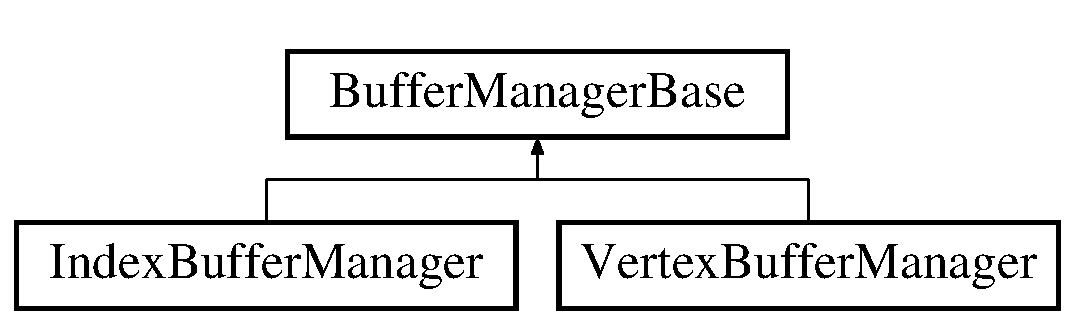
\includegraphics[height=2.000000cm]{d2/d01/class_buffer_manager_base}
\end{center}
\end{figure}
\subsection*{Public Member Functions}
\begin{DoxyCompactItemize}
\item 
\mbox{\hyperlink{stdafx_8h_a8ee2d990c5dfba7794dd2b60741d7722}{D3\+D\+E\+N\+G\+I\+N\+E\+\_\+\+A\+PI}} \mbox{\hyperlink{class_buffer_manager_base_a9cec2f80ae72dc972ef6d18ab075ab6c}{Buffer\+Manager\+Base}} (U\+I\+NT size, B\+Y\+TE $\ast$data, D3\+D12\+\_\+\+R\+E\+S\+O\+U\+R\+C\+E\+\_\+\+S\+T\+A\+T\+ES state, std\+::shared\+\_\+ptr$<$ \mbox{\hyperlink{class_d_x_1_1_device_resources}{D\+X\+::\+Device\+Resources}} $>$ device\+Resources, std\+::shared\+\_\+ptr$<$ \mbox{\hyperlink{class_command_list_manager}{Command\+List\+Manager}} $>$ command\+List\+Manager)
\begin{DoxyCompactList}\small\item\em Construct a new Buffer Manager Base\+:\+: Buffer Manager Base object. \end{DoxyCompactList}\item 
\mbox{\hyperlink{stdafx_8h_a8ee2d990c5dfba7794dd2b60741d7722}{D3\+D\+E\+N\+G\+I\+N\+E\+\_\+\+A\+PI}} \mbox{\hyperlink{class_buffer_manager_base_af579a9443cc34b2526a38b87b437c895}{$\sim$\+Buffer\+Manager\+Base}} ()
\item 
\mbox{\hyperlink{stdafx_8h_a8ee2d990c5dfba7794dd2b60741d7722}{D3\+D\+E\+N\+G\+I\+N\+E\+\_\+\+A\+PI}} I\+D3\+D12\+Resource $\ast$ \mbox{\hyperlink{class_buffer_manager_base_afa03f652ef76e70618f7f112b7da48c5}{Get\+Resource}} () const
\end{DoxyCompactItemize}
\subsection*{Private Attributes}
\begin{DoxyCompactItemize}
\item 
std\+::unique\+\_\+ptr$<$ \mbox{\hyperlink{class_resource_manager}{Resource\+Manager}} $>$ \mbox{\hyperlink{class_buffer_manager_base_a1477064838478bbbf233da29598a2352}{m\+\_\+resource\+Manager}}
\end{DoxyCompactItemize}


\subsection{Detailed Description}


Definition at line 7 of file Buffer\+Manager\+Base.\+h.



\subsection{Constructor \& Destructor Documentation}
\mbox{\Hypertarget{class_buffer_manager_base_a9cec2f80ae72dc972ef6d18ab075ab6c}\label{class_buffer_manager_base_a9cec2f80ae72dc972ef6d18ab075ab6c}} 
\index{Buffer\+Manager\+Base@{Buffer\+Manager\+Base}!Buffer\+Manager\+Base@{Buffer\+Manager\+Base}}
\index{Buffer\+Manager\+Base@{Buffer\+Manager\+Base}!Buffer\+Manager\+Base@{Buffer\+Manager\+Base}}
\subsubsection{\texorpdfstring{Buffer\+Manager\+Base()}{BufferManagerBase()}}
{\footnotesize\ttfamily Buffer\+Manager\+Base\+::\+Buffer\+Manager\+Base (\begin{DoxyParamCaption}\item[{U\+I\+NT}]{size,  }\item[{B\+Y\+TE $\ast$}]{data,  }\item[{D3\+D12\+\_\+\+R\+E\+S\+O\+U\+R\+C\+E\+\_\+\+S\+T\+A\+T\+ES}]{state,  }\item[{std\+::shared\+\_\+ptr$<$ \mbox{\hyperlink{class_d_x_1_1_device_resources}{D\+X\+::\+Device\+Resources}} $>$}]{device\+Resources,  }\item[{std\+::shared\+\_\+ptr$<$ \mbox{\hyperlink{class_command_list_manager}{Command\+List\+Manager}} $>$}]{command\+List\+Manager }\end{DoxyParamCaption})}



Construct a new Buffer Manager Base\+:\+: Buffer Manager Base object. 


\begin{DoxyParams}{Parameters}
{\em size} & size of the buffer \\
\hline
{\em data} & the data that will be sent to the G\+PU \\
\hline
{\em state} & the resource state \\
\hline
{\em device\+Resources} & \\
\hline
{\em command\+List\+Manager} & \\
\hline
\end{DoxyParams}


Definition at line 13 of file Buffer\+Manager\+Base.\+cpp.


\begin{DoxyCode}
15 \{
16     \textcolor{keyword}{const} CD3DX12\_RESOURCE\_DESC bufferDesc = CD3DX12\_RESOURCE\_DESC::Buffer(size);
17     \mbox{\hyperlink{class_buffer_manager_base_a1477064838478bbbf233da29598a2352}{m\_resourceManager}} = std::make\_unique<ResourceManager>(
18         \mbox{\hyperlink{class_resource_manager}{ResourceManager}}(deviceResources, commandListManager));
19     \mbox{\hyperlink{class_buffer_manager_base_a1477064838478bbbf233da29598a2352}{m\_resourceManager}}->DefaultHeapResource(bufferDesc);
20     \mbox{\hyperlink{class_buffer_manager_base_a1477064838478bbbf233da29598a2352}{m\_resourceManager}}->UploadResource(bufferDesc);
21     
22     \mbox{\hyperlink{class_buffer_manager_base_a1477064838478bbbf233da29598a2352}{m\_resourceManager}}->UpdateSubresource(data, size, size, size, state);
23 \}
\end{DoxyCode}
\mbox{\Hypertarget{class_buffer_manager_base_af579a9443cc34b2526a38b87b437c895}\label{class_buffer_manager_base_af579a9443cc34b2526a38b87b437c895}} 
\index{Buffer\+Manager\+Base@{Buffer\+Manager\+Base}!````~Buffer\+Manager\+Base@{$\sim$\+Buffer\+Manager\+Base}}
\index{````~Buffer\+Manager\+Base@{$\sim$\+Buffer\+Manager\+Base}!Buffer\+Manager\+Base@{Buffer\+Manager\+Base}}
\subsubsection{\texorpdfstring{$\sim$\+Buffer\+Manager\+Base()}{~BufferManagerBase()}}
{\footnotesize\ttfamily Buffer\+Manager\+Base\+::$\sim$\+Buffer\+Manager\+Base (\begin{DoxyParamCaption}{ }\end{DoxyParamCaption})}



Definition at line 25 of file Buffer\+Manager\+Base.\+cpp.


\begin{DoxyCode}
26 \{
27 
28     \mbox{\hyperlink{class_buffer_manager_base_a1477064838478bbbf233da29598a2352}{m\_resourceManager}}.release();
29     \mbox{\hyperlink{class_buffer_manager_base_a1477064838478bbbf233da29598a2352}{m\_resourceManager}} = \textcolor{keyword}{nullptr};
30 \}
\end{DoxyCode}


\subsection{Member Function Documentation}
\mbox{\Hypertarget{class_buffer_manager_base_afa03f652ef76e70618f7f112b7da48c5}\label{class_buffer_manager_base_afa03f652ef76e70618f7f112b7da48c5}} 
\index{Buffer\+Manager\+Base@{Buffer\+Manager\+Base}!Get\+Resource@{Get\+Resource}}
\index{Get\+Resource@{Get\+Resource}!Buffer\+Manager\+Base@{Buffer\+Manager\+Base}}
\subsubsection{\texorpdfstring{Get\+Resource()}{GetResource()}}
{\footnotesize\ttfamily \mbox{\hyperlink{stdafx_8h_a8ee2d990c5dfba7794dd2b60741d7722}{D3\+D\+E\+N\+G\+I\+N\+E\+\_\+\+A\+PI}} I\+D3\+D12\+Resource$\ast$ Buffer\+Manager\+Base\+::\+Get\+Resource (\begin{DoxyParamCaption}{ }\end{DoxyParamCaption}) const\hspace{0.3cm}{\ttfamily [inline]}}



Definition at line 14 of file Buffer\+Manager\+Base.\+h.


\begin{DoxyCode}
14 \{ \textcolor{keywordflow}{return} \mbox{\hyperlink{class_buffer_manager_base_a1477064838478bbbf233da29598a2352}{m\_resourceManager}}->Get(); \};
\end{DoxyCode}


\subsection{Member Data Documentation}
\mbox{\Hypertarget{class_buffer_manager_base_a1477064838478bbbf233da29598a2352}\label{class_buffer_manager_base_a1477064838478bbbf233da29598a2352}} 
\index{Buffer\+Manager\+Base@{Buffer\+Manager\+Base}!m\+\_\+resource\+Manager@{m\+\_\+resource\+Manager}}
\index{m\+\_\+resource\+Manager@{m\+\_\+resource\+Manager}!Buffer\+Manager\+Base@{Buffer\+Manager\+Base}}
\subsubsection{\texorpdfstring{m\+\_\+resource\+Manager}{m\_resourceManager}}
{\footnotesize\ttfamily std\+::unique\+\_\+ptr$<$\mbox{\hyperlink{class_resource_manager}{Resource\+Manager}}$>$ Buffer\+Manager\+Base\+::m\+\_\+resource\+Manager\hspace{0.3cm}{\ttfamily [private]}}



Definition at line 14 of file Buffer\+Manager\+Base.\+h.



The documentation for this class was generated from the following files\+:\begin{DoxyCompactItemize}
\item 
D3d\+Engine/\mbox{\hyperlink{_buffer_manager_base_8h}{Buffer\+Manager\+Base.\+h}}\item 
D3d\+Engine/\mbox{\hyperlink{_buffer_manager_base_8cpp}{Buffer\+Manager\+Base.\+cpp}}\end{DoxyCompactItemize}

\hypertarget{class_camera_helper}{}\section{Camera\+Helper Class Reference}
\label{class_camera_helper}\index{Camera\+Helper@{Camera\+Helper}}


{\ttfamily \#include $<$Camera\+Helper.\+h$>$}

\subsection*{Public Member Functions}
\begin{DoxyCompactItemize}
\item 
\mbox{\hyperlink{stdafx_8h_a8ee2d990c5dfba7794dd2b60741d7722}{D3\+D\+E\+N\+G\+I\+N\+E\+\_\+\+A\+PI}} \mbox{\hyperlink{class_camera_helper_a401e32c823d85e9dedeebfd67318e557}{Camera\+Helper}} (std\+::shared\+\_\+ptr$<$ \mbox{\hyperlink{class_d_x_1_1_device_resources}{D\+X\+::\+Device\+Resources}} $>$ device\+Resources)
\item 
\mbox{\hyperlink{stdafx_8h_a8ee2d990c5dfba7794dd2b60741d7722}{D3\+D\+E\+N\+G\+I\+N\+E\+\_\+\+A\+PI}} \mbox{\hyperlink{class_camera_helper_af339b23a92498ca44946c589a7004837}{$\sim$\+Camera\+Helper}} ()
\item 
\mbox{\hyperlink{stdafx_8h_a8ee2d990c5dfba7794dd2b60741d7722}{D3\+D\+E\+N\+G\+I\+N\+E\+\_\+\+A\+PI}} void \mbox{\hyperlink{class_camera_helper_ac9033557a8988c86d0daf3aab1bbfa7f}{On\+Key\+Down}} (U\+I\+NT key)
\item 
\mbox{\hyperlink{stdafx_8h_a8ee2d990c5dfba7794dd2b60741d7722}{D3\+D\+E\+N\+G\+I\+N\+E\+\_\+\+A\+PI}} void \mbox{\hyperlink{class_camera_helper_ab7a651ac749461d078779b8c0accd9a7}{On\+Key\+Up}} (U\+I\+NT key)
\item 
\mbox{\hyperlink{stdafx_8h_a8ee2d990c5dfba7794dd2b60741d7722}{D3\+D\+E\+N\+G\+I\+N\+E\+\_\+\+A\+PI}} void \mbox{\hyperlink{class_camera_helper_a0b9c762c778086dd01d90a25b7ea2989}{Update}} (X\+M\+V\+E\+C\+T\+OR $\ast$pos)
\item 
\mbox{\hyperlink{stdafx_8h_a8ee2d990c5dfba7794dd2b60741d7722}{D3\+D\+E\+N\+G\+I\+N\+E\+\_\+\+A\+PI}} void \mbox{\hyperlink{class_camera_helper_add97d2d08199687ac37111773001bb10}{On\+Mouse\+Moved}} (float x, float y)
\item 
\mbox{\hyperlink{stdafx_8h_a8ee2d990c5dfba7794dd2b60741d7722}{D3\+D\+E\+N\+G\+I\+N\+E\+\_\+\+A\+PI}} bool \mbox{\hyperlink{class_camera_helper_a1801645e4919706fe53c2d8bc2683933}{Get\+Is\+Jumping}} () const
\item 
\mbox{\hyperlink{stdafx_8h_a8ee2d990c5dfba7794dd2b60741d7722}{D3\+D\+E\+N\+G\+I\+N\+E\+\_\+\+A\+PI}} void \mbox{\hyperlink{class_camera_helper_a2fc6faa8ce769fdedee3802719c2f372}{On\+Window\+Size\+Changed}} ()
\begin{DoxyCompactList}\small\item\em Called when the window size is changed s Sets the perspective matrix from the \mbox{\hyperlink{class_model_view_projection_manager}{Model\+View\+Projection\+Manager}} and the m\+\_\+scissor\+Rect. \end{DoxyCompactList}\item 
\mbox{\hyperlink{stdafx_8h_a8ee2d990c5dfba7794dd2b60741d7722}{D3\+D\+E\+N\+G\+I\+N\+E\+\_\+\+A\+PI}} D3\+D12\+\_\+\+R\+E\+CT \mbox{\hyperlink{class_camera_helper_a75e575bef9dd1e3f6b2608be1b5f15b7}{Get\+Scissor\+Rect}} () const
\item 
\mbox{\hyperlink{stdafx_8h_a8ee2d990c5dfba7794dd2b60741d7722}{D3\+D\+E\+N\+G\+I\+N\+E\+\_\+\+A\+PI}} X\+M\+V\+E\+C\+T\+OR \mbox{\hyperlink{class_camera_helper_a142721c2285930e8fa5f5674c6196688}{Get\+Position}} () const
\item 
\mbox{\hyperlink{stdafx_8h_a8ee2d990c5dfba7794dd2b60741d7722}{D3\+D\+E\+N\+G\+I\+N\+E\+\_\+\+A\+PI}} X\+M\+V\+E\+C\+T\+OR \mbox{\hyperlink{class_camera_helper_a26e57d260f821f47b9fd5ca456d25e7c}{Get\+Camera\+Position}} () const
\item 
\mbox{\hyperlink{stdafx_8h_a8ee2d990c5dfba7794dd2b60741d7722}{D3\+D\+E\+N\+G\+I\+N\+E\+\_\+\+A\+PI}} float \mbox{\hyperlink{class_camera_helper_a82e6dc2802d286a719c07b3d8484f139}{Get\+Camera\+Rot\+Yaw}} () const
\item 
\mbox{\hyperlink{stdafx_8h_a8ee2d990c5dfba7794dd2b60741d7722}{D3\+D\+E\+N\+G\+I\+N\+E\+\_\+\+A\+PI}} \mbox{\hyperlink{struct_structures_1_1_model_view_projection_constant_buffer}{Structures\+::\+Model\+View\+Projection\+Constant\+Buffer}} \mbox{\hyperlink{class_camera_helper_a52e1cde25a6b6486dc9df5f25ae695d2}{Get\+Cbv\+Data}} ()
\end{DoxyCompactItemize}
\subsection*{Private Attributes}
\begin{DoxyCompactItemize}
\item 
std\+::shared\+\_\+ptr$<$ \mbox{\hyperlink{class_d_x_1_1_device_resources}{D\+X\+::\+Device\+Resources}} $>$ \mbox{\hyperlink{class_camera_helper_a68562f65262d3c90532df0a194624ec9}{m\+\_\+device\+Resources}}
\item 
std\+::shared\+\_\+ptr$<$ \mbox{\hyperlink{class_model_view_projection_manager}{Model\+View\+Projection\+Manager}} $>$ \mbox{\hyperlink{class_camera_helper_a10d96783299a8c958f84d46542a3d93f}{m\+\_\+mvp\+Manager}}
\begin{DoxyCompactList}\small\item\em The D3d Device manager class. \end{DoxyCompactList}\item 
std\+::unique\+\_\+ptr$<$ \mbox{\hyperlink{class_terrain_collision_helper}{Terrain\+Collision\+Helper}} $>$ \mbox{\hyperlink{class_camera_helper_a5ce949723d775603a605ffcd9cc68bbc}{m\+\_\+terrain\+Collider}}
\begin{DoxyCompactList}\small\item\em The Model View Perspective matrices manager. \end{DoxyCompactList}\item 
float \mbox{\hyperlink{class_camera_helper_ae2a32d581a829b05300d7298b5622469}{m\+\_\+pitch}}
\begin{DoxyCompactList}\small\item\em Terrain Collision detecter and manager. \end{DoxyCompactList}\item 
float \mbox{\hyperlink{class_camera_helper_a9bdda4839839b4329188fc44517e8b01}{m\+\_\+yaw}}
\begin{DoxyCompactList}\small\item\em The pitch of the mouse movement. \end{DoxyCompactList}\item 
Direct\+X\+::\+X\+M\+V\+E\+C\+T\+O\+R\+F32 \mbox{\hyperlink{class_camera_helper_af2822e6b05e48f33100c2f678e3776ce}{m\+\_\+direction}}
\begin{DoxyCompactList}\small\item\em The yaw of the mouse movement. \end{DoxyCompactList}\item 
Direct\+X\+::\+X\+M\+V\+E\+C\+T\+O\+R\+F32 \mbox{\hyperlink{class_camera_helper_a9f225b52b05df432872e8b541079935f}{m\+\_\+position}}
\begin{DoxyCompactList}\small\item\em The direction the keys have been pressed to form. \end{DoxyCompactList}\item 
Direct\+X\+::\+X\+M\+M\+A\+T\+R\+IX \mbox{\hyperlink{class_camera_helper_a995de11be349b7d74075f08fa5e2f437}{m\+\_\+cam\+Rotation\+Matrix}}
\begin{DoxyCompactList}\small\item\em The position of the camera. \end{DoxyCompactList}\item 
Direct\+X\+::\+X\+M\+V\+E\+C\+T\+OR \mbox{\hyperlink{class_camera_helper_a4f5d97db4f91d138f5ea4bf4416df132}{Default\+Forward}} = Direct\+X\+::\+X\+M\+Vector\+Set(0.\+0f, 0.\+0f, 1.\+0f, 0.\+0f)
\begin{DoxyCompactList}\small\item\em The rotation matrix of the camera. \end{DoxyCompactList}\item 
Direct\+X\+::\+X\+M\+V\+E\+C\+T\+OR \mbox{\hyperlink{class_camera_helper_af4ca47176953088f0f18adecf7bf4409}{Default\+Right}} = Direct\+X\+::\+X\+M\+Vector\+Set(1.\+0f, 0.\+0f, 0.\+0f, 0.\+0f)
\begin{DoxyCompactList}\small\item\em The Default forward facing vector. \end{DoxyCompactList}\item 
Direct\+X\+::\+X\+M\+V\+E\+C\+T\+OR \mbox{\hyperlink{class_camera_helper_abc1a814a0b54bfcb70f3e24bcd444f01}{m\+\_\+cam\+Target}}
\begin{DoxyCompactList}\small\item\em The Default Right facing vector. \end{DoxyCompactList}\item 
D3\+D12\+\_\+\+R\+E\+CT \mbox{\hyperlink{class_camera_helper_add052fea87500f1d3b2732ec46c3ae85}{m\+\_\+scissor\+Rect}}
\begin{DoxyCompactList}\small\item\em The target that the camera will look at. \end{DoxyCompactList}\item 
bool \mbox{\hyperlink{class_camera_helper_ac0dd816f2a5e8b4030b62e703ab92861}{is\+Jumping}}
\begin{DoxyCompactList}\small\item\em Rect that anything outside of it will not be displayed. \end{DoxyCompactList}\item 
const float \mbox{\hyperlink{class_camera_helper_ac0b6f1a7975e28a7604985da3f29278b}{c\+\_\+camera\+Ground\+Offset}} = 2
\begin{DoxyCompactList}\small\item\em Is camera or player jumping. \end{DoxyCompactList}\item 
bool \mbox{\hyperlink{class_camera_helper_a58fe7fb37f0bda549c7a8cc59fb58042}{m\+\_\+is\+Under\+Ground}}
\begin{DoxyCompactList}\small\item\em The constant offset of the camera from the ground. \end{DoxyCompactList}\end{DoxyCompactItemize}


\subsection{Detailed Description}


Definition at line 7 of file Camera\+Helper.\+h.



\subsection{Constructor \& Destructor Documentation}
\mbox{\Hypertarget{class_camera_helper_a401e32c823d85e9dedeebfd67318e557}\label{class_camera_helper_a401e32c823d85e9dedeebfd67318e557}} 
\index{Camera\+Helper@{Camera\+Helper}!Camera\+Helper@{Camera\+Helper}}
\index{Camera\+Helper@{Camera\+Helper}!Camera\+Helper@{Camera\+Helper}}
\subsubsection{\texorpdfstring{Camera\+Helper()}{CameraHelper()}}
{\footnotesize\ttfamily Camera\+Helper\+::\+Camera\+Helper (\begin{DoxyParamCaption}\item[{std\+::shared\+\_\+ptr$<$ \mbox{\hyperlink{class_d_x_1_1_device_resources}{D\+X\+::\+Device\+Resources}} $>$}]{device\+Resources }\end{DoxyParamCaption})}

The Constructor Creates and initialises members of the class 
\begin{DoxyParams}{Parameters}
{\em device\+Resources} & the Direct3D Device manager \\
\hline
\end{DoxyParams}


Definition at line 12 of file Camera\+Helper.\+cpp.


\begin{DoxyCode}
13     : \mbox{\hyperlink{class_camera_helper_a68562f65262d3c90532df0a194624ec9}{m\_deviceResources}}(deviceResources),
14     \mbox{\hyperlink{class_camera_helper_ae2a32d581a829b05300d7298b5622469}{m\_pitch}}(0),
15     \mbox{\hyperlink{class_camera_helper_a9bdda4839839b4329188fc44517e8b01}{m\_yaw}}(0),
16     \mbox{\hyperlink{class_camera_helper_abc1a814a0b54bfcb70f3e24bcd444f01}{m\_camTarget}}(\{\}),
17     \mbox{\hyperlink{class_camera_helper_a9f225b52b05df432872e8b541079935f}{m\_position}}(\{ 0,0,0,0 \}),
18     \mbox{\hyperlink{class_camera_helper_af2822e6b05e48f33100c2f678e3776ce}{m\_direction}}(\{\}),
19     \mbox{\hyperlink{class_camera_helper_ac0dd816f2a5e8b4030b62e703ab92861}{isJumping}}(\textcolor{keyword}{false}),
20     \mbox{\hyperlink{class_camera_helper_a58fe7fb37f0bda549c7a8cc59fb58042}{m\_isUnderGround}}(\textcolor{keyword}{false})
21 \{
22     \textcolor{comment}{// Creates shared\_ptr of \(\backslash\)class TerrainCollisionHelper}
23     \mbox{\hyperlink{class_camera_helper_a5ce949723d775603a605ffcd9cc68bbc}{m\_terrainCollider}} = std::make\_unique<TerrainCollisionHelper>();
24     \textcolor{comment}{// Creates shared\_ptr of \(\backslash\)class ModelViewProjectionManager}
25     \mbox{\hyperlink{class_camera_helper_a10d96783299a8c958f84d46542a3d93f}{m\_mvpManager}} = std::make\_shared<ModelViewProjectionManager>();
26 \}
\end{DoxyCode}
\mbox{\Hypertarget{class_camera_helper_af339b23a92498ca44946c589a7004837}\label{class_camera_helper_af339b23a92498ca44946c589a7004837}} 
\index{Camera\+Helper@{Camera\+Helper}!````~Camera\+Helper@{$\sim$\+Camera\+Helper}}
\index{````~Camera\+Helper@{$\sim$\+Camera\+Helper}!Camera\+Helper@{Camera\+Helper}}
\subsubsection{\texorpdfstring{$\sim$\+Camera\+Helper()}{~CameraHelper()}}
{\footnotesize\ttfamily Camera\+Helper\+::$\sim$\+Camera\+Helper (\begin{DoxyParamCaption}{ }\end{DoxyParamCaption})}

The Deconstructor 

Definition at line 31 of file Camera\+Helper.\+cpp.


\begin{DoxyCode}
32 \{
33 \}
\end{DoxyCode}


\subsection{Member Function Documentation}
\mbox{\Hypertarget{class_camera_helper_a26e57d260f821f47b9fd5ca456d25e7c}\label{class_camera_helper_a26e57d260f821f47b9fd5ca456d25e7c}} 
\index{Camera\+Helper@{Camera\+Helper}!Get\+Camera\+Position@{Get\+Camera\+Position}}
\index{Get\+Camera\+Position@{Get\+Camera\+Position}!Camera\+Helper@{Camera\+Helper}}
\subsubsection{\texorpdfstring{Get\+Camera\+Position()}{GetCameraPosition()}}
{\footnotesize\ttfamily \mbox{\hyperlink{stdafx_8h_a8ee2d990c5dfba7794dd2b60741d7722}{D3\+D\+E\+N\+G\+I\+N\+E\+\_\+\+A\+PI}} X\+M\+V\+E\+C\+T\+OR Camera\+Helper\+::\+Get\+Camera\+Position (\begin{DoxyParamCaption}{ }\end{DoxyParamCaption}) const\hspace{0.3cm}{\ttfamily [inline]}}



Definition at line 28 of file Camera\+Helper.\+h.


\begin{DoxyCode}
28 \{ \textcolor{keywordflow}{return} \mbox{\hyperlink{class_camera_helper_abc1a814a0b54bfcb70f3e24bcd444f01}{m\_camTarget}}; \};
\end{DoxyCode}
\mbox{\Hypertarget{class_camera_helper_a82e6dc2802d286a719c07b3d8484f139}\label{class_camera_helper_a82e6dc2802d286a719c07b3d8484f139}} 
\index{Camera\+Helper@{Camera\+Helper}!Get\+Camera\+Rot\+Yaw@{Get\+Camera\+Rot\+Yaw}}
\index{Get\+Camera\+Rot\+Yaw@{Get\+Camera\+Rot\+Yaw}!Camera\+Helper@{Camera\+Helper}}
\subsubsection{\texorpdfstring{Get\+Camera\+Rot\+Yaw()}{GetCameraRotYaw()}}
{\footnotesize\ttfamily \mbox{\hyperlink{stdafx_8h_a8ee2d990c5dfba7794dd2b60741d7722}{D3\+D\+E\+N\+G\+I\+N\+E\+\_\+\+A\+PI}} float Camera\+Helper\+::\+Get\+Camera\+Rot\+Yaw (\begin{DoxyParamCaption}{ }\end{DoxyParamCaption}) const\hspace{0.3cm}{\ttfamily [inline]}}



Definition at line 29 of file Camera\+Helper.\+h.


\begin{DoxyCode}
29 \{ \textcolor{keywordflow}{return} \mbox{\hyperlink{class_camera_helper_a9bdda4839839b4329188fc44517e8b01}{m\_yaw}}; \};
\end{DoxyCode}
\mbox{\Hypertarget{class_camera_helper_a52e1cde25a6b6486dc9df5f25ae695d2}\label{class_camera_helper_a52e1cde25a6b6486dc9df5f25ae695d2}} 
\index{Camera\+Helper@{Camera\+Helper}!Get\+Cbv\+Data@{Get\+Cbv\+Data}}
\index{Get\+Cbv\+Data@{Get\+Cbv\+Data}!Camera\+Helper@{Camera\+Helper}}
\subsubsection{\texorpdfstring{Get\+Cbv\+Data()}{GetCbvData()}}
{\footnotesize\ttfamily \mbox{\hyperlink{struct_structures_1_1_model_view_projection_constant_buffer}{Structures\+::\+Model\+View\+Projection\+Constant\+Buffer}} Camera\+Helper\+::\+Get\+Cbv\+Data (\begin{DoxyParamCaption}{ }\end{DoxyParamCaption})}



Definition at line 262 of file Camera\+Helper.\+cpp.


\begin{DoxyCode}
263 \{
264     \textcolor{keywordflow}{return} \mbox{\hyperlink{class_camera_helper_a10d96783299a8c958f84d46542a3d93f}{m\_mvpManager}}->GetCbvData();
265 \}
\end{DoxyCode}
\mbox{\Hypertarget{class_camera_helper_a1801645e4919706fe53c2d8bc2683933}\label{class_camera_helper_a1801645e4919706fe53c2d8bc2683933}} 
\index{Camera\+Helper@{Camera\+Helper}!Get\+Is\+Jumping@{Get\+Is\+Jumping}}
\index{Get\+Is\+Jumping@{Get\+Is\+Jumping}!Camera\+Helper@{Camera\+Helper}}
\subsubsection{\texorpdfstring{Get\+Is\+Jumping()}{GetIsJumping()}}
{\footnotesize\ttfamily \mbox{\hyperlink{stdafx_8h_a8ee2d990c5dfba7794dd2b60741d7722}{D3\+D\+E\+N\+G\+I\+N\+E\+\_\+\+A\+PI}} bool Camera\+Helper\+::\+Get\+Is\+Jumping (\begin{DoxyParamCaption}{ }\end{DoxyParamCaption}) const\hspace{0.3cm}{\ttfamily [inline]}}



Definition at line 23 of file Camera\+Helper.\+h.


\begin{DoxyCode}
23 \{ \textcolor{keywordflow}{return} \mbox{\hyperlink{class_camera_helper_ac0dd816f2a5e8b4030b62e703ab92861}{isJumping}}; \};
\end{DoxyCode}
\mbox{\Hypertarget{class_camera_helper_a142721c2285930e8fa5f5674c6196688}\label{class_camera_helper_a142721c2285930e8fa5f5674c6196688}} 
\index{Camera\+Helper@{Camera\+Helper}!Get\+Position@{Get\+Position}}
\index{Get\+Position@{Get\+Position}!Camera\+Helper@{Camera\+Helper}}
\subsubsection{\texorpdfstring{Get\+Position()}{GetPosition()}}
{\footnotesize\ttfamily \mbox{\hyperlink{stdafx_8h_a8ee2d990c5dfba7794dd2b60741d7722}{D3\+D\+E\+N\+G\+I\+N\+E\+\_\+\+A\+PI}} X\+M\+V\+E\+C\+T\+OR Camera\+Helper\+::\+Get\+Position (\begin{DoxyParamCaption}{ }\end{DoxyParamCaption}) const\hspace{0.3cm}{\ttfamily [inline]}}



Definition at line 27 of file Camera\+Helper.\+h.


\begin{DoxyCode}
27 \{ \textcolor{keywordflow}{return} \mbox{\hyperlink{class_camera_helper_a9f225b52b05df432872e8b541079935f}{m\_position}}; \};
\end{DoxyCode}
\mbox{\Hypertarget{class_camera_helper_a75e575bef9dd1e3f6b2608be1b5f15b7}\label{class_camera_helper_a75e575bef9dd1e3f6b2608be1b5f15b7}} 
\index{Camera\+Helper@{Camera\+Helper}!Get\+Scissor\+Rect@{Get\+Scissor\+Rect}}
\index{Get\+Scissor\+Rect@{Get\+Scissor\+Rect}!Camera\+Helper@{Camera\+Helper}}
\subsubsection{\texorpdfstring{Get\+Scissor\+Rect()}{GetScissorRect()}}
{\footnotesize\ttfamily \mbox{\hyperlink{stdafx_8h_a8ee2d990c5dfba7794dd2b60741d7722}{D3\+D\+E\+N\+G\+I\+N\+E\+\_\+\+A\+PI}} D3\+D12\+\_\+\+R\+E\+CT Camera\+Helper\+::\+Get\+Scissor\+Rect (\begin{DoxyParamCaption}{ }\end{DoxyParamCaption}) const\hspace{0.3cm}{\ttfamily [inline]}}



Definition at line 26 of file Camera\+Helper.\+h.


\begin{DoxyCode}
26 \{ \textcolor{keywordflow}{return} \mbox{\hyperlink{class_camera_helper_add052fea87500f1d3b2732ec46c3ae85}{m\_scissorRect}}; \};
\end{DoxyCode}
\mbox{\Hypertarget{class_camera_helper_ac9033557a8988c86d0daf3aab1bbfa7f}\label{class_camera_helper_ac9033557a8988c86d0daf3aab1bbfa7f}} 
\index{Camera\+Helper@{Camera\+Helper}!On\+Key\+Down@{On\+Key\+Down}}
\index{On\+Key\+Down@{On\+Key\+Down}!Camera\+Helper@{Camera\+Helper}}
\subsubsection{\texorpdfstring{On\+Key\+Down()}{OnKeyDown()}}
{\footnotesize\ttfamily void Camera\+Helper\+::\+On\+Key\+Down (\begin{DoxyParamCaption}\item[{U\+I\+NT}]{key }\end{DoxyParamCaption})}

Gets key presses to move the camera and player Changes the direction of movement doesn\textquotesingle{}t move anything 
\begin{DoxyParams}{Parameters}
{\em key} & the unsigned integer key code for the key that has been pressed \\
\hline
\end{DoxyParams}


Definition at line 40 of file Camera\+Helper.\+cpp.


\begin{DoxyCode}
41 \{
42     \textcolor{comment}{// Set \(\backslash\)property m\_direction to forward on "W" pressed}
43     \textcolor{keywordflow}{if} (key == 0x57)
44     \{
45         \mbox{\hyperlink{class_camera_helper_af2822e6b05e48f33100c2f678e3776ce}{m\_direction}}.v = XMVectorSetZ(\mbox{\hyperlink{class_camera_helper_af2822e6b05e48f33100c2f678e3776ce}{m\_direction}}, 1);
46     \}
47     \textcolor{comment}{// Set \(\backslash\)property m\_direction to left on "A" pressed}
48     \textcolor{keywordflow}{else} \textcolor{keywordflow}{if} (key == 0x41)
49     \{
50         \mbox{\hyperlink{class_camera_helper_af2822e6b05e48f33100c2f678e3776ce}{m\_direction}}.v = XMVectorSetX(\mbox{\hyperlink{class_camera_helper_af2822e6b05e48f33100c2f678e3776ce}{m\_direction}}, 1);
51     \}
52     \textcolor{comment}{// Set \(\backslash\)property m\_direction to backward on "S" pressed}
53     \textcolor{keywordflow}{else} \textcolor{keywordflow}{if} (key == 0x53)
54     \{
55         \mbox{\hyperlink{class_camera_helper_af2822e6b05e48f33100c2f678e3776ce}{m\_direction}}.v = XMVectorSetZ(\mbox{\hyperlink{class_camera_helper_af2822e6b05e48f33100c2f678e3776ce}{m\_direction}}, -1);
56     \}
57     \textcolor{comment}{// Set \(\backslash\)property m\_direction to right on "D" pressed}
58     \textcolor{keywordflow}{else} \textcolor{keywordflow}{if} (key == 0x44)
59     \{
60         \mbox{\hyperlink{class_camera_helper_af2822e6b05e48f33100c2f678e3776ce}{m\_direction}}.v = XMVectorSetX(\mbox{\hyperlink{class_camera_helper_af2822e6b05e48f33100c2f678e3776ce}{m\_direction}}, -1);
61     \}
62     \textcolor{comment}{// Set \(\backslash\)property m\_direction to up on "SpaceBar" pressed}
63     \textcolor{keywordflow}{else} \textcolor{keywordflow}{if} (key == VK\_SPACE)
64     \{
65         \mbox{\hyperlink{class_camera_helper_ac0dd816f2a5e8b4030b62e703ab92861}{isJumping}} = \textcolor{keyword}{true};
66         \mbox{\hyperlink{class_camera_helper_af2822e6b05e48f33100c2f678e3776ce}{m\_direction}}.v = XMVectorSetY(\mbox{\hyperlink{class_camera_helper_af2822e6b05e48f33100c2f678e3776ce}{m\_direction}}, 1);
67     \}
68     \textcolor{comment}{// Set \(\backslash\)property m\_direction to down on "Shift" pressed}
69     \textcolor{keywordflow}{else} \textcolor{keywordflow}{if} (key == VK\_SHIFT)
70     \{
71         \mbox{\hyperlink{class_camera_helper_af2822e6b05e48f33100c2f678e3776ce}{m\_direction}}.v = XMVectorSetY(\mbox{\hyperlink{class_camera_helper_af2822e6b05e48f33100c2f678e3776ce}{m\_direction}}, -1);
72     \}
73 \}
\end{DoxyCode}
\mbox{\Hypertarget{class_camera_helper_ab7a651ac749461d078779b8c0accd9a7}\label{class_camera_helper_ab7a651ac749461d078779b8c0accd9a7}} 
\index{Camera\+Helper@{Camera\+Helper}!On\+Key\+Up@{On\+Key\+Up}}
\index{On\+Key\+Up@{On\+Key\+Up}!Camera\+Helper@{Camera\+Helper}}
\subsubsection{\texorpdfstring{On\+Key\+Up()}{OnKeyUp()}}
{\footnotesize\ttfamily void Camera\+Helper\+::\+On\+Key\+Up (\begin{DoxyParamCaption}\item[{U\+I\+NT}]{key }\end{DoxyParamCaption})}

Gets key presses to stop moving the camera and player Changes the direction of movement doesn\textquotesingle{}t move anything 
\begin{DoxyParams}{Parameters}
{\em key} & the unsigned integer key code for the key that has been released \\
\hline
\end{DoxyParams}


Definition at line 80 of file Camera\+Helper.\+cpp.


\begin{DoxyCode}
81 \{
82     \textcolor{comment}{// Set \(\backslash\)property m\_direction to forward on "W" pressed}
83     \textcolor{keywordflow}{if} (key == 0x57)
84     \{
85         \mbox{\hyperlink{class_camera_helper_af2822e6b05e48f33100c2f678e3776ce}{m\_direction}}.v = XMVectorSetZ(\mbox{\hyperlink{class_camera_helper_af2822e6b05e48f33100c2f678e3776ce}{m\_direction}}, 0);
86     \}
87     \textcolor{comment}{// Set \(\backslash\)property m\_direction to not left on "A" pressed}
88     \textcolor{keywordflow}{else} \textcolor{keywordflow}{if} (key == 0x41)
89     \{
90         \mbox{\hyperlink{class_camera_helper_af2822e6b05e48f33100c2f678e3776ce}{m\_direction}}.v = XMVectorSetX(\mbox{\hyperlink{class_camera_helper_af2822e6b05e48f33100c2f678e3776ce}{m\_direction}}, 0);
91     \}
92     \textcolor{comment}{// Set \(\backslash\)property m\_direction to not backward on "S" pressed}
93     \textcolor{keywordflow}{else} \textcolor{keywordflow}{if} (key == 0x53)
94     \{
95         \mbox{\hyperlink{class_camera_helper_af2822e6b05e48f33100c2f678e3776ce}{m\_direction}}.v = XMVectorSetZ(\mbox{\hyperlink{class_camera_helper_af2822e6b05e48f33100c2f678e3776ce}{m\_direction}}, 0);
96     \}
97     \textcolor{comment}{// Set \(\backslash\)property m\_direction to not right on "D" pressed}
98     \textcolor{keywordflow}{else} \textcolor{keywordflow}{if} (key == 0x44)
99     \{
100         \mbox{\hyperlink{class_camera_helper_af2822e6b05e48f33100c2f678e3776ce}{m\_direction}}.v = XMVectorSetX(\mbox{\hyperlink{class_camera_helper_af2822e6b05e48f33100c2f678e3776ce}{m\_direction}}, 0);
101     \}
102     \textcolor{comment}{// Set \(\backslash\)property m\_direction to not up on "SpaceBar" pressed}
103     \textcolor{keywordflow}{else} \textcolor{keywordflow}{if} (key == VK\_SPACE)
104     \{
105         \mbox{\hyperlink{class_camera_helper_ac0dd816f2a5e8b4030b62e703ab92861}{isJumping}} = \textcolor{keyword}{false};
106         \mbox{\hyperlink{class_camera_helper_af2822e6b05e48f33100c2f678e3776ce}{m\_direction}}.v = XMVectorSetY(\mbox{\hyperlink{class_camera_helper_af2822e6b05e48f33100c2f678e3776ce}{m\_direction}}, 0);
107     \}
108     \textcolor{comment}{// Set \(\backslash\)property m\_direction to not down on "Shift" pressed}
109     \textcolor{keywordflow}{else} \textcolor{keywordflow}{if} (key == VK\_SHIFT)
110     \{
111         \mbox{\hyperlink{class_camera_helper_af2822e6b05e48f33100c2f678e3776ce}{m\_direction}}.v = XMVectorSetY(\mbox{\hyperlink{class_camera_helper_af2822e6b05e48f33100c2f678e3776ce}{m\_direction}}, 0);
112     \}
113 \}
\end{DoxyCode}
\mbox{\Hypertarget{class_camera_helper_add97d2d08199687ac37111773001bb10}\label{class_camera_helper_add97d2d08199687ac37111773001bb10}} 
\index{Camera\+Helper@{Camera\+Helper}!On\+Mouse\+Moved@{On\+Mouse\+Moved}}
\index{On\+Mouse\+Moved@{On\+Mouse\+Moved}!Camera\+Helper@{Camera\+Helper}}
\subsubsection{\texorpdfstring{On\+Mouse\+Moved()}{OnMouseMoved()}}
{\footnotesize\ttfamily void Camera\+Helper\+::\+On\+Mouse\+Moved (\begin{DoxyParamCaption}\item[{float}]{x,  }\item[{float}]{y }\end{DoxyParamCaption})}

When the mouse is moved the function is called and the m\+\_\+pitch and m\+\_\+yaw are set to values which are relative to the new mouse movement the mouse movement is subtracted from the current m\+\_\+pitch and m\+\_\+yaw to achive smooth movement and cummulative movement (adds up) 
\begin{DoxyParams}{Parameters}
{\em x} & the horizonal movement of the mouse \\
\hline
{\em y} & the vertical movement of the mouse \\
\hline
\end{DoxyParams}


Definition at line 198 of file Camera\+Helper.\+cpp.


\begin{DoxyCode}
199 \{
200     \textcolor{comment}{// Multiplyer of the relative \(\backslash\)param x  \(\backslash\)param y;}
201     \textcolor{keyword}{const} \textcolor{keyword}{auto} multiplyer = 0.003f;
202     \textcolor{comment}{// is touching or under the terrain (see \(\backslash\)fn void CameraHelper::Update(XMVECTOR* pos) )}
203     \textcolor{keywordflow}{if} ((y < 0 && \mbox{\hyperlink{class_camera_helper_a58fe7fb37f0bda549c7a8cc59fb58042}{m\_isUnderGround}}) || !\mbox{\hyperlink{class_camera_helper_a58fe7fb37f0bda549c7a8cc59fb58042}{m\_isUnderGround}}) \{
204         \textcolor{comment}{// subtracts \(\backslash\)param y multiplied by \(\backslash\)var multiplyer to get the new \(\backslash\)property m\_pitch}
205         \mbox{\hyperlink{class_camera_helper_ae2a32d581a829b05300d7298b5622469}{m\_pitch}} -= y * multiplyer;
206     \}
207 
208     \textcolor{comment}{// subtracts negative \(\backslash\)param x multiplied by \(\backslash\)var multiplyer to get the new \(\backslash\)property m\_yaw}
209     \mbox{\hyperlink{class_camera_helper_a9bdda4839839b4329188fc44517e8b01}{m\_yaw}} -= -x * multiplyer;
210 
211     \textcolor{comment}{// Stops the rotations from going past half a circle}
212     \mbox{\hyperlink{class_camera_helper_ae2a32d581a829b05300d7298b5622469}{m\_pitch}} = (float)\_\_max(-DirectX::XM\_PI / 2.0f - 0.00003f, \mbox{\hyperlink{class_camera_helper_ae2a32d581a829b05300d7298b5622469}{m\_pitch}});
213     \mbox{\hyperlink{class_camera_helper_ae2a32d581a829b05300d7298b5622469}{m\_pitch}} = (float)\_\_min(+DirectX::XM\_PI / 2.0f - 0.00003f, \mbox{\hyperlink{class_camera_helper_ae2a32d581a829b05300d7298b5622469}{m\_pitch}});
214 \}
\end{DoxyCode}
\mbox{\Hypertarget{class_camera_helper_a2fc6faa8ce769fdedee3802719c2f372}\label{class_camera_helper_a2fc6faa8ce769fdedee3802719c2f372}} 
\index{Camera\+Helper@{Camera\+Helper}!On\+Window\+Size\+Changed@{On\+Window\+Size\+Changed}}
\index{On\+Window\+Size\+Changed@{On\+Window\+Size\+Changed}!Camera\+Helper@{Camera\+Helper}}
\subsubsection{\texorpdfstring{On\+Window\+Size\+Changed()}{OnWindowSizeChanged()}}
{\footnotesize\ttfamily void Camera\+Helper\+::\+On\+Window\+Size\+Changed (\begin{DoxyParamCaption}{ }\end{DoxyParamCaption})}



Called when the window size is changed s Sets the perspective matrix from the \mbox{\hyperlink{class_model_view_projection_manager}{Model\+View\+Projection\+Manager}} and the m\+\_\+scissor\+Rect. 



Definition at line 220 of file Camera\+Helper.\+cpp.


\begin{DoxyCode}
221 \{
222     \textcolor{comment}{// Gets thye inner window (output size) form \(\backslash\)class DeviceResources}
223     \textcolor{keyword}{const} \textcolor{keyword}{auto} outputSize = \mbox{\hyperlink{class_camera_helper_a68562f65262d3c90532df0a194624ec9}{m\_deviceResources}}->GetOutputSize();
224     \textcolor{comment}{// Gets aspect ratio from output size}
225     \textcolor{keyword}{const} \textcolor{keywordtype}{float} aspectRatio = outputSize.x / outputSize.y;
226     \textcolor{comment}{// Creates the Field of View for the perspective}
227     \textcolor{keywordtype}{float} fovAngleY = 70.0f * DirectX::XM\_PI / 180.0f;
228 
229     \textcolor{comment}{// Gets the viewport structure from \(\backslash\)class Device Resources}
230     \textcolor{keyword}{const} \textcolor{keyword}{auto} viewport = \mbox{\hyperlink{class_camera_helper_a68562f65262d3c90532df0a194624ec9}{m\_deviceResources}}->GetScreenViewport();
231     \textcolor{comment}{// Sets \(\backslash\)property m\_scissorRect with the viewport width and height}
232     \mbox{\hyperlink{class_camera_helper_add052fea87500f1d3b2732ec46c3ae85}{m\_scissorRect}} = \{ 0, 0, \textcolor{keyword}{static\_cast<}LONG\textcolor{keyword}{>}(viewport.Width), static\_cast<LONG>(viewport.
      Height) \};
233     \textcolor{comment}{// Checks the aspect ratio to see if the FOV angle needs to be changed}
234     \textcolor{keywordflow}{if} (aspectRatio < 1.0f)
235     \{
236         fovAngleY *= 2.0f;
237     \}
238     \textcolor{comment}{// Sets the perspective matrix using the \(\backslash\)var fovAngleY \(\backslash\)var aspectRatio and the constant vlaues which
       represent the Z Cut off (near then far)}
239     \textcolor{keyword}{const} \textcolor{keyword}{auto} perspectiveMatrix = DirectX::XMMatrixPerspectiveFovRH(
240         fovAngleY,
241         aspectRatio,
242         0.01f,
243         10000.0f
244     );
245 
246     \textcolor{comment}{// Screen orientation}
247     \textcolor{keyword}{static} \textcolor{keyword}{const} DirectX::XMFLOAT4X4 Rotation0(
248         1.0f, 0.0f, 0.0f, 0.0f,
249         0.0f, 1.0f, 0.0f, 0.0f,
250         0.0f, 0.0f, 1.0f, 0.0f,
251         0.0f, 0.0f, 0.0f, 1.0f
252     );
253     \textcolor{comment}{// Turns into an XMMATRIX}
254     \textcolor{keyword}{const} \textcolor{keyword}{auto} orientationMatrix = XMLoadFloat4x4(&Rotation0);
255 
256     \textcolor{comment}{// Sets the perspective matrix in the \(\backslash\)class ModelViewProjectionManager}
257     \mbox{\hyperlink{class_camera_helper_a10d96783299a8c958f84d46542a3d93f}{m\_mvpManager}}->SetMatrix(2, XMMatrixTranspose(perspectiveMatrix * orientationMatrix));
258 \}
\end{DoxyCode}
\mbox{\Hypertarget{class_camera_helper_a0b9c762c778086dd01d90a25b7ea2989}\label{class_camera_helper_a0b9c762c778086dd01d90a25b7ea2989}} 
\index{Camera\+Helper@{Camera\+Helper}!Update@{Update}}
\index{Update@{Update}!Camera\+Helper@{Camera\+Helper}}
\subsubsection{\texorpdfstring{Update()}{Update()}}
{\footnotesize\ttfamily void Camera\+Helper\+::\+Update (\begin{DoxyParamCaption}\item[{X\+M\+V\+E\+C\+T\+OR $\ast$}]{pos }\end{DoxyParamCaption})}

Updates and performs the mathamatical calculations to move the camera in relation to the players position The Camera is being moved here and it moves in relation to the players position which is passed as pos. the 
\begin{DoxyParams}{Parameters}
{\em pos} & X\+M\+V\+E\+C\+T\+OR of the players position \\
\hline
\end{DoxyParams}


Definition at line 121 of file Camera\+Helper.\+cpp.


\begin{DoxyCode}
122 \{
123     \textcolor{comment}{// The vector that is facing up}
124     DirectX::XMVECTORF32 up = \{ 0.0f, 1.0f, 0.0f, 0.0f \};
125 
126     \textcolor{comment}{// Gets the rotation matrix from \(\backslash\)property m\_pitch (pitch from mouse movement) and m\_yaw (yaw from
       mouse movenment)}
127     \mbox{\hyperlink{class_camera_helper_a995de11be349b7d74075f08fa5e2f437}{m\_camRotationMatrix}} = XMMatrixRotationRollPitchYaw(
      \mbox{\hyperlink{class_camera_helper_ae2a32d581a829b05300d7298b5622469}{m\_pitch}}, \mbox{\hyperlink{class_camera_helper_a9bdda4839839b4329188fc44517e8b01}{m\_yaw}}, 0);
128     \textcolor{comment}{// Transforms the forward facing vector with the rotation matrix}
129     \mbox{\hyperlink{class_camera_helper_abc1a814a0b54bfcb70f3e24bcd444f01}{m\_camTarget}} = XMVector3TransformCoord(\mbox{\hyperlink{class_camera_helper_a4f5d97db4f91d138f5ea4bf4416df132}{DefaultForward}}, 
      \mbox{\hyperlink{class_camera_helper_a995de11be349b7d74075f08fa5e2f437}{m\_camRotationMatrix}});
130     \textcolor{comment}{// Normalises the vector which has just been rotated}
131     \mbox{\hyperlink{class_camera_helper_abc1a814a0b54bfcb70f3e24bcd444f01}{m\_camTarget}} = XMVector3Normalize(\mbox{\hyperlink{class_camera_helper_abc1a814a0b54bfcb70f3e24bcd444f01}{m\_camTarget}});
132     \textcolor{comment}{// Gets the yaw rotation matrix from \(\backslash\)property m\_yaw}
133     \textcolor{keyword}{const} \textcolor{keyword}{auto} RotateYTempMatrix = XMMatrixRotationY(\mbox{\hyperlink{class_camera_helper_a9bdda4839839b4329188fc44517e8b01}{m\_yaw}});
134 
135     \textcolor{comment}{// Rotates the \(\backslash\)property DefaultRight vector with the yaw rotation matrix \(\backslash\)var RotateYTempMatrix}
136     \textcolor{keyword}{const} \textcolor{keyword}{auto} camRight = XMVector3TransformCoord(\mbox{\hyperlink{class_camera_helper_af4ca47176953088f0f18adecf7bf4409}{DefaultRight}}, RotateYTempMatrix);
137     \textcolor{comment}{// Rotates the \(\backslash\)property DefaultForward vector with the yaw rotation matrix \(\backslash\)var RotateYTempMatrix}
138     \textcolor{keyword}{const} \textcolor{keyword}{auto} camForward = XMVector3TransformCoord(\mbox{\hyperlink{class_camera_helper_a4f5d97db4f91d138f5ea4bf4416df132}{DefaultForward}}, RotateYTempMatrix);
139     \textcolor{comment}{// Rotates the \(\backslash\)var up vector with the yaw rotation matrix \(\backslash\)var RotateYTempMatrix}
140     up.v = XMVector3TransformCoord(up, RotateYTempMatrix);
141 
142     \textcolor{comment}{// The float value to multiply the \(\backslash\)property m\_direction vector coords X and Z}
143     \textcolor{keyword}{const} \textcolor{keyword}{auto} multiplyerXZ = -0.3f;
144     \textcolor{comment}{// The float value to multiply the \(\backslash\)property m\_direction vector coord Y}
145     \textcolor{keyword}{const} \textcolor{keyword}{auto} multiplyerY = 0.3f;
146 
147     \textcolor{comment}{// Multiplies the \(\backslash\)property m\_direction vector with the multiplyers \(\backslash\)var multiplyerXZ and \(\backslash\)var
       multiplyerY}
148     \textcolor{keyword}{const} \textcolor{keyword}{auto} x = XMVectorGetX(\mbox{\hyperlink{class_camera_helper_af2822e6b05e48f33100c2f678e3776ce}{m\_direction}}) * multiplyerXZ;
149     \textcolor{keyword}{const} \textcolor{keyword}{auto} z = XMVectorGetZ(\mbox{\hyperlink{class_camera_helper_af2822e6b05e48f33100c2f678e3776ce}{m\_direction}}) * multiplyerXZ;
150     \textcolor{keyword}{const} \textcolor{keyword}{auto} y = XMVectorGetY(\mbox{\hyperlink{class_camera_helper_af2822e6b05e48f33100c2f678e3776ce}{m\_direction}}) * multiplyerY;
151 
152     \textcolor{comment}{// Creates XMVECTOR from \(\backslash\)var x and multiplies it by \(\backslash\)var camRight to get the x movement of the camera}
153     \textcolor{keyword}{const} \textcolor{keyword}{auto} xAxisMovement = XMVectorMultiply(XMVectorSet(x, x, x, x), camRight);
154     \textcolor{comment}{// Creates XMVECTOR from \(\backslash\)var z and multiplies it by \(\backslash\)var camForward to get the z movement of the
       camera}
155     \textcolor{keyword}{const} \textcolor{keyword}{auto} zAxisMovement = XMVectorMultiply(XMVectorSet(z, z, z, z), camForward);
156     \textcolor{comment}{// Creates XMVECTOR from \(\backslash\)var y and multiplies it by the \(\backslash\)var up vector to get the y movement of the
       camera}
157     \textcolor{keyword}{const} \textcolor{keyword}{auto} yAxisMovement = XMVectorMultiply(XMVectorSet(y, y, y, y), up);
158     
159     \textcolor{comment}{// Add the movement vectors (\(\backslash\)var xAxisMovement \(\backslash\)var zAxisMovement \(\backslash\)var yAxisMovement) to the position
       (\(\backslash\)var pos) of the camera}
160     (*pos) = XMVectorAdd(*pos, xAxisMovement);
161     (*pos) = XMVectorAdd(*pos, zAxisMovement);
162     (*pos) = XMVectorAdd(*pos, yAxisMovement);
163 
164     \textcolor{comment}{// Creates the variable which will be passed to the XMStoreFloat3 function to store the final vector as
       a XMFLOAT3 structure}
165     XMFLOAT3 fullNewPosFloat3;
166     \textcolor{comment}{// Creates the multiplyer / offset for the camera orbitting the player.}
167     \textcolor{keyword}{const} \textcolor{keyword}{auto} camMultiplyer = 10;
168     \textcolor{comment}{// Orbits the camera around the player (research sin waves and cos waves to understand more)}
169     XMStoreFloat3(&fullNewPosFloat3, XMVectorSet(sin(\mbox{\hyperlink{class_camera_helper_a9bdda4839839b4329188fc44517e8b01}{m\_yaw}}) * camMultiplyer, sin(
      \mbox{\hyperlink{class_camera_helper_ae2a32d581a829b05300d7298b5622469}{m\_pitch}}) * camMultiplyer, cos(\mbox{\hyperlink{class_camera_helper_a9bdda4839839b4329188fc44517e8b01}{m\_yaw}}) * camMultiplyer, 1) + (*pos));
170     \textcolor{comment}{// the new position of Y for the cameras position (to be passed into the \(\backslash\)fn bool
       TerrainCollisionHelper::GetNewYPos(XMFLOAT3 position, float* yOut) )}
171     \textcolor{keywordtype}{float} newYPos;
172 
173     \textcolor{comment}{// Gets the new Y location of the cameras position (in case of colliding with terrain)}
174     \mbox{\hyperlink{class_camera_helper_a5ce949723d775603a605ffcd9cc68bbc}{m\_terrainCollider}}->GetNewYPos(fullNewPosFloat3, &newYPos);
175 
176     \textcolor{comment}{// sets the \(\backslash\)var newYPos if it is above terrain and the camera is not (\(\backslash\)property c\_cameraGroundOffset
       is the constant offset of how much the camera should be above ground)}
177     \textcolor{keywordflow}{if} (newYPos > fullNewPosFloat3.y - \mbox{\hyperlink{class_camera_helper_ac0b6f1a7975e28a7604985da3f29278b}{c\_cameraGroundOffset}}) \{
178         fullNewPosFloat3.y = newYPos + \mbox{\hyperlink{class_camera_helper_ac0b6f1a7975e28a7604985da3f29278b}{c\_cameraGroundOffset}};
179         \mbox{\hyperlink{class_camera_helper_a58fe7fb37f0bda549c7a8cc59fb58042}{m\_isUnderGround}} = \textcolor{keyword}{true};
180     \}
181     \textcolor{keywordflow}{else} \{
182         \mbox{\hyperlink{class_camera_helper_a58fe7fb37f0bda549c7a8cc59fb58042}{m\_isUnderGround}} = \textcolor{keyword}{false};
183     \}
184     
185     \textcolor{comment}{// Puts the new pos (after orbitting and terrain collision) in to an XMVECTOR structure}
186     \textcolor{keyword}{auto} newPos = XMLoadFloat3(&fullNewPosFloat3);
187     \textcolor{comment}{// Creates the View Matrix and adds it to the \(\backslash\)class ModelViewProjectionManager helper class}
188     \mbox{\hyperlink{class_camera_helper_a10d96783299a8c958f84d46542a3d93f}{m\_mvpManager}}->SetMatrix(1, XMMatrixTranspose(XMMatrixLookAtRH(newPos, *pos, up.v)));
189 
190     \mbox{\hyperlink{class_camera_helper_a10d96783299a8c958f84d46542a3d93f}{m\_mvpManager}}->SetMatrix(0, XMMatrixIdentity());
191 \}
\end{DoxyCode}


\subsection{Member Data Documentation}
\mbox{\Hypertarget{class_camera_helper_ac0b6f1a7975e28a7604985da3f29278b}\label{class_camera_helper_ac0b6f1a7975e28a7604985da3f29278b}} 
\index{Camera\+Helper@{Camera\+Helper}!c\+\_\+camera\+Ground\+Offset@{c\+\_\+camera\+Ground\+Offset}}
\index{c\+\_\+camera\+Ground\+Offset@{c\+\_\+camera\+Ground\+Offset}!Camera\+Helper@{Camera\+Helper}}
\subsubsection{\texorpdfstring{c\+\_\+camera\+Ground\+Offset}{c\_cameraGroundOffset}}
{\footnotesize\ttfamily const float Camera\+Helper\+::c\+\_\+camera\+Ground\+Offset = 2\hspace{0.3cm}{\ttfamily [private]}}



Is camera or player jumping. 



Definition at line 46 of file Camera\+Helper.\+h.

\mbox{\Hypertarget{class_camera_helper_a4f5d97db4f91d138f5ea4bf4416df132}\label{class_camera_helper_a4f5d97db4f91d138f5ea4bf4416df132}} 
\index{Camera\+Helper@{Camera\+Helper}!Default\+Forward@{Default\+Forward}}
\index{Default\+Forward@{Default\+Forward}!Camera\+Helper@{Camera\+Helper}}
\subsubsection{\texorpdfstring{Default\+Forward}{DefaultForward}}
{\footnotesize\ttfamily Direct\+X\+::\+X\+M\+V\+E\+C\+T\+OR Camera\+Helper\+::\+Default\+Forward = Direct\+X\+::\+X\+M\+Vector\+Set(0.\+0f, 0.\+0f, 1.\+0f, 0.\+0f)\hspace{0.3cm}{\ttfamily [private]}}



The rotation matrix of the camera. 



Definition at line 41 of file Camera\+Helper.\+h.

\mbox{\Hypertarget{class_camera_helper_af4ca47176953088f0f18adecf7bf4409}\label{class_camera_helper_af4ca47176953088f0f18adecf7bf4409}} 
\index{Camera\+Helper@{Camera\+Helper}!Default\+Right@{Default\+Right}}
\index{Default\+Right@{Default\+Right}!Camera\+Helper@{Camera\+Helper}}
\subsubsection{\texorpdfstring{Default\+Right}{DefaultRight}}
{\footnotesize\ttfamily Direct\+X\+::\+X\+M\+V\+E\+C\+T\+OR Camera\+Helper\+::\+Default\+Right = Direct\+X\+::\+X\+M\+Vector\+Set(1.\+0f, 0.\+0f, 0.\+0f, 0.\+0f)\hspace{0.3cm}{\ttfamily [private]}}



The Default forward facing vector. 



Definition at line 42 of file Camera\+Helper.\+h.

\mbox{\Hypertarget{class_camera_helper_ac0dd816f2a5e8b4030b62e703ab92861}\label{class_camera_helper_ac0dd816f2a5e8b4030b62e703ab92861}} 
\index{Camera\+Helper@{Camera\+Helper}!is\+Jumping@{is\+Jumping}}
\index{is\+Jumping@{is\+Jumping}!Camera\+Helper@{Camera\+Helper}}
\subsubsection{\texorpdfstring{is\+Jumping}{isJumping}}
{\footnotesize\ttfamily bool Camera\+Helper\+::is\+Jumping\hspace{0.3cm}{\ttfamily [private]}}



Rect that anything outside of it will not be displayed. 



Definition at line 45 of file Camera\+Helper.\+h.

\mbox{\Hypertarget{class_camera_helper_a995de11be349b7d74075f08fa5e2f437}\label{class_camera_helper_a995de11be349b7d74075f08fa5e2f437}} 
\index{Camera\+Helper@{Camera\+Helper}!m\+\_\+cam\+Rotation\+Matrix@{m\+\_\+cam\+Rotation\+Matrix}}
\index{m\+\_\+cam\+Rotation\+Matrix@{m\+\_\+cam\+Rotation\+Matrix}!Camera\+Helper@{Camera\+Helper}}
\subsubsection{\texorpdfstring{m\+\_\+cam\+Rotation\+Matrix}{m\_camRotationMatrix}}
{\footnotesize\ttfamily Direct\+X\+::\+X\+M\+M\+A\+T\+R\+IX Camera\+Helper\+::m\+\_\+cam\+Rotation\+Matrix\hspace{0.3cm}{\ttfamily [private]}}



The position of the camera. 



Definition at line 40 of file Camera\+Helper.\+h.

\mbox{\Hypertarget{class_camera_helper_abc1a814a0b54bfcb70f3e24bcd444f01}\label{class_camera_helper_abc1a814a0b54bfcb70f3e24bcd444f01}} 
\index{Camera\+Helper@{Camera\+Helper}!m\+\_\+cam\+Target@{m\+\_\+cam\+Target}}
\index{m\+\_\+cam\+Target@{m\+\_\+cam\+Target}!Camera\+Helper@{Camera\+Helper}}
\subsubsection{\texorpdfstring{m\+\_\+cam\+Target}{m\_camTarget}}
{\footnotesize\ttfamily Direct\+X\+::\+X\+M\+V\+E\+C\+T\+OR Camera\+Helper\+::m\+\_\+cam\+Target\hspace{0.3cm}{\ttfamily [private]}}



The Default Right facing vector. 



Definition at line 43 of file Camera\+Helper.\+h.

\mbox{\Hypertarget{class_camera_helper_a68562f65262d3c90532df0a194624ec9}\label{class_camera_helper_a68562f65262d3c90532df0a194624ec9}} 
\index{Camera\+Helper@{Camera\+Helper}!m\+\_\+device\+Resources@{m\+\_\+device\+Resources}}
\index{m\+\_\+device\+Resources@{m\+\_\+device\+Resources}!Camera\+Helper@{Camera\+Helper}}
\subsubsection{\texorpdfstring{m\+\_\+device\+Resources}{m\_deviceResources}}
{\footnotesize\ttfamily std\+::shared\+\_\+ptr$<$\mbox{\hyperlink{class_d_x_1_1_device_resources}{D\+X\+::\+Device\+Resources}}$>$ Camera\+Helper\+::m\+\_\+device\+Resources\hspace{0.3cm}{\ttfamily [private]}}



Definition at line 33 of file Camera\+Helper.\+h.

\mbox{\Hypertarget{class_camera_helper_af2822e6b05e48f33100c2f678e3776ce}\label{class_camera_helper_af2822e6b05e48f33100c2f678e3776ce}} 
\index{Camera\+Helper@{Camera\+Helper}!m\+\_\+direction@{m\+\_\+direction}}
\index{m\+\_\+direction@{m\+\_\+direction}!Camera\+Helper@{Camera\+Helper}}
\subsubsection{\texorpdfstring{m\+\_\+direction}{m\_direction}}
{\footnotesize\ttfamily Direct\+X\+::\+X\+M\+V\+E\+C\+T\+O\+R\+F32 Camera\+Helper\+::m\+\_\+direction\hspace{0.3cm}{\ttfamily [private]}}



The yaw of the mouse movement. 



Definition at line 38 of file Camera\+Helper.\+h.

\mbox{\Hypertarget{class_camera_helper_a58fe7fb37f0bda549c7a8cc59fb58042}\label{class_camera_helper_a58fe7fb37f0bda549c7a8cc59fb58042}} 
\index{Camera\+Helper@{Camera\+Helper}!m\+\_\+is\+Under\+Ground@{m\+\_\+is\+Under\+Ground}}
\index{m\+\_\+is\+Under\+Ground@{m\+\_\+is\+Under\+Ground}!Camera\+Helper@{Camera\+Helper}}
\subsubsection{\texorpdfstring{m\+\_\+is\+Under\+Ground}{m\_isUnderGround}}
{\footnotesize\ttfamily bool Camera\+Helper\+::m\+\_\+is\+Under\+Ground\hspace{0.3cm}{\ttfamily [private]}}



The constant offset of the camera from the ground. 



Definition at line 47 of file Camera\+Helper.\+h.

\mbox{\Hypertarget{class_camera_helper_a10d96783299a8c958f84d46542a3d93f}\label{class_camera_helper_a10d96783299a8c958f84d46542a3d93f}} 
\index{Camera\+Helper@{Camera\+Helper}!m\+\_\+mvp\+Manager@{m\+\_\+mvp\+Manager}}
\index{m\+\_\+mvp\+Manager@{m\+\_\+mvp\+Manager}!Camera\+Helper@{Camera\+Helper}}
\subsubsection{\texorpdfstring{m\+\_\+mvp\+Manager}{m\_mvpManager}}
{\footnotesize\ttfamily std\+::shared\+\_\+ptr$<$\mbox{\hyperlink{class_model_view_projection_manager}{Model\+View\+Projection\+Manager}}$>$ Camera\+Helper\+::m\+\_\+mvp\+Manager\hspace{0.3cm}{\ttfamily [private]}}



The D3d Device manager class. 



Definition at line 34 of file Camera\+Helper.\+h.

\mbox{\Hypertarget{class_camera_helper_ae2a32d581a829b05300d7298b5622469}\label{class_camera_helper_ae2a32d581a829b05300d7298b5622469}} 
\index{Camera\+Helper@{Camera\+Helper}!m\+\_\+pitch@{m\+\_\+pitch}}
\index{m\+\_\+pitch@{m\+\_\+pitch}!Camera\+Helper@{Camera\+Helper}}
\subsubsection{\texorpdfstring{m\+\_\+pitch}{m\_pitch}}
{\footnotesize\ttfamily float Camera\+Helper\+::m\+\_\+pitch\hspace{0.3cm}{\ttfamily [private]}}



Terrain Collision detecter and manager. 



Definition at line 36 of file Camera\+Helper.\+h.

\mbox{\Hypertarget{class_camera_helper_a9f225b52b05df432872e8b541079935f}\label{class_camera_helper_a9f225b52b05df432872e8b541079935f}} 
\index{Camera\+Helper@{Camera\+Helper}!m\+\_\+position@{m\+\_\+position}}
\index{m\+\_\+position@{m\+\_\+position}!Camera\+Helper@{Camera\+Helper}}
\subsubsection{\texorpdfstring{m\+\_\+position}{m\_position}}
{\footnotesize\ttfamily Direct\+X\+::\+X\+M\+V\+E\+C\+T\+O\+R\+F32 Camera\+Helper\+::m\+\_\+position\hspace{0.3cm}{\ttfamily [private]}}



The direction the keys have been pressed to form. 



Definition at line 39 of file Camera\+Helper.\+h.

\mbox{\Hypertarget{class_camera_helper_add052fea87500f1d3b2732ec46c3ae85}\label{class_camera_helper_add052fea87500f1d3b2732ec46c3ae85}} 
\index{Camera\+Helper@{Camera\+Helper}!m\+\_\+scissor\+Rect@{m\+\_\+scissor\+Rect}}
\index{m\+\_\+scissor\+Rect@{m\+\_\+scissor\+Rect}!Camera\+Helper@{Camera\+Helper}}
\subsubsection{\texorpdfstring{m\+\_\+scissor\+Rect}{m\_scissorRect}}
{\footnotesize\ttfamily D3\+D12\+\_\+\+R\+E\+CT Camera\+Helper\+::m\+\_\+scissor\+Rect\hspace{0.3cm}{\ttfamily [private]}}



The target that the camera will look at. 



Definition at line 44 of file Camera\+Helper.\+h.

\mbox{\Hypertarget{class_camera_helper_a5ce949723d775603a605ffcd9cc68bbc}\label{class_camera_helper_a5ce949723d775603a605ffcd9cc68bbc}} 
\index{Camera\+Helper@{Camera\+Helper}!m\+\_\+terrain\+Collider@{m\+\_\+terrain\+Collider}}
\index{m\+\_\+terrain\+Collider@{m\+\_\+terrain\+Collider}!Camera\+Helper@{Camera\+Helper}}
\subsubsection{\texorpdfstring{m\+\_\+terrain\+Collider}{m\_terrainCollider}}
{\footnotesize\ttfamily std\+::unique\+\_\+ptr$<$\mbox{\hyperlink{class_terrain_collision_helper}{Terrain\+Collision\+Helper}}$>$ Camera\+Helper\+::m\+\_\+terrain\+Collider\hspace{0.3cm}{\ttfamily [private]}}



The Model View Perspective matrices manager. 



Definition at line 35 of file Camera\+Helper.\+h.

\mbox{\Hypertarget{class_camera_helper_a9bdda4839839b4329188fc44517e8b01}\label{class_camera_helper_a9bdda4839839b4329188fc44517e8b01}} 
\index{Camera\+Helper@{Camera\+Helper}!m\+\_\+yaw@{m\+\_\+yaw}}
\index{m\+\_\+yaw@{m\+\_\+yaw}!Camera\+Helper@{Camera\+Helper}}
\subsubsection{\texorpdfstring{m\+\_\+yaw}{m\_yaw}}
{\footnotesize\ttfamily float Camera\+Helper\+::m\+\_\+yaw\hspace{0.3cm}{\ttfamily [private]}}



The pitch of the mouse movement. 



Definition at line 37 of file Camera\+Helper.\+h.



The documentation for this class was generated from the following files\+:\begin{DoxyCompactItemize}
\item 
D3d\+Engine/\mbox{\hyperlink{_camera_helper_8h}{Camera\+Helper.\+h}}\item 
D3d\+Engine/\mbox{\hyperlink{_camera_helper_8cpp}{Camera\+Helper.\+cpp}}\end{DoxyCompactItemize}

\hypertarget{class_command_list_manager}{}\section{Command\+List\+Manager Class Reference}
\label{class_command_list_manager}\index{Command\+List\+Manager@{Command\+List\+Manager}}


{\ttfamily \#include $<$Command\+List\+Manager.\+h$>$}

\subsection*{Public Member Functions}
\begin{DoxyCompactItemize}
\item 
\mbox{\hyperlink{stdafx_8h_a8ee2d990c5dfba7794dd2b60741d7722}{D3\+D\+E\+N\+G\+I\+N\+E\+\_\+\+A\+PI}} \mbox{\hyperlink{class_command_list_manager_a36f28ef11f13b7e86ca099bbaec184f6}{Command\+List\+Manager}} (std\+::shared\+\_\+ptr$<$ \mbox{\hyperlink{class_d_x_1_1_device_resources}{D\+X\+::\+Device\+Resources}} $>$ device\+Resources, I\+D3\+D12\+Pipeline\+State $\ast$pipeline\+State, D3\+D12\+\_\+\+C\+O\+M\+M\+A\+N\+D\+\_\+\+L\+I\+S\+T\+\_\+\+T\+Y\+PE type)
\begin{DoxyCompactList}\small\item\em Construct a new Command List Manager\+:\+: Command List Manager object creates a command list and gives it a debug name. \end{DoxyCompactList}\item 
\mbox{\hyperlink{stdafx_8h_a8ee2d990c5dfba7794dd2b60741d7722}{D3\+D\+E\+N\+G\+I\+N\+E\+\_\+\+A\+PI}} \mbox{\hyperlink{class_command_list_manager_abd86fdbb82a3488ff90c3d42524c0b88}{$\sim$\+Command\+List\+Manager}} ()
\begin{DoxyCompactList}\small\item\em Destroy the Command List Manager\+:\+: Command List Manager object. \end{DoxyCompactList}\item 
\mbox{\hyperlink{stdafx_8h_a8ee2d990c5dfba7794dd2b60741d7722}{D3\+D\+E\+N\+G\+I\+N\+E\+\_\+\+A\+PI}} I\+D3\+D12\+Graphics\+Command\+List $\ast$ \mbox{\hyperlink{class_command_list_manager_a59c3949f314d8a1ce9f9699cbd65bd70}{Get}} ()
\begin{DoxyCompactList}\small\item\em gets the raw pointer of the command list \end{DoxyCompactList}\item 
\mbox{\hyperlink{stdafx_8h_a8ee2d990c5dfba7794dd2b60741d7722}{D3\+D\+E\+N\+G\+I\+N\+E\+\_\+\+A\+PI}} void \mbox{\hyperlink{class_command_list_manager_a443b5cd0b93f1bc3474bc24e9e2f6d6c}{Update\+Subresource}} (I\+D3\+D12\+Resource $\ast$resource, I\+D3\+D12\+Resource $\ast$resource\+Upload, D3\+D12\+\_\+\+S\+U\+B\+R\+E\+S\+O\+U\+R\+C\+E\+\_\+\+D\+A\+TA $\ast$desc)
\begin{DoxyCompactList}\small\item\em updates a subresource such as (vertices in vertex buffer or indices in an index buffer) \end{DoxyCompactList}\item 
\mbox{\hyperlink{stdafx_8h_a8ee2d990c5dfba7794dd2b60741d7722}{D3\+D\+E\+N\+G\+I\+N\+E\+\_\+\+A\+PI}} void \mbox{\hyperlink{class_command_list_manager_a2d7afa441d20a24e50a1891c46cfdd60}{Create\+Resource\+Barrier}} (int num\+Barriers, C\+D3\+D\+X12\+\_\+\+R\+E\+S\+O\+U\+R\+C\+E\+\_\+\+B\+A\+R\+R\+I\+ER $\ast$resource)
\begin{DoxyCompactList}\small\item\em Creates a resource barrier Which notifies a driver that it needs to synchronise multiple accesses to a resource. \end{DoxyCompactList}\item 
\mbox{\hyperlink{stdafx_8h_a8ee2d990c5dfba7794dd2b60741d7722}{D3\+D\+E\+N\+G\+I\+N\+E\+\_\+\+A\+PI}} void \mbox{\hyperlink{class_command_list_manager_a9b533c23910ad61ac969fb35fbfc2c82}{Close\+And\+Excecute}} ()
\begin{DoxyCompactList}\small\item\em closes and executes the command list This ensures that the next command list can be added to and the commands stored inside will be able to be rendered \end{DoxyCompactList}\item 
\mbox{\hyperlink{stdafx_8h_a8ee2d990c5dfba7794dd2b60741d7722}{D3\+D\+E\+N\+G\+I\+N\+E\+\_\+\+A\+PI}} void \mbox{\hyperlink{class_command_list_manager_a106aff91e2a78da34b7e90243b289cd6}{Set\+Vertex\+Buffers}} (U\+I\+NT Start\+Slot, U\+I\+NT Count, const D3\+D12\+\_\+\+V\+E\+R\+T\+E\+X\+\_\+\+B\+U\+F\+F\+E\+R\+\_\+\+V\+I\+EW V\+B\+Views\mbox{[}$\,$\mbox{]})
\begin{DoxyCompactList}\small\item\em renderers a vertex buffer this renders vertices in a 3D space \end{DoxyCompactList}\item 
\mbox{\hyperlink{stdafx_8h_a8ee2d990c5dfba7794dd2b60741d7722}{D3\+D\+E\+N\+G\+I\+N\+E\+\_\+\+A\+PI}} void \mbox{\hyperlink{class_command_list_manager_a1d31737c9ca7090659a9311df3b921f8}{Set\+Index\+Buffer}} (const D3\+D12\+\_\+\+I\+N\+D\+E\+X\+\_\+\+B\+U\+F\+F\+E\+R\+\_\+\+V\+I\+EW $\ast$V\+B\+View)
\begin{DoxyCompactList}\small\item\em Use an index buffer for the vertices index buffers are an index of which vertices to show in an order so that you don\textquotesingle{}t need to repeat vertices. \end{DoxyCompactList}\item 
\mbox{\hyperlink{stdafx_8h_a8ee2d990c5dfba7794dd2b60741d7722}{D3\+D\+E\+N\+G\+I\+N\+E\+\_\+\+A\+PI}} void \mbox{\hyperlink{class_command_list_manager_a6d15e9c6953e147362f93ce8f8a96278}{Set\+Primitive\+Topology}} (enum D3\+D\+\_\+\+P\+R\+I\+M\+I\+T\+I\+V\+E\+\_\+\+T\+O\+P\+O\+L\+O\+GY topology)
\begin{DoxyCompactList}\small\item\em Set the type of shape to use (Primitive Topology) \end{DoxyCompactList}\item 
\mbox{\hyperlink{stdafx_8h_a8ee2d990c5dfba7794dd2b60741d7722}{D3\+D\+E\+N\+G\+I\+N\+E\+\_\+\+A\+PI}} void \mbox{\hyperlink{class_command_list_manager_a6062b05f9d5c9fc7b5225e4c9b625069}{Draw\+Instanced}} (U\+I\+NT Vertex\+Count\+Per\+Instance, U\+I\+NT Instance\+Count, U\+I\+NT Start\+Vertex\+Location, U\+I\+NT Start\+Instance\+Location)
\begin{DoxyCompactList}\small\item\em draw vertices that are not with an index buffer \end{DoxyCompactList}\item 
\mbox{\hyperlink{stdafx_8h_a8ee2d990c5dfba7794dd2b60741d7722}{D3\+D\+E\+N\+G\+I\+N\+E\+\_\+\+A\+PI}} void \mbox{\hyperlink{class_command_list_manager_afc1835024199f85fd63f368c13ca724b}{Draw\+Indexed\+Instanced}} (U\+I\+NT Vertex\+Count\+Per\+Instance, U\+I\+NT Instance\+Count, U\+I\+NT Start\+Vertex\+Location, U\+I\+NT Start\+Index\+Location, U\+I\+NT Start\+Instance\+Location)
\begin{DoxyCompactList}\small\item\em draw a vertex buffer with an index buffer \end{DoxyCompactList}\item 
\mbox{\hyperlink{stdafx_8h_a8ee2d990c5dfba7794dd2b60741d7722}{D3\+D\+E\+N\+G\+I\+N\+E\+\_\+\+A\+PI}} void \mbox{\hyperlink{class_command_list_manager_ad3a754f13f381b10112abea8cb21e18a}{Set\+Scissor\+Rects}} (int num\+Rects, D3\+D12\+\_\+\+R\+E\+CT $\ast$rect)
\begin{DoxyCompactList}\small\item\em Set the scissor rect to be used anything outside of the scissor rect will not be displayed and will be cut off. \end{DoxyCompactList}\item 
\mbox{\hyperlink{stdafx_8h_a8ee2d990c5dfba7794dd2b60741d7722}{D3\+D\+E\+N\+G\+I\+N\+E\+\_\+\+A\+PI}} void \mbox{\hyperlink{class_command_list_manager_a305dbc487b85888d293e8b99daac5d39}{Set\+Viewports}} (int num\+Viewports, D3\+D12\+\_\+\+V\+I\+E\+W\+P\+O\+RT $\ast$viewport)
\begin{DoxyCompactList}\small\item\em Set the view port to use. \end{DoxyCompactList}\item 
\mbox{\hyperlink{stdafx_8h_a8ee2d990c5dfba7794dd2b60741d7722}{D3\+D\+E\+N\+G\+I\+N\+E\+\_\+\+A\+PI}} void \mbox{\hyperlink{class_command_list_manager_aa3a6aaa40f655f816e1e0ec49e3ce25b}{Set\+Graphics\+Root\+Descriptor\+Table}} (int root\+Parameter\+Index, const C\+D3\+D\+X12\+\_\+\+G\+P\+U\+\_\+\+D\+E\+S\+C\+R\+I\+P\+T\+O\+R\+\_\+\+H\+A\+N\+D\+LE \&handle)
\begin{DoxyCompactList}\small\item\em Set the descriptor table to be used. \end{DoxyCompactList}\item 
\mbox{\hyperlink{stdafx_8h_a8ee2d990c5dfba7794dd2b60741d7722}{D3\+D\+E\+N\+G\+I\+N\+E\+\_\+\+A\+PI}} void \mbox{\hyperlink{class_command_list_manager_a33a7c452731ebd9a2d8251874e120b13}{Set\+Descriptor\+Heaps}} (U\+I\+NT num\+Descriptors, I\+D3\+D12\+Descriptor\+Heap $\ast$const $\ast$pp\+Heaps)
\begin{DoxyCompactList}\small\item\em set the descriptor heaps that will be used \end{DoxyCompactList}\item 
\mbox{\hyperlink{stdafx_8h_a8ee2d990c5dfba7794dd2b60741d7722}{D3\+D\+E\+N\+G\+I\+N\+E\+\_\+\+A\+PI}} void \mbox{\hyperlink{class_command_list_manager_abfaf0356636617fc6007ff64b9c45fe1}{Set\+Graphics\+Root\+Signature}} (Microsoft\+::\+W\+R\+L\+::\+Com\+Ptr$<$ I\+D3\+D12\+Root\+Signature $>$ root\+Signature)
\begin{DoxyCompactList}\small\item\em Set the root signatuire that will be used in rendering. \end{DoxyCompactList}\item 
\mbox{\hyperlink{stdafx_8h_a8ee2d990c5dfba7794dd2b60741d7722}{D3\+D\+E\+N\+G\+I\+N\+E\+\_\+\+A\+PI}} H\+R\+E\+S\+U\+LT \mbox{\hyperlink{class_command_list_manager_a7106132e048a3f62f97bf62f98e81588}{Reset}} (I\+D3\+D12\+Command\+Allocator $\ast$command\+Allocator, Microsoft\+::\+W\+R\+L\+::\+Com\+Ptr$<$ I\+D3\+D12\+Pipeline\+State $>$ pipeline\+State)
\begin{DoxyCompactList}\small\item\em Reset the command list. \end{DoxyCompactList}\item 
\mbox{\hyperlink{stdafx_8h_a8ee2d990c5dfba7794dd2b60741d7722}{D3\+D\+E\+N\+G\+I\+N\+E\+\_\+\+A\+PI}} void \mbox{\hyperlink{class_command_list_manager_adbe4e0341431cc06d195dd2172f124a9}{Clear\+Set\+Render\+Targets}} ()
\begin{DoxyCompactList}\small\item\em clear the render targets that are currently set \end{DoxyCompactList}\item 
\mbox{\hyperlink{stdafx_8h_a8ee2d990c5dfba7794dd2b60741d7722}{D3\+D\+E\+N\+G\+I\+N\+E\+\_\+\+A\+PI}} void \mbox{\hyperlink{class_command_list_manager_a9c43dd47ed27bb96d59dcfc044f36d07}{Create\+Resource\+Barrier}} (D3\+D12\+\_\+\+R\+E\+S\+O\+U\+R\+C\+E\+\_\+\+S\+T\+A\+T\+ES state\+Before, D3\+D12\+\_\+\+R\+E\+S\+O\+U\+R\+C\+E\+\_\+\+S\+T\+A\+T\+ES state\+After)
\begin{DoxyCompactList}\small\item\em Wrapper for creating resource barrier. \end{DoxyCompactList}\end{DoxyCompactItemize}
\subsection*{Private Member Functions}
\begin{DoxyCompactItemize}
\item 
void \mbox{\hyperlink{class_command_list_manager_a44477586c6a56dbf51c7a73806ec9f71}{Set\+Render\+Targets}} (U\+I\+NT Num\+R\+T\+Vs, const D3\+D12\+\_\+\+C\+P\+U\+\_\+\+D\+E\+S\+C\+R\+I\+P\+T\+O\+R\+\_\+\+H\+A\+N\+D\+LE R\+T\+Vs\mbox{[}$\,$\mbox{]}, D3\+D12\+\_\+\+C\+P\+U\+\_\+\+D\+E\+S\+C\+R\+I\+P\+T\+O\+R\+\_\+\+H\+A\+N\+D\+LE D\+SV)
\begin{DoxyCompactList}\small\item\em set a render target to rendeer things to \end{DoxyCompactList}\item 
void \mbox{\hyperlink{class_command_list_manager_a3c7ee088fcfb3ce4cb8aee0ebfdc63e0}{Clear\+Render\+Target\+View}} (const D3\+D12\+\_\+\+C\+P\+U\+\_\+\+D\+E\+S\+C\+R\+I\+P\+T\+O\+R\+\_\+\+H\+A\+N\+D\+LE \&render\+\_\+target\+\_\+view, Direct\+X\+::\+X\+M\+V\+E\+C\+T\+O\+R\+F32 clear\+Color)
\begin{DoxyCompactList}\small\item\em Clear the render target then set to a block colour. \end{DoxyCompactList}\item 
void \mbox{\hyperlink{class_command_list_manager_a2ed1b25ab6762e63d52c47dfa52d3a00}{Clear\+Depth\+Stencil\+View}} (const D3\+D12\+\_\+\+C\+P\+U\+\_\+\+D\+E\+S\+C\+R\+I\+P\+T\+O\+R\+\_\+\+H\+A\+N\+D\+LE \&depth\+\_\+stencil\+\_\+view, enum D3\+D12\+\_\+\+C\+L\+E\+A\+R\+\_\+\+F\+L\+A\+GS d3\+\_\+d12\+\_\+clear\+\_\+flags, int depth, int stencil, int rects, D3\+D12\+\_\+\+R\+E\+CT $\ast$p\+Rects)
\begin{DoxyCompactList}\small\item\em clear the depth stencil view \end{DoxyCompactList}\end{DoxyCompactItemize}
\subsection*{Private Attributes}
\begin{DoxyCompactItemize}
\item 
std\+::shared\+\_\+ptr$<$ \mbox{\hyperlink{class_d_x_1_1_device_resources}{D\+X\+::\+Device\+Resources}} $>$ \mbox{\hyperlink{class_command_list_manager_a1c48b5dc7b34886ce5057ac194a2385e}{m\+\_\+device\+Resources}}
\item 
Microsoft\+::\+W\+R\+L\+::\+Com\+Ptr$<$ I\+D3\+D12\+Graphics\+Command\+List $>$ \mbox{\hyperlink{class_command_list_manager_a1366f0acddca408167ffcab59be71ddb}{m\+\_\+command\+List}}
\end{DoxyCompactItemize}


\subsection{Detailed Description}


Definition at line 6 of file Command\+List\+Manager.\+h.



\subsection{Constructor \& Destructor Documentation}
\mbox{\Hypertarget{class_command_list_manager_a36f28ef11f13b7e86ca099bbaec184f6}\label{class_command_list_manager_a36f28ef11f13b7e86ca099bbaec184f6}} 
\index{Command\+List\+Manager@{Command\+List\+Manager}!Command\+List\+Manager@{Command\+List\+Manager}}
\index{Command\+List\+Manager@{Command\+List\+Manager}!Command\+List\+Manager@{Command\+List\+Manager}}
\subsubsection{\texorpdfstring{Command\+List\+Manager()}{CommandListManager()}}
{\footnotesize\ttfamily Command\+List\+Manager\+::\+Command\+List\+Manager (\begin{DoxyParamCaption}\item[{std\+::shared\+\_\+ptr$<$ \mbox{\hyperlink{class_d_x_1_1_device_resources}{D\+X\+::\+Device\+Resources}} $>$}]{device\+Resources,  }\item[{I\+D3\+D12\+Pipeline\+State $\ast$}]{pipeline\+State,  }\item[{D3\+D12\+\_\+\+C\+O\+M\+M\+A\+N\+D\+\_\+\+L\+I\+S\+T\+\_\+\+T\+Y\+PE}]{type }\end{DoxyParamCaption})}



Construct a new Command List Manager\+:\+: Command List Manager object creates a command list and gives it a debug name. 


\begin{DoxyParams}{Parameters}
{\em device\+Resources} & \\
\hline
{\em pipeline\+State} & P\+SO (Pipeline state object) \\
\hline
{\em type} & the type of command list that will be created \\
\hline
\end{DoxyParams}


Definition at line 13 of file Command\+List\+Manager.\+cpp.


\begin{DoxyCode}
14                                                                       :
15     \mbox{\hyperlink{class_command_list_manager_a1c48b5dc7b34886ce5057ac194a2385e}{m\_deviceResources}}(deviceResources)
16 \{
17     \mbox{\hyperlink{_direct_x_helper_8h_abca3eeca6b5772a1112e0a9a9e3d9013}{ThrowIfFailed}}(\mbox{\hyperlink{class_command_list_manager_a1c48b5dc7b34886ce5057ac194a2385e}{m\_deviceResources}}->GetD3DDevice()->CreateCommandList(0, 
      type, \mbox{\hyperlink{class_command_list_manager_a1c48b5dc7b34886ce5057ac194a2385e}{m\_deviceResources}}->GetCommandAllocator(), pipelineState, IID\_PPV\_ARGS(&
      \mbox{\hyperlink{class_command_list_manager_a1366f0acddca408167ffcab59be71ddb}{m\_commandList}})));
18     \mbox{\hyperlink{_direct_x_helper_8h_aac0bf77e771c5756a028295b6400839f}{NAME\_D3D12\_OBJECT}}(\mbox{\hyperlink{class_command_list_manager_a1366f0acddca408167ffcab59be71ddb}{m\_commandList}});
19 \}
\end{DoxyCode}
\mbox{\Hypertarget{class_command_list_manager_abd86fdbb82a3488ff90c3d42524c0b88}\label{class_command_list_manager_abd86fdbb82a3488ff90c3d42524c0b88}} 
\index{Command\+List\+Manager@{Command\+List\+Manager}!````~Command\+List\+Manager@{$\sim$\+Command\+List\+Manager}}
\index{````~Command\+List\+Manager@{$\sim$\+Command\+List\+Manager}!Command\+List\+Manager@{Command\+List\+Manager}}
\subsubsection{\texorpdfstring{$\sim$\+Command\+List\+Manager()}{~CommandListManager()}}
{\footnotesize\ttfamily Command\+List\+Manager\+::$\sim$\+Command\+List\+Manager (\begin{DoxyParamCaption}{ }\end{DoxyParamCaption})}



Destroy the Command List Manager\+:\+: Command List Manager object. 



Definition at line 25 of file Command\+List\+Manager.\+cpp.


\begin{DoxyCode}
26 \{
27 \}
\end{DoxyCode}


\subsection{Member Function Documentation}
\mbox{\Hypertarget{class_command_list_manager_a2ed1b25ab6762e63d52c47dfa52d3a00}\label{class_command_list_manager_a2ed1b25ab6762e63d52c47dfa52d3a00}} 
\index{Command\+List\+Manager@{Command\+List\+Manager}!Clear\+Depth\+Stencil\+View@{Clear\+Depth\+Stencil\+View}}
\index{Clear\+Depth\+Stencil\+View@{Clear\+Depth\+Stencil\+View}!Command\+List\+Manager@{Command\+List\+Manager}}
\subsubsection{\texorpdfstring{Clear\+Depth\+Stencil\+View()}{ClearDepthStencilView()}}
{\footnotesize\ttfamily void Command\+List\+Manager\+::\+Clear\+Depth\+Stencil\+View (\begin{DoxyParamCaption}\item[{const D3\+D12\+\_\+\+C\+P\+U\+\_\+\+D\+E\+S\+C\+R\+I\+P\+T\+O\+R\+\_\+\+H\+A\+N\+D\+LE \&}]{depth\+Stencil,  }\item[{enum D3\+D12\+\_\+\+C\+L\+E\+A\+R\+\_\+\+F\+L\+A\+GS}]{clear\+Flags,  }\item[{int}]{depth,  }\item[{int}]{stencil,  }\item[{int}]{rects,  }\item[{D3\+D12\+\_\+\+R\+E\+CT $\ast$}]{p\+Rects }\end{DoxyParamCaption})\hspace{0.3cm}{\ttfamily [private]}}



clear the depth stencil view 


\begin{DoxyParams}{Parameters}
{\em depth\+Stencil} & the stencil to clear \\
\hline
{\em D3\+D12\+\_\+\+C\+L\+E\+A\+R\+\_\+\+F\+L\+A\+GS} & flags to clear it with \\
\hline
{\em depth} & the depth to set it to \\
\hline
{\em stencil} & the stencil to set \\
\hline
{\em rects} & the number of rects to be used \\
\hline
{\em p\+Rects} & the rects to be used \\
\hline
\end{DoxyParams}


Definition at line 169 of file Command\+List\+Manager.\+cpp.


\begin{DoxyCode}
171 \{
172     \mbox{\hyperlink{class_command_list_manager_a1366f0acddca408167ffcab59be71ddb}{m\_commandList}}->ClearDepthStencilView(depthStencil, clearFlags, depth, stencil, rects, 
      pRects);
173 \}
\end{DoxyCode}
\mbox{\Hypertarget{class_command_list_manager_a3c7ee088fcfb3ce4cb8aee0ebfdc63e0}\label{class_command_list_manager_a3c7ee088fcfb3ce4cb8aee0ebfdc63e0}} 
\index{Command\+List\+Manager@{Command\+List\+Manager}!Clear\+Render\+Target\+View@{Clear\+Render\+Target\+View}}
\index{Clear\+Render\+Target\+View@{Clear\+Render\+Target\+View}!Command\+List\+Manager@{Command\+List\+Manager}}
\subsubsection{\texorpdfstring{Clear\+Render\+Target\+View()}{ClearRenderTargetView()}}
{\footnotesize\ttfamily void Command\+List\+Manager\+::\+Clear\+Render\+Target\+View (\begin{DoxyParamCaption}\item[{const D3\+D12\+\_\+\+C\+P\+U\+\_\+\+D\+E\+S\+C\+R\+I\+P\+T\+O\+R\+\_\+\+H\+A\+N\+D\+LE \&}]{target,  }\item[{Direct\+X\+::\+X\+M\+V\+E\+C\+T\+O\+R\+F32}]{clear\+Color }\end{DoxyParamCaption})\hspace{0.3cm}{\ttfamily [private]}}



Clear the render target then set to a block colour. 


\begin{DoxyParams}{Parameters}
{\em target} & the render target to clear \\
\hline
{\em clear\+Color} & the color to set it to \\
\hline
\end{DoxyParams}


Definition at line 154 of file Command\+List\+Manager.\+cpp.


\begin{DoxyCode}
155 \{
156     \mbox{\hyperlink{class_command_list_manager_a1366f0acddca408167ffcab59be71ddb}{m\_commandList}}->ClearRenderTargetView(target, clearColor, 0, \textcolor{keyword}{nullptr});
157 \}
\end{DoxyCode}
\mbox{\Hypertarget{class_command_list_manager_adbe4e0341431cc06d195dd2172f124a9}\label{class_command_list_manager_adbe4e0341431cc06d195dd2172f124a9}} 
\index{Command\+List\+Manager@{Command\+List\+Manager}!Clear\+Set\+Render\+Targets@{Clear\+Set\+Render\+Targets}}
\index{Clear\+Set\+Render\+Targets@{Clear\+Set\+Render\+Targets}!Command\+List\+Manager@{Command\+List\+Manager}}
\subsubsection{\texorpdfstring{Clear\+Set\+Render\+Targets()}{ClearSetRenderTargets()}}
{\footnotesize\ttfamily void Command\+List\+Manager\+::\+Clear\+Set\+Render\+Targets (\begin{DoxyParamCaption}{ }\end{DoxyParamCaption})}



clear the render targets that are currently set 



Definition at line 247 of file Command\+List\+Manager.\+cpp.


\begin{DoxyCode}
248 \{
249     \textcolor{comment}{// get the rtv}
250     D3D12\_CPU\_DESCRIPTOR\_HANDLE renderTargetView = \mbox{\hyperlink{class_command_list_manager_a1c48b5dc7b34886ce5057ac194a2385e}{m\_deviceResources}}->GetRenderTargetView(
      );
251     \textcolor{comment}{// get the dsv}
252     \textcolor{keyword}{const} D3D12\_CPU\_DESCRIPTOR\_HANDLE depthStencilView = \mbox{\hyperlink{class_command_list_manager_a1c48b5dc7b34886ce5057ac194a2385e}{m\_deviceResources}}->
      GetDepthStencilView();
253     \textcolor{comment}{// reset with corflower blue colour and then set the render target again}
254     this->\mbox{\hyperlink{class_command_list_manager_a3c7ee088fcfb3ce4cb8aee0ebfdc63e0}{ClearRenderTargetView}}(renderTargetView, DirectX::Colors::CornflowerBlue);    
255     this->\mbox{\hyperlink{class_command_list_manager_a2ed1b25ab6762e63d52c47dfa52d3a00}{ClearDepthStencilView}}(depthStencilView, D3D12\_CLEAR\_FLAG\_DEPTH, 1.0f, 0, 0, \textcolor{keyword}{
      nullptr});
256     this->\mbox{\hyperlink{class_command_list_manager_a44477586c6a56dbf51c7a73806ec9f71}{SetRenderTargets}}(1, &renderTargetView, depthStencilView);
257 \}
\end{DoxyCode}
\mbox{\Hypertarget{class_command_list_manager_a9b533c23910ad61ac969fb35fbfc2c82}\label{class_command_list_manager_a9b533c23910ad61ac969fb35fbfc2c82}} 
\index{Command\+List\+Manager@{Command\+List\+Manager}!Close\+And\+Excecute@{Close\+And\+Excecute}}
\index{Close\+And\+Excecute@{Close\+And\+Excecute}!Command\+List\+Manager@{Command\+List\+Manager}}
\subsubsection{\texorpdfstring{Close\+And\+Excecute()}{CloseAndExcecute()}}
{\footnotesize\ttfamily void Command\+List\+Manager\+::\+Close\+And\+Excecute (\begin{DoxyParamCaption}{ }\end{DoxyParamCaption})}



closes and executes the command list This ensures that the next command list can be added to and the commands stored inside will be able to be rendered 



Definition at line 68 of file Command\+List\+Manager.\+cpp.


\begin{DoxyCode}
69 \{
70     \mbox{\hyperlink{_direct_x_helper_8h_abca3eeca6b5772a1112e0a9a9e3d9013}{ThrowIfFailed}}(\mbox{\hyperlink{class_command_list_manager_a1366f0acddca408167ffcab59be71ddb}{m\_commandList}}->Close());
71     ID3D12CommandList* ppCommandLists[] = \{ \mbox{\hyperlink{class_command_list_manager_a1366f0acddca408167ffcab59be71ddb}{m\_commandList}}.Get() \};
72     \mbox{\hyperlink{class_command_list_manager_a1c48b5dc7b34886ce5057ac194a2385e}{m\_deviceResources}}->GetCommandQueue()->ExecuteCommandLists(\_countof(ppCommandLists), 
      ppCommandLists);
73 \}
\end{DoxyCode}
\mbox{\Hypertarget{class_command_list_manager_a2d7afa441d20a24e50a1891c46cfdd60}\label{class_command_list_manager_a2d7afa441d20a24e50a1891c46cfdd60}} 
\index{Command\+List\+Manager@{Command\+List\+Manager}!Create\+Resource\+Barrier@{Create\+Resource\+Barrier}}
\index{Create\+Resource\+Barrier@{Create\+Resource\+Barrier}!Command\+List\+Manager@{Command\+List\+Manager}}
\subsubsection{\texorpdfstring{Create\+Resource\+Barrier()}{CreateResourceBarrier()}\hspace{0.1cm}{\footnotesize\ttfamily [1/2]}}
{\footnotesize\ttfamily void Command\+List\+Manager\+::\+Create\+Resource\+Barrier (\begin{DoxyParamCaption}\item[{int}]{num\+Barriers,  }\item[{C\+D3\+D\+X12\+\_\+\+R\+E\+S\+O\+U\+R\+C\+E\+\_\+\+B\+A\+R\+R\+I\+ER $\ast$}]{resource }\end{DoxyParamCaption})}



Creates a resource barrier Which notifies a driver that it needs to synchronise multiple accesses to a resource. 


\begin{DoxyParams}{Parameters}
{\em num\+Barriers} & count / number of barriers to be made \\
\hline
{\em resource} & The resourcebarrier to be made \\
\hline
\end{DoxyParams}


Definition at line 58 of file Command\+List\+Manager.\+cpp.


\begin{DoxyCode}
59 \{
60     \mbox{\hyperlink{class_command_list_manager_a1366f0acddca408167ffcab59be71ddb}{m\_commandList}}->ResourceBarrier(numBarriers, resource);
61 \}
\end{DoxyCode}
\mbox{\Hypertarget{class_command_list_manager_a9c43dd47ed27bb96d59dcfc044f36d07}\label{class_command_list_manager_a9c43dd47ed27bb96d59dcfc044f36d07}} 
\index{Command\+List\+Manager@{Command\+List\+Manager}!Create\+Resource\+Barrier@{Create\+Resource\+Barrier}}
\index{Create\+Resource\+Barrier@{Create\+Resource\+Barrier}!Command\+List\+Manager@{Command\+List\+Manager}}
\subsubsection{\texorpdfstring{Create\+Resource\+Barrier()}{CreateResourceBarrier()}\hspace{0.1cm}{\footnotesize\ttfamily [2/2]}}
{\footnotesize\ttfamily void Command\+List\+Manager\+::\+Create\+Resource\+Barrier (\begin{DoxyParamCaption}\item[{D3\+D12\+\_\+\+R\+E\+S\+O\+U\+R\+C\+E\+\_\+\+S\+T\+A\+T\+ES}]{state\+Before,  }\item[{D3\+D12\+\_\+\+R\+E\+S\+O\+U\+R\+C\+E\+\_\+\+S\+T\+A\+T\+ES}]{state\+After }\end{DoxyParamCaption})}



Wrapper for creating resource barrier. 


\begin{DoxyParams}{Parameters}
{\em state\+Before} & previouse sate to change from \\
\hline
{\em state\+After} & state to be changed to \\
\hline
\end{DoxyParams}


Definition at line 265 of file Command\+List\+Manager.\+cpp.


\begin{DoxyCode}
266 \{
267     CD3DX12\_RESOURCE\_BARRIER renderTargetResourceBarrier =
268         CD3DX12\_RESOURCE\_BARRIER::Transition(\mbox{\hyperlink{class_command_list_manager_a1c48b5dc7b34886ce5057ac194a2385e}{m\_deviceResources}}->GetRenderTarget(), 
      stateBefore, stateAfter);
269     this->\mbox{\hyperlink{class_command_list_manager_a2d7afa441d20a24e50a1891c46cfdd60}{CreateResourceBarrier}}(1, &renderTargetResourceBarrier);
270 \}
\end{DoxyCode}
\mbox{\Hypertarget{class_command_list_manager_afc1835024199f85fd63f368c13ca724b}\label{class_command_list_manager_afc1835024199f85fd63f368c13ca724b}} 
\index{Command\+List\+Manager@{Command\+List\+Manager}!Draw\+Indexed\+Instanced@{Draw\+Indexed\+Instanced}}
\index{Draw\+Indexed\+Instanced@{Draw\+Indexed\+Instanced}!Command\+List\+Manager@{Command\+List\+Manager}}
\subsubsection{\texorpdfstring{Draw\+Indexed\+Instanced()}{DrawIndexedInstanced()}}
{\footnotesize\ttfamily void Command\+List\+Manager\+::\+Draw\+Indexed\+Instanced (\begin{DoxyParamCaption}\item[{U\+I\+NT}]{Vertex\+Count\+Per\+Instance,  }\item[{U\+I\+NT}]{Instance\+Count,  }\item[{U\+I\+NT}]{Start\+Vertex\+Location,  }\item[{U\+I\+NT}]{Start\+Index\+Location,  }\item[{U\+I\+NT}]{Start\+Instance\+Location }\end{DoxyParamCaption})}



draw a vertex buffer with an index buffer 


\begin{DoxyParams}{Parameters}
{\em Vertex\+Count\+Per\+Instance} & the number of vertices per instance \\
\hline
{\em Instance\+Count} & the number of instances \\
\hline
{\em Start\+Vertex\+Location} & the start location in the vertex buffer \\
\hline
{\em Start\+Index\+Location} & the start point in the index buffer \\
\hline
{\em Start\+Instance\+Location} & the start point in the number of instances \\
\hline
\end{DoxyParams}


Definition at line 130 of file Command\+List\+Manager.\+cpp.


\begin{DoxyCode}
132 \{
133     \mbox{\hyperlink{class_command_list_manager_a1366f0acddca408167ffcab59be71ddb}{m\_commandList}}->DrawIndexedInstanced(VertexCountPerInstance, InstanceCount, 
      StartIndexLocation, StartVertexLocation, StartInstanceLocation);
134 \}
\end{DoxyCode}
\mbox{\Hypertarget{class_command_list_manager_a6062b05f9d5c9fc7b5225e4c9b625069}\label{class_command_list_manager_a6062b05f9d5c9fc7b5225e4c9b625069}} 
\index{Command\+List\+Manager@{Command\+List\+Manager}!Draw\+Instanced@{Draw\+Instanced}}
\index{Draw\+Instanced@{Draw\+Instanced}!Command\+List\+Manager@{Command\+List\+Manager}}
\subsubsection{\texorpdfstring{Draw\+Instanced()}{DrawInstanced()}}
{\footnotesize\ttfamily void Command\+List\+Manager\+::\+Draw\+Instanced (\begin{DoxyParamCaption}\item[{U\+I\+NT}]{Vertex\+Count\+Per\+Instance,  }\item[{U\+I\+NT}]{Instance\+Count,  }\item[{U\+I\+NT}]{Start\+Vertex\+Location,  }\item[{U\+I\+NT}]{Start\+Instance\+Location }\end{DoxyParamCaption})}



draw vertices that are not with an index buffer 


\begin{DoxyParams}{Parameters}
{\em Vertex\+Count\+Per\+Instance} & the number of vertices per instance \\
\hline
{\em Instance\+Count} & the number of instances \\
\hline
{\em Start\+Vertex\+Location} & the start location in the vertex buffer \\
\hline
{\em Start\+Instance\+Location} & the start point in the number of instances \\
\hline
\end{DoxyParams}


Definition at line 115 of file Command\+List\+Manager.\+cpp.


\begin{DoxyCode}
117 \{
118     \mbox{\hyperlink{class_command_list_manager_a1366f0acddca408167ffcab59be71ddb}{m\_commandList}}->DrawInstanced(VertexCountPerInstance, InstanceCount, StartVertexLocation, 
      StartInstanceLocation);
119 \}
\end{DoxyCode}
\mbox{\Hypertarget{class_command_list_manager_a59c3949f314d8a1ce9f9699cbd65bd70}\label{class_command_list_manager_a59c3949f314d8a1ce9f9699cbd65bd70}} 
\index{Command\+List\+Manager@{Command\+List\+Manager}!Get@{Get}}
\index{Get@{Get}!Command\+List\+Manager@{Command\+List\+Manager}}
\subsubsection{\texorpdfstring{Get()}{Get()}}
{\footnotesize\ttfamily I\+D3\+D12\+Graphics\+Command\+List $\ast$ Command\+List\+Manager\+::\+Get (\begin{DoxyParamCaption}{ }\end{DoxyParamCaption})}



gets the raw pointer of the command list 

\begin{DoxyReturn}{Returns}
I\+D3\+D12\+Graphics\+Command\+List$\ast$ the raw pointer of the command list 
\end{DoxyReturn}


Definition at line 34 of file Command\+List\+Manager.\+cpp.


\begin{DoxyCode}
35 \{
36     \textcolor{keywordflow}{return} \mbox{\hyperlink{class_command_list_manager_a1366f0acddca408167ffcab59be71ddb}{m\_commandList}}.Get();
37 \}
\end{DoxyCode}
\mbox{\Hypertarget{class_command_list_manager_a7106132e048a3f62f97bf62f98e81588}\label{class_command_list_manager_a7106132e048a3f62f97bf62f98e81588}} 
\index{Command\+List\+Manager@{Command\+List\+Manager}!Reset@{Reset}}
\index{Reset@{Reset}!Command\+List\+Manager@{Command\+List\+Manager}}
\subsubsection{\texorpdfstring{Reset()}{Reset()}}
{\footnotesize\ttfamily H\+R\+E\+S\+U\+LT Command\+List\+Manager\+::\+Reset (\begin{DoxyParamCaption}\item[{I\+D3\+D12\+Command\+Allocator $\ast$}]{command\+Allocator,  }\item[{Microsoft\+::\+W\+R\+L\+::\+Com\+Ptr$<$ I\+D3\+D12\+Pipeline\+State $>$}]{pipeline\+State }\end{DoxyParamCaption})}



Reset the command list. 


\begin{DoxyParams}{Parameters}
{\em command\+Allocator} & the command allocator to reset the command list with \\
\hline
{\em pipeline\+State} & the P\+SO (pipeline state object) to init it with \\
\hline
\end{DoxyParams}
\begin{DoxyReturn}{Returns}
H\+R\+E\+S\+U\+LT the result of resetting the command list 
\end{DoxyReturn}


Definition at line 237 of file Command\+List\+Manager.\+cpp.


\begin{DoxyCode}
239 \{
240     \textcolor{keywordflow}{return} \mbox{\hyperlink{class_command_list_manager_a1366f0acddca408167ffcab59be71ddb}{m\_commandList}}->Reset(commandAllocator, pipelineState.Get());
241 \}
\end{DoxyCode}
\mbox{\Hypertarget{class_command_list_manager_a33a7c452731ebd9a2d8251874e120b13}\label{class_command_list_manager_a33a7c452731ebd9a2d8251874e120b13}} 
\index{Command\+List\+Manager@{Command\+List\+Manager}!Set\+Descriptor\+Heaps@{Set\+Descriptor\+Heaps}}
\index{Set\+Descriptor\+Heaps@{Set\+Descriptor\+Heaps}!Command\+List\+Manager@{Command\+List\+Manager}}
\subsubsection{\texorpdfstring{Set\+Descriptor\+Heaps()}{SetDescriptorHeaps()}}
{\footnotesize\ttfamily void Command\+List\+Manager\+::\+Set\+Descriptor\+Heaps (\begin{DoxyParamCaption}\item[{U\+I\+NT}]{num\+Descriptors,  }\item[{I\+D3\+D12\+Descriptor\+Heap $\ast$const $\ast$}]{pp\+Heaps }\end{DoxyParamCaption})}



set the descriptor heaps that will be used 


\begin{DoxyParams}{Parameters}
{\em num\+Descriptors} & the number of descriptors to be used \\
\hline
{\em pp\+Heaps} & the array of pointers to descriptor heaps \\
\hline
\end{DoxyParams}


Definition at line 215 of file Command\+List\+Manager.\+cpp.


\begin{DoxyCode}
216 \{
217     \mbox{\hyperlink{class_command_list_manager_a1366f0acddca408167ffcab59be71ddb}{m\_commandList}}->SetDescriptorHeaps(numDescriptors, ppHeaps);
218 \}
\end{DoxyCode}
\mbox{\Hypertarget{class_command_list_manager_aa3a6aaa40f655f816e1e0ec49e3ce25b}\label{class_command_list_manager_aa3a6aaa40f655f816e1e0ec49e3ce25b}} 
\index{Command\+List\+Manager@{Command\+List\+Manager}!Set\+Graphics\+Root\+Descriptor\+Table@{Set\+Graphics\+Root\+Descriptor\+Table}}
\index{Set\+Graphics\+Root\+Descriptor\+Table@{Set\+Graphics\+Root\+Descriptor\+Table}!Command\+List\+Manager@{Command\+List\+Manager}}
\subsubsection{\texorpdfstring{Set\+Graphics\+Root\+Descriptor\+Table()}{SetGraphicsRootDescriptorTable()}}
{\footnotesize\ttfamily void Command\+List\+Manager\+::\+Set\+Graphics\+Root\+Descriptor\+Table (\begin{DoxyParamCaption}\item[{int}]{root\+Parameter\+Index,  }\item[{const C\+D3\+D\+X12\+\_\+\+G\+P\+U\+\_\+\+D\+E\+S\+C\+R\+I\+P\+T\+O\+R\+\_\+\+H\+A\+N\+D\+LE \&}]{handle }\end{DoxyParamCaption})}



Set the descriptor table to be used. 


\begin{DoxyParams}{Parameters}
{\em root\+Parameter\+Index} & the index of the root paramter used for the descriptor table \\
\hline
{\em handle} & the descriptor table handle \\
\hline
\end{DoxyParams}


Definition at line 203 of file Command\+List\+Manager.\+cpp.


\begin{DoxyCode}
205 \{
206     \mbox{\hyperlink{class_command_list_manager_a1366f0acddca408167ffcab59be71ddb}{m\_commandList}}->SetGraphicsRootDescriptorTable(rootParameterIndex, handle);
207 \}
\end{DoxyCode}
\mbox{\Hypertarget{class_command_list_manager_abfaf0356636617fc6007ff64b9c45fe1}\label{class_command_list_manager_abfaf0356636617fc6007ff64b9c45fe1}} 
\index{Command\+List\+Manager@{Command\+List\+Manager}!Set\+Graphics\+Root\+Signature@{Set\+Graphics\+Root\+Signature}}
\index{Set\+Graphics\+Root\+Signature@{Set\+Graphics\+Root\+Signature}!Command\+List\+Manager@{Command\+List\+Manager}}
\subsubsection{\texorpdfstring{Set\+Graphics\+Root\+Signature()}{SetGraphicsRootSignature()}}
{\footnotesize\ttfamily void Command\+List\+Manager\+::\+Set\+Graphics\+Root\+Signature (\begin{DoxyParamCaption}\item[{Microsoft\+::\+W\+R\+L\+::\+Com\+Ptr$<$ I\+D3\+D12\+Root\+Signature $>$}]{root\+Signature }\end{DoxyParamCaption})}



Set the root signatuire that will be used in rendering. 


\begin{DoxyParams}{Parameters}
{\em root\+Signature} & the root signature pointer to be used \\
\hline
\end{DoxyParams}


Definition at line 225 of file Command\+List\+Manager.\+cpp.


\begin{DoxyCode}
226 \{
227     \mbox{\hyperlink{class_command_list_manager_a1366f0acddca408167ffcab59be71ddb}{m\_commandList}}->SetGraphicsRootSignature(rootSignature.Get());
228 \}
\end{DoxyCode}
\mbox{\Hypertarget{class_command_list_manager_a1d31737c9ca7090659a9311df3b921f8}\label{class_command_list_manager_a1d31737c9ca7090659a9311df3b921f8}} 
\index{Command\+List\+Manager@{Command\+List\+Manager}!Set\+Index\+Buffer@{Set\+Index\+Buffer}}
\index{Set\+Index\+Buffer@{Set\+Index\+Buffer}!Command\+List\+Manager@{Command\+List\+Manager}}
\subsubsection{\texorpdfstring{Set\+Index\+Buffer()}{SetIndexBuffer()}}
{\footnotesize\ttfamily void Command\+List\+Manager\+::\+Set\+Index\+Buffer (\begin{DoxyParamCaption}\item[{const D3\+D12\+\_\+\+I\+N\+D\+E\+X\+\_\+\+B\+U\+F\+F\+E\+R\+\_\+\+V\+I\+EW $\ast$}]{I\+B\+View }\end{DoxyParamCaption})}



Use an index buffer for the vertices index buffers are an index of which vertices to show in an order so that you don\textquotesingle{}t need to repeat vertices. 


\begin{DoxyParams}{Parameters}
{\em I\+B\+View} & the index buffer view that the vertices will use. \\
\hline
\end{DoxyParams}


Definition at line 92 of file Command\+List\+Manager.\+cpp.


\begin{DoxyCode}
93 \{
94     \mbox{\hyperlink{class_command_list_manager_a1366f0acddca408167ffcab59be71ddb}{m\_commandList}}->IASetIndexBuffer(IBView);
95 \}
\end{DoxyCode}
\mbox{\Hypertarget{class_command_list_manager_a6d15e9c6953e147362f93ce8f8a96278}\label{class_command_list_manager_a6d15e9c6953e147362f93ce8f8a96278}} 
\index{Command\+List\+Manager@{Command\+List\+Manager}!Set\+Primitive\+Topology@{Set\+Primitive\+Topology}}
\index{Set\+Primitive\+Topology@{Set\+Primitive\+Topology}!Command\+List\+Manager@{Command\+List\+Manager}}
\subsubsection{\texorpdfstring{Set\+Primitive\+Topology()}{SetPrimitiveTopology()}}
{\footnotesize\ttfamily void Command\+List\+Manager\+::\+Set\+Primitive\+Topology (\begin{DoxyParamCaption}\item[{enum D3\+D\+\_\+\+P\+R\+I\+M\+I\+T\+I\+V\+E\+\_\+\+T\+O\+P\+O\+L\+O\+GY}]{topology }\end{DoxyParamCaption})}



Set the type of shape to use (Primitive Topology) 


\begin{DoxyParams}{Parameters}
{\em topology} & the type of shape \\
\hline
\end{DoxyParams}


Definition at line 102 of file Command\+List\+Manager.\+cpp.


\begin{DoxyCode}
103 \{
104     \mbox{\hyperlink{class_command_list_manager_a1366f0acddca408167ffcab59be71ddb}{m\_commandList}}->IASetPrimitiveTopology(topology);
105 \}
\end{DoxyCode}
\mbox{\Hypertarget{class_command_list_manager_a44477586c6a56dbf51c7a73806ec9f71}\label{class_command_list_manager_a44477586c6a56dbf51c7a73806ec9f71}} 
\index{Command\+List\+Manager@{Command\+List\+Manager}!Set\+Render\+Targets@{Set\+Render\+Targets}}
\index{Set\+Render\+Targets@{Set\+Render\+Targets}!Command\+List\+Manager@{Command\+List\+Manager}}
\subsubsection{\texorpdfstring{Set\+Render\+Targets()}{SetRenderTargets()}}
{\footnotesize\ttfamily void Command\+List\+Manager\+::\+Set\+Render\+Targets (\begin{DoxyParamCaption}\item[{U\+I\+NT}]{Num\+R\+T\+Vs,  }\item[{const D3\+D12\+\_\+\+C\+P\+U\+\_\+\+D\+E\+S\+C\+R\+I\+P\+T\+O\+R\+\_\+\+H\+A\+N\+D\+LE}]{R\+T\+Vs\mbox{[}$\,$\mbox{]},  }\item[{D3\+D12\+\_\+\+C\+P\+U\+\_\+\+D\+E\+S\+C\+R\+I\+P\+T\+O\+R\+\_\+\+H\+A\+N\+D\+LE}]{D\+SV }\end{DoxyParamCaption})\hspace{0.3cm}{\ttfamily [private]}}



set a render target to rendeer things to 


\begin{DoxyParams}{Parameters}
{\em Num\+R\+T\+Vs} & number of render targets \\
\hline
{\em R\+T\+Vs} & the render targets to set \\
\hline
{\em D\+SV} & the depth stencil view to be used \\
\hline
\end{DoxyParams}


Definition at line 143 of file Command\+List\+Manager.\+cpp.


\begin{DoxyCode}
144 \{
145     \mbox{\hyperlink{class_command_list_manager_a1366f0acddca408167ffcab59be71ddb}{m\_commandList}}->OMSetRenderTargets(NumRTVs, RTVs, FALSE, &DSV);
146 \}
\end{DoxyCode}
\mbox{\Hypertarget{class_command_list_manager_ad3a754f13f381b10112abea8cb21e18a}\label{class_command_list_manager_ad3a754f13f381b10112abea8cb21e18a}} 
\index{Command\+List\+Manager@{Command\+List\+Manager}!Set\+Scissor\+Rects@{Set\+Scissor\+Rects}}
\index{Set\+Scissor\+Rects@{Set\+Scissor\+Rects}!Command\+List\+Manager@{Command\+List\+Manager}}
\subsubsection{\texorpdfstring{Set\+Scissor\+Rects()}{SetScissorRects()}}
{\footnotesize\ttfamily void Command\+List\+Manager\+::\+Set\+Scissor\+Rects (\begin{DoxyParamCaption}\item[{int}]{num\+Rects,  }\item[{D3\+D12\+\_\+\+R\+E\+CT $\ast$}]{rect }\end{DoxyParamCaption})}



Set the scissor rect to be used anything outside of the scissor rect will not be displayed and will be cut off. 


\begin{DoxyParams}{Parameters}
{\em num\+Rects} & the number of rects to use \\
\hline
{\em rect} & the rects to use \\
\hline
\end{DoxyParams}


Definition at line 181 of file Command\+List\+Manager.\+cpp.


\begin{DoxyCode}
182 \{
183     \mbox{\hyperlink{class_command_list_manager_a1366f0acddca408167ffcab59be71ddb}{m\_commandList}}->RSSetScissorRects(numRects, rect);
184 \}
\end{DoxyCode}
\mbox{\Hypertarget{class_command_list_manager_a106aff91e2a78da34b7e90243b289cd6}\label{class_command_list_manager_a106aff91e2a78da34b7e90243b289cd6}} 
\index{Command\+List\+Manager@{Command\+List\+Manager}!Set\+Vertex\+Buffers@{Set\+Vertex\+Buffers}}
\index{Set\+Vertex\+Buffers@{Set\+Vertex\+Buffers}!Command\+List\+Manager@{Command\+List\+Manager}}
\subsubsection{\texorpdfstring{Set\+Vertex\+Buffers()}{SetVertexBuffers()}}
{\footnotesize\ttfamily void Command\+List\+Manager\+::\+Set\+Vertex\+Buffers (\begin{DoxyParamCaption}\item[{U\+I\+NT}]{Start\+Slot,  }\item[{U\+I\+NT}]{Count,  }\item[{const D3\+D12\+\_\+\+V\+E\+R\+T\+E\+X\+\_\+\+B\+U\+F\+F\+E\+R\+\_\+\+V\+I\+EW}]{V\+B\+Views\mbox{[}$\,$\mbox{]} }\end{DoxyParamCaption})}



renderers a vertex buffer this renders vertices in a 3D space 


\begin{DoxyParams}{Parameters}
{\em Start\+Slot} & The start of the vertex buffer \\
\hline
{\em Count} & The number of vertex buffers \\
\hline
{\em V\+B\+Views} & The vewrtex Buffer views to be rendered \\
\hline
\end{DoxyParams}


Definition at line 82 of file Command\+List\+Manager.\+cpp.


\begin{DoxyCode}
83 \{
84     \mbox{\hyperlink{class_command_list_manager_a1366f0acddca408167ffcab59be71ddb}{m\_commandList}}->IASetVertexBuffers(StartSlot, Count, VBViews);
85 \}
\end{DoxyCode}
\mbox{\Hypertarget{class_command_list_manager_a305dbc487b85888d293e8b99daac5d39}\label{class_command_list_manager_a305dbc487b85888d293e8b99daac5d39}} 
\index{Command\+List\+Manager@{Command\+List\+Manager}!Set\+Viewports@{Set\+Viewports}}
\index{Set\+Viewports@{Set\+Viewports}!Command\+List\+Manager@{Command\+List\+Manager}}
\subsubsection{\texorpdfstring{Set\+Viewports()}{SetViewports()}}
{\footnotesize\ttfamily void Command\+List\+Manager\+::\+Set\+Viewports (\begin{DoxyParamCaption}\item[{int}]{num\+Viewports,  }\item[{D3\+D12\+\_\+\+V\+I\+E\+W\+P\+O\+RT $\ast$}]{viewport }\end{DoxyParamCaption})}



Set the view port to use. 


\begin{DoxyParams}{Parameters}
{\em num\+Viewports} & the number of viewports to be used \\
\hline
{\em viewport} & the viewports to use \\
\hline
\end{DoxyParams}


Definition at line 192 of file Command\+List\+Manager.\+cpp.


\begin{DoxyCode}
193 \{
194     \mbox{\hyperlink{class_command_list_manager_a1366f0acddca408167ffcab59be71ddb}{m\_commandList}}->RSSetViewports(numViewports, viewport);
195 \}
\end{DoxyCode}
\mbox{\Hypertarget{class_command_list_manager_a443b5cd0b93f1bc3474bc24e9e2f6d6c}\label{class_command_list_manager_a443b5cd0b93f1bc3474bc24e9e2f6d6c}} 
\index{Command\+List\+Manager@{Command\+List\+Manager}!Update\+Subresource@{Update\+Subresource}}
\index{Update\+Subresource@{Update\+Subresource}!Command\+List\+Manager@{Command\+List\+Manager}}
\subsubsection{\texorpdfstring{Update\+Subresource()}{UpdateSubresource()}}
{\footnotesize\ttfamily void Command\+List\+Manager\+::\+Update\+Subresource (\begin{DoxyParamCaption}\item[{I\+D3\+D12\+Resource $\ast$}]{resource,  }\item[{I\+D3\+D12\+Resource $\ast$}]{resource\+Upload,  }\item[{D3\+D12\+\_\+\+S\+U\+B\+R\+E\+S\+O\+U\+R\+C\+E\+\_\+\+D\+A\+TA $\ast$}]{desc }\end{DoxyParamCaption})}



updates a subresource such as (vertices in vertex buffer or indices in an index buffer) 


\begin{DoxyParams}{Parameters}
{\em resource} & the Direct3d 12 default heap resource that will be updated \\
\hline
{\em resource\+Upload} & the Direct3d 12 upload heap resource that will be updated \\
\hline
{\em desc} & the resource descriptor \\
\hline
\end{DoxyParams}


Definition at line 46 of file Command\+List\+Manager.\+cpp.


\begin{DoxyCode}
47 \{
48     UpdateSubresources(\mbox{\hyperlink{class_command_list_manager_a1366f0acddca408167ffcab59be71ddb}{m\_commandList}}.Get(), resource, resourceUpload, 0, 0, 1, desc);
49 \}
\end{DoxyCode}


\subsection{Member Data Documentation}
\mbox{\Hypertarget{class_command_list_manager_a1366f0acddca408167ffcab59be71ddb}\label{class_command_list_manager_a1366f0acddca408167ffcab59be71ddb}} 
\index{Command\+List\+Manager@{Command\+List\+Manager}!m\+\_\+command\+List@{m\+\_\+command\+List}}
\index{m\+\_\+command\+List@{m\+\_\+command\+List}!Command\+List\+Manager@{Command\+List\+Manager}}
\subsubsection{\texorpdfstring{m\+\_\+command\+List}{m\_commandList}}
{\footnotesize\ttfamily Microsoft\+::\+W\+R\+L\+::\+Com\+Ptr$<$I\+D3\+D12\+Graphics\+Command\+List$>$ Command\+List\+Manager\+::m\+\_\+command\+List\hspace{0.3cm}{\ttfamily [private]}}



Definition at line 37 of file Command\+List\+Manager.\+h.

\mbox{\Hypertarget{class_command_list_manager_a1c48b5dc7b34886ce5057ac194a2385e}\label{class_command_list_manager_a1c48b5dc7b34886ce5057ac194a2385e}} 
\index{Command\+List\+Manager@{Command\+List\+Manager}!m\+\_\+device\+Resources@{m\+\_\+device\+Resources}}
\index{m\+\_\+device\+Resources@{m\+\_\+device\+Resources}!Command\+List\+Manager@{Command\+List\+Manager}}
\subsubsection{\texorpdfstring{m\+\_\+device\+Resources}{m\_deviceResources}}
{\footnotesize\ttfamily std\+::shared\+\_\+ptr$<$\mbox{\hyperlink{class_d_x_1_1_device_resources}{D\+X\+::\+Device\+Resources}}$>$ Command\+List\+Manager\+::m\+\_\+device\+Resources\hspace{0.3cm}{\ttfamily [private]}}



Definition at line 36 of file Command\+List\+Manager.\+h.



The documentation for this class was generated from the following files\+:\begin{DoxyCompactItemize}
\item 
D3d\+Engine/\mbox{\hyperlink{_command_list_manager_8h}{Command\+List\+Manager.\+h}}\item 
D3d\+Engine/\mbox{\hyperlink{_command_list_manager_8cpp}{Command\+List\+Manager.\+cpp}}\end{DoxyCompactItemize}

\hypertarget{class_constant_buffer_manager}{}\section{Constant\+Buffer\+Manager$<$ T\+Data $>$ Class Template Reference}
\label{class_constant_buffer_manager}\index{Constant\+Buffer\+Manager$<$ T\+Data $>$@{Constant\+Buffer\+Manager$<$ T\+Data $>$}}


{\ttfamily \#include $<$Constant\+Buffer\+Manager.\+h$>$}

\subsection*{Public Member Functions}
\begin{DoxyCompactItemize}
\item 
\mbox{\hyperlink{class_constant_buffer_manager_a1b7d5f45ddc84402db2ba342d3e3b277}{Constant\+Buffer\+Manager}} (const U\+I\+NT size, const U\+I\+NT count, const std\+::shared\+\_\+ptr$<$ \mbox{\hyperlink{class_d_x_1_1_device_resources}{D\+X\+::\+Device\+Resources}} $>$ \&device\+Resources, const std\+::shared\+\_\+ptr$<$ \mbox{\hyperlink{class_command_list_manager}{Command\+List\+Manager}} $>$ command\+List\+Manager)
\begin{DoxyCompactList}\small\item\em Construct a new Constant Buffer Manager$<$ T Data$>$\+:\+: Constant Buffer Manager object constant buffers are for setting constant data inside of a shader (per frame) do that they can use the data without passing in seperate data every vertex. \end{DoxyCompactList}\item 
\mbox{\hyperlink{class_constant_buffer_manager_a837ca267d583694e3641997f0b611b30}{$\sim$\+Constant\+Buffer\+Manager}} ()
\begin{DoxyCompactList}\small\item\em Destroy the Constant Buffer Manager$<$ T Data$>$\+:\+: Constant Buffer Manager object. \end{DoxyCompactList}\item 
void \mbox{\hyperlink{class_constant_buffer_manager_ae2b99485f70df0dd8056164be91cc368}{Create\+Buffer\+Desc}} (const U\+I\+NT size, U\+I\+NT heap\+Index, std\+::shared\+\_\+ptr$<$ \mbox{\hyperlink{class_descriptor_heap_manager}{Descriptor\+Heap\+Manager}} $>$ heap\+Manager, U\+I\+NT Descriptor\+Size)
\begin{DoxyCompactList}\small\item\em Creater the buffer view for the constant buffer. \end{DoxyCompactList}\item 
U\+I\+NT \mbox{\hyperlink{class_constant_buffer_manager_a1b2f4c04b281c3b47fd543d1bcb7a178}{Get\+Buffer\+Address}} () const
\item 
U\+I\+N\+T8 $\ast$ \mbox{\hyperlink{class_constant_buffer_manager_a431be2aa715a8605587a5aed489ffff8}{Get\+Mapped\+Data}} () const
\end{DoxyCompactItemize}
\subsection*{Static Public Member Functions}
\begin{DoxyCompactItemize}
\item 
static U\+I\+NT \mbox{\hyperlink{class_constant_buffer_manager_a422de25f4764115e3bb1a747f231c7bd}{Get\+Aligned\+Size}} ()
\end{DoxyCompactItemize}
\subsection*{Private Attributes}
\begin{DoxyCompactItemize}
\item 
std\+::unique\+\_\+ptr$<$ \mbox{\hyperlink{class_resource_manager}{Resource\+Manager}} $>$ \mbox{\hyperlink{class_constant_buffer_manager_a8302ee559cb53baaf2233fcb20b867b4}{m\+\_\+resource\+Manager}}
\item 
U\+I\+N\+T8 $\ast$ \mbox{\hyperlink{class_constant_buffer_manager_a35b50fb75b21a3b98adca908b5c144c6}{m\+\_\+mapped\+Buffer\+Data}}
\begin{DoxyCompactList}\small\item\em resource manager \end{DoxyCompactList}\item 
const std\+::shared\+\_\+ptr$<$ \mbox{\hyperlink{class_d_x_1_1_device_resources}{D\+X\+::\+Device\+Resources}} $>$ \& \mbox{\hyperlink{class_constant_buffer_manager_a9514f5810d4492698ed04c48e67ef7e0}{m\+\_\+device\+Resources}}
\begin{DoxyCompactList}\small\item\em the data mapped to the resource \end{DoxyCompactList}\item 
const std\+::shared\+\_\+ptr$<$ \mbox{\hyperlink{class_command_list_manager}{Command\+List\+Manager}} $>$ \mbox{\hyperlink{class_constant_buffer_manager_aae03042ae999bf171e8dcffefdd4be63}{m\+\_\+command\+List\+Manager}}
\begin{DoxyCompactList}\small\item\em device resources \end{DoxyCompactList}\item 
C\+D3\+D\+X12\+\_\+\+C\+P\+U\+\_\+\+D\+E\+S\+C\+R\+I\+P\+T\+O\+R\+\_\+\+H\+A\+N\+D\+LE \mbox{\hyperlink{class_constant_buffer_manager_a93a791fc03c70ddfbdcd59ce0e207c7a}{cbv\+Cpu\+Handle}}
\begin{DoxyCompactList}\small\item\em command list manager \end{DoxyCompactList}\item 
D3\+D12\+\_\+\+G\+P\+U\+\_\+\+V\+I\+R\+T\+U\+A\+L\+\_\+\+A\+D\+D\+R\+E\+SS \mbox{\hyperlink{class_constant_buffer_manager_a557ea9cd543fc35337b1e3118fa6356a}{cbv\+Gpu\+Address}}
\begin{DoxyCompactList}\small\item\em the constant buffer view cpu handle \end{DoxyCompactList}\item 
U\+I\+NT \mbox{\hyperlink{class_constant_buffer_manager_a727c8f79fb25e932dbe2034762282d41}{size\+In\+Bytes}}
\begin{DoxyCompactList}\small\item\em the gpu address of the resource \end{DoxyCompactList}\item 
bool \mbox{\hyperlink{class_constant_buffer_manager_aa97b17dea313afa154a39709d3b30d06}{has\+Created}} = false
\begin{DoxyCompactList}\small\item\em the size of the resourc ein bytes \end{DoxyCompactList}\end{DoxyCompactItemize}
\subsection*{Static Private Attributes}
\begin{DoxyCompactItemize}
\item 
static const U\+I\+NT \mbox{\hyperlink{class_constant_buffer_manager_ac646a2089c56b988b2bac5aa9a1de723}{c\+\_\+aligned\+Buffer\+Size}} = (sizeof(T\+Data) + 255) \& $\sim$255
\end{DoxyCompactItemize}


\subsection{Detailed Description}
\subsubsection*{template$<$class T\+Data$>$\newline
class Constant\+Buffer\+Manager$<$ T\+Data $>$}



Definition at line 7 of file Constant\+Buffer\+Manager.\+h.



\subsection{Constructor \& Destructor Documentation}
\mbox{\Hypertarget{class_constant_buffer_manager_a1b7d5f45ddc84402db2ba342d3e3b277}\label{class_constant_buffer_manager_a1b7d5f45ddc84402db2ba342d3e3b277}} 
\index{Constant\+Buffer\+Manager@{Constant\+Buffer\+Manager}!Constant\+Buffer\+Manager@{Constant\+Buffer\+Manager}}
\index{Constant\+Buffer\+Manager@{Constant\+Buffer\+Manager}!Constant\+Buffer\+Manager@{Constant\+Buffer\+Manager}}
\subsubsection{\texorpdfstring{Constant\+Buffer\+Manager()}{ConstantBufferManager()}}
{\footnotesize\ttfamily template$<$class T\+Data $>$ \\
\mbox{\hyperlink{class_constant_buffer_manager}{Constant\+Buffer\+Manager}}$<$ T\+Data $>$\+::\mbox{\hyperlink{class_constant_buffer_manager}{Constant\+Buffer\+Manager}} (\begin{DoxyParamCaption}\item[{const U\+I\+NT}]{size,  }\item[{const U\+I\+NT}]{count,  }\item[{const std\+::shared\+\_\+ptr$<$ \mbox{\hyperlink{class_d_x_1_1_device_resources}{D\+X\+::\+Device\+Resources}} $>$ \&}]{device\+Resources,  }\item[{const std\+::shared\+\_\+ptr$<$ \mbox{\hyperlink{class_command_list_manager}{Command\+List\+Manager}} $>$}]{command\+List\+Manager }\end{DoxyParamCaption})}



Construct a new Constant Buffer Manager$<$ T Data$>$\+:\+: Constant Buffer Manager object constant buffers are for setting constant data inside of a shader (per frame) do that they can use the data without passing in seperate data every vertex. 


\begin{DoxyTemplParams}{Template Parameters}
{\em T\+Data} & the data of the constant buffer \\
\hline
\end{DoxyTemplParams}

\begin{DoxyParams}{Parameters}
{\em size} & the size of the constant buffer data \\
\hline
{\em count} & the count of how many to use (usually for multi-\/buffering) \\
\hline
{\em device\+Resources} & \\
\hline
{\em command\+List\+Manager} & \\
\hline
\end{DoxyParams}


Definition at line 40 of file Constant\+Buffer\+Manager.\+h.


\begin{DoxyCode}
41                                                                 :
42     \mbox{\hyperlink{class_constant_buffer_manager_a9514f5810d4492698ed04c48e67ef7e0}{m\_deviceResources}}(deviceResources),
43     \mbox{\hyperlink{class_constant_buffer_manager_aae03042ae999bf171e8dcffefdd4be63}{m\_commandListManager}}(commandListManager)
44 \{
45     \textcolor{comment}{// creates resource description from sixe and count}
46     \textcolor{keyword}{const} CD3DX12\_RESOURCE\_DESC bufferDesc = CD3DX12\_RESOURCE\_DESC::Buffer(size * count);
47 
48     \textcolor{comment}{// creates the reousce and gives it an upload buffer}
49     \mbox{\hyperlink{class_constant_buffer_manager_a8302ee559cb53baaf2233fcb20b867b4}{m\_resourceManager}} = std::make\_unique<ResourceManager>(
      \mbox{\hyperlink{class_constant_buffer_manager_a9514f5810d4492698ed04c48e67ef7e0}{m\_deviceResources}}, \mbox{\hyperlink{class_constant_buffer_manager_aae03042ae999bf171e8dcffefdd4be63}{m\_commandListManager}});
50     \mbox{\hyperlink{class_constant_buffer_manager_a8302ee559cb53baaf2233fcb20b867b4}{m\_resourceManager}}->UploadResource(bufferDesc);
51 
52     \textcolor{comment}{// map the buffer to a variable to change the data}
53     CD3DX12\_RANGE readRange(0, 0);
54     \mbox{\hyperlink{_direct_x_helper_8h_abca3eeca6b5772a1112e0a9a9e3d9013}{ThrowIfFailed}}(\mbox{\hyperlink{class_constant_buffer_manager_a8302ee559cb53baaf2233fcb20b867b4}{m\_resourceManager}}->Get()->Map(0, &readRange, 
      reinterpret\_cast<void**>(&\mbox{\hyperlink{class_constant_buffer_manager_a35b50fb75b21a3b98adca908b5c144c6}{m\_mappedBufferData}})));
55     ZeroMemory(\mbox{\hyperlink{class_constant_buffer_manager_a35b50fb75b21a3b98adca908b5c144c6}{m\_mappedBufferData}}, size * count);
56 \}
\end{DoxyCode}
\mbox{\Hypertarget{class_constant_buffer_manager_a837ca267d583694e3641997f0b611b30}\label{class_constant_buffer_manager_a837ca267d583694e3641997f0b611b30}} 
\index{Constant\+Buffer\+Manager@{Constant\+Buffer\+Manager}!````~Constant\+Buffer\+Manager@{$\sim$\+Constant\+Buffer\+Manager}}
\index{````~Constant\+Buffer\+Manager@{$\sim$\+Constant\+Buffer\+Manager}!Constant\+Buffer\+Manager@{Constant\+Buffer\+Manager}}
\subsubsection{\texorpdfstring{$\sim$\+Constant\+Buffer\+Manager()}{~ConstantBufferManager()}}
{\footnotesize\ttfamily template$<$class T\+Data $>$ \\
\mbox{\hyperlink{class_constant_buffer_manager}{Constant\+Buffer\+Manager}}$<$ T\+Data $>$\+::$\sim$\mbox{\hyperlink{class_constant_buffer_manager}{Constant\+Buffer\+Manager}} (\begin{DoxyParamCaption}{ }\end{DoxyParamCaption})}



Destroy the Constant Buffer Manager$<$ T Data$>$\+:\+: Constant Buffer Manager object. 


\begin{DoxyTemplParams}{Template Parameters}
{\em T\+Data} & the data of the constant buffer \\
\hline
\end{DoxyTemplParams}


Definition at line 64 of file Constant\+Buffer\+Manager.\+h.


\begin{DoxyCode}
65 \{
66 \}
\end{DoxyCode}


\subsection{Member Function Documentation}
\mbox{\Hypertarget{class_constant_buffer_manager_ae2b99485f70df0dd8056164be91cc368}\label{class_constant_buffer_manager_ae2b99485f70df0dd8056164be91cc368}} 
\index{Constant\+Buffer\+Manager@{Constant\+Buffer\+Manager}!Create\+Buffer\+Desc@{Create\+Buffer\+Desc}}
\index{Create\+Buffer\+Desc@{Create\+Buffer\+Desc}!Constant\+Buffer\+Manager@{Constant\+Buffer\+Manager}}
\subsubsection{\texorpdfstring{Create\+Buffer\+Desc()}{CreateBufferDesc()}}
{\footnotesize\ttfamily template$<$class T\+Data $>$ \\
void \mbox{\hyperlink{class_constant_buffer_manager}{Constant\+Buffer\+Manager}}$<$ T\+Data $>$\+::Create\+Buffer\+Desc (\begin{DoxyParamCaption}\item[{const U\+I\+NT}]{size,  }\item[{U\+I\+NT}]{heap\+Index,  }\item[{std\+::shared\+\_\+ptr$<$ \mbox{\hyperlink{class_descriptor_heap_manager}{Descriptor\+Heap\+Manager}} $>$}]{heap\+Manager,  }\item[{U\+I\+NT}]{Descriptor\+Size }\end{DoxyParamCaption})}



Creater the buffer view for the constant buffer. 


\begin{DoxyTemplParams}{Template Parameters}
{\em T\+Data} & the data of the constant buffer \\
\hline
\end{DoxyTemplParams}

\begin{DoxyParams}{Parameters}
{\em size} & the size of the buffer view (usually the aligned size of the buffer view) \\
\hline
{\em heap\+Index} & the index on the descriptor heap to use \\
\hline
{\em heap\+Manager} & the \mbox{\hyperlink{class_descriptor_heap_manager}{Descriptor\+Heap\+Manager}} class for the buffer to use \\
\hline
{\em Descriptor\+Size} & the size of the descriptor \\
\hline
\end{DoxyParams}


Definition at line 78 of file Constant\+Buffer\+Manager.\+h.


\begin{DoxyCode}
79 \{
80     \textcolor{keywordflow}{if} (!\mbox{\hyperlink{class_constant_buffer_manager_aa97b17dea313afa154a39709d3b30d06}{hasCreated}}) \{
81         \textcolor{comment}{// Gets the CPU habdle for the start of the descirptor heap}
82         \textcolor{keyword}{auto} start = heapManager->GetCPUDescriptorHandleForHeapStart();
83         \textcolor{comment}{// Creates a CPU handle using the heap index, start and descitpor size}
84         CD3DX12\_CPU\_DESCRIPTOR\_HANDLE CpuHandle(start, heapIndex, DescriptorSize);
85         \textcolor{comment}{// gets buffer GPU address}
86         D3D12\_GPU\_VIRTUAL\_ADDRESS GpuAddress(this->\mbox{\hyperlink{class_constant_buffer_manager_a1b2f4c04b281c3b47fd543d1bcb7a178}{GetBufferAddress}}());
87         \textcolor{comment}{// sets the corresponding member variables }
88         \mbox{\hyperlink{class_constant_buffer_manager_a93a791fc03c70ddfbdcd59ce0e207c7a}{cbvCpuHandle}} = CpuHandle;
89         \mbox{\hyperlink{class_constant_buffer_manager_a557ea9cd543fc35337b1e3118fa6356a}{cbvGpuAddress}} = GpuAddress;
90         \mbox{\hyperlink{class_constant_buffer_manager_aa97b17dea313afa154a39709d3b30d06}{hasCreated}} = \textcolor{keyword}{true};
91     \}
92     \textcolor{keywordflow}{else} \{
93         \textcolor{comment}{// ofsets the cpu handle}
94         \mbox{\hyperlink{class_constant_buffer_manager_a93a791fc03c70ddfbdcd59ce0e207c7a}{cbvCpuHandle}}.Offset(DescriptorSize);
95         \mbox{\hyperlink{class_constant_buffer_manager_a557ea9cd543fc35337b1e3118fa6356a}{cbvGpuAddress}} += \mbox{\hyperlink{class_constant_buffer_manager_a727c8f79fb25e932dbe2034762282d41}{sizeInBytes}};
96     \}
97     \textcolor{comment}{// describes and creates the cbv (constant buffer view)}
98     D3D12\_CONSTANT\_BUFFER\_VIEW\_DESC desc = \{\};
99     desc.BufferLocation = \mbox{\hyperlink{class_constant_buffer_manager_a557ea9cd543fc35337b1e3118fa6356a}{cbvGpuAddress}};
100     desc.SizeInBytes = size;
101     \mbox{\hyperlink{class_constant_buffer_manager_a9514f5810d4492698ed04c48e67ef7e0}{m\_deviceResources}}->GetD3DDevice()->CreateConstantBufferView(&desc, 
      \mbox{\hyperlink{class_constant_buffer_manager_a93a791fc03c70ddfbdcd59ce0e207c7a}{cbvCpuHandle}});
102     \mbox{\hyperlink{class_constant_buffer_manager_a727c8f79fb25e932dbe2034762282d41}{sizeInBytes}} = desc.SizeInBytes;
103 \}
\end{DoxyCode}
\mbox{\Hypertarget{class_constant_buffer_manager_a422de25f4764115e3bb1a747f231c7bd}\label{class_constant_buffer_manager_a422de25f4764115e3bb1a747f231c7bd}} 
\index{Constant\+Buffer\+Manager@{Constant\+Buffer\+Manager}!Get\+Aligned\+Size@{Get\+Aligned\+Size}}
\index{Get\+Aligned\+Size@{Get\+Aligned\+Size}!Constant\+Buffer\+Manager@{Constant\+Buffer\+Manager}}
\subsubsection{\texorpdfstring{Get\+Aligned\+Size()}{GetAlignedSize()}}
{\footnotesize\ttfamily template$<$class T\+Data $>$ \\
static U\+I\+NT \mbox{\hyperlink{class_constant_buffer_manager}{Constant\+Buffer\+Manager}}$<$ T\+Data $>$\+::Get\+Aligned\+Size (\begin{DoxyParamCaption}{ }\end{DoxyParamCaption})\hspace{0.3cm}{\ttfamily [inline]}, {\ttfamily [static]}}



Definition at line 14 of file Constant\+Buffer\+Manager.\+h.


\begin{DoxyCode}
14 \{ \textcolor{keywordflow}{return} \mbox{\hyperlink{class_constant_buffer_manager_ac646a2089c56b988b2bac5aa9a1de723}{c\_alignedBufferSize}}; \};
\end{DoxyCode}
\mbox{\Hypertarget{class_constant_buffer_manager_a1b2f4c04b281c3b47fd543d1bcb7a178}\label{class_constant_buffer_manager_a1b2f4c04b281c3b47fd543d1bcb7a178}} 
\index{Constant\+Buffer\+Manager@{Constant\+Buffer\+Manager}!Get\+Buffer\+Address@{Get\+Buffer\+Address}}
\index{Get\+Buffer\+Address@{Get\+Buffer\+Address}!Constant\+Buffer\+Manager@{Constant\+Buffer\+Manager}}
\subsubsection{\texorpdfstring{Get\+Buffer\+Address()}{GetBufferAddress()}}
{\footnotesize\ttfamily template$<$class T\+Data $>$ \\
U\+I\+NT \mbox{\hyperlink{class_constant_buffer_manager}{Constant\+Buffer\+Manager}}$<$ T\+Data $>$\+::Get\+Buffer\+Address (\begin{DoxyParamCaption}{ }\end{DoxyParamCaption}) const\hspace{0.3cm}{\ttfamily [inline]}}



Definition at line 15 of file Constant\+Buffer\+Manager.\+h.


\begin{DoxyCode}
15 \{ \textcolor{keywordflow}{return} \mbox{\hyperlink{class_constant_buffer_manager_a8302ee559cb53baaf2233fcb20b867b4}{m\_resourceManager}}->Get()->GetGPUVirtualAddress(); \};
\end{DoxyCode}
\mbox{\Hypertarget{class_constant_buffer_manager_a431be2aa715a8605587a5aed489ffff8}\label{class_constant_buffer_manager_a431be2aa715a8605587a5aed489ffff8}} 
\index{Constant\+Buffer\+Manager@{Constant\+Buffer\+Manager}!Get\+Mapped\+Data@{Get\+Mapped\+Data}}
\index{Get\+Mapped\+Data@{Get\+Mapped\+Data}!Constant\+Buffer\+Manager@{Constant\+Buffer\+Manager}}
\subsubsection{\texorpdfstring{Get\+Mapped\+Data()}{GetMappedData()}}
{\footnotesize\ttfamily template$<$class T\+Data $>$ \\
U\+I\+N\+T8$\ast$ \mbox{\hyperlink{class_constant_buffer_manager}{Constant\+Buffer\+Manager}}$<$ T\+Data $>$\+::Get\+Mapped\+Data (\begin{DoxyParamCaption}{ }\end{DoxyParamCaption}) const\hspace{0.3cm}{\ttfamily [inline]}}



Definition at line 16 of file Constant\+Buffer\+Manager.\+h.


\begin{DoxyCode}
16 \{ \textcolor{keywordflow}{return} \mbox{\hyperlink{class_constant_buffer_manager_a35b50fb75b21a3b98adca908b5c144c6}{m\_mappedBufferData}}; \};
\end{DoxyCode}


\subsection{Member Data Documentation}
\mbox{\Hypertarget{class_constant_buffer_manager_ac646a2089c56b988b2bac5aa9a1de723}\label{class_constant_buffer_manager_ac646a2089c56b988b2bac5aa9a1de723}} 
\index{Constant\+Buffer\+Manager@{Constant\+Buffer\+Manager}!c\+\_\+aligned\+Buffer\+Size@{c\+\_\+aligned\+Buffer\+Size}}
\index{c\+\_\+aligned\+Buffer\+Size@{c\+\_\+aligned\+Buffer\+Size}!Constant\+Buffer\+Manager@{Constant\+Buffer\+Manager}}
\subsubsection{\texorpdfstring{c\+\_\+aligned\+Buffer\+Size}{c\_alignedBufferSize}}
{\footnotesize\ttfamily template$<$class T\+Data $>$ \\
const U\+I\+NT \mbox{\hyperlink{class_constant_buffer_manager}{Constant\+Buffer\+Manager}}$<$ T\+Data $>$\+::c\+\_\+aligned\+Buffer\+Size = (sizeof(T\+Data) + 255) \& $\sim$255\hspace{0.3cm}{\ttfamily [static]}, {\ttfamily [private]}}



Definition at line 19 of file Constant\+Buffer\+Manager.\+h.

\mbox{\Hypertarget{class_constant_buffer_manager_a93a791fc03c70ddfbdcd59ce0e207c7a}\label{class_constant_buffer_manager_a93a791fc03c70ddfbdcd59ce0e207c7a}} 
\index{Constant\+Buffer\+Manager@{Constant\+Buffer\+Manager}!cbv\+Cpu\+Handle@{cbv\+Cpu\+Handle}}
\index{cbv\+Cpu\+Handle@{cbv\+Cpu\+Handle}!Constant\+Buffer\+Manager@{Constant\+Buffer\+Manager}}
\subsubsection{\texorpdfstring{cbv\+Cpu\+Handle}{cbvCpuHandle}}
{\footnotesize\ttfamily template$<$class T\+Data $>$ \\
C\+D3\+D\+X12\+\_\+\+C\+P\+U\+\_\+\+D\+E\+S\+C\+R\+I\+P\+T\+O\+R\+\_\+\+H\+A\+N\+D\+LE \mbox{\hyperlink{class_constant_buffer_manager}{Constant\+Buffer\+Manager}}$<$ T\+Data $>$\+::cbv\+Cpu\+Handle\hspace{0.3cm}{\ttfamily [private]}}



command list manager 



Definition at line 24 of file Constant\+Buffer\+Manager.\+h.

\mbox{\Hypertarget{class_constant_buffer_manager_a557ea9cd543fc35337b1e3118fa6356a}\label{class_constant_buffer_manager_a557ea9cd543fc35337b1e3118fa6356a}} 
\index{Constant\+Buffer\+Manager@{Constant\+Buffer\+Manager}!cbv\+Gpu\+Address@{cbv\+Gpu\+Address}}
\index{cbv\+Gpu\+Address@{cbv\+Gpu\+Address}!Constant\+Buffer\+Manager@{Constant\+Buffer\+Manager}}
\subsubsection{\texorpdfstring{cbv\+Gpu\+Address}{cbvGpuAddress}}
{\footnotesize\ttfamily template$<$class T\+Data $>$ \\
D3\+D12\+\_\+\+G\+P\+U\+\_\+\+V\+I\+R\+T\+U\+A\+L\+\_\+\+A\+D\+D\+R\+E\+SS \mbox{\hyperlink{class_constant_buffer_manager}{Constant\+Buffer\+Manager}}$<$ T\+Data $>$\+::cbv\+Gpu\+Address\hspace{0.3cm}{\ttfamily [private]}}



the constant buffer view cpu handle 



Definition at line 25 of file Constant\+Buffer\+Manager.\+h.

\mbox{\Hypertarget{class_constant_buffer_manager_aa97b17dea313afa154a39709d3b30d06}\label{class_constant_buffer_manager_aa97b17dea313afa154a39709d3b30d06}} 
\index{Constant\+Buffer\+Manager@{Constant\+Buffer\+Manager}!has\+Created@{has\+Created}}
\index{has\+Created@{has\+Created}!Constant\+Buffer\+Manager@{Constant\+Buffer\+Manager}}
\subsubsection{\texorpdfstring{has\+Created}{hasCreated}}
{\footnotesize\ttfamily template$<$class T\+Data $>$ \\
bool \mbox{\hyperlink{class_constant_buffer_manager}{Constant\+Buffer\+Manager}}$<$ T\+Data $>$\+::has\+Created = false\hspace{0.3cm}{\ttfamily [private]}}



the size of the resourc ein bytes 



Definition at line 27 of file Constant\+Buffer\+Manager.\+h.

\mbox{\Hypertarget{class_constant_buffer_manager_aae03042ae999bf171e8dcffefdd4be63}\label{class_constant_buffer_manager_aae03042ae999bf171e8dcffefdd4be63}} 
\index{Constant\+Buffer\+Manager@{Constant\+Buffer\+Manager}!m\+\_\+command\+List\+Manager@{m\+\_\+command\+List\+Manager}}
\index{m\+\_\+command\+List\+Manager@{m\+\_\+command\+List\+Manager}!Constant\+Buffer\+Manager@{Constant\+Buffer\+Manager}}
\subsubsection{\texorpdfstring{m\+\_\+command\+List\+Manager}{m\_commandListManager}}
{\footnotesize\ttfamily template$<$class T\+Data $>$ \\
const std\+::shared\+\_\+ptr$<$\mbox{\hyperlink{class_command_list_manager}{Command\+List\+Manager}}$>$ \mbox{\hyperlink{class_constant_buffer_manager}{Constant\+Buffer\+Manager}}$<$ T\+Data $>$\+::m\+\_\+command\+List\+Manager\hspace{0.3cm}{\ttfamily [private]}}



device resources 



Definition at line 23 of file Constant\+Buffer\+Manager.\+h.

\mbox{\Hypertarget{class_constant_buffer_manager_a9514f5810d4492698ed04c48e67ef7e0}\label{class_constant_buffer_manager_a9514f5810d4492698ed04c48e67ef7e0}} 
\index{Constant\+Buffer\+Manager@{Constant\+Buffer\+Manager}!m\+\_\+device\+Resources@{m\+\_\+device\+Resources}}
\index{m\+\_\+device\+Resources@{m\+\_\+device\+Resources}!Constant\+Buffer\+Manager@{Constant\+Buffer\+Manager}}
\subsubsection{\texorpdfstring{m\+\_\+device\+Resources}{m\_deviceResources}}
{\footnotesize\ttfamily template$<$class T\+Data $>$ \\
const std\+::shared\+\_\+ptr$<$\mbox{\hyperlink{class_d_x_1_1_device_resources}{D\+X\+::\+Device\+Resources}}$>$\& \mbox{\hyperlink{class_constant_buffer_manager}{Constant\+Buffer\+Manager}}$<$ T\+Data $>$\+::m\+\_\+device\+Resources\hspace{0.3cm}{\ttfamily [private]}}



the data mapped to the resource 



Definition at line 22 of file Constant\+Buffer\+Manager.\+h.

\mbox{\Hypertarget{class_constant_buffer_manager_a35b50fb75b21a3b98adca908b5c144c6}\label{class_constant_buffer_manager_a35b50fb75b21a3b98adca908b5c144c6}} 
\index{Constant\+Buffer\+Manager@{Constant\+Buffer\+Manager}!m\+\_\+mapped\+Buffer\+Data@{m\+\_\+mapped\+Buffer\+Data}}
\index{m\+\_\+mapped\+Buffer\+Data@{m\+\_\+mapped\+Buffer\+Data}!Constant\+Buffer\+Manager@{Constant\+Buffer\+Manager}}
\subsubsection{\texorpdfstring{m\+\_\+mapped\+Buffer\+Data}{m\_mappedBufferData}}
{\footnotesize\ttfamily template$<$class T\+Data $>$ \\
U\+I\+N\+T8$\ast$ \mbox{\hyperlink{class_constant_buffer_manager}{Constant\+Buffer\+Manager}}$<$ T\+Data $>$\+::m\+\_\+mapped\+Buffer\+Data\hspace{0.3cm}{\ttfamily [private]}}



resource manager 



Definition at line 21 of file Constant\+Buffer\+Manager.\+h.

\mbox{\Hypertarget{class_constant_buffer_manager_a8302ee559cb53baaf2233fcb20b867b4}\label{class_constant_buffer_manager_a8302ee559cb53baaf2233fcb20b867b4}} 
\index{Constant\+Buffer\+Manager@{Constant\+Buffer\+Manager}!m\+\_\+resource\+Manager@{m\+\_\+resource\+Manager}}
\index{m\+\_\+resource\+Manager@{m\+\_\+resource\+Manager}!Constant\+Buffer\+Manager@{Constant\+Buffer\+Manager}}
\subsubsection{\texorpdfstring{m\+\_\+resource\+Manager}{m\_resourceManager}}
{\footnotesize\ttfamily template$<$class T\+Data $>$ \\
std\+::unique\+\_\+ptr$<$\mbox{\hyperlink{class_resource_manager}{Resource\+Manager}}$>$ \mbox{\hyperlink{class_constant_buffer_manager}{Constant\+Buffer\+Manager}}$<$ T\+Data $>$\+::m\+\_\+resource\+Manager\hspace{0.3cm}{\ttfamily [private]}}



Definition at line 20 of file Constant\+Buffer\+Manager.\+h.

\mbox{\Hypertarget{class_constant_buffer_manager_a727c8f79fb25e932dbe2034762282d41}\label{class_constant_buffer_manager_a727c8f79fb25e932dbe2034762282d41}} 
\index{Constant\+Buffer\+Manager@{Constant\+Buffer\+Manager}!size\+In\+Bytes@{size\+In\+Bytes}}
\index{size\+In\+Bytes@{size\+In\+Bytes}!Constant\+Buffer\+Manager@{Constant\+Buffer\+Manager}}
\subsubsection{\texorpdfstring{size\+In\+Bytes}{sizeInBytes}}
{\footnotesize\ttfamily template$<$class T\+Data $>$ \\
U\+I\+NT \mbox{\hyperlink{class_constant_buffer_manager}{Constant\+Buffer\+Manager}}$<$ T\+Data $>$\+::size\+In\+Bytes\hspace{0.3cm}{\ttfamily [private]}}



the gpu address of the resource 



Definition at line 26 of file Constant\+Buffer\+Manager.\+h.



The documentation for this class was generated from the following file\+:\begin{DoxyCompactItemize}
\item 
D3d\+Engine/\mbox{\hyperlink{_constant_buffer_manager_8h}{Constant\+Buffer\+Manager.\+h}}\end{DoxyCompactItemize}

\hypertarget{class_descriptor_heap_manager}{}\section{Descriptor\+Heap\+Manager Class Reference}
\label{class_descriptor_heap_manager}\index{Descriptor\+Heap\+Manager@{Descriptor\+Heap\+Manager}}


{\ttfamily \#include $<$Descriptor\+Heap\+Manager.\+h$>$}

\subsection*{Public Member Functions}
\begin{DoxyCompactItemize}
\item 
\mbox{\hyperlink{stdafx_8h_a8ee2d990c5dfba7794dd2b60741d7722}{D3\+D\+E\+N\+G\+I\+N\+E\+\_\+\+A\+PI}} \mbox{\hyperlink{class_descriptor_heap_manager_a0f9384d42ee90d6207e64b0b8f24123b}{Descriptor\+Heap\+Manager}} (const int num\+Descriptors, D3\+D12\+\_\+\+D\+E\+S\+C\+R\+I\+P\+T\+O\+R\+\_\+\+H\+E\+A\+P\+\_\+\+T\+Y\+PE type, D3\+D12\+\_\+\+D\+E\+S\+C\+R\+I\+P\+T\+O\+R\+\_\+\+H\+E\+A\+P\+\_\+\+F\+L\+A\+GS flags, const std\+::shared\+\_\+ptr$<$ \mbox{\hyperlink{class_d_x_1_1_device_resources}{D\+X\+::\+Device\+Resources}} $>$ device\+Resources)
\begin{DoxyCompactList}\small\item\em Construct a new Descriptor Heap Manager\+:\+: Descriptor Heap Manager object the descriptor heap stores the descriptors of the resources used in heap which is used to get the resourc on rendering along with the root signature to give the G\+PU resources to render. \end{DoxyCompactList}\item 
\mbox{\hyperlink{stdafx_8h_a8ee2d990c5dfba7794dd2b60741d7722}{D3\+D\+E\+N\+G\+I\+N\+E\+\_\+\+A\+PI}} \mbox{\hyperlink{class_descriptor_heap_manager_afb06cc02997f44f9e6d651d229358dd2}{$\sim$\+Descriptor\+Heap\+Manager}} ()
\begin{DoxyCompactList}\small\item\em Destroy the Descriptor Heap Manager\+:\+: Descriptor Heap Manager object. \end{DoxyCompactList}\item 
\mbox{\hyperlink{stdafx_8h_a8ee2d990c5dfba7794dd2b60741d7722}{D3\+D\+E\+N\+G\+I\+N\+E\+\_\+\+A\+PI}} void \mbox{\hyperlink{class_descriptor_heap_manager_af5ad3ea476bd56e9f9b8d37e2c3a452d}{Render}} (U\+I\+NT count, U\+I\+NT $\ast$root\+Sig\+Index, U\+I\+NT $\ast$heap\+Index, std\+::shared\+\_\+ptr$<$ \mbox{\hyperlink{class_command_list_manager}{Command\+List\+Manager}} $>$ command\+List\+Manager)
\begin{DoxyCompactList}\small\item\em renders each item added to the descriptor heap and root signature \end{DoxyCompactList}\item 
\mbox{\hyperlink{stdafx_8h_a8ee2d990c5dfba7794dd2b60741d7722}{D3\+D\+E\+N\+G\+I\+N\+E\+\_\+\+A\+PI}} U\+I\+NT \mbox{\hyperlink{class_descriptor_heap_manager_ac772aa7fc2f22d105a2ecd02367fc1b0}{Get\+Descriptor\+Size}} () const
\item 
\mbox{\hyperlink{stdafx_8h_a8ee2d990c5dfba7794dd2b60741d7722}{D3\+D\+E\+N\+G\+I\+N\+E\+\_\+\+A\+PI}} D3\+D12\+\_\+\+C\+P\+U\+\_\+\+D\+E\+S\+C\+R\+I\+P\+T\+O\+R\+\_\+\+H\+A\+N\+D\+LE \mbox{\hyperlink{class_descriptor_heap_manager_a1d2f105a289fc558395f3546d2c018ff}{Get\+C\+P\+U\+Descriptor\+Handle\+For\+Heap\+Start}} () const
\item 
\mbox{\hyperlink{stdafx_8h_a8ee2d990c5dfba7794dd2b60741d7722}{D3\+D\+E\+N\+G\+I\+N\+E\+\_\+\+A\+PI}} D3\+D12\+\_\+\+G\+P\+U\+\_\+\+D\+E\+S\+C\+R\+I\+P\+T\+O\+R\+\_\+\+H\+A\+N\+D\+LE \mbox{\hyperlink{class_descriptor_heap_manager_a9d1ca4a074100e3ab22f28402fbaa377}{Get\+G\+P\+U\+Descriptor\+Handle\+For\+Heap\+Start}} () const
\item 
\mbox{\hyperlink{stdafx_8h_a8ee2d990c5dfba7794dd2b60741d7722}{D3\+D\+E\+N\+G\+I\+N\+E\+\_\+\+A\+PI}} I\+D3\+D12\+Descriptor\+Heap $\ast$ \mbox{\hyperlink{class_descriptor_heap_manager_a189cfd693db1cb7bdd5497dacd2044a3}{Get}} () const
\end{DoxyCompactItemize}
\subsection*{Private Attributes}
\begin{DoxyCompactItemize}
\item 
D3\+D12\+\_\+\+D\+E\+S\+C\+R\+I\+P\+T\+O\+R\+\_\+\+H\+E\+A\+P\+\_\+\+D\+E\+SC \mbox{\hyperlink{class_descriptor_heap_manager_a09cfe4f8f94bb9d12b441132fb53a95e}{m\+\_\+desc}}
\item 
Microsoft\+::\+W\+R\+L\+::\+Com\+Ptr$<$ I\+D3\+D12\+Descriptor\+Heap $>$ \mbox{\hyperlink{class_descriptor_heap_manager_a373ccb68b5f147346d24469f8b46e2f4}{m\+\_\+heap}}
\begin{DoxyCompactList}\small\item\em The descriptor for the heap. \end{DoxyCompactList}\item 
D3\+D12\+\_\+\+D\+E\+S\+C\+R\+I\+P\+T\+O\+R\+\_\+\+H\+E\+A\+P\+\_\+\+T\+Y\+PE \mbox{\hyperlink{class_descriptor_heap_manager_a97dc1db0ffbcb980be70180fdd3e97dd}{m\+\_\+type}}
\begin{DoxyCompactList}\small\item\em the heap itself \end{DoxyCompactList}\item 
std\+::shared\+\_\+ptr$<$ \mbox{\hyperlink{class_d_x_1_1_device_resources}{D\+X\+::\+Device\+Resources}} $>$ \mbox{\hyperlink{class_descriptor_heap_manager_a6a5e1513f7c9b6ba048796882e16de01}{m\+\_\+device\+Resources}}
\begin{DoxyCompactList}\small\item\em the type of the descriptor heap \end{DoxyCompactList}\end{DoxyCompactItemize}


\subsection{Detailed Description}


Definition at line 7 of file Descriptor\+Heap\+Manager.\+h.



\subsection{Constructor \& Destructor Documentation}
\mbox{\Hypertarget{class_descriptor_heap_manager_a0f9384d42ee90d6207e64b0b8f24123b}\label{class_descriptor_heap_manager_a0f9384d42ee90d6207e64b0b8f24123b}} 
\index{Descriptor\+Heap\+Manager@{Descriptor\+Heap\+Manager}!Descriptor\+Heap\+Manager@{Descriptor\+Heap\+Manager}}
\index{Descriptor\+Heap\+Manager@{Descriptor\+Heap\+Manager}!Descriptor\+Heap\+Manager@{Descriptor\+Heap\+Manager}}
\subsubsection{\texorpdfstring{Descriptor\+Heap\+Manager()}{DescriptorHeapManager()}}
{\footnotesize\ttfamily Descriptor\+Heap\+Manager\+::\+Descriptor\+Heap\+Manager (\begin{DoxyParamCaption}\item[{const int}]{num\+Descriptors,  }\item[{D3\+D12\+\_\+\+D\+E\+S\+C\+R\+I\+P\+T\+O\+R\+\_\+\+H\+E\+A\+P\+\_\+\+T\+Y\+PE}]{type,  }\item[{D3\+D12\+\_\+\+D\+E\+S\+C\+R\+I\+P\+T\+O\+R\+\_\+\+H\+E\+A\+P\+\_\+\+F\+L\+A\+GS}]{flags,  }\item[{const std\+::shared\+\_\+ptr$<$ \mbox{\hyperlink{class_d_x_1_1_device_resources}{D\+X\+::\+Device\+Resources}} $>$}]{device\+Resources }\end{DoxyParamCaption})}



Construct a new Descriptor Heap Manager\+:\+: Descriptor Heap Manager object the descriptor heap stores the descriptors of the resources used in heap which is used to get the resourc on rendering along with the root signature to give the G\+PU resources to render. 


\begin{DoxyParams}{Parameters}
{\em num\+Descriptors} & the number of descriptors to be created \\
\hline
{\em type} & the type of descriptor heap that is used \\
\hline
{\em flags} & the flags to be used on creation \\
\hline
{\em device\+Resources} & \\
\hline
\end{DoxyParams}


Definition at line 15 of file Descriptor\+Heap\+Manager.\+cpp.


\begin{DoxyCode}
16                                                                                               : 
      \mbox{\hyperlink{class_descriptor_heap_manager_a97dc1db0ffbcb980be70180fdd3e97dd}{m\_type}}(type), \mbox{\hyperlink{class_descriptor_heap_manager_a6a5e1513f7c9b6ba048796882e16de01}{m\_deviceResources}}(deviceResources)
17 \{
18     \textcolor{comment}{// describes and creates the descriptor heap}
19     \mbox{\hyperlink{class_descriptor_heap_manager_a09cfe4f8f94bb9d12b441132fb53a95e}{m\_desc}} = D3D12\_DESCRIPTOR\_HEAP\_DESC\{\};
20     \mbox{\hyperlink{class_descriptor_heap_manager_a09cfe4f8f94bb9d12b441132fb53a95e}{m\_desc}}.NumDescriptors = numDescriptors;
21     \mbox{\hyperlink{class_descriptor_heap_manager_a09cfe4f8f94bb9d12b441132fb53a95e}{m\_desc}}.Type = type;
22     \mbox{\hyperlink{class_descriptor_heap_manager_a09cfe4f8f94bb9d12b441132fb53a95e}{m\_desc}}.Flags = flags;
23     \mbox{\hyperlink{_direct_x_helper_8h_abca3eeca6b5772a1112e0a9a9e3d9013}{ThrowIfFailed}}(\mbox{\hyperlink{class_descriptor_heap_manager_a6a5e1513f7c9b6ba048796882e16de01}{m\_deviceResources}}->GetD3DDevice()->CreateDescriptorHeap(&
      \mbox{\hyperlink{class_descriptor_heap_manager_a09cfe4f8f94bb9d12b441132fb53a95e}{m\_desc}}, IID\_PPV\_ARGS(&\mbox{\hyperlink{class_descriptor_heap_manager_a373ccb68b5f147346d24469f8b46e2f4}{m\_heap}})));
24     \textcolor{comment}{//NAME\_D3D12\_OBJECT(m\_heap);}
25 \}
\end{DoxyCode}
\mbox{\Hypertarget{class_descriptor_heap_manager_afb06cc02997f44f9e6d651d229358dd2}\label{class_descriptor_heap_manager_afb06cc02997f44f9e6d651d229358dd2}} 
\index{Descriptor\+Heap\+Manager@{Descriptor\+Heap\+Manager}!````~Descriptor\+Heap\+Manager@{$\sim$\+Descriptor\+Heap\+Manager}}
\index{````~Descriptor\+Heap\+Manager@{$\sim$\+Descriptor\+Heap\+Manager}!Descriptor\+Heap\+Manager@{Descriptor\+Heap\+Manager}}
\subsubsection{\texorpdfstring{$\sim$\+Descriptor\+Heap\+Manager()}{~DescriptorHeapManager()}}
{\footnotesize\ttfamily Descriptor\+Heap\+Manager\+::$\sim$\+Descriptor\+Heap\+Manager (\begin{DoxyParamCaption}{ }\end{DoxyParamCaption})}



Destroy the Descriptor Heap Manager\+:\+: Descriptor Heap Manager object. 



Definition at line 30 of file Descriptor\+Heap\+Manager.\+cpp.


\begin{DoxyCode}
31 \{
32 \}
\end{DoxyCode}


\subsection{Member Function Documentation}
\mbox{\Hypertarget{class_descriptor_heap_manager_a189cfd693db1cb7bdd5497dacd2044a3}\label{class_descriptor_heap_manager_a189cfd693db1cb7bdd5497dacd2044a3}} 
\index{Descriptor\+Heap\+Manager@{Descriptor\+Heap\+Manager}!Get@{Get}}
\index{Get@{Get}!Descriptor\+Heap\+Manager@{Descriptor\+Heap\+Manager}}
\subsubsection{\texorpdfstring{Get()}{Get()}}
{\footnotesize\ttfamily \mbox{\hyperlink{stdafx_8h_a8ee2d990c5dfba7794dd2b60741d7722}{D3\+D\+E\+N\+G\+I\+N\+E\+\_\+\+A\+PI}} I\+D3\+D12\+Descriptor\+Heap$\ast$ Descriptor\+Heap\+Manager\+::\+Get (\begin{DoxyParamCaption}{ }\end{DoxyParamCaption}) const\hspace{0.3cm}{\ttfamily [inline]}}



Definition at line 18 of file Descriptor\+Heap\+Manager.\+h.


\begin{DoxyCode}
18 \{ \textcolor{keywordflow}{return} \mbox{\hyperlink{class_descriptor_heap_manager_a373ccb68b5f147346d24469f8b46e2f4}{m\_heap}}.Get(); \};
\end{DoxyCode}
\mbox{\Hypertarget{class_descriptor_heap_manager_a1d2f105a289fc558395f3546d2c018ff}\label{class_descriptor_heap_manager_a1d2f105a289fc558395f3546d2c018ff}} 
\index{Descriptor\+Heap\+Manager@{Descriptor\+Heap\+Manager}!Get\+C\+P\+U\+Descriptor\+Handle\+For\+Heap\+Start@{Get\+C\+P\+U\+Descriptor\+Handle\+For\+Heap\+Start}}
\index{Get\+C\+P\+U\+Descriptor\+Handle\+For\+Heap\+Start@{Get\+C\+P\+U\+Descriptor\+Handle\+For\+Heap\+Start}!Descriptor\+Heap\+Manager@{Descriptor\+Heap\+Manager}}
\subsubsection{\texorpdfstring{Get\+C\+P\+U\+Descriptor\+Handle\+For\+Heap\+Start()}{GetCPUDescriptorHandleForHeapStart()}}
{\footnotesize\ttfamily \mbox{\hyperlink{stdafx_8h_a8ee2d990c5dfba7794dd2b60741d7722}{D3\+D\+E\+N\+G\+I\+N\+E\+\_\+\+A\+PI}} D3\+D12\+\_\+\+C\+P\+U\+\_\+\+D\+E\+S\+C\+R\+I\+P\+T\+O\+R\+\_\+\+H\+A\+N\+D\+LE Descriptor\+Heap\+Manager\+::\+Get\+C\+P\+U\+Descriptor\+Handle\+For\+Heap\+Start (\begin{DoxyParamCaption}{ }\end{DoxyParamCaption}) const\hspace{0.3cm}{\ttfamily [inline]}}



Definition at line 16 of file Descriptor\+Heap\+Manager.\+h.


\begin{DoxyCode}
16 \{ \textcolor{keywordflow}{return} \mbox{\hyperlink{class_descriptor_heap_manager_a373ccb68b5f147346d24469f8b46e2f4}{m\_heap}}.Get()->GetCPUDescriptorHandleForHeapStart(); \};
\end{DoxyCode}
\mbox{\Hypertarget{class_descriptor_heap_manager_ac772aa7fc2f22d105a2ecd02367fc1b0}\label{class_descriptor_heap_manager_ac772aa7fc2f22d105a2ecd02367fc1b0}} 
\index{Descriptor\+Heap\+Manager@{Descriptor\+Heap\+Manager}!Get\+Descriptor\+Size@{Get\+Descriptor\+Size}}
\index{Get\+Descriptor\+Size@{Get\+Descriptor\+Size}!Descriptor\+Heap\+Manager@{Descriptor\+Heap\+Manager}}
\subsubsection{\texorpdfstring{Get\+Descriptor\+Size()}{GetDescriptorSize()}}
{\footnotesize\ttfamily \mbox{\hyperlink{stdafx_8h_a8ee2d990c5dfba7794dd2b60741d7722}{D3\+D\+E\+N\+G\+I\+N\+E\+\_\+\+A\+PI}} U\+I\+NT Descriptor\+Heap\+Manager\+::\+Get\+Descriptor\+Size (\begin{DoxyParamCaption}{ }\end{DoxyParamCaption}) const\hspace{0.3cm}{\ttfamily [inline]}}



Definition at line 14 of file Descriptor\+Heap\+Manager.\+h.


\begin{DoxyCode}
14 \{ \textcolor{keywordflow}{return} \mbox{\hyperlink{class_descriptor_heap_manager_a6a5e1513f7c9b6ba048796882e16de01}{m\_deviceResources}}->GetD3DDevice()->GetDescriptorHandleIncrementSize(
      \mbox{\hyperlink{class_descriptor_heap_manager_a97dc1db0ffbcb980be70180fdd3e97dd}{m\_type}}); \};
\end{DoxyCode}
\mbox{\Hypertarget{class_descriptor_heap_manager_a9d1ca4a074100e3ab22f28402fbaa377}\label{class_descriptor_heap_manager_a9d1ca4a074100e3ab22f28402fbaa377}} 
\index{Descriptor\+Heap\+Manager@{Descriptor\+Heap\+Manager}!Get\+G\+P\+U\+Descriptor\+Handle\+For\+Heap\+Start@{Get\+G\+P\+U\+Descriptor\+Handle\+For\+Heap\+Start}}
\index{Get\+G\+P\+U\+Descriptor\+Handle\+For\+Heap\+Start@{Get\+G\+P\+U\+Descriptor\+Handle\+For\+Heap\+Start}!Descriptor\+Heap\+Manager@{Descriptor\+Heap\+Manager}}
\subsubsection{\texorpdfstring{Get\+G\+P\+U\+Descriptor\+Handle\+For\+Heap\+Start()}{GetGPUDescriptorHandleForHeapStart()}}
{\footnotesize\ttfamily \mbox{\hyperlink{stdafx_8h_a8ee2d990c5dfba7794dd2b60741d7722}{D3\+D\+E\+N\+G\+I\+N\+E\+\_\+\+A\+PI}} D3\+D12\+\_\+\+G\+P\+U\+\_\+\+D\+E\+S\+C\+R\+I\+P\+T\+O\+R\+\_\+\+H\+A\+N\+D\+LE Descriptor\+Heap\+Manager\+::\+Get\+G\+P\+U\+Descriptor\+Handle\+For\+Heap\+Start (\begin{DoxyParamCaption}{ }\end{DoxyParamCaption}) const\hspace{0.3cm}{\ttfamily [inline]}}



Definition at line 17 of file Descriptor\+Heap\+Manager.\+h.


\begin{DoxyCode}
17 \{ \textcolor{keywordflow}{return} \mbox{\hyperlink{class_descriptor_heap_manager_a373ccb68b5f147346d24469f8b46e2f4}{m\_heap}}.Get()->GetGPUDescriptorHandleForHeapStart(); \};
\end{DoxyCode}
\mbox{\Hypertarget{class_descriptor_heap_manager_af5ad3ea476bd56e9f9b8d37e2c3a452d}\label{class_descriptor_heap_manager_af5ad3ea476bd56e9f9b8d37e2c3a452d}} 
\index{Descriptor\+Heap\+Manager@{Descriptor\+Heap\+Manager}!Render@{Render}}
\index{Render@{Render}!Descriptor\+Heap\+Manager@{Descriptor\+Heap\+Manager}}
\subsubsection{\texorpdfstring{Render()}{Render()}}
{\footnotesize\ttfamily void Descriptor\+Heap\+Manager\+::\+Render (\begin{DoxyParamCaption}\item[{U\+I\+NT}]{count,  }\item[{U\+I\+NT $\ast$}]{root\+Sig\+Index,  }\item[{U\+I\+NT $\ast$}]{heap\+Index,  }\item[{std\+::shared\+\_\+ptr$<$ \mbox{\hyperlink{class_command_list_manager}{Command\+List\+Manager}} $>$}]{command\+List\+Manager }\end{DoxyParamCaption})}



renders each item added to the descriptor heap and root signature 


\begin{DoxyParams}{Parameters}
{\em count} & the number of both root signature indices and descriptor heasp indices \\
\hline
{\em root\+Sig\+Index} & the indies from the root signature \\
\hline
{\em heap\+Index} & the indices from the descriptor heap \\
\hline
{\em command\+List\+Manager} & \\
\hline
\end{DoxyParams}


Definition at line 41 of file Descriptor\+Heap\+Manager.\+cpp.


\begin{DoxyCode}
42 \{
43     \textcolor{keyword}{auto} size = this->\mbox{\hyperlink{class_descriptor_heap_manager_ac772aa7fc2f22d105a2ecd02367fc1b0}{GetDescriptorSize}}();
44     \textcolor{keywordflow}{for} (\textcolor{keyword}{auto} i = 0; i < count; i++) \{
45         \textcolor{keyword}{const} CD3DX12\_GPU\_DESCRIPTOR\_HANDLE gpuHandle(this->
      \mbox{\hyperlink{class_descriptor_heap_manager_a9d1ca4a074100e3ab22f28402fbaa377}{GetGPUDescriptorHandleForHeapStart}}(), heapIndex[i], size);
46         commandListManager->SetGraphicsRootDescriptorTable(rootSigIndex[i], gpuHandle);
47     \}
48 \}
\end{DoxyCode}


\subsection{Member Data Documentation}
\mbox{\Hypertarget{class_descriptor_heap_manager_a09cfe4f8f94bb9d12b441132fb53a95e}\label{class_descriptor_heap_manager_a09cfe4f8f94bb9d12b441132fb53a95e}} 
\index{Descriptor\+Heap\+Manager@{Descriptor\+Heap\+Manager}!m\+\_\+desc@{m\+\_\+desc}}
\index{m\+\_\+desc@{m\+\_\+desc}!Descriptor\+Heap\+Manager@{Descriptor\+Heap\+Manager}}
\subsubsection{\texorpdfstring{m\+\_\+desc}{m\_desc}}
{\footnotesize\ttfamily D3\+D12\+\_\+\+D\+E\+S\+C\+R\+I\+P\+T\+O\+R\+\_\+\+H\+E\+A\+P\+\_\+\+D\+E\+SC Descriptor\+Heap\+Manager\+::m\+\_\+desc\hspace{0.3cm}{\ttfamily [private]}}



Definition at line 18 of file Descriptor\+Heap\+Manager.\+h.

\mbox{\Hypertarget{class_descriptor_heap_manager_a6a5e1513f7c9b6ba048796882e16de01}\label{class_descriptor_heap_manager_a6a5e1513f7c9b6ba048796882e16de01}} 
\index{Descriptor\+Heap\+Manager@{Descriptor\+Heap\+Manager}!m\+\_\+device\+Resources@{m\+\_\+device\+Resources}}
\index{m\+\_\+device\+Resources@{m\+\_\+device\+Resources}!Descriptor\+Heap\+Manager@{Descriptor\+Heap\+Manager}}
\subsubsection{\texorpdfstring{m\+\_\+device\+Resources}{m\_deviceResources}}
{\footnotesize\ttfamily std\+::shared\+\_\+ptr$<$\mbox{\hyperlink{class_d_x_1_1_device_resources}{D\+X\+::\+Device\+Resources}}$>$ Descriptor\+Heap\+Manager\+::m\+\_\+device\+Resources\hspace{0.3cm}{\ttfamily [private]}}



the type of the descriptor heap 



Definition at line 23 of file Descriptor\+Heap\+Manager.\+h.

\mbox{\Hypertarget{class_descriptor_heap_manager_a373ccb68b5f147346d24469f8b46e2f4}\label{class_descriptor_heap_manager_a373ccb68b5f147346d24469f8b46e2f4}} 
\index{Descriptor\+Heap\+Manager@{Descriptor\+Heap\+Manager}!m\+\_\+heap@{m\+\_\+heap}}
\index{m\+\_\+heap@{m\+\_\+heap}!Descriptor\+Heap\+Manager@{Descriptor\+Heap\+Manager}}
\subsubsection{\texorpdfstring{m\+\_\+heap}{m\_heap}}
{\footnotesize\ttfamily Microsoft\+::\+W\+R\+L\+::\+Com\+Ptr$<$I\+D3\+D12\+Descriptor\+Heap$>$ Descriptor\+Heap\+Manager\+::m\+\_\+heap\hspace{0.3cm}{\ttfamily [private]}}



The descriptor for the heap. 



Definition at line 21 of file Descriptor\+Heap\+Manager.\+h.

\mbox{\Hypertarget{class_descriptor_heap_manager_a97dc1db0ffbcb980be70180fdd3e97dd}\label{class_descriptor_heap_manager_a97dc1db0ffbcb980be70180fdd3e97dd}} 
\index{Descriptor\+Heap\+Manager@{Descriptor\+Heap\+Manager}!m\+\_\+type@{m\+\_\+type}}
\index{m\+\_\+type@{m\+\_\+type}!Descriptor\+Heap\+Manager@{Descriptor\+Heap\+Manager}}
\subsubsection{\texorpdfstring{m\+\_\+type}{m\_type}}
{\footnotesize\ttfamily D3\+D12\+\_\+\+D\+E\+S\+C\+R\+I\+P\+T\+O\+R\+\_\+\+H\+E\+A\+P\+\_\+\+T\+Y\+PE Descriptor\+Heap\+Manager\+::m\+\_\+type\hspace{0.3cm}{\ttfamily [private]}}



the heap itself 



Definition at line 22 of file Descriptor\+Heap\+Manager.\+h.



The documentation for this class was generated from the following files\+:\begin{DoxyCompactItemize}
\item 
D3d\+Engine/\mbox{\hyperlink{_descriptor_heap_manager_8h}{Descriptor\+Heap\+Manager.\+h}}\item 
D3d\+Engine/\mbox{\hyperlink{_descriptor_heap_manager_8cpp}{Descriptor\+Heap\+Manager.\+cpp}}\end{DoxyCompactItemize}

\hypertarget{class_d_x_1_1_device_resources}{}\section{DX\+:\+:Device\+Resources Class Reference}
\label{class_d_x_1_1_device_resources}\index{D\+X\+::\+Device\+Resources@{D\+X\+::\+Device\+Resources}}


{\ttfamily \#include $<$Device\+Resources.\+h$>$}

\subsection*{Public Member Functions}
\begin{DoxyCompactItemize}
\item 
\mbox{\hyperlink{stdafx_8h_a8ee2d990c5dfba7794dd2b60741d7722}{D3\+D\+E\+N\+G\+I\+N\+E\+\_\+\+A\+PI}} \mbox{\hyperlink{class_d_x_1_1_device_resources_a78141267b73a601408bf12f5090b25ca}{Device\+Resources}} (D\+X\+G\+I\+\_\+\+F\+O\+R\+M\+AT back\+Buffer\+Format=D\+X\+G\+I\+\_\+\+F\+O\+R\+M\+A\+T\+\_\+\+B8\+G8\+R8\+A8\+\_\+\+U\+N\+O\+RM, D\+X\+G\+I\+\_\+\+F\+O\+R\+M\+AT depth\+Buffer\+Format=D\+X\+G\+I\+\_\+\+F\+O\+R\+M\+A\+T\+\_\+\+D32\+\_\+\+F\+L\+O\+AT)
\begin{DoxyCompactList}\small\item\em Construct a new \mbox{\hyperlink{class_d_x_1_1_device_resources_a78141267b73a601408bf12f5090b25ca}{D\+X\+::\+Device\+Resources\+::\+Device\+Resources}} object. \end{DoxyCompactList}\item 
\mbox{\hyperlink{stdafx_8h_a8ee2d990c5dfba7794dd2b60741d7722}{D3\+D\+E\+N\+G\+I\+N\+E\+\_\+\+A\+PI}} void \mbox{\hyperlink{class_d_x_1_1_device_resources_a76181b89d31d8aef4c8397fcee2c3d61}{Set\+Window}} (H\+W\+ND window)
\begin{DoxyCompactList}\small\item\em sets the window (H\+W\+ND) to a new window \end{DoxyCompactList}\item 
\mbox{\hyperlink{stdafx_8h_a8ee2d990c5dfba7794dd2b60741d7722}{D3\+D\+E\+N\+G\+I\+N\+E\+\_\+\+A\+PI}} void \mbox{\hyperlink{class_d_x_1_1_device_resources_a5a0453913627052d011544e4cff2f3e6}{Set\+Logical\+Size}} (Direct\+X\+::\+X\+M\+F\+L\+O\+A\+T2 logical\+Size)
\begin{DoxyCompactList}\small\item\em sets the logical size of the viewport \end{DoxyCompactList}\item 
\mbox{\hyperlink{stdafx_8h_a8ee2d990c5dfba7794dd2b60741d7722}{D3\+D\+E\+N\+G\+I\+N\+E\+\_\+\+A\+PI}} void \mbox{\hyperlink{class_d_x_1_1_device_resources_a82722ab9c5a11d27664e89b6a375902e}{Set\+Dpi}} (float dpi)
\begin{DoxyCompactList}\small\item\em \mbox{[}not used\mbox{]} \end{DoxyCompactList}\item 
\mbox{\hyperlink{stdafx_8h_a8ee2d990c5dfba7794dd2b60741d7722}{D3\+D\+E\+N\+G\+I\+N\+E\+\_\+\+A\+PI}} void \mbox{\hyperlink{class_d_x_1_1_device_resources_ab6976bc6f653fab6899b53a4b5308b06}{Validate\+Device}} ()
\begin{DoxyCompactList}\small\item\em validate the d3d device \end{DoxyCompactList}\item 
\mbox{\hyperlink{stdafx_8h_a8ee2d990c5dfba7794dd2b60741d7722}{D3\+D\+E\+N\+G\+I\+N\+E\+\_\+\+A\+PI}} void \mbox{\hyperlink{class_d_x_1_1_device_resources_aba74d5a48d23672e6963be1413b054d0}{Present}} ()
\begin{DoxyCompactList}\small\item\em presents everything to the swap chain checks the device is not ejected or broken \end{DoxyCompactList}\item 
\mbox{\hyperlink{stdafx_8h_a8ee2d990c5dfba7794dd2b60741d7722}{D3\+D\+E\+N\+G\+I\+N\+E\+\_\+\+A\+PI}} void \mbox{\hyperlink{class_d_x_1_1_device_resources_a53d3cb840dfc40ef2eecfd993740447f}{Wait\+For\+Gpu}} ()
\begin{DoxyCompactList}\small\item\em waits for the G\+PU to finish doing the processing \end{DoxyCompactList}\item 
\mbox{\hyperlink{stdafx_8h_a8ee2d990c5dfba7794dd2b60741d7722}{D3\+D\+E\+N\+G\+I\+N\+E\+\_\+\+A\+PI}} Direct\+X\+::\+X\+M\+F\+L\+O\+A\+T2 \mbox{\hyperlink{class_d_x_1_1_device_resources_afa4a123452c35ff6208aa97ecbb8a725}{Get\+Output\+Size}} () const
\item 
\mbox{\hyperlink{stdafx_8h_a8ee2d990c5dfba7794dd2b60741d7722}{D3\+D\+E\+N\+G\+I\+N\+E\+\_\+\+A\+PI}} Direct\+X\+::\+X\+M\+F\+L\+O\+A\+T2 \mbox{\hyperlink{class_d_x_1_1_device_resources_a56ec7c2de3ad0d4c5c1447fdacbbdba1}{Get\+Logical\+Size}} () const
\item 
\mbox{\hyperlink{stdafx_8h_a8ee2d990c5dfba7794dd2b60741d7722}{D3\+D\+E\+N\+G\+I\+N\+E\+\_\+\+A\+PI}} \mbox{\hyperlink{stdafx_8h_a8ee2d990c5dfba7794dd2b60741d7722}{D3\+D\+E\+N\+G\+I\+N\+E\+\_\+\+A\+PI}} float \mbox{\hyperlink{class_d_x_1_1_device_resources_a3f921a0e44f6216b90114ba81305baf6}{Get\+Dpi}} () const
\item 
\mbox{\hyperlink{stdafx_8h_a8ee2d990c5dfba7794dd2b60741d7722}{D3\+D\+E\+N\+G\+I\+N\+E\+\_\+\+A\+PI}} bool \mbox{\hyperlink{class_d_x_1_1_device_resources_ac6034a7660faea0d269dbb0d325cb7cd}{Is\+Device\+Removed}} () const
\item 
\mbox{\hyperlink{stdafx_8h_a8ee2d990c5dfba7794dd2b60741d7722}{D3\+D\+E\+N\+G\+I\+N\+E\+\_\+\+A\+PI}} I\+D3\+D12\+Device $\ast$ \mbox{\hyperlink{class_d_x_1_1_device_resources_ab453c5634e7cd987bee4a1819b78122a}{Get\+D3\+D\+Device}} () const
\item 
\mbox{\hyperlink{stdafx_8h_a8ee2d990c5dfba7794dd2b60741d7722}{D3\+D\+E\+N\+G\+I\+N\+E\+\_\+\+A\+PI}} I\+D\+X\+G\+I\+Swap\+Chain3 $\ast$ \mbox{\hyperlink{class_d_x_1_1_device_resources_a7a96c1ac092f671997e17f9078c409e3}{Get\+Swap\+Chain}} () const
\item 
\mbox{\hyperlink{stdafx_8h_a8ee2d990c5dfba7794dd2b60741d7722}{D3\+D\+E\+N\+G\+I\+N\+E\+\_\+\+A\+PI}} I\+D3\+D12\+Resource $\ast$ \mbox{\hyperlink{class_d_x_1_1_device_resources_a8dd65cfba90dd43be6b43328985d6f75}{Get\+Render\+Target}} () const
\item 
\mbox{\hyperlink{stdafx_8h_a8ee2d990c5dfba7794dd2b60741d7722}{D3\+D\+E\+N\+G\+I\+N\+E\+\_\+\+A\+PI}} I\+D3\+D12\+Resource $\ast$ \mbox{\hyperlink{class_d_x_1_1_device_resources_abb849df3775f377ef3e3625b5b43fa5b}{Get\+Depth\+Stencil}} () const
\item 
\mbox{\hyperlink{stdafx_8h_a8ee2d990c5dfba7794dd2b60741d7722}{D3\+D\+E\+N\+G\+I\+N\+E\+\_\+\+A\+PI}} I\+D3\+D12\+Command\+Queue $\ast$ \mbox{\hyperlink{class_d_x_1_1_device_resources_adabcf266dec101a537eebbce5f74cfdd}{Get\+Command\+Queue}} () const
\item 
\mbox{\hyperlink{stdafx_8h_a8ee2d990c5dfba7794dd2b60741d7722}{D3\+D\+E\+N\+G\+I\+N\+E\+\_\+\+A\+PI}} I\+D3\+D12\+Command\+Allocator $\ast$ \mbox{\hyperlink{class_d_x_1_1_device_resources_a416ba6505eff4048099366721ec9fc1d}{Get\+Command\+Allocator}} () const
\item 
\mbox{\hyperlink{stdafx_8h_a8ee2d990c5dfba7794dd2b60741d7722}{D3\+D\+E\+N\+G\+I\+N\+E\+\_\+\+A\+PI}} D\+X\+G\+I\+\_\+\+F\+O\+R\+M\+AT \mbox{\hyperlink{class_d_x_1_1_device_resources_aca67f798cb4669d889a24e48b1b53acc}{Get\+Back\+Buffer\+Format}} () const
\item 
\mbox{\hyperlink{stdafx_8h_a8ee2d990c5dfba7794dd2b60741d7722}{D3\+D\+E\+N\+G\+I\+N\+E\+\_\+\+A\+PI}} D\+X\+G\+I\+\_\+\+F\+O\+R\+M\+AT \mbox{\hyperlink{class_d_x_1_1_device_resources_a75ba016c43eba423ed0a6d9a3a60edf1}{Get\+Depth\+Buffer\+Format}} () const
\item 
\mbox{\hyperlink{stdafx_8h_a8ee2d990c5dfba7794dd2b60741d7722}{D3\+D\+E\+N\+G\+I\+N\+E\+\_\+\+A\+PI}} D3\+D12\+\_\+\+V\+I\+E\+W\+P\+O\+RT \mbox{\hyperlink{class_d_x_1_1_device_resources_ab27be35d21e48abd8c6205e87b6b9cb7}{Get\+Screen\+Viewport}} () const
\item 
\mbox{\hyperlink{stdafx_8h_a8ee2d990c5dfba7794dd2b60741d7722}{D3\+D\+E\+N\+G\+I\+N\+E\+\_\+\+A\+PI}} U\+I\+NT \mbox{\hyperlink{class_d_x_1_1_device_resources_af83cb32755c057e0750edec07a8e95de}{Get\+Current\+Frame\+Index}} () const
\item 
\mbox{\hyperlink{stdafx_8h_a8ee2d990c5dfba7794dd2b60741d7722}{D3\+D\+E\+N\+G\+I\+N\+E\+\_\+\+A\+PI}} C\+D3\+D\+X12\+\_\+\+C\+P\+U\+\_\+\+D\+E\+S\+C\+R\+I\+P\+T\+O\+R\+\_\+\+H\+A\+N\+D\+LE \mbox{\hyperlink{class_d_x_1_1_device_resources_a65919d934ad59f2c11df12f74a28b915}{Get\+Render\+Target\+View}} () const
\item 
\mbox{\hyperlink{stdafx_8h_a8ee2d990c5dfba7794dd2b60741d7722}{D3\+D\+E\+N\+G\+I\+N\+E\+\_\+\+A\+PI}} C\+D3\+D\+X12\+\_\+\+C\+P\+U\+\_\+\+D\+E\+S\+C\+R\+I\+P\+T\+O\+R\+\_\+\+H\+A\+N\+D\+LE \mbox{\hyperlink{class_d_x_1_1_device_resources_ab2a956c30e147ba5f96f13aa13fbb25a}{Get\+Depth\+Stencil\+View}} () const
\end{DoxyCompactItemize}
\subsection*{Private Member Functions}
\begin{DoxyCompactItemize}
\item 
void \mbox{\hyperlink{class_d_x_1_1_device_resources_a35d9d8e993551e6d5dd0ed2b7bc25806}{Create\+Device\+Independent\+Resources}} ()
\item 
void \mbox{\hyperlink{class_d_x_1_1_device_resources_abfbb8815f68e3b3f7d065c3679fbe58f}{Create\+Device\+Resources}} ()
\begin{DoxyCompactList}\small\item\em creates the resouces that make up the device and its requirements \end{DoxyCompactList}\item 
void \mbox{\hyperlink{class_d_x_1_1_device_resources_a9556306971d5484caaa5a2aac42f253e}{Create\+Window\+Size\+Dependent\+Resources}} ()
\begin{DoxyCompactList}\small\item\em creater the resources that require the wqindow size to be changed \end{DoxyCompactList}\item 
void \mbox{\hyperlink{class_d_x_1_1_device_resources_a7adaa47153e97fbbcc524013905635f0}{Update\+Render\+Target\+Size}} ()
\begin{DoxyCompactList}\small\item\em update the sie fo the render target \end{DoxyCompactList}\item 
void \mbox{\hyperlink{class_d_x_1_1_device_resources_af7005ac5c0fb7c7582740d0a767398c6}{Move\+To\+Next\+Frame}} ()
\begin{DoxyCompactList}\small\item\em move the G\+PU to the next frame \end{DoxyCompactList}\item 
void \mbox{\hyperlink{class_d_x_1_1_device_resources_a9d990146724d7f465b277c95675459bd}{Get\+Hardware\+Adapter}} (I\+D\+X\+G\+I\+Adapter1 $\ast$$\ast$pp\+Adapter)
\begin{DoxyCompactList}\small\item\em get the G\+PU / Graphics card \end{DoxyCompactList}\end{DoxyCompactItemize}
\subsection*{Private Attributes}
\begin{DoxyCompactItemize}
\item 
U\+I\+NT \mbox{\hyperlink{class_d_x_1_1_device_resources_ac5373e60722eaa25c1068aa754b501fa}{m\+\_\+current\+Frame}}
\item 
Microsoft\+::\+W\+R\+L\+::\+Com\+Ptr$<$ I\+D3\+D12\+Device $>$ \mbox{\hyperlink{class_d_x_1_1_device_resources_ac883ca593d5c03fe20d5865cb033cee1}{m\+\_\+d3d\+Device}}
\item 
Microsoft\+::\+W\+R\+L\+::\+Com\+Ptr$<$ I\+D\+X\+G\+I\+Factory4 $>$ \mbox{\hyperlink{class_d_x_1_1_device_resources_ab644f438ae69bde6c40c147dbda95928}{m\+\_\+dxgi\+Factory}}
\item 
Microsoft\+::\+W\+R\+L\+::\+Com\+Ptr$<$ I\+D\+X\+G\+I\+Swap\+Chain3 $>$ \mbox{\hyperlink{class_d_x_1_1_device_resources_a8f067c81561cd51ac8e59a89e868571b}{m\+\_\+swap\+Chain}}
\item 
Microsoft\+::\+W\+R\+L\+::\+Com\+Ptr$<$ I\+D3\+D12\+Resource $>$ \mbox{\hyperlink{class_d_x_1_1_device_resources_aa96cf4622c1a948b53dfd6f1a08a24cd}{m\+\_\+render\+Targets}} \mbox{[}\mbox{\hyperlink{namespace_d_x_a13eecb6f150dc97fc5c7c8597377d0fb}{c\+\_\+frame\+Count}}\mbox{]}
\item 
Microsoft\+::\+W\+R\+L\+::\+Com\+Ptr$<$ I\+D3\+D12\+Resource $>$ \mbox{\hyperlink{class_d_x_1_1_device_resources_a98406a085f056b96a7c60ad257598fd3}{m\+\_\+depth\+Stencil}}
\item 
Microsoft\+::\+W\+R\+L\+::\+Com\+Ptr$<$ I\+D3\+D12\+Descriptor\+Heap $>$ \mbox{\hyperlink{class_d_x_1_1_device_resources_a23433ca65c8264c961778b97a309ea6a}{m\+\_\+rtv\+Heap}}
\item 
Microsoft\+::\+W\+R\+L\+::\+Com\+Ptr$<$ I\+D3\+D12\+Descriptor\+Heap $>$ \mbox{\hyperlink{class_d_x_1_1_device_resources_a71a459331defc54ff1677609d8608997}{m\+\_\+dsv\+Heap}}
\item 
Microsoft\+::\+W\+R\+L\+::\+Com\+Ptr$<$ I\+D3\+D12\+Command\+Queue $>$ \mbox{\hyperlink{class_d_x_1_1_device_resources_a0f0882523aa09b109f3a7bc05ff01f46}{m\+\_\+command\+Queue}}
\item 
Microsoft\+::\+W\+R\+L\+::\+Com\+Ptr$<$ I\+D3\+D12\+Command\+Allocator $>$ \mbox{\hyperlink{class_d_x_1_1_device_resources_afdaf82b33be14ee78ab6e540f4b63785}{m\+\_\+command\+Allocators}} \mbox{[}\mbox{\hyperlink{namespace_d_x_a13eecb6f150dc97fc5c7c8597377d0fb}{c\+\_\+frame\+Count}}\mbox{]}
\item 
D\+X\+G\+I\+\_\+\+F\+O\+R\+M\+AT \mbox{\hyperlink{class_d_x_1_1_device_resources_a9f23666e062bdebe694eb2dd7e454cba}{m\+\_\+back\+Buffer\+Format}}
\item 
D\+X\+G\+I\+\_\+\+F\+O\+R\+M\+AT \mbox{\hyperlink{class_d_x_1_1_device_resources_afb117f121edb8eb4df707d3f1b15445a}{m\+\_\+depth\+Buffer\+Format}}
\item 
D3\+D12\+\_\+\+V\+I\+E\+W\+P\+O\+RT \mbox{\hyperlink{class_d_x_1_1_device_resources_a0118fbbdb43755f01b25ed6d2e9893fc}{m\+\_\+screen\+Viewport}}
\item 
U\+I\+NT \mbox{\hyperlink{class_d_x_1_1_device_resources_adc2a1e5cbd63c54ad5a2836348a33cb8}{m\+\_\+rtv\+Descriptor\+Size}}
\item 
bool \mbox{\hyperlink{class_d_x_1_1_device_resources_af4d113c651dcae9a344094cfc02a6a09}{m\+\_\+device\+Removed}}
\item 
Microsoft\+::\+W\+R\+L\+::\+Com\+Ptr$<$ I\+D3\+D12\+Fence $>$ \mbox{\hyperlink{class_d_x_1_1_device_resources_a147e6a63f6a733dc64c766c472d29d20}{m\+\_\+fence}}
\item 
U\+I\+N\+T64 \mbox{\hyperlink{class_d_x_1_1_device_resources_a393281583e4e020d7a2d05c060c588a8}{m\+\_\+fence\+Values}} \mbox{[}\mbox{\hyperlink{namespace_d_x_a13eecb6f150dc97fc5c7c8597377d0fb}{c\+\_\+frame\+Count}}\mbox{]}
\item 
H\+A\+N\+D\+LE \mbox{\hyperlink{class_d_x_1_1_device_resources_af3ecc18e8cf542dbcbd33872605e1b62}{m\+\_\+fence\+Event}}
\item 
H\+W\+ND \mbox{\hyperlink{class_d_x_1_1_device_resources_a71c1253aac157673ae385bf9d705584c}{m\+\_\+window}}
\item 
Direct\+X\+::\+X\+M\+F\+L\+O\+A\+T2 \mbox{\hyperlink{class_d_x_1_1_device_resources_a8ee855b75ab68a9fcc5f3564403cf8f8}{m\+\_\+d3d\+Render\+Target\+Size}}
\item 
Direct\+X\+::\+X\+M\+F\+L\+O\+A\+T2 \mbox{\hyperlink{class_d_x_1_1_device_resources_aa102e231efe8bb03f3a91728f8477d08}{m\+\_\+output\+Size}}
\item 
Direct\+X\+::\+X\+M\+F\+L\+O\+A\+T2 \mbox{\hyperlink{class_d_x_1_1_device_resources_a4689509084ecb52b9edf0f6e4ed886d9}{m\+\_\+logical\+Size}}
\item 
float \mbox{\hyperlink{class_d_x_1_1_device_resources_a1d146efc89ae892dbcd78045d493ff2a}{m\+\_\+dpi}}
\item 
float \mbox{\hyperlink{class_d_x_1_1_device_resources_a0999b5522ac0a401e92b18db8f12a663}{m\+\_\+effective\+Dpi}}
\end{DoxyCompactItemize}


\subsection{Detailed Description}


Definition at line 6 of file Device\+Resources.\+h.



\subsection{Constructor \& Destructor Documentation}
\mbox{\Hypertarget{class_d_x_1_1_device_resources_a78141267b73a601408bf12f5090b25ca}\label{class_d_x_1_1_device_resources_a78141267b73a601408bf12f5090b25ca}} 
\index{D\+X\+::\+Device\+Resources@{D\+X\+::\+Device\+Resources}!Device\+Resources@{Device\+Resources}}
\index{Device\+Resources@{Device\+Resources}!D\+X\+::\+Device\+Resources@{D\+X\+::\+Device\+Resources}}
\subsubsection{\texorpdfstring{Device\+Resources()}{DeviceResources()}}
{\footnotesize\ttfamily D\+X\+::\+Device\+Resources\+::\+Device\+Resources (\begin{DoxyParamCaption}\item[{D\+X\+G\+I\+\_\+\+F\+O\+R\+M\+AT}]{back\+Buffer\+Format = {\ttfamily DXGI\+\_\+FORMAT\+\_\+B8G8R8A8\+\_\+UNORM},  }\item[{D\+X\+G\+I\+\_\+\+F\+O\+R\+M\+AT}]{depth\+Buffer\+Format = {\ttfamily DXGI\+\_\+FORMAT\+\_\+D32\+\_\+FLOAT} }\end{DoxyParamCaption})}



Construct a new \mbox{\hyperlink{class_d_x_1_1_device_resources_a78141267b73a601408bf12f5090b25ca}{D\+X\+::\+Device\+Resources\+::\+Device\+Resources}} object. 


\begin{DoxyParams}{Parameters}
{\em back\+Buffer\+Format} & the format of the back buffer \\
\hline
{\em depth\+Buffer\+Format} & the format of the depth buffer \\
\hline
\end{DoxyParams}


Definition at line 11 of file Device\+Resources.\+cpp.


\begin{DoxyCode}
11                                                                                              :
12     \mbox{\hyperlink{class_d_x_1_1_device_resources_ac5373e60722eaa25c1068aa754b501fa}{m\_currentFrame}}(0),
13     \mbox{\hyperlink{class_d_x_1_1_device_resources_a0118fbbdb43755f01b25ed6d2e9893fc}{m\_screenViewport}}(),
14     \mbox{\hyperlink{class_d_x_1_1_device_resources_adc2a1e5cbd63c54ad5a2836348a33cb8}{m\_rtvDescriptorSize}}(0),
15     \mbox{\hyperlink{class_d_x_1_1_device_resources_af3ecc18e8cf542dbcbd33872605e1b62}{m\_fenceEvent}}(0),
16     \mbox{\hyperlink{class_d_x_1_1_device_resources_a9f23666e062bdebe694eb2dd7e454cba}{m\_backBufferFormat}}(backBufferFormat),
17     \mbox{\hyperlink{class_d_x_1_1_device_resources_afb117f121edb8eb4df707d3f1b15445a}{m\_depthBufferFormat}}(depthBufferFormat),
18     \mbox{\hyperlink{class_d_x_1_1_device_resources_a393281583e4e020d7a2d05c060c588a8}{m\_fenceValues}}\{\},
19     \mbox{\hyperlink{class_d_x_1_1_device_resources_a8ee855b75ab68a9fcc5f3564403cf8f8}{m\_d3dRenderTargetSize}}(),
20     \mbox{\hyperlink{class_d_x_1_1_device_resources_aa102e231efe8bb03f3a91728f8477d08}{m\_outputSize}}(),
21     \mbox{\hyperlink{class_d_x_1_1_device_resources_a4689509084ecb52b9edf0f6e4ed886d9}{m\_logicalSize}}(),
22     \mbox{\hyperlink{class_d_x_1_1_device_resources_a1d146efc89ae892dbcd78045d493ff2a}{m\_dpi}}(-1.0f),
23     \mbox{\hyperlink{class_d_x_1_1_device_resources_a0999b5522ac0a401e92b18db8f12a663}{m\_effectiveDpi}}(-1.0f),
24     \mbox{\hyperlink{class_d_x_1_1_device_resources_af4d113c651dcae9a344094cfc02a6a09}{m\_deviceRemoved}}(\textcolor{keyword}{false})
25 \{
26     \mbox{\hyperlink{class_d_x_1_1_device_resources_a35d9d8e993551e6d5dd0ed2b7bc25806}{CreateDeviceIndependentResources}}();
27     \mbox{\hyperlink{class_d_x_1_1_device_resources_abfbb8815f68e3b3f7d065c3679fbe58f}{CreateDeviceResources}}();
28 \}
\end{DoxyCode}


\subsection{Member Function Documentation}
\mbox{\Hypertarget{class_d_x_1_1_device_resources_a35d9d8e993551e6d5dd0ed2b7bc25806}\label{class_d_x_1_1_device_resources_a35d9d8e993551e6d5dd0ed2b7bc25806}} 
\index{D\+X\+::\+Device\+Resources@{D\+X\+::\+Device\+Resources}!Create\+Device\+Independent\+Resources@{Create\+Device\+Independent\+Resources}}
\index{Create\+Device\+Independent\+Resources@{Create\+Device\+Independent\+Resources}!D\+X\+::\+Device\+Resources@{D\+X\+::\+Device\+Resources}}
\subsubsection{\texorpdfstring{Create\+Device\+Independent\+Resources()}{CreateDeviceIndependentResources()}}
{\footnotesize\ttfamily void D\+X\+::\+Device\+Resources\+::\+Create\+Device\+Independent\+Resources (\begin{DoxyParamCaption}{ }\end{DoxyParamCaption})\hspace{0.3cm}{\ttfamily [private]}}



Definition at line 148 of file Device\+Resources.\+cpp.


\begin{DoxyCode}
149 \{
150 
151 \}
\end{DoxyCode}
\mbox{\Hypertarget{class_d_x_1_1_device_resources_abfbb8815f68e3b3f7d065c3679fbe58f}\label{class_d_x_1_1_device_resources_abfbb8815f68e3b3f7d065c3679fbe58f}} 
\index{D\+X\+::\+Device\+Resources@{D\+X\+::\+Device\+Resources}!Create\+Device\+Resources@{Create\+Device\+Resources}}
\index{Create\+Device\+Resources@{Create\+Device\+Resources}!D\+X\+::\+Device\+Resources@{D\+X\+::\+Device\+Resources}}
\subsubsection{\texorpdfstring{Create\+Device\+Resources()}{CreateDeviceResources()}}
{\footnotesize\ttfamily void D\+X\+::\+Device\+Resources\+::\+Create\+Device\+Resources (\begin{DoxyParamCaption}{ }\end{DoxyParamCaption})\hspace{0.3cm}{\ttfamily [private]}}



creates the resouces that make up the device and its requirements 



Definition at line 157 of file Device\+Resources.\+cpp.


\begin{DoxyCode}
158 \{
159 \textcolor{preprocessor}{#if defined(\_DEBUG)}
160     \textcolor{comment}{// If the project is in a debug build, enable debugging via SDK Layers.}
161     \{
162         Microsoft::WRL::ComPtr<ID3D12Debug> debugController;
163         \textcolor{keywordflow}{if} (SUCCEEDED(D3D12GetDebugInterface(IID\_PPV\_ARGS(&debugController))))
164         \{
165             debugController->EnableDebugLayer();
166         \}
167     \}
168 \textcolor{preprocessor}{#endif}
169 
170     \mbox{\hyperlink{_direct_x_helper_8h_abca3eeca6b5772a1112e0a9a9e3d9013}{ThrowIfFailed}}(CreateDXGIFactory1(IID\_PPV\_ARGS(&\mbox{\hyperlink{class_d_x_1_1_device_resources_ab644f438ae69bde6c40c147dbda95928}{m\_dxgiFactory}})));
171 
172     Microsoft::WRL::ComPtr<IDXGIAdapter1> adapter;
173     \mbox{\hyperlink{class_d_x_1_1_device_resources_a9d990146724d7f465b277c95675459bd}{GetHardwareAdapter}}(&adapter);
174 
175     \textcolor{comment}{// Create the Direct3D 12 API device object}
176     HRESULT hr = D3D12CreateDevice(
177         adapter.Get(),                  \textcolor{comment}{// The hardware adapter.}
178         D3D\_FEATURE\_LEVEL\_11\_0,         \textcolor{comment}{// Minimum feature level this app can support.}
179         IID\_PPV\_ARGS(&\mbox{\hyperlink{class_d_x_1_1_device_resources_ac883ca593d5c03fe20d5865cb033cee1}{m\_d3dDevice}})       \textcolor{comment}{// Returns the Direct3D device created.}
180     );
181 
182 \textcolor{preprocessor}{#if defined(\_DEBUG)}
183     \textcolor{keywordflow}{if} (FAILED(hr))
184     \{
185         \textcolor{comment}{// If the initialization fails, fall back to the WARP device.}
186         \textcolor{comment}{// For more information on WARP, see: }
187         \textcolor{comment}{// https://go.microsoft.com/fwlink/?LinkId=286690}
188 
189         Microsoft::WRL::ComPtr<IDXGIAdapter> warpAdapter;
190         \mbox{\hyperlink{_direct_x_helper_8h_abca3eeca6b5772a1112e0a9a9e3d9013}{ThrowIfFailed}}(\mbox{\hyperlink{class_d_x_1_1_device_resources_ab644f438ae69bde6c40c147dbda95928}{m\_dxgiFactory}}->EnumWarpAdapter(IID\_PPV\_ARGS(&warpAdapter)))
      ;
191 
192         hr = D3D12CreateDevice(warpAdapter.Get(), D3D\_FEATURE\_LEVEL\_11\_0, IID\_PPV\_ARGS(&
      \mbox{\hyperlink{class_d_x_1_1_device_resources_ac883ca593d5c03fe20d5865cb033cee1}{m\_d3dDevice}}));
193     \}
194 \textcolor{preprocessor}{#endif}
195 
196     \mbox{\hyperlink{_direct_x_helper_8h_abca3eeca6b5772a1112e0a9a9e3d9013}{ThrowIfFailed}}(hr);
197 
198     \textcolor{comment}{// Create the command queue.}
199     D3D12\_COMMAND\_QUEUE\_DESC queueDesc = \{\};
200     queueDesc.Flags = D3D12\_COMMAND\_QUEUE\_FLAG\_NONE;
201     queueDesc.Type = D3D12\_COMMAND\_LIST\_TYPE\_DIRECT;
202 
203     \mbox{\hyperlink{_direct_x_helper_8h_abca3eeca6b5772a1112e0a9a9e3d9013}{ThrowIfFailed}}(\mbox{\hyperlink{class_d_x_1_1_device_resources_ac883ca593d5c03fe20d5865cb033cee1}{m\_d3dDevice}}->CreateCommandQueue(&queueDesc, IID\_PPV\_ARGS(&
      \mbox{\hyperlink{class_d_x_1_1_device_resources_a0f0882523aa09b109f3a7bc05ff01f46}{m\_commandQueue}})));
204     \mbox{\hyperlink{_direct_x_helper_8h_aac0bf77e771c5756a028295b6400839f}{NAME\_D3D12\_OBJECT}}(\mbox{\hyperlink{class_d_x_1_1_device_resources_a0f0882523aa09b109f3a7bc05ff01f46}{m\_commandQueue}});
205 
206     \textcolor{comment}{// Create descriptor heaps for render target views and depth stencil views.}
207     D3D12\_DESCRIPTOR\_HEAP\_DESC rtvHeapDesc = \{\};
208     rtvHeapDesc.NumDescriptors = \mbox{\hyperlink{namespace_d_x_a13eecb6f150dc97fc5c7c8597377d0fb}{c\_frameCount}};
209     rtvHeapDesc.Type = D3D12\_DESCRIPTOR\_HEAP\_TYPE\_RTV;
210     rtvHeapDesc.Flags = D3D12\_DESCRIPTOR\_HEAP\_FLAG\_NONE;
211     \mbox{\hyperlink{_direct_x_helper_8h_abca3eeca6b5772a1112e0a9a9e3d9013}{ThrowIfFailed}}(\mbox{\hyperlink{class_d_x_1_1_device_resources_ac883ca593d5c03fe20d5865cb033cee1}{m\_d3dDevice}}->CreateDescriptorHeap(&rtvHeapDesc, IID\_PPV\_ARGS(&
      \mbox{\hyperlink{class_d_x_1_1_device_resources_a23433ca65c8264c961778b97a309ea6a}{m\_rtvHeap}})));
212     \mbox{\hyperlink{_direct_x_helper_8h_aac0bf77e771c5756a028295b6400839f}{NAME\_D3D12\_OBJECT}}(\mbox{\hyperlink{class_d_x_1_1_device_resources_a23433ca65c8264c961778b97a309ea6a}{m\_rtvHeap}});
213 
214     \mbox{\hyperlink{class_d_x_1_1_device_resources_adc2a1e5cbd63c54ad5a2836348a33cb8}{m\_rtvDescriptorSize}} = \mbox{\hyperlink{class_d_x_1_1_device_resources_ac883ca593d5c03fe20d5865cb033cee1}{m\_d3dDevice}}->GetDescriptorHandleIncrementSize(
      D3D12\_DESCRIPTOR\_HEAP\_TYPE\_RTV);
215 
216     D3D12\_DESCRIPTOR\_HEAP\_DESC dsvHeapDesc = \{\};
217     dsvHeapDesc.NumDescriptors = 1;
218     dsvHeapDesc.Type = D3D12\_DESCRIPTOR\_HEAP\_TYPE\_DSV;
219     dsvHeapDesc.Flags = D3D12\_DESCRIPTOR\_HEAP\_FLAG\_NONE;
220     \mbox{\hyperlink{_direct_x_helper_8h_abca3eeca6b5772a1112e0a9a9e3d9013}{ThrowIfFailed}}(\mbox{\hyperlink{class_d_x_1_1_device_resources_ac883ca593d5c03fe20d5865cb033cee1}{m\_d3dDevice}}->CreateDescriptorHeap(&dsvHeapDesc, IID\_PPV\_ARGS(&
      \mbox{\hyperlink{class_d_x_1_1_device_resources_a71a459331defc54ff1677609d8608997}{m\_dsvHeap}})));
221     \mbox{\hyperlink{_direct_x_helper_8h_aac0bf77e771c5756a028295b6400839f}{NAME\_D3D12\_OBJECT}}(\mbox{\hyperlink{class_d_x_1_1_device_resources_a71a459331defc54ff1677609d8608997}{m\_dsvHeap}});
222 
223     \textcolor{keywordflow}{for} (UINT n = 0; n < \mbox{\hyperlink{namespace_d_x_a13eecb6f150dc97fc5c7c8597377d0fb}{c\_frameCount}}; n++)
224     \{
225         \mbox{\hyperlink{_direct_x_helper_8h_abca3eeca6b5772a1112e0a9a9e3d9013}{ThrowIfFailed}}(
226             \mbox{\hyperlink{class_d_x_1_1_device_resources_ac883ca593d5c03fe20d5865cb033cee1}{m\_d3dDevice}}->CreateCommandAllocator(D3D12\_COMMAND\_LIST\_TYPE\_DIRECT, IID\_PPV\_ARGS(&
      \mbox{\hyperlink{class_d_x_1_1_device_resources_afdaf82b33be14ee78ab6e540f4b63785}{m\_commandAllocators}}[n]))
227         );
228     \}
229 
230     \textcolor{comment}{// Create synchronization objects.}
231     \mbox{\hyperlink{_direct_x_helper_8h_abca3eeca6b5772a1112e0a9a9e3d9013}{ThrowIfFailed}}(\mbox{\hyperlink{class_d_x_1_1_device_resources_ac883ca593d5c03fe20d5865cb033cee1}{m\_d3dDevice}}->CreateFence(\mbox{\hyperlink{class_d_x_1_1_device_resources_a393281583e4e020d7a2d05c060c588a8}{m\_fenceValues}}[
      \mbox{\hyperlink{class_d_x_1_1_device_resources_ac5373e60722eaa25c1068aa754b501fa}{m\_currentFrame}}], D3D12\_FENCE\_FLAG\_NONE, IID\_PPV\_ARGS(&\mbox{\hyperlink{class_d_x_1_1_device_resources_a147e6a63f6a733dc64c766c472d29d20}{m\_fence}})));
232     \mbox{\hyperlink{class_d_x_1_1_device_resources_a393281583e4e020d7a2d05c060c588a8}{m\_fenceValues}}[\mbox{\hyperlink{class_d_x_1_1_device_resources_ac5373e60722eaa25c1068aa754b501fa}{m\_currentFrame}}]++;
233 
234     \mbox{\hyperlink{class_d_x_1_1_device_resources_af3ecc18e8cf542dbcbd33872605e1b62}{m\_fenceEvent}} = CreateEvent(\textcolor{keyword}{nullptr}, FALSE, FALSE, \textcolor{keyword}{nullptr});
235     \textcolor{keywordflow}{if} (\mbox{\hyperlink{class_d_x_1_1_device_resources_af3ecc18e8cf542dbcbd33872605e1b62}{m\_fenceEvent}} == \textcolor{keyword}{nullptr})
236     \{
237         \mbox{\hyperlink{_direct_x_helper_8h_abca3eeca6b5772a1112e0a9a9e3d9013}{ThrowIfFailed}}(HRESULT\_FROM\_WIN32(GetLastError()));
238     \}
239 
240 \}
\end{DoxyCode}
\mbox{\Hypertarget{class_d_x_1_1_device_resources_a9556306971d5484caaa5a2aac42f253e}\label{class_d_x_1_1_device_resources_a9556306971d5484caaa5a2aac42f253e}} 
\index{D\+X\+::\+Device\+Resources@{D\+X\+::\+Device\+Resources}!Create\+Window\+Size\+Dependent\+Resources@{Create\+Window\+Size\+Dependent\+Resources}}
\index{Create\+Window\+Size\+Dependent\+Resources@{Create\+Window\+Size\+Dependent\+Resources}!D\+X\+::\+Device\+Resources@{D\+X\+::\+Device\+Resources}}
\subsubsection{\texorpdfstring{Create\+Window\+Size\+Dependent\+Resources()}{CreateWindowSizeDependentResources()}}
{\footnotesize\ttfamily void D\+X\+::\+Device\+Resources\+::\+Create\+Window\+Size\+Dependent\+Resources (\begin{DoxyParamCaption}{ }\end{DoxyParamCaption})\hspace{0.3cm}{\ttfamily [private]}}



creater the resources that require the wqindow size to be changed 



Definition at line 245 of file Device\+Resources.\+cpp.


\begin{DoxyCode}
246 \{
247     \mbox{\hyperlink{class_d_x_1_1_device_resources_a53d3cb840dfc40ef2eecfd993740447f}{WaitForGpu}}();
248 
249     \textcolor{comment}{// Clear the previous window size specific content and update the tracked fence values.}
250     \textcolor{keywordflow}{for} (UINT n = 0; n < \mbox{\hyperlink{namespace_d_x_a13eecb6f150dc97fc5c7c8597377d0fb}{c\_frameCount}}; n++)
251     \{
252         \mbox{\hyperlink{class_d_x_1_1_device_resources_aa96cf4622c1a948b53dfd6f1a08a24cd}{m\_renderTargets}}[n] = \textcolor{keyword}{nullptr};
253         \mbox{\hyperlink{class_d_x_1_1_device_resources_a393281583e4e020d7a2d05c060c588a8}{m\_fenceValues}}[n] = \mbox{\hyperlink{class_d_x_1_1_device_resources_a393281583e4e020d7a2d05c060c588a8}{m\_fenceValues}}[
      \mbox{\hyperlink{class_d_x_1_1_device_resources_ac5373e60722eaa25c1068aa754b501fa}{m\_currentFrame}}];
254     \}
255 
256     \mbox{\hyperlink{class_d_x_1_1_device_resources_a7adaa47153e97fbbcc524013905635f0}{UpdateRenderTargetSize}}();
257 
258     \textcolor{comment}{// The width and height of the swap chain must be based on the window's}
259     \textcolor{comment}{// natively-oriented width and height. If the window is not in the native}
260     \textcolor{comment}{// orientation, the dimensions must be reversed.}
261 
262     \mbox{\hyperlink{class_d_x_1_1_device_resources_a8ee855b75ab68a9fcc5f3564403cf8f8}{m\_d3dRenderTargetSize}}.x = \mbox{\hyperlink{class_d_x_1_1_device_resources_aa102e231efe8bb03f3a91728f8477d08}{m\_outputSize}}.x;
263     \mbox{\hyperlink{class_d_x_1_1_device_resources_a8ee855b75ab68a9fcc5f3564403cf8f8}{m\_d3dRenderTargetSize}}.y = \mbox{\hyperlink{class_d_x_1_1_device_resources_aa102e231efe8bb03f3a91728f8477d08}{m\_outputSize}}.y;
264 
265     UINT backBufferWidth = lround(\mbox{\hyperlink{class_d_x_1_1_device_resources_a8ee855b75ab68a9fcc5f3564403cf8f8}{m\_d3dRenderTargetSize}}.x);
266     UINT backBufferHeight = lround(\mbox{\hyperlink{class_d_x_1_1_device_resources_a8ee855b75ab68a9fcc5f3564403cf8f8}{m\_d3dRenderTargetSize}}.y);
267 
268     \textcolor{keywordflow}{if} (\mbox{\hyperlink{class_d_x_1_1_device_resources_a8f067c81561cd51ac8e59a89e868571b}{m\_swapChain}} != \textcolor{keyword}{nullptr})
269     \{
270         \textcolor{comment}{// If the swap chain already exists, resize it.}
271         HRESULT hr = \mbox{\hyperlink{class_d_x_1_1_device_resources_a8f067c81561cd51ac8e59a89e868571b}{m\_swapChain}}->ResizeBuffers(\mbox{\hyperlink{namespace_d_x_a13eecb6f150dc97fc5c7c8597377d0fb}{c\_frameCount}}, backBufferWidth, 
      backBufferHeight, \mbox{\hyperlink{class_d_x_1_1_device_resources_a9f23666e062bdebe694eb2dd7e454cba}{m\_backBufferFormat}}, 0);
272 
273         \textcolor{keywordflow}{if} (hr == DXGI\_ERROR\_DEVICE\_REMOVED || hr == DXGI\_ERROR\_DEVICE\_RESET)
274         \{
275             \textcolor{comment}{// If the device was removed for any reason, a new device and swap chain will need to be
       created.}
276             \mbox{\hyperlink{class_d_x_1_1_device_resources_af4d113c651dcae9a344094cfc02a6a09}{m\_deviceRemoved}} = \textcolor{keyword}{true};
277 
278             \textcolor{comment}{// Do not continue execution of this method. DeviceResources will be destroyed and re-created.}
279             \textcolor{keywordflow}{return};
280         \}
281         \textcolor{keywordflow}{else}
282         \{
283             \mbox{\hyperlink{_direct_x_helper_8h_abca3eeca6b5772a1112e0a9a9e3d9013}{ThrowIfFailed}}(hr);
284         \}
285     \}
286     \textcolor{keywordflow}{else}
287     \{
288         \textcolor{comment}{// Otherwise, create a new one using the same adapter as the existing Direct3D device.}
289         DXGI\_SCALING scaling = DXGI\_SCALING\_NONE;
290         DXGI\_SWAP\_CHAIN\_DESC1 swapChainDesc = \{\};
291 
292         swapChainDesc.Width = backBufferWidth;                      \textcolor{comment}{// Match the size of the window.}
293         swapChainDesc.Height = backBufferHeight;
294         swapChainDesc.Format = \mbox{\hyperlink{class_d_x_1_1_device_resources_a9f23666e062bdebe694eb2dd7e454cba}{m\_backBufferFormat}};
295         swapChainDesc.Stereo = \textcolor{keyword}{false};
296         swapChainDesc.SampleDesc.Count = 1;                         \textcolor{comment}{// Don't use multi-sampling.}
297         swapChainDesc.SampleDesc.Quality = 0;
298         swapChainDesc.BufferUsage = DXGI\_USAGE\_RENDER\_TARGET\_OUTPUT;
299         swapChainDesc.BufferCount = \mbox{\hyperlink{namespace_d_x_a13eecb6f150dc97fc5c7c8597377d0fb}{c\_frameCount}};                   \textcolor{comment}{// Use triple-buffering to
       minimize latency.}
300         swapChainDesc.SwapEffect = DXGI\_SWAP\_EFFECT\_FLIP\_DISCARD;   \textcolor{comment}{// All Windows Universal apps must use
       \_FLIP\_ SwapEffects.}
301         swapChainDesc.Flags = 0;
302         swapChainDesc.Scaling = scaling;
303         swapChainDesc.AlphaMode = DXGI\_ALPHA\_MODE\_IGNORE;
304 
305         Microsoft::WRL::ComPtr<IDXGISwapChain1> swapChain;
306         \mbox{\hyperlink{_direct_x_helper_8h_abca3eeca6b5772a1112e0a9a9e3d9013}{ThrowIfFailed}}(
307             \mbox{\hyperlink{class_d_x_1_1_device_resources_ab644f438ae69bde6c40c147dbda95928}{m\_dxgiFactory}}->CreateSwapChainForHwnd(
308                 \mbox{\hyperlink{class_d_x_1_1_device_resources_a0f0882523aa09b109f3a7bc05ff01f46}{m\_commandQueue}}.Get(),
309                 \mbox{\hyperlink{class_d_x_1_1_device_resources_a71c1253aac157673ae385bf9d705584c}{m\_window}},
310                 &swapChainDesc,
311                 \textcolor{keyword}{nullptr},
312                 \textcolor{keyword}{nullptr},
313                 &swapChain
314             )
315         );
316 
317         \mbox{\hyperlink{_direct_x_helper_8h_abca3eeca6b5772a1112e0a9a9e3d9013}{ThrowIfFailed}}(swapChain.As(&\mbox{\hyperlink{class_d_x_1_1_device_resources_a8f067c81561cd51ac8e59a89e868571b}{m\_swapChain}}));
318     \}
319 
320 
321     \textcolor{comment}{// Create render target views of the swap chain back buffer.}
322     \{
323         \mbox{\hyperlink{class_d_x_1_1_device_resources_ac5373e60722eaa25c1068aa754b501fa}{m\_currentFrame}} = \mbox{\hyperlink{class_d_x_1_1_device_resources_a8f067c81561cd51ac8e59a89e868571b}{m\_swapChain}}->GetCurrentBackBufferIndex();
324         CD3DX12\_CPU\_DESCRIPTOR\_HANDLE rtvDescriptor(\mbox{\hyperlink{class_d_x_1_1_device_resources_a23433ca65c8264c961778b97a309ea6a}{m\_rtvHeap}}->GetCPUDescriptorHandleForHeapStart(
      ));
325         \textcolor{keywordflow}{for} (UINT n = 0; n < \mbox{\hyperlink{namespace_d_x_a13eecb6f150dc97fc5c7c8597377d0fb}{c\_frameCount}}; n++)
326         \{
327             \mbox{\hyperlink{_direct_x_helper_8h_abca3eeca6b5772a1112e0a9a9e3d9013}{ThrowIfFailed}}(\mbox{\hyperlink{class_d_x_1_1_device_resources_a8f067c81561cd51ac8e59a89e868571b}{m\_swapChain}}->GetBuffer(n, IID\_PPV\_ARGS(&
      \mbox{\hyperlink{class_d_x_1_1_device_resources_aa96cf4622c1a948b53dfd6f1a08a24cd}{m\_renderTargets}}[n])));
328             \mbox{\hyperlink{class_d_x_1_1_device_resources_ac883ca593d5c03fe20d5865cb033cee1}{m\_d3dDevice}}->CreateRenderTargetView(\mbox{\hyperlink{class_d_x_1_1_device_resources_aa96cf4622c1a948b53dfd6f1a08a24cd}{m\_renderTargets}}[n].Get(), \textcolor{keyword}{nullptr}
      , rtvDescriptor);
329             rtvDescriptor.Offset(\mbox{\hyperlink{class_d_x_1_1_device_resources_adc2a1e5cbd63c54ad5a2836348a33cb8}{m\_rtvDescriptorSize}});
330 
331             WCHAR name[25];
332             \textcolor{keywordflow}{if} (swprintf\_s(name, L\textcolor{stringliteral}{"m\_renderTargets[%u]"}, n) > 0)
333             \{
334                 \mbox{\hyperlink{_direct_x_helper_8h_acafb1288adc883ddbf58b09975dc16b5}{SetName}}(\mbox{\hyperlink{class_d_x_1_1_device_resources_aa96cf4622c1a948b53dfd6f1a08a24cd}{m\_renderTargets}}[n].Get(), name);
335             \}
336         \}
337     \}
338 
339     \textcolor{comment}{// Create a depth stencil and view.}
340     \{
341         D3D12\_HEAP\_PROPERTIES depthHeapProperties = CD3DX12\_HEAP\_PROPERTIES(D3D12\_HEAP\_TYPE\_DEFAULT);
342 
343         D3D12\_RESOURCE\_DESC depthResourceDesc = CD3DX12\_RESOURCE\_DESC::Tex2D(
      \mbox{\hyperlink{class_d_x_1_1_device_resources_afb117f121edb8eb4df707d3f1b15445a}{m\_depthBufferFormat}}, backBufferWidth, backBufferHeight, 1, 1);
344         depthResourceDesc.Flags |= D3D12\_RESOURCE\_FLAG\_ALLOW\_DEPTH\_STENCIL;
345 
346         CD3DX12\_CLEAR\_VALUE depthOptimizedClearValue(\mbox{\hyperlink{class_d_x_1_1_device_resources_afb117f121edb8eb4df707d3f1b15445a}{m\_depthBufferFormat}}, 1.0f, 0);
347 
348         \mbox{\hyperlink{_direct_x_helper_8h_abca3eeca6b5772a1112e0a9a9e3d9013}{ThrowIfFailed}}(\mbox{\hyperlink{class_d_x_1_1_device_resources_ac883ca593d5c03fe20d5865cb033cee1}{m\_d3dDevice}}->CreateCommittedResource(
349             &depthHeapProperties,
350             D3D12\_HEAP\_FLAG\_NONE,
351             &depthResourceDesc,
352             D3D12\_RESOURCE\_STATE\_DEPTH\_WRITE,
353             &depthOptimizedClearValue,
354             IID\_PPV\_ARGS(&\mbox{\hyperlink{class_d_x_1_1_device_resources_a98406a085f056b96a7c60ad257598fd3}{m\_depthStencil}})
355         ));
356 
357         \mbox{\hyperlink{_direct_x_helper_8h_aac0bf77e771c5756a028295b6400839f}{NAME\_D3D12\_OBJECT}}(\mbox{\hyperlink{class_d_x_1_1_device_resources_a98406a085f056b96a7c60ad257598fd3}{m\_depthStencil}});
358 
359         D3D12\_DEPTH\_STENCIL\_VIEW\_DESC dsvDesc = \{\};
360         dsvDesc.Format = \mbox{\hyperlink{class_d_x_1_1_device_resources_afb117f121edb8eb4df707d3f1b15445a}{m\_depthBufferFormat}};
361         dsvDesc.ViewDimension = D3D12\_DSV\_DIMENSION\_TEXTURE2D;
362         dsvDesc.Flags = D3D12\_DSV\_FLAG\_NONE;
363 
364         \mbox{\hyperlink{class_d_x_1_1_device_resources_ac883ca593d5c03fe20d5865cb033cee1}{m\_d3dDevice}}->CreateDepthStencilView(\mbox{\hyperlink{class_d_x_1_1_device_resources_a98406a085f056b96a7c60ad257598fd3}{m\_depthStencil}}.Get(), &dsvDesc, 
      \mbox{\hyperlink{class_d_x_1_1_device_resources_a71a459331defc54ff1677609d8608997}{m\_dsvHeap}}->GetCPUDescriptorHandleForHeapStart());
365     \}
366 
367     \textcolor{comment}{// Set the 3D rendering viewport to target the entire window.}
368     \mbox{\hyperlink{class_d_x_1_1_device_resources_a0118fbbdb43755f01b25ed6d2e9893fc}{m\_screenViewport}} = \{ 0.0f, 0.0f, \mbox{\hyperlink{class_d_x_1_1_device_resources_a8ee855b75ab68a9fcc5f3564403cf8f8}{m\_d3dRenderTargetSize}}.x, 
      \mbox{\hyperlink{class_d_x_1_1_device_resources_a8ee855b75ab68a9fcc5f3564403cf8f8}{m\_d3dRenderTargetSize}}.y, 0.0f, 1.0f \};
369 \}
\end{DoxyCode}
\mbox{\Hypertarget{class_d_x_1_1_device_resources_aca67f798cb4669d889a24e48b1b53acc}\label{class_d_x_1_1_device_resources_aca67f798cb4669d889a24e48b1b53acc}} 
\index{D\+X\+::\+Device\+Resources@{D\+X\+::\+Device\+Resources}!Get\+Back\+Buffer\+Format@{Get\+Back\+Buffer\+Format}}
\index{Get\+Back\+Buffer\+Format@{Get\+Back\+Buffer\+Format}!D\+X\+::\+Device\+Resources@{D\+X\+::\+Device\+Resources}}
\subsubsection{\texorpdfstring{Get\+Back\+Buffer\+Format()}{GetBackBufferFormat()}}
{\footnotesize\ttfamily \mbox{\hyperlink{stdafx_8h_a8ee2d990c5dfba7794dd2b60741d7722}{D3\+D\+E\+N\+G\+I\+N\+E\+\_\+\+A\+PI}} D\+X\+G\+I\+\_\+\+F\+O\+R\+M\+AT D\+X\+::\+Device\+Resources\+::\+Get\+Back\+Buffer\+Format (\begin{DoxyParamCaption}{ }\end{DoxyParamCaption}) const\hspace{0.3cm}{\ttfamily [inline]}}



Definition at line 30 of file Device\+Resources.\+h.


\begin{DoxyCode}
30 \{ \textcolor{keywordflow}{return} \mbox{\hyperlink{class_d_x_1_1_device_resources_a9f23666e062bdebe694eb2dd7e454cba}{m\_backBufferFormat}}; \}
\end{DoxyCode}
\mbox{\Hypertarget{class_d_x_1_1_device_resources_a416ba6505eff4048099366721ec9fc1d}\label{class_d_x_1_1_device_resources_a416ba6505eff4048099366721ec9fc1d}} 
\index{D\+X\+::\+Device\+Resources@{D\+X\+::\+Device\+Resources}!Get\+Command\+Allocator@{Get\+Command\+Allocator}}
\index{Get\+Command\+Allocator@{Get\+Command\+Allocator}!D\+X\+::\+Device\+Resources@{D\+X\+::\+Device\+Resources}}
\subsubsection{\texorpdfstring{Get\+Command\+Allocator()}{GetCommandAllocator()}}
{\footnotesize\ttfamily \mbox{\hyperlink{stdafx_8h_a8ee2d990c5dfba7794dd2b60741d7722}{D3\+D\+E\+N\+G\+I\+N\+E\+\_\+\+A\+PI}} I\+D3\+D12\+Command\+Allocator$\ast$ D\+X\+::\+Device\+Resources\+::\+Get\+Command\+Allocator (\begin{DoxyParamCaption}{ }\end{DoxyParamCaption}) const\hspace{0.3cm}{\ttfamily [inline]}}



Definition at line 29 of file Device\+Resources.\+h.


\begin{DoxyCode}
29 \{ \textcolor{keywordflow}{return} \mbox{\hyperlink{class_d_x_1_1_device_resources_afdaf82b33be14ee78ab6e540f4b63785}{m\_commandAllocators}}[\mbox{\hyperlink{class_d_x_1_1_device_resources_ac5373e60722eaa25c1068aa754b501fa}{m\_currentFrame}}].Get(); \}
\end{DoxyCode}
\mbox{\Hypertarget{class_d_x_1_1_device_resources_adabcf266dec101a537eebbce5f74cfdd}\label{class_d_x_1_1_device_resources_adabcf266dec101a537eebbce5f74cfdd}} 
\index{D\+X\+::\+Device\+Resources@{D\+X\+::\+Device\+Resources}!Get\+Command\+Queue@{Get\+Command\+Queue}}
\index{Get\+Command\+Queue@{Get\+Command\+Queue}!D\+X\+::\+Device\+Resources@{D\+X\+::\+Device\+Resources}}
\subsubsection{\texorpdfstring{Get\+Command\+Queue()}{GetCommandQueue()}}
{\footnotesize\ttfamily \mbox{\hyperlink{stdafx_8h_a8ee2d990c5dfba7794dd2b60741d7722}{D3\+D\+E\+N\+G\+I\+N\+E\+\_\+\+A\+PI}} I\+D3\+D12\+Command\+Queue$\ast$ D\+X\+::\+Device\+Resources\+::\+Get\+Command\+Queue (\begin{DoxyParamCaption}{ }\end{DoxyParamCaption}) const\hspace{0.3cm}{\ttfamily [inline]}}



Definition at line 28 of file Device\+Resources.\+h.


\begin{DoxyCode}
28 \{ \textcolor{keywordflow}{return} \mbox{\hyperlink{class_d_x_1_1_device_resources_a0f0882523aa09b109f3a7bc05ff01f46}{m\_commandQueue}}.Get(); \}
\end{DoxyCode}
\mbox{\Hypertarget{class_d_x_1_1_device_resources_af83cb32755c057e0750edec07a8e95de}\label{class_d_x_1_1_device_resources_af83cb32755c057e0750edec07a8e95de}} 
\index{D\+X\+::\+Device\+Resources@{D\+X\+::\+Device\+Resources}!Get\+Current\+Frame\+Index@{Get\+Current\+Frame\+Index}}
\index{Get\+Current\+Frame\+Index@{Get\+Current\+Frame\+Index}!D\+X\+::\+Device\+Resources@{D\+X\+::\+Device\+Resources}}
\subsubsection{\texorpdfstring{Get\+Current\+Frame\+Index()}{GetCurrentFrameIndex()}}
{\footnotesize\ttfamily \mbox{\hyperlink{stdafx_8h_a8ee2d990c5dfba7794dd2b60741d7722}{D3\+D\+E\+N\+G\+I\+N\+E\+\_\+\+A\+PI}} U\+I\+NT D\+X\+::\+Device\+Resources\+::\+Get\+Current\+Frame\+Index (\begin{DoxyParamCaption}{ }\end{DoxyParamCaption}) const\hspace{0.3cm}{\ttfamily [inline]}}



Definition at line 33 of file Device\+Resources.\+h.


\begin{DoxyCode}
33 \{ \textcolor{keywordflow}{return} \mbox{\hyperlink{class_d_x_1_1_device_resources_ac5373e60722eaa25c1068aa754b501fa}{m\_currentFrame}}; \}
\end{DoxyCode}
\mbox{\Hypertarget{class_d_x_1_1_device_resources_ab453c5634e7cd987bee4a1819b78122a}\label{class_d_x_1_1_device_resources_ab453c5634e7cd987bee4a1819b78122a}} 
\index{D\+X\+::\+Device\+Resources@{D\+X\+::\+Device\+Resources}!Get\+D3\+D\+Device@{Get\+D3\+D\+Device}}
\index{Get\+D3\+D\+Device@{Get\+D3\+D\+Device}!D\+X\+::\+Device\+Resources@{D\+X\+::\+Device\+Resources}}
\subsubsection{\texorpdfstring{Get\+D3\+D\+Device()}{GetD3DDevice()}}
{\footnotesize\ttfamily \mbox{\hyperlink{stdafx_8h_a8ee2d990c5dfba7794dd2b60741d7722}{D3\+D\+E\+N\+G\+I\+N\+E\+\_\+\+A\+PI}} I\+D3\+D12\+Device$\ast$ D\+X\+::\+Device\+Resources\+::\+Get\+D3\+D\+Device (\begin{DoxyParamCaption}{ }\end{DoxyParamCaption}) const\hspace{0.3cm}{\ttfamily [inline]}}



Definition at line 24 of file Device\+Resources.\+h.


\begin{DoxyCode}
24 \{ \textcolor{keywordflow}{return} \mbox{\hyperlink{class_d_x_1_1_device_resources_ac883ca593d5c03fe20d5865cb033cee1}{m\_d3dDevice}}.Get(); \}
\end{DoxyCode}
\mbox{\Hypertarget{class_d_x_1_1_device_resources_a75ba016c43eba423ed0a6d9a3a60edf1}\label{class_d_x_1_1_device_resources_a75ba016c43eba423ed0a6d9a3a60edf1}} 
\index{D\+X\+::\+Device\+Resources@{D\+X\+::\+Device\+Resources}!Get\+Depth\+Buffer\+Format@{Get\+Depth\+Buffer\+Format}}
\index{Get\+Depth\+Buffer\+Format@{Get\+Depth\+Buffer\+Format}!D\+X\+::\+Device\+Resources@{D\+X\+::\+Device\+Resources}}
\subsubsection{\texorpdfstring{Get\+Depth\+Buffer\+Format()}{GetDepthBufferFormat()}}
{\footnotesize\ttfamily \mbox{\hyperlink{stdafx_8h_a8ee2d990c5dfba7794dd2b60741d7722}{D3\+D\+E\+N\+G\+I\+N\+E\+\_\+\+A\+PI}} D\+X\+G\+I\+\_\+\+F\+O\+R\+M\+AT D\+X\+::\+Device\+Resources\+::\+Get\+Depth\+Buffer\+Format (\begin{DoxyParamCaption}{ }\end{DoxyParamCaption}) const\hspace{0.3cm}{\ttfamily [inline]}}



Definition at line 31 of file Device\+Resources.\+h.


\begin{DoxyCode}
31 \{ \textcolor{keywordflow}{return} \mbox{\hyperlink{class_d_x_1_1_device_resources_afb117f121edb8eb4df707d3f1b15445a}{m\_depthBufferFormat}}; \}
\end{DoxyCode}
\mbox{\Hypertarget{class_d_x_1_1_device_resources_abb849df3775f377ef3e3625b5b43fa5b}\label{class_d_x_1_1_device_resources_abb849df3775f377ef3e3625b5b43fa5b}} 
\index{D\+X\+::\+Device\+Resources@{D\+X\+::\+Device\+Resources}!Get\+Depth\+Stencil@{Get\+Depth\+Stencil}}
\index{Get\+Depth\+Stencil@{Get\+Depth\+Stencil}!D\+X\+::\+Device\+Resources@{D\+X\+::\+Device\+Resources}}
\subsubsection{\texorpdfstring{Get\+Depth\+Stencil()}{GetDepthStencil()}}
{\footnotesize\ttfamily \mbox{\hyperlink{stdafx_8h_a8ee2d990c5dfba7794dd2b60741d7722}{D3\+D\+E\+N\+G\+I\+N\+E\+\_\+\+A\+PI}} I\+D3\+D12\+Resource$\ast$ D\+X\+::\+Device\+Resources\+::\+Get\+Depth\+Stencil (\begin{DoxyParamCaption}{ }\end{DoxyParamCaption}) const\hspace{0.3cm}{\ttfamily [inline]}}



Definition at line 27 of file Device\+Resources.\+h.


\begin{DoxyCode}
27 \{ \textcolor{keywordflow}{return} \mbox{\hyperlink{class_d_x_1_1_device_resources_a98406a085f056b96a7c60ad257598fd3}{m\_depthStencil}}.Get(); \}
\end{DoxyCode}
\mbox{\Hypertarget{class_d_x_1_1_device_resources_ab2a956c30e147ba5f96f13aa13fbb25a}\label{class_d_x_1_1_device_resources_ab2a956c30e147ba5f96f13aa13fbb25a}} 
\index{D\+X\+::\+Device\+Resources@{D\+X\+::\+Device\+Resources}!Get\+Depth\+Stencil\+View@{Get\+Depth\+Stencil\+View}}
\index{Get\+Depth\+Stencil\+View@{Get\+Depth\+Stencil\+View}!D\+X\+::\+Device\+Resources@{D\+X\+::\+Device\+Resources}}
\subsubsection{\texorpdfstring{Get\+Depth\+Stencil\+View()}{GetDepthStencilView()}}
{\footnotesize\ttfamily \mbox{\hyperlink{stdafx_8h_a8ee2d990c5dfba7794dd2b60741d7722}{D3\+D\+E\+N\+G\+I\+N\+E\+\_\+\+A\+PI}} C\+D3\+D\+X12\+\_\+\+C\+P\+U\+\_\+\+D\+E\+S\+C\+R\+I\+P\+T\+O\+R\+\_\+\+H\+A\+N\+D\+LE D\+X\+::\+Device\+Resources\+::\+Get\+Depth\+Stencil\+View (\begin{DoxyParamCaption}{ }\end{DoxyParamCaption}) const\hspace{0.3cm}{\ttfamily [inline]}}



Definition at line 39 of file Device\+Resources.\+h.


\begin{DoxyCode}
40         \{
41             \textcolor{keywordflow}{return} CD3DX12\_CPU\_DESCRIPTOR\_HANDLE(\mbox{\hyperlink{class_d_x_1_1_device_resources_a71a459331defc54ff1677609d8608997}{m\_dsvHeap}}->GetCPUDescriptorHandleForHeapStart());
42         \}
\end{DoxyCode}
\mbox{\Hypertarget{class_d_x_1_1_device_resources_a3f921a0e44f6216b90114ba81305baf6}\label{class_d_x_1_1_device_resources_a3f921a0e44f6216b90114ba81305baf6}} 
\index{D\+X\+::\+Device\+Resources@{D\+X\+::\+Device\+Resources}!Get\+Dpi@{Get\+Dpi}}
\index{Get\+Dpi@{Get\+Dpi}!D\+X\+::\+Device\+Resources@{D\+X\+::\+Device\+Resources}}
\subsubsection{\texorpdfstring{Get\+Dpi()}{GetDpi()}}
{\footnotesize\ttfamily \mbox{\hyperlink{stdafx_8h_a8ee2d990c5dfba7794dd2b60741d7722}{D3\+D\+E\+N\+G\+I\+N\+E\+\_\+\+A\+PI}} \mbox{\hyperlink{stdafx_8h_a8ee2d990c5dfba7794dd2b60741d7722}{D3\+D\+E\+N\+G\+I\+N\+E\+\_\+\+A\+PI}} float D\+X\+::\+Device\+Resources\+::\+Get\+Dpi (\begin{DoxyParamCaption}{ }\end{DoxyParamCaption}) const\hspace{0.3cm}{\ttfamily [inline]}}



Definition at line 21 of file Device\+Resources.\+h.


\begin{DoxyCode}
21 \{ \textcolor{keywordflow}{return} \mbox{\hyperlink{class_d_x_1_1_device_resources_a0999b5522ac0a401e92b18db8f12a663}{m\_effectiveDpi}}; \}
\end{DoxyCode}
\mbox{\Hypertarget{class_d_x_1_1_device_resources_a9d990146724d7f465b277c95675459bd}\label{class_d_x_1_1_device_resources_a9d990146724d7f465b277c95675459bd}} 
\index{D\+X\+::\+Device\+Resources@{D\+X\+::\+Device\+Resources}!Get\+Hardware\+Adapter@{Get\+Hardware\+Adapter}}
\index{Get\+Hardware\+Adapter@{Get\+Hardware\+Adapter}!D\+X\+::\+Device\+Resources@{D\+X\+::\+Device\+Resources}}
\subsubsection{\texorpdfstring{Get\+Hardware\+Adapter()}{GetHardwareAdapter()}}
{\footnotesize\ttfamily void D\+X\+::\+Device\+Resources\+::\+Get\+Hardware\+Adapter (\begin{DoxyParamCaption}\item[{I\+D\+X\+G\+I\+Adapter1 $\ast$$\ast$}]{pp\+Adapter }\end{DoxyParamCaption})\hspace{0.3cm}{\ttfamily [private]}}



get the G\+PU / Graphics card 


\begin{DoxyParams}{Parameters}
{\em pp\+Adapter} & \\
\hline
\end{DoxyParams}


Definition at line 418 of file Device\+Resources.\+cpp.


\begin{DoxyCode}
419 \{
420     Microsoft::WRL::ComPtr<IDXGIAdapter1> adapter;
421     *ppAdapter = \textcolor{keyword}{nullptr};
422     \textcolor{keyword}{auto} index = 0;
423     \textcolor{keyword}{auto} heighestvRam = 0Ull;
424     \textcolor{keywordflow}{for} (UINT adapterIndex = 0; DXGI\_ERROR\_NOT\_FOUND != \mbox{\hyperlink{class_d_x_1_1_device_resources_ab644f438ae69bde6c40c147dbda95928}{m\_dxgiFactory}}->EnumAdapters1(
      adapterIndex, &adapter); adapterIndex++)
425     \{
426         DXGI\_ADAPTER\_DESC1 desc;
427         adapter->GetDesc1(&desc);
428         \textcolor{keywordflow}{if} (desc.Flags & DXGI\_ADAPTER\_FLAG\_SOFTWARE)
429         \{
430             \textcolor{comment}{// Don't select the Basic Render Driver adapter.}
431             \textcolor{keywordflow}{continue};
432         \}
433 
434         \textcolor{comment}{//look for card with most VRAM}
435         \textcolor{keywordflow}{if} (heighestvRam < desc.DedicatedVideoMemory)
436         \{
437             index = adapterIndex;
438             heighestvRam = desc.DedicatedVideoMemory;
439         \}
440     \}
441     \textcolor{comment}{//Create the device}
442     \mbox{\hyperlink{class_d_x_1_1_device_resources_ab644f438ae69bde6c40c147dbda95928}{m\_dxgiFactory}}->EnumAdapters1(index, &adapter);
443     \textcolor{keywordflow}{if} (!SUCCEEDED(D3D12CreateDevice(adapter.Get(), D3D\_FEATURE\_LEVEL\_11\_0, \_uuidof(ID3D12Device), \textcolor{keyword}{nullptr})
      )) \{
444         \textcolor{keyword}{auto} a = 0;
445     \}
446     
447     *ppAdapter = adapter.Detach();
448 \}
\end{DoxyCode}
\mbox{\Hypertarget{class_d_x_1_1_device_resources_a56ec7c2de3ad0d4c5c1447fdacbbdba1}\label{class_d_x_1_1_device_resources_a56ec7c2de3ad0d4c5c1447fdacbbdba1}} 
\index{D\+X\+::\+Device\+Resources@{D\+X\+::\+Device\+Resources}!Get\+Logical\+Size@{Get\+Logical\+Size}}
\index{Get\+Logical\+Size@{Get\+Logical\+Size}!D\+X\+::\+Device\+Resources@{D\+X\+::\+Device\+Resources}}
\subsubsection{\texorpdfstring{Get\+Logical\+Size()}{GetLogicalSize()}}
{\footnotesize\ttfamily \mbox{\hyperlink{stdafx_8h_a8ee2d990c5dfba7794dd2b60741d7722}{D3\+D\+E\+N\+G\+I\+N\+E\+\_\+\+A\+PI}} Direct\+X\+::\+X\+M\+F\+L\+O\+A\+T2 D\+X\+::\+Device\+Resources\+::\+Get\+Logical\+Size (\begin{DoxyParamCaption}{ }\end{DoxyParamCaption}) const\hspace{0.3cm}{\ttfamily [inline]}}



Definition at line 19 of file Device\+Resources.\+h.


\begin{DoxyCode}
19 \{ \textcolor{keywordflow}{return} \mbox{\hyperlink{class_d_x_1_1_device_resources_a4689509084ecb52b9edf0f6e4ed886d9}{m\_logicalSize}}; \}
\end{DoxyCode}
\mbox{\Hypertarget{class_d_x_1_1_device_resources_afa4a123452c35ff6208aa97ecbb8a725}\label{class_d_x_1_1_device_resources_afa4a123452c35ff6208aa97ecbb8a725}} 
\index{D\+X\+::\+Device\+Resources@{D\+X\+::\+Device\+Resources}!Get\+Output\+Size@{Get\+Output\+Size}}
\index{Get\+Output\+Size@{Get\+Output\+Size}!D\+X\+::\+Device\+Resources@{D\+X\+::\+Device\+Resources}}
\subsubsection{\texorpdfstring{Get\+Output\+Size()}{GetOutputSize()}}
{\footnotesize\ttfamily \mbox{\hyperlink{stdafx_8h_a8ee2d990c5dfba7794dd2b60741d7722}{D3\+D\+E\+N\+G\+I\+N\+E\+\_\+\+A\+PI}} Direct\+X\+::\+X\+M\+F\+L\+O\+A\+T2 D\+X\+::\+Device\+Resources\+::\+Get\+Output\+Size (\begin{DoxyParamCaption}{ }\end{DoxyParamCaption}) const\hspace{0.3cm}{\ttfamily [inline]}}



Definition at line 17 of file Device\+Resources.\+h.


\begin{DoxyCode}
17 \{ \textcolor{keywordflow}{return} \mbox{\hyperlink{class_d_x_1_1_device_resources_aa102e231efe8bb03f3a91728f8477d08}{m\_outputSize}}; \}
\end{DoxyCode}
\mbox{\Hypertarget{class_d_x_1_1_device_resources_a8dd65cfba90dd43be6b43328985d6f75}\label{class_d_x_1_1_device_resources_a8dd65cfba90dd43be6b43328985d6f75}} 
\index{D\+X\+::\+Device\+Resources@{D\+X\+::\+Device\+Resources}!Get\+Render\+Target@{Get\+Render\+Target}}
\index{Get\+Render\+Target@{Get\+Render\+Target}!D\+X\+::\+Device\+Resources@{D\+X\+::\+Device\+Resources}}
\subsubsection{\texorpdfstring{Get\+Render\+Target()}{GetRenderTarget()}}
{\footnotesize\ttfamily \mbox{\hyperlink{stdafx_8h_a8ee2d990c5dfba7794dd2b60741d7722}{D3\+D\+E\+N\+G\+I\+N\+E\+\_\+\+A\+PI}} I\+D3\+D12\+Resource$\ast$ D\+X\+::\+Device\+Resources\+::\+Get\+Render\+Target (\begin{DoxyParamCaption}{ }\end{DoxyParamCaption}) const\hspace{0.3cm}{\ttfamily [inline]}}



Definition at line 26 of file Device\+Resources.\+h.


\begin{DoxyCode}
26 \{ \textcolor{keywordflow}{return} \mbox{\hyperlink{class_d_x_1_1_device_resources_aa96cf4622c1a948b53dfd6f1a08a24cd}{m\_renderTargets}}[\mbox{\hyperlink{class_d_x_1_1_device_resources_ac5373e60722eaa25c1068aa754b501fa}{m\_currentFrame}}].Get(); \}
\end{DoxyCode}
\mbox{\Hypertarget{class_d_x_1_1_device_resources_a65919d934ad59f2c11df12f74a28b915}\label{class_d_x_1_1_device_resources_a65919d934ad59f2c11df12f74a28b915}} 
\index{D\+X\+::\+Device\+Resources@{D\+X\+::\+Device\+Resources}!Get\+Render\+Target\+View@{Get\+Render\+Target\+View}}
\index{Get\+Render\+Target\+View@{Get\+Render\+Target\+View}!D\+X\+::\+Device\+Resources@{D\+X\+::\+Device\+Resources}}
\subsubsection{\texorpdfstring{Get\+Render\+Target\+View()}{GetRenderTargetView()}}
{\footnotesize\ttfamily \mbox{\hyperlink{stdafx_8h_a8ee2d990c5dfba7794dd2b60741d7722}{D3\+D\+E\+N\+G\+I\+N\+E\+\_\+\+A\+PI}} C\+D3\+D\+X12\+\_\+\+C\+P\+U\+\_\+\+D\+E\+S\+C\+R\+I\+P\+T\+O\+R\+\_\+\+H\+A\+N\+D\+LE D\+X\+::\+Device\+Resources\+::\+Get\+Render\+Target\+View (\begin{DoxyParamCaption}{ }\end{DoxyParamCaption}) const\hspace{0.3cm}{\ttfamily [inline]}}



Definition at line 35 of file Device\+Resources.\+h.


\begin{DoxyCode}
36         \{
37             \textcolor{keywordflow}{return} CD3DX12\_CPU\_DESCRIPTOR\_HANDLE(\mbox{\hyperlink{class_d_x_1_1_device_resources_a23433ca65c8264c961778b97a309ea6a}{m\_rtvHeap}}->GetCPUDescriptorHandleForHeapStart(), 
      \mbox{\hyperlink{class_d_x_1_1_device_resources_ac5373e60722eaa25c1068aa754b501fa}{m\_currentFrame}}, \mbox{\hyperlink{class_d_x_1_1_device_resources_adc2a1e5cbd63c54ad5a2836348a33cb8}{m\_rtvDescriptorSize}});
38         \}
\end{DoxyCode}
\mbox{\Hypertarget{class_d_x_1_1_device_resources_ab27be35d21e48abd8c6205e87b6b9cb7}\label{class_d_x_1_1_device_resources_ab27be35d21e48abd8c6205e87b6b9cb7}} 
\index{D\+X\+::\+Device\+Resources@{D\+X\+::\+Device\+Resources}!Get\+Screen\+Viewport@{Get\+Screen\+Viewport}}
\index{Get\+Screen\+Viewport@{Get\+Screen\+Viewport}!D\+X\+::\+Device\+Resources@{D\+X\+::\+Device\+Resources}}
\subsubsection{\texorpdfstring{Get\+Screen\+Viewport()}{GetScreenViewport()}}
{\footnotesize\ttfamily \mbox{\hyperlink{stdafx_8h_a8ee2d990c5dfba7794dd2b60741d7722}{D3\+D\+E\+N\+G\+I\+N\+E\+\_\+\+A\+PI}} D3\+D12\+\_\+\+V\+I\+E\+W\+P\+O\+RT D\+X\+::\+Device\+Resources\+::\+Get\+Screen\+Viewport (\begin{DoxyParamCaption}{ }\end{DoxyParamCaption}) const\hspace{0.3cm}{\ttfamily [inline]}}



Definition at line 32 of file Device\+Resources.\+h.


\begin{DoxyCode}
32 \{ \textcolor{keywordflow}{return} \mbox{\hyperlink{class_d_x_1_1_device_resources_a0118fbbdb43755f01b25ed6d2e9893fc}{m\_screenViewport}}; \}
\end{DoxyCode}
\mbox{\Hypertarget{class_d_x_1_1_device_resources_a7a96c1ac092f671997e17f9078c409e3}\label{class_d_x_1_1_device_resources_a7a96c1ac092f671997e17f9078c409e3}} 
\index{D\+X\+::\+Device\+Resources@{D\+X\+::\+Device\+Resources}!Get\+Swap\+Chain@{Get\+Swap\+Chain}}
\index{Get\+Swap\+Chain@{Get\+Swap\+Chain}!D\+X\+::\+Device\+Resources@{D\+X\+::\+Device\+Resources}}
\subsubsection{\texorpdfstring{Get\+Swap\+Chain()}{GetSwapChain()}}
{\footnotesize\ttfamily \mbox{\hyperlink{stdafx_8h_a8ee2d990c5dfba7794dd2b60741d7722}{D3\+D\+E\+N\+G\+I\+N\+E\+\_\+\+A\+PI}} I\+D\+X\+G\+I\+Swap\+Chain3$\ast$ D\+X\+::\+Device\+Resources\+::\+Get\+Swap\+Chain (\begin{DoxyParamCaption}{ }\end{DoxyParamCaption}) const\hspace{0.3cm}{\ttfamily [inline]}}



Definition at line 25 of file Device\+Resources.\+h.


\begin{DoxyCode}
25 \{ \textcolor{keywordflow}{return} \mbox{\hyperlink{class_d_x_1_1_device_resources_a8f067c81561cd51ac8e59a89e868571b}{m\_swapChain}}.Get(); \}
\end{DoxyCode}
\mbox{\Hypertarget{class_d_x_1_1_device_resources_ac6034a7660faea0d269dbb0d325cb7cd}\label{class_d_x_1_1_device_resources_ac6034a7660faea0d269dbb0d325cb7cd}} 
\index{D\+X\+::\+Device\+Resources@{D\+X\+::\+Device\+Resources}!Is\+Device\+Removed@{Is\+Device\+Removed}}
\index{Is\+Device\+Removed@{Is\+Device\+Removed}!D\+X\+::\+Device\+Resources@{D\+X\+::\+Device\+Resources}}
\subsubsection{\texorpdfstring{Is\+Device\+Removed()}{IsDeviceRemoved()}}
{\footnotesize\ttfamily \mbox{\hyperlink{stdafx_8h_a8ee2d990c5dfba7794dd2b60741d7722}{D3\+D\+E\+N\+G\+I\+N\+E\+\_\+\+A\+PI}} bool D\+X\+::\+Device\+Resources\+::\+Is\+Device\+Removed (\begin{DoxyParamCaption}{ }\end{DoxyParamCaption}) const\hspace{0.3cm}{\ttfamily [inline]}}



Definition at line 22 of file Device\+Resources.\+h.


\begin{DoxyCode}
22 \{ \textcolor{keywordflow}{return} \mbox{\hyperlink{class_d_x_1_1_device_resources_af4d113c651dcae9a344094cfc02a6a09}{m\_deviceRemoved}}; \}
\end{DoxyCode}
\mbox{\Hypertarget{class_d_x_1_1_device_resources_af7005ac5c0fb7c7582740d0a767398c6}\label{class_d_x_1_1_device_resources_af7005ac5c0fb7c7582740d0a767398c6}} 
\index{D\+X\+::\+Device\+Resources@{D\+X\+::\+Device\+Resources}!Move\+To\+Next\+Frame@{Move\+To\+Next\+Frame}}
\index{Move\+To\+Next\+Frame@{Move\+To\+Next\+Frame}!D\+X\+::\+Device\+Resources@{D\+X\+::\+Device\+Resources}}
\subsubsection{\texorpdfstring{Move\+To\+Next\+Frame()}{MoveToNextFrame()}}
{\footnotesize\ttfamily void D\+X\+::\+Device\+Resources\+::\+Move\+To\+Next\+Frame (\begin{DoxyParamCaption}{ }\end{DoxyParamCaption})\hspace{0.3cm}{\ttfamily [private]}}



move the G\+PU to the next frame 



Definition at line 394 of file Device\+Resources.\+cpp.


\begin{DoxyCode}
395 \{
396     \textcolor{keyword}{const} UINT64 currentFenceValue = \mbox{\hyperlink{class_d_x_1_1_device_resources_a393281583e4e020d7a2d05c060c588a8}{m\_fenceValues}}[\mbox{\hyperlink{class_d_x_1_1_device_resources_ac5373e60722eaa25c1068aa754b501fa}{m\_currentFrame}}];
397     \mbox{\hyperlink{_direct_x_helper_8h_abca3eeca6b5772a1112e0a9a9e3d9013}{ThrowIfFailed}}(\mbox{\hyperlink{class_d_x_1_1_device_resources_a0f0882523aa09b109f3a7bc05ff01f46}{m\_commandQueue}}->Signal(\mbox{\hyperlink{class_d_x_1_1_device_resources_a147e6a63f6a733dc64c766c472d29d20}{m\_fence}}.Get(), currentFenceValue
      ));
398 
399     \textcolor{comment}{// Advance the frame index.}
400     \mbox{\hyperlink{class_d_x_1_1_device_resources_ac5373e60722eaa25c1068aa754b501fa}{m\_currentFrame}} = \mbox{\hyperlink{class_d_x_1_1_device_resources_a8f067c81561cd51ac8e59a89e868571b}{m\_swapChain}}->GetCurrentBackBufferIndex();
401 
402     \textcolor{comment}{// Check to see if the next frame is ready to start.}
403     \textcolor{keywordflow}{if} (\mbox{\hyperlink{class_d_x_1_1_device_resources_a147e6a63f6a733dc64c766c472d29d20}{m\_fence}}->GetCompletedValue() < \mbox{\hyperlink{class_d_x_1_1_device_resources_a393281583e4e020d7a2d05c060c588a8}{m\_fenceValues}}[
      \mbox{\hyperlink{class_d_x_1_1_device_resources_ac5373e60722eaa25c1068aa754b501fa}{m\_currentFrame}}])
404     \{
405         \mbox{\hyperlink{_direct_x_helper_8h_abca3eeca6b5772a1112e0a9a9e3d9013}{ThrowIfFailed}}(\mbox{\hyperlink{class_d_x_1_1_device_resources_a147e6a63f6a733dc64c766c472d29d20}{m\_fence}}->SetEventOnCompletion(
      \mbox{\hyperlink{class_d_x_1_1_device_resources_a393281583e4e020d7a2d05c060c588a8}{m\_fenceValues}}[\mbox{\hyperlink{class_d_x_1_1_device_resources_ac5373e60722eaa25c1068aa754b501fa}{m\_currentFrame}}], \mbox{\hyperlink{class_d_x_1_1_device_resources_af3ecc18e8cf542dbcbd33872605e1b62}{m\_fenceEvent}}));
406         WaitForSingleObjectEx(\mbox{\hyperlink{class_d_x_1_1_device_resources_af3ecc18e8cf542dbcbd33872605e1b62}{m\_fenceEvent}}, INFINITE, FALSE);
407     \}
408 
409     \textcolor{comment}{// Set the fence value for the next frame.}
410     \mbox{\hyperlink{class_d_x_1_1_device_resources_a393281583e4e020d7a2d05c060c588a8}{m\_fenceValues}}[\mbox{\hyperlink{class_d_x_1_1_device_resources_ac5373e60722eaa25c1068aa754b501fa}{m\_currentFrame}}] = currentFenceValue + 1;
411 \}
\end{DoxyCode}
\mbox{\Hypertarget{class_d_x_1_1_device_resources_aba74d5a48d23672e6963be1413b054d0}\label{class_d_x_1_1_device_resources_aba74d5a48d23672e6963be1413b054d0}} 
\index{D\+X\+::\+Device\+Resources@{D\+X\+::\+Device\+Resources}!Present@{Present}}
\index{Present@{Present}!D\+X\+::\+Device\+Resources@{D\+X\+::\+Device\+Resources}}
\subsubsection{\texorpdfstring{Present()}{Present()}}
{\footnotesize\ttfamily void D\+X\+::\+Device\+Resources\+::\+Present (\begin{DoxyParamCaption}{ }\end{DoxyParamCaption})}



presents everything to the swap chain checks the device is not ejected or broken 



Definition at line 111 of file Device\+Resources.\+cpp.


\begin{DoxyCode}
112 \{
113     \textcolor{comment}{// The first argument instructs DXGI to block until VSync, putting the application}
114     \textcolor{comment}{// to sleep until the next VSync. This ensures we don't waste any cycles rendering}
115     \textcolor{comment}{// frames that will never be displayed to the screen.}
116     HRESULT hr = \mbox{\hyperlink{class_d_x_1_1_device_resources_a8f067c81561cd51ac8e59a89e868571b}{m\_swapChain}}->Present(1, 0);
117 
118     \textcolor{comment}{// If the device was removed either by a disconnection or a driver upgrade, we }
119     \textcolor{comment}{// must recreate all device resources.}
120     \textcolor{keywordflow}{if} (hr == DXGI\_ERROR\_DEVICE\_REMOVED || hr == DXGI\_ERROR\_DEVICE\_RESET)
121     \{
122         \mbox{\hyperlink{class_d_x_1_1_device_resources_af4d113c651dcae9a344094cfc02a6a09}{m\_deviceRemoved}} = \textcolor{keyword}{true};
123     \}
124     \textcolor{keywordflow}{else}
125     \{
126         \mbox{\hyperlink{_direct_x_helper_8h_abca3eeca6b5772a1112e0a9a9e3d9013}{ThrowIfFailed}}(hr);
127 
128         \mbox{\hyperlink{class_d_x_1_1_device_resources_af7005ac5c0fb7c7582740d0a767398c6}{MoveToNextFrame}}();
129     \}
130 \}
\end{DoxyCode}
\mbox{\Hypertarget{class_d_x_1_1_device_resources_a82722ab9c5a11d27664e89b6a375902e}\label{class_d_x_1_1_device_resources_a82722ab9c5a11d27664e89b6a375902e}} 
\index{D\+X\+::\+Device\+Resources@{D\+X\+::\+Device\+Resources}!Set\+Dpi@{Set\+Dpi}}
\index{Set\+Dpi@{Set\+Dpi}!D\+X\+::\+Device\+Resources@{D\+X\+::\+Device\+Resources}}
\subsubsection{\texorpdfstring{Set\+Dpi()}{SetDpi()}}
{\footnotesize\ttfamily void D\+X\+::\+Device\+Resources\+::\+Set\+Dpi (\begin{DoxyParamCaption}\item[{float}]{dpi }\end{DoxyParamCaption})}



\mbox{[}not used\mbox{]} 



Definition at line 64 of file Device\+Resources.\+cpp.


\begin{DoxyCode}
65 \{
66 \}
\end{DoxyCode}
\mbox{\Hypertarget{class_d_x_1_1_device_resources_a5a0453913627052d011544e4cff2f3e6}\label{class_d_x_1_1_device_resources_a5a0453913627052d011544e4cff2f3e6}} 
\index{D\+X\+::\+Device\+Resources@{D\+X\+::\+Device\+Resources}!Set\+Logical\+Size@{Set\+Logical\+Size}}
\index{Set\+Logical\+Size@{Set\+Logical\+Size}!D\+X\+::\+Device\+Resources@{D\+X\+::\+Device\+Resources}}
\subsubsection{\texorpdfstring{Set\+Logical\+Size()}{SetLogicalSize()}}
{\footnotesize\ttfamily void D\+X\+::\+Device\+Resources\+::\+Set\+Logical\+Size (\begin{DoxyParamCaption}\item[{Direct\+X\+::\+X\+M\+F\+L\+O\+A\+T2}]{logical\+Size }\end{DoxyParamCaption})}



sets the logical size of the viewport 


\begin{DoxyParams}{Parameters}
{\em logical\+Size} & tghe new size (x,y) \\
\hline
\end{DoxyParams}


Definition at line 51 of file Device\+Resources.\+cpp.


\begin{DoxyCode}
52 \{
53     \textcolor{keywordflow}{if} (\mbox{\hyperlink{class_d_x_1_1_device_resources_a4689509084ecb52b9edf0f6e4ed886d9}{m\_logicalSize}}.x != logicalSize.x || \mbox{\hyperlink{class_d_x_1_1_device_resources_a4689509084ecb52b9edf0f6e4ed886d9}{m\_logicalSize}}.y != logicalSize.y)
54     \{
55         \mbox{\hyperlink{class_d_x_1_1_device_resources_a4689509084ecb52b9edf0f6e4ed886d9}{m\_logicalSize}} = logicalSize;
56         \mbox{\hyperlink{class_d_x_1_1_device_resources_aa102e231efe8bb03f3a91728f8477d08}{m\_outputSize}} = logicalSize;
57         \textcolor{comment}{// updates the window size dependent things}
58         \mbox{\hyperlink{class_d_x_1_1_device_resources_a9556306971d5484caaa5a2aac42f253e}{CreateWindowSizeDependentResources}}();
59     \}
60 \}
\end{DoxyCode}
\mbox{\Hypertarget{class_d_x_1_1_device_resources_a76181b89d31d8aef4c8397fcee2c3d61}\label{class_d_x_1_1_device_resources_a76181b89d31d8aef4c8397fcee2c3d61}} 
\index{D\+X\+::\+Device\+Resources@{D\+X\+::\+Device\+Resources}!Set\+Window@{Set\+Window}}
\index{Set\+Window@{Set\+Window}!D\+X\+::\+Device\+Resources@{D\+X\+::\+Device\+Resources}}
\subsubsection{\texorpdfstring{Set\+Window()}{SetWindow()}}
{\footnotesize\ttfamily void D\+X\+::\+Device\+Resources\+::\+Set\+Window (\begin{DoxyParamCaption}\item[{H\+W\+ND}]{window }\end{DoxyParamCaption})}



sets the window (H\+W\+ND) to a new window 


\begin{DoxyParams}{Parameters}
{\em window} & the new window \\
\hline
\end{DoxyParams}


Definition at line 35 of file Device\+Resources.\+cpp.


\begin{DoxyCode}
36 \{
37     \mbox{\hyperlink{class_d_x_1_1_device_resources_a71c1253aac157673ae385bf9d705584c}{m\_window}} = window;
38     RECT rect;
39     GetClientRect(window, &rect);
40     \mbox{\hyperlink{class_d_x_1_1_device_resources_a4689509084ecb52b9edf0f6e4ed886d9}{m\_logicalSize}} = DirectX::XMFLOAT2(\textcolor{keywordtype}{float}(rect.right), \textcolor{keywordtype}{float}(rect.bottom));
41     \mbox{\hyperlink{class_d_x_1_1_device_resources_aa102e231efe8bb03f3a91728f8477d08}{m\_outputSize}} = \mbox{\hyperlink{class_d_x_1_1_device_resources_a4689509084ecb52b9edf0f6e4ed886d9}{m\_logicalSize}};
42     \textcolor{comment}{// updates the window size dependent things}
43     \mbox{\hyperlink{class_d_x_1_1_device_resources_a9556306971d5484caaa5a2aac42f253e}{CreateWindowSizeDependentResources}}();
44 \}
\end{DoxyCode}
\mbox{\Hypertarget{class_d_x_1_1_device_resources_a7adaa47153e97fbbcc524013905635f0}\label{class_d_x_1_1_device_resources_a7adaa47153e97fbbcc524013905635f0}} 
\index{D\+X\+::\+Device\+Resources@{D\+X\+::\+Device\+Resources}!Update\+Render\+Target\+Size@{Update\+Render\+Target\+Size}}
\index{Update\+Render\+Target\+Size@{Update\+Render\+Target\+Size}!D\+X\+::\+Device\+Resources@{D\+X\+::\+Device\+Resources}}
\subsubsection{\texorpdfstring{Update\+Render\+Target\+Size()}{UpdateRenderTargetSize()}}
{\footnotesize\ttfamily void D\+X\+::\+Device\+Resources\+::\+Update\+Render\+Target\+Size (\begin{DoxyParamCaption}{ }\end{DoxyParamCaption})\hspace{0.3cm}{\ttfamily [private]}}



update the sie fo the render target 



Definition at line 375 of file Device\+Resources.\+cpp.


\begin{DoxyCode}
376 \{
377     \mbox{\hyperlink{class_d_x_1_1_device_resources_a0999b5522ac0a401e92b18db8f12a663}{m\_effectiveDpi}} = \mbox{\hyperlink{class_d_x_1_1_device_resources_a1d146efc89ae892dbcd78045d493ff2a}{m\_dpi}};
378 
379     \textcolor{comment}{// To improve battery life on high resolution devices, render to a smaller render target}
380     \textcolor{comment}{// and allow the GPU to scale the output when it is presented.}
381     \textcolor{comment}{// Calculate the necessary render target size in pixels.}
382     \mbox{\hyperlink{class_d_x_1_1_device_resources_aa102e231efe8bb03f3a91728f8477d08}{m\_outputSize}}.x = \mbox{\hyperlink{class_d_x_1_1_device_resources_a4689509084ecb52b9edf0f6e4ed886d9}{m\_logicalSize}}.x;
383         \mbox{\hyperlink{class_d_x_1_1_device_resources_aa102e231efe8bb03f3a91728f8477d08}{m\_outputSize}}.y = \mbox{\hyperlink{class_d_x_1_1_device_resources_a4689509084ecb52b9edf0f6e4ed886d9}{m\_logicalSize}}.y;
384 
385     \textcolor{comment}{// Prevent zero size DirectX content from being created.}
386     \mbox{\hyperlink{class_d_x_1_1_device_resources_aa102e231efe8bb03f3a91728f8477d08}{m\_outputSize}}.x = max(\mbox{\hyperlink{class_d_x_1_1_device_resources_aa102e231efe8bb03f3a91728f8477d08}{m\_outputSize}}.x, 1);
387     \mbox{\hyperlink{class_d_x_1_1_device_resources_aa102e231efe8bb03f3a91728f8477d08}{m\_outputSize}}.y = max(\mbox{\hyperlink{class_d_x_1_1_device_resources_aa102e231efe8bb03f3a91728f8477d08}{m\_outputSize}}.y, 1);
388 \}
\end{DoxyCode}
\mbox{\Hypertarget{class_d_x_1_1_device_resources_ab6976bc6f653fab6899b53a4b5308b06}\label{class_d_x_1_1_device_resources_ab6976bc6f653fab6899b53a4b5308b06}} 
\index{D\+X\+::\+Device\+Resources@{D\+X\+::\+Device\+Resources}!Validate\+Device@{Validate\+Device}}
\index{Validate\+Device@{Validate\+Device}!D\+X\+::\+Device\+Resources@{D\+X\+::\+Device\+Resources}}
\subsubsection{\texorpdfstring{Validate\+Device()}{ValidateDevice()}}
{\footnotesize\ttfamily void D\+X\+::\+Device\+Resources\+::\+Validate\+Device (\begin{DoxyParamCaption}{ }\end{DoxyParamCaption})}



validate the d3d device 



Definition at line 72 of file Device\+Resources.\+cpp.


\begin{DoxyCode}
73 \{
74     DXGI\_ADAPTER\_DESC previousDesc;
75     \{
76         Microsoft::WRL::ComPtr<IDXGIAdapter1> previousDefaultAdapter;
77         \mbox{\hyperlink{_direct_x_helper_8h_abca3eeca6b5772a1112e0a9a9e3d9013}{ThrowIfFailed}}(\mbox{\hyperlink{class_d_x_1_1_device_resources_ab644f438ae69bde6c40c147dbda95928}{m\_dxgiFactory}}->EnumAdapters1(0, &previousDefaultAdapter));
78 
79         \mbox{\hyperlink{_direct_x_helper_8h_abca3eeca6b5772a1112e0a9a9e3d9013}{ThrowIfFailed}}(previousDefaultAdapter->GetDesc(&previousDesc));
80     \}
81 
82     \textcolor{comment}{// Next, get the information for the current default adapter.}
83 
84     DXGI\_ADAPTER\_DESC currentDesc;
85     \{
86         Microsoft::WRL::ComPtr<IDXGIFactory4> currentDxgiFactory;
87         \mbox{\hyperlink{_direct_x_helper_8h_abca3eeca6b5772a1112e0a9a9e3d9013}{ThrowIfFailed}}(CreateDXGIFactory1(IID\_PPV\_ARGS(&currentDxgiFactory)));
88 
89         Microsoft::WRL::ComPtr<IDXGIAdapter1> currentDefaultAdapter;
90         \mbox{\hyperlink{_direct_x_helper_8h_abca3eeca6b5772a1112e0a9a9e3d9013}{ThrowIfFailed}}(currentDxgiFactory->EnumAdapters1(0, &currentDefaultAdapter));
91 
92         \mbox{\hyperlink{_direct_x_helper_8h_abca3eeca6b5772a1112e0a9a9e3d9013}{ThrowIfFailed}}(currentDefaultAdapter->GetDesc(&currentDesc));
93     \}
94 
95     \textcolor{comment}{// If the adapter LUIDs don't match, or if the device reports that it has been removed,}
96     \textcolor{comment}{// a new D3D device must be created.}
97 
98     \textcolor{keywordflow}{if} (previousDesc.AdapterLuid.LowPart != currentDesc.AdapterLuid.LowPart ||
99         previousDesc.AdapterLuid.HighPart != currentDesc.AdapterLuid.HighPart ||
100         FAILED(\mbox{\hyperlink{class_d_x_1_1_device_resources_ac883ca593d5c03fe20d5865cb033cee1}{m\_d3dDevice}}->GetDeviceRemovedReason()))
101     \{
102         \mbox{\hyperlink{class_d_x_1_1_device_resources_af4d113c651dcae9a344094cfc02a6a09}{m\_deviceRemoved}} = \textcolor{keyword}{true};
103     \}
104 \}
\end{DoxyCode}
\mbox{\Hypertarget{class_d_x_1_1_device_resources_a53d3cb840dfc40ef2eecfd993740447f}\label{class_d_x_1_1_device_resources_a53d3cb840dfc40ef2eecfd993740447f}} 
\index{D\+X\+::\+Device\+Resources@{D\+X\+::\+Device\+Resources}!Wait\+For\+Gpu@{Wait\+For\+Gpu}}
\index{Wait\+For\+Gpu@{Wait\+For\+Gpu}!D\+X\+::\+Device\+Resources@{D\+X\+::\+Device\+Resources}}
\subsubsection{\texorpdfstring{Wait\+For\+Gpu()}{WaitForGpu()}}
{\footnotesize\ttfamily void D\+X\+::\+Device\+Resources\+::\+Wait\+For\+Gpu (\begin{DoxyParamCaption}{ }\end{DoxyParamCaption})}



waits for the G\+PU to finish doing the processing 



Definition at line 136 of file Device\+Resources.\+cpp.


\begin{DoxyCode}
137 \{
138     \mbox{\hyperlink{_direct_x_helper_8h_abca3eeca6b5772a1112e0a9a9e3d9013}{ThrowIfFailed}}(\mbox{\hyperlink{class_d_x_1_1_device_resources_a0f0882523aa09b109f3a7bc05ff01f46}{m\_commandQueue}}->Signal(\mbox{\hyperlink{class_d_x_1_1_device_resources_a147e6a63f6a733dc64c766c472d29d20}{m\_fence}}.Get(), 
      \mbox{\hyperlink{class_d_x_1_1_device_resources_a393281583e4e020d7a2d05c060c588a8}{m\_fenceValues}}[\mbox{\hyperlink{class_d_x_1_1_device_resources_ac5373e60722eaa25c1068aa754b501fa}{m\_currentFrame}}]));
139 
140     \textcolor{comment}{// Wait until the fence has been crossed.}
141     \mbox{\hyperlink{_direct_x_helper_8h_abca3eeca6b5772a1112e0a9a9e3d9013}{ThrowIfFailed}}(\mbox{\hyperlink{class_d_x_1_1_device_resources_a147e6a63f6a733dc64c766c472d29d20}{m\_fence}}->SetEventOnCompletion(
      \mbox{\hyperlink{class_d_x_1_1_device_resources_a393281583e4e020d7a2d05c060c588a8}{m\_fenceValues}}[\mbox{\hyperlink{class_d_x_1_1_device_resources_ac5373e60722eaa25c1068aa754b501fa}{m\_currentFrame}}], \mbox{\hyperlink{class_d_x_1_1_device_resources_af3ecc18e8cf542dbcbd33872605e1b62}{m\_fenceEvent}}));
142     WaitForSingleObjectEx(\mbox{\hyperlink{class_d_x_1_1_device_resources_af3ecc18e8cf542dbcbd33872605e1b62}{m\_fenceEvent}}, INFINITE, FALSE);
143 
144     \textcolor{comment}{// Increment the fence value for the current frame.}
145     \mbox{\hyperlink{class_d_x_1_1_device_resources_a393281583e4e020d7a2d05c060c588a8}{m\_fenceValues}}[\mbox{\hyperlink{class_d_x_1_1_device_resources_ac5373e60722eaa25c1068aa754b501fa}{m\_currentFrame}}]++;
146 \}
\end{DoxyCode}


\subsection{Member Data Documentation}
\mbox{\Hypertarget{class_d_x_1_1_device_resources_a9f23666e062bdebe694eb2dd7e454cba}\label{class_d_x_1_1_device_resources_a9f23666e062bdebe694eb2dd7e454cba}} 
\index{D\+X\+::\+Device\+Resources@{D\+X\+::\+Device\+Resources}!m\+\_\+back\+Buffer\+Format@{m\+\_\+back\+Buffer\+Format}}
\index{m\+\_\+back\+Buffer\+Format@{m\+\_\+back\+Buffer\+Format}!D\+X\+::\+Device\+Resources@{D\+X\+::\+Device\+Resources}}
\subsubsection{\texorpdfstring{m\+\_\+back\+Buffer\+Format}{m\_backBufferFormat}}
{\footnotesize\ttfamily D\+X\+G\+I\+\_\+\+F\+O\+R\+M\+AT D\+X\+::\+Device\+Resources\+::m\+\_\+back\+Buffer\+Format\hspace{0.3cm}{\ttfamily [private]}}



Definition at line 64 of file Device\+Resources.\+h.

\mbox{\Hypertarget{class_d_x_1_1_device_resources_afdaf82b33be14ee78ab6e540f4b63785}\label{class_d_x_1_1_device_resources_afdaf82b33be14ee78ab6e540f4b63785}} 
\index{D\+X\+::\+Device\+Resources@{D\+X\+::\+Device\+Resources}!m\+\_\+command\+Allocators@{m\+\_\+command\+Allocators}}
\index{m\+\_\+command\+Allocators@{m\+\_\+command\+Allocators}!D\+X\+::\+Device\+Resources@{D\+X\+::\+Device\+Resources}}
\subsubsection{\texorpdfstring{m\+\_\+command\+Allocators}{m\_commandAllocators}}
{\footnotesize\ttfamily Microsoft\+::\+W\+R\+L\+::\+Com\+Ptr$<$I\+D3\+D12\+Command\+Allocator$>$ D\+X\+::\+Device\+Resources\+::m\+\_\+command\+Allocators\mbox{[}\mbox{\hyperlink{namespace_d_x_a13eecb6f150dc97fc5c7c8597377d0fb}{c\+\_\+frame\+Count}}\mbox{]}\hspace{0.3cm}{\ttfamily [private]}}



Definition at line 63 of file Device\+Resources.\+h.

\mbox{\Hypertarget{class_d_x_1_1_device_resources_a0f0882523aa09b109f3a7bc05ff01f46}\label{class_d_x_1_1_device_resources_a0f0882523aa09b109f3a7bc05ff01f46}} 
\index{D\+X\+::\+Device\+Resources@{D\+X\+::\+Device\+Resources}!m\+\_\+command\+Queue@{m\+\_\+command\+Queue}}
\index{m\+\_\+command\+Queue@{m\+\_\+command\+Queue}!D\+X\+::\+Device\+Resources@{D\+X\+::\+Device\+Resources}}
\subsubsection{\texorpdfstring{m\+\_\+command\+Queue}{m\_commandQueue}}
{\footnotesize\ttfamily Microsoft\+::\+W\+R\+L\+::\+Com\+Ptr$<$I\+D3\+D12\+Command\+Queue$>$ D\+X\+::\+Device\+Resources\+::m\+\_\+command\+Queue\hspace{0.3cm}{\ttfamily [private]}}



Definition at line 62 of file Device\+Resources.\+h.

\mbox{\Hypertarget{class_d_x_1_1_device_resources_ac5373e60722eaa25c1068aa754b501fa}\label{class_d_x_1_1_device_resources_ac5373e60722eaa25c1068aa754b501fa}} 
\index{D\+X\+::\+Device\+Resources@{D\+X\+::\+Device\+Resources}!m\+\_\+current\+Frame@{m\+\_\+current\+Frame}}
\index{m\+\_\+current\+Frame@{m\+\_\+current\+Frame}!D\+X\+::\+Device\+Resources@{D\+X\+::\+Device\+Resources}}
\subsubsection{\texorpdfstring{m\+\_\+current\+Frame}{m\_currentFrame}}
{\footnotesize\ttfamily U\+I\+NT D\+X\+::\+Device\+Resources\+::m\+\_\+current\+Frame\hspace{0.3cm}{\ttfamily [private]}}



Definition at line 52 of file Device\+Resources.\+h.

\mbox{\Hypertarget{class_d_x_1_1_device_resources_ac883ca593d5c03fe20d5865cb033cee1}\label{class_d_x_1_1_device_resources_ac883ca593d5c03fe20d5865cb033cee1}} 
\index{D\+X\+::\+Device\+Resources@{D\+X\+::\+Device\+Resources}!m\+\_\+d3d\+Device@{m\+\_\+d3d\+Device}}
\index{m\+\_\+d3d\+Device@{m\+\_\+d3d\+Device}!D\+X\+::\+Device\+Resources@{D\+X\+::\+Device\+Resources}}
\subsubsection{\texorpdfstring{m\+\_\+d3d\+Device}{m\_d3dDevice}}
{\footnotesize\ttfamily Microsoft\+::\+W\+R\+L\+::\+Com\+Ptr$<$I\+D3\+D12\+Device$>$ D\+X\+::\+Device\+Resources\+::m\+\_\+d3d\+Device\hspace{0.3cm}{\ttfamily [private]}}



Definition at line 55 of file Device\+Resources.\+h.

\mbox{\Hypertarget{class_d_x_1_1_device_resources_a8ee855b75ab68a9fcc5f3564403cf8f8}\label{class_d_x_1_1_device_resources_a8ee855b75ab68a9fcc5f3564403cf8f8}} 
\index{D\+X\+::\+Device\+Resources@{D\+X\+::\+Device\+Resources}!m\+\_\+d3d\+Render\+Target\+Size@{m\+\_\+d3d\+Render\+Target\+Size}}
\index{m\+\_\+d3d\+Render\+Target\+Size@{m\+\_\+d3d\+Render\+Target\+Size}!D\+X\+::\+Device\+Resources@{D\+X\+::\+Device\+Resources}}
\subsubsection{\texorpdfstring{m\+\_\+d3d\+Render\+Target\+Size}{m\_d3dRenderTargetSize}}
{\footnotesize\ttfamily Direct\+X\+::\+X\+M\+F\+L\+O\+A\+T2 D\+X\+::\+Device\+Resources\+::m\+\_\+d3d\+Render\+Target\+Size\hspace{0.3cm}{\ttfamily [private]}}



Definition at line 79 of file Device\+Resources.\+h.

\mbox{\Hypertarget{class_d_x_1_1_device_resources_afb117f121edb8eb4df707d3f1b15445a}\label{class_d_x_1_1_device_resources_afb117f121edb8eb4df707d3f1b15445a}} 
\index{D\+X\+::\+Device\+Resources@{D\+X\+::\+Device\+Resources}!m\+\_\+depth\+Buffer\+Format@{m\+\_\+depth\+Buffer\+Format}}
\index{m\+\_\+depth\+Buffer\+Format@{m\+\_\+depth\+Buffer\+Format}!D\+X\+::\+Device\+Resources@{D\+X\+::\+Device\+Resources}}
\subsubsection{\texorpdfstring{m\+\_\+depth\+Buffer\+Format}{m\_depthBufferFormat}}
{\footnotesize\ttfamily D\+X\+G\+I\+\_\+\+F\+O\+R\+M\+AT D\+X\+::\+Device\+Resources\+::m\+\_\+depth\+Buffer\+Format\hspace{0.3cm}{\ttfamily [private]}}



Definition at line 65 of file Device\+Resources.\+h.

\mbox{\Hypertarget{class_d_x_1_1_device_resources_a98406a085f056b96a7c60ad257598fd3}\label{class_d_x_1_1_device_resources_a98406a085f056b96a7c60ad257598fd3}} 
\index{D\+X\+::\+Device\+Resources@{D\+X\+::\+Device\+Resources}!m\+\_\+depth\+Stencil@{m\+\_\+depth\+Stencil}}
\index{m\+\_\+depth\+Stencil@{m\+\_\+depth\+Stencil}!D\+X\+::\+Device\+Resources@{D\+X\+::\+Device\+Resources}}
\subsubsection{\texorpdfstring{m\+\_\+depth\+Stencil}{m\_depthStencil}}
{\footnotesize\ttfamily Microsoft\+::\+W\+R\+L\+::\+Com\+Ptr$<$I\+D3\+D12\+Resource$>$ D\+X\+::\+Device\+Resources\+::m\+\_\+depth\+Stencil\hspace{0.3cm}{\ttfamily [private]}}



Definition at line 59 of file Device\+Resources.\+h.

\mbox{\Hypertarget{class_d_x_1_1_device_resources_af4d113c651dcae9a344094cfc02a6a09}\label{class_d_x_1_1_device_resources_af4d113c651dcae9a344094cfc02a6a09}} 
\index{D\+X\+::\+Device\+Resources@{D\+X\+::\+Device\+Resources}!m\+\_\+device\+Removed@{m\+\_\+device\+Removed}}
\index{m\+\_\+device\+Removed@{m\+\_\+device\+Removed}!D\+X\+::\+Device\+Resources@{D\+X\+::\+Device\+Resources}}
\subsubsection{\texorpdfstring{m\+\_\+device\+Removed}{m\_deviceRemoved}}
{\footnotesize\ttfamily bool D\+X\+::\+Device\+Resources\+::m\+\_\+device\+Removed\hspace{0.3cm}{\ttfamily [private]}}



Definition at line 68 of file Device\+Resources.\+h.

\mbox{\Hypertarget{class_d_x_1_1_device_resources_a1d146efc89ae892dbcd78045d493ff2a}\label{class_d_x_1_1_device_resources_a1d146efc89ae892dbcd78045d493ff2a}} 
\index{D\+X\+::\+Device\+Resources@{D\+X\+::\+Device\+Resources}!m\+\_\+dpi@{m\+\_\+dpi}}
\index{m\+\_\+dpi@{m\+\_\+dpi}!D\+X\+::\+Device\+Resources@{D\+X\+::\+Device\+Resources}}
\subsubsection{\texorpdfstring{m\+\_\+dpi}{m\_dpi}}
{\footnotesize\ttfamily float D\+X\+::\+Device\+Resources\+::m\+\_\+dpi\hspace{0.3cm}{\ttfamily [private]}}



Definition at line 82 of file Device\+Resources.\+h.

\mbox{\Hypertarget{class_d_x_1_1_device_resources_a71a459331defc54ff1677609d8608997}\label{class_d_x_1_1_device_resources_a71a459331defc54ff1677609d8608997}} 
\index{D\+X\+::\+Device\+Resources@{D\+X\+::\+Device\+Resources}!m\+\_\+dsv\+Heap@{m\+\_\+dsv\+Heap}}
\index{m\+\_\+dsv\+Heap@{m\+\_\+dsv\+Heap}!D\+X\+::\+Device\+Resources@{D\+X\+::\+Device\+Resources}}
\subsubsection{\texorpdfstring{m\+\_\+dsv\+Heap}{m\_dsvHeap}}
{\footnotesize\ttfamily Microsoft\+::\+W\+R\+L\+::\+Com\+Ptr$<$I\+D3\+D12\+Descriptor\+Heap$>$ D\+X\+::\+Device\+Resources\+::m\+\_\+dsv\+Heap\hspace{0.3cm}{\ttfamily [private]}}



Definition at line 61 of file Device\+Resources.\+h.

\mbox{\Hypertarget{class_d_x_1_1_device_resources_ab644f438ae69bde6c40c147dbda95928}\label{class_d_x_1_1_device_resources_ab644f438ae69bde6c40c147dbda95928}} 
\index{D\+X\+::\+Device\+Resources@{D\+X\+::\+Device\+Resources}!m\+\_\+dxgi\+Factory@{m\+\_\+dxgi\+Factory}}
\index{m\+\_\+dxgi\+Factory@{m\+\_\+dxgi\+Factory}!D\+X\+::\+Device\+Resources@{D\+X\+::\+Device\+Resources}}
\subsubsection{\texorpdfstring{m\+\_\+dxgi\+Factory}{m\_dxgiFactory}}
{\footnotesize\ttfamily Microsoft\+::\+W\+R\+L\+::\+Com\+Ptr$<$I\+D\+X\+G\+I\+Factory4$>$ D\+X\+::\+Device\+Resources\+::m\+\_\+dxgi\+Factory\hspace{0.3cm}{\ttfamily [private]}}



Definition at line 56 of file Device\+Resources.\+h.

\mbox{\Hypertarget{class_d_x_1_1_device_resources_a0999b5522ac0a401e92b18db8f12a663}\label{class_d_x_1_1_device_resources_a0999b5522ac0a401e92b18db8f12a663}} 
\index{D\+X\+::\+Device\+Resources@{D\+X\+::\+Device\+Resources}!m\+\_\+effective\+Dpi@{m\+\_\+effective\+Dpi}}
\index{m\+\_\+effective\+Dpi@{m\+\_\+effective\+Dpi}!D\+X\+::\+Device\+Resources@{D\+X\+::\+Device\+Resources}}
\subsubsection{\texorpdfstring{m\+\_\+effective\+Dpi}{m\_effectiveDpi}}
{\footnotesize\ttfamily float D\+X\+::\+Device\+Resources\+::m\+\_\+effective\+Dpi\hspace{0.3cm}{\ttfamily [private]}}



Definition at line 85 of file Device\+Resources.\+h.

\mbox{\Hypertarget{class_d_x_1_1_device_resources_a147e6a63f6a733dc64c766c472d29d20}\label{class_d_x_1_1_device_resources_a147e6a63f6a733dc64c766c472d29d20}} 
\index{D\+X\+::\+Device\+Resources@{D\+X\+::\+Device\+Resources}!m\+\_\+fence@{m\+\_\+fence}}
\index{m\+\_\+fence@{m\+\_\+fence}!D\+X\+::\+Device\+Resources@{D\+X\+::\+Device\+Resources}}
\subsubsection{\texorpdfstring{m\+\_\+fence}{m\_fence}}
{\footnotesize\ttfamily Microsoft\+::\+W\+R\+L\+::\+Com\+Ptr$<$I\+D3\+D12\+Fence$>$ D\+X\+::\+Device\+Resources\+::m\+\_\+fence\hspace{0.3cm}{\ttfamily [private]}}



Definition at line 71 of file Device\+Resources.\+h.

\mbox{\Hypertarget{class_d_x_1_1_device_resources_af3ecc18e8cf542dbcbd33872605e1b62}\label{class_d_x_1_1_device_resources_af3ecc18e8cf542dbcbd33872605e1b62}} 
\index{D\+X\+::\+Device\+Resources@{D\+X\+::\+Device\+Resources}!m\+\_\+fence\+Event@{m\+\_\+fence\+Event}}
\index{m\+\_\+fence\+Event@{m\+\_\+fence\+Event}!D\+X\+::\+Device\+Resources@{D\+X\+::\+Device\+Resources}}
\subsubsection{\texorpdfstring{m\+\_\+fence\+Event}{m\_fenceEvent}}
{\footnotesize\ttfamily H\+A\+N\+D\+LE D\+X\+::\+Device\+Resources\+::m\+\_\+fence\+Event\hspace{0.3cm}{\ttfamily [private]}}



Definition at line 73 of file Device\+Resources.\+h.

\mbox{\Hypertarget{class_d_x_1_1_device_resources_a393281583e4e020d7a2d05c060c588a8}\label{class_d_x_1_1_device_resources_a393281583e4e020d7a2d05c060c588a8}} 
\index{D\+X\+::\+Device\+Resources@{D\+X\+::\+Device\+Resources}!m\+\_\+fence\+Values@{m\+\_\+fence\+Values}}
\index{m\+\_\+fence\+Values@{m\+\_\+fence\+Values}!D\+X\+::\+Device\+Resources@{D\+X\+::\+Device\+Resources}}
\subsubsection{\texorpdfstring{m\+\_\+fence\+Values}{m\_fenceValues}}
{\footnotesize\ttfamily U\+I\+N\+T64 D\+X\+::\+Device\+Resources\+::m\+\_\+fence\+Values\mbox{[}\mbox{\hyperlink{namespace_d_x_a13eecb6f150dc97fc5c7c8597377d0fb}{c\+\_\+frame\+Count}}\mbox{]}\hspace{0.3cm}{\ttfamily [private]}}



Definition at line 72 of file Device\+Resources.\+h.

\mbox{\Hypertarget{class_d_x_1_1_device_resources_a4689509084ecb52b9edf0f6e4ed886d9}\label{class_d_x_1_1_device_resources_a4689509084ecb52b9edf0f6e4ed886d9}} 
\index{D\+X\+::\+Device\+Resources@{D\+X\+::\+Device\+Resources}!m\+\_\+logical\+Size@{m\+\_\+logical\+Size}}
\index{m\+\_\+logical\+Size@{m\+\_\+logical\+Size}!D\+X\+::\+Device\+Resources@{D\+X\+::\+Device\+Resources}}
\subsubsection{\texorpdfstring{m\+\_\+logical\+Size}{m\_logicalSize}}
{\footnotesize\ttfamily Direct\+X\+::\+X\+M\+F\+L\+O\+A\+T2 D\+X\+::\+Device\+Resources\+::m\+\_\+logical\+Size\hspace{0.3cm}{\ttfamily [private]}}



Definition at line 81 of file Device\+Resources.\+h.

\mbox{\Hypertarget{class_d_x_1_1_device_resources_aa102e231efe8bb03f3a91728f8477d08}\label{class_d_x_1_1_device_resources_aa102e231efe8bb03f3a91728f8477d08}} 
\index{D\+X\+::\+Device\+Resources@{D\+X\+::\+Device\+Resources}!m\+\_\+output\+Size@{m\+\_\+output\+Size}}
\index{m\+\_\+output\+Size@{m\+\_\+output\+Size}!D\+X\+::\+Device\+Resources@{D\+X\+::\+Device\+Resources}}
\subsubsection{\texorpdfstring{m\+\_\+output\+Size}{m\_outputSize}}
{\footnotesize\ttfamily Direct\+X\+::\+X\+M\+F\+L\+O\+A\+T2 D\+X\+::\+Device\+Resources\+::m\+\_\+output\+Size\hspace{0.3cm}{\ttfamily [private]}}



Definition at line 80 of file Device\+Resources.\+h.

\mbox{\Hypertarget{class_d_x_1_1_device_resources_aa96cf4622c1a948b53dfd6f1a08a24cd}\label{class_d_x_1_1_device_resources_aa96cf4622c1a948b53dfd6f1a08a24cd}} 
\index{D\+X\+::\+Device\+Resources@{D\+X\+::\+Device\+Resources}!m\+\_\+render\+Targets@{m\+\_\+render\+Targets}}
\index{m\+\_\+render\+Targets@{m\+\_\+render\+Targets}!D\+X\+::\+Device\+Resources@{D\+X\+::\+Device\+Resources}}
\subsubsection{\texorpdfstring{m\+\_\+render\+Targets}{m\_renderTargets}}
{\footnotesize\ttfamily Microsoft\+::\+W\+R\+L\+::\+Com\+Ptr$<$I\+D3\+D12\+Resource$>$ D\+X\+::\+Device\+Resources\+::m\+\_\+render\+Targets\mbox{[}\mbox{\hyperlink{namespace_d_x_a13eecb6f150dc97fc5c7c8597377d0fb}{c\+\_\+frame\+Count}}\mbox{]}\hspace{0.3cm}{\ttfamily [private]}}



Definition at line 58 of file Device\+Resources.\+h.

\mbox{\Hypertarget{class_d_x_1_1_device_resources_adc2a1e5cbd63c54ad5a2836348a33cb8}\label{class_d_x_1_1_device_resources_adc2a1e5cbd63c54ad5a2836348a33cb8}} 
\index{D\+X\+::\+Device\+Resources@{D\+X\+::\+Device\+Resources}!m\+\_\+rtv\+Descriptor\+Size@{m\+\_\+rtv\+Descriptor\+Size}}
\index{m\+\_\+rtv\+Descriptor\+Size@{m\+\_\+rtv\+Descriptor\+Size}!D\+X\+::\+Device\+Resources@{D\+X\+::\+Device\+Resources}}
\subsubsection{\texorpdfstring{m\+\_\+rtv\+Descriptor\+Size}{m\_rtvDescriptorSize}}
{\footnotesize\ttfamily U\+I\+NT D\+X\+::\+Device\+Resources\+::m\+\_\+rtv\+Descriptor\+Size\hspace{0.3cm}{\ttfamily [private]}}



Definition at line 67 of file Device\+Resources.\+h.

\mbox{\Hypertarget{class_d_x_1_1_device_resources_a23433ca65c8264c961778b97a309ea6a}\label{class_d_x_1_1_device_resources_a23433ca65c8264c961778b97a309ea6a}} 
\index{D\+X\+::\+Device\+Resources@{D\+X\+::\+Device\+Resources}!m\+\_\+rtv\+Heap@{m\+\_\+rtv\+Heap}}
\index{m\+\_\+rtv\+Heap@{m\+\_\+rtv\+Heap}!D\+X\+::\+Device\+Resources@{D\+X\+::\+Device\+Resources}}
\subsubsection{\texorpdfstring{m\+\_\+rtv\+Heap}{m\_rtvHeap}}
{\footnotesize\ttfamily Microsoft\+::\+W\+R\+L\+::\+Com\+Ptr$<$I\+D3\+D12\+Descriptor\+Heap$>$ D\+X\+::\+Device\+Resources\+::m\+\_\+rtv\+Heap\hspace{0.3cm}{\ttfamily [private]}}



Definition at line 60 of file Device\+Resources.\+h.

\mbox{\Hypertarget{class_d_x_1_1_device_resources_a0118fbbdb43755f01b25ed6d2e9893fc}\label{class_d_x_1_1_device_resources_a0118fbbdb43755f01b25ed6d2e9893fc}} 
\index{D\+X\+::\+Device\+Resources@{D\+X\+::\+Device\+Resources}!m\+\_\+screen\+Viewport@{m\+\_\+screen\+Viewport}}
\index{m\+\_\+screen\+Viewport@{m\+\_\+screen\+Viewport}!D\+X\+::\+Device\+Resources@{D\+X\+::\+Device\+Resources}}
\subsubsection{\texorpdfstring{m\+\_\+screen\+Viewport}{m\_screenViewport}}
{\footnotesize\ttfamily D3\+D12\+\_\+\+V\+I\+E\+W\+P\+O\+RT D\+X\+::\+Device\+Resources\+::m\+\_\+screen\+Viewport\hspace{0.3cm}{\ttfamily [private]}}



Definition at line 66 of file Device\+Resources.\+h.

\mbox{\Hypertarget{class_d_x_1_1_device_resources_a8f067c81561cd51ac8e59a89e868571b}\label{class_d_x_1_1_device_resources_a8f067c81561cd51ac8e59a89e868571b}} 
\index{D\+X\+::\+Device\+Resources@{D\+X\+::\+Device\+Resources}!m\+\_\+swap\+Chain@{m\+\_\+swap\+Chain}}
\index{m\+\_\+swap\+Chain@{m\+\_\+swap\+Chain}!D\+X\+::\+Device\+Resources@{D\+X\+::\+Device\+Resources}}
\subsubsection{\texorpdfstring{m\+\_\+swap\+Chain}{m\_swapChain}}
{\footnotesize\ttfamily Microsoft\+::\+W\+R\+L\+::\+Com\+Ptr$<$I\+D\+X\+G\+I\+Swap\+Chain3$>$ D\+X\+::\+Device\+Resources\+::m\+\_\+swap\+Chain\hspace{0.3cm}{\ttfamily [private]}}



Definition at line 57 of file Device\+Resources.\+h.

\mbox{\Hypertarget{class_d_x_1_1_device_resources_a71c1253aac157673ae385bf9d705584c}\label{class_d_x_1_1_device_resources_a71c1253aac157673ae385bf9d705584c}} 
\index{D\+X\+::\+Device\+Resources@{D\+X\+::\+Device\+Resources}!m\+\_\+window@{m\+\_\+window}}
\index{m\+\_\+window@{m\+\_\+window}!D\+X\+::\+Device\+Resources@{D\+X\+::\+Device\+Resources}}
\subsubsection{\texorpdfstring{m\+\_\+window}{m\_window}}
{\footnotesize\ttfamily H\+W\+ND D\+X\+::\+Device\+Resources\+::m\+\_\+window\hspace{0.3cm}{\ttfamily [private]}}



Definition at line 76 of file Device\+Resources.\+h.



The documentation for this class was generated from the following files\+:\begin{DoxyCompactItemize}
\item 
D3d\+Engine/\mbox{\hyperlink{_device_resources_8h}{Device\+Resources.\+h}}\item 
D3d\+Engine/\mbox{\hyperlink{_device_resources_8cpp}{Device\+Resources.\+cpp}}\end{DoxyCompactItemize}

\hypertarget{struct_structures_1_1_height_map_info}{}\section{Structures\+:\+:Height\+Map\+Info Struct Reference}
\label{struct_structures_1_1_height_map_info}\index{Structures\+::\+Height\+Map\+Info@{Structures\+::\+Height\+Map\+Info}}


{\ttfamily \#include $<$Structures.\+h$>$}

\subsection*{Public Attributes}
\begin{DoxyCompactItemize}
\item 
int \mbox{\hyperlink{struct_structures_1_1_height_map_info_ae386b6bebf726c232565eecb66605fd1}{terrain\+Width}}
\item 
int \mbox{\hyperlink{struct_structures_1_1_height_map_info_a32b0e9818a27f3486e082d010675029d}{terrain\+Height}}
\item 
X\+M\+F\+L\+O\+A\+T3 $\ast$ \mbox{\hyperlink{struct_structures_1_1_height_map_info_aaeff9f1c93664399e65bf364e379e2f5}{height\+Map}}
\end{DoxyCompactItemize}


\subsection{Detailed Description}


Definition at line 96 of file Structures.\+h.



\subsection{Member Data Documentation}
\mbox{\Hypertarget{struct_structures_1_1_height_map_info_aaeff9f1c93664399e65bf364e379e2f5}\label{struct_structures_1_1_height_map_info_aaeff9f1c93664399e65bf364e379e2f5}} 
\index{Structures\+::\+Height\+Map\+Info@{Structures\+::\+Height\+Map\+Info}!height\+Map@{height\+Map}}
\index{height\+Map@{height\+Map}!Structures\+::\+Height\+Map\+Info@{Structures\+::\+Height\+Map\+Info}}
\subsubsection{\texorpdfstring{height\+Map}{heightMap}}
{\footnotesize\ttfamily X\+M\+F\+L\+O\+A\+T3$\ast$ Structures\+::\+Height\+Map\+Info\+::height\+Map}



Definition at line 99 of file Structures.\+h.

\mbox{\Hypertarget{struct_structures_1_1_height_map_info_a32b0e9818a27f3486e082d010675029d}\label{struct_structures_1_1_height_map_info_a32b0e9818a27f3486e082d010675029d}} 
\index{Structures\+::\+Height\+Map\+Info@{Structures\+::\+Height\+Map\+Info}!terrain\+Height@{terrain\+Height}}
\index{terrain\+Height@{terrain\+Height}!Structures\+::\+Height\+Map\+Info@{Structures\+::\+Height\+Map\+Info}}
\subsubsection{\texorpdfstring{terrain\+Height}{terrainHeight}}
{\footnotesize\ttfamily int Structures\+::\+Height\+Map\+Info\+::terrain\+Height}



Definition at line 98 of file Structures.\+h.

\mbox{\Hypertarget{struct_structures_1_1_height_map_info_ae386b6bebf726c232565eecb66605fd1}\label{struct_structures_1_1_height_map_info_ae386b6bebf726c232565eecb66605fd1}} 
\index{Structures\+::\+Height\+Map\+Info@{Structures\+::\+Height\+Map\+Info}!terrain\+Width@{terrain\+Width}}
\index{terrain\+Width@{terrain\+Width}!Structures\+::\+Height\+Map\+Info@{Structures\+::\+Height\+Map\+Info}}
\subsubsection{\texorpdfstring{terrain\+Width}{terrainWidth}}
{\footnotesize\ttfamily int Structures\+::\+Height\+Map\+Info\+::terrain\+Width}



Definition at line 97 of file Structures.\+h.



The documentation for this struct was generated from the following file\+:\begin{DoxyCompactItemize}
\item 
D3d\+Engine/\mbox{\hyperlink{_structures_8h}{Structures.\+h}}\end{DoxyCompactItemize}

\hypertarget{class_index_buffer_manager}{}\section{Index\+Buffer\+Manager Class Reference}
\label{class_index_buffer_manager}\index{Index\+Buffer\+Manager@{Index\+Buffer\+Manager}}


{\ttfamily \#include $<$Index\+Buffer\+Manager.\+h$>$}

Inheritance diagram for Index\+Buffer\+Manager\+:\begin{figure}[H]
\begin{center}
\leavevmode
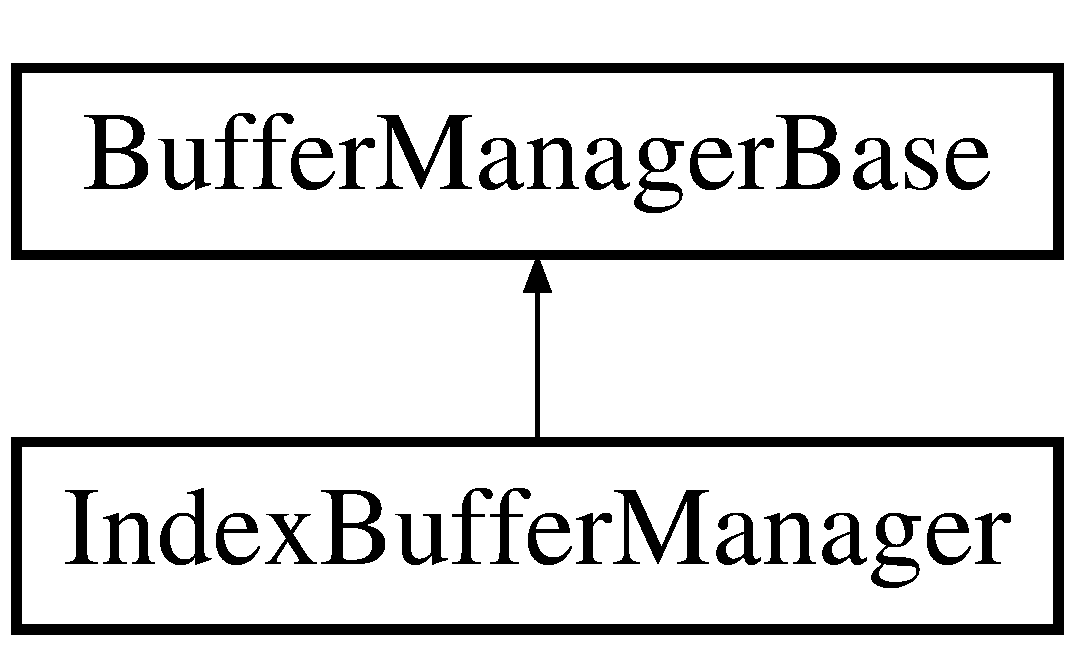
\includegraphics[height=2.000000cm]{d9/d4b/class_index_buffer_manager}
\end{center}
\end{figure}
\subsection*{Public Member Functions}
\begin{DoxyCompactItemize}
\item 
\mbox{\hyperlink{stdafx_8h_a8ee2d990c5dfba7794dd2b60741d7722}{D3\+D\+E\+N\+G\+I\+N\+E\+\_\+\+A\+PI}} \mbox{\hyperlink{class_index_buffer_manager_a58352b8fc2032a4e29faed7fbe249ea0}{Index\+Buffer\+Manager}} (std\+::shared\+\_\+ptr$<$ std\+::vector$<$ unsigned int $>$$>$ vertices, const std\+::shared\+\_\+ptr$<$ \mbox{\hyperlink{class_d_x_1_1_device_resources}{D\+X\+::\+Device\+Resources}} $>$ device\+Resources, const std\+::shared\+\_\+ptr$<$ \mbox{\hyperlink{class_command_list_manager}{Command\+List\+Manager}} $>$ command\+List\+Manager)
\begin{DoxyCompactList}\small\item\em Construct a new Index Buffer Manager\+:\+: Index Buffer Manager object. \end{DoxyCompactList}\item 
\mbox{\hyperlink{stdafx_8h_a8ee2d990c5dfba7794dd2b60741d7722}{D3\+D\+E\+N\+G\+I\+N\+E\+\_\+\+A\+PI}} \mbox{\hyperlink{class_index_buffer_manager_af5f43b500ab9536bb2b598e94b7951b9}{$\sim$\+Index\+Buffer\+Manager}} ()
\begin{DoxyCompactList}\small\item\em Destroy the Index Buffer Manager\+:\+: Index Buffer Manager object. \end{DoxyCompactList}\item 
\mbox{\hyperlink{stdafx_8h_a8ee2d990c5dfba7794dd2b60741d7722}{D3\+D\+E\+N\+G\+I\+N\+E\+\_\+\+A\+PI}} D3\+D12\+\_\+\+I\+N\+D\+E\+X\+\_\+\+B\+U\+F\+F\+E\+R\+\_\+\+V\+I\+EW \mbox{\hyperlink{class_index_buffer_manager_a061f4f1d39af54908dbd31eb9afa03fa}{Create\+Index\+Buffer\+View}} ()
\begin{DoxyCompactList}\small\item\em creates the index bufer view which can be used by the command list to add it to rendering \end{DoxyCompactList}\end{DoxyCompactItemize}
\subsection*{Private Attributes}
\begin{DoxyCompactItemize}
\item 
std\+::shared\+\_\+ptr$<$ std\+::vector$<$ unsigned int $>$ $>$ \mbox{\hyperlink{class_index_buffer_manager_ade308a27ee394d550f91c919411df37b}{m\+\_\+indices}}
\item 
size\+\_\+t \mbox{\hyperlink{class_index_buffer_manager_ae21d575fdd0af30b3050c5747f20ad66}{m\+\_\+indices\+Size}}
\begin{DoxyCompactList}\small\item\em The index data. \end{DoxyCompactList}\end{DoxyCompactItemize}


\subsection{Detailed Description}


Definition at line 5 of file Index\+Buffer\+Manager.\+h.



\subsection{Constructor \& Destructor Documentation}
\mbox{\Hypertarget{class_index_buffer_manager_a58352b8fc2032a4e29faed7fbe249ea0}\label{class_index_buffer_manager_a58352b8fc2032a4e29faed7fbe249ea0}} 
\index{Index\+Buffer\+Manager@{Index\+Buffer\+Manager}!Index\+Buffer\+Manager@{Index\+Buffer\+Manager}}
\index{Index\+Buffer\+Manager@{Index\+Buffer\+Manager}!Index\+Buffer\+Manager@{Index\+Buffer\+Manager}}
\subsubsection{\texorpdfstring{Index\+Buffer\+Manager()}{IndexBufferManager()}}
{\footnotesize\ttfamily Index\+Buffer\+Manager\+::\+Index\+Buffer\+Manager (\begin{DoxyParamCaption}\item[{std\+::shared\+\_\+ptr$<$ std\+::vector$<$ unsigned int $>$$>$}]{indices,  }\item[{const std\+::shared\+\_\+ptr$<$ \mbox{\hyperlink{class_d_x_1_1_device_resources}{D\+X\+::\+Device\+Resources}} $>$}]{device\+Resources,  }\item[{const std\+::shared\+\_\+ptr$<$ \mbox{\hyperlink{class_command_list_manager}{Command\+List\+Manager}} $>$}]{command\+List\+Manager }\end{DoxyParamCaption})}



Construct a new Index Buffer Manager\+:\+: Index Buffer Manager object. 


\begin{DoxyParams}{Parameters}
{\em indices} & the vector of indices to be added to the buffer \\
\hline
{\em device\+Resources} & \\
\hline
{\em command\+List\+Manager} & \\
\hline
\end{DoxyParams}


Definition at line 11 of file Index\+Buffer\+Manager.\+cpp.


\begin{DoxyCode}
13                                                                 :
14     \mbox{\hyperlink{class_buffer_manager_base_a9cec2f80ae72dc972ef6d18ab075ab6c}{BufferManagerBase}}(indices->size() * \textcolor{keyword}{sizeof}(\textcolor{keywordtype}{unsigned} int),
15         reinterpret\_cast<BYTE*>(indices->data()),
16         D3D12\_RESOURCE\_STATE\_INDEX\_BUFFER,
17         deviceResources,
18         commandListManager),
19     \mbox{\hyperlink{class_index_buffer_manager_ade308a27ee394d550f91c919411df37b}{m\_indices}}(indices)
20 \{
21     \mbox{\hyperlink{class_index_buffer_manager_ae21d575fdd0af30b3050c5747f20ad66}{m\_indicesSize}} = \mbox{\hyperlink{class_index_buffer_manager_ade308a27ee394d550f91c919411df37b}{m\_indices}}->size();
22 \}
\end{DoxyCode}
\mbox{\Hypertarget{class_index_buffer_manager_af5f43b500ab9536bb2b598e94b7951b9}\label{class_index_buffer_manager_af5f43b500ab9536bb2b598e94b7951b9}} 
\index{Index\+Buffer\+Manager@{Index\+Buffer\+Manager}!````~Index\+Buffer\+Manager@{$\sim$\+Index\+Buffer\+Manager}}
\index{````~Index\+Buffer\+Manager@{$\sim$\+Index\+Buffer\+Manager}!Index\+Buffer\+Manager@{Index\+Buffer\+Manager}}
\subsubsection{\texorpdfstring{$\sim$\+Index\+Buffer\+Manager()}{~IndexBufferManager()}}
{\footnotesize\ttfamily Index\+Buffer\+Manager\+::$\sim$\+Index\+Buffer\+Manager (\begin{DoxyParamCaption}{ }\end{DoxyParamCaption})}



Destroy the Index Buffer Manager\+:\+: Index Buffer Manager object. 



Definition at line 27 of file Index\+Buffer\+Manager.\+cpp.


\begin{DoxyCode}
28 \{
29     \mbox{\hyperlink{class_index_buffer_manager_ade308a27ee394d550f91c919411df37b}{m\_indices}}->clear();
30 \}
\end{DoxyCode}


\subsection{Member Function Documentation}
\mbox{\Hypertarget{class_index_buffer_manager_a061f4f1d39af54908dbd31eb9afa03fa}\label{class_index_buffer_manager_a061f4f1d39af54908dbd31eb9afa03fa}} 
\index{Index\+Buffer\+Manager@{Index\+Buffer\+Manager}!Create\+Index\+Buffer\+View@{Create\+Index\+Buffer\+View}}
\index{Create\+Index\+Buffer\+View@{Create\+Index\+Buffer\+View}!Index\+Buffer\+Manager@{Index\+Buffer\+Manager}}
\subsubsection{\texorpdfstring{Create\+Index\+Buffer\+View()}{CreateIndexBufferView()}}
{\footnotesize\ttfamily D3\+D12\+\_\+\+I\+N\+D\+E\+X\+\_\+\+B\+U\+F\+F\+E\+R\+\_\+\+V\+I\+EW Index\+Buffer\+Manager\+::\+Create\+Index\+Buffer\+View (\begin{DoxyParamCaption}{ }\end{DoxyParamCaption})}



creates the index bufer view which can be used by the command list to add it to rendering 

\begin{DoxyReturn}{Returns}
D3\+D12\+\_\+\+I\+N\+D\+E\+X\+\_\+\+B\+U\+F\+F\+E\+R\+\_\+\+V\+I\+EW the view 
\end{DoxyReturn}


Definition at line 36 of file Index\+Buffer\+Manager.\+cpp.


\begin{DoxyCode}
37 \{
38     \textcolor{comment}{//describe and create index buffer view}
39     D3D12\_INDEX\_BUFFER\_VIEW vertexBufferView;
40     vertexBufferView.BufferLocation = \mbox{\hyperlink{class_buffer_manager_base_afa03f652ef76e70618f7f112b7da48c5}{GetResource}}()->GetGPUVirtualAddress();
41     vertexBufferView.Format = DXGI\_FORMAT\_R32\_UINT;
42     vertexBufferView.SizeInBytes = \textcolor{keyword}{sizeof}(\textcolor{keywordtype}{unsigned} int) * \mbox{\hyperlink{class_index_buffer_manager_ae21d575fdd0af30b3050c5747f20ad66}{m\_indicesSize}};
43 
44     \textcolor{keywordflow}{return} vertexBufferView;
45 \}
\end{DoxyCode}


\subsection{Member Data Documentation}
\mbox{\Hypertarget{class_index_buffer_manager_ade308a27ee394d550f91c919411df37b}\label{class_index_buffer_manager_ade308a27ee394d550f91c919411df37b}} 
\index{Index\+Buffer\+Manager@{Index\+Buffer\+Manager}!m\+\_\+indices@{m\+\_\+indices}}
\index{m\+\_\+indices@{m\+\_\+indices}!Index\+Buffer\+Manager@{Index\+Buffer\+Manager}}
\subsubsection{\texorpdfstring{m\+\_\+indices}{m\_indices}}
{\footnotesize\ttfamily std\+::shared\+\_\+ptr$<$std\+::vector$<$unsigned int$>$ $>$ Index\+Buffer\+Manager\+::m\+\_\+indices\hspace{0.3cm}{\ttfamily [private]}}



Definition at line 13 of file Index\+Buffer\+Manager.\+h.

\mbox{\Hypertarget{class_index_buffer_manager_ae21d575fdd0af30b3050c5747f20ad66}\label{class_index_buffer_manager_ae21d575fdd0af30b3050c5747f20ad66}} 
\index{Index\+Buffer\+Manager@{Index\+Buffer\+Manager}!m\+\_\+indices\+Size@{m\+\_\+indices\+Size}}
\index{m\+\_\+indices\+Size@{m\+\_\+indices\+Size}!Index\+Buffer\+Manager@{Index\+Buffer\+Manager}}
\subsubsection{\texorpdfstring{m\+\_\+indices\+Size}{m\_indicesSize}}
{\footnotesize\ttfamily size\+\_\+t Index\+Buffer\+Manager\+::m\+\_\+indices\+Size\hspace{0.3cm}{\ttfamily [private]}}



The index data. 



Definition at line 14 of file Index\+Buffer\+Manager.\+h.



The documentation for this class was generated from the following files\+:\begin{DoxyCompactItemize}
\item 
D3d\+Engine/\mbox{\hyperlink{_index_buffer_manager_8h}{Index\+Buffer\+Manager.\+h}}\item 
D3d\+Engine/\mbox{\hyperlink{_index_buffer_manager_8cpp}{Index\+Buffer\+Manager.\+cpp}}\end{DoxyCompactItemize}

\hypertarget{struct_texture_resource_manager_1_1_loaded_data}{}\section{Texture\+Resource\+Manager\+:\+:Loaded\+Data Struct Reference}
\label{struct_texture_resource_manager_1_1_loaded_data}\index{Texture\+Resource\+Manager\+::\+Loaded\+Data@{Texture\+Resource\+Manager\+::\+Loaded\+Data}}
\subsection*{Public Attributes}
\begin{DoxyCompactItemize}
\item 
B\+Y\+TE $\ast$ \mbox{\hyperlink{struct_texture_resource_manager_1_1_loaded_data_ab8f8bbcc8db59da66d27455d98fec3d0}{texture\+Data}}
\item 
int \mbox{\hyperlink{struct_texture_resource_manager_1_1_loaded_data_a606406cf7042b156ccaaff5c718f3d4a}{image\+Bytes\+Per\+Row}}
\end{DoxyCompactItemize}


\subsection{Detailed Description}


Definition at line 16 of file Texture\+Resource\+Manager.\+h.



\subsection{Member Data Documentation}
\mbox{\Hypertarget{struct_texture_resource_manager_1_1_loaded_data_a606406cf7042b156ccaaff5c718f3d4a}\label{struct_texture_resource_manager_1_1_loaded_data_a606406cf7042b156ccaaff5c718f3d4a}} 
\index{Texture\+Resource\+Manager\+::\+Loaded\+Data@{Texture\+Resource\+Manager\+::\+Loaded\+Data}!image\+Bytes\+Per\+Row@{image\+Bytes\+Per\+Row}}
\index{image\+Bytes\+Per\+Row@{image\+Bytes\+Per\+Row}!Texture\+Resource\+Manager\+::\+Loaded\+Data@{Texture\+Resource\+Manager\+::\+Loaded\+Data}}
\subsubsection{\texorpdfstring{image\+Bytes\+Per\+Row}{imageBytesPerRow}}
{\footnotesize\ttfamily int Texture\+Resource\+Manager\+::\+Loaded\+Data\+::image\+Bytes\+Per\+Row}



Definition at line 19 of file Texture\+Resource\+Manager.\+h.

\mbox{\Hypertarget{struct_texture_resource_manager_1_1_loaded_data_ab8f8bbcc8db59da66d27455d98fec3d0}\label{struct_texture_resource_manager_1_1_loaded_data_ab8f8bbcc8db59da66d27455d98fec3d0}} 
\index{Texture\+Resource\+Manager\+::\+Loaded\+Data@{Texture\+Resource\+Manager\+::\+Loaded\+Data}!texture\+Data@{texture\+Data}}
\index{texture\+Data@{texture\+Data}!Texture\+Resource\+Manager\+::\+Loaded\+Data@{Texture\+Resource\+Manager\+::\+Loaded\+Data}}
\subsubsection{\texorpdfstring{texture\+Data}{textureData}}
{\footnotesize\ttfamily B\+Y\+TE$\ast$ Texture\+Resource\+Manager\+::\+Loaded\+Data\+::texture\+Data}



Definition at line 18 of file Texture\+Resource\+Manager.\+h.



The documentation for this struct was generated from the following file\+:\begin{DoxyCompactItemize}
\item 
D3d\+Engine/\mbox{\hyperlink{_texture_resource_manager_8h}{Texture\+Resource\+Manager.\+h}}\end{DoxyCompactItemize}

\hypertarget{class_model_loader}{}\section{Model\+Loader Class Reference}
\label{class_model_loader}\index{Model\+Loader@{Model\+Loader}}


deprecated, for use only when coxl loader not working  




{\ttfamily \#include $<$Model\+Loader.\+h$>$}

\subsection*{Public Member Functions}
\begin{DoxyCompactItemize}
\item 
\mbox{\hyperlink{stdafx_8h_a8ee2d990c5dfba7794dd2b60741d7722}{D3\+D\+E\+N\+G\+I\+N\+E\+\_\+\+A\+PI}} \mbox{\hyperlink{struct_structures_1_1_vertices_indices}{Structures\+::\+Vertices\+Indices}} \mbox{\hyperlink{class_model_loader_aa70efbdc2fff6bf8208fcc76cfd4a464}{Load\+Model\+From\+File}} (std\+::string file\+Name)
\begin{DoxyCompactList}\small\item\em The general rule is that you should not use this as it is for debug cases only (incase the C\+O\+XL loader fails or is broken) \end{DoxyCompactList}\end{DoxyCompactItemize}
\subsection*{Private Member Functions}
\begin{DoxyCompactItemize}
\item 
X\+M\+M\+A\+T\+R\+IX \mbox{\hyperlink{class_model_loader_aca3f1bef5b2ab890212784626559482c}{get\+Parent\+Trans}} (X\+M\+M\+A\+T\+R\+IX, ai\+Node $\ast$node)
\item 
void \mbox{\hyperlink{class_model_loader_ae809d56b350b003306b484c3bbc1b5e3}{Init\+From\+Scene}} (const ai\+Scene $\ast$scene)
\item 
void \mbox{\hyperlink{class_model_loader_afebdf188f92f87cdcefdee2b4b474727}{Load\+Animations}} (const ai\+Scene $\ast$scene)
\item 
void \mbox{\hyperlink{class_model_loader_a77713e17f817861d8b6b3b166248abe7}{Load\+Bones}} (const ai\+Scene $\ast$scene, const int i)
\item 
std\+::vector$<$ unsigned $>$ \mbox{\hyperlink{class_model_loader_aade9d7c2c0a8a13800700ee3b4b930ef}{load\+Indices}} (const ai\+Scene $\ast$scene, const int i)
\item 
std\+::vector$<$ \mbox{\hyperlink{struct_structures_1_1_vertex_tex_coord_normal_bones}{Structures\+::\+Vertex\+Tex\+Coord\+Normal\+Bones}} $>$ \mbox{\hyperlink{class_model_loader_a90e1f853324d4aee05ba5db140aa974d}{load\+Vertices}} (const ai\+Scene $\ast$scene, const int i)
\item 
int \mbox{\hyperlink{class_model_loader_a5356ad9c0e77c4b5142c1c1400b01048}{Find\+Bone\+With\+Keys}} (std\+::vector$<$ \mbox{\hyperlink{struct_structures_1_1_anim_bone}{Structures\+::\+Anim\+Bone}} $>$ bones, std\+::string name)
\item 
std\+::vector$<$ \mbox{\hyperlink{struct_structures_1_1_anim_bone}{Structures\+::\+Anim\+Bone}} $>$ \mbox{\hyperlink{class_model_loader_afabe255fd413f08ac9939e786f26aee4}{Get\+Nodes}} (ai\+Node $\ast$node, std\+::vector$<$ \mbox{\hyperlink{struct_structures_1_1_anim_bone}{Structures\+::\+Anim\+Bone}} $>$ list)
\item 
X\+M\+M\+A\+T\+R\+IX \mbox{\hyperlink{class_model_loader_ab142e176c572ea327518f01fb2f0630b}{ai\+To\+Xmmatrix}} (ai\+Matrix4x4 mat)
\end{DoxyCompactItemize}
\subsection*{Private Attributes}
\begin{DoxyCompactItemize}
\item 
std\+::vector$<$ \mbox{\hyperlink{struct_structures_1_1_vertex_tex_coord_normal_bones}{Structures\+::\+Vertex\+Tex\+Coord\+Normal\+Bones}} $>$ \mbox{\hyperlink{class_model_loader_ac87b9662dae9c00b140bc90c30c088ee}{m\+\_\+vertices}}
\item 
std\+::vector$<$ unsigned $>$ \mbox{\hyperlink{class_model_loader_a6d63371db7677b60c2c000f23c7fb8f6}{m\+\_\+indices}}
\item 
std\+::vector$<$ \mbox{\hyperlink{struct_structures_1_1_animation}{Structures\+::\+Animation}} $>$ \mbox{\hyperlink{class_model_loader_a2b9cf4d8fe3432ddc656651057c78860}{m\+\_\+animations}}
\end{DoxyCompactItemize}


\subsection{Detailed Description}
deprecated, for use only when coxl loader not working 

Definition at line 10 of file Model\+Loader.\+h.



\subsection{Member Function Documentation}
\mbox{\Hypertarget{class_model_loader_ab142e176c572ea327518f01fb2f0630b}\label{class_model_loader_ab142e176c572ea327518f01fb2f0630b}} 
\index{Model\+Loader@{Model\+Loader}!ai\+To\+Xmmatrix@{ai\+To\+Xmmatrix}}
\index{ai\+To\+Xmmatrix@{ai\+To\+Xmmatrix}!Model\+Loader@{Model\+Loader}}
\subsubsection{\texorpdfstring{ai\+To\+Xmmatrix()}{aiToXmmatrix()}}
{\footnotesize\ttfamily X\+M\+M\+A\+T\+R\+IX Model\+Loader\+::ai\+To\+Xmmatrix (\begin{DoxyParamCaption}\item[{ai\+Matrix4x4}]{mat }\end{DoxyParamCaption})\hspace{0.3cm}{\ttfamily [private]}}



Definition at line 218 of file Model\+Loader.\+cpp.


\begin{DoxyCode}
219 \{
220     \textcolor{keyword}{auto} matrix = mat;
221     \textcolor{keyword}{auto} trans = XMFLOAT4X4(
222         matrix.a1, matrix.a2, matrix.a3, matrix.a4,
223         matrix.b1, matrix.b2, matrix.b3, matrix.b4,
224         matrix.c1, matrix.c2, matrix.c3, matrix.c4,
225         matrix.d1, matrix.d2, matrix.d3, matrix.d4
226     );
227     \textcolor{keywordflow}{return} XMLoadFloat4x4(&trans);
228 \}
\end{DoxyCode}
\mbox{\Hypertarget{class_model_loader_a5356ad9c0e77c4b5142c1c1400b01048}\label{class_model_loader_a5356ad9c0e77c4b5142c1c1400b01048}} 
\index{Model\+Loader@{Model\+Loader}!Find\+Bone\+With\+Keys@{Find\+Bone\+With\+Keys}}
\index{Find\+Bone\+With\+Keys@{Find\+Bone\+With\+Keys}!Model\+Loader@{Model\+Loader}}
\subsubsection{\texorpdfstring{Find\+Bone\+With\+Keys()}{FindBoneWithKeys()}}
{\footnotesize\ttfamily int Model\+Loader\+::\+Find\+Bone\+With\+Keys (\begin{DoxyParamCaption}\item[{std\+::vector$<$ \mbox{\hyperlink{struct_structures_1_1_anim_bone}{Structures\+::\+Anim\+Bone}} $>$}]{bones,  }\item[{std\+::string}]{name }\end{DoxyParamCaption})\hspace{0.3cm}{\ttfamily [private]}}



Definition at line 187 of file Model\+Loader.\+cpp.


\begin{DoxyCode}
188 \{
189     \textcolor{keywordflow}{for} (\textcolor{keyword}{auto} bone = 0; bone < bones.size(); bone++)
190     \{
191         \textcolor{keywordflow}{if} (bones[bone].name == name)
192         \{
193             \textcolor{keywordflow}{return} bone;
194         \}
195     \}
196     \textcolor{keywordflow}{return} -1;
197 \}
\end{DoxyCode}
\mbox{\Hypertarget{class_model_loader_afabe255fd413f08ac9939e786f26aee4}\label{class_model_loader_afabe255fd413f08ac9939e786f26aee4}} 
\index{Model\+Loader@{Model\+Loader}!Get\+Nodes@{Get\+Nodes}}
\index{Get\+Nodes@{Get\+Nodes}!Model\+Loader@{Model\+Loader}}
\subsubsection{\texorpdfstring{Get\+Nodes()}{GetNodes()}}
{\footnotesize\ttfamily std\+::vector$<$ \mbox{\hyperlink{struct_structures_1_1_anim_bone}{Structures\+::\+Anim\+Bone}} $>$ Model\+Loader\+::\+Get\+Nodes (\begin{DoxyParamCaption}\item[{ai\+Node $\ast$}]{node,  }\item[{std\+::vector$<$ \mbox{\hyperlink{struct_structures_1_1_anim_bone}{Structures\+::\+Anim\+Bone}} $>$}]{list }\end{DoxyParamCaption})\hspace{0.3cm}{\ttfamily [private]}}



Definition at line 199 of file Model\+Loader.\+cpp.


\begin{DoxyCode}
199                                                                                                       \{
200     \textcolor{keywordflow}{if} (node->mNumChildren > 0) \{
201         \textcolor{keywordflow}{for} (\textcolor{keyword}{auto} i = 0; i < node->mNumChildren; i++) \{
202             \textcolor{keyword}{auto} childBoneId = \mbox{\hyperlink{class_model_loader_a5356ad9c0e77c4b5142c1c1400b01048}{FindBoneWithKeys}}(list, node->mChildren[i]->mName.data);
203             \textcolor{keyword}{auto} childTransform = list[childBoneId];
204             \textcolor{keyword}{auto} parentTransform = list[\mbox{\hyperlink{class_model_loader_a5356ad9c0e77c4b5142c1c1400b01048}{FindBoneWithKeys}}(list, node->mName.data)];
205             \textcolor{keyword}{auto} trans = \mbox{\hyperlink{class_model_loader_ab142e176c572ea327518f01fb2f0630b}{aiToXmmatrix}}(node->mChildren[i]->mTransformation);
206             \textcolor{keywordflow}{for} (\textcolor{keyword}{auto} i = 0; i < childTransform.transforms.size(); i++) \{
207                 childTransform.transforms[i] = (childTransform.transforms[i] * parentTransform.transforms[i
      ]);
208                 \textcolor{keyword}{auto} offset = childTransform.offsetMatrix;
209                 childTransform.finalTransforms.push\_back(XMMatrixTranspose(offset) * ((childTransform.
      transforms[i])));
210             \}
211             list[childBoneId] = childTransform;
212             list = \mbox{\hyperlink{class_model_loader_afabe255fd413f08ac9939e786f26aee4}{GetNodes}}(node->mChildren[i], list);
213         \}
214     \}
215     \textcolor{keywordflow}{return} list;
216 \}
\end{DoxyCode}
\mbox{\Hypertarget{class_model_loader_aca3f1bef5b2ab890212784626559482c}\label{class_model_loader_aca3f1bef5b2ab890212784626559482c}} 
\index{Model\+Loader@{Model\+Loader}!get\+Parent\+Trans@{get\+Parent\+Trans}}
\index{get\+Parent\+Trans@{get\+Parent\+Trans}!Model\+Loader@{Model\+Loader}}
\subsubsection{\texorpdfstring{get\+Parent\+Trans()}{getParentTrans()}}
{\footnotesize\ttfamily X\+M\+M\+A\+T\+R\+IX Model\+Loader\+::get\+Parent\+Trans (\begin{DoxyParamCaption}\item[{X\+M\+M\+A\+T\+R\+IX}]{mat,  }\item[{ai\+Node $\ast$}]{node }\end{DoxyParamCaption})\hspace{0.3cm}{\ttfamily [private]}}



Definition at line 36 of file Model\+Loader.\+cpp.


\begin{DoxyCode}
37 \{
38     \textcolor{keywordflow}{if} (node->mParent) \{
39         \textcolor{keyword}{auto} matrix = node->mParent->mTransformation;
40         \textcolor{keyword}{auto} trans = XMFLOAT4X4(
41             matrix.a1, matrix.a2, matrix.a3, matrix.a4,
42             matrix.b1, matrix.b2, matrix.b3, matrix.b4,
43             matrix.c1, matrix.c2, matrix.c3, matrix.c4,
44             matrix.d1, matrix.d2, matrix.d3, matrix.d4
45         );
46 
47         \textcolor{keywordflow}{return} XMLoadFloat4x4(&trans);
48     \}
49     \textcolor{keywordflow}{return} XMMatrixIdentity();
50 \}
\end{DoxyCode}
\mbox{\Hypertarget{class_model_loader_ae809d56b350b003306b484c3bbc1b5e3}\label{class_model_loader_ae809d56b350b003306b484c3bbc1b5e3}} 
\index{Model\+Loader@{Model\+Loader}!Init\+From\+Scene@{Init\+From\+Scene}}
\index{Init\+From\+Scene@{Init\+From\+Scene}!Model\+Loader@{Model\+Loader}}
\subsubsection{\texorpdfstring{Init\+From\+Scene()}{InitFromScene()}}
{\footnotesize\ttfamily void Model\+Loader\+::\+Init\+From\+Scene (\begin{DoxyParamCaption}\item[{const ai\+Scene $\ast$}]{scene }\end{DoxyParamCaption})\hspace{0.3cm}{\ttfamily [private]}}



Definition at line 52 of file Model\+Loader.\+cpp.


\begin{DoxyCode}
53 \{
54     \mbox{\hyperlink{class_model_loader_afebdf188f92f87cdcefdee2b4b474727}{LoadAnimations}}(scene);
55     \textcolor{keywordflow}{for} (\textcolor{keyword}{auto} i = 0; i < scene->mNumMeshes; i++) \{
56         \mbox{\hyperlink{class_model_loader_ac87b9662dae9c00b140bc90c30c088ee}{m\_vertices}} = \mbox{\hyperlink{class_model_loader_a90e1f853324d4aee05ba5db140aa974d}{loadVertices}}(scene, i);
57         \mbox{\hyperlink{class_model_loader_a6d63371db7677b60c2c000f23c7fb8f6}{m\_indices}} = \mbox{\hyperlink{class_model_loader_aade9d7c2c0a8a13800700ee3b4b930ef}{loadIndices}}(scene, i);
58         \mbox{\hyperlink{class_model_loader_a77713e17f817861d8b6b3b166248abe7}{LoadBones}}(scene, i);
59     \}
60 \}
\end{DoxyCode}
\mbox{\Hypertarget{class_model_loader_afebdf188f92f87cdcefdee2b4b474727}\label{class_model_loader_afebdf188f92f87cdcefdee2b4b474727}} 
\index{Model\+Loader@{Model\+Loader}!Load\+Animations@{Load\+Animations}}
\index{Load\+Animations@{Load\+Animations}!Model\+Loader@{Model\+Loader}}
\subsubsection{\texorpdfstring{Load\+Animations()}{LoadAnimations()}}
{\footnotesize\ttfamily void Model\+Loader\+::\+Load\+Animations (\begin{DoxyParamCaption}\item[{const ai\+Scene $\ast$}]{scene }\end{DoxyParamCaption})\hspace{0.3cm}{\ttfamily [private]}}



Definition at line 62 of file Model\+Loader.\+cpp.


\begin{DoxyCode}
63 \{
64     \textcolor{keywordflow}{for} (\textcolor{keyword}{auto} i = 0; i < scene->mNumAnimations; i++) \{
65         \textcolor{keyword}{auto} animation = \mbox{\hyperlink{struct_structures_1_1_animation}{Structures::Animation}}\{\};
66 
67         animation.\mbox{\hyperlink{struct_structures_1_1_animation_a6726c126620084018287d0f9211db2b8}{bonesWithKeys}} = std::vector<Structures::AnimBone>();
68         \textcolor{keywordflow}{for} (\textcolor{keyword}{auto} j = 0; j < scene->mAnimations[i]->mNumChannels; j++) \{
69             \textcolor{keyword}{auto} channel = scene->mAnimations[i]->mChannels[j];
70             \textcolor{keyword}{auto} transforms = std::vector<XMMATRIX>();
71             \textcolor{keywordflow}{for} (\textcolor{keyword}{auto} key = 0; key < channel->mNumPositionKeys; key++) \{
72                 \textcolor{keyword}{auto} translation = XMVectorSet(
73                     channel->mPositionKeys[key].mValue.x,
74                     channel->mPositionKeys[key].mValue.y,
75                     channel->mPositionKeys[key].mValue.z, 0);
76                 \textcolor{keyword}{auto} rotation = XMVectorSet(
77                     channel->mRotationKeys[key].mValue.x,
78                     channel->mRotationKeys[key].mValue.y,
79                     channel->mRotationKeys[key].mValue.z,
80                     channel->mRotationKeys[key].mValue.w);
81                 \textcolor{keyword}{auto} scaling = XMVectorSet(
82                     channel->mScalingKeys[key].mValue.x,
83                     channel->mScalingKeys[key].mValue.y,
84                     channel->mScalingKeys[key].mValue.z, 1);
85                 \textcolor{keyword}{auto} zero = XMVectorSet(0, 0, 0, 1);
86 
87                 \textcolor{keyword}{auto} transform = XMMatrixAffineTransformation(scaling, zero, rotation, translation);
88                 transforms.push\_back(transform);
89             \}
90             \textcolor{keywordflow}{if} (std::string(channel->mNodeName.data) == \textcolor{stringliteral}{"Cube"}) \{
91                 \textcolor{keywordflow}{continue};
92             \}
93             \textcolor{keyword}{auto} animBone = \mbox{\hyperlink{struct_structures_1_1_anim_bone}{Structures::AnimBone}}\{ channel->mNodeName.data, transforms \}
      ;
94             animation.bonesWithKeys.push\_back(animBone);
95             animation.frameCount = scene->mAnimations[i]->mDuration * 24;
96         \}
97         \mbox{\hyperlink{class_model_loader_a2b9cf4d8fe3432ddc656651057c78860}{m\_animations}}.push\_back(animation);
98     \}
99 \}
\end{DoxyCode}
\mbox{\Hypertarget{class_model_loader_a77713e17f817861d8b6b3b166248abe7}\label{class_model_loader_a77713e17f817861d8b6b3b166248abe7}} 
\index{Model\+Loader@{Model\+Loader}!Load\+Bones@{Load\+Bones}}
\index{Load\+Bones@{Load\+Bones}!Model\+Loader@{Model\+Loader}}
\subsubsection{\texorpdfstring{Load\+Bones()}{LoadBones()}}
{\footnotesize\ttfamily void Model\+Loader\+::\+Load\+Bones (\begin{DoxyParamCaption}\item[{const ai\+Scene $\ast$}]{scene,  }\item[{const int}]{i }\end{DoxyParamCaption})\hspace{0.3cm}{\ttfamily [private]}}



Definition at line 101 of file Model\+Loader.\+cpp.


\begin{DoxyCode}
102 \{
103     \textcolor{keywordflow}{for} (\textcolor{keyword}{auto} x = 0; x < scene->mMeshes[i]->mNumBones; x++)
104     \{
105         \textcolor{keywordflow}{for} (\textcolor{keyword}{auto} &animation : \mbox{\hyperlink{class_model_loader_a2b9cf4d8fe3432ddc656651057c78860}{m\_animations}})
106         \{
107             \textcolor{keywordflow}{for} (\textcolor{keyword}{auto} z = 0; z < \mbox{\hyperlink{class_model_loader_a2b9cf4d8fe3432ddc656651057c78860}{m\_animations}}[0].bonesWithKeys.size(); z++)
108             \{
109                 \textcolor{keywordflow}{if} (animation.bonesWithKeys[z].name == std::string(scene->mMeshes[i]->mBones[x]->mName.data
      ))
110                 \{
111                     \textcolor{keyword}{const} \textcolor{keyword}{auto} mat = scene->mMeshes[i]->mBones[x]->mOffsetMatrix;
112                     animation.bonesWithKeys[z].offsetMatrix = \mbox{\hyperlink{class_model_loader_ab142e176c572ea327518f01fb2f0630b}{aiToXmmatrix}}(mat);
113                     \textcolor{keywordflow}{for} (\textcolor{keyword}{auto} y = 0; y < scene->mMeshes[i]->mBones[x]->mNumWeights; y++)
114                     \{
115                         \mbox{\hyperlink{class_model_loader_ac87b9662dae9c00b140bc90c30c088ee}{m\_vertices}}[scene->mMeshes[i]->mBones[x]->mWeights[y].mVertexId].bones.
      push\_back(\{
116                             \textcolor{keyword}{static\_cast<}UINT\textcolor{keyword}{>}(z), scene->mMeshes[i]->mBones[x]->mWeights[y].mWeight \});
117                     \}
118                     \textcolor{keywordflow}{break};
119                 \}
120             \}
121         \}
122     \}
123 
124     \textcolor{keyword}{auto} root = scene->mRootNode;
125     root = root->FindNode(\textcolor{stringliteral}{"Armature"});
126     \textcolor{keywordflow}{for} (\textcolor{keyword}{auto} anim = 0; anim < \mbox{\hyperlink{class_model_loader_a2b9cf4d8fe3432ddc656651057c78860}{m\_animations}}.size(); anim++)
127     \{
128         \textcolor{keywordflow}{for} (\textcolor{keyword}{auto} i = 0; i < root->mNumChildren; i++) \{
129             \textcolor{keyword}{auto} childBoneId = \mbox{\hyperlink{class_model_loader_a5356ad9c0e77c4b5142c1c1400b01048}{FindBoneWithKeys}}(\mbox{\hyperlink{class_model_loader_a2b9cf4d8fe3432ddc656651057c78860}{m\_animations}}[anim].
      bonesWithKeys, root->mChildren[i]->mName.data);
130             \textcolor{keyword}{auto} childTransform = \mbox{\hyperlink{class_model_loader_a2b9cf4d8fe3432ddc656651057c78860}{m\_animations}}[anim].bonesWithKeys[childBoneId];
131             \textcolor{keywordflow}{for} (\textcolor{keyword}{auto} i = 0; i < childTransform.transforms.size(); i++) \{
132                 childTransform.transforms[i] = childTransform.transforms[i];
133                 \textcolor{keyword}{auto} offset = childTransform.offsetMatrix;
134                 childTransform.finalTransforms.push\_back(XMMatrixTranspose(offset) * childTransform.
      transforms[i]);
135             \}
136             \mbox{\hyperlink{class_model_loader_a2b9cf4d8fe3432ddc656651057c78860}{m\_animations}}[anim].bonesWithKeys[childBoneId] = childTransform;
137             \mbox{\hyperlink{class_model_loader_a2b9cf4d8fe3432ddc656651057c78860}{m\_animations}}[anim].bonesWithKeys = \mbox{\hyperlink{class_model_loader_afabe255fd413f08ac9939e786f26aee4}{GetNodes}}(root->mChildren[i], 
      \mbox{\hyperlink{class_model_loader_a2b9cf4d8fe3432ddc656651057c78860}{m\_animations}}[anim].bonesWithKeys);
138 
139         \}
140     \}
141 \}
\end{DoxyCode}
\mbox{\Hypertarget{class_model_loader_aade9d7c2c0a8a13800700ee3b4b930ef}\label{class_model_loader_aade9d7c2c0a8a13800700ee3b4b930ef}} 
\index{Model\+Loader@{Model\+Loader}!load\+Indices@{load\+Indices}}
\index{load\+Indices@{load\+Indices}!Model\+Loader@{Model\+Loader}}
\subsubsection{\texorpdfstring{load\+Indices()}{loadIndices()}}
{\footnotesize\ttfamily std\+::vector$<$ unsigned $>$ Model\+Loader\+::load\+Indices (\begin{DoxyParamCaption}\item[{const ai\+Scene $\ast$}]{scene,  }\item[{const int}]{i }\end{DoxyParamCaption})\hspace{0.3cm}{\ttfamily [private]}}



Definition at line 144 of file Model\+Loader.\+cpp.


\begin{DoxyCode}
145 \{
146     std::vector<unsigned> indices = std::vector<unsigned>();
147     \textcolor{keywordflow}{if} (scene->mMeshes[i]->HasFaces())
148     \{
149         \textcolor{keywordflow}{for} (\textcolor{keyword}{auto} j = 0; j < scene->mMeshes[i]->mNumFaces; j++)
150         \{
151             \textcolor{keywordflow}{for} (\textcolor{keyword}{auto} k = 0; k < scene->mMeshes[i]->mFaces[j].mNumIndices; k++)
152             \{
153                 indices.push\_back(scene->mMeshes[i]->mFaces[j].mIndices[k]);
154             \}
155         \}
156     \}
157     std::reverse(indices.begin(), indices.end());
158     \textcolor{keywordflow}{return} indices;
159 \}
\end{DoxyCode}
\mbox{\Hypertarget{class_model_loader_aa70efbdc2fff6bf8208fcc76cfd4a464}\label{class_model_loader_aa70efbdc2fff6bf8208fcc76cfd4a464}} 
\index{Model\+Loader@{Model\+Loader}!Load\+Model\+From\+File@{Load\+Model\+From\+File}}
\index{Load\+Model\+From\+File@{Load\+Model\+From\+File}!Model\+Loader@{Model\+Loader}}
\subsubsection{\texorpdfstring{Load\+Model\+From\+File()}{LoadModelFromFile()}}
{\footnotesize\ttfamily \mbox{\hyperlink{struct_structures_1_1_vertices_indices}{Structures\+::\+Vertices\+Indices}} Model\+Loader\+::\+Load\+Model\+From\+File (\begin{DoxyParamCaption}\item[{std\+::string}]{file\+Name }\end{DoxyParamCaption})}



The general rule is that you should not use this as it is for debug cases only (incase the C\+O\+XL loader fails or is broken) 


\begin{DoxyParams}{Parameters}
{\em file\+Name} & \\
\hline
\end{DoxyParams}
\begin{DoxyReturn}{Returns}
\mbox{\hyperlink{struct_structures_1_1_vertices_indices}{Structures\+::\+Vertices\+Indices}} 
\end{DoxyReturn}


Definition at line 16 of file Model\+Loader.\+cpp.


\begin{DoxyCode}
16                                                                            \{
17 
18     Assimp::Importer importer;
19 
20     \textcolor{keyword}{const} \textcolor{keyword}{auto} scene = importer.ReadFile(fileName, aiProcess\_Triangulate | aiProcess\_JoinIdenticalVertices 
      |
21         aiProcess\_FlipUVs | aiProcess\_GenSmoothNormals);
22 
23     \textcolor{keywordflow}{if} (!scene)
24     \{
25         \textcolor{keywordflow}{return} \{\};
26     \}
27     \textcolor{keyword}{auto} vertices = std::vector<Structures::VertexTexCoordNormalBones>();
28     \textcolor{keyword}{auto} indices = std::vector<unsigned int>();
29     \textcolor{keyword}{auto} vertexCount = 0;
30     \textcolor{keyword}{auto} indexCount = 0;
31 
32     \mbox{\hyperlink{class_model_loader_ae809d56b350b003306b484c3bbc1b5e3}{InitFromScene}}(scene);
33     \textcolor{keywordflow}{return} \{ \mbox{\hyperlink{class_model_loader_ac87b9662dae9c00b140bc90c30c088ee}{m\_vertices}}, \mbox{\hyperlink{class_model_loader_a6d63371db7677b60c2c000f23c7fb8f6}{m\_indices}}, \mbox{\hyperlink{class_model_loader_a2b9cf4d8fe3432ddc656651057c78860}{m\_animations}} \};
34 \}
\end{DoxyCode}
\mbox{\Hypertarget{class_model_loader_a90e1f853324d4aee05ba5db140aa974d}\label{class_model_loader_a90e1f853324d4aee05ba5db140aa974d}} 
\index{Model\+Loader@{Model\+Loader}!load\+Vertices@{load\+Vertices}}
\index{load\+Vertices@{load\+Vertices}!Model\+Loader@{Model\+Loader}}
\subsubsection{\texorpdfstring{load\+Vertices()}{loadVertices()}}
{\footnotesize\ttfamily std\+::vector$<$ \mbox{\hyperlink{struct_structures_1_1_vertex_tex_coord_normal_bones}{Structures\+::\+Vertex\+Tex\+Coord\+Normal\+Bones}} $>$ Model\+Loader\+::load\+Vertices (\begin{DoxyParamCaption}\item[{const ai\+Scene $\ast$}]{scene,  }\item[{const int}]{i }\end{DoxyParamCaption})\hspace{0.3cm}{\ttfamily [private]}}



Definition at line 161 of file Model\+Loader.\+cpp.


\begin{DoxyCode}
162 \{
163     \textcolor{keyword}{auto} vertices = std::vector<Structures::VertexTexCoordNormalBones>();
164     \textcolor{keywordflow}{for} (\textcolor{keyword}{auto} j = 0; j < scene->mMeshes[i]->mNumVertices; j++)
165     \{
166 
167         vertices.push\_back(\{
168             \{
169                 scene->mMeshes[i]->mVertices[j].x,
170                 scene->mMeshes[i]->mVertices[j].y,
171                 scene->mMeshes[i]->mVertices[j].z,
172             \},
173                 \{
174                     scene->mMeshes[i]->mTextureCoords[0][j].x,
175                     scene->mMeshes[i]->mTextureCoords[0][j].y
176                 \},
177                 \{
178                     scene->mMeshes[i]->mNormals[j].x,
179                     scene->mMeshes[i]->mNormals[j].y,
180                     scene->mMeshes[i]->mNormals[j].z,
181                 \},
182             \});
183     \}
184     \textcolor{keywordflow}{return} vertices;
185 \}
\end{DoxyCode}


\subsection{Member Data Documentation}
\mbox{\Hypertarget{class_model_loader_a2b9cf4d8fe3432ddc656651057c78860}\label{class_model_loader_a2b9cf4d8fe3432ddc656651057c78860}} 
\index{Model\+Loader@{Model\+Loader}!m\+\_\+animations@{m\+\_\+animations}}
\index{m\+\_\+animations@{m\+\_\+animations}!Model\+Loader@{Model\+Loader}}
\subsubsection{\texorpdfstring{m\+\_\+animations}{m\_animations}}
{\footnotesize\ttfamily std\+::vector$<$\mbox{\hyperlink{struct_structures_1_1_animation}{Structures\+::\+Animation}}$>$ Model\+Loader\+::m\+\_\+animations\hspace{0.3cm}{\ttfamily [private]}}



Definition at line 28 of file Model\+Loader.\+h.

\mbox{\Hypertarget{class_model_loader_a6d63371db7677b60c2c000f23c7fb8f6}\label{class_model_loader_a6d63371db7677b60c2c000f23c7fb8f6}} 
\index{Model\+Loader@{Model\+Loader}!m\+\_\+indices@{m\+\_\+indices}}
\index{m\+\_\+indices@{m\+\_\+indices}!Model\+Loader@{Model\+Loader}}
\subsubsection{\texorpdfstring{m\+\_\+indices}{m\_indices}}
{\footnotesize\ttfamily std\+::vector$<$unsigned$>$ Model\+Loader\+::m\+\_\+indices\hspace{0.3cm}{\ttfamily [private]}}



Definition at line 27 of file Model\+Loader.\+h.

\mbox{\Hypertarget{class_model_loader_ac87b9662dae9c00b140bc90c30c088ee}\label{class_model_loader_ac87b9662dae9c00b140bc90c30c088ee}} 
\index{Model\+Loader@{Model\+Loader}!m\+\_\+vertices@{m\+\_\+vertices}}
\index{m\+\_\+vertices@{m\+\_\+vertices}!Model\+Loader@{Model\+Loader}}
\subsubsection{\texorpdfstring{m\+\_\+vertices}{m\_vertices}}
{\footnotesize\ttfamily std\+::vector$<$\mbox{\hyperlink{struct_structures_1_1_vertex_tex_coord_normal_bones}{Structures\+::\+Vertex\+Tex\+Coord\+Normal\+Bones}}$>$ Model\+Loader\+::m\+\_\+vertices\hspace{0.3cm}{\ttfamily [private]}}



Definition at line 26 of file Model\+Loader.\+h.



The documentation for this class was generated from the following files\+:\begin{DoxyCompactItemize}
\item 
D3d\+Engine/\mbox{\hyperlink{_model_loader_8h}{Model\+Loader.\+h}}\item 
D3d\+Engine/\mbox{\hyperlink{_model_loader_8cpp}{Model\+Loader.\+cpp}}\end{DoxyCompactItemize}

\hypertarget{struct_structures_1_1_model_view_projection_constant_buffer}{}\section{Structures\+:\+:Model\+View\+Projection\+Constant\+Buffer Struct Reference}
\label{struct_structures_1_1_model_view_projection_constant_buffer}\index{Structures\+::\+Model\+View\+Projection\+Constant\+Buffer@{Structures\+::\+Model\+View\+Projection\+Constant\+Buffer}}


{\ttfamily \#include $<$Structures.\+h$>$}

\subsection*{Public Attributes}
\begin{DoxyCompactItemize}
\item 
Direct\+X\+::\+X\+M\+F\+L\+O\+A\+T4\+X4 \mbox{\hyperlink{struct_structures_1_1_model_view_projection_constant_buffer_adcf32ccfcc0913db019de696791d6333}{model}}
\item 
Direct\+X\+::\+X\+M\+F\+L\+O\+A\+T4\+X4 \mbox{\hyperlink{struct_structures_1_1_model_view_projection_constant_buffer_aede4441ba5f179e090eb088d735ffd34}{view}}
\item 
Direct\+X\+::\+X\+M\+F\+L\+O\+A\+T4\+X4 \mbox{\hyperlink{struct_structures_1_1_model_view_projection_constant_buffer_a515d9a03f96f1d6d35a0713b6fef0386}{projection}}
\end{DoxyCompactItemize}


\subsection{Detailed Description}


Definition at line 89 of file Structures.\+h.



\subsection{Member Data Documentation}
\mbox{\Hypertarget{struct_structures_1_1_model_view_projection_constant_buffer_adcf32ccfcc0913db019de696791d6333}\label{struct_structures_1_1_model_view_projection_constant_buffer_adcf32ccfcc0913db019de696791d6333}} 
\index{Structures\+::\+Model\+View\+Projection\+Constant\+Buffer@{Structures\+::\+Model\+View\+Projection\+Constant\+Buffer}!model@{model}}
\index{model@{model}!Structures\+::\+Model\+View\+Projection\+Constant\+Buffer@{Structures\+::\+Model\+View\+Projection\+Constant\+Buffer}}
\subsubsection{\texorpdfstring{model}{model}}
{\footnotesize\ttfamily Direct\+X\+::\+X\+M\+F\+L\+O\+A\+T4\+X4 Structures\+::\+Model\+View\+Projection\+Constant\+Buffer\+::model}



Definition at line 91 of file Structures.\+h.

\mbox{\Hypertarget{struct_structures_1_1_model_view_projection_constant_buffer_a515d9a03f96f1d6d35a0713b6fef0386}\label{struct_structures_1_1_model_view_projection_constant_buffer_a515d9a03f96f1d6d35a0713b6fef0386}} 
\index{Structures\+::\+Model\+View\+Projection\+Constant\+Buffer@{Structures\+::\+Model\+View\+Projection\+Constant\+Buffer}!projection@{projection}}
\index{projection@{projection}!Structures\+::\+Model\+View\+Projection\+Constant\+Buffer@{Structures\+::\+Model\+View\+Projection\+Constant\+Buffer}}
\subsubsection{\texorpdfstring{projection}{projection}}
{\footnotesize\ttfamily Direct\+X\+::\+X\+M\+F\+L\+O\+A\+T4\+X4 Structures\+::\+Model\+View\+Projection\+Constant\+Buffer\+::projection}



Definition at line 93 of file Structures.\+h.

\mbox{\Hypertarget{struct_structures_1_1_model_view_projection_constant_buffer_aede4441ba5f179e090eb088d735ffd34}\label{struct_structures_1_1_model_view_projection_constant_buffer_aede4441ba5f179e090eb088d735ffd34}} 
\index{Structures\+::\+Model\+View\+Projection\+Constant\+Buffer@{Structures\+::\+Model\+View\+Projection\+Constant\+Buffer}!view@{view}}
\index{view@{view}!Structures\+::\+Model\+View\+Projection\+Constant\+Buffer@{Structures\+::\+Model\+View\+Projection\+Constant\+Buffer}}
\subsubsection{\texorpdfstring{view}{view}}
{\footnotesize\ttfamily Direct\+X\+::\+X\+M\+F\+L\+O\+A\+T4\+X4 Structures\+::\+Model\+View\+Projection\+Constant\+Buffer\+::view}



Definition at line 92 of file Structures.\+h.



The documentation for this struct was generated from the following file\+:\begin{DoxyCompactItemize}
\item 
D3d\+Engine/\mbox{\hyperlink{_structures_8h}{Structures.\+h}}\end{DoxyCompactItemize}

\hypertarget{class_model_view_projection_manager}{}\section{Model\+View\+Projection\+Manager Class Reference}
\label{class_model_view_projection_manager}\index{Model\+View\+Projection\+Manager@{Model\+View\+Projection\+Manager}}


{\ttfamily \#include $<$Model\+View\+Projection\+Manager.\+h$>$}

\subsection*{Public Member Functions}
\begin{DoxyCompactItemize}
\item 
\mbox{\hyperlink{stdafx_8h_a8ee2d990c5dfba7794dd2b60741d7722}{D3\+D\+E\+N\+G\+I\+N\+E\+\_\+\+A\+PI}} \mbox{\hyperlink{class_model_view_projection_manager_acf81b1fe0838094ca814ea3c8e5e3ba7}{Model\+View\+Projection\+Manager}} ()
\begin{DoxyCompactList}\small\item\em Construct a new Model View Projection Manager\+:\+: Model View Projection Manager object This will store the Model View and Perspective Matrices and will convert them to Constant buffer safe Data. \end{DoxyCompactList}\item 
\mbox{\hyperlink{stdafx_8h_a8ee2d990c5dfba7794dd2b60741d7722}{D3\+D\+E\+N\+G\+I\+N\+E\+\_\+\+A\+PI}} \mbox{\hyperlink{class_model_view_projection_manager_ae23209bae4e221dec901ea4fe79ba7ff}{$\sim$\+Model\+View\+Projection\+Manager}} ()
\begin{DoxyCompactList}\small\item\em Destroy the Model View Projection Manager\+:\+: Model View Projection Manager object. \end{DoxyCompactList}\item 
\mbox{\hyperlink{stdafx_8h_a8ee2d990c5dfba7794dd2b60741d7722}{D3\+D\+E\+N\+G\+I\+N\+E\+\_\+\+A\+PI}} void \mbox{\hyperlink{class_model_view_projection_manager_a924c97ae5988c33bd9585d3000d811e1}{Set\+Matrix}} (U\+I\+NT type, X\+M\+M\+A\+T\+R\+IX mat)
\begin{DoxyCompactList}\small\item\em store a matrix in 1 of the 3 types \end{DoxyCompactList}\item 
\mbox{\hyperlink{stdafx_8h_a8ee2d990c5dfba7794dd2b60741d7722}{D3\+D\+E\+N\+G\+I\+N\+E\+\_\+\+A\+PI}} X\+M\+M\+A\+T\+R\+IX \mbox{\hyperlink{class_model_view_projection_manager_a2ae680d4b31b2cb4775e91fc2dfbad70}{Get\+Matrix}} (U\+I\+NT type)
\begin{DoxyCompactList}\small\item\em store a matrix in 1 of the 3 types \end{DoxyCompactList}\item 
\mbox{\hyperlink{stdafx_8h_a8ee2d990c5dfba7794dd2b60741d7722}{D3\+D\+E\+N\+G\+I\+N\+E\+\_\+\+A\+PI}} \mbox{\hyperlink{struct_structures_1_1_model_view_projection_constant_buffer}{Structures\+::\+Model\+View\+Projection\+Constant\+Buffer}} \mbox{\hyperlink{class_model_view_projection_manager_a7f7cb0b403869c68d96b1c3925cd930c}{Get\+Cbv\+Data}} ()
\begin{DoxyCompactList}\small\item\em turns the Matrices into Constant buffer usable data. \end{DoxyCompactList}\end{DoxyCompactItemize}
\subsection*{Private Attributes}
\begin{DoxyCompactItemize}
\item 
X\+M\+M\+A\+T\+R\+IX \mbox{\hyperlink{class_model_view_projection_manager_af5b11770293ecea8efcddb473532270d}{m\+\_\+model}}
\item 
X\+M\+M\+A\+T\+R\+IX \mbox{\hyperlink{class_model_view_projection_manager_a67704be9c327d11ef3b04b9d535ce5bf}{m\+\_\+view}}
\begin{DoxyCompactList}\small\item\em model matrix \end{DoxyCompactList}\item 
X\+M\+M\+A\+T\+R\+IX \mbox{\hyperlink{class_model_view_projection_manager_a133f02be971dd08a102883df4373b95d}{m\+\_\+projection}}
\begin{DoxyCompactList}\small\item\em view matrix \end{DoxyCompactList}\end{DoxyCompactItemize}


\subsection{Detailed Description}
simply gets the Constant-\/buffer-\/view-\/ready data from the 

Definition at line 4 of file Model\+View\+Projection\+Manager.\+h.



\subsection{Constructor \& Destructor Documentation}
\mbox{\Hypertarget{class_model_view_projection_manager_acf81b1fe0838094ca814ea3c8e5e3ba7}\label{class_model_view_projection_manager_acf81b1fe0838094ca814ea3c8e5e3ba7}} 
\index{Model\+View\+Projection\+Manager@{Model\+View\+Projection\+Manager}!Model\+View\+Projection\+Manager@{Model\+View\+Projection\+Manager}}
\index{Model\+View\+Projection\+Manager@{Model\+View\+Projection\+Manager}!Model\+View\+Projection\+Manager@{Model\+View\+Projection\+Manager}}
\subsubsection{\texorpdfstring{Model\+View\+Projection\+Manager()}{ModelViewProjectionManager()}}
{\footnotesize\ttfamily Model\+View\+Projection\+Manager\+::\+Model\+View\+Projection\+Manager (\begin{DoxyParamCaption}{ }\end{DoxyParamCaption})}



Construct a new Model View Projection Manager\+:\+: Model View Projection Manager object This will store the Model View and Perspective Matrices and will convert them to Constant buffer safe Data. 



Definition at line 10 of file Model\+View\+Projection\+Manager.\+cpp.


\begin{DoxyCode}
11 \{
12 \}
\end{DoxyCode}
\mbox{\Hypertarget{class_model_view_projection_manager_ae23209bae4e221dec901ea4fe79ba7ff}\label{class_model_view_projection_manager_ae23209bae4e221dec901ea4fe79ba7ff}} 
\index{Model\+View\+Projection\+Manager@{Model\+View\+Projection\+Manager}!````~Model\+View\+Projection\+Manager@{$\sim$\+Model\+View\+Projection\+Manager}}
\index{````~Model\+View\+Projection\+Manager@{$\sim$\+Model\+View\+Projection\+Manager}!Model\+View\+Projection\+Manager@{Model\+View\+Projection\+Manager}}
\subsubsection{\texorpdfstring{$\sim$\+Model\+View\+Projection\+Manager()}{~ModelViewProjectionManager()}}
{\footnotesize\ttfamily Model\+View\+Projection\+Manager\+::$\sim$\+Model\+View\+Projection\+Manager (\begin{DoxyParamCaption}{ }\end{DoxyParamCaption})}



Destroy the Model View Projection Manager\+:\+: Model View Projection Manager object. 



Definition at line 18 of file Model\+View\+Projection\+Manager.\+cpp.


\begin{DoxyCode}
19 \{
20 \}
\end{DoxyCode}


\subsection{Member Function Documentation}
\mbox{\Hypertarget{class_model_view_projection_manager_a7f7cb0b403869c68d96b1c3925cd930c}\label{class_model_view_projection_manager_a7f7cb0b403869c68d96b1c3925cd930c}} 
\index{Model\+View\+Projection\+Manager@{Model\+View\+Projection\+Manager}!Get\+Cbv\+Data@{Get\+Cbv\+Data}}
\index{Get\+Cbv\+Data@{Get\+Cbv\+Data}!Model\+View\+Projection\+Manager@{Model\+View\+Projection\+Manager}}
\subsubsection{\texorpdfstring{Get\+Cbv\+Data()}{GetCbvData()}}
{\footnotesize\ttfamily \mbox{\hyperlink{struct_structures_1_1_model_view_projection_constant_buffer}{Structures\+::\+Model\+View\+Projection\+Constant\+Buffer}} Model\+View\+Projection\+Manager\+::\+Get\+Cbv\+Data (\begin{DoxyParamCaption}{ }\end{DoxyParamCaption})}



turns the Matrices into Constant buffer usable data. 

\begin{DoxyReturn}{Returns}
\mbox{\hyperlink{struct_structures_1_1_model_view_projection_constant_buffer}{Structures\+::\+Model\+View\+Projection\+Constant\+Buffer}} 
\end{DoxyReturn}


Definition at line 64 of file Model\+View\+Projection\+Manager.\+cpp.


\begin{DoxyCode}
65 \{
66     \mbox{\hyperlink{struct_structures_1_1_model_view_projection_constant_buffer}{Structures::ModelViewProjectionConstantBuffer}} value;
67 
68     XMStoreFloat4x4(&value.\mbox{\hyperlink{struct_structures_1_1_model_view_projection_constant_buffer_adcf32ccfcc0913db019de696791d6333}{model}}, \mbox{\hyperlink{class_model_view_projection_manager_af5b11770293ecea8efcddb473532270d}{m\_model}});
69     XMStoreFloat4x4(&value.\mbox{\hyperlink{struct_structures_1_1_model_view_projection_constant_buffer_aede4441ba5f179e090eb088d735ffd34}{view}}, \mbox{\hyperlink{class_model_view_projection_manager_a67704be9c327d11ef3b04b9d535ce5bf}{m\_view}});
70     XMStoreFloat4x4(&value.\mbox{\hyperlink{struct_structures_1_1_model_view_projection_constant_buffer_a515d9a03f96f1d6d35a0713b6fef0386}{projection}}, \mbox{\hyperlink{class_model_view_projection_manager_a133f02be971dd08a102883df4373b95d}{m\_projection}});
71 
72     \textcolor{keywordflow}{return} value;
73 \}
\end{DoxyCode}
\mbox{\Hypertarget{class_model_view_projection_manager_a2ae680d4b31b2cb4775e91fc2dfbad70}\label{class_model_view_projection_manager_a2ae680d4b31b2cb4775e91fc2dfbad70}} 
\index{Model\+View\+Projection\+Manager@{Model\+View\+Projection\+Manager}!Get\+Matrix@{Get\+Matrix}}
\index{Get\+Matrix@{Get\+Matrix}!Model\+View\+Projection\+Manager@{Model\+View\+Projection\+Manager}}
\subsubsection{\texorpdfstring{Get\+Matrix()}{GetMatrix()}}
{\footnotesize\ttfamily X\+M\+M\+A\+T\+R\+IX Model\+View\+Projection\+Manager\+::\+Get\+Matrix (\begin{DoxyParamCaption}\item[{U\+I\+NT}]{type }\end{DoxyParamCaption})}



store a matrix in 1 of the 3 types 


\begin{DoxyParams}{Parameters}
{\em type} & integer of representing matrix to get (0 = model, 1 = view, 3 = perspective) \\
\hline
\end{DoxyParams}


Definition at line 46 of file Model\+View\+Projection\+Manager.\+cpp.


\begin{DoxyCode}
47 \{
48     \textcolor{keywordflow}{if} (type == 0) \{
49         \textcolor{keywordflow}{return} \mbox{\hyperlink{class_model_view_projection_manager_af5b11770293ecea8efcddb473532270d}{m\_model}};
50     \}
51     \textcolor{keywordflow}{else} \textcolor{keywordflow}{if} (type == 1) \{
52         \textcolor{keywordflow}{return} \mbox{\hyperlink{class_model_view_projection_manager_a67704be9c327d11ef3b04b9d535ce5bf}{m\_view}};
53     \}
54     \textcolor{keywordflow}{else} \textcolor{keywordflow}{if} (type == 2) \{
55         \textcolor{keywordflow}{return} \mbox{\hyperlink{class_model_view_projection_manager_a133f02be971dd08a102883df4373b95d}{m\_projection}};
56     \}
57 \}
\end{DoxyCode}
\mbox{\Hypertarget{class_model_view_projection_manager_a924c97ae5988c33bd9585d3000d811e1}\label{class_model_view_projection_manager_a924c97ae5988c33bd9585d3000d811e1}} 
\index{Model\+View\+Projection\+Manager@{Model\+View\+Projection\+Manager}!Set\+Matrix@{Set\+Matrix}}
\index{Set\+Matrix@{Set\+Matrix}!Model\+View\+Projection\+Manager@{Model\+View\+Projection\+Manager}}
\subsubsection{\texorpdfstring{Set\+Matrix()}{SetMatrix()}}
{\footnotesize\ttfamily void Model\+View\+Projection\+Manager\+::\+Set\+Matrix (\begin{DoxyParamCaption}\item[{U\+I\+NT}]{type,  }\item[{X\+M\+M\+A\+T\+R\+IX}]{mat }\end{DoxyParamCaption})}



store a matrix in 1 of the 3 types 


\begin{DoxyParams}{Parameters}
{\em type} & integer of representing matrix (0 = model, 1 = view, 3 = perspective) \\
\hline
{\em mat} & the matrix to store \\
\hline
\end{DoxyParams}


Definition at line 28 of file Model\+View\+Projection\+Manager.\+cpp.


\begin{DoxyCode}
29 \{
30     \textcolor{keywordflow}{if} (type == 0) \{
31         \mbox{\hyperlink{class_model_view_projection_manager_af5b11770293ecea8efcddb473532270d}{m\_model}} = mat;
32     \}
33     \textcolor{keywordflow}{else} \textcolor{keywordflow}{if} (type == 1) \{
34         \mbox{\hyperlink{class_model_view_projection_manager_a67704be9c327d11ef3b04b9d535ce5bf}{m\_view}} = mat;
35     \}
36     \textcolor{keywordflow}{else} \textcolor{keywordflow}{if} (type == 2) \{
37         \mbox{\hyperlink{class_model_view_projection_manager_a133f02be971dd08a102883df4373b95d}{m\_projection}} = mat;
38     \}
39 \}
\end{DoxyCode}


\subsection{Member Data Documentation}
\mbox{\Hypertarget{class_model_view_projection_manager_af5b11770293ecea8efcddb473532270d}\label{class_model_view_projection_manager_af5b11770293ecea8efcddb473532270d}} 
\index{Model\+View\+Projection\+Manager@{Model\+View\+Projection\+Manager}!m\+\_\+model@{m\+\_\+model}}
\index{m\+\_\+model@{m\+\_\+model}!Model\+View\+Projection\+Manager@{Model\+View\+Projection\+Manager}}
\subsubsection{\texorpdfstring{m\+\_\+model}{m\_model}}
{\footnotesize\ttfamily X\+M\+M\+A\+T\+R\+IX Model\+View\+Projection\+Manager\+::m\+\_\+model\hspace{0.3cm}{\ttfamily [private]}}



Definition at line 16 of file Model\+View\+Projection\+Manager.\+h.

\mbox{\Hypertarget{class_model_view_projection_manager_a133f02be971dd08a102883df4373b95d}\label{class_model_view_projection_manager_a133f02be971dd08a102883df4373b95d}} 
\index{Model\+View\+Projection\+Manager@{Model\+View\+Projection\+Manager}!m\+\_\+projection@{m\+\_\+projection}}
\index{m\+\_\+projection@{m\+\_\+projection}!Model\+View\+Projection\+Manager@{Model\+View\+Projection\+Manager}}
\subsubsection{\texorpdfstring{m\+\_\+projection}{m\_projection}}
{\footnotesize\ttfamily X\+M\+M\+A\+T\+R\+IX Model\+View\+Projection\+Manager\+::m\+\_\+projection\hspace{0.3cm}{\ttfamily [private]}}



view matrix 



Definition at line 18 of file Model\+View\+Projection\+Manager.\+h.

\mbox{\Hypertarget{class_model_view_projection_manager_a67704be9c327d11ef3b04b9d535ce5bf}\label{class_model_view_projection_manager_a67704be9c327d11ef3b04b9d535ce5bf}} 
\index{Model\+View\+Projection\+Manager@{Model\+View\+Projection\+Manager}!m\+\_\+view@{m\+\_\+view}}
\index{m\+\_\+view@{m\+\_\+view}!Model\+View\+Projection\+Manager@{Model\+View\+Projection\+Manager}}
\subsubsection{\texorpdfstring{m\+\_\+view}{m\_view}}
{\footnotesize\ttfamily X\+M\+M\+A\+T\+R\+IX Model\+View\+Projection\+Manager\+::m\+\_\+view\hspace{0.3cm}{\ttfamily [private]}}



model matrix 



Definition at line 17 of file Model\+View\+Projection\+Manager.\+h.



The documentation for this class was generated from the following files\+:\begin{DoxyCompactItemize}
\item 
D3d\+Engine/\mbox{\hyperlink{_model_view_projection_manager_8h}{Model\+View\+Projection\+Manager.\+h}}\item 
D3d\+Engine/\mbox{\hyperlink{_model_view_projection_manager_8cpp}{Model\+View\+Projection\+Manager.\+cpp}}\end{DoxyCompactItemize}

\hypertarget{class_path_manager}{}\section{Path\+Manager Class Reference}
\label{class_path_manager}\index{Path\+Manager@{Path\+Manager}}


{\ttfamily \#include $<$Path\+Manager.\+h$>$}

\subsection*{Public Member Functions}
\begin{DoxyCompactItemize}
\item 
\mbox{\hyperlink{stdafx_8h_a8ee2d990c5dfba7794dd2b60741d7722}{D3\+D\+E\+N\+G\+I\+N\+E\+\_\+\+A\+PI}} \mbox{\hyperlink{class_path_manager_a9d91d6b3fcb797f77e7eace2bbf798bd}{Path\+Manager}} ()
\begin{DoxyCompactList}\small\item\em Construct a new Path Manager\+:\+: Path Manager object sets the paths up with the correct value to use later. \end{DoxyCompactList}\item 
\mbox{\hyperlink{stdafx_8h_a8ee2d990c5dfba7794dd2b60741d7722}{D3\+D\+E\+N\+G\+I\+N\+E\+\_\+\+A\+PI}} \mbox{\hyperlink{class_path_manager_ac666917e7caaa1e4a56e5eab764b3ec7}{$\sim$\+Path\+Manager}} ()
\begin{DoxyCompactList}\small\item\em Destroy the Path Manager\+:\+: Path Manager object. \end{DoxyCompactList}\item 
\mbox{\hyperlink{stdafx_8h_a8ee2d990c5dfba7794dd2b60741d7722}{D3\+D\+E\+N\+G\+I\+N\+E\+\_\+\+A\+PI}} const wchar\+\_\+t $\ast$ \mbox{\hyperlink{class_path_manager_a959fe4866fb2388dd46eaf872a1a15ce}{Get\+Asset\+Path}} ()
\item 
\mbox{\hyperlink{stdafx_8h_a8ee2d990c5dfba7794dd2b60741d7722}{D3\+D\+E\+N\+G\+I\+N\+E\+\_\+\+A\+PI}} const char $\ast$ \mbox{\hyperlink{class_path_manager_aa66f8bb5f729328242e7386babc1ff22}{Get\+Asset\+Path\+Str}} ()
\end{DoxyCompactItemize}
\subsection*{Private Attributes}
\begin{DoxyCompactItemize}
\item 
std\+::shared\+\_\+ptr$<$ std\+::wstring $>$ \mbox{\hyperlink{class_path_manager_aa10cc8c03331c77828bf9e155644d018}{Asset\+Path}}
\item 
std\+::shared\+\_\+ptr$<$ std\+::string $>$ \mbox{\hyperlink{class_path_manager_ad037448c8b23e1c60c89ad7d3e188d3a}{Asset\+Path\+Str}}
\begin{DoxyCompactList}\small\item\em the wstring asset path \end{DoxyCompactList}\end{DoxyCompactItemize}


\subsection{Detailed Description}


Definition at line 4 of file Path\+Manager.\+h.



\subsection{Constructor \& Destructor Documentation}
\mbox{\Hypertarget{class_path_manager_a9d91d6b3fcb797f77e7eace2bbf798bd}\label{class_path_manager_a9d91d6b3fcb797f77e7eace2bbf798bd}} 
\index{Path\+Manager@{Path\+Manager}!Path\+Manager@{Path\+Manager}}
\index{Path\+Manager@{Path\+Manager}!Path\+Manager@{Path\+Manager}}
\subsubsection{\texorpdfstring{Path\+Manager()}{PathManager()}}
{\footnotesize\ttfamily Path\+Manager\+::\+Path\+Manager (\begin{DoxyParamCaption}{ }\end{DoxyParamCaption})}



Construct a new Path Manager\+:\+: Path Manager object sets the paths up with the correct value to use later. 



Definition at line 7 of file Path\+Manager.\+cpp.


\begin{DoxyCode}
8 \{
9     WCHAR path[MAX\_PATH];
10     \mbox{\hyperlink{_direct_x_helper_8h_ae43aaa2c2b87c4e0260c082d56ab3477}{GetAssetsPath}}(path, MAX\_PATH);
11     \mbox{\hyperlink{class_path_manager_aa10cc8c03331c77828bf9e155644d018}{AssetPath}} = std::make\_shared<std::wstring>(path);
12     \mbox{\hyperlink{class_path_manager_ad037448c8b23e1c60c89ad7d3e188d3a}{AssetPathStr}} = std::make\_shared<std::string>(\mbox{\hyperlink{class_path_manager_aa10cc8c03331c77828bf9e155644d018}{AssetPath}}->begin(), 
      \mbox{\hyperlink{class_path_manager_aa10cc8c03331c77828bf9e155644d018}{AssetPath}}->end());
13     \textcolor{keyword}{auto} lastSlash = wcsrchr(\mbox{\hyperlink{class_path_manager_aa10cc8c03331c77828bf9e155644d018}{AssetPath}}->c\_str(), L\textcolor{charliteral}{'\(\backslash\)\(\backslash\)'});
14     (*AssetPath)[(wcslen(\mbox{\hyperlink{class_path_manager_aa10cc8c03331c77828bf9e155644d018}{AssetPath}}->c\_str()) - wcslen(lastSlash) + 1)] = \textcolor{charliteral}{'\(\backslash\)0'};
15 \}
\end{DoxyCode}
\mbox{\Hypertarget{class_path_manager_ac666917e7caaa1e4a56e5eab764b3ec7}\label{class_path_manager_ac666917e7caaa1e4a56e5eab764b3ec7}} 
\index{Path\+Manager@{Path\+Manager}!````~Path\+Manager@{$\sim$\+Path\+Manager}}
\index{````~Path\+Manager@{$\sim$\+Path\+Manager}!Path\+Manager@{Path\+Manager}}
\subsubsection{\texorpdfstring{$\sim$\+Path\+Manager()}{~PathManager()}}
{\footnotesize\ttfamily Path\+Manager\+::$\sim$\+Path\+Manager (\begin{DoxyParamCaption}{ }\end{DoxyParamCaption})}



Destroy the Path Manager\+:\+: Path Manager object. 



Definition at line 21 of file Path\+Manager.\+cpp.


\begin{DoxyCode}
22 \{
23 \}
\end{DoxyCode}


\subsection{Member Function Documentation}
\mbox{\Hypertarget{class_path_manager_a959fe4866fb2388dd46eaf872a1a15ce}\label{class_path_manager_a959fe4866fb2388dd46eaf872a1a15ce}} 
\index{Path\+Manager@{Path\+Manager}!Get\+Asset\+Path@{Get\+Asset\+Path}}
\index{Get\+Asset\+Path@{Get\+Asset\+Path}!Path\+Manager@{Path\+Manager}}
\subsubsection{\texorpdfstring{Get\+Asset\+Path()}{GetAssetPath()}}
{\footnotesize\ttfamily \mbox{\hyperlink{stdafx_8h_a8ee2d990c5dfba7794dd2b60741d7722}{D3\+D\+E\+N\+G\+I\+N\+E\+\_\+\+A\+PI}} const wchar\+\_\+t$\ast$ Path\+Manager\+::\+Get\+Asset\+Path (\begin{DoxyParamCaption}{ }\end{DoxyParamCaption})\hspace{0.3cm}{\ttfamily [inline]}}



Definition at line 9 of file Path\+Manager.\+h.


\begin{DoxyCode}
9 \{ \textcolor{keywordflow}{return} \mbox{\hyperlink{class_path_manager_aa10cc8c03331c77828bf9e155644d018}{AssetPath}}->c\_str(); \};
\end{DoxyCode}
\mbox{\Hypertarget{class_path_manager_aa66f8bb5f729328242e7386babc1ff22}\label{class_path_manager_aa66f8bb5f729328242e7386babc1ff22}} 
\index{Path\+Manager@{Path\+Manager}!Get\+Asset\+Path\+Str@{Get\+Asset\+Path\+Str}}
\index{Get\+Asset\+Path\+Str@{Get\+Asset\+Path\+Str}!Path\+Manager@{Path\+Manager}}
\subsubsection{\texorpdfstring{Get\+Asset\+Path\+Str()}{GetAssetPathStr()}}
{\footnotesize\ttfamily \mbox{\hyperlink{stdafx_8h_a8ee2d990c5dfba7794dd2b60741d7722}{D3\+D\+E\+N\+G\+I\+N\+E\+\_\+\+A\+PI}} const char$\ast$ Path\+Manager\+::\+Get\+Asset\+Path\+Str (\begin{DoxyParamCaption}{ }\end{DoxyParamCaption})\hspace{0.3cm}{\ttfamily [inline]}}



Definition at line 10 of file Path\+Manager.\+h.


\begin{DoxyCode}
10 \{ \textcolor{keywordflow}{return} \mbox{\hyperlink{class_path_manager_ad037448c8b23e1c60c89ad7d3e188d3a}{AssetPathStr}}->c\_str(); \};
\end{DoxyCode}


\subsection{Member Data Documentation}
\mbox{\Hypertarget{class_path_manager_aa10cc8c03331c77828bf9e155644d018}\label{class_path_manager_aa10cc8c03331c77828bf9e155644d018}} 
\index{Path\+Manager@{Path\+Manager}!Asset\+Path@{Asset\+Path}}
\index{Asset\+Path@{Asset\+Path}!Path\+Manager@{Path\+Manager}}
\subsubsection{\texorpdfstring{Asset\+Path}{AssetPath}}
{\footnotesize\ttfamily std\+::shared\+\_\+ptr$<$std\+::wstring$>$ Path\+Manager\+::\+Asset\+Path\hspace{0.3cm}{\ttfamily [private]}}



Definition at line 10 of file Path\+Manager.\+h.

\mbox{\Hypertarget{class_path_manager_ad037448c8b23e1c60c89ad7d3e188d3a}\label{class_path_manager_ad037448c8b23e1c60c89ad7d3e188d3a}} 
\index{Path\+Manager@{Path\+Manager}!Asset\+Path\+Str@{Asset\+Path\+Str}}
\index{Asset\+Path\+Str@{Asset\+Path\+Str}!Path\+Manager@{Path\+Manager}}
\subsubsection{\texorpdfstring{Asset\+Path\+Str}{AssetPathStr}}
{\footnotesize\ttfamily std\+::shared\+\_\+ptr$<$std\+::string$>$ Path\+Manager\+::\+Asset\+Path\+Str\hspace{0.3cm}{\ttfamily [private]}}



the wstring asset path 



Definition at line 13 of file Path\+Manager.\+h.



The documentation for this class was generated from the following files\+:\begin{DoxyCompactItemize}
\item 
D3d\+Engine/\mbox{\hyperlink{_path_manager_8h}{Path\+Manager.\+h}}\item 
D3d\+Engine/\mbox{\hyperlink{_path_manager_8cpp}{Path\+Manager.\+cpp}}\end{DoxyCompactItemize}

\hypertarget{class_perlin_noise}{}\section{Perlin\+Noise Class Reference}
\label{class_perlin_noise}\index{Perlin\+Noise@{Perlin\+Noise}}


{\ttfamily \#include $<$Perlin\+Noise.\+h$>$}

\subsection*{Public Member Functions}
\begin{DoxyCompactItemize}
\item 
\mbox{\hyperlink{stdafx_8h_a8ee2d990c5dfba7794dd2b60741d7722}{D3\+D\+E\+N\+G\+I\+N\+E\+\_\+\+A\+PI}} \mbox{\hyperlink{class_perlin_noise_a3926062e9211b00fedd72b1b5d02a537}{Perlin\+Noise}} (double \+\_\+persistence, double \+\_\+frequency, double \+\_\+amplitude, int \+\_\+octaves, int \+\_\+randomseed)
\begin{DoxyCompactList}\small\item\em Construct a new Perlin Noise\+:\+: Perlin Noise object assigns the private members with the passed parameters. \end{DoxyCompactList}\item 
\mbox{\hyperlink{stdafx_8h_a8ee2d990c5dfba7794dd2b60741d7722}{D3\+D\+E\+N\+G\+I\+N\+E\+\_\+\+A\+PI}} \mbox{\hyperlink{class_perlin_noise_a39f323fb44aaf9a9e4450ef49798117a}{$\sim$\+Perlin\+Noise}} ()
\begin{DoxyCompactList}\small\item\em Destroy the Perlin Noise\+:\+: Perlin Noise object. \end{DoxyCompactList}\item 
\mbox{\hyperlink{stdafx_8h_a8ee2d990c5dfba7794dd2b60741d7722}{D3\+D\+E\+N\+G\+I\+N\+E\+\_\+\+A\+PI}} double \mbox{\hyperlink{class_perlin_noise_a1eea20ff062778d6668b32f1d75a8e2a}{Get\+Height}} (double x, double y) const
\begin{DoxyCompactList}\small\item\em Gtes the height of a given coordinate with the noise. \end{DoxyCompactList}\end{DoxyCompactItemize}
\subsection*{Private Member Functions}
\begin{DoxyCompactItemize}
\item 
double \mbox{\hyperlink{class_perlin_noise_a63d0a127952107e5628c428c8a234de8}{Total}} (double i, double j) const
\begin{DoxyCompactList}\small\item\em Gets the total of the given coordinates using perlin noise. \end{DoxyCompactList}\item 
double \mbox{\hyperlink{class_perlin_noise_aa62e61ba1a73bdeff0901e95f656a806}{Get\+Value}} (double x, double y) const
\begin{DoxyCompactList}\small\item\em Calculates the noise. \end{DoxyCompactList}\item 
double \mbox{\hyperlink{class_perlin_noise_ac4a0870388edd44e14caca983bd018aa}{Interpolate}} (double x, double y, double a) const
\item 
double \mbox{\hyperlink{class_perlin_noise_a40cedf54fffebae57229216cd1b2c880}{Noise}} (int x, int y) const
\end{DoxyCompactItemize}
\subsection*{Private Attributes}
\begin{DoxyCompactItemize}
\item 
double \mbox{\hyperlink{class_perlin_noise_aeb01e2c26e1b3c87fcbe1a1e0bc28881}{persistence}}
\item 
double \mbox{\hyperlink{class_perlin_noise_a5e0b39e0cf38d292f0c92a428ecc56fc}{frequency}}
\item 
double \mbox{\hyperlink{class_perlin_noise_a61323596df1daa4a56f057a43f9c12ba}{amplitude}}
\item 
int \mbox{\hyperlink{class_perlin_noise_a1098ffa60dc53802b509e57e6d96c072}{octaves}}
\begin{DoxyCompactList}\small\item\em required noise variables \end{DoxyCompactList}\item 
int \mbox{\hyperlink{class_perlin_noise_a012846debd95e4cc158600fa381810d9}{randomseed}}
\end{DoxyCompactItemize}


\subsection{Detailed Description}


Definition at line 2 of file Perlin\+Noise.\+h.



\subsection{Constructor \& Destructor Documentation}
\mbox{\Hypertarget{class_perlin_noise_a3926062e9211b00fedd72b1b5d02a537}\label{class_perlin_noise_a3926062e9211b00fedd72b1b5d02a537}} 
\index{Perlin\+Noise@{Perlin\+Noise}!Perlin\+Noise@{Perlin\+Noise}}
\index{Perlin\+Noise@{Perlin\+Noise}!Perlin\+Noise@{Perlin\+Noise}}
\subsubsection{\texorpdfstring{Perlin\+Noise()}{PerlinNoise()}}
{\footnotesize\ttfamily Perlin\+Noise\+::\+Perlin\+Noise (\begin{DoxyParamCaption}\item[{double}]{\+\_\+persistence,  }\item[{double}]{\+\_\+frequency,  }\item[{double}]{\+\_\+amplitude,  }\item[{int}]{\+\_\+octaves,  }\item[{int}]{\+\_\+randomseed }\end{DoxyParamCaption})}



Construct a new Perlin Noise\+:\+: Perlin Noise object assigns the private members with the passed parameters. 


\begin{DoxyParams}{Parameters}
{\em \+\_\+persistence} & \\
\hline
{\em \+\_\+frequency} & \\
\hline
{\em \+\_\+amplitude} & \\
\hline
{\em \+\_\+octaves} & \\
\hline
{\em \+\_\+randomseed} & \\
\hline
\end{DoxyParams}


Definition at line 14 of file Perlin\+Noise.\+cpp.


\begin{DoxyCode}
15 \{
16     \mbox{\hyperlink{class_perlin_noise_aeb01e2c26e1b3c87fcbe1a1e0bc28881}{persistence}} = \_persistence;
17     \mbox{\hyperlink{class_perlin_noise_a5e0b39e0cf38d292f0c92a428ecc56fc}{frequency}} = \_frequency;
18     \mbox{\hyperlink{class_perlin_noise_a61323596df1daa4a56f057a43f9c12ba}{amplitude}} = \_amplitude;
19     \mbox{\hyperlink{class_perlin_noise_a1098ffa60dc53802b509e57e6d96c072}{octaves}} = \_octaves;
20     \mbox{\hyperlink{class_perlin_noise_a012846debd95e4cc158600fa381810d9}{randomseed}} = \_randomseed;
21 \}
\end{DoxyCode}
\mbox{\Hypertarget{class_perlin_noise_a39f323fb44aaf9a9e4450ef49798117a}\label{class_perlin_noise_a39f323fb44aaf9a9e4450ef49798117a}} 
\index{Perlin\+Noise@{Perlin\+Noise}!````~Perlin\+Noise@{$\sim$\+Perlin\+Noise}}
\index{````~Perlin\+Noise@{$\sim$\+Perlin\+Noise}!Perlin\+Noise@{Perlin\+Noise}}
\subsubsection{\texorpdfstring{$\sim$\+Perlin\+Noise()}{~PerlinNoise()}}
{\footnotesize\ttfamily Perlin\+Noise\+::$\sim$\+Perlin\+Noise (\begin{DoxyParamCaption}{ }\end{DoxyParamCaption})}



Destroy the Perlin Noise\+:\+: Perlin Noise object. 



Definition at line 27 of file Perlin\+Noise.\+cpp.


\begin{DoxyCode}
28 \{
29 \}
\end{DoxyCode}


\subsection{Member Function Documentation}
\mbox{\Hypertarget{class_perlin_noise_a1eea20ff062778d6668b32f1d75a8e2a}\label{class_perlin_noise_a1eea20ff062778d6668b32f1d75a8e2a}} 
\index{Perlin\+Noise@{Perlin\+Noise}!Get\+Height@{Get\+Height}}
\index{Get\+Height@{Get\+Height}!Perlin\+Noise@{Perlin\+Noise}}
\subsubsection{\texorpdfstring{Get\+Height()}{GetHeight()}}
{\footnotesize\ttfamily double Perlin\+Noise\+::\+Get\+Height (\begin{DoxyParamCaption}\item[{double}]{x,  }\item[{double}]{y }\end{DoxyParamCaption}) const}



Gtes the height of a given coordinate with the noise. 


\begin{DoxyParams}{Parameters}
{\em x} & the x position \\
\hline
{\em z} & the yposition \\
\hline
\end{DoxyParams}
\begin{DoxyReturn}{Returns}
double the height 
\end{DoxyReturn}


Definition at line 38 of file Perlin\+Noise.\+cpp.


\begin{DoxyCode}
39 \{
40     \textcolor{keywordflow}{return} \mbox{\hyperlink{class_perlin_noise_a63d0a127952107e5628c428c8a234de8}{Total}}(x, y);
41 \}
\end{DoxyCode}
\mbox{\Hypertarget{class_perlin_noise_aa62e61ba1a73bdeff0901e95f656a806}\label{class_perlin_noise_aa62e61ba1a73bdeff0901e95f656a806}} 
\index{Perlin\+Noise@{Perlin\+Noise}!Get\+Value@{Get\+Value}}
\index{Get\+Value@{Get\+Value}!Perlin\+Noise@{Perlin\+Noise}}
\subsubsection{\texorpdfstring{Get\+Value()}{GetValue()}}
{\footnotesize\ttfamily double Perlin\+Noise\+::\+Get\+Value (\begin{DoxyParamCaption}\item[{double}]{x,  }\item[{double}]{y }\end{DoxyParamCaption}) const\hspace{0.3cm}{\ttfamily [private]}}



Calculates the noise. 


\begin{DoxyParams}{Parameters}
{\em x} & position of x \\
\hline
{\em y} & position of z \\
\hline
\end{DoxyParams}
\begin{DoxyReturn}{Returns}
double the value of the generated noise 
\end{DoxyReturn}


Definition at line 73 of file Perlin\+Noise.\+cpp.


\begin{DoxyCode}
74 \{
75     \textcolor{keywordtype}{int} Xint = (int)x;
76     \textcolor{keywordtype}{int} Yint = (int)y;
77     \textcolor{keywordtype}{double} Xfrac = x - Xint;
78     \textcolor{keywordtype}{double} Yfrac = y - Yint;
79 
80     \textcolor{comment}{//noise values}
81     \textcolor{keywordtype}{double} n01 = \mbox{\hyperlink{class_perlin_noise_a40cedf54fffebae57229216cd1b2c880}{Noise}}(Xint - 1, Yint - 1);
82     \textcolor{keywordtype}{double} n02 = \mbox{\hyperlink{class_perlin_noise_a40cedf54fffebae57229216cd1b2c880}{Noise}}(Xint + 1, Yint - 1);
83     \textcolor{keywordtype}{double} n03 = \mbox{\hyperlink{class_perlin_noise_a40cedf54fffebae57229216cd1b2c880}{Noise}}(Xint - 1, Yint + 1);
84     \textcolor{keywordtype}{double} n04 = \mbox{\hyperlink{class_perlin_noise_a40cedf54fffebae57229216cd1b2c880}{Noise}}(Xint + 1, Yint + 1);
85     \textcolor{keywordtype}{double} n05 = \mbox{\hyperlink{class_perlin_noise_a40cedf54fffebae57229216cd1b2c880}{Noise}}(Xint - 1, Yint);
86     \textcolor{keywordtype}{double} n06 = \mbox{\hyperlink{class_perlin_noise_a40cedf54fffebae57229216cd1b2c880}{Noise}}(Xint + 1, Yint);
87     \textcolor{keywordtype}{double} n07 = \mbox{\hyperlink{class_perlin_noise_a40cedf54fffebae57229216cd1b2c880}{Noise}}(Xint, Yint - 1);
88     \textcolor{keywordtype}{double} n08 = \mbox{\hyperlink{class_perlin_noise_a40cedf54fffebae57229216cd1b2c880}{Noise}}(Xint, Yint + 1);
89     \textcolor{keywordtype}{double} n09 = \mbox{\hyperlink{class_perlin_noise_a40cedf54fffebae57229216cd1b2c880}{Noise}}(Xint, Yint);
90 
91     \textcolor{keywordtype}{double} n12 = \mbox{\hyperlink{class_perlin_noise_a40cedf54fffebae57229216cd1b2c880}{Noise}}(Xint + 2, Yint - 1);
92     \textcolor{keywordtype}{double} n14 = \mbox{\hyperlink{class_perlin_noise_a40cedf54fffebae57229216cd1b2c880}{Noise}}(Xint + 2, Yint + 1);
93     \textcolor{keywordtype}{double} n16 = \mbox{\hyperlink{class_perlin_noise_a40cedf54fffebae57229216cd1b2c880}{Noise}}(Xint + 2, Yint);
94 
95     \textcolor{keywordtype}{double} n23 = \mbox{\hyperlink{class_perlin_noise_a40cedf54fffebae57229216cd1b2c880}{Noise}}(Xint - 1, Yint + 2);
96     \textcolor{keywordtype}{double} n24 = \mbox{\hyperlink{class_perlin_noise_a40cedf54fffebae57229216cd1b2c880}{Noise}}(Xint + 1, Yint + 2);
97     \textcolor{keywordtype}{double} n28 = \mbox{\hyperlink{class_perlin_noise_a40cedf54fffebae57229216cd1b2c880}{Noise}}(Xint, Yint + 2);
98 
99     \textcolor{keywordtype}{double} n34 = \mbox{\hyperlink{class_perlin_noise_a40cedf54fffebae57229216cd1b2c880}{Noise}}(Xint + 2, Yint + 2);
100 
101     \textcolor{comment}{//find the noise values of the four corners}
102     \textcolor{keywordtype}{double} x0y0 = 0.0625*(n01 + n02 + n03 + n04) + 0.125*(n05 + n06 + n07 + n08) + 0.25*(n09);
103     \textcolor{keywordtype}{double} x1y0 = 0.0625*(n07 + n12 + n08 + n14) + 0.125*(n09 + n16 + n02 + n04) + 0.25*(n06);
104     \textcolor{keywordtype}{double} x0y1 = 0.0625*(n05 + n06 + n23 + n24) + 0.125*(n03 + n04 + n09 + n28) + 0.25*(n08);
105     \textcolor{keywordtype}{double} x1y1 = 0.0625*(n09 + n16 + n28 + n34) + 0.125*(n08 + n14 + n06 + n24) + 0.25*(n04);
106 
107     \textcolor{comment}{//interpolate between those values according to the x and y fractions}
108     \textcolor{keywordtype}{double} v1 = \mbox{\hyperlink{class_perlin_noise_ac4a0870388edd44e14caca983bd018aa}{Interpolate}}(x0y0, x1y0, Xfrac); \textcolor{comment}{//interpolate in x direction (y)}
109     \textcolor{keywordtype}{double} v2 = \mbox{\hyperlink{class_perlin_noise_ac4a0870388edd44e14caca983bd018aa}{Interpolate}}(x0y1, x1y1, Xfrac); \textcolor{comment}{//interpolate in x direction (y+1)}
110     \textcolor{keywordtype}{double} fin = \mbox{\hyperlink{class_perlin_noise_ac4a0870388edd44e14caca983bd018aa}{Interpolate}}(v1, v2, Yfrac);  \textcolor{comment}{//interpolate in y direction}
111 
112     \textcolor{keywordflow}{return} fin;
113 \}
\end{DoxyCode}
\mbox{\Hypertarget{class_perlin_noise_ac4a0870388edd44e14caca983bd018aa}\label{class_perlin_noise_ac4a0870388edd44e14caca983bd018aa}} 
\index{Perlin\+Noise@{Perlin\+Noise}!Interpolate@{Interpolate}}
\index{Interpolate@{Interpolate}!Perlin\+Noise@{Perlin\+Noise}}
\subsubsection{\texorpdfstring{Interpolate()}{Interpolate()}}
{\footnotesize\ttfamily double Perlin\+Noise\+::\+Interpolate (\begin{DoxyParamCaption}\item[{double}]{x,  }\item[{double}]{y,  }\item[{double}]{a }\end{DoxyParamCaption}) const\hspace{0.3cm}{\ttfamily [private]}}



Definition at line 115 of file Perlin\+Noise.\+cpp.


\begin{DoxyCode}
116 \{
117     \textcolor{keywordtype}{double} negA = 1.0 - a;
118     \textcolor{keywordtype}{double} negASqr = negA * negA;
119     \textcolor{keywordtype}{double} fac1 = 3.0 * (negASqr)-2.0 * (negASqr * negA);
120     \textcolor{keywordtype}{double} aSqr = a * a;
121     \textcolor{keywordtype}{double} fac2 = 3.0 * aSqr - 2.0 * (aSqr * a);
122 
123     \textcolor{keywordflow}{return} x * fac1 + y * fac2; \textcolor{comment}{//add the weighted factors}
124 \}
\end{DoxyCode}
\mbox{\Hypertarget{class_perlin_noise_a40cedf54fffebae57229216cd1b2c880}\label{class_perlin_noise_a40cedf54fffebae57229216cd1b2c880}} 
\index{Perlin\+Noise@{Perlin\+Noise}!Noise@{Noise}}
\index{Noise@{Noise}!Perlin\+Noise@{Perlin\+Noise}}
\subsubsection{\texorpdfstring{Noise()}{Noise()}}
{\footnotesize\ttfamily double Perlin\+Noise\+::\+Noise (\begin{DoxyParamCaption}\item[{int}]{x,  }\item[{int}]{y }\end{DoxyParamCaption}) const\hspace{0.3cm}{\ttfamily [private]}}

1073741824.\+0); 

Definition at line 126 of file Perlin\+Noise.\+cpp.


\begin{DoxyCode}
127 \{
128     \textcolor{keywordtype}{int} n = x + y * 57;
129     n = (n << 13) ^ n;
130     \textcolor{keywordtype}{int} t = (n * (n * n * 15731 + 789221) + 1376312589) & 0x7fffffff;
131     \textcolor{keywordflow}{return} 1.0 - double(t) * 0.931322574615478515625e-9;\textcolor{comment}{/// 1073741824.0);}
132 \textcolor{comment}{}\}
\end{DoxyCode}
\mbox{\Hypertarget{class_perlin_noise_a63d0a127952107e5628c428c8a234de8}\label{class_perlin_noise_a63d0a127952107e5628c428c8a234de8}} 
\index{Perlin\+Noise@{Perlin\+Noise}!Total@{Total}}
\index{Total@{Total}!Perlin\+Noise@{Perlin\+Noise}}
\subsubsection{\texorpdfstring{Total()}{Total()}}
{\footnotesize\ttfamily double Perlin\+Noise\+::\+Total (\begin{DoxyParamCaption}\item[{double}]{i,  }\item[{double}]{j }\end{DoxyParamCaption}) const\hspace{0.3cm}{\ttfamily [private]}}



Gets the total of the given coordinates using perlin noise. 


\begin{DoxyParams}{Parameters}
{\em i} & x position \\
\hline
{\em j} & z position \\
\hline
\end{DoxyParams}
\begin{DoxyReturn}{Returns}
double the height 
\end{DoxyReturn}


Definition at line 50 of file Perlin\+Noise.\+cpp.


\begin{DoxyCode}
51 \{
52     \textcolor{keywordtype}{double} t = 0.0f;
53     \textcolor{keywordtype}{double} \_amplitude = 1;
54     \textcolor{keywordtype}{double} freq = \mbox{\hyperlink{class_perlin_noise_a5e0b39e0cf38d292f0c92a428ecc56fc}{frequency}};
55 
56     \textcolor{keywordflow}{for} (\textcolor{keywordtype}{int} k = 0; k < \mbox{\hyperlink{class_perlin_noise_a1098ffa60dc53802b509e57e6d96c072}{octaves}}; k++)
57     \{
58         t += \mbox{\hyperlink{class_perlin_noise_aa62e61ba1a73bdeff0901e95f656a806}{GetValue}}(j * freq + \mbox{\hyperlink{class_perlin_noise_a012846debd95e4cc158600fa381810d9}{randomseed}}, i * freq + 
      \mbox{\hyperlink{class_perlin_noise_a012846debd95e4cc158600fa381810d9}{randomseed}}) * \_amplitude;
59         \_amplitude *= \mbox{\hyperlink{class_perlin_noise_aeb01e2c26e1b3c87fcbe1a1e0bc28881}{persistence}};
60         freq *= 2;
61     \}
62 
63     \textcolor{keywordflow}{return} t;
64 \}
\end{DoxyCode}


\subsection{Member Data Documentation}
\mbox{\Hypertarget{class_perlin_noise_a61323596df1daa4a56f057a43f9c12ba}\label{class_perlin_noise_a61323596df1daa4a56f057a43f9c12ba}} 
\index{Perlin\+Noise@{Perlin\+Noise}!amplitude@{amplitude}}
\index{amplitude@{amplitude}!Perlin\+Noise@{Perlin\+Noise}}
\subsubsection{\texorpdfstring{amplitude}{amplitude}}
{\footnotesize\ttfamily double Perlin\+Noise\+::amplitude\hspace{0.3cm}{\ttfamily [private]}}



Definition at line 14 of file Perlin\+Noise.\+h.

\mbox{\Hypertarget{class_perlin_noise_a5e0b39e0cf38d292f0c92a428ecc56fc}\label{class_perlin_noise_a5e0b39e0cf38d292f0c92a428ecc56fc}} 
\index{Perlin\+Noise@{Perlin\+Noise}!frequency@{frequency}}
\index{frequency@{frequency}!Perlin\+Noise@{Perlin\+Noise}}
\subsubsection{\texorpdfstring{frequency}{frequency}}
{\footnotesize\ttfamily double Perlin\+Noise\+::frequency\hspace{0.3cm}{\ttfamily [private]}}



Definition at line 14 of file Perlin\+Noise.\+h.

\mbox{\Hypertarget{class_perlin_noise_a1098ffa60dc53802b509e57e6d96c072}\label{class_perlin_noise_a1098ffa60dc53802b509e57e6d96c072}} 
\index{Perlin\+Noise@{Perlin\+Noise}!octaves@{octaves}}
\index{octaves@{octaves}!Perlin\+Noise@{Perlin\+Noise}}
\subsubsection{\texorpdfstring{octaves}{octaves}}
{\footnotesize\ttfamily int Perlin\+Noise\+::octaves\hspace{0.3cm}{\ttfamily [private]}}



required noise variables 



Definition at line 15 of file Perlin\+Noise.\+h.

\mbox{\Hypertarget{class_perlin_noise_aeb01e2c26e1b3c87fcbe1a1e0bc28881}\label{class_perlin_noise_aeb01e2c26e1b3c87fcbe1a1e0bc28881}} 
\index{Perlin\+Noise@{Perlin\+Noise}!persistence@{persistence}}
\index{persistence@{persistence}!Perlin\+Noise@{Perlin\+Noise}}
\subsubsection{\texorpdfstring{persistence}{persistence}}
{\footnotesize\ttfamily double Perlin\+Noise\+::persistence\hspace{0.3cm}{\ttfamily [private]}}



Definition at line 14 of file Perlin\+Noise.\+h.

\mbox{\Hypertarget{class_perlin_noise_a012846debd95e4cc158600fa381810d9}\label{class_perlin_noise_a012846debd95e4cc158600fa381810d9}} 
\index{Perlin\+Noise@{Perlin\+Noise}!randomseed@{randomseed}}
\index{randomseed@{randomseed}!Perlin\+Noise@{Perlin\+Noise}}
\subsubsection{\texorpdfstring{randomseed}{randomseed}}
{\footnotesize\ttfamily int Perlin\+Noise\+::randomseed\hspace{0.3cm}{\ttfamily [private]}}



Definition at line 15 of file Perlin\+Noise.\+h.



The documentation for this class was generated from the following files\+:\begin{DoxyCompactItemize}
\item 
D3d\+Engine/\mbox{\hyperlink{_perlin_noise_8h}{Perlin\+Noise.\+h}}\item 
D3d\+Engine/\mbox{\hyperlink{_perlin_noise_8cpp}{Perlin\+Noise.\+cpp}}\end{DoxyCompactItemize}

\hypertarget{class_physics_helper}{}\section{Physics\+Helper Class Reference}
\label{class_physics_helper}\index{Physics\+Helper@{Physics\+Helper}}


{\ttfamily \#include $<$Physics\+Helper.\+h$>$}

\subsection*{Public Member Functions}
\begin{DoxyCompactItemize}
\item 
\mbox{\hyperlink{stdafx_8h_a8ee2d990c5dfba7794dd2b60741d7722}{D3\+D\+E\+N\+G\+I\+N\+E\+\_\+\+A\+PI}} \mbox{\hyperlink{class_physics_helper_a10d1d4db3800e658fc8bbd718fb6080a}{Physics\+Helper}} ()
\begin{DoxyCompactList}\small\item\em Construct a new Physics Helper\+:\+: Physics Helper object. \end{DoxyCompactList}\item 
\mbox{\hyperlink{stdafx_8h_a8ee2d990c5dfba7794dd2b60741d7722}{D3\+D\+E\+N\+G\+I\+N\+E\+\_\+\+A\+PI}} \mbox{\hyperlink{class_physics_helper_a1cbbe3db0c995d8a45436cbdf4271563}{$\sim$\+Physics\+Helper}} ()
\begin{DoxyCompactList}\small\item\em Destroy the Physics Helper\+:\+: Physics Helper object. \end{DoxyCompactList}\item 
\mbox{\hyperlink{stdafx_8h_a8ee2d990c5dfba7794dd2b60741d7722}{D3\+D\+E\+N\+G\+I\+N\+E\+\_\+\+A\+PI}} void \mbox{\hyperlink{class_physics_helper_a9a1738f377db71f239d55ce65ba8f442}{Update}} (float minY, X\+M\+V\+E\+C\+T\+OR $\ast$object\+Position, bool is\+Rising, Bounding\+Box collider)
\begin{DoxyCompactList}\small\item\em Update the position of a vector. \end{DoxyCompactList}\end{DoxyCompactItemize}
\subsection*{Private Attributes}
\begin{DoxyCompactItemize}
\item 
bool \mbox{\hyperlink{class_physics_helper_a49302833da6c4ac21bf17891de2c696e}{previously\+Rising}} = false
\item 
float \mbox{\hyperlink{class_physics_helper_a8d1eda19cdbede456e4fb973a19802a4}{y\+Pos}}
\begin{DoxyCompactList}\small\item\em was the vector previsouly rising \end{DoxyCompactList}\item 
float \mbox{\hyperlink{class_physics_helper_a0c1293f0d07c93ffa688f67285327d35}{y\+Pos\+Fall\+Diff}} = \mbox{\hyperlink{class_physics_helper_a11582a39916e5ec33325d99d1d67235a}{y\+Pos\+Fall\+Start}}
\begin{DoxyCompactList}\small\item\em the current y position \end{DoxyCompactList}\item 
const float \mbox{\hyperlink{class_physics_helper_a20ab7f606d89b0b12ffdd0a68136da2e}{y\+Pos\+Fall\+Multiplyer}} = 1.\+05f
\begin{DoxyCompactList}\small\item\em fall distance each tick \end{DoxyCompactList}\item 
const float \mbox{\hyperlink{class_physics_helper_a11582a39916e5ec33325d99d1d67235a}{y\+Pos\+Fall\+Start}} = 0.\+3f
\begin{DoxyCompactList}\small\item\em fall speed multiplyer \end{DoxyCompactList}\end{DoxyCompactItemize}


\subsection{Detailed Description}


Definition at line 3 of file Physics\+Helper.\+h.



\subsection{Constructor \& Destructor Documentation}
\mbox{\Hypertarget{class_physics_helper_a10d1d4db3800e658fc8bbd718fb6080a}\label{class_physics_helper_a10d1d4db3800e658fc8bbd718fb6080a}} 
\index{Physics\+Helper@{Physics\+Helper}!Physics\+Helper@{Physics\+Helper}}
\index{Physics\+Helper@{Physics\+Helper}!Physics\+Helper@{Physics\+Helper}}
\subsubsection{\texorpdfstring{Physics\+Helper()}{PhysicsHelper()}}
{\footnotesize\ttfamily Physics\+Helper\+::\+Physics\+Helper (\begin{DoxyParamCaption}{ }\end{DoxyParamCaption})}



Construct a new Physics Helper\+:\+: Physics Helper object. 



Definition at line 9 of file Physics\+Helper.\+cpp.


\begin{DoxyCode}
10 \{
11     \mbox{\hyperlink{class_physics_helper_a8d1eda19cdbede456e4fb973a19802a4}{yPos}} = 0;
12     \mbox{\hyperlink{class_physics_helper_a0c1293f0d07c93ffa688f67285327d35}{yPosFallDiff}} = \mbox{\hyperlink{class_physics_helper_a11582a39916e5ec33325d99d1d67235a}{yPosFallStart}};
13 \}
\end{DoxyCode}
\mbox{\Hypertarget{class_physics_helper_a1cbbe3db0c995d8a45436cbdf4271563}\label{class_physics_helper_a1cbbe3db0c995d8a45436cbdf4271563}} 
\index{Physics\+Helper@{Physics\+Helper}!````~Physics\+Helper@{$\sim$\+Physics\+Helper}}
\index{````~Physics\+Helper@{$\sim$\+Physics\+Helper}!Physics\+Helper@{Physics\+Helper}}
\subsubsection{\texorpdfstring{$\sim$\+Physics\+Helper()}{~PhysicsHelper()}}
{\footnotesize\ttfamily Physics\+Helper\+::$\sim$\+Physics\+Helper (\begin{DoxyParamCaption}{ }\end{DoxyParamCaption})}



Destroy the Physics Helper\+:\+: Physics Helper object. 



Definition at line 19 of file Physics\+Helper.\+cpp.


\begin{DoxyCode}
20 \{
21 \}
\end{DoxyCode}


\subsection{Member Function Documentation}
\mbox{\Hypertarget{class_physics_helper_a9a1738f377db71f239d55ce65ba8f442}\label{class_physics_helper_a9a1738f377db71f239d55ce65ba8f442}} 
\index{Physics\+Helper@{Physics\+Helper}!Update@{Update}}
\index{Update@{Update}!Physics\+Helper@{Physics\+Helper}}
\subsubsection{\texorpdfstring{Update()}{Update()}}
{\footnotesize\ttfamily void Physics\+Helper\+::\+Update (\begin{DoxyParamCaption}\item[{float}]{minY,  }\item[{X\+M\+V\+E\+C\+T\+OR $\ast$}]{object\+Position,  }\item[{bool}]{is\+Rising,  }\item[{Bounding\+Box}]{collider }\end{DoxyParamCaption})}



Update the position of a vector. 


\begin{DoxyParams}{Parameters}
{\em minY} & the minimum y location that a vector can be at \\
\hline
{\em object\+Position} & the vector that the physics is being applied to \\
\hline
{\em is\+Rising} & is the vector going up \\
\hline
{\em collider} & the bounding box collider that will control the offset of the vector \\
\hline
\end{DoxyParams}


Definition at line 31 of file Physics\+Helper.\+cpp.


\begin{DoxyCode}
32 \{
33     \textcolor{comment}{// if above minY }
34     \textcolor{keywordflow}{if} (XMVectorGetY(*objectPosition) - collider.Extents.y >= minY && !isRising) \{
35         \textcolor{keywordflow}{if} (\mbox{\hyperlink{class_physics_helper_a49302833da6c4ac21bf17891de2c696e}{previouslyRising}}) \{
36             \mbox{\hyperlink{class_physics_helper_a49302833da6c4ac21bf17891de2c696e}{previouslyRising}} = \textcolor{keyword}{false};
37             \mbox{\hyperlink{class_physics_helper_a8d1eda19cdbede456e4fb973a19802a4}{yPos}} = XMVectorGetY(*objectPosition);
38         \}
39         \textcolor{comment}{// fall down}
40         \mbox{\hyperlink{class_physics_helper_a0c1293f0d07c93ffa688f67285327d35}{yPosFallDiff}} *= \mbox{\hyperlink{class_physics_helper_a20ab7f606d89b0b12ffdd0a68136da2e}{yPosFallMultiplyer}};
41         \mbox{\hyperlink{class_physics_helper_a8d1eda19cdbede456e4fb973a19802a4}{yPos}} -= \mbox{\hyperlink{class_physics_helper_a0c1293f0d07c93ffa688f67285327d35}{yPosFallDiff}};
42         *objectPosition = XMVectorSetY(*objectPosition, \mbox{\hyperlink{class_physics_helper_a8d1eda19cdbede456e4fb973a19802a4}{yPos}});
43     \}
44     \textcolor{comment}{// is going up}
45     \textcolor{keywordflow}{if} (isRising) \{
46         \mbox{\hyperlink{class_physics_helper_a8d1eda19cdbede456e4fb973a19802a4}{yPos}} = XMVectorGetY(*objectPosition);
47         \mbox{\hyperlink{class_physics_helper_a0c1293f0d07c93ffa688f67285327d35}{yPosFallDiff}} = \mbox{\hyperlink{class_physics_helper_a11582a39916e5ec33325d99d1d67235a}{yPosFallStart}};
48         \mbox{\hyperlink{class_physics_helper_a49302833da6c4ac21bf17891de2c696e}{previouslyRising}} = \textcolor{keyword}{true};
49     \}
50 
51     \textcolor{comment}{// is under minY}
52     \textcolor{keywordflow}{if} (XMVectorGetY(*objectPosition) - collider.Extents.y <= minY) \{
53         \mbox{\hyperlink{class_physics_helper_a8d1eda19cdbede456e4fb973a19802a4}{yPos}} = minY;
54         \textcolor{comment}{//put on top of minY}
55         \mbox{\hyperlink{class_physics_helper_a0c1293f0d07c93ffa688f67285327d35}{yPosFallDiff}} = \mbox{\hyperlink{class_physics_helper_a11582a39916e5ec33325d99d1d67235a}{yPosFallStart}};
56         *objectPosition = XMVectorSetY(*objectPosition, minY + collider.Extents.y);
57     \}
58 \}
\end{DoxyCode}


\subsection{Member Data Documentation}
\mbox{\Hypertarget{class_physics_helper_a49302833da6c4ac21bf17891de2c696e}\label{class_physics_helper_a49302833da6c4ac21bf17891de2c696e}} 
\index{Physics\+Helper@{Physics\+Helper}!previously\+Rising@{previously\+Rising}}
\index{previously\+Rising@{previously\+Rising}!Physics\+Helper@{Physics\+Helper}}
\subsubsection{\texorpdfstring{previously\+Rising}{previouslyRising}}
{\footnotesize\ttfamily bool Physics\+Helper\+::previously\+Rising = false\hspace{0.3cm}{\ttfamily [private]}}



Definition at line 10 of file Physics\+Helper.\+h.

\mbox{\Hypertarget{class_physics_helper_a8d1eda19cdbede456e4fb973a19802a4}\label{class_physics_helper_a8d1eda19cdbede456e4fb973a19802a4}} 
\index{Physics\+Helper@{Physics\+Helper}!y\+Pos@{y\+Pos}}
\index{y\+Pos@{y\+Pos}!Physics\+Helper@{Physics\+Helper}}
\subsubsection{\texorpdfstring{y\+Pos}{yPos}}
{\footnotesize\ttfamily float Physics\+Helper\+::y\+Pos\hspace{0.3cm}{\ttfamily [private]}}



was the vector previsouly rising 



Definition at line 11 of file Physics\+Helper.\+h.

\mbox{\Hypertarget{class_physics_helper_a0c1293f0d07c93ffa688f67285327d35}\label{class_physics_helper_a0c1293f0d07c93ffa688f67285327d35}} 
\index{Physics\+Helper@{Physics\+Helper}!y\+Pos\+Fall\+Diff@{y\+Pos\+Fall\+Diff}}
\index{y\+Pos\+Fall\+Diff@{y\+Pos\+Fall\+Diff}!Physics\+Helper@{Physics\+Helper}}
\subsubsection{\texorpdfstring{y\+Pos\+Fall\+Diff}{yPosFallDiff}}
{\footnotesize\ttfamily float Physics\+Helper\+::y\+Pos\+Fall\+Diff = \mbox{\hyperlink{class_physics_helper_a11582a39916e5ec33325d99d1d67235a}{y\+Pos\+Fall\+Start}}\hspace{0.3cm}{\ttfamily [private]}}



the current y position 



Definition at line 12 of file Physics\+Helper.\+h.

\mbox{\Hypertarget{class_physics_helper_a20ab7f606d89b0b12ffdd0a68136da2e}\label{class_physics_helper_a20ab7f606d89b0b12ffdd0a68136da2e}} 
\index{Physics\+Helper@{Physics\+Helper}!y\+Pos\+Fall\+Multiplyer@{y\+Pos\+Fall\+Multiplyer}}
\index{y\+Pos\+Fall\+Multiplyer@{y\+Pos\+Fall\+Multiplyer}!Physics\+Helper@{Physics\+Helper}}
\subsubsection{\texorpdfstring{y\+Pos\+Fall\+Multiplyer}{yPosFallMultiplyer}}
{\footnotesize\ttfamily const float Physics\+Helper\+::y\+Pos\+Fall\+Multiplyer = 1.\+05f\hspace{0.3cm}{\ttfamily [private]}}



fall distance each tick 



Definition at line 13 of file Physics\+Helper.\+h.

\mbox{\Hypertarget{class_physics_helper_a11582a39916e5ec33325d99d1d67235a}\label{class_physics_helper_a11582a39916e5ec33325d99d1d67235a}} 
\index{Physics\+Helper@{Physics\+Helper}!y\+Pos\+Fall\+Start@{y\+Pos\+Fall\+Start}}
\index{y\+Pos\+Fall\+Start@{y\+Pos\+Fall\+Start}!Physics\+Helper@{Physics\+Helper}}
\subsubsection{\texorpdfstring{y\+Pos\+Fall\+Start}{yPosFallStart}}
{\footnotesize\ttfamily const float Physics\+Helper\+::y\+Pos\+Fall\+Start = 0.\+3f\hspace{0.3cm}{\ttfamily [private]}}



fall speed multiplyer 



Definition at line 14 of file Physics\+Helper.\+h.



The documentation for this class was generated from the following files\+:\begin{DoxyCompactItemize}
\item 
D3d\+Engine/\mbox{\hyperlink{_physics_helper_8h}{Physics\+Helper.\+h}}\item 
D3d\+Engine/\mbox{\hyperlink{_physics_helper_8cpp}{Physics\+Helper.\+cpp}}\end{DoxyCompactItemize}

\hypertarget{class_p_s_o_manager}{}\section{P\+S\+O\+Manager Class Reference}
\label{class_p_s_o_manager}\index{P\+S\+O\+Manager@{P\+S\+O\+Manager}}


{\ttfamily \#include $<$P\+S\+O\+Manager.\+h$>$}

\subsection*{Public Member Functions}
\begin{DoxyCompactItemize}
\item 
\mbox{\hyperlink{stdafx_8h_a8ee2d990c5dfba7794dd2b60741d7722}{D3\+D\+E\+N\+G\+I\+N\+E\+\_\+\+A\+PI}} \mbox{\hyperlink{class_p_s_o_manager_a0ada0797c36bd51e30d46af47e2785a3}{P\+S\+O\+Manager}} (const std\+::shared\+\_\+ptr$<$ \mbox{\hyperlink{class_d_x_1_1_device_resources}{D\+X\+::\+Device\+Resources}} $>$ device\+Resources)
\begin{DoxyCompactList}\small\item\em Construct a new \mbox{\hyperlink{class_p_s_o_manager_a0ada0797c36bd51e30d46af47e2785a3}{P\+S\+O\+Manager\+::\+P\+S\+O\+Manager}} object init with default values, this stores the shaders and renderer pipeline data. \end{DoxyCompactList}\item 
\mbox{\hyperlink{stdafx_8h_a8ee2d990c5dfba7794dd2b60741d7722}{D3\+D\+E\+N\+G\+I\+N\+E\+\_\+\+A\+PI}} \mbox{\hyperlink{class_p_s_o_manager_a4f35a02a56881d6624f36c916d4dface}{$\sim$\+P\+S\+O\+Manager}} ()
\begin{DoxyCompactList}\small\item\em Destroy the \mbox{\hyperlink{class_p_s_o_manager_a0ada0797c36bd51e30d46af47e2785a3}{P\+S\+O\+Manager\+::\+P\+S\+O\+Manager}} object. \end{DoxyCompactList}\item 
\mbox{\hyperlink{stdafx_8h_a8ee2d990c5dfba7794dd2b60741d7722}{D3\+D\+E\+N\+G\+I\+N\+E\+\_\+\+A\+PI}} void \mbox{\hyperlink{class_p_s_o_manager_ad8091fe85d4e765ad6c979f891bc053b}{Finalise}} ()
\begin{DoxyCompactList}\small\item\em finalises and creates the P\+SO \end{DoxyCompactList}\item 
\mbox{\hyperlink{stdafx_8h_a8ee2d990c5dfba7794dd2b60741d7722}{D3\+D\+E\+N\+G\+I\+N\+E\+\_\+\+A\+PI}} I\+D3\+D12\+Pipeline\+State $\ast$ \mbox{\hyperlink{class_p_s_o_manager_ab635262aed53ba34b91ae15224808254}{Get\+State}} () const
\item 
\mbox{\hyperlink{stdafx_8h_a8ee2d990c5dfba7794dd2b60741d7722}{D3\+D\+E\+N\+G\+I\+N\+E\+\_\+\+A\+PI}} void \mbox{\hyperlink{class_p_s_o_manager_a15d9aa9d5491c74d6d79300a560907c9}{Set\+VS}} (const C\+D3\+D\+X12\+\_\+\+S\+H\+A\+D\+E\+R\+\_\+\+B\+Y\+T\+E\+C\+O\+DE shader)
\item 
\mbox{\hyperlink{stdafx_8h_a8ee2d990c5dfba7794dd2b60741d7722}{D3\+D\+E\+N\+G\+I\+N\+E\+\_\+\+A\+PI}} void \mbox{\hyperlink{class_p_s_o_manager_ae47d5393d8b85d30e300505703664922}{Set\+HS}} (const C\+D3\+D\+X12\+\_\+\+S\+H\+A\+D\+E\+R\+\_\+\+B\+Y\+T\+E\+C\+O\+DE shader)
\begin{DoxyCompactList}\small\item\em vertex shader \end{DoxyCompactList}\item 
\mbox{\hyperlink{stdafx_8h_a8ee2d990c5dfba7794dd2b60741d7722}{D3\+D\+E\+N\+G\+I\+N\+E\+\_\+\+A\+PI}} void \mbox{\hyperlink{class_p_s_o_manager_adafbbb5fa3b2fda0a51141c8d4afdd07}{Set\+DS}} (const C\+D3\+D\+X12\+\_\+\+S\+H\+A\+D\+E\+R\+\_\+\+B\+Y\+T\+E\+C\+O\+DE shader)
\begin{DoxyCompactList}\small\item\em hull shader \end{DoxyCompactList}\item 
\mbox{\hyperlink{stdafx_8h_a8ee2d990c5dfba7794dd2b60741d7722}{D3\+D\+E\+N\+G\+I\+N\+E\+\_\+\+A\+PI}} void \mbox{\hyperlink{class_p_s_o_manager_afe604c8d31fd10721f04b6deab4b0bf0}{Set\+GS}} (const C\+D3\+D\+X12\+\_\+\+S\+H\+A\+D\+E\+R\+\_\+\+B\+Y\+T\+E\+C\+O\+DE shader)
\begin{DoxyCompactList}\small\item\em domain shader \end{DoxyCompactList}\item 
\mbox{\hyperlink{stdafx_8h_a8ee2d990c5dfba7794dd2b60741d7722}{D3\+D\+E\+N\+G\+I\+N\+E\+\_\+\+A\+PI}} void \mbox{\hyperlink{class_p_s_o_manager_a959ea6b1f4a67e00c77ed6281154f80a}{Set\+PS}} (const C\+D3\+D\+X12\+\_\+\+S\+H\+A\+D\+E\+R\+\_\+\+B\+Y\+T\+E\+C\+O\+DE shader)
\begin{DoxyCompactList}\small\item\em geometry shader \end{DoxyCompactList}\item 
\mbox{\hyperlink{stdafx_8h_a8ee2d990c5dfba7794dd2b60741d7722}{D3\+D\+E\+N\+G\+I\+N\+E\+\_\+\+A\+PI}} void \mbox{\hyperlink{class_p_s_o_manager_ad1d6778bb35a972ab295b0dd5912ea8c}{Set\+Signature}} (I\+D3\+D12\+Root\+Signature $\ast$signature)
\begin{DoxyCompactList}\small\item\em pixel shader \end{DoxyCompactList}\item 
\mbox{\hyperlink{stdafx_8h_a8ee2d990c5dfba7794dd2b60741d7722}{D3\+D\+E\+N\+G\+I\+N\+E\+\_\+\+A\+PI}} void \mbox{\hyperlink{class_p_s_o_manager_a3132d5f40a8a9ddde43be8e30b35d7a6}{Set\+Primitive\+Topology\+Type}} (const D3\+D12\+\_\+\+P\+R\+I\+M\+I\+T\+I\+V\+E\+\_\+\+T\+O\+P\+O\+L\+O\+G\+Y\+\_\+\+T\+Y\+PE type)
\begin{DoxyCompactList}\small\item\em set root signature \end{DoxyCompactList}\item 
\mbox{\hyperlink{stdafx_8h_a8ee2d990c5dfba7794dd2b60741d7722}{D3\+D\+E\+N\+G\+I\+N\+E\+\_\+\+A\+PI}} void \mbox{\hyperlink{class_p_s_o_manager_af22ff455998aed24fb064297a0578125}{Set\+R\+T\+V\+Formats}} (const D\+X\+G\+I\+\_\+\+F\+O\+R\+M\+AT format, const int i)
\begin{DoxyCompactList}\small\item\em set primitive topology \end{DoxyCompactList}\item 
\mbox{\hyperlink{stdafx_8h_a8ee2d990c5dfba7794dd2b60741d7722}{D3\+D\+E\+N\+G\+I\+N\+E\+\_\+\+A\+PI}} void \mbox{\hyperlink{class_p_s_o_manager_ae0c03ebf488a4ec5097619a175cafc73}{Set\+D\+S\+V\+Format}} (const D\+X\+G\+I\+\_\+\+F\+O\+R\+M\+AT format)
\begin{DoxyCompactList}\small\item\em render target view format \end{DoxyCompactList}\item 
\mbox{\hyperlink{stdafx_8h_a8ee2d990c5dfba7794dd2b60741d7722}{D3\+D\+E\+N\+G\+I\+N\+E\+\_\+\+A\+PI}} void \mbox{\hyperlink{class_p_s_o_manager_a41cbdf6b07c2dcbc9c740c9bc116adc5}{Set\+Num\+Render\+Targets}} (const int count)
\begin{DoxyCompactList}\small\item\em depth stencvil view format \end{DoxyCompactList}\item 
\mbox{\hyperlink{stdafx_8h_a8ee2d990c5dfba7794dd2b60741d7722}{D3\+D\+E\+N\+G\+I\+N\+E\+\_\+\+A\+PI}} void \mbox{\hyperlink{class_p_s_o_manager_ab3ef568d2a3c5e02fdb3b2c490921b54}{Set\+Input\+Layout}} (const D3\+D12\+\_\+\+I\+N\+P\+U\+T\+\_\+\+L\+A\+Y\+O\+U\+T\+\_\+\+D\+E\+SC layout)
\begin{DoxyCompactList}\small\item\em number of render targets \end{DoxyCompactList}\end{DoxyCompactItemize}
\subsection*{Private Attributes}
\begin{DoxyCompactItemize}
\item 
D3\+D12\+\_\+\+G\+R\+A\+P\+H\+I\+C\+S\+\_\+\+P\+I\+P\+E\+L\+I\+N\+E\+\_\+\+S\+T\+A\+T\+E\+\_\+\+D\+E\+SC \mbox{\hyperlink{class_p_s_o_manager_ac5a7e346b2d641709d7146f5a0f45dee}{m\+\_\+desc}}
\begin{DoxyCompactList}\small\item\em input layout \end{DoxyCompactList}\item 
Microsoft\+::\+W\+R\+L\+::\+Com\+Ptr$<$ I\+D3\+D12\+Pipeline\+State $>$ \mbox{\hyperlink{class_p_s_o_manager_aa34b6aa764012d33591474b456d1bfb7}{m\+\_\+pipeline\+State}}
\begin{DoxyCompactList}\small\item\em pso descriptor \end{DoxyCompactList}\item 
std\+::shared\+\_\+ptr$<$ \mbox{\hyperlink{class_d_x_1_1_device_resources}{D\+X\+::\+Device\+Resources}} $>$ \mbox{\hyperlink{class_p_s_o_manager_a0ea4be81328632e56d764e065b2af0af}{m\+\_\+device\+Resources}}
\begin{DoxyCompactList}\small\item\em the pso \end{DoxyCompactList}\end{DoxyCompactItemize}


\subsection{Detailed Description}


Definition at line 5 of file P\+S\+O\+Manager.\+h.



\subsection{Constructor \& Destructor Documentation}
\mbox{\Hypertarget{class_p_s_o_manager_a0ada0797c36bd51e30d46af47e2785a3}\label{class_p_s_o_manager_a0ada0797c36bd51e30d46af47e2785a3}} 
\index{P\+S\+O\+Manager@{P\+S\+O\+Manager}!P\+S\+O\+Manager@{P\+S\+O\+Manager}}
\index{P\+S\+O\+Manager@{P\+S\+O\+Manager}!P\+S\+O\+Manager@{P\+S\+O\+Manager}}
\subsubsection{\texorpdfstring{P\+S\+O\+Manager()}{PSOManager()}}
{\footnotesize\ttfamily P\+S\+O\+Manager\+::\+P\+S\+O\+Manager (\begin{DoxyParamCaption}\item[{const std\+::shared\+\_\+ptr$<$ \mbox{\hyperlink{class_d_x_1_1_device_resources}{D\+X\+::\+Device\+Resources}} $>$}]{device\+Resources }\end{DoxyParamCaption})}



Construct a new \mbox{\hyperlink{class_p_s_o_manager_a0ada0797c36bd51e30d46af47e2785a3}{P\+S\+O\+Manager\+::\+P\+S\+O\+Manager}} object init with default values, this stores the shaders and renderer pipeline data. 


\begin{DoxyParams}{Parameters}
{\em device\+Resources} & \\
\hline
\end{DoxyParams}


Definition at line 11 of file P\+S\+O\+Manager.\+cpp.


\begin{DoxyCode}
11                                                                              :
12     \mbox{\hyperlink{class_p_s_o_manager_a0ea4be81328632e56d764e065b2af0af}{m\_deviceResources}}(deviceResources)
13 \{
14     \mbox{\hyperlink{class_p_s_o_manager_ac5a7e346b2d641709d7146f5a0f45dee}{m\_desc}} = \{\};
15     \mbox{\hyperlink{class_p_s_o_manager_ac5a7e346b2d641709d7146f5a0f45dee}{m\_desc}}.RasterizerState = CD3DX12\_RASTERIZER\_DESC(D3D12\_DEFAULT);
16     \mbox{\hyperlink{class_p_s_o_manager_ac5a7e346b2d641709d7146f5a0f45dee}{m\_desc}}.BlendState = CD3DX12\_BLEND\_DESC(D3D12\_DEFAULT);
17     \mbox{\hyperlink{class_p_s_o_manager_ac5a7e346b2d641709d7146f5a0f45dee}{m\_desc}}.DepthStencilState = CD3DX12\_DEPTH\_STENCIL\_DESC(D3D12\_DEFAULT);
18     \mbox{\hyperlink{class_p_s_o_manager_ac5a7e346b2d641709d7146f5a0f45dee}{m\_desc}}.SampleMask = UINT\_MAX;
19     \mbox{\hyperlink{class_p_s_o_manager_ac5a7e346b2d641709d7146f5a0f45dee}{m\_desc}}.SampleDesc.Count = 1;
20 \}
\end{DoxyCode}
\mbox{\Hypertarget{class_p_s_o_manager_a4f35a02a56881d6624f36c916d4dface}\label{class_p_s_o_manager_a4f35a02a56881d6624f36c916d4dface}} 
\index{P\+S\+O\+Manager@{P\+S\+O\+Manager}!````~P\+S\+O\+Manager@{$\sim$\+P\+S\+O\+Manager}}
\index{````~P\+S\+O\+Manager@{$\sim$\+P\+S\+O\+Manager}!P\+S\+O\+Manager@{P\+S\+O\+Manager}}
\subsubsection{\texorpdfstring{$\sim$\+P\+S\+O\+Manager()}{~PSOManager()}}
{\footnotesize\ttfamily P\+S\+O\+Manager\+::$\sim$\+P\+S\+O\+Manager (\begin{DoxyParamCaption}{ }\end{DoxyParamCaption})}



Destroy the \mbox{\hyperlink{class_p_s_o_manager_a0ada0797c36bd51e30d46af47e2785a3}{P\+S\+O\+Manager\+::\+P\+S\+O\+Manager}} object. 



Definition at line 25 of file P\+S\+O\+Manager.\+cpp.


\begin{DoxyCode}
26 \{
27 \}
\end{DoxyCode}


\subsection{Member Function Documentation}
\mbox{\Hypertarget{class_p_s_o_manager_ad8091fe85d4e765ad6c979f891bc053b}\label{class_p_s_o_manager_ad8091fe85d4e765ad6c979f891bc053b}} 
\index{P\+S\+O\+Manager@{P\+S\+O\+Manager}!Finalise@{Finalise}}
\index{Finalise@{Finalise}!P\+S\+O\+Manager@{P\+S\+O\+Manager}}
\subsubsection{\texorpdfstring{Finalise()}{Finalise()}}
{\footnotesize\ttfamily void P\+S\+O\+Manager\+::\+Finalise (\begin{DoxyParamCaption}{ }\end{DoxyParamCaption})}



finalises and creates the P\+SO 



Definition at line 32 of file P\+S\+O\+Manager.\+cpp.


\begin{DoxyCode}
33 \{
34     \mbox{\hyperlink{_direct_x_helper_8h_abca3eeca6b5772a1112e0a9a9e3d9013}{ThrowIfFailed}}(\mbox{\hyperlink{class_p_s_o_manager_a0ea4be81328632e56d764e065b2af0af}{m\_deviceResources}}->GetD3DDevice()->
      CreateGraphicsPipelineState(&\mbox{\hyperlink{class_p_s_o_manager_ac5a7e346b2d641709d7146f5a0f45dee}{m\_desc}}, IID\_PPV\_ARGS(&\mbox{\hyperlink{class_p_s_o_manager_aa34b6aa764012d33591474b456d1bfb7}{m\_pipelineState}})));
35 
36 \}
\end{DoxyCode}
\mbox{\Hypertarget{class_p_s_o_manager_ab635262aed53ba34b91ae15224808254}\label{class_p_s_o_manager_ab635262aed53ba34b91ae15224808254}} 
\index{P\+S\+O\+Manager@{P\+S\+O\+Manager}!Get\+State@{Get\+State}}
\index{Get\+State@{Get\+State}!P\+S\+O\+Manager@{P\+S\+O\+Manager}}
\subsubsection{\texorpdfstring{Get\+State()}{GetState()}}
{\footnotesize\ttfamily \mbox{\hyperlink{stdafx_8h_a8ee2d990c5dfba7794dd2b60741d7722}{D3\+D\+E\+N\+G\+I\+N\+E\+\_\+\+A\+PI}} I\+D3\+D12\+Pipeline\+State$\ast$ P\+S\+O\+Manager\+::\+Get\+State (\begin{DoxyParamCaption}{ }\end{DoxyParamCaption}) const\hspace{0.3cm}{\ttfamily [inline]}}



Definition at line 11 of file P\+S\+O\+Manager.\+h.


\begin{DoxyCode}
11 \{ \textcolor{keywordflow}{return} \mbox{\hyperlink{class_p_s_o_manager_aa34b6aa764012d33591474b456d1bfb7}{m\_pipelineState}}.Get(); \};
\end{DoxyCode}
\mbox{\Hypertarget{class_p_s_o_manager_adafbbb5fa3b2fda0a51141c8d4afdd07}\label{class_p_s_o_manager_adafbbb5fa3b2fda0a51141c8d4afdd07}} 
\index{P\+S\+O\+Manager@{P\+S\+O\+Manager}!Set\+DS@{Set\+DS}}
\index{Set\+DS@{Set\+DS}!P\+S\+O\+Manager@{P\+S\+O\+Manager}}
\subsubsection{\texorpdfstring{Set\+D\+S()}{SetDS()}}
{\footnotesize\ttfamily \mbox{\hyperlink{stdafx_8h_a8ee2d990c5dfba7794dd2b60741d7722}{D3\+D\+E\+N\+G\+I\+N\+E\+\_\+\+A\+PI}} void P\+S\+O\+Manager\+::\+Set\+DS (\begin{DoxyParamCaption}\item[{const C\+D3\+D\+X12\+\_\+\+S\+H\+A\+D\+E\+R\+\_\+\+B\+Y\+T\+E\+C\+O\+DE}]{shader }\end{DoxyParamCaption})\hspace{0.3cm}{\ttfamily [inline]}}



hull shader 



Definition at line 14 of file P\+S\+O\+Manager.\+h.


\begin{DoxyCode}
14 \{ \mbox{\hyperlink{class_p_s_o_manager_ac5a7e346b2d641709d7146f5a0f45dee}{m\_desc}}.DS = shader; \}; \textcolor{comment}{/// domain shader}
\end{DoxyCode}
\mbox{\Hypertarget{class_p_s_o_manager_ae0c03ebf488a4ec5097619a175cafc73}\label{class_p_s_o_manager_ae0c03ebf488a4ec5097619a175cafc73}} 
\index{P\+S\+O\+Manager@{P\+S\+O\+Manager}!Set\+D\+S\+V\+Format@{Set\+D\+S\+V\+Format}}
\index{Set\+D\+S\+V\+Format@{Set\+D\+S\+V\+Format}!P\+S\+O\+Manager@{P\+S\+O\+Manager}}
\subsubsection{\texorpdfstring{Set\+D\+S\+V\+Format()}{SetDSVFormat()}}
{\footnotesize\ttfamily \mbox{\hyperlink{stdafx_8h_a8ee2d990c5dfba7794dd2b60741d7722}{D3\+D\+E\+N\+G\+I\+N\+E\+\_\+\+A\+PI}} void P\+S\+O\+Manager\+::\+Set\+D\+S\+V\+Format (\begin{DoxyParamCaption}\item[{const D\+X\+G\+I\+\_\+\+F\+O\+R\+M\+AT}]{format }\end{DoxyParamCaption})\hspace{0.3cm}{\ttfamily [inline]}}



render target view format 



Definition at line 20 of file P\+S\+O\+Manager.\+h.


\begin{DoxyCode}
20 \{ \mbox{\hyperlink{class_p_s_o_manager_ac5a7e346b2d641709d7146f5a0f45dee}{m\_desc}}.DSVFormat = format; \}; \textcolor{comment}{/// depth stencvil view format}
\end{DoxyCode}
\mbox{\Hypertarget{class_p_s_o_manager_afe604c8d31fd10721f04b6deab4b0bf0}\label{class_p_s_o_manager_afe604c8d31fd10721f04b6deab4b0bf0}} 
\index{P\+S\+O\+Manager@{P\+S\+O\+Manager}!Set\+GS@{Set\+GS}}
\index{Set\+GS@{Set\+GS}!P\+S\+O\+Manager@{P\+S\+O\+Manager}}
\subsubsection{\texorpdfstring{Set\+G\+S()}{SetGS()}}
{\footnotesize\ttfamily \mbox{\hyperlink{stdafx_8h_a8ee2d990c5dfba7794dd2b60741d7722}{D3\+D\+E\+N\+G\+I\+N\+E\+\_\+\+A\+PI}} void P\+S\+O\+Manager\+::\+Set\+GS (\begin{DoxyParamCaption}\item[{const C\+D3\+D\+X12\+\_\+\+S\+H\+A\+D\+E\+R\+\_\+\+B\+Y\+T\+E\+C\+O\+DE}]{shader }\end{DoxyParamCaption})\hspace{0.3cm}{\ttfamily [inline]}}



domain shader 



Definition at line 15 of file P\+S\+O\+Manager.\+h.


\begin{DoxyCode}
15 \{ \mbox{\hyperlink{class_p_s_o_manager_ac5a7e346b2d641709d7146f5a0f45dee}{m\_desc}}.GS = shader; \}; \textcolor{comment}{/// geometry shader}
\end{DoxyCode}
\mbox{\Hypertarget{class_p_s_o_manager_ae47d5393d8b85d30e300505703664922}\label{class_p_s_o_manager_ae47d5393d8b85d30e300505703664922}} 
\index{P\+S\+O\+Manager@{P\+S\+O\+Manager}!Set\+HS@{Set\+HS}}
\index{Set\+HS@{Set\+HS}!P\+S\+O\+Manager@{P\+S\+O\+Manager}}
\subsubsection{\texorpdfstring{Set\+H\+S()}{SetHS()}}
{\footnotesize\ttfamily \mbox{\hyperlink{stdafx_8h_a8ee2d990c5dfba7794dd2b60741d7722}{D3\+D\+E\+N\+G\+I\+N\+E\+\_\+\+A\+PI}} void P\+S\+O\+Manager\+::\+Set\+HS (\begin{DoxyParamCaption}\item[{const C\+D3\+D\+X12\+\_\+\+S\+H\+A\+D\+E\+R\+\_\+\+B\+Y\+T\+E\+C\+O\+DE}]{shader }\end{DoxyParamCaption})\hspace{0.3cm}{\ttfamily [inline]}}



vertex shader 



Definition at line 13 of file P\+S\+O\+Manager.\+h.


\begin{DoxyCode}
13 \{ \mbox{\hyperlink{class_p_s_o_manager_ac5a7e346b2d641709d7146f5a0f45dee}{m\_desc}}.HS = shader; \}; \textcolor{comment}{/// hull shader}
\end{DoxyCode}
\mbox{\Hypertarget{class_p_s_o_manager_ab3ef568d2a3c5e02fdb3b2c490921b54}\label{class_p_s_o_manager_ab3ef568d2a3c5e02fdb3b2c490921b54}} 
\index{P\+S\+O\+Manager@{P\+S\+O\+Manager}!Set\+Input\+Layout@{Set\+Input\+Layout}}
\index{Set\+Input\+Layout@{Set\+Input\+Layout}!P\+S\+O\+Manager@{P\+S\+O\+Manager}}
\subsubsection{\texorpdfstring{Set\+Input\+Layout()}{SetInputLayout()}}
{\footnotesize\ttfamily \mbox{\hyperlink{stdafx_8h_a8ee2d990c5dfba7794dd2b60741d7722}{D3\+D\+E\+N\+G\+I\+N\+E\+\_\+\+A\+PI}} void P\+S\+O\+Manager\+::\+Set\+Input\+Layout (\begin{DoxyParamCaption}\item[{const D3\+D12\+\_\+\+I\+N\+P\+U\+T\+\_\+\+L\+A\+Y\+O\+U\+T\+\_\+\+D\+E\+SC}]{layout }\end{DoxyParamCaption})\hspace{0.3cm}{\ttfamily [inline]}}



number of render targets 



Definition at line 23 of file P\+S\+O\+Manager.\+h.


\begin{DoxyCode}
23 \{ \mbox{\hyperlink{class_p_s_o_manager_ac5a7e346b2d641709d7146f5a0f45dee}{m\_desc}}.InputLayout = layout; \};  \textcolor{comment}{/// input layout}
\end{DoxyCode}
\mbox{\Hypertarget{class_p_s_o_manager_a41cbdf6b07c2dcbc9c740c9bc116adc5}\label{class_p_s_o_manager_a41cbdf6b07c2dcbc9c740c9bc116adc5}} 
\index{P\+S\+O\+Manager@{P\+S\+O\+Manager}!Set\+Num\+Render\+Targets@{Set\+Num\+Render\+Targets}}
\index{Set\+Num\+Render\+Targets@{Set\+Num\+Render\+Targets}!P\+S\+O\+Manager@{P\+S\+O\+Manager}}
\subsubsection{\texorpdfstring{Set\+Num\+Render\+Targets()}{SetNumRenderTargets()}}
{\footnotesize\ttfamily \mbox{\hyperlink{stdafx_8h_a8ee2d990c5dfba7794dd2b60741d7722}{D3\+D\+E\+N\+G\+I\+N\+E\+\_\+\+A\+PI}} void P\+S\+O\+Manager\+::\+Set\+Num\+Render\+Targets (\begin{DoxyParamCaption}\item[{const int}]{count }\end{DoxyParamCaption})\hspace{0.3cm}{\ttfamily [inline]}}



depth stencvil view format 



Definition at line 22 of file P\+S\+O\+Manager.\+h.


\begin{DoxyCode}
22 \{ \mbox{\hyperlink{class_p_s_o_manager_ac5a7e346b2d641709d7146f5a0f45dee}{m\_desc}}.NumRenderTargets = count; \}; \textcolor{comment}{///number of render targets}
\end{DoxyCode}
\mbox{\Hypertarget{class_p_s_o_manager_a3132d5f40a8a9ddde43be8e30b35d7a6}\label{class_p_s_o_manager_a3132d5f40a8a9ddde43be8e30b35d7a6}} 
\index{P\+S\+O\+Manager@{P\+S\+O\+Manager}!Set\+Primitive\+Topology\+Type@{Set\+Primitive\+Topology\+Type}}
\index{Set\+Primitive\+Topology\+Type@{Set\+Primitive\+Topology\+Type}!P\+S\+O\+Manager@{P\+S\+O\+Manager}}
\subsubsection{\texorpdfstring{Set\+Primitive\+Topology\+Type()}{SetPrimitiveTopologyType()}}
{\footnotesize\ttfamily \mbox{\hyperlink{stdafx_8h_a8ee2d990c5dfba7794dd2b60741d7722}{D3\+D\+E\+N\+G\+I\+N\+E\+\_\+\+A\+PI}} void P\+S\+O\+Manager\+::\+Set\+Primitive\+Topology\+Type (\begin{DoxyParamCaption}\item[{const D3\+D12\+\_\+\+P\+R\+I\+M\+I\+T\+I\+V\+E\+\_\+\+T\+O\+P\+O\+L\+O\+G\+Y\+\_\+\+T\+Y\+PE}]{type }\end{DoxyParamCaption})\hspace{0.3cm}{\ttfamily [inline]}}



set root signature 



Definition at line 18 of file P\+S\+O\+Manager.\+h.


\begin{DoxyCode}
18 \{ \mbox{\hyperlink{class_p_s_o_manager_ac5a7e346b2d641709d7146f5a0f45dee}{m\_desc}}.PrimitiveTopologyType = type; \}; \textcolor{comment}{/// set primitive topology}
\end{DoxyCode}
\mbox{\Hypertarget{class_p_s_o_manager_a959ea6b1f4a67e00c77ed6281154f80a}\label{class_p_s_o_manager_a959ea6b1f4a67e00c77ed6281154f80a}} 
\index{P\+S\+O\+Manager@{P\+S\+O\+Manager}!Set\+PS@{Set\+PS}}
\index{Set\+PS@{Set\+PS}!P\+S\+O\+Manager@{P\+S\+O\+Manager}}
\subsubsection{\texorpdfstring{Set\+P\+S()}{SetPS()}}
{\footnotesize\ttfamily \mbox{\hyperlink{stdafx_8h_a8ee2d990c5dfba7794dd2b60741d7722}{D3\+D\+E\+N\+G\+I\+N\+E\+\_\+\+A\+PI}} void P\+S\+O\+Manager\+::\+Set\+PS (\begin{DoxyParamCaption}\item[{const C\+D3\+D\+X12\+\_\+\+S\+H\+A\+D\+E\+R\+\_\+\+B\+Y\+T\+E\+C\+O\+DE}]{shader }\end{DoxyParamCaption})\hspace{0.3cm}{\ttfamily [inline]}}



geometry shader 



Definition at line 16 of file P\+S\+O\+Manager.\+h.


\begin{DoxyCode}
16 \{ \mbox{\hyperlink{class_p_s_o_manager_ac5a7e346b2d641709d7146f5a0f45dee}{m\_desc}}.PS = shader; \}; \textcolor{comment}{/// pixel shader}
\end{DoxyCode}
\mbox{\Hypertarget{class_p_s_o_manager_af22ff455998aed24fb064297a0578125}\label{class_p_s_o_manager_af22ff455998aed24fb064297a0578125}} 
\index{P\+S\+O\+Manager@{P\+S\+O\+Manager}!Set\+R\+T\+V\+Formats@{Set\+R\+T\+V\+Formats}}
\index{Set\+R\+T\+V\+Formats@{Set\+R\+T\+V\+Formats}!P\+S\+O\+Manager@{P\+S\+O\+Manager}}
\subsubsection{\texorpdfstring{Set\+R\+T\+V\+Formats()}{SetRTVFormats()}}
{\footnotesize\ttfamily \mbox{\hyperlink{stdafx_8h_a8ee2d990c5dfba7794dd2b60741d7722}{D3\+D\+E\+N\+G\+I\+N\+E\+\_\+\+A\+PI}} void P\+S\+O\+Manager\+::\+Set\+R\+T\+V\+Formats (\begin{DoxyParamCaption}\item[{const D\+X\+G\+I\+\_\+\+F\+O\+R\+M\+AT}]{format,  }\item[{const int}]{i }\end{DoxyParamCaption})\hspace{0.3cm}{\ttfamily [inline]}}



set primitive topology 



Definition at line 19 of file P\+S\+O\+Manager.\+h.


\begin{DoxyCode}
19 \{ \mbox{\hyperlink{class_p_s_o_manager_ac5a7e346b2d641709d7146f5a0f45dee}{m\_desc}}.RTVFormats[i] = format; \}; \textcolor{comment}{/// render target view format }
\end{DoxyCode}
\mbox{\Hypertarget{class_p_s_o_manager_ad1d6778bb35a972ab295b0dd5912ea8c}\label{class_p_s_o_manager_ad1d6778bb35a972ab295b0dd5912ea8c}} 
\index{P\+S\+O\+Manager@{P\+S\+O\+Manager}!Set\+Signature@{Set\+Signature}}
\index{Set\+Signature@{Set\+Signature}!P\+S\+O\+Manager@{P\+S\+O\+Manager}}
\subsubsection{\texorpdfstring{Set\+Signature()}{SetSignature()}}
{\footnotesize\ttfamily \mbox{\hyperlink{stdafx_8h_a8ee2d990c5dfba7794dd2b60741d7722}{D3\+D\+E\+N\+G\+I\+N\+E\+\_\+\+A\+PI}} void P\+S\+O\+Manager\+::\+Set\+Signature (\begin{DoxyParamCaption}\item[{I\+D3\+D12\+Root\+Signature $\ast$}]{signature }\end{DoxyParamCaption})\hspace{0.3cm}{\ttfamily [inline]}}



pixel shader 



Definition at line 17 of file P\+S\+O\+Manager.\+h.


\begin{DoxyCode}
17 \{ \mbox{\hyperlink{class_p_s_o_manager_ac5a7e346b2d641709d7146f5a0f45dee}{m\_desc}}.pRootSignature = signature; \}; \textcolor{comment}{/// set root signature}
\end{DoxyCode}
\mbox{\Hypertarget{class_p_s_o_manager_a15d9aa9d5491c74d6d79300a560907c9}\label{class_p_s_o_manager_a15d9aa9d5491c74d6d79300a560907c9}} 
\index{P\+S\+O\+Manager@{P\+S\+O\+Manager}!Set\+VS@{Set\+VS}}
\index{Set\+VS@{Set\+VS}!P\+S\+O\+Manager@{P\+S\+O\+Manager}}
\subsubsection{\texorpdfstring{Set\+V\+S()}{SetVS()}}
{\footnotesize\ttfamily \mbox{\hyperlink{stdafx_8h_a8ee2d990c5dfba7794dd2b60741d7722}{D3\+D\+E\+N\+G\+I\+N\+E\+\_\+\+A\+PI}} void P\+S\+O\+Manager\+::\+Set\+VS (\begin{DoxyParamCaption}\item[{const C\+D3\+D\+X12\+\_\+\+S\+H\+A\+D\+E\+R\+\_\+\+B\+Y\+T\+E\+C\+O\+DE}]{shader }\end{DoxyParamCaption})\hspace{0.3cm}{\ttfamily [inline]}}



Definition at line 12 of file P\+S\+O\+Manager.\+h.


\begin{DoxyCode}
12 \{ \mbox{\hyperlink{class_p_s_o_manager_ac5a7e346b2d641709d7146f5a0f45dee}{m\_desc}}.VS = shader; \}; \textcolor{comment}{/// vertex shader}
\end{DoxyCode}


\subsection{Member Data Documentation}
\mbox{\Hypertarget{class_p_s_o_manager_ac5a7e346b2d641709d7146f5a0f45dee}\label{class_p_s_o_manager_ac5a7e346b2d641709d7146f5a0f45dee}} 
\index{P\+S\+O\+Manager@{P\+S\+O\+Manager}!m\+\_\+desc@{m\+\_\+desc}}
\index{m\+\_\+desc@{m\+\_\+desc}!P\+S\+O\+Manager@{P\+S\+O\+Manager}}
\subsubsection{\texorpdfstring{m\+\_\+desc}{m\_desc}}
{\footnotesize\ttfamily D3\+D12\+\_\+\+G\+R\+A\+P\+H\+I\+C\+S\+\_\+\+P\+I\+P\+E\+L\+I\+N\+E\+\_\+\+S\+T\+A\+T\+E\+\_\+\+D\+E\+SC P\+S\+O\+Manager\+::m\+\_\+desc\hspace{0.3cm}{\ttfamily [private]}}



input layout 



Definition at line 23 of file P\+S\+O\+Manager.\+h.

\mbox{\Hypertarget{class_p_s_o_manager_a0ea4be81328632e56d764e065b2af0af}\label{class_p_s_o_manager_a0ea4be81328632e56d764e065b2af0af}} 
\index{P\+S\+O\+Manager@{P\+S\+O\+Manager}!m\+\_\+device\+Resources@{m\+\_\+device\+Resources}}
\index{m\+\_\+device\+Resources@{m\+\_\+device\+Resources}!P\+S\+O\+Manager@{P\+S\+O\+Manager}}
\subsubsection{\texorpdfstring{m\+\_\+device\+Resources}{m\_deviceResources}}
{\footnotesize\ttfamily std\+::shared\+\_\+ptr$<$\mbox{\hyperlink{class_d_x_1_1_device_resources}{D\+X\+::\+Device\+Resources}}$>$ P\+S\+O\+Manager\+::m\+\_\+device\+Resources\hspace{0.3cm}{\ttfamily [private]}}



the pso 



Definition at line 29 of file P\+S\+O\+Manager.\+h.

\mbox{\Hypertarget{class_p_s_o_manager_aa34b6aa764012d33591474b456d1bfb7}\label{class_p_s_o_manager_aa34b6aa764012d33591474b456d1bfb7}} 
\index{P\+S\+O\+Manager@{P\+S\+O\+Manager}!m\+\_\+pipeline\+State@{m\+\_\+pipeline\+State}}
\index{m\+\_\+pipeline\+State@{m\+\_\+pipeline\+State}!P\+S\+O\+Manager@{P\+S\+O\+Manager}}
\subsubsection{\texorpdfstring{m\+\_\+pipeline\+State}{m\_pipelineState}}
{\footnotesize\ttfamily Microsoft\+::\+W\+R\+L\+::\+Com\+Ptr$<$I\+D3\+D12\+Pipeline\+State$>$ P\+S\+O\+Manager\+::m\+\_\+pipeline\+State\hspace{0.3cm}{\ttfamily [private]}}



pso descriptor 



Definition at line 28 of file P\+S\+O\+Manager.\+h.



The documentation for this class was generated from the following files\+:\begin{DoxyCompactItemize}
\item 
D3d\+Engine/\mbox{\hyperlink{_p_s_o_manager_8h}{P\+S\+O\+Manager.\+h}}\item 
D3d\+Engine/\mbox{\hyperlink{_p_s_o_manager_8cpp}{P\+S\+O\+Manager.\+cpp}}\end{DoxyCompactItemize}

\hypertarget{class_resource_manager}{}\section{Resource\+Manager Class Reference}
\label{class_resource_manager}\index{Resource\+Manager@{Resource\+Manager}}


{\ttfamily \#include $<$Resource\+Manager.\+h$>$}

\subsection*{Public Member Functions}
\begin{DoxyCompactItemize}
\item 
\mbox{\hyperlink{stdafx_8h_a8ee2d990c5dfba7794dd2b60741d7722}{D3\+D\+E\+N\+G\+I\+N\+E\+\_\+\+A\+PI}} \mbox{\hyperlink{class_resource_manager_a5705bb19a33d73b09888aa2f119105fe}{Resource\+Manager}} (std\+::shared\+\_\+ptr$<$ \mbox{\hyperlink{class_d_x_1_1_device_resources}{D\+X\+::\+Device\+Resources}} $>$ device\+Resources, std\+::shared\+\_\+ptr$<$ \mbox{\hyperlink{class_command_list_manager}{Command\+List\+Manager}} $>$ command\+List\+Manager)
\begin{DoxyCompactList}\small\item\em Construct a new Resource Manager\+:\+: Resource Manager object. \end{DoxyCompactList}\item 
\mbox{\hyperlink{stdafx_8h_a8ee2d990c5dfba7794dd2b60741d7722}{D3\+D\+E\+N\+G\+I\+N\+E\+\_\+\+A\+PI}} \mbox{\hyperlink{class_resource_manager_a671c186e4630599e7e36d000c53eaf80}{$\sim$\+Resource\+Manager}} ()
\begin{DoxyCompactList}\small\item\em Destroy the Resource Manager\+:\+: Resource Manager object. \end{DoxyCompactList}\item 
\mbox{\hyperlink{stdafx_8h_a8ee2d990c5dfba7794dd2b60741d7722}{D3\+D\+E\+N\+G\+I\+N\+E\+\_\+\+A\+PI}} void \mbox{\hyperlink{class_resource_manager_af0b7ab70d363c108f6ca1bde1dcd06fc}{Update\+Subresource}} (B\+Y\+TE $\ast$data, U\+I\+NT size, const U\+I\+NT width, const U\+I\+NT height, D3\+D12\+\_\+\+R\+E\+S\+O\+U\+R\+C\+E\+\_\+\+S\+T\+A\+T\+ES state) const
\begin{DoxyCompactList}\small\item\em update the subresource of the resouce \end{DoxyCompactList}\item 
\mbox{\hyperlink{stdafx_8h_a8ee2d990c5dfba7794dd2b60741d7722}{D3\+D\+E\+N\+G\+I\+N\+E\+\_\+\+A\+PI}} U\+I\+N\+T64 \mbox{\hyperlink{class_resource_manager_a6dd8fde1b39e245774f8a7120d7e3c99}{Get\+Required\+Intermediate\+Size\+For\+Resource}} () const
\begin{DoxyCompactList}\small\item\em get the required size for a resource \end{DoxyCompactList}\item 
\mbox{\hyperlink{stdafx_8h_a8ee2d990c5dfba7794dd2b60741d7722}{D3\+D\+E\+N\+G\+I\+N\+E\+\_\+\+A\+PI}} void \mbox{\hyperlink{class_resource_manager_abbcc9205898abeaad0a4a4a5ca23275c}{Upload\+Resource}} (D3\+D12\+\_\+\+R\+E\+S\+O\+U\+R\+C\+E\+\_\+\+D\+E\+SC desc)
\begin{DoxyCompactList}\small\item\em create upload resource with the upload heap to upload the data \end{DoxyCompactList}\item 
\mbox{\hyperlink{stdafx_8h_a8ee2d990c5dfba7794dd2b60741d7722}{D3\+D\+E\+N\+G\+I\+N\+E\+\_\+\+A\+PI}} void \mbox{\hyperlink{class_resource_manager_a9974fc877935a9b41e2416143fe8e72b}{Default\+Heap\+Resource}} (D3\+D12\+\_\+\+R\+E\+S\+O\+U\+R\+C\+E\+\_\+\+D\+E\+SC desc)
\begin{DoxyCompactList}\small\item\em creates a resource that cannot be mapped to a vriable and must be changed using update subresource \end{DoxyCompactList}\item 
\mbox{\hyperlink{stdafx_8h_a8ee2d990c5dfba7794dd2b60741d7722}{D3\+D\+E\+N\+G\+I\+N\+E\+\_\+\+A\+PI}} I\+D3\+D12\+Resource $\ast$ \mbox{\hyperlink{class_resource_manager_a0d93b29422a5f9eac0115254edb4327a}{Get}} () const
\end{DoxyCompactItemize}
\subsection*{Private Attributes}
\begin{DoxyCompactItemize}
\item 
std\+::shared\+\_\+ptr$<$ \mbox{\hyperlink{class_d_x_1_1_device_resources}{D\+X\+::\+Device\+Resources}} $>$ \mbox{\hyperlink{class_resource_manager_a91ec892c6045e5911c24c80b4112cad4}{m\+\_\+device\+Resources}}
\item 
std\+::shared\+\_\+ptr$<$ \mbox{\hyperlink{class_command_list_manager}{Command\+List\+Manager}} $>$ \mbox{\hyperlink{class_resource_manager_ad215168d29e86e1c705337d2625c0a05}{m\+\_\+command\+List\+Manager}}
\item 
Microsoft\+::\+W\+R\+L\+::\+Com\+Ptr$<$ I\+D3\+D12\+Resource $>$ \mbox{\hyperlink{class_resource_manager_a5d2576312216c2e85631636f3e76c3b2}{m\+\_\+resource\+Upload}}
\item 
Microsoft\+::\+W\+R\+L\+::\+Com\+Ptr$<$ I\+D3\+D12\+Resource $>$ \mbox{\hyperlink{class_resource_manager_a2190eea97044904955f1fead12732be5}{m\+\_\+resource}}
\begin{DoxyCompactList}\small\item\em upload resource \end{DoxyCompactList}\item 
bool \mbox{\hyperlink{class_resource_manager_ab6e43dce874459d3b2c422959158f0d3}{m\+\_\+has\+Default\+Heap}} = false
\begin{DoxyCompactList}\small\item\em defualt resource \end{DoxyCompactList}\end{DoxyCompactItemize}


\subsection{Detailed Description}


Definition at line 6 of file Resource\+Manager.\+h.



\subsection{Constructor \& Destructor Documentation}
\mbox{\Hypertarget{class_resource_manager_a5705bb19a33d73b09888aa2f119105fe}\label{class_resource_manager_a5705bb19a33d73b09888aa2f119105fe}} 
\index{Resource\+Manager@{Resource\+Manager}!Resource\+Manager@{Resource\+Manager}}
\index{Resource\+Manager@{Resource\+Manager}!Resource\+Manager@{Resource\+Manager}}
\subsubsection{\texorpdfstring{Resource\+Manager()}{ResourceManager()}}
{\footnotesize\ttfamily Resource\+Manager\+::\+Resource\+Manager (\begin{DoxyParamCaption}\item[{std\+::shared\+\_\+ptr$<$ \mbox{\hyperlink{class_d_x_1_1_device_resources}{D\+X\+::\+Device\+Resources}} $>$}]{device\+Resources,  }\item[{std\+::shared\+\_\+ptr$<$ \mbox{\hyperlink{class_command_list_manager}{Command\+List\+Manager}} $>$}]{command\+List\+Manager }\end{DoxyParamCaption})}



Construct a new Resource Manager\+:\+: Resource Manager object. 


\begin{DoxyParams}{Parameters}
{\em device\+Resources} & \\
\hline
{\em command\+List\+Manager} & \\
\hline
\end{DoxyParams}


Definition at line 48 of file Resource\+Manager.\+cpp.


\begin{DoxyCode}
49                                                                 :
50     \mbox{\hyperlink{class_resource_manager_a91ec892c6045e5911c24c80b4112cad4}{m\_deviceResources}}(deviceResources),
51     \mbox{\hyperlink{class_resource_manager_ad215168d29e86e1c705337d2625c0a05}{m\_commandListManager}}(commandListManager)
52 \{
53 \}
\end{DoxyCode}
\mbox{\Hypertarget{class_resource_manager_a671c186e4630599e7e36d000c53eaf80}\label{class_resource_manager_a671c186e4630599e7e36d000c53eaf80}} 
\index{Resource\+Manager@{Resource\+Manager}!````~Resource\+Manager@{$\sim$\+Resource\+Manager}}
\index{````~Resource\+Manager@{$\sim$\+Resource\+Manager}!Resource\+Manager@{Resource\+Manager}}
\subsubsection{\texorpdfstring{$\sim$\+Resource\+Manager()}{~ResourceManager()}}
{\footnotesize\ttfamily Resource\+Manager\+::$\sim$\+Resource\+Manager (\begin{DoxyParamCaption}{ }\end{DoxyParamCaption})}



Destroy the Resource Manager\+:\+: Resource Manager object. 



Definition at line 8 of file Resource\+Manager.\+cpp.


\begin{DoxyCode}
9 \{
10 \}
\end{DoxyCode}


\subsection{Member Function Documentation}
\mbox{\Hypertarget{class_resource_manager_a9974fc877935a9b41e2416143fe8e72b}\label{class_resource_manager_a9974fc877935a9b41e2416143fe8e72b}} 
\index{Resource\+Manager@{Resource\+Manager}!Default\+Heap\+Resource@{Default\+Heap\+Resource}}
\index{Default\+Heap\+Resource@{Default\+Heap\+Resource}!Resource\+Manager@{Resource\+Manager}}
\subsubsection{\texorpdfstring{Default\+Heap\+Resource()}{DefaultHeapResource()}}
{\footnotesize\ttfamily void Resource\+Manager\+::\+Default\+Heap\+Resource (\begin{DoxyParamCaption}\item[{D3\+D12\+\_\+\+R\+E\+S\+O\+U\+R\+C\+E\+\_\+\+D\+E\+SC}]{desc }\end{DoxyParamCaption})}



creates a resource that cannot be mapped to a vriable and must be changed using update subresource 


\begin{DoxyParams}{Parameters}
{\em desc} & \\
\hline
\end{DoxyParams}


Definition at line 78 of file Resource\+Manager.\+cpp.


\begin{DoxyCode}
79 \{
80     CD3DX12\_HEAP\_PROPERTIES defaultHeapProperties(D3D12\_HEAP\_TYPE\_DEFAULT);
81     \mbox{\hyperlink{_direct_x_helper_8h_abca3eeca6b5772a1112e0a9a9e3d9013}{ThrowIfFailed}}(\mbox{\hyperlink{class_resource_manager_a91ec892c6045e5911c24c80b4112cad4}{m\_deviceResources}}->GetD3DDevice()->CreateCommittedResource(
82         &defaultHeapProperties,
83         D3D12\_HEAP\_FLAG\_NONE,
84         &desc,
85         D3D12\_RESOURCE\_STATE\_COPY\_DEST,
86         \textcolor{keyword}{nullptr},
87         IID\_PPV\_ARGS(&\mbox{\hyperlink{class_resource_manager_a2190eea97044904955f1fead12732be5}{m\_resource}})));
88     \mbox{\hyperlink{class_resource_manager_ab6e43dce874459d3b2c422959158f0d3}{m\_hasDefaultHeap}} = \textcolor{keyword}{true};
89 \}
\end{DoxyCode}
\mbox{\Hypertarget{class_resource_manager_a0d93b29422a5f9eac0115254edb4327a}\label{class_resource_manager_a0d93b29422a5f9eac0115254edb4327a}} 
\index{Resource\+Manager@{Resource\+Manager}!Get@{Get}}
\index{Get@{Get}!Resource\+Manager@{Resource\+Manager}}
\subsubsection{\texorpdfstring{Get()}{Get()}}
{\footnotesize\ttfamily \mbox{\hyperlink{stdafx_8h_a8ee2d990c5dfba7794dd2b60741d7722}{D3\+D\+E\+N\+G\+I\+N\+E\+\_\+\+A\+PI}} I\+D3\+D12\+Resource$\ast$ Resource\+Manager\+::\+Get (\begin{DoxyParamCaption}{ }\end{DoxyParamCaption}) const\hspace{0.3cm}{\ttfamily [inline]}}



Definition at line 17 of file Resource\+Manager.\+h.


\begin{DoxyCode}
17                                               \{
18         \textcolor{keywordflow}{if} (\mbox{\hyperlink{class_resource_manager_ab6e43dce874459d3b2c422959158f0d3}{m\_hasDefaultHeap}})
19             \textcolor{keywordflow}{return} \mbox{\hyperlink{class_resource_manager_a2190eea97044904955f1fead12732be5}{m\_resource}}.Get();
20         \textcolor{keywordflow}{return} \mbox{\hyperlink{class_resource_manager_a5d2576312216c2e85631636f3e76c3b2}{m\_resourceUpload}}.Get();
21     \}
\end{DoxyCode}
\mbox{\Hypertarget{class_resource_manager_a6dd8fde1b39e245774f8a7120d7e3c99}\label{class_resource_manager_a6dd8fde1b39e245774f8a7120d7e3c99}} 
\index{Resource\+Manager@{Resource\+Manager}!Get\+Required\+Intermediate\+Size\+For\+Resource@{Get\+Required\+Intermediate\+Size\+For\+Resource}}
\index{Get\+Required\+Intermediate\+Size\+For\+Resource@{Get\+Required\+Intermediate\+Size\+For\+Resource}!Resource\+Manager@{Resource\+Manager}}
\subsubsection{\texorpdfstring{Get\+Required\+Intermediate\+Size\+For\+Resource()}{GetRequiredIntermediateSizeForResource()}}
{\footnotesize\ttfamily U\+I\+N\+T64 Resource\+Manager\+::\+Get\+Required\+Intermediate\+Size\+For\+Resource (\begin{DoxyParamCaption}{ }\end{DoxyParamCaption}) const}



get the required size for a resource 

\begin{DoxyReturn}{Returns}
U\+I\+N\+T64 the required size 
\end{DoxyReturn}


Definition at line 36 of file Resource\+Manager.\+cpp.


\begin{DoxyCode}
37 \{
38     \textcolor{keywordflow}{return}  GetRequiredIntermediateSize(\mbox{\hyperlink{class_resource_manager_a2190eea97044904955f1fead12732be5}{m\_resource}}.Get(), 0, 1);
39 
40 \}
\end{DoxyCode}
\mbox{\Hypertarget{class_resource_manager_af0b7ab70d363c108f6ca1bde1dcd06fc}\label{class_resource_manager_af0b7ab70d363c108f6ca1bde1dcd06fc}} 
\index{Resource\+Manager@{Resource\+Manager}!Update\+Subresource@{Update\+Subresource}}
\index{Update\+Subresource@{Update\+Subresource}!Resource\+Manager@{Resource\+Manager}}
\subsubsection{\texorpdfstring{Update\+Subresource()}{UpdateSubresource()}}
{\footnotesize\ttfamily void Resource\+Manager\+::\+Update\+Subresource (\begin{DoxyParamCaption}\item[{B\+Y\+TE $\ast$}]{data,  }\item[{U\+I\+NT}]{size,  }\item[{const U\+I\+NT}]{width,  }\item[{const U\+I\+NT}]{height,  }\item[{D3\+D12\+\_\+\+R\+E\+S\+O\+U\+R\+C\+E\+\_\+\+S\+T\+A\+T\+ES}]{state }\end{DoxyParamCaption}) const}



update the subresource of the resouce 


\begin{DoxyParams}{Parameters}
{\em data} & the subresource\textquotesingle{}s data \\
\hline
{\em size} & the size of the data \\
\hline
{\em width} & the width of the data \\
\hline
{\em height} & the height of the data \\
\hline
{\em state} & the state of the subresource \\
\hline
\end{DoxyParams}


Definition at line 21 of file Resource\+Manager.\+cpp.


\begin{DoxyCode}
22 \{
23     D3D12\_SUBRESOURCE\_DATA subresource = \{\};
24     subresource.pData = data;
25     subresource.RowPitch = width;
26     subresource.SlicePitch = width * height;
27     \mbox{\hyperlink{class_resource_manager_ad215168d29e86e1c705337d2625c0a05}{m\_commandListManager}}->UpdateSubresource(\mbox{\hyperlink{class_resource_manager_a2190eea97044904955f1fead12732be5}{m\_resource}}.Get(), 
      \mbox{\hyperlink{class_resource_manager_a5d2576312216c2e85631636f3e76c3b2}{m\_resourceUpload}}.Get(), &subresource);
28     \mbox{\hyperlink{class_resource_manager_ad215168d29e86e1c705337d2625c0a05}{m\_commandListManager}}->CreateResourceBarrier(1, &
      CD3DX12\_RESOURCE\_BARRIER::Transition(\mbox{\hyperlink{class_resource_manager_a2190eea97044904955f1fead12732be5}{m\_resource}}.Get(), D3D12\_RESOURCE\_STATE\_COPY\_DEST, state));
29 \}
\end{DoxyCode}
\mbox{\Hypertarget{class_resource_manager_abbcc9205898abeaad0a4a4a5ca23275c}\label{class_resource_manager_abbcc9205898abeaad0a4a4a5ca23275c}} 
\index{Resource\+Manager@{Resource\+Manager}!Upload\+Resource@{Upload\+Resource}}
\index{Upload\+Resource@{Upload\+Resource}!Resource\+Manager@{Resource\+Manager}}
\subsubsection{\texorpdfstring{Upload\+Resource()}{UploadResource()}}
{\footnotesize\ttfamily void Resource\+Manager\+::\+Upload\+Resource (\begin{DoxyParamCaption}\item[{D3\+D12\+\_\+\+R\+E\+S\+O\+U\+R\+C\+E\+\_\+\+D\+E\+SC}]{desc }\end{DoxyParamCaption})}



create upload resource with the upload heap to upload the data 


\begin{DoxyParams}{Parameters}
{\em desc} & resource descriptor \\
\hline
\end{DoxyParams}


Definition at line 60 of file Resource\+Manager.\+cpp.


\begin{DoxyCode}
61 \{
62     CD3DX12\_HEAP\_PROPERTIES uploadHeapProperties(D3D12\_HEAP\_TYPE\_UPLOAD);
63     \textcolor{keyword}{auto} result = \mbox{\hyperlink{class_resource_manager_a91ec892c6045e5911c24c80b4112cad4}{m\_deviceResources}}->GetD3DDevice()->CreateCommittedResource(
64         &uploadHeapProperties,
65         D3D12\_HEAP\_FLAG\_NONE,
66         &desc,
67         D3D12\_RESOURCE\_STATE\_GENERIC\_READ,
68         \textcolor{keyword}{nullptr},
69         IID\_PPV\_ARGS(&\mbox{\hyperlink{class_resource_manager_a5d2576312216c2e85631636f3e76c3b2}{m\_resourceUpload}}));
70         \mbox{\hyperlink{_direct_x_helper_8h_abca3eeca6b5772a1112e0a9a9e3d9013}{ThrowIfFailed}}(result);
71 \}
\end{DoxyCode}


\subsection{Member Data Documentation}
\mbox{\Hypertarget{class_resource_manager_ad215168d29e86e1c705337d2625c0a05}\label{class_resource_manager_ad215168d29e86e1c705337d2625c0a05}} 
\index{Resource\+Manager@{Resource\+Manager}!m\+\_\+command\+List\+Manager@{m\+\_\+command\+List\+Manager}}
\index{m\+\_\+command\+List\+Manager@{m\+\_\+command\+List\+Manager}!Resource\+Manager@{Resource\+Manager}}
\subsubsection{\texorpdfstring{m\+\_\+command\+List\+Manager}{m\_commandListManager}}
{\footnotesize\ttfamily std\+::shared\+\_\+ptr$<$\mbox{\hyperlink{class_command_list_manager}{Command\+List\+Manager}}$>$ Resource\+Manager\+::m\+\_\+command\+List\+Manager\hspace{0.3cm}{\ttfamily [private]}}



Definition at line 26 of file Resource\+Manager.\+h.

\mbox{\Hypertarget{class_resource_manager_a91ec892c6045e5911c24c80b4112cad4}\label{class_resource_manager_a91ec892c6045e5911c24c80b4112cad4}} 
\index{Resource\+Manager@{Resource\+Manager}!m\+\_\+device\+Resources@{m\+\_\+device\+Resources}}
\index{m\+\_\+device\+Resources@{m\+\_\+device\+Resources}!Resource\+Manager@{Resource\+Manager}}
\subsubsection{\texorpdfstring{m\+\_\+device\+Resources}{m\_deviceResources}}
{\footnotesize\ttfamily std\+::shared\+\_\+ptr$<$\mbox{\hyperlink{class_d_x_1_1_device_resources}{D\+X\+::\+Device\+Resources}}$>$ Resource\+Manager\+::m\+\_\+device\+Resources\hspace{0.3cm}{\ttfamily [private]}}



Definition at line 25 of file Resource\+Manager.\+h.

\mbox{\Hypertarget{class_resource_manager_ab6e43dce874459d3b2c422959158f0d3}\label{class_resource_manager_ab6e43dce874459d3b2c422959158f0d3}} 
\index{Resource\+Manager@{Resource\+Manager}!m\+\_\+has\+Default\+Heap@{m\+\_\+has\+Default\+Heap}}
\index{m\+\_\+has\+Default\+Heap@{m\+\_\+has\+Default\+Heap}!Resource\+Manager@{Resource\+Manager}}
\subsubsection{\texorpdfstring{m\+\_\+has\+Default\+Heap}{m\_hasDefaultHeap}}
{\footnotesize\ttfamily bool Resource\+Manager\+::m\+\_\+has\+Default\+Heap = false\hspace{0.3cm}{\ttfamily [private]}}



defualt resource 



Definition at line 29 of file Resource\+Manager.\+h.

\mbox{\Hypertarget{class_resource_manager_a2190eea97044904955f1fead12732be5}\label{class_resource_manager_a2190eea97044904955f1fead12732be5}} 
\index{Resource\+Manager@{Resource\+Manager}!m\+\_\+resource@{m\+\_\+resource}}
\index{m\+\_\+resource@{m\+\_\+resource}!Resource\+Manager@{Resource\+Manager}}
\subsubsection{\texorpdfstring{m\+\_\+resource}{m\_resource}}
{\footnotesize\ttfamily Microsoft\+::\+W\+R\+L\+::\+Com\+Ptr$<$I\+D3\+D12\+Resource$>$ Resource\+Manager\+::m\+\_\+resource\hspace{0.3cm}{\ttfamily [private]}}



upload resource 



Definition at line 28 of file Resource\+Manager.\+h.

\mbox{\Hypertarget{class_resource_manager_a5d2576312216c2e85631636f3e76c3b2}\label{class_resource_manager_a5d2576312216c2e85631636f3e76c3b2}} 
\index{Resource\+Manager@{Resource\+Manager}!m\+\_\+resource\+Upload@{m\+\_\+resource\+Upload}}
\index{m\+\_\+resource\+Upload@{m\+\_\+resource\+Upload}!Resource\+Manager@{Resource\+Manager}}
\subsubsection{\texorpdfstring{m\+\_\+resource\+Upload}{m\_resourceUpload}}
{\footnotesize\ttfamily Microsoft\+::\+W\+R\+L\+::\+Com\+Ptr$<$I\+D3\+D12\+Resource$>$ Resource\+Manager\+::m\+\_\+resource\+Upload\hspace{0.3cm}{\ttfamily [private]}}



Definition at line 27 of file Resource\+Manager.\+h.



The documentation for this class was generated from the following files\+:\begin{DoxyCompactItemize}
\item 
D3d\+Engine/\mbox{\hyperlink{_resource_manager_8h}{Resource\+Manager.\+h}}\item 
D3d\+Engine/\mbox{\hyperlink{_resource_manager_8cpp}{Resource\+Manager.\+cpp}}\end{DoxyCompactItemize}

\hypertarget{class_root_parameter}{}\section{Root\+Parameter Class Reference}
\label{class_root_parameter}\index{Root\+Parameter@{Root\+Parameter}}


{\ttfamily \#include $<$Root\+Signature\+Manager.\+h$>$}

\subsection*{Public Member Functions}
\begin{DoxyCompactItemize}
\item 
\mbox{\hyperlink{stdafx_8h_a8ee2d990c5dfba7794dd2b60741d7722}{D3\+D\+E\+N\+G\+I\+N\+E\+\_\+\+A\+PI}} \mbox{\hyperlink{class_root_parameter_ab1b513666b2c4c57e10423e8502e356f}{Root\+Parameter}} ()
\begin{DoxyCompactList}\small\item\em Construct a new Root Parameter object. \end{DoxyCompactList}\item 
\mbox{\hyperlink{stdafx_8h_a8ee2d990c5dfba7794dd2b60741d7722}{D3\+D\+E\+N\+G\+I\+N\+E\+\_\+\+A\+PI}} \mbox{\hyperlink{class_root_parameter_aa1d98ffad71c07f54e4a03538b2bc9c9}{$\sim$\+Root\+Parameter}} ()
\begin{DoxyCompactList}\small\item\em Destroy the Root Parameter object. \end{DoxyCompactList}\item 
\mbox{\hyperlink{stdafx_8h_a8ee2d990c5dfba7794dd2b60741d7722}{D3\+D\+E\+N\+G\+I\+N\+E\+\_\+\+A\+PI}} void \mbox{\hyperlink{class_root_parameter_af34b58a76d42011f188669331756d348}{Clear}} ()
\begin{DoxyCompactList}\small\item\em clear the root parameter \end{DoxyCompactList}\item 
\mbox{\hyperlink{stdafx_8h_a8ee2d990c5dfba7794dd2b60741d7722}{D3\+D\+E\+N\+G\+I\+N\+E\+\_\+\+A\+PI}} void \mbox{\hyperlink{class_root_parameter_a7477d1b81ca872aa6ca16a71bbafc500}{Init\+As\+Constants}} (U\+I\+NT Register, U\+I\+NT Num\+Dwords, D3\+D12\+\_\+\+S\+H\+A\+D\+E\+R\+\_\+\+V\+I\+S\+I\+B\+I\+L\+I\+TY Visibility=D3\+D12\+\_\+\+S\+H\+A\+D\+E\+R\+\_\+\+V\+I\+S\+I\+B\+I\+L\+I\+T\+Y\+\_\+\+A\+LL)
\begin{DoxyCompactList}\small\item\em init root param as a constant \end{DoxyCompactList}\item 
\mbox{\hyperlink{stdafx_8h_a8ee2d990c5dfba7794dd2b60741d7722}{D3\+D\+E\+N\+G\+I\+N\+E\+\_\+\+A\+PI}} void \mbox{\hyperlink{class_root_parameter_ae2442f000f03c59d9e9d03c8472e8b99}{Init\+As\+Constant\+Buffer}} (U\+I\+NT Register, D3\+D12\+\_\+\+S\+H\+A\+D\+E\+R\+\_\+\+V\+I\+S\+I\+B\+I\+L\+I\+TY Visibility=D3\+D12\+\_\+\+S\+H\+A\+D\+E\+R\+\_\+\+V\+I\+S\+I\+B\+I\+L\+I\+T\+Y\+\_\+\+A\+LL)
\begin{DoxyCompactList}\small\item\em init as constant buffer \end{DoxyCompactList}\item 
\mbox{\hyperlink{stdafx_8h_a8ee2d990c5dfba7794dd2b60741d7722}{D3\+D\+E\+N\+G\+I\+N\+E\+\_\+\+A\+PI}} void \mbox{\hyperlink{class_root_parameter_a098b00557380ae92da883d5cc8d90385}{Init\+As\+Buffer\+S\+RV}} (U\+I\+NT Register, D3\+D12\+\_\+\+S\+H\+A\+D\+E\+R\+\_\+\+V\+I\+S\+I\+B\+I\+L\+I\+TY Visibility=D3\+D12\+\_\+\+S\+H\+A\+D\+E\+R\+\_\+\+V\+I\+S\+I\+B\+I\+L\+I\+T\+Y\+\_\+\+A\+LL)
\begin{DoxyCompactList}\small\item\em init as shader reosurce view \end{DoxyCompactList}\item 
\mbox{\hyperlink{stdafx_8h_a8ee2d990c5dfba7794dd2b60741d7722}{D3\+D\+E\+N\+G\+I\+N\+E\+\_\+\+A\+PI}} void \mbox{\hyperlink{class_root_parameter_ae9bb95035e93461a24c192921ebc461c}{Init\+As\+Buffer\+U\+AV}} (U\+I\+NT Register, D3\+D12\+\_\+\+S\+H\+A\+D\+E\+R\+\_\+\+V\+I\+S\+I\+B\+I\+L\+I\+TY Visibility=D3\+D12\+\_\+\+S\+H\+A\+D\+E\+R\+\_\+\+V\+I\+S\+I\+B\+I\+L\+I\+T\+Y\+\_\+\+A\+LL)
\begin{DoxyCompactList}\small\item\em init as Unordered Acess View \end{DoxyCompactList}\item 
\mbox{\hyperlink{stdafx_8h_a8ee2d990c5dfba7794dd2b60741d7722}{D3\+D\+E\+N\+G\+I\+N\+E\+\_\+\+A\+PI}} void \mbox{\hyperlink{class_root_parameter_ab10ea5c00b0d70f282495835adda4300}{Init\+As\+Descriptor\+Range}} (D3\+D12\+\_\+\+D\+E\+S\+C\+R\+I\+P\+T\+O\+R\+\_\+\+R\+A\+N\+G\+E\+\_\+\+T\+Y\+PE Type, U\+I\+NT Register, U\+I\+NT Count, D3\+D12\+\_\+\+S\+H\+A\+D\+E\+R\+\_\+\+V\+I\+S\+I\+B\+I\+L\+I\+TY Visibility=D3\+D12\+\_\+\+S\+H\+A\+D\+E\+R\+\_\+\+V\+I\+S\+I\+B\+I\+L\+I\+T\+Y\+\_\+\+A\+LL)
\item 
\mbox{\hyperlink{stdafx_8h_a8ee2d990c5dfba7794dd2b60741d7722}{D3\+D\+E\+N\+G\+I\+N\+E\+\_\+\+A\+PI}} void \mbox{\hyperlink{class_root_parameter_addad1d5c486837f4991e0ce08bf2ca27}{Init\+As\+Descriptor\+Table}} (U\+I\+NT Range\+Count, D3\+D12\+\_\+\+S\+H\+A\+D\+E\+R\+\_\+\+V\+I\+S\+I\+B\+I\+L\+I\+TY Visibility=D3\+D12\+\_\+\+S\+H\+A\+D\+E\+R\+\_\+\+V\+I\+S\+I\+B\+I\+L\+I\+T\+Y\+\_\+\+A\+LL)
\begin{DoxyCompactList}\small\item\em init as descriptor table \end{DoxyCompactList}\item 
\mbox{\hyperlink{stdafx_8h_a8ee2d990c5dfba7794dd2b60741d7722}{D3\+D\+E\+N\+G\+I\+N\+E\+\_\+\+A\+PI}} void \mbox{\hyperlink{class_root_parameter_a7a5cec715dd1b0e5f4b728b42ed80257}{Set\+Table\+Range}} (U\+I\+NT Range\+Index, D3\+D12\+\_\+\+D\+E\+S\+C\+R\+I\+P\+T\+O\+R\+\_\+\+R\+A\+N\+G\+E\+\_\+\+T\+Y\+PE Type, U\+I\+NT Register, U\+I\+NT Count, U\+I\+NT Space=0)
\begin{DoxyCompactList}\small\item\em set the range of the table \end{DoxyCompactList}\item 
\mbox{\hyperlink{stdafx_8h_a8ee2d990c5dfba7794dd2b60741d7722}{D3\+D\+E\+N\+G\+I\+N\+E\+\_\+\+A\+PI}} const D3\+D12\+\_\+\+R\+O\+O\+T\+\_\+\+P\+A\+R\+A\+M\+E\+T\+ER \& \mbox{\hyperlink{class_root_parameter_a8fbdf81ff58ae44320e6f3f43f4eac82}{operator()}} (void) const
\end{DoxyCompactItemize}
\subsection*{Protected Attributes}
\begin{DoxyCompactItemize}
\item 
D3\+D12\+\_\+\+R\+O\+O\+T\+\_\+\+P\+A\+R\+A\+M\+E\+T\+ER \mbox{\hyperlink{class_root_parameter_a66f26d4bb3cd092c625bc083c508fe40}{m\+\_\+\+Root\+Param}}
\begin{DoxyCompactList}\small\item\em get a root parameter \end{DoxyCompactList}\end{DoxyCompactItemize}
\subsection*{Friends}
\begin{DoxyCompactItemize}
\item 
class \mbox{\hyperlink{class_root_parameter_a7e2ac7a0f943c9d42c25946d63339943}{Root\+Signature}}
\end{DoxyCompactItemize}


\subsection{Detailed Description}


Definition at line 7 of file Root\+Signature\+Manager.\+h.



\subsection{Constructor \& Destructor Documentation}
\mbox{\Hypertarget{class_root_parameter_ab1b513666b2c4c57e10423e8502e356f}\label{class_root_parameter_ab1b513666b2c4c57e10423e8502e356f}} 
\index{Root\+Parameter@{Root\+Parameter}!Root\+Parameter@{Root\+Parameter}}
\index{Root\+Parameter@{Root\+Parameter}!Root\+Parameter@{Root\+Parameter}}
\subsubsection{\texorpdfstring{Root\+Parameter()}{RootParameter()}}
{\footnotesize\ttfamily \mbox{\hyperlink{stdafx_8h_a8ee2d990c5dfba7794dd2b60741d7722}{D3\+D\+E\+N\+G\+I\+N\+E\+\_\+\+A\+PI}} Root\+Parameter\+::\+Root\+Parameter (\begin{DoxyParamCaption}{ }\end{DoxyParamCaption})\hspace{0.3cm}{\ttfamily [inline]}}



Construct a new Root Parameter object. 



Definition at line 17 of file Root\+Signature\+Manager.\+h.


\begin{DoxyCode}
18     \{
19         \mbox{\hyperlink{class_root_parameter_a66f26d4bb3cd092c625bc083c508fe40}{m\_RootParam}}.ParameterType = (D3D12\_ROOT\_PARAMETER\_TYPE)0xFFFFFFFF;
20     \}
\end{DoxyCode}
\mbox{\Hypertarget{class_root_parameter_aa1d98ffad71c07f54e4a03538b2bc9c9}\label{class_root_parameter_aa1d98ffad71c07f54e4a03538b2bc9c9}} 
\index{Root\+Parameter@{Root\+Parameter}!````~Root\+Parameter@{$\sim$\+Root\+Parameter}}
\index{````~Root\+Parameter@{$\sim$\+Root\+Parameter}!Root\+Parameter@{Root\+Parameter}}
\subsubsection{\texorpdfstring{$\sim$\+Root\+Parameter()}{~RootParameter()}}
{\footnotesize\ttfamily \mbox{\hyperlink{stdafx_8h_a8ee2d990c5dfba7794dd2b60741d7722}{D3\+D\+E\+N\+G\+I\+N\+E\+\_\+\+A\+PI}} Root\+Parameter\+::$\sim$\+Root\+Parameter (\begin{DoxyParamCaption}{ }\end{DoxyParamCaption})\hspace{0.3cm}{\ttfamily [inline]}}



Destroy the Root Parameter object. 



Definition at line 26 of file Root\+Signature\+Manager.\+h.


\begin{DoxyCode}
27     \{
28         \mbox{\hyperlink{class_root_parameter_af34b58a76d42011f188669331756d348}{Clear}}();
29     \}
\end{DoxyCode}


\subsection{Member Function Documentation}
\mbox{\Hypertarget{class_root_parameter_af34b58a76d42011f188669331756d348}\label{class_root_parameter_af34b58a76d42011f188669331756d348}} 
\index{Root\+Parameter@{Root\+Parameter}!Clear@{Clear}}
\index{Clear@{Clear}!Root\+Parameter@{Root\+Parameter}}
\subsubsection{\texorpdfstring{Clear()}{Clear()}}
{\footnotesize\ttfamily \mbox{\hyperlink{stdafx_8h_a8ee2d990c5dfba7794dd2b60741d7722}{D3\+D\+E\+N\+G\+I\+N\+E\+\_\+\+A\+PI}} void Root\+Parameter\+::\+Clear (\begin{DoxyParamCaption}{ }\end{DoxyParamCaption})\hspace{0.3cm}{\ttfamily [inline]}}



clear the root parameter 



Definition at line 35 of file Root\+Signature\+Manager.\+h.


\begin{DoxyCode}
36     \{
37         \textcolor{keywordflow}{if} (\mbox{\hyperlink{class_root_parameter_a66f26d4bb3cd092c625bc083c508fe40}{m\_RootParam}}.ParameterType == D3D12\_ROOT\_PARAMETER\_TYPE\_DESCRIPTOR\_TABLE)
38             \textcolor{keyword}{delete}[] \mbox{\hyperlink{class_root_parameter_a66f26d4bb3cd092c625bc083c508fe40}{m\_RootParam}}.DescriptorTable.pDescriptorRanges;
39 
40         \mbox{\hyperlink{class_root_parameter_a66f26d4bb3cd092c625bc083c508fe40}{m\_RootParam}}.ParameterType = (D3D12\_ROOT\_PARAMETER\_TYPE)0xFFFFFFFF;
41     \}
\end{DoxyCode}
\mbox{\Hypertarget{class_root_parameter_a098b00557380ae92da883d5cc8d90385}\label{class_root_parameter_a098b00557380ae92da883d5cc8d90385}} 
\index{Root\+Parameter@{Root\+Parameter}!Init\+As\+Buffer\+S\+RV@{Init\+As\+Buffer\+S\+RV}}
\index{Init\+As\+Buffer\+S\+RV@{Init\+As\+Buffer\+S\+RV}!Root\+Parameter@{Root\+Parameter}}
\subsubsection{\texorpdfstring{Init\+As\+Buffer\+S\+R\+V()}{InitAsBufferSRV()}}
{\footnotesize\ttfamily \mbox{\hyperlink{stdafx_8h_a8ee2d990c5dfba7794dd2b60741d7722}{D3\+D\+E\+N\+G\+I\+N\+E\+\_\+\+A\+PI}} void Root\+Parameter\+::\+Init\+As\+Buffer\+S\+RV (\begin{DoxyParamCaption}\item[{U\+I\+NT}]{Register,  }\item[{D3\+D12\+\_\+\+S\+H\+A\+D\+E\+R\+\_\+\+V\+I\+S\+I\+B\+I\+L\+I\+TY}]{Visibility = {\ttfamily D3D12\+\_\+SHADER\+\_\+VISIBILITY\+\_\+ALL} }\end{DoxyParamCaption})\hspace{0.3cm}{\ttfamily [inline]}}



init as shader reosurce view 


\begin{DoxyParams}{Parameters}
{\em Register} & parameter register \\
\hline
{\em Visibility} & shader visiblity flags \\
\hline
\end{DoxyParams}


Definition at line 77 of file Root\+Signature\+Manager.\+h.


\begin{DoxyCode}
78     \{
79         \mbox{\hyperlink{class_root_parameter_a66f26d4bb3cd092c625bc083c508fe40}{m\_RootParam}}.ParameterType = D3D12\_ROOT\_PARAMETER\_TYPE\_SRV;
80         \mbox{\hyperlink{class_root_parameter_a66f26d4bb3cd092c625bc083c508fe40}{m\_RootParam}}.ShaderVisibility = Visibility;
81         \mbox{\hyperlink{class_root_parameter_a66f26d4bb3cd092c625bc083c508fe40}{m\_RootParam}}.Descriptor.ShaderRegister = Register;
82         \mbox{\hyperlink{class_root_parameter_a66f26d4bb3cd092c625bc083c508fe40}{m\_RootParam}}.Descriptor.RegisterSpace = 0;
83     \}
\end{DoxyCode}
\mbox{\Hypertarget{class_root_parameter_ae9bb95035e93461a24c192921ebc461c}\label{class_root_parameter_ae9bb95035e93461a24c192921ebc461c}} 
\index{Root\+Parameter@{Root\+Parameter}!Init\+As\+Buffer\+U\+AV@{Init\+As\+Buffer\+U\+AV}}
\index{Init\+As\+Buffer\+U\+AV@{Init\+As\+Buffer\+U\+AV}!Root\+Parameter@{Root\+Parameter}}
\subsubsection{\texorpdfstring{Init\+As\+Buffer\+U\+A\+V()}{InitAsBufferUAV()}}
{\footnotesize\ttfamily \mbox{\hyperlink{stdafx_8h_a8ee2d990c5dfba7794dd2b60741d7722}{D3\+D\+E\+N\+G\+I\+N\+E\+\_\+\+A\+PI}} void Root\+Parameter\+::\+Init\+As\+Buffer\+U\+AV (\begin{DoxyParamCaption}\item[{U\+I\+NT}]{Register,  }\item[{D3\+D12\+\_\+\+S\+H\+A\+D\+E\+R\+\_\+\+V\+I\+S\+I\+B\+I\+L\+I\+TY}]{Visibility = {\ttfamily D3D12\+\_\+SHADER\+\_\+VISIBILITY\+\_\+ALL} }\end{DoxyParamCaption})\hspace{0.3cm}{\ttfamily [inline]}}



init as Unordered Acess View 


\begin{DoxyParams}{Parameters}
{\em Register} & parameter register \\
\hline
{\em Visibility} & shader visiblity flags \\
\hline
\end{DoxyParams}


Definition at line 89 of file Root\+Signature\+Manager.\+h.


\begin{DoxyCode}
90     \{
91         \mbox{\hyperlink{class_root_parameter_a66f26d4bb3cd092c625bc083c508fe40}{m\_RootParam}}.ParameterType = D3D12\_ROOT\_PARAMETER\_TYPE\_UAV;
92         \mbox{\hyperlink{class_root_parameter_a66f26d4bb3cd092c625bc083c508fe40}{m\_RootParam}}.ShaderVisibility = Visibility;
93         \mbox{\hyperlink{class_root_parameter_a66f26d4bb3cd092c625bc083c508fe40}{m\_RootParam}}.Descriptor.ShaderRegister = Register;
94         \mbox{\hyperlink{class_root_parameter_a66f26d4bb3cd092c625bc083c508fe40}{m\_RootParam}}.Descriptor.RegisterSpace = 0;
95     \}
\end{DoxyCode}
\mbox{\Hypertarget{class_root_parameter_ae2442f000f03c59d9e9d03c8472e8b99}\label{class_root_parameter_ae2442f000f03c59d9e9d03c8472e8b99}} 
\index{Root\+Parameter@{Root\+Parameter}!Init\+As\+Constant\+Buffer@{Init\+As\+Constant\+Buffer}}
\index{Init\+As\+Constant\+Buffer@{Init\+As\+Constant\+Buffer}!Root\+Parameter@{Root\+Parameter}}
\subsubsection{\texorpdfstring{Init\+As\+Constant\+Buffer()}{InitAsConstantBuffer()}}
{\footnotesize\ttfamily \mbox{\hyperlink{stdafx_8h_a8ee2d990c5dfba7794dd2b60741d7722}{D3\+D\+E\+N\+G\+I\+N\+E\+\_\+\+A\+PI}} void Root\+Parameter\+::\+Init\+As\+Constant\+Buffer (\begin{DoxyParamCaption}\item[{U\+I\+NT}]{Register,  }\item[{D3\+D12\+\_\+\+S\+H\+A\+D\+E\+R\+\_\+\+V\+I\+S\+I\+B\+I\+L\+I\+TY}]{Visibility = {\ttfamily D3D12\+\_\+SHADER\+\_\+VISIBILITY\+\_\+ALL} }\end{DoxyParamCaption})\hspace{0.3cm}{\ttfamily [inline]}}



init as constant buffer 


\begin{DoxyParams}{Parameters}
{\em Register} & parameter register \\
\hline
{\em Visibility} & shader visiblity flags \\
\hline
\end{DoxyParams}


Definition at line 64 of file Root\+Signature\+Manager.\+h.


\begin{DoxyCode}
65     \{
66         \mbox{\hyperlink{class_root_parameter_a66f26d4bb3cd092c625bc083c508fe40}{m\_RootParam}}.ParameterType = D3D12\_ROOT\_PARAMETER\_TYPE\_CBV;
67         \mbox{\hyperlink{class_root_parameter_a66f26d4bb3cd092c625bc083c508fe40}{m\_RootParam}}.ShaderVisibility = Visibility;
68         \mbox{\hyperlink{class_root_parameter_a66f26d4bb3cd092c625bc083c508fe40}{m\_RootParam}}.Descriptor.ShaderRegister = Register;
69         \mbox{\hyperlink{class_root_parameter_a66f26d4bb3cd092c625bc083c508fe40}{m\_RootParam}}.Descriptor.RegisterSpace = 0;
70     \}
\end{DoxyCode}
\mbox{\Hypertarget{class_root_parameter_a7477d1b81ca872aa6ca16a71bbafc500}\label{class_root_parameter_a7477d1b81ca872aa6ca16a71bbafc500}} 
\index{Root\+Parameter@{Root\+Parameter}!Init\+As\+Constants@{Init\+As\+Constants}}
\index{Init\+As\+Constants@{Init\+As\+Constants}!Root\+Parameter@{Root\+Parameter}}
\subsubsection{\texorpdfstring{Init\+As\+Constants()}{InitAsConstants()}}
{\footnotesize\ttfamily \mbox{\hyperlink{stdafx_8h_a8ee2d990c5dfba7794dd2b60741d7722}{D3\+D\+E\+N\+G\+I\+N\+E\+\_\+\+A\+PI}} void Root\+Parameter\+::\+Init\+As\+Constants (\begin{DoxyParamCaption}\item[{U\+I\+NT}]{Register,  }\item[{U\+I\+NT}]{Num\+Dwords,  }\item[{D3\+D12\+\_\+\+S\+H\+A\+D\+E\+R\+\_\+\+V\+I\+S\+I\+B\+I\+L\+I\+TY}]{Visibility = {\ttfamily D3D12\+\_\+SHADER\+\_\+VISIBILITY\+\_\+ALL} }\end{DoxyParamCaption})\hspace{0.3cm}{\ttfamily [inline]}}



init root param as a constant 


\begin{DoxyParams}{Parameters}
{\em Register} & parameter register \\
\hline
{\em Num\+Dwords} & number of dwords \\
\hline
{\em Visibility} & shader visiblity flags \\
\hline
\end{DoxyParams}


Definition at line 50 of file Root\+Signature\+Manager.\+h.


\begin{DoxyCode}
51     \{
52         \mbox{\hyperlink{class_root_parameter_a66f26d4bb3cd092c625bc083c508fe40}{m\_RootParam}}.ParameterType = D3D12\_ROOT\_PARAMETER\_TYPE\_32BIT\_CONSTANTS;
53         \mbox{\hyperlink{class_root_parameter_a66f26d4bb3cd092c625bc083c508fe40}{m\_RootParam}}.ShaderVisibility = Visibility;
54         \mbox{\hyperlink{class_root_parameter_a66f26d4bb3cd092c625bc083c508fe40}{m\_RootParam}}.Constants.Num32BitValues = NumDwords;
55         \mbox{\hyperlink{class_root_parameter_a66f26d4bb3cd092c625bc083c508fe40}{m\_RootParam}}.Constants.ShaderRegister = Register;
56         \mbox{\hyperlink{class_root_parameter_a66f26d4bb3cd092c625bc083c508fe40}{m\_RootParam}}.Constants.RegisterSpace = 0;
57     \}
\end{DoxyCode}
\mbox{\Hypertarget{class_root_parameter_ab10ea5c00b0d70f282495835adda4300}\label{class_root_parameter_ab10ea5c00b0d70f282495835adda4300}} 
\index{Root\+Parameter@{Root\+Parameter}!Init\+As\+Descriptor\+Range@{Init\+As\+Descriptor\+Range}}
\index{Init\+As\+Descriptor\+Range@{Init\+As\+Descriptor\+Range}!Root\+Parameter@{Root\+Parameter}}
\subsubsection{\texorpdfstring{Init\+As\+Descriptor\+Range()}{InitAsDescriptorRange()}}
{\footnotesize\ttfamily \mbox{\hyperlink{stdafx_8h_a8ee2d990c5dfba7794dd2b60741d7722}{D3\+D\+E\+N\+G\+I\+N\+E\+\_\+\+A\+PI}} void Root\+Parameter\+::\+Init\+As\+Descriptor\+Range (\begin{DoxyParamCaption}\item[{D3\+D12\+\_\+\+D\+E\+S\+C\+R\+I\+P\+T\+O\+R\+\_\+\+R\+A\+N\+G\+E\+\_\+\+T\+Y\+PE}]{Type,  }\item[{U\+I\+NT}]{Register,  }\item[{U\+I\+NT}]{Count,  }\item[{D3\+D12\+\_\+\+S\+H\+A\+D\+E\+R\+\_\+\+V\+I\+S\+I\+B\+I\+L\+I\+TY}]{Visibility = {\ttfamily D3D12\+\_\+SHADER\+\_\+VISIBILITY\+\_\+ALL} }\end{DoxyParamCaption})\hspace{0.3cm}{\ttfamily [inline]}}


\begin{DoxyParams}{Parameters}
{\em Type} & the type of descriptor ran ge \\
\hline
{\em Register} & parameter register \\
\hline
{\em Count} & number in range \\
\hline
{\em Visibility} & shader visibility \\
\hline
\end{DoxyParams}


Definition at line 104 of file Root\+Signature\+Manager.\+h.


\begin{DoxyCode}
105     \{
106         \mbox{\hyperlink{class_root_parameter_addad1d5c486837f4991e0ce08bf2ca27}{InitAsDescriptorTable}}(1, Visibility);
107         \mbox{\hyperlink{class_root_parameter_a7a5cec715dd1b0e5f4b728b42ed80257}{SetTableRange}}(0, Type, Register, Count);
108     \}
\end{DoxyCode}
\mbox{\Hypertarget{class_root_parameter_addad1d5c486837f4991e0ce08bf2ca27}\label{class_root_parameter_addad1d5c486837f4991e0ce08bf2ca27}} 
\index{Root\+Parameter@{Root\+Parameter}!Init\+As\+Descriptor\+Table@{Init\+As\+Descriptor\+Table}}
\index{Init\+As\+Descriptor\+Table@{Init\+As\+Descriptor\+Table}!Root\+Parameter@{Root\+Parameter}}
\subsubsection{\texorpdfstring{Init\+As\+Descriptor\+Table()}{InitAsDescriptorTable()}}
{\footnotesize\ttfamily \mbox{\hyperlink{stdafx_8h_a8ee2d990c5dfba7794dd2b60741d7722}{D3\+D\+E\+N\+G\+I\+N\+E\+\_\+\+A\+PI}} void Root\+Parameter\+::\+Init\+As\+Descriptor\+Table (\begin{DoxyParamCaption}\item[{U\+I\+NT}]{Range\+Count,  }\item[{D3\+D12\+\_\+\+S\+H\+A\+D\+E\+R\+\_\+\+V\+I\+S\+I\+B\+I\+L\+I\+TY}]{Visibility = {\ttfamily D3D12\+\_\+SHADER\+\_\+VISIBILITY\+\_\+ALL} }\end{DoxyParamCaption})\hspace{0.3cm}{\ttfamily [inline]}}



init as descriptor table 


\begin{DoxyParams}{Parameters}
{\em Range\+Count} & the count of the range \\
\hline
{\em Visibility} & shader visibility \\
\hline
\end{DoxyParams}


Definition at line 116 of file Root\+Signature\+Manager.\+h.


\begin{DoxyCode}
117     \{
118         \mbox{\hyperlink{class_root_parameter_a66f26d4bb3cd092c625bc083c508fe40}{m\_RootParam}}.ParameterType = D3D12\_ROOT\_PARAMETER\_TYPE\_DESCRIPTOR\_TABLE;
119         \mbox{\hyperlink{class_root_parameter_a66f26d4bb3cd092c625bc083c508fe40}{m\_RootParam}}.ShaderVisibility = Visibility;
120         \mbox{\hyperlink{class_root_parameter_a66f26d4bb3cd092c625bc083c508fe40}{m\_RootParam}}.DescriptorTable.NumDescriptorRanges = RangeCount;
121         \mbox{\hyperlink{class_root_parameter_a66f26d4bb3cd092c625bc083c508fe40}{m\_RootParam}}.DescriptorTable.pDescriptorRanges = \textcolor{keyword}{new} D3D12\_DESCRIPTOR\_RANGE[RangeCount];
122     \}
\end{DoxyCode}
\mbox{\Hypertarget{class_root_parameter_a8fbdf81ff58ae44320e6f3f43f4eac82}\label{class_root_parameter_a8fbdf81ff58ae44320e6f3f43f4eac82}} 
\index{Root\+Parameter@{Root\+Parameter}!operator()@{operator()}}
\index{operator()@{operator()}!Root\+Parameter@{Root\+Parameter}}
\subsubsection{\texorpdfstring{operator()()}{operator()()}}
{\footnotesize\ttfamily \mbox{\hyperlink{stdafx_8h_a8ee2d990c5dfba7794dd2b60741d7722}{D3\+D\+E\+N\+G\+I\+N\+E\+\_\+\+A\+PI}} const D3\+D12\+\_\+\+R\+O\+O\+T\+\_\+\+P\+A\+R\+A\+M\+E\+T\+ER\& Root\+Parameter\+::operator() (\begin{DoxyParamCaption}\item[{void}]{ }\end{DoxyParamCaption}) const\hspace{0.3cm}{\ttfamily [inline]}}



Definition at line 143 of file Root\+Signature\+Manager.\+h.


\begin{DoxyCode}
143 \{ \textcolor{keywordflow}{return} \mbox{\hyperlink{class_root_parameter_a66f26d4bb3cd092c625bc083c508fe40}{m\_RootParam}}; \} \textcolor{comment}{/// get a root parameter}
\end{DoxyCode}
\mbox{\Hypertarget{class_root_parameter_a7a5cec715dd1b0e5f4b728b42ed80257}\label{class_root_parameter_a7a5cec715dd1b0e5f4b728b42ed80257}} 
\index{Root\+Parameter@{Root\+Parameter}!Set\+Table\+Range@{Set\+Table\+Range}}
\index{Set\+Table\+Range@{Set\+Table\+Range}!Root\+Parameter@{Root\+Parameter}}
\subsubsection{\texorpdfstring{Set\+Table\+Range()}{SetTableRange()}}
{\footnotesize\ttfamily \mbox{\hyperlink{stdafx_8h_a8ee2d990c5dfba7794dd2b60741d7722}{D3\+D\+E\+N\+G\+I\+N\+E\+\_\+\+A\+PI}} void Root\+Parameter\+::\+Set\+Table\+Range (\begin{DoxyParamCaption}\item[{U\+I\+NT}]{Range\+Index,  }\item[{D3\+D12\+\_\+\+D\+E\+S\+C\+R\+I\+P\+T\+O\+R\+\_\+\+R\+A\+N\+G\+E\+\_\+\+T\+Y\+PE}]{Type,  }\item[{U\+I\+NT}]{Register,  }\item[{U\+I\+NT}]{Count,  }\item[{U\+I\+NT}]{Space = {\ttfamily 0} }\end{DoxyParamCaption})\hspace{0.3cm}{\ttfamily [inline]}}



set the range of the table 


\begin{DoxyParams}{Parameters}
{\em Range\+Index} & index of range \\
\hline
{\em Type} & type of range \\
\hline
{\em Register} & param register \\
\hline
{\em Count} & of range \\
\hline
{\em Space} & the shader space \\
\hline
\end{DoxyParams}


Definition at line 133 of file Root\+Signature\+Manager.\+h.


\begin{DoxyCode}
134     \{
135         D3D12\_DESCRIPTOR\_RANGE* range = \textcolor{keyword}{const\_cast<}D3D12\_DESCRIPTOR\_RANGE*\textcolor{keyword}{>}(
      \mbox{\hyperlink{class_root_parameter_a66f26d4bb3cd092c625bc083c508fe40}{m\_RootParam}}.DescriptorTable.pDescriptorRanges + RangeIndex);
136         range->RangeType = Type;
137         range->NumDescriptors = Count;
138         range->BaseShaderRegister = Register;
139         range->RegisterSpace = Space;
140         range->OffsetInDescriptorsFromTableStart = D3D12\_DESCRIPTOR\_RANGE\_OFFSET\_APPEND;
141     \}
\end{DoxyCode}


\subsection{Friends And Related Function Documentation}
\mbox{\Hypertarget{class_root_parameter_a7e2ac7a0f943c9d42c25946d63339943}\label{class_root_parameter_a7e2ac7a0f943c9d42c25946d63339943}} 
\index{Root\+Parameter@{Root\+Parameter}!Root\+Signature@{Root\+Signature}}
\index{Root\+Signature@{Root\+Signature}!Root\+Parameter@{Root\+Parameter}}
\subsubsection{\texorpdfstring{Root\+Signature}{RootSignature}}
{\footnotesize\ttfamily friend class \mbox{\hyperlink{class_root_signature}{Root\+Signature}}\hspace{0.3cm}{\ttfamily [friend]}}



Definition at line 9 of file Root\+Signature\+Manager.\+h.



\subsection{Member Data Documentation}
\mbox{\Hypertarget{class_root_parameter_a66f26d4bb3cd092c625bc083c508fe40}\label{class_root_parameter_a66f26d4bb3cd092c625bc083c508fe40}} 
\index{Root\+Parameter@{Root\+Parameter}!m\+\_\+\+Root\+Param@{m\+\_\+\+Root\+Param}}
\index{m\+\_\+\+Root\+Param@{m\+\_\+\+Root\+Param}!Root\+Parameter@{Root\+Parameter}}
\subsubsection{\texorpdfstring{m\+\_\+\+Root\+Param}{m\_RootParam}}
{\footnotesize\ttfamily D3\+D12\+\_\+\+R\+O\+O\+T\+\_\+\+P\+A\+R\+A\+M\+E\+T\+ER Root\+Parameter\+::m\+\_\+\+Root\+Param\hspace{0.3cm}{\ttfamily [protected]}}



get a root parameter 



Definition at line 148 of file Root\+Signature\+Manager.\+h.



The documentation for this class was generated from the following file\+:\begin{DoxyCompactItemize}
\item 
D3d\+Engine/\mbox{\hyperlink{_root_signature_manager_8h}{Root\+Signature\+Manager.\+h}}\end{DoxyCompactItemize}

\hypertarget{class_root_signature}{}\section{Root\+Signature Class Reference}
\label{class_root_signature}\index{Root\+Signature@{Root\+Signature}}


{\ttfamily \#include $<$Root\+Signature\+Manager.\+h$>$}

\subsection*{Public Member Functions}
\begin{DoxyCompactItemize}
\item 
\mbox{\hyperlink{stdafx_8h_a8ee2d990c5dfba7794dd2b60741d7722}{D3\+D\+E\+N\+G\+I\+N\+E\+\_\+\+A\+PI}} \mbox{\hyperlink{class_root_signature_a63dcaba2a8dfab28c0eb3fc6b72669ba}{Root\+Signature}} (const std\+::shared\+\_\+ptr$<$ \mbox{\hyperlink{class_d_x_1_1_device_resources}{D\+X\+::\+Device\+Resources}} $>$ device\+Resources)
\begin{DoxyCompactList}\small\item\em Construct a new Root Signature\+:\+: Root Signature object this is a signature for what resources will be rendered. \end{DoxyCompactList}\item 
\mbox{\hyperlink{stdafx_8h_a8ee2d990c5dfba7794dd2b60741d7722}{D3\+D\+E\+N\+G\+I\+N\+E\+\_\+\+A\+PI}} \mbox{\hyperlink{class_root_signature_a8007fe3581f6e8dfb5e8d8fc57263000}{$\sim$\+Root\+Signature}} ()
\begin{DoxyCompactList}\small\item\em Destroy the Root Signature\+:\+: Root Signature object. \end{DoxyCompactList}\item 
\mbox{\hyperlink{stdafx_8h_a8ee2d990c5dfba7794dd2b60741d7722}{D3\+D\+E\+N\+G\+I\+N\+E\+\_\+\+A\+PI}} void \mbox{\hyperlink{class_root_signature_adf2d07ea00480100b1504fa9f759712b}{Reset}} (U\+I\+NT Num\+Root\+Params, U\+I\+NT Num\+Static\+Samplers=0)
\begin{DoxyCompactList}\small\item\em reset teh root signature \end{DoxyCompactList}\item 
\mbox{\hyperlink{stdafx_8h_a8ee2d990c5dfba7794dd2b60741d7722}{D3\+D\+E\+N\+G\+I\+N\+E\+\_\+\+A\+PI}} void \mbox{\hyperlink{class_root_signature_a4f29b57df2b7833ff0b5f42632fb237e}{Init\+Static\+Sampler}} (U\+I\+NT Register, const D3\+D12\+\_\+\+S\+A\+M\+P\+L\+E\+R\+\_\+\+D\+E\+SC \&Non\+Static\+Sampler\+Desc, D3\+D12\+\_\+\+S\+H\+A\+D\+E\+R\+\_\+\+V\+I\+S\+I\+B\+I\+L\+I\+TY Visibility=D3\+D12\+\_\+\+S\+H\+A\+D\+E\+R\+\_\+\+V\+I\+S\+I\+B\+I\+L\+I\+T\+Y\+\_\+\+A\+LL)
\begin{DoxyCompactList}\small\item\em initialise static sampler from a nonstatic sampler \end{DoxyCompactList}\item 
\mbox{\hyperlink{stdafx_8h_a8ee2d990c5dfba7794dd2b60741d7722}{D3\+D\+E\+N\+G\+I\+N\+E\+\_\+\+A\+PI}} void \mbox{\hyperlink{class_root_signature_add0b5d37697d4677e544b64a20d7f814}{Finalize}} (const std\+::wstring \&name, D3\+D12\+\_\+\+R\+O\+O\+T\+\_\+\+S\+I\+G\+N\+A\+T\+U\+R\+E\+\_\+\+F\+L\+A\+GS Flags=D3\+D12\+\_\+\+R\+O\+O\+T\+\_\+\+S\+I\+G\+N\+A\+T\+U\+R\+E\+\_\+\+F\+L\+A\+G\+\_\+\+N\+O\+NE)
\begin{DoxyCompactList}\small\item\em finalise, serialise and create the root signature \end{DoxyCompactList}\item 
\mbox{\hyperlink{stdafx_8h_a8ee2d990c5dfba7794dd2b60741d7722}{D3\+D\+E\+N\+G\+I\+N\+E\+\_\+\+A\+PI}} I\+D3\+D12\+Root\+Signature $\ast$ \mbox{\hyperlink{class_root_signature_abc18852457af7517045e3d7f66be1aad}{Get\+Signature}} () const
\item 
\mbox{\hyperlink{stdafx_8h_a8ee2d990c5dfba7794dd2b60741d7722}{D3\+D\+E\+N\+G\+I\+N\+E\+\_\+\+A\+PI}} \mbox{\hyperlink{class_root_parameter}{Root\+Parameter}} \& \mbox{\hyperlink{class_root_signature_a95aadb8281dab5f2175605e72997377e}{operator\mbox{[}$\,$\mbox{]}}} (size\+\_\+t Entry\+Index)
\begin{DoxyCompactList}\small\item\em get the parameter at Entry\+Index \end{DoxyCompactList}\item 
\mbox{\hyperlink{stdafx_8h_a8ee2d990c5dfba7794dd2b60741d7722}{D3\+D\+E\+N\+G\+I\+N\+E\+\_\+\+A\+PI}} const \mbox{\hyperlink{class_root_parameter}{Root\+Parameter}} \& \mbox{\hyperlink{class_root_signature_a699105d59c405303de3ccfa03e7c4ff3}{operator\mbox{[}$\,$\mbox{]}}} (size\+\_\+t Entry\+Index) const
\begin{DoxyCompactList}\small\item\em get the parameter at Entry\+Index \end{DoxyCompactList}\end{DoxyCompactItemize}
\subsection*{Static Public Member Functions}
\begin{DoxyCompactItemize}
\item 
static \mbox{\hyperlink{stdafx_8h_a8ee2d990c5dfba7794dd2b60741d7722}{D3\+D\+E\+N\+G\+I\+N\+E\+\_\+\+A\+PI}} void \mbox{\hyperlink{class_root_signature_a9dbe7dee4131ab004588a9b5805373fb}{Destroy\+All}} (void)
\end{DoxyCompactItemize}
\subsection*{Protected Attributes}
\begin{DoxyCompactItemize}
\item 
B\+O\+OL \mbox{\hyperlink{class_root_signature_a87564a512da9c0d3d6ca159dca0bc52b}{m\+\_\+\+Finalized}}
\item 
U\+I\+NT \mbox{\hyperlink{class_root_signature_a2f4c499d12d76b357853b100ebb6d8fa}{m\+\_\+\+Num\+Parameters}}
\begin{DoxyCompactList}\small\item\em is finalised \end{DoxyCompactList}\item 
U\+I\+NT \mbox{\hyperlink{class_root_signature_a1c558da623e1304988f56e78e957ac34}{m\+\_\+\+Num\+Samplers}}
\begin{DoxyCompactList}\small\item\em number of params \end{DoxyCompactList}\item 
U\+I\+NT \mbox{\hyperlink{class_root_signature_a4512fb5980e654113a04e4aff00e8bd7}{m\+\_\+\+Num\+Initialized\+Static\+Samplers}}
\begin{DoxyCompactList}\small\item\em number of samplers \end{DoxyCompactList}\item 
std\+::unique\+\_\+ptr$<$ \mbox{\hyperlink{class_root_parameter}{Root\+Parameter}}\mbox{[}$\,$\mbox{]}$>$ \mbox{\hyperlink{class_root_signature_a4b0c1a56f8fe468fc8ca30dccf490eaa}{m\+\_\+\+Param\+Array}}
\begin{DoxyCompactList}\small\item\em number of initialised static samplers \end{DoxyCompactList}\item 
std\+::unique\+\_\+ptr$<$ D3\+D12\+\_\+\+S\+T\+A\+T\+I\+C\+\_\+\+S\+A\+M\+P\+L\+E\+R\+\_\+\+D\+E\+SC\mbox{[}$\,$\mbox{]}$>$ \mbox{\hyperlink{class_root_signature_a7fea24906a1437ca55aaac9a8f6cc2f4}{m\+\_\+\+Sampler\+Array}}
\begin{DoxyCompactList}\small\item\em root params \end{DoxyCompactList}\item 
I\+D3\+D12\+Root\+Signature $\ast$ \mbox{\hyperlink{class_root_signature_a9c2454e65f7e2512952ab74c967572d3}{m\+\_\+\+Signature}}
\begin{DoxyCompactList}\small\item\em static samplers \end{DoxyCompactList}\item 
std\+::shared\+\_\+ptr$<$ \mbox{\hyperlink{class_d_x_1_1_device_resources}{D\+X\+::\+Device\+Resources}} $>$ \mbox{\hyperlink{class_root_signature_a6232742884741b5e773d00fee5e9c4ba}{m\+\_\+device\+Resources}}
\begin{DoxyCompactList}\small\item\em rot signature \end{DoxyCompactList}\end{DoxyCompactItemize}


\subsection{Detailed Description}


Definition at line 150 of file Root\+Signature\+Manager.\+h.



\subsection{Constructor \& Destructor Documentation}
\mbox{\Hypertarget{class_root_signature_a63dcaba2a8dfab28c0eb3fc6b72669ba}\label{class_root_signature_a63dcaba2a8dfab28c0eb3fc6b72669ba}} 
\index{Root\+Signature@{Root\+Signature}!Root\+Signature@{Root\+Signature}}
\index{Root\+Signature@{Root\+Signature}!Root\+Signature@{Root\+Signature}}
\subsubsection{\texorpdfstring{Root\+Signature()}{RootSignature()}}
{\footnotesize\ttfamily Root\+Signature\+::\+Root\+Signature (\begin{DoxyParamCaption}\item[{const std\+::shared\+\_\+ptr$<$ \mbox{\hyperlink{class_d_x_1_1_device_resources}{D\+X\+::\+Device\+Resources}} $>$}]{device\+Resources }\end{DoxyParamCaption})}



Construct a new Root Signature\+:\+: Root Signature object this is a signature for what resources will be rendered. 


\begin{DoxyParams}{Parameters}
{\em device\+Resources} & \\
\hline
\end{DoxyParams}


Definition at line 10 of file Root\+Signature\+Manager.\+cpp.


\begin{DoxyCode}
10                                                                                   :
11 \mbox{\hyperlink{class_root_signature_a6232742884741b5e773d00fee5e9c4ba}{m\_deviceResources}}(deviceResources)
12 \{
13 \}
\end{DoxyCode}
\mbox{\Hypertarget{class_root_signature_a8007fe3581f6e8dfb5e8d8fc57263000}\label{class_root_signature_a8007fe3581f6e8dfb5e8d8fc57263000}} 
\index{Root\+Signature@{Root\+Signature}!````~Root\+Signature@{$\sim$\+Root\+Signature}}
\index{````~Root\+Signature@{$\sim$\+Root\+Signature}!Root\+Signature@{Root\+Signature}}
\subsubsection{\texorpdfstring{$\sim$\+Root\+Signature()}{~RootSignature()}}
{\footnotesize\ttfamily Root\+Signature\+::$\sim$\+Root\+Signature (\begin{DoxyParamCaption}{ }\end{DoxyParamCaption})}



Destroy the Root Signature\+:\+: Root Signature object. 



Definition at line 18 of file Root\+Signature\+Manager.\+cpp.


\begin{DoxyCode}
19 \{
20 \}
\end{DoxyCode}


\subsection{Member Function Documentation}
\mbox{\Hypertarget{class_root_signature_a9dbe7dee4131ab004588a9b5805373fb}\label{class_root_signature_a9dbe7dee4131ab004588a9b5805373fb}} 
\index{Root\+Signature@{Root\+Signature}!Destroy\+All@{Destroy\+All}}
\index{Destroy\+All@{Destroy\+All}!Root\+Signature@{Root\+Signature}}
\subsubsection{\texorpdfstring{Destroy\+All()}{DestroyAll()}}
{\footnotesize\ttfamily static \mbox{\hyperlink{stdafx_8h_a8ee2d990c5dfba7794dd2b60741d7722}{D3\+D\+E\+N\+G\+I\+N\+E\+\_\+\+A\+PI}} void Root\+Signature\+::\+Destroy\+All (\begin{DoxyParamCaption}\item[{void}]{ }\end{DoxyParamCaption})\hspace{0.3cm}{\ttfamily [static]}}

\mbox{\Hypertarget{class_root_signature_add0b5d37697d4677e544b64a20d7f814}\label{class_root_signature_add0b5d37697d4677e544b64a20d7f814}} 
\index{Root\+Signature@{Root\+Signature}!Finalize@{Finalize}}
\index{Finalize@{Finalize}!Root\+Signature@{Root\+Signature}}
\subsubsection{\texorpdfstring{Finalize()}{Finalize()}}
{\footnotesize\ttfamily void Root\+Signature\+::\+Finalize (\begin{DoxyParamCaption}\item[{const std\+::wstring \&}]{name,  }\item[{D3\+D12\+\_\+\+R\+O\+O\+T\+\_\+\+S\+I\+G\+N\+A\+T\+U\+R\+E\+\_\+\+F\+L\+A\+GS}]{Flags = {\ttfamily D3D12\+\_\+ROOT\+\_\+SIGNATURE\+\_\+FLAG\+\_\+NONE} }\end{DoxyParamCaption})}



finalise, serialise and create the root signature 


\begin{DoxyParams}{Parameters}
{\em name} & name of the rootsignature \\
\hline
{\em Flags} & creation flags \\
\hline
\end{DoxyParams}


Definition at line 56 of file Root\+Signature\+Manager.\+cpp.


\begin{DoxyCode}
57 \{
58     \textcolor{keywordflow}{if} (\mbox{\hyperlink{class_root_signature_a87564a512da9c0d3d6ca159dca0bc52b}{m\_Finalized}})
59         \textcolor{keywordflow}{return};
60     
61     CD3DX12\_ROOT\_SIGNATURE\_DESC RootDesc;
62     RootDesc.Init(\mbox{\hyperlink{class_root_signature_a2f4c499d12d76b357853b100ebb6d8fa}{m\_NumParameters}},
63         (\textcolor{keyword}{const} D3D12\_ROOT\_PARAMETER*)\mbox{\hyperlink{class_root_signature_a4b0c1a56f8fe468fc8ca30dccf490eaa}{m\_ParamArray}}.get(),
64         \mbox{\hyperlink{class_root_signature_a1c558da623e1304988f56e78e957ac34}{m\_NumSamplers}},
65         (\textcolor{keyword}{const} D3D12\_STATIC\_SAMPLER\_DESC*)\mbox{\hyperlink{class_root_signature_a7fea24906a1437ca55aaac9a8f6cc2f4}{m\_SamplerArray}}.get(), Flags);
66     Microsoft::WRL::ComPtr<ID3DBlob> pOutBlob, pErrorBlob;
67 
68     \mbox{\hyperlink{_direct_x_helper_8h_abca3eeca6b5772a1112e0a9a9e3d9013}{ThrowIfFailed}}(D3D12SerializeRootSignature(&RootDesc, D3D\_ROOT\_SIGNATURE\_VERSION\_1,
69         &pOutBlob, &pErrorBlob));
70 
71     \mbox{\hyperlink{_direct_x_helper_8h_abca3eeca6b5772a1112e0a9a9e3d9013}{ThrowIfFailed}}(\mbox{\hyperlink{class_root_signature_a6232742884741b5e773d00fee5e9c4ba}{m\_deviceResources}}->GetD3DDevice()->CreateRootSignature(1, 
      pOutBlob->GetBufferPointer(), pOutBlob->GetBufferSize(),
72         IID\_PPV\_ARGS(&\mbox{\hyperlink{class_root_signature_a9c2454e65f7e2512952ab74c967572d3}{m\_Signature}})));
73 
74     \mbox{\hyperlink{class_root_signature_a9c2454e65f7e2512952ab74c967572d3}{m\_Signature}}->SetName(name.c\_str());
75 
76 \}
\end{DoxyCode}
\mbox{\Hypertarget{class_root_signature_abc18852457af7517045e3d7f66be1aad}\label{class_root_signature_abc18852457af7517045e3d7f66be1aad}} 
\index{Root\+Signature@{Root\+Signature}!Get\+Signature@{Get\+Signature}}
\index{Get\+Signature@{Get\+Signature}!Root\+Signature@{Root\+Signature}}
\subsubsection{\texorpdfstring{Get\+Signature()}{GetSignature()}}
{\footnotesize\ttfamily \mbox{\hyperlink{stdafx_8h_a8ee2d990c5dfba7794dd2b60741d7722}{D3\+D\+E\+N\+G\+I\+N\+E\+\_\+\+A\+PI}} I\+D3\+D12\+Root\+Signature$\ast$ Root\+Signature\+::\+Get\+Signature (\begin{DoxyParamCaption}{ }\end{DoxyParamCaption}) const\hspace{0.3cm}{\ttfamily [inline]}}



Definition at line 185 of file Root\+Signature\+Manager.\+h.


\begin{DoxyCode}
185 \{ \textcolor{keywordflow}{return} \mbox{\hyperlink{class_root_signature_a9c2454e65f7e2512952ab74c967572d3}{m\_Signature}}; \} \textcolor{comment}{// get the actual root signature}
\end{DoxyCode}
\mbox{\Hypertarget{class_root_signature_a4f29b57df2b7833ff0b5f42632fb237e}\label{class_root_signature_a4f29b57df2b7833ff0b5f42632fb237e}} 
\index{Root\+Signature@{Root\+Signature}!Init\+Static\+Sampler@{Init\+Static\+Sampler}}
\index{Init\+Static\+Sampler@{Init\+Static\+Sampler}!Root\+Signature@{Root\+Signature}}
\subsubsection{\texorpdfstring{Init\+Static\+Sampler()}{InitStaticSampler()}}
{\footnotesize\ttfamily void Root\+Signature\+::\+Init\+Static\+Sampler (\begin{DoxyParamCaption}\item[{U\+I\+NT}]{Register,  }\item[{const D3\+D12\+\_\+\+S\+A\+M\+P\+L\+E\+R\+\_\+\+D\+E\+SC \&}]{Non\+Static\+Sampler\+Desc,  }\item[{D3\+D12\+\_\+\+S\+H\+A\+D\+E\+R\+\_\+\+V\+I\+S\+I\+B\+I\+L\+I\+TY}]{Visibility = {\ttfamily D3D12\+\_\+SHADER\+\_\+VISIBILITY\+\_\+ALL} }\end{DoxyParamCaption})}



initialise static sampler from a nonstatic sampler 


\begin{DoxyParams}{Parameters}
{\em Register} & the register it will map to \\
\hline
{\em Non\+Static\+Sampler\+Desc} & the descriptor of the nmon static sampler \\
\hline
{\em Visibility} & the shader visibility flags which decide which shaders it will be exposed to \\
\hline
\end{DoxyParams}


Definition at line 29 of file Root\+Signature\+Manager.\+cpp.


\begin{DoxyCode}
31 \{
32     D3D12\_STATIC\_SAMPLER\_DESC& StaticSamplerDesc = \mbox{\hyperlink{class_root_signature_a7fea24906a1437ca55aaac9a8f6cc2f4}{m\_SamplerArray}}[
      \mbox{\hyperlink{class_root_signature_a4512fb5980e654113a04e4aff00e8bd7}{m\_NumInitializedStaticSamplers}}++];
33 
34     StaticSamplerDesc.Filter = NonStaticSamplerDesc.Filter;
35     StaticSamplerDesc.AddressU = NonStaticSamplerDesc.AddressU;
36     StaticSamplerDesc.AddressV = NonStaticSamplerDesc.AddressV;
37     StaticSamplerDesc.AddressW = NonStaticSamplerDesc.AddressW;
38     StaticSamplerDesc.MipLODBias = NonStaticSamplerDesc.MipLODBias;
39     StaticSamplerDesc.MaxAnisotropy = NonStaticSamplerDesc.MaxAnisotropy;
40     StaticSamplerDesc.ComparisonFunc = NonStaticSamplerDesc.ComparisonFunc;
41     StaticSamplerDesc.BorderColor = D3D12\_STATIC\_BORDER\_COLOR\_OPAQUE\_WHITE;
42     StaticSamplerDesc.MinLOD = NonStaticSamplerDesc.MinLOD;
43     StaticSamplerDesc.MaxLOD = NonStaticSamplerDesc.MaxLOD;
44     StaticSamplerDesc.ShaderRegister = Register;
45     StaticSamplerDesc.RegisterSpace = 0;
46     StaticSamplerDesc.ShaderVisibility = Visibility;
47 
48 \}
\end{DoxyCode}
\mbox{\Hypertarget{class_root_signature_a95aadb8281dab5f2175605e72997377e}\label{class_root_signature_a95aadb8281dab5f2175605e72997377e}} 
\index{Root\+Signature@{Root\+Signature}!operator\mbox{[}\mbox{]}@{operator[]}}
\index{operator\mbox{[}\mbox{]}@{operator[]}!Root\+Signature@{Root\+Signature}}
\subsubsection{\texorpdfstring{operator[]()}{operator[]()}\hspace{0.1cm}{\footnotesize\ttfamily [1/2]}}
{\footnotesize\ttfamily \mbox{\hyperlink{stdafx_8h_a8ee2d990c5dfba7794dd2b60741d7722}{D3\+D\+E\+N\+G\+I\+N\+E\+\_\+\+A\+PI}} \mbox{\hyperlink{class_root_parameter}{Root\+Parameter}}\& Root\+Signature\+::operator\mbox{[}$\,$\mbox{]} (\begin{DoxyParamCaption}\item[{size\+\_\+t}]{Entry\+Index }\end{DoxyParamCaption})\hspace{0.3cm}{\ttfamily [inline]}}



get the parameter at Entry\+Index 


\begin{DoxyParams}{Parameters}
{\em Entry\+Index} & index of param \\
\hline
\end{DoxyParams}


Definition at line 192 of file Root\+Signature\+Manager.\+h.


\begin{DoxyCode}
193     \{
194         \textcolor{keywordflow}{return} \mbox{\hyperlink{class_root_signature_a4b0c1a56f8fe468fc8ca30dccf490eaa}{m\_ParamArray}}.get()[EntryIndex];
195     \}
\end{DoxyCode}
\mbox{\Hypertarget{class_root_signature_a699105d59c405303de3ccfa03e7c4ff3}\label{class_root_signature_a699105d59c405303de3ccfa03e7c4ff3}} 
\index{Root\+Signature@{Root\+Signature}!operator\mbox{[}\mbox{]}@{operator[]}}
\index{operator\mbox{[}\mbox{]}@{operator[]}!Root\+Signature@{Root\+Signature}}
\subsubsection{\texorpdfstring{operator[]()}{operator[]()}\hspace{0.1cm}{\footnotesize\ttfamily [2/2]}}
{\footnotesize\ttfamily \mbox{\hyperlink{stdafx_8h_a8ee2d990c5dfba7794dd2b60741d7722}{D3\+D\+E\+N\+G\+I\+N\+E\+\_\+\+A\+PI}} const \mbox{\hyperlink{class_root_parameter}{Root\+Parameter}}\& Root\+Signature\+::operator\mbox{[}$\,$\mbox{]} (\begin{DoxyParamCaption}\item[{size\+\_\+t}]{Entry\+Index }\end{DoxyParamCaption}) const\hspace{0.3cm}{\ttfamily [inline]}}



get the parameter at Entry\+Index 


\begin{DoxyParams}{Parameters}
{\em Entry\+Index} & index of param \\
\hline
\end{DoxyParams}


Definition at line 202 of file Root\+Signature\+Manager.\+h.


\begin{DoxyCode}
203     \{
204         \textcolor{keywordflow}{return} \mbox{\hyperlink{class_root_signature_a4b0c1a56f8fe468fc8ca30dccf490eaa}{m\_ParamArray}}.get()[EntryIndex];
205     \}
\end{DoxyCode}
\mbox{\Hypertarget{class_root_signature_adf2d07ea00480100b1504fa9f759712b}\label{class_root_signature_adf2d07ea00480100b1504fa9f759712b}} 
\index{Root\+Signature@{Root\+Signature}!Reset@{Reset}}
\index{Reset@{Reset}!Root\+Signature@{Root\+Signature}}
\subsubsection{\texorpdfstring{Reset()}{Reset()}}
{\footnotesize\ttfamily \mbox{\hyperlink{stdafx_8h_a8ee2d990c5dfba7794dd2b60741d7722}{D3\+D\+E\+N\+G\+I\+N\+E\+\_\+\+A\+PI}} void Root\+Signature\+::\+Reset (\begin{DoxyParamCaption}\item[{U\+I\+NT}]{Num\+Root\+Params,  }\item[{U\+I\+NT}]{Num\+Static\+Samplers = {\ttfamily 0} }\end{DoxyParamCaption})\hspace{0.3cm}{\ttfamily [inline]}}



reset teh root signature 


\begin{DoxyParams}{Parameters}
{\em Num\+Root\+Params} & number of params \\
\hline
{\em Num\+Static\+Samplers} & number of static samplers \\
\hline
\end{DoxyParams}


Definition at line 164 of file Root\+Signature\+Manager.\+h.


\begin{DoxyCode}
165     \{
166         \textcolor{keywordflow}{if} (NumRootParams > 0)
167             \mbox{\hyperlink{class_root_signature_a4b0c1a56f8fe468fc8ca30dccf490eaa}{m\_ParamArray}}.reset(\textcolor{keyword}{new} \mbox{\hyperlink{class_root_parameter}{RootParameter}}[NumRootParams]);
168         \textcolor{keywordflow}{else}
169             \mbox{\hyperlink{class_root_signature_a4b0c1a56f8fe468fc8ca30dccf490eaa}{m\_ParamArray}} = \textcolor{keyword}{nullptr};
170         \mbox{\hyperlink{class_root_signature_a2f4c499d12d76b357853b100ebb6d8fa}{m\_NumParameters}} = NumRootParams;
171 
172         \textcolor{keywordflow}{if} (NumStaticSamplers > 0)
173             \mbox{\hyperlink{class_root_signature_a7fea24906a1437ca55aaac9a8f6cc2f4}{m\_SamplerArray}}.reset(\textcolor{keyword}{new} D3D12\_STATIC\_SAMPLER\_DESC[NumStaticSamplers]);
174         \textcolor{keywordflow}{else}
175             \mbox{\hyperlink{class_root_signature_a7fea24906a1437ca55aaac9a8f6cc2f4}{m\_SamplerArray}} = \textcolor{keyword}{nullptr};
176         \mbox{\hyperlink{class_root_signature_a1c558da623e1304988f56e78e957ac34}{m\_NumSamplers}} = NumStaticSamplers;
177         \mbox{\hyperlink{class_root_signature_a4512fb5980e654113a04e4aff00e8bd7}{m\_NumInitializedStaticSamplers}} = 0;
178     \}
\end{DoxyCode}


\subsection{Member Data Documentation}
\mbox{\Hypertarget{class_root_signature_a6232742884741b5e773d00fee5e9c4ba}\label{class_root_signature_a6232742884741b5e773d00fee5e9c4ba}} 
\index{Root\+Signature@{Root\+Signature}!m\+\_\+device\+Resources@{m\+\_\+device\+Resources}}
\index{m\+\_\+device\+Resources@{m\+\_\+device\+Resources}!Root\+Signature@{Root\+Signature}}
\subsubsection{\texorpdfstring{m\+\_\+device\+Resources}{m\_deviceResources}}
{\footnotesize\ttfamily std\+::shared\+\_\+ptr$<$\mbox{\hyperlink{class_d_x_1_1_device_resources}{D\+X\+::\+Device\+Resources}}$>$ Root\+Signature\+::m\+\_\+device\+Resources\hspace{0.3cm}{\ttfamily [protected]}}



rot signature 



Definition at line 214 of file Root\+Signature\+Manager.\+h.

\mbox{\Hypertarget{class_root_signature_a87564a512da9c0d3d6ca159dca0bc52b}\label{class_root_signature_a87564a512da9c0d3d6ca159dca0bc52b}} 
\index{Root\+Signature@{Root\+Signature}!m\+\_\+\+Finalized@{m\+\_\+\+Finalized}}
\index{m\+\_\+\+Finalized@{m\+\_\+\+Finalized}!Root\+Signature@{Root\+Signature}}
\subsubsection{\texorpdfstring{m\+\_\+\+Finalized}{m\_Finalized}}
{\footnotesize\ttfamily B\+O\+OL Root\+Signature\+::m\+\_\+\+Finalized\hspace{0.3cm}{\ttfamily [protected]}}



Definition at line 207 of file Root\+Signature\+Manager.\+h.

\mbox{\Hypertarget{class_root_signature_a4512fb5980e654113a04e4aff00e8bd7}\label{class_root_signature_a4512fb5980e654113a04e4aff00e8bd7}} 
\index{Root\+Signature@{Root\+Signature}!m\+\_\+\+Num\+Initialized\+Static\+Samplers@{m\+\_\+\+Num\+Initialized\+Static\+Samplers}}
\index{m\+\_\+\+Num\+Initialized\+Static\+Samplers@{m\+\_\+\+Num\+Initialized\+Static\+Samplers}!Root\+Signature@{Root\+Signature}}
\subsubsection{\texorpdfstring{m\+\_\+\+Num\+Initialized\+Static\+Samplers}{m\_NumInitializedStaticSamplers}}
{\footnotesize\ttfamily U\+I\+NT Root\+Signature\+::m\+\_\+\+Num\+Initialized\+Static\+Samplers\hspace{0.3cm}{\ttfamily [protected]}}



number of samplers 



Definition at line 210 of file Root\+Signature\+Manager.\+h.

\mbox{\Hypertarget{class_root_signature_a2f4c499d12d76b357853b100ebb6d8fa}\label{class_root_signature_a2f4c499d12d76b357853b100ebb6d8fa}} 
\index{Root\+Signature@{Root\+Signature}!m\+\_\+\+Num\+Parameters@{m\+\_\+\+Num\+Parameters}}
\index{m\+\_\+\+Num\+Parameters@{m\+\_\+\+Num\+Parameters}!Root\+Signature@{Root\+Signature}}
\subsubsection{\texorpdfstring{m\+\_\+\+Num\+Parameters}{m\_NumParameters}}
{\footnotesize\ttfamily U\+I\+NT Root\+Signature\+::m\+\_\+\+Num\+Parameters\hspace{0.3cm}{\ttfamily [protected]}}



is finalised 



Definition at line 208 of file Root\+Signature\+Manager.\+h.

\mbox{\Hypertarget{class_root_signature_a1c558da623e1304988f56e78e957ac34}\label{class_root_signature_a1c558da623e1304988f56e78e957ac34}} 
\index{Root\+Signature@{Root\+Signature}!m\+\_\+\+Num\+Samplers@{m\+\_\+\+Num\+Samplers}}
\index{m\+\_\+\+Num\+Samplers@{m\+\_\+\+Num\+Samplers}!Root\+Signature@{Root\+Signature}}
\subsubsection{\texorpdfstring{m\+\_\+\+Num\+Samplers}{m\_NumSamplers}}
{\footnotesize\ttfamily U\+I\+NT Root\+Signature\+::m\+\_\+\+Num\+Samplers\hspace{0.3cm}{\ttfamily [protected]}}



number of params 



Definition at line 209 of file Root\+Signature\+Manager.\+h.

\mbox{\Hypertarget{class_root_signature_a4b0c1a56f8fe468fc8ca30dccf490eaa}\label{class_root_signature_a4b0c1a56f8fe468fc8ca30dccf490eaa}} 
\index{Root\+Signature@{Root\+Signature}!m\+\_\+\+Param\+Array@{m\+\_\+\+Param\+Array}}
\index{m\+\_\+\+Param\+Array@{m\+\_\+\+Param\+Array}!Root\+Signature@{Root\+Signature}}
\subsubsection{\texorpdfstring{m\+\_\+\+Param\+Array}{m\_ParamArray}}
{\footnotesize\ttfamily std\+::unique\+\_\+ptr$<$\mbox{\hyperlink{class_root_parameter}{Root\+Parameter}}\mbox{[}$\,$\mbox{]}$>$ Root\+Signature\+::m\+\_\+\+Param\+Array\hspace{0.3cm}{\ttfamily [protected]}}



number of initialised static samplers 



Definition at line 211 of file Root\+Signature\+Manager.\+h.

\mbox{\Hypertarget{class_root_signature_a7fea24906a1437ca55aaac9a8f6cc2f4}\label{class_root_signature_a7fea24906a1437ca55aaac9a8f6cc2f4}} 
\index{Root\+Signature@{Root\+Signature}!m\+\_\+\+Sampler\+Array@{m\+\_\+\+Sampler\+Array}}
\index{m\+\_\+\+Sampler\+Array@{m\+\_\+\+Sampler\+Array}!Root\+Signature@{Root\+Signature}}
\subsubsection{\texorpdfstring{m\+\_\+\+Sampler\+Array}{m\_SamplerArray}}
{\footnotesize\ttfamily std\+::unique\+\_\+ptr$<$D3\+D12\+\_\+\+S\+T\+A\+T\+I\+C\+\_\+\+S\+A\+M\+P\+L\+E\+R\+\_\+\+D\+E\+SC\mbox{[}$\,$\mbox{]}$>$ Root\+Signature\+::m\+\_\+\+Sampler\+Array\hspace{0.3cm}{\ttfamily [protected]}}



root params 



Definition at line 212 of file Root\+Signature\+Manager.\+h.

\mbox{\Hypertarget{class_root_signature_a9c2454e65f7e2512952ab74c967572d3}\label{class_root_signature_a9c2454e65f7e2512952ab74c967572d3}} 
\index{Root\+Signature@{Root\+Signature}!m\+\_\+\+Signature@{m\+\_\+\+Signature}}
\index{m\+\_\+\+Signature@{m\+\_\+\+Signature}!Root\+Signature@{Root\+Signature}}
\subsubsection{\texorpdfstring{m\+\_\+\+Signature}{m\_Signature}}
{\footnotesize\ttfamily I\+D3\+D12\+Root\+Signature$\ast$ Root\+Signature\+::m\+\_\+\+Signature\hspace{0.3cm}{\ttfamily [protected]}}



static samplers 



Definition at line 213 of file Root\+Signature\+Manager.\+h.



The documentation for this class was generated from the following files\+:\begin{DoxyCompactItemize}
\item 
D3d\+Engine/\mbox{\hyperlink{_root_signature_manager_8h}{Root\+Signature\+Manager.\+h}}\item 
D3d\+Engine/\mbox{\hyperlink{_root_signature_manager_8cpp}{Root\+Signature\+Manager.\+cpp}}\end{DoxyCompactItemize}

\hypertarget{class_root_signature_manager}{}\section{Root\+Signature\+Manager Class Reference}
\label{class_root_signature_manager}\index{Root\+Signature\+Manager@{Root\+Signature\+Manager}}


{\ttfamily \#include $<$Root\+Signature\+Manager.\+h$>$}

\subsection*{Public Member Functions}
\begin{DoxyCompactItemize}
\item 
\mbox{\hyperlink{stdafx_8h_a8ee2d990c5dfba7794dd2b60741d7722}{D3\+D\+E\+N\+G\+I\+N\+E\+\_\+\+A\+PI}} \mbox{\hyperlink{class_root_signature_manager_a21d3c6836d4876126278a0a697261e8a}{Root\+Signature\+Manager}} ()
\begin{DoxyCompactList}\small\item\em Construct a new Root Signature Manager\+:\+: Root Signature Manager object stores the root signature managers. \end{DoxyCompactList}\item 
\mbox{\hyperlink{stdafx_8h_a8ee2d990c5dfba7794dd2b60741d7722}{D3\+D\+E\+N\+G\+I\+N\+E\+\_\+\+A\+PI}} \mbox{\hyperlink{class_root_signature_manager_ac524bfff2dc4e5627ae949235f48e153}{$\sim$\+Root\+Signature\+Manager}} ()
\begin{DoxyCompactList}\small\item\em Destroy the Root Signature Manager\+:\+: Root Signature Manager object. \end{DoxyCompactList}\item 
\mbox{\hyperlink{stdafx_8h_a8ee2d990c5dfba7794dd2b60741d7722}{D3\+D\+E\+N\+G\+I\+N\+E\+\_\+\+A\+PI}} void \mbox{\hyperlink{class_root_signature_manager_a068bb9feb2700ec2beb8a3f900ee9f56}{Add\+Signature}} (const std\+::shared\+\_\+ptr$<$ \mbox{\hyperlink{class_d_x_1_1_device_resources}{D\+X\+::\+Device\+Resources}} $>$ device\+Resources, U\+I\+NT Num\+Root\+Params, U\+I\+NT Num\+Static\+Samplers=0)
\begin{DoxyCompactList}\small\item\em add a root signature to the list \end{DoxyCompactList}\item 
\mbox{\hyperlink{stdafx_8h_a8ee2d990c5dfba7794dd2b60741d7722}{D3\+D\+E\+N\+G\+I\+N\+E\+\_\+\+A\+PI}} \mbox{\hyperlink{class_root_signature}{Root\+Signature}} $\ast$\& \mbox{\hyperlink{class_root_signature_manager_a668be5bbf4145647bbe7678002fd5b05}{operator\mbox{[}$\,$\mbox{]}}} (size\+\_\+t Entry\+Index)
\begin{DoxyCompactList}\small\item\em get root signature at Entry\+Index \end{DoxyCompactList}\item 
\mbox{\hyperlink{stdafx_8h_a8ee2d990c5dfba7794dd2b60741d7722}{D3\+D\+E\+N\+G\+I\+N\+E\+\_\+\+A\+PI}} size\+\_\+t \mbox{\hyperlink{class_root_signature_manager_abb1cf48c03d13e3b7a85fb0fe193dd36}{Get\+Signature\+Count}} () const
\begin{DoxyCompactList}\small\item\em get count of signatures \end{DoxyCompactList}\end{DoxyCompactItemize}
\subsection*{Private Attributes}
\begin{DoxyCompactItemize}
\item 
std\+::vector$<$ \mbox{\hyperlink{class_root_signature}{Root\+Signature}} $\ast$ $>$ \mbox{\hyperlink{class_root_signature_manager_a7d766443fb0a3ba77585fc0a08cfee07}{m\+\_\+\+Signatures}} = std\+::vector$<$\mbox{\hyperlink{class_root_signature}{Root\+Signature}}$\ast$$>$()
\end{DoxyCompactItemize}


\subsection{Detailed Description}


Definition at line 219 of file Root\+Signature\+Manager.\+h.



\subsection{Constructor \& Destructor Documentation}
\mbox{\Hypertarget{class_root_signature_manager_a21d3c6836d4876126278a0a697261e8a}\label{class_root_signature_manager_a21d3c6836d4876126278a0a697261e8a}} 
\index{Root\+Signature\+Manager@{Root\+Signature\+Manager}!Root\+Signature\+Manager@{Root\+Signature\+Manager}}
\index{Root\+Signature\+Manager@{Root\+Signature\+Manager}!Root\+Signature\+Manager@{Root\+Signature\+Manager}}
\subsubsection{\texorpdfstring{Root\+Signature\+Manager()}{RootSignatureManager()}}
{\footnotesize\ttfamily Root\+Signature\+Manager\+::\+Root\+Signature\+Manager (\begin{DoxyParamCaption}{ }\end{DoxyParamCaption})}



Construct a new Root Signature Manager\+:\+: Root Signature Manager object stores the root signature managers. 



Definition at line 82 of file Root\+Signature\+Manager.\+cpp.


\begin{DoxyCode}
83 \{
84 
85 \}
\end{DoxyCode}
\mbox{\Hypertarget{class_root_signature_manager_ac524bfff2dc4e5627ae949235f48e153}\label{class_root_signature_manager_ac524bfff2dc4e5627ae949235f48e153}} 
\index{Root\+Signature\+Manager@{Root\+Signature\+Manager}!````~Root\+Signature\+Manager@{$\sim$\+Root\+Signature\+Manager}}
\index{````~Root\+Signature\+Manager@{$\sim$\+Root\+Signature\+Manager}!Root\+Signature\+Manager@{Root\+Signature\+Manager}}
\subsubsection{\texorpdfstring{$\sim$\+Root\+Signature\+Manager()}{~RootSignatureManager()}}
{\footnotesize\ttfamily Root\+Signature\+Manager\+::$\sim$\+Root\+Signature\+Manager (\begin{DoxyParamCaption}{ }\end{DoxyParamCaption})}



Destroy the Root Signature Manager\+:\+: Root Signature Manager object. 



Definition at line 90 of file Root\+Signature\+Manager.\+cpp.


\begin{DoxyCode}
91 \{
92 \}
\end{DoxyCode}


\subsection{Member Function Documentation}
\mbox{\Hypertarget{class_root_signature_manager_a068bb9feb2700ec2beb8a3f900ee9f56}\label{class_root_signature_manager_a068bb9feb2700ec2beb8a3f900ee9f56}} 
\index{Root\+Signature\+Manager@{Root\+Signature\+Manager}!Add\+Signature@{Add\+Signature}}
\index{Add\+Signature@{Add\+Signature}!Root\+Signature\+Manager@{Root\+Signature\+Manager}}
\subsubsection{\texorpdfstring{Add\+Signature()}{AddSignature()}}
{\footnotesize\ttfamily void Root\+Signature\+Manager\+::\+Add\+Signature (\begin{DoxyParamCaption}\item[{const std\+::shared\+\_\+ptr$<$ \mbox{\hyperlink{class_d_x_1_1_device_resources}{D\+X\+::\+Device\+Resources}} $>$}]{device\+Resources,  }\item[{U\+I\+NT}]{Num\+Root\+Params,  }\item[{U\+I\+NT}]{Num\+Static\+Samplers = {\ttfamily 0} }\end{DoxyParamCaption})}



add a root signature to the list 


\begin{DoxyParams}{Parameters}
{\em device\+Resources} & \\
\hline
{\em Num\+Root\+Params} & number of root parameters \\
\hline
{\em Num\+Static\+Samplers} & number of static amplers \\
\hline
\end{DoxyParams}


Definition at line 100 of file Root\+Signature\+Manager.\+cpp.


\begin{DoxyCode}
102 \{
103     \mbox{\hyperlink{class_root_signature}{RootSignature}}* signature = \textcolor{keyword}{new} \mbox{\hyperlink{class_root_signature}{RootSignature}}(deviceResources);
104 
105     signature->\mbox{\hyperlink{class_root_signature_adf2d07ea00480100b1504fa9f759712b}{Reset}}(NumRootParams, NumStaticSamplers);
106     \mbox{\hyperlink{class_root_signature_manager_a7d766443fb0a3ba77585fc0a08cfee07}{m\_Signatures}}.push\_back(signature);
107 \}
\end{DoxyCode}
\mbox{\Hypertarget{class_root_signature_manager_abb1cf48c03d13e3b7a85fb0fe193dd36}\label{class_root_signature_manager_abb1cf48c03d13e3b7a85fb0fe193dd36}} 
\index{Root\+Signature\+Manager@{Root\+Signature\+Manager}!Get\+Signature\+Count@{Get\+Signature\+Count}}
\index{Get\+Signature\+Count@{Get\+Signature\+Count}!Root\+Signature\+Manager@{Root\+Signature\+Manager}}
\subsubsection{\texorpdfstring{Get\+Signature\+Count()}{GetSignatureCount()}}
{\footnotesize\ttfamily \mbox{\hyperlink{stdafx_8h_a8ee2d990c5dfba7794dd2b60741d7722}{D3\+D\+E\+N\+G\+I\+N\+E\+\_\+\+A\+PI}} size\+\_\+t Root\+Signature\+Manager\+::\+Get\+Signature\+Count (\begin{DoxyParamCaption}{ }\end{DoxyParamCaption}) const\hspace{0.3cm}{\ttfamily [inline]}}



get count of signatures 



Definition at line 237 of file Root\+Signature\+Manager.\+h.


\begin{DoxyCode}
237 \{ \textcolor{keywordflow}{return} \mbox{\hyperlink{class_root_signature_manager_a7d766443fb0a3ba77585fc0a08cfee07}{m\_Signatures}}.size(); \};
\end{DoxyCode}
\mbox{\Hypertarget{class_root_signature_manager_a668be5bbf4145647bbe7678002fd5b05}\label{class_root_signature_manager_a668be5bbf4145647bbe7678002fd5b05}} 
\index{Root\+Signature\+Manager@{Root\+Signature\+Manager}!operator\mbox{[}\mbox{]}@{operator[]}}
\index{operator\mbox{[}\mbox{]}@{operator[]}!Root\+Signature\+Manager@{Root\+Signature\+Manager}}
\subsubsection{\texorpdfstring{operator[]()}{operator[]()}}
{\footnotesize\ttfamily \mbox{\hyperlink{stdafx_8h_a8ee2d990c5dfba7794dd2b60741d7722}{D3\+D\+E\+N\+G\+I\+N\+E\+\_\+\+A\+PI}} \mbox{\hyperlink{class_root_signature}{Root\+Signature}}$\ast$\& Root\+Signature\+Manager\+::operator\mbox{[}$\,$\mbox{]} (\begin{DoxyParamCaption}\item[{size\+\_\+t}]{Entry\+Index }\end{DoxyParamCaption})\hspace{0.3cm}{\ttfamily [inline]}}



get root signature at Entry\+Index 


\begin{DoxyParams}{Parameters}
{\em Entry\+Index} & index of signature \\
\hline
\end{DoxyParams}


Definition at line 230 of file Root\+Signature\+Manager.\+h.


\begin{DoxyCode}
231     \{
232         \textcolor{keywordflow}{return} \mbox{\hyperlink{class_root_signature_manager_a7d766443fb0a3ba77585fc0a08cfee07}{m\_Signatures}}[EntryIndex];
233     \}
\end{DoxyCode}


\subsection{Member Data Documentation}
\mbox{\Hypertarget{class_root_signature_manager_a7d766443fb0a3ba77585fc0a08cfee07}\label{class_root_signature_manager_a7d766443fb0a3ba77585fc0a08cfee07}} 
\index{Root\+Signature\+Manager@{Root\+Signature\+Manager}!m\+\_\+\+Signatures@{m\+\_\+\+Signatures}}
\index{m\+\_\+\+Signatures@{m\+\_\+\+Signatures}!Root\+Signature\+Manager@{Root\+Signature\+Manager}}
\subsubsection{\texorpdfstring{m\+\_\+\+Signatures}{m\_Signatures}}
{\footnotesize\ttfamily std\+::vector$<$\mbox{\hyperlink{class_root_signature}{Root\+Signature}}$\ast$$>$ Root\+Signature\+Manager\+::m\+\_\+\+Signatures = std\+::vector$<$\mbox{\hyperlink{class_root_signature}{Root\+Signature}}$\ast$$>$()\hspace{0.3cm}{\ttfamily [private]}}



Definition at line 239 of file Root\+Signature\+Manager.\+h.



The documentation for this class was generated from the following files\+:\begin{DoxyCompactItemize}
\item 
D3d\+Engine/\mbox{\hyperlink{_root_signature_manager_8h}{Root\+Signature\+Manager.\+h}}\item 
D3d\+Engine/\mbox{\hyperlink{_root_signature_manager_8cpp}{Root\+Signature\+Manager.\+cpp}}\end{DoxyCompactItemize}

\hypertarget{struct_structures_1_1_shader_data}{}\section{Structures\+:\+:Shader\+Data Struct Reference}
\label{struct_structures_1_1_shader_data}\index{Structures\+::\+Shader\+Data@{Structures\+::\+Shader\+Data}}


{\ttfamily \#include $<$Structures.\+h$>$}

\subsection*{Public Attributes}
\begin{DoxyCompactItemize}
\item 
byte $\ast$ \mbox{\hyperlink{struct_structures_1_1_shader_data_a1a0c91d7cc06e0081ddf4693911d2721}{shader}}
\item 
U\+I\+NT \mbox{\hyperlink{struct_structures_1_1_shader_data_a0f54e401cae3304ffcbb317a6c0e12f7}{size}}
\end{DoxyCompactItemize}


\subsection{Detailed Description}


Definition at line 84 of file Structures.\+h.



\subsection{Member Data Documentation}
\mbox{\Hypertarget{struct_structures_1_1_shader_data_a1a0c91d7cc06e0081ddf4693911d2721}\label{struct_structures_1_1_shader_data_a1a0c91d7cc06e0081ddf4693911d2721}} 
\index{Structures\+::\+Shader\+Data@{Structures\+::\+Shader\+Data}!shader@{shader}}
\index{shader@{shader}!Structures\+::\+Shader\+Data@{Structures\+::\+Shader\+Data}}
\subsubsection{\texorpdfstring{shader}{shader}}
{\footnotesize\ttfamily byte$\ast$ Structures\+::\+Shader\+Data\+::shader}



Definition at line 86 of file Structures.\+h.

\mbox{\Hypertarget{struct_structures_1_1_shader_data_a0f54e401cae3304ffcbb317a6c0e12f7}\label{struct_structures_1_1_shader_data_a0f54e401cae3304ffcbb317a6c0e12f7}} 
\index{Structures\+::\+Shader\+Data@{Structures\+::\+Shader\+Data}!size@{size}}
\index{size@{size}!Structures\+::\+Shader\+Data@{Structures\+::\+Shader\+Data}}
\subsubsection{\texorpdfstring{size}{size}}
{\footnotesize\ttfamily U\+I\+NT Structures\+::\+Shader\+Data\+::size}



Definition at line 87 of file Structures.\+h.



The documentation for this struct was generated from the following file\+:\begin{DoxyCompactItemize}
\item 
D3d\+Engine/\mbox{\hyperlink{_structures_8h}{Structures.\+h}}\end{DoxyCompactItemize}

\hypertarget{class_shader_loader}{}\section{Shader\+Loader Class Reference}
\label{class_shader_loader}\index{Shader\+Loader@{Shader\+Loader}}


{\ttfamily \#include $<$Shader\+Loader.\+h$>$}

\subsection*{Static Public Member Functions}
\begin{DoxyCompactItemize}
\item 
static \mbox{\hyperlink{stdafx_8h_a8ee2d990c5dfba7794dd2b60741d7722}{D3\+D\+E\+N\+G\+I\+N\+E\+\_\+\+A\+PI}} \mbox{\hyperlink{struct_structures_1_1_shader_data}{Structures\+::\+Shader\+Data}} \mbox{\hyperlink{class_shader_loader_a03ac0f20fd62c16e2604a6a8ef22efc4}{Get\+Shader\+From\+File}} (const wchar\+\_\+t $\ast$file\+Name)
\begin{DoxyCompactList}\small\item\em load a shader \end{DoxyCompactList}\end{DoxyCompactItemize}


\subsection{Detailed Description}


Definition at line 4 of file Shader\+Loader.\+h.



\subsection{Member Function Documentation}
\mbox{\Hypertarget{class_shader_loader_a03ac0f20fd62c16e2604a6a8ef22efc4}\label{class_shader_loader_a03ac0f20fd62c16e2604a6a8ef22efc4}} 
\index{Shader\+Loader@{Shader\+Loader}!Get\+Shader\+From\+File@{Get\+Shader\+From\+File}}
\index{Get\+Shader\+From\+File@{Get\+Shader\+From\+File}!Shader\+Loader@{Shader\+Loader}}
\subsubsection{\texorpdfstring{Get\+Shader\+From\+File()}{GetShaderFromFile()}}
{\footnotesize\ttfamily \mbox{\hyperlink{struct_structures_1_1_shader_data}{Structures\+::\+Shader\+Data}} Shader\+Loader\+::\+Get\+Shader\+From\+File (\begin{DoxyParamCaption}\item[{const wchar\+\_\+t $\ast$}]{file\+Name }\end{DoxyParamCaption})\hspace{0.3cm}{\ttfamily [static]}}



load a shader 


\begin{DoxyParams}{Parameters}
{\em file\+Name} & path and filename of the shader, \char`\"{}$\ast$.\+cso\char`\"{} only \\
\hline
\end{DoxyParams}
\begin{DoxyReturn}{Returns}
\mbox{\hyperlink{struct_structures_1_1_shader_data}{Structures\+::\+Shader\+Data}} the returned data 
\end{DoxyReturn}


Definition at line 11 of file Shader\+Loader.\+cpp.


\begin{DoxyCode}
12 \{
13     \mbox{\hyperlink{struct_structures_1_1_shader_data}{Structures::ShaderData}} data;
14     \mbox{\hyperlink{_direct_x_helper_8h_a0ae920cd8d8c647c6e7c9cb2d3b6c4ba}{ReadDataFromFile}}(fileName, &data.\mbox{\hyperlink{struct_structures_1_1_shader_data_a1a0c91d7cc06e0081ddf4693911d2721}{shader}}, &data.\mbox{\hyperlink{struct_structures_1_1_shader_data_a0f54e401cae3304ffcbb317a6c0e12f7}{size}});
15     \textcolor{keywordflow}{return} data;
16 \}
\end{DoxyCode}


The documentation for this class was generated from the following files\+:\begin{DoxyCompactItemize}
\item 
D3d\+Engine/\mbox{\hyperlink{_shader_loader_8h}{Shader\+Loader.\+h}}\item 
D3d\+Engine/\mbox{\hyperlink{_shader_loader_8cpp}{Shader\+Loader.\+cpp}}\end{DoxyCompactItemize}

\hypertarget{class_terrain_collision_helper}{}\section{Terrain\+Collision\+Helper Class Reference}
\label{class_terrain_collision_helper}\index{Terrain\+Collision\+Helper@{Terrain\+Collision\+Helper}}


{\ttfamily \#include $<$Terrain\+Collision\+Helper.\+h$>$}

\subsection*{Public Member Functions}
\begin{DoxyCompactItemize}
\item 
\mbox{\hyperlink{stdafx_8h_a8ee2d990c5dfba7794dd2b60741d7722}{D3\+D\+E\+N\+G\+I\+N\+E\+\_\+\+A\+PI}} \mbox{\hyperlink{class_terrain_collision_helper_a467eee1fdad8e365779f1ba2b0cbd9d6}{Terrain\+Collision\+Helper}} ()
\begin{DoxyCompactList}\small\item\em Construct a new Terrain Collision Helper\+:\+: Terrain Collision Helper object controls the collision of any object with terrain. \end{DoxyCompactList}\item 
\mbox{\hyperlink{stdafx_8h_a8ee2d990c5dfba7794dd2b60741d7722}{D3\+D\+E\+N\+G\+I\+N\+E\+\_\+\+A\+PI}} \mbox{\hyperlink{class_terrain_collision_helper_ae9cbd2eca918548415c2f2439e214b07}{$\sim$\+Terrain\+Collision\+Helper}} ()
\begin{DoxyCompactList}\small\item\em Destroy the Terrain Collision Helper\+:\+: Terrain Collision Helper object. \end{DoxyCompactList}\item 
\mbox{\hyperlink{stdafx_8h_a8ee2d990c5dfba7794dd2b60741d7722}{D3\+D\+E\+N\+G\+I\+N\+E\+\_\+\+A\+PI}} bool \mbox{\hyperlink{class_terrain_collision_helper_a598c308135618bd2a1d5653be8d3b3d0}{Get\+New\+Y\+Pos}} (X\+M\+F\+L\+O\+A\+T3 position, float $\ast$y\+Out)
\begin{DoxyCompactList}\small\item\em gets the new minimum y position that a vector / obejct can go to at the given location on the terrain \end{DoxyCompactList}\end{DoxyCompactItemize}
\subsection*{Static Public Member Functions}
\begin{DoxyCompactItemize}
\item 
static \mbox{\hyperlink{stdafx_8h_a8ee2d990c5dfba7794dd2b60741d7722}{D3\+D\+E\+N\+G\+I\+N\+E\+\_\+\+A\+PI}} void \mbox{\hyperlink{class_terrain_collision_helper_a20aabd831788e8953b580ebf263b156c}{Set\+Terrain\+Heights}} (std\+::shared\+\_\+ptr$<$ std\+::vector$<$ std\+::shared\+\_\+ptr$<$ std\+::vector$<$ std\+::vector$<$ float $>$$>$$>$$>$$>$ heights)
\item 
static \mbox{\hyperlink{stdafx_8h_a8ee2d990c5dfba7794dd2b60741d7722}{D3\+D\+E\+N\+G\+I\+N\+E\+\_\+\+A\+PI}} void \mbox{\hyperlink{class_terrain_collision_helper_aa2df0c6cbe00dd3ac6fb6e75f9532c82}{Set\+Terrain\+Origins}} (std\+::shared\+\_\+ptr$<$ std\+::vector$<$ X\+M\+F\+L\+O\+A\+T4 $>$$>$ origins)
\item 
static \mbox{\hyperlink{stdafx_8h_a8ee2d990c5dfba7794dd2b60741d7722}{D3\+D\+E\+N\+G\+I\+N\+E\+\_\+\+A\+PI}} void \mbox{\hyperlink{class_terrain_collision_helper_abebaf2ed1b6534d1f6b1a42eb6e7ab6f}{Set\+Terrain\+Pos}} (X\+M\+F\+L\+O\+A\+T3 pos)
\end{DoxyCompactItemize}
\subsection*{Private Member Functions}
\begin{DoxyCompactItemize}
\item 
float \mbox{\hyperlink{class_terrain_collision_helper_aacd402e6c1598bda975a51883bbd409a}{barry\+Centric}} (X\+M\+F\+L\+O\+A\+T3 p1, X\+M\+F\+L\+O\+A\+T3 p2, X\+M\+F\+L\+O\+A\+T3 p3, X\+M\+F\+L\+O\+A\+T2 pos)
\begin{DoxyCompactList}\small\item\em previsous y pos \end{DoxyCompactList}\end{DoxyCompactItemize}
\subsection*{Private Attributes}
\begin{DoxyCompactItemize}
\item 
U\+I\+NT \mbox{\hyperlink{class_terrain_collision_helper_af9623630d3c1c2848b80aa3ccbb249ce}{m\+\_\+size}}
\begin{DoxyCompactList}\small\item\em position of the terrain \end{DoxyCompactList}\item 
float \mbox{\hyperlink{class_terrain_collision_helper_a3418ac5abfc56f291e2ca54a8661513a}{prev\+Y\+Pos}}
\end{DoxyCompactItemize}
\subsection*{Static Private Attributes}
\begin{DoxyCompactItemize}
\item 
static std\+::shared\+\_\+ptr$<$ std\+::vector$<$ std\+::shared\+\_\+ptr$<$ std\+::vector$<$ std\+::vector$<$ float $>$ $>$ $>$ $>$ $>$ \mbox{\hyperlink{class_terrain_collision_helper_a479800d07e04731ce3ac8093aba52fa0}{m\+\_\+terrain\+Heights}} = std\+::make\+\_\+shared$<$std\+::vector$<$std\+::shared\+\_\+ptr$<$std\+::vector$<$std\+::vector$<$float$>$$>$$>$$>$$>$()
\item 
static std\+::shared\+\_\+ptr$<$ std\+::vector$<$ X\+M\+F\+L\+O\+A\+T4 $>$ $>$ \mbox{\hyperlink{class_terrain_collision_helper_a49449b3d4ccf601ddca4200b5aa39b85}{m\+\_\+chunk\+Origins}} = std\+::make\+\_\+shared$<$std\+::vector$<$X\+M\+F\+L\+O\+A\+T4$>$$>$()
\begin{DoxyCompactList}\small\item\em heights of the terrian in chunks \end{DoxyCompactList}\item 
static X\+M\+F\+L\+O\+A\+T3 \mbox{\hyperlink{class_terrain_collision_helper_a6525b9bf4cf6d93fe66d87fff5a70aa3}{m\+\_\+terrain\+Pos}} \{\}
\begin{DoxyCompactList}\small\item\em origins of the chunks \end{DoxyCompactList}\end{DoxyCompactItemize}


\subsection{Detailed Description}


Definition at line 3 of file Terrain\+Collision\+Helper.\+h.



\subsection{Constructor \& Destructor Documentation}
\mbox{\Hypertarget{class_terrain_collision_helper_a467eee1fdad8e365779f1ba2b0cbd9d6}\label{class_terrain_collision_helper_a467eee1fdad8e365779f1ba2b0cbd9d6}} 
\index{Terrain\+Collision\+Helper@{Terrain\+Collision\+Helper}!Terrain\+Collision\+Helper@{Terrain\+Collision\+Helper}}
\index{Terrain\+Collision\+Helper@{Terrain\+Collision\+Helper}!Terrain\+Collision\+Helper@{Terrain\+Collision\+Helper}}
\subsubsection{\texorpdfstring{Terrain\+Collision\+Helper()}{TerrainCollisionHelper()}}
{\footnotesize\ttfamily Terrain\+Collision\+Helper\+::\+Terrain\+Collision\+Helper (\begin{DoxyParamCaption}{ }\end{DoxyParamCaption})}



Construct a new Terrain Collision Helper\+:\+: Terrain Collision Helper object controls the collision of any object with terrain. 



Definition at line 12 of file Terrain\+Collision\+Helper.\+cpp.


\begin{DoxyCode}
12                                                :
13     \mbox{\hyperlink{class_terrain_collision_helper_a3418ac5abfc56f291e2ca54a8661513a}{prevYPos}}(0)
14 \{
15     \mbox{\hyperlink{class_terrain_collision_helper_af9623630d3c1c2848b80aa3ccbb249ce}{m\_size}} = \mbox{\hyperlink{class_terrain_collision_helper_a479800d07e04731ce3ac8093aba52fa0}{m\_terrainHeights}}->size();
16 \}
\end{DoxyCode}
\mbox{\Hypertarget{class_terrain_collision_helper_ae9cbd2eca918548415c2f2439e214b07}\label{class_terrain_collision_helper_ae9cbd2eca918548415c2f2439e214b07}} 
\index{Terrain\+Collision\+Helper@{Terrain\+Collision\+Helper}!````~Terrain\+Collision\+Helper@{$\sim$\+Terrain\+Collision\+Helper}}
\index{````~Terrain\+Collision\+Helper@{$\sim$\+Terrain\+Collision\+Helper}!Terrain\+Collision\+Helper@{Terrain\+Collision\+Helper}}
\subsubsection{\texorpdfstring{$\sim$\+Terrain\+Collision\+Helper()}{~TerrainCollisionHelper()}}
{\footnotesize\ttfamily Terrain\+Collision\+Helper\+::$\sim$\+Terrain\+Collision\+Helper (\begin{DoxyParamCaption}{ }\end{DoxyParamCaption})}



Destroy the Terrain Collision Helper\+:\+: Terrain Collision Helper object. 



Definition at line 22 of file Terrain\+Collision\+Helper.\+cpp.


\begin{DoxyCode}
23 \{
24 
25 \}
\end{DoxyCode}


\subsection{Member Function Documentation}
\mbox{\Hypertarget{class_terrain_collision_helper_aacd402e6c1598bda975a51883bbd409a}\label{class_terrain_collision_helper_aacd402e6c1598bda975a51883bbd409a}} 
\index{Terrain\+Collision\+Helper@{Terrain\+Collision\+Helper}!barry\+Centric@{barry\+Centric}}
\index{barry\+Centric@{barry\+Centric}!Terrain\+Collision\+Helper@{Terrain\+Collision\+Helper}}
\subsubsection{\texorpdfstring{barry\+Centric()}{barryCentric()}}
{\footnotesize\ttfamily float Terrain\+Collision\+Helper\+::barry\+Centric (\begin{DoxyParamCaption}\item[{X\+M\+F\+L\+O\+A\+T3}]{p1,  }\item[{X\+M\+F\+L\+O\+A\+T3}]{p2,  }\item[{X\+M\+F\+L\+O\+A\+T3}]{p3,  }\item[{X\+M\+F\+L\+O\+A\+T2}]{pos }\end{DoxyParamCaption})\hspace{0.3cm}{\ttfamily [inline]}, {\ttfamily [private]}}



previsous y pos 

interpolate a triangle based on a position within it.


\begin{DoxyParams}{Parameters}
{\em p1} & vertex 1 \\
\hline
{\em p2} & vertex 2 \\
\hline
{\em p3} & vertex 3 \\
\hline
{\em pos} & x and z position \\
\hline
\end{DoxyParams}
\begin{DoxyReturn}{Returns}
float height of position 
\end{DoxyReturn}


Definition at line 27 of file Terrain\+Collision\+Helper.\+h.


\begin{DoxyCode}
27                                                                             \{
28         \textcolor{keywordtype}{float} det = (p2.z - p3.z) * (p1.x - p3.x) + (p3.x - p2.x) * (p1.z - p3.z);
29         \textcolor{keywordtype}{float} l1 = ((p2.z - p3.z) * (pos.x - p3.x) + (p3.x - p2.x) * (pos.y - p3.z)) / det;
30         \textcolor{keywordtype}{float} l2 = ((p3.z - p1.z) * (pos.x - p3.x) + (p1.x - p3.x) * (pos.y - p3.z)) / det;
31         \textcolor{keywordtype}{float} l3 = 1.0f - l1 - l2;
32         \textcolor{keywordflow}{return} l1 * p1.y + l2 * p2.y + l3 * p3.y;
33     \}
\end{DoxyCode}
\mbox{\Hypertarget{class_terrain_collision_helper_a598c308135618bd2a1d5653be8d3b3d0}\label{class_terrain_collision_helper_a598c308135618bd2a1d5653be8d3b3d0}} 
\index{Terrain\+Collision\+Helper@{Terrain\+Collision\+Helper}!Get\+New\+Y\+Pos@{Get\+New\+Y\+Pos}}
\index{Get\+New\+Y\+Pos@{Get\+New\+Y\+Pos}!Terrain\+Collision\+Helper@{Terrain\+Collision\+Helper}}
\subsubsection{\texorpdfstring{Get\+New\+Y\+Pos()}{GetNewYPos()}}
{\footnotesize\ttfamily bool Terrain\+Collision\+Helper\+::\+Get\+New\+Y\+Pos (\begin{DoxyParamCaption}\item[{X\+M\+F\+L\+O\+A\+T3}]{position,  }\item[{float $\ast$}]{y\+Out }\end{DoxyParamCaption})}



gets the new minimum y position that a vector / obejct can go to at the given location on the terrain 


\begin{DoxyParams}{Parameters}
{\em position} & the current poisiton of the object \\
\hline
{\em y\+Out} & the output parameter that is the new minimum y position \\
\hline
\end{DoxyParams}
\begin{DoxyReturn}{Returns}
true it has fully run correctly 

false it has missing data / parameters 
\end{DoxyReturn}


Definition at line 35 of file Terrain\+Collision\+Helper.\+cpp.


\begin{DoxyCode}
36 \{
37     \textcolor{comment}{// Players location}
38     \textcolor{keyword}{auto} terrainXZ = XMFLOAT2\{
39         position.x,
40         position.z
41     \};
42 
43     \textcolor{comment}{// the terrain plane size }
44     \textcolor{keywordtype}{float} gridSquareSize = \mbox{\hyperlink{_terrain_generation_helper_8h_ad04a251ab3e1323474688977de1579e4}{TERRAIN\_STEP\_SIZE}};
45     \textcolor{comment}{// grid positions X and Z }
46     \textcolor{keywordtype}{int} gridX = \textcolor{keyword}{static\_cast<}\textcolor{keywordtype}{int}\textcolor{keyword}{>}(floorf(terrainXZ.x / gridSquareSize));
47     \textcolor{keywordtype}{int} gridZ = \textcolor{keyword}{static\_cast<}\textcolor{keywordtype}{int}\textcolor{keyword}{>}(floorf(terrainXZ.y / gridSquareSize));
48 
49     \textcolor{comment}{// chunks that will be used}
50     \textcolor{keyword}{auto} chunkIndex = -1;
51     \textcolor{keyword}{auto} nextChunkIndex = -1;
52     \textcolor{keyword}{auto} prevChunkIndex = -1;
53 
54     \textcolor{comment}{// get the current chunk based on gridX, GridZ and the chunk origins global}
55     \textcolor{keywordflow}{for} (\textcolor{keyword}{auto} i = 0; i < \mbox{\hyperlink{class_terrain_collision_helper_a49449b3d4ccf601ddca4200b5aa39b85}{m\_chunkOrigins}}->size(); i++) \{
56         \textcolor{keywordflow}{if} (gridX >= (*\mbox{\hyperlink{class_terrain_collision_helper_a49449b3d4ccf601ddca4200b5aa39b85}{m\_chunkOrigins}})[i].x / gridSquareSize && gridX <= (*m\_chunkOrigins)[i]
      .z / gridSquareSize &&
57             gridZ >= (*m\_chunkOrigins)[i].y / gridSquareSize && gridZ <= (*m\_chunkOrigins)[i].w / 
      gridSquareSize) \{
58             chunkIndex = i;
59         \}
60         \textcolor{keywordflow}{if} (gridX + 1 >= (*\mbox{\hyperlink{class_terrain_collision_helper_a49449b3d4ccf601ddca4200b5aa39b85}{m\_chunkOrigins}})[i].x / gridSquareSize && gridX + 1 <= 
      (*m\_chunkOrigins)[i].z / gridSquareSize &&
61             gridZ + 1 >= (*m\_chunkOrigins)[i].y / gridSquareSize && gridZ + 1 <= (*m\_chunkOrigins)[i].w / 
      gridSquareSize) \{
62             nextChunkIndex = i;
63         \}
64         \textcolor{keywordflow}{if} (chunkIndex != -1 && nextChunkIndex != -1) \{
65             \textcolor{keywordflow}{break};
66         \}
67     \}
68 
69     \textcolor{keywordflow}{if} (chunkIndex == -1 || nextChunkIndex == -1) \{
70         *yOut = \mbox{\hyperlink{class_terrain_collision_helper_a3418ac5abfc56f291e2ca54a8661513a}{prevYPos}};
71         \textcolor{keywordflow}{return} \textcolor{keyword}{false};
72     \}
73 
74     \textcolor{comment}{// relative coordinates inside the current tile}
75     \textcolor{keywordtype}{float} xCoord = (fmodf(terrainXZ.x, gridSquareSize)) / gridSquareSize;
76     \textcolor{keywordtype}{float} zCoord = (fmodf(terrainXZ.y, gridSquareSize)) / gridSquareSize;
77 
78 
79     \textcolor{keywordtype}{float} answer = 0;
80     \textcolor{comment}{// in terpolate the triangles to get the new min Y position}
81     \textcolor{keywordflow}{if} (xCoord <= (1 - zCoord)) \{
82         \textcolor{keywordflow}{if} (gridX + 1 > gridSquareSize || gridZ + 1 > gridSquareSize) \{
83             answer = \mbox{\hyperlink{class_terrain_collision_helper_aacd402e6c1598bda975a51883bbd409a}{barryCentric}}(
84                 XMFLOAT3\{ 0, (*(*m\_terrainHeights)[chunkIndex])[gridX - (*
      \mbox{\hyperlink{class_terrain_collision_helper_a49449b3d4ccf601ddca4200b5aa39b85}{m\_chunkOrigins}})[chunkIndex].x / gridSquareSize][gridZ - (*m\_chunkOrigins)[chunkIndex].y / 
      gridSquareSize], 0 \},
85                 XMFLOAT3\{ 1, (*(*m\_terrainHeights)[nextChunkIndex])[gridX + 1 - (*
      \mbox{\hyperlink{class_terrain_collision_helper_a49449b3d4ccf601ddca4200b5aa39b85}{m\_chunkOrigins}})[nextChunkIndex].x / gridSquareSize][gridZ - (*m\_chunkOrigins)[chunkIndex].y /
       gridSquareSize], 0 \},
86                 XMFLOAT3\{ 0, (*(*m\_terrainHeights)[nextChunkIndex])[gridX - (*
      \mbox{\hyperlink{class_terrain_collision_helper_a49449b3d4ccf601ddca4200b5aa39b85}{m\_chunkOrigins}})[chunkIndex].x / gridSquareSize][gridZ + 1 - (*m\_chunkOrigins)[nextChunkIndex]
      .y / gridSquareSize], 1 \},
87                 XMFLOAT2\{ xCoord, zCoord \}
88             );
89         \}
90         \textcolor{keywordflow}{else} \{
91             answer = \mbox{\hyperlink{class_terrain_collision_helper_aacd402e6c1598bda975a51883bbd409a}{barryCentric}}(
92                 XMFLOAT3\{ 0, (*(*m\_terrainHeights)[chunkIndex])[gridX - (*
      \mbox{\hyperlink{class_terrain_collision_helper_a49449b3d4ccf601ddca4200b5aa39b85}{m\_chunkOrigins}})[chunkIndex].x / gridSquareSize][gridZ - (*m\_chunkOrigins)[chunkIndex].y / 
      gridSquareSize], 0 \},
93                 XMFLOAT3\{ 1, (*(*m\_terrainHeights)[chunkIndex])[gridX + 1 - (*
      \mbox{\hyperlink{class_terrain_collision_helper_a49449b3d4ccf601ddca4200b5aa39b85}{m\_chunkOrigins}})[chunkIndex].x / gridSquareSize][gridZ - (*m\_chunkOrigins)[chunkIndex].y / 
      gridSquareSize], 0 \},
94                 XMFLOAT3\{ 0, (*(*m\_terrainHeights)[chunkIndex])[gridX - (*
      \mbox{\hyperlink{class_terrain_collision_helper_a49449b3d4ccf601ddca4200b5aa39b85}{m\_chunkOrigins}})[chunkIndex].x / gridSquareSize][gridZ + 1 - (*m\_chunkOrigins)[chunkIndex].y /
       gridSquareSize], 1 \},
95                 XMFLOAT2\{ xCoord, zCoord \}
96             );
97         \}
98     \}
99     \textcolor{keywordflow}{else} \{
100         \textcolor{keywordflow}{if} (gridX + 1 > gridSquareSize || gridZ + 1 > gridSquareSize) \{
101             answer = \mbox{\hyperlink{class_terrain_collision_helper_aacd402e6c1598bda975a51883bbd409a}{barryCentric}}(
102                 XMFLOAT3\{ 1,(*(*m\_terrainHeights)[nextChunkIndex])[gridX + 1 - (*
      \mbox{\hyperlink{class_terrain_collision_helper_a49449b3d4ccf601ddca4200b5aa39b85}{m\_chunkOrigins}})[nextChunkIndex].x / gridSquareSize][gridZ - (*m\_chunkOrigins)[nextChunkIndex]
      .y / gridSquareSize], 0 \},
103                 XMFLOAT3\{ 1,(*(*m\_terrainHeights)[nextChunkIndex])[gridX + 1 - (*
      \mbox{\hyperlink{class_terrain_collision_helper_a49449b3d4ccf601ddca4200b5aa39b85}{m\_chunkOrigins}})[nextChunkIndex].x / gridSquareSize][gridZ + 1 - (*m\_chunkOrigins)[chunkIndex]
      .y / gridSquareSize], 1 \},
104                 XMFLOAT3\{ 0,(*(*m\_terrainHeights)[chunkIndex])[gridX - (*
      \mbox{\hyperlink{class_terrain_collision_helper_a49449b3d4ccf601ddca4200b5aa39b85}{m\_chunkOrigins}})[chunkIndex].x / gridSquareSize][gridZ + 1 - (*m\_chunkOrigins)[chunkIndex].y /
       gridSquareSize], 1 \},
105                 XMFLOAT2\{ xCoord, zCoord \}
106             );
107         \}
108         \textcolor{keywordflow}{else} \{
109             answer = \mbox{\hyperlink{class_terrain_collision_helper_aacd402e6c1598bda975a51883bbd409a}{barryCentric}}(
110                 XMFLOAT3\{ 1,(*(*m\_terrainHeights)[chunkIndex])[gridX + 1 - (*
      \mbox{\hyperlink{class_terrain_collision_helper_a49449b3d4ccf601ddca4200b5aa39b85}{m\_chunkOrigins}})[chunkIndex].x / gridSquareSize][gridZ - (*m\_chunkOrigins)[chunkIndex].y / 
      gridSquareSize], 0 \},
111                 XMFLOAT3\{ 1,(*(*m\_terrainHeights)[chunkIndex])[gridX + 1 - (*
      \mbox{\hyperlink{class_terrain_collision_helper_a49449b3d4ccf601ddca4200b5aa39b85}{m\_chunkOrigins}})[chunkIndex].x / gridSquareSize][gridZ + 1 - (*m\_chunkOrigins)[chunkIndex].y /
       gridSquareSize], 1 \},
112                 XMFLOAT3\{ 0,(*(*m\_terrainHeights)[chunkIndex])[gridX - (*
      \mbox{\hyperlink{class_terrain_collision_helper_a49449b3d4ccf601ddca4200b5aa39b85}{m\_chunkOrigins}})[chunkIndex].x / gridSquareSize][gridZ + 1 - (*m\_chunkOrigins)[chunkIndex].y /
       gridSquareSize], 1 \},
113                 XMFLOAT2\{ xCoord, zCoord \}
114             );
115         \}
116     \}
117     *yOut = answer;
118     \mbox{\hyperlink{class_terrain_collision_helper_a3418ac5abfc56f291e2ca54a8661513a}{prevYPos}} = *yOut;
119     \textcolor{keywordflow}{return} \textcolor{keyword}{true};
120 \}
\end{DoxyCode}
\mbox{\Hypertarget{class_terrain_collision_helper_a20aabd831788e8953b580ebf263b156c}\label{class_terrain_collision_helper_a20aabd831788e8953b580ebf263b156c}} 
\index{Terrain\+Collision\+Helper@{Terrain\+Collision\+Helper}!Set\+Terrain\+Heights@{Set\+Terrain\+Heights}}
\index{Set\+Terrain\+Heights@{Set\+Terrain\+Heights}!Terrain\+Collision\+Helper@{Terrain\+Collision\+Helper}}
\subsubsection{\texorpdfstring{Set\+Terrain\+Heights()}{SetTerrainHeights()}}
{\footnotesize\ttfamily static \mbox{\hyperlink{stdafx_8h_a8ee2d990c5dfba7794dd2b60741d7722}{D3\+D\+E\+N\+G\+I\+N\+E\+\_\+\+A\+PI}} void Terrain\+Collision\+Helper\+::\+Set\+Terrain\+Heights (\begin{DoxyParamCaption}\item[{std\+::shared\+\_\+ptr$<$ std\+::vector$<$ std\+::shared\+\_\+ptr$<$ std\+::vector$<$ std\+::vector$<$ float $>$$>$$>$$>$$>$}]{heights }\end{DoxyParamCaption})\hspace{0.3cm}{\ttfamily [inline]}, {\ttfamily [static]}}



Definition at line 9 of file Terrain\+Collision\+Helper.\+h.


\begin{DoxyCode}
9 \{ \mbox{\hyperlink{class_terrain_collision_helper_a479800d07e04731ce3ac8093aba52fa0}{m\_terrainHeights}} = heights; \};
\end{DoxyCode}
\mbox{\Hypertarget{class_terrain_collision_helper_aa2df0c6cbe00dd3ac6fb6e75f9532c82}\label{class_terrain_collision_helper_aa2df0c6cbe00dd3ac6fb6e75f9532c82}} 
\index{Terrain\+Collision\+Helper@{Terrain\+Collision\+Helper}!Set\+Terrain\+Origins@{Set\+Terrain\+Origins}}
\index{Set\+Terrain\+Origins@{Set\+Terrain\+Origins}!Terrain\+Collision\+Helper@{Terrain\+Collision\+Helper}}
\subsubsection{\texorpdfstring{Set\+Terrain\+Origins()}{SetTerrainOrigins()}}
{\footnotesize\ttfamily static \mbox{\hyperlink{stdafx_8h_a8ee2d990c5dfba7794dd2b60741d7722}{D3\+D\+E\+N\+G\+I\+N\+E\+\_\+\+A\+PI}} void Terrain\+Collision\+Helper\+::\+Set\+Terrain\+Origins (\begin{DoxyParamCaption}\item[{std\+::shared\+\_\+ptr$<$ std\+::vector$<$ X\+M\+F\+L\+O\+A\+T4 $>$$>$}]{origins }\end{DoxyParamCaption})\hspace{0.3cm}{\ttfamily [inline]}, {\ttfamily [static]}}



Definition at line 10 of file Terrain\+Collision\+Helper.\+h.


\begin{DoxyCode}
10 \{ \mbox{\hyperlink{class_terrain_collision_helper_a49449b3d4ccf601ddca4200b5aa39b85}{m\_chunkOrigins}} = origins; \};
\end{DoxyCode}
\mbox{\Hypertarget{class_terrain_collision_helper_abebaf2ed1b6534d1f6b1a42eb6e7ab6f}\label{class_terrain_collision_helper_abebaf2ed1b6534d1f6b1a42eb6e7ab6f}} 
\index{Terrain\+Collision\+Helper@{Terrain\+Collision\+Helper}!Set\+Terrain\+Pos@{Set\+Terrain\+Pos}}
\index{Set\+Terrain\+Pos@{Set\+Terrain\+Pos}!Terrain\+Collision\+Helper@{Terrain\+Collision\+Helper}}
\subsubsection{\texorpdfstring{Set\+Terrain\+Pos()}{SetTerrainPos()}}
{\footnotesize\ttfamily static \mbox{\hyperlink{stdafx_8h_a8ee2d990c5dfba7794dd2b60741d7722}{D3\+D\+E\+N\+G\+I\+N\+E\+\_\+\+A\+PI}} void Terrain\+Collision\+Helper\+::\+Set\+Terrain\+Pos (\begin{DoxyParamCaption}\item[{X\+M\+F\+L\+O\+A\+T3}]{pos }\end{DoxyParamCaption})\hspace{0.3cm}{\ttfamily [inline]}, {\ttfamily [static]}}



Definition at line 11 of file Terrain\+Collision\+Helper.\+h.


\begin{DoxyCode}
11 \{ \mbox{\hyperlink{class_terrain_collision_helper_a6525b9bf4cf6d93fe66d87fff5a70aa3}{m\_terrainPos}} = pos; \};
\end{DoxyCode}


\subsection{Member Data Documentation}
\mbox{\Hypertarget{class_terrain_collision_helper_a49449b3d4ccf601ddca4200b5aa39b85}\label{class_terrain_collision_helper_a49449b3d4ccf601ddca4200b5aa39b85}} 
\index{Terrain\+Collision\+Helper@{Terrain\+Collision\+Helper}!m\+\_\+chunk\+Origins@{m\+\_\+chunk\+Origins}}
\index{m\+\_\+chunk\+Origins@{m\+\_\+chunk\+Origins}!Terrain\+Collision\+Helper@{Terrain\+Collision\+Helper}}
\subsubsection{\texorpdfstring{m\+\_\+chunk\+Origins}{m\_chunkOrigins}}
{\footnotesize\ttfamily std\+::shared\+\_\+ptr$<$ std\+::vector$<$ X\+M\+F\+L\+O\+A\+T4 $>$ $>$ Terrain\+Collision\+Helper\+::m\+\_\+chunk\+Origins = std\+::make\+\_\+shared$<$std\+::vector$<$X\+M\+F\+L\+O\+A\+T4$>$$>$()\hspace{0.3cm}{\ttfamily [static]}, {\ttfamily [private]}}



heights of the terrian in chunks 



Definition at line 14 of file Terrain\+Collision\+Helper.\+h.

\mbox{\Hypertarget{class_terrain_collision_helper_af9623630d3c1c2848b80aa3ccbb249ce}\label{class_terrain_collision_helper_af9623630d3c1c2848b80aa3ccbb249ce}} 
\index{Terrain\+Collision\+Helper@{Terrain\+Collision\+Helper}!m\+\_\+size@{m\+\_\+size}}
\index{m\+\_\+size@{m\+\_\+size}!Terrain\+Collision\+Helper@{Terrain\+Collision\+Helper}}
\subsubsection{\texorpdfstring{m\+\_\+size}{m\_size}}
{\footnotesize\ttfamily U\+I\+NT Terrain\+Collision\+Helper\+::m\+\_\+size\hspace{0.3cm}{\ttfamily [private]}}



position of the terrain 



Definition at line 16 of file Terrain\+Collision\+Helper.\+h.

\mbox{\Hypertarget{class_terrain_collision_helper_a479800d07e04731ce3ac8093aba52fa0}\label{class_terrain_collision_helper_a479800d07e04731ce3ac8093aba52fa0}} 
\index{Terrain\+Collision\+Helper@{Terrain\+Collision\+Helper}!m\+\_\+terrain\+Heights@{m\+\_\+terrain\+Heights}}
\index{m\+\_\+terrain\+Heights@{m\+\_\+terrain\+Heights}!Terrain\+Collision\+Helper@{Terrain\+Collision\+Helper}}
\subsubsection{\texorpdfstring{m\+\_\+terrain\+Heights}{m\_terrainHeights}}
{\footnotesize\ttfamily std\+::shared\+\_\+ptr$<$ std\+::vector$<$ std\+::shared\+\_\+ptr$<$ std\+::vector$<$ std\+::vector$<$ float $>$ $>$ $>$ $>$ $>$ Terrain\+Collision\+Helper\+::m\+\_\+terrain\+Heights = std\+::make\+\_\+shared$<$std\+::vector$<$std\+::shared\+\_\+ptr$<$std\+::vector$<$std\+::vector$<$float$>$$>$$>$$>$$>$()\hspace{0.3cm}{\ttfamily [static]}, {\ttfamily [private]}}



Definition at line 11 of file Terrain\+Collision\+Helper.\+h.

\mbox{\Hypertarget{class_terrain_collision_helper_a6525b9bf4cf6d93fe66d87fff5a70aa3}\label{class_terrain_collision_helper_a6525b9bf4cf6d93fe66d87fff5a70aa3}} 
\index{Terrain\+Collision\+Helper@{Terrain\+Collision\+Helper}!m\+\_\+terrain\+Pos@{m\+\_\+terrain\+Pos}}
\index{m\+\_\+terrain\+Pos@{m\+\_\+terrain\+Pos}!Terrain\+Collision\+Helper@{Terrain\+Collision\+Helper}}
\subsubsection{\texorpdfstring{m\+\_\+terrain\+Pos}{m\_terrainPos}}
{\footnotesize\ttfamily X\+M\+F\+L\+O\+A\+T3 Terrain\+Collision\+Helper\+::m\+\_\+terrain\+Pos \{\}\hspace{0.3cm}{\ttfamily [static]}, {\ttfamily [private]}}



origins of the chunks 



Definition at line 15 of file Terrain\+Collision\+Helper.\+h.

\mbox{\Hypertarget{class_terrain_collision_helper_a3418ac5abfc56f291e2ca54a8661513a}\label{class_terrain_collision_helper_a3418ac5abfc56f291e2ca54a8661513a}} 
\index{Terrain\+Collision\+Helper@{Terrain\+Collision\+Helper}!prev\+Y\+Pos@{prev\+Y\+Pos}}
\index{prev\+Y\+Pos@{prev\+Y\+Pos}!Terrain\+Collision\+Helper@{Terrain\+Collision\+Helper}}
\subsubsection{\texorpdfstring{prev\+Y\+Pos}{prevYPos}}
{\footnotesize\ttfamily float Terrain\+Collision\+Helper\+::prev\+Y\+Pos\hspace{0.3cm}{\ttfamily [private]}}



Definition at line 17 of file Terrain\+Collision\+Helper.\+h.



The documentation for this class was generated from the following files\+:\begin{DoxyCompactItemize}
\item 
D3d\+Engine/\mbox{\hyperlink{_terrain_collision_helper_8h}{Terrain\+Collision\+Helper.\+h}}\item 
D3d\+Engine/\mbox{\hyperlink{_terrain_collision_helper_8cpp}{Terrain\+Collision\+Helper.\+cpp}}\end{DoxyCompactItemize}

\hypertarget{class_terrain_generation_helper}{}\section{Terrain\+Generation\+Helper Class Reference}
\label{class_terrain_generation_helper}\index{Terrain\+Generation\+Helper@{Terrain\+Generation\+Helper}}


{\ttfamily \#include $<$Terrain\+Generation\+Helper.\+h$>$}

\subsection*{Public Member Functions}
\begin{DoxyCompactItemize}
\item 
\mbox{\hyperlink{stdafx_8h_a8ee2d990c5dfba7794dd2b60741d7722}{D3\+D\+E\+N\+G\+I\+N\+E\+\_\+\+A\+PI}} \mbox{\hyperlink{class_terrain_generation_helper_ab9eabdae4f687c9783698fe7e797d7b7}{Terrain\+Generation\+Helper}} ()
\begin{DoxyCompactList}\small\item\em Construct a new Terrain Generation Helper\+:\+: Terrain Generation Helper object this used the \mbox{\hyperlink{class_perlin_noise}{Perlin\+Noise}} class to generate terrian based on a random seed. \end{DoxyCompactList}\item 
\mbox{\hyperlink{stdafx_8h_a8ee2d990c5dfba7794dd2b60741d7722}{D3\+D\+E\+N\+G\+I\+N\+E\+\_\+\+A\+PI}} \mbox{\hyperlink{class_terrain_generation_helper_ae0a170d1d0fa0615f143ca6700bf1c27}{$\sim$\+Terrain\+Generation\+Helper}} ()
\begin{DoxyCompactList}\small\item\em Destroy the Terrain Generation Helper\+:\+: Terrain Generation Helper object. \end{DoxyCompactList}\item 
\mbox{\hyperlink{stdafx_8h_a8ee2d990c5dfba7794dd2b60741d7722}{D3\+D\+E\+N\+G\+I\+N\+E\+\_\+\+A\+PI}} \mbox{\hyperlink{struct_structures_1_1_vertices_indices_from_bin}{Structures\+::\+Vertices\+Indices\+From\+Bin}} \mbox{\hyperlink{class_terrain_generation_helper_a65a817889d9c9dbfd94118a42115cd38}{Gen\+Terrain}} (float originX, float originY)
\begin{DoxyCompactList}\small\item\em generates a chunk with a heightmap anpd vertices \end{DoxyCompactList}\item 
\mbox{\hyperlink{stdafx_8h_a8ee2d990c5dfba7794dd2b60741d7722}{D3\+D\+E\+N\+G\+I\+N\+E\+\_\+\+A\+PI}} std\+::shared\+\_\+ptr$<$ std\+::vector$<$ std\+::shared\+\_\+ptr$<$ std\+::vector$<$ std\+::vector$<$ float $>$ $>$ $>$ $>$ $>$ \mbox{\hyperlink{class_terrain_generation_helper_ab15c104c37244b4a8cea90da6a771b53}{Get\+Chunks}} () const
\item 
\mbox{\hyperlink{stdafx_8h_a8ee2d990c5dfba7794dd2b60741d7722}{D3\+D\+E\+N\+G\+I\+N\+E\+\_\+\+A\+PI}} std\+::shared\+\_\+ptr$<$ std\+::vector$<$ X\+M\+F\+L\+O\+A\+T4 $>$ $>$ \mbox{\hyperlink{class_terrain_generation_helper_a86694a8373034cce99eb4e624c559163}{Get\+Chunk\+Origins}} () const
\end{DoxyCompactItemize}
\subsection*{Private Member Functions}
\begin{DoxyCompactItemize}
\item 
\mbox{\hyperlink{struct_structures_1_1_vertices_indices_from_bin}{Structures\+::\+Vertices\+Indices\+From\+Bin}} \mbox{\hyperlink{class_terrain_generation_helper_a2c7c7834ad5c8d4d4523931fbbc2f981}{Gen\+Vertices}} (std\+::shared\+\_\+ptr$<$ std\+::vector$<$ std\+::vector$<$ float $>$$>$$>$ heights, float originX, float originZ)
\begin{DoxyCompactList}\small\item\em generate the vertex data for an entire chunk, generate the heights \end{DoxyCompactList}\item 
\mbox{\hyperlink{struct_structures_1_1_vertex_tex_coord_normal}{Structures\+::\+Vertex\+Tex\+Coord\+Normal}} \mbox{\hyperlink{class_terrain_generation_helper_a3ef70fded2f8984224915ec14c1238a7}{Gen\+Vertex}} (float height, float x, float z)
\begin{DoxyCompactList}\small\item\em Initialise the vertex with basic data like the position and is\+Animated flag. \end{DoxyCompactList}\item 
void \mbox{\hyperlink{class_terrain_generation_helper_a1989d3e408497b90675799ded98feaf1}{Gen\+Normals\+Per\+Tri}} (\mbox{\hyperlink{struct_structures_1_1_vertex_tex_coord_normal}{Structures\+::\+Vertex\+Tex\+Coord\+Normal}} $\ast$v0, \mbox{\hyperlink{struct_structures_1_1_vertex_tex_coord_normal}{Structures\+::\+Vertex\+Tex\+Coord\+Normal}} $\ast$v1, \mbox{\hyperlink{struct_structures_1_1_vertex_tex_coord_normal}{Structures\+::\+Vertex\+Tex\+Coord\+Normal}} $\ast$v2)
\begin{DoxyCompactList}\small\item\em generate the normals for a given triangle \end{DoxyCompactList}\end{DoxyCompactItemize}
\subsection*{Private Attributes}
\begin{DoxyCompactItemize}
\item 
std\+::unique\+\_\+ptr$<$ \mbox{\hyperlink{class_perlin_noise}{Perlin\+Noise}} $>$ \mbox{\hyperlink{class_terrain_generation_helper_a2c9870bfe0dbf1a87a864562f28adc20}{m\+\_\+noise\+Generator}}
\item 
std\+::shared\+\_\+ptr$<$ std\+::vector$<$ std\+::shared\+\_\+ptr$<$ std\+::vector$<$ std\+::vector$<$ float $>$ $>$ $>$ $>$ $>$ \mbox{\hyperlink{class_terrain_generation_helper_ab5a4b915382e685454f5fe7f6081bc08}{m\+\_\+chunks}}
\item 
std\+::shared\+\_\+ptr$<$ std\+::vector$<$ X\+M\+F\+L\+O\+A\+T4 $>$ $>$ \mbox{\hyperlink{class_terrain_generation_helper_a54b02e81523e592c5f36646731cd5a68}{m\+\_\+chunk\+Origins}}
\begin{DoxyCompactList}\small\item\em chunks of the terrain \end{DoxyCompactList}\item 
const int \mbox{\hyperlink{class_terrain_generation_helper_a2e182f64a684cc0cf248f2f940cc36dc}{c\+\_\+size}} = 250
\begin{DoxyCompactList}\small\item\em chunk origins \end{DoxyCompactList}\item 
U\+L\+O\+NG \mbox{\hyperlink{class_terrain_generation_helper_a225a9ea3488c08d2565efee5461c4d00}{m\+\_\+index}}
\begin{DoxyCompactList}\small\item\em constant size of chunk \end{DoxyCompactList}\end{DoxyCompactItemize}


\subsection{Detailed Description}


Definition at line 6 of file Terrain\+Generation\+Helper.\+h.



\subsection{Constructor \& Destructor Documentation}
\mbox{\Hypertarget{class_terrain_generation_helper_ab9eabdae4f687c9783698fe7e797d7b7}\label{class_terrain_generation_helper_ab9eabdae4f687c9783698fe7e797d7b7}} 
\index{Terrain\+Generation\+Helper@{Terrain\+Generation\+Helper}!Terrain\+Generation\+Helper@{Terrain\+Generation\+Helper}}
\index{Terrain\+Generation\+Helper@{Terrain\+Generation\+Helper}!Terrain\+Generation\+Helper@{Terrain\+Generation\+Helper}}
\subsubsection{\texorpdfstring{Terrain\+Generation\+Helper()}{TerrainGenerationHelper()}}
{\footnotesize\ttfamily Terrain\+Generation\+Helper\+::\+Terrain\+Generation\+Helper (\begin{DoxyParamCaption}{ }\end{DoxyParamCaption})}



Construct a new Terrain Generation Helper\+:\+: Terrain Generation Helper object this used the \mbox{\hyperlink{class_perlin_noise}{Perlin\+Noise}} class to generate terrian based on a random seed. 



Definition at line 8 of file Terrain\+Generation\+Helper.\+cpp.


\begin{DoxyCode}
9 \{
10     \mbox{\hyperlink{class_terrain_generation_helper_a2c9870bfe0dbf1a87a864562f28adc20}{m\_noiseGenerator}} = std::make\_unique<PerlinNoise>(4, 0.00013, 5, 5.8, 0);
11     \mbox{\hyperlink{class_terrain_generation_helper_ab5a4b915382e685454f5fe7f6081bc08}{m\_chunks}} = std::make\_shared<std::vector<std::shared\_ptr<std::vector<std::vector<float>>>>>();
12     \mbox{\hyperlink{class_terrain_generation_helper_a54b02e81523e592c5f36646731cd5a68}{m\_chunkOrigins}} = std::make\_shared<std::vector<XMFLOAT4>>();
13 \}
\end{DoxyCode}
\mbox{\Hypertarget{class_terrain_generation_helper_ae0a170d1d0fa0615f143ca6700bf1c27}\label{class_terrain_generation_helper_ae0a170d1d0fa0615f143ca6700bf1c27}} 
\index{Terrain\+Generation\+Helper@{Terrain\+Generation\+Helper}!````~Terrain\+Generation\+Helper@{$\sim$\+Terrain\+Generation\+Helper}}
\index{````~Terrain\+Generation\+Helper@{$\sim$\+Terrain\+Generation\+Helper}!Terrain\+Generation\+Helper@{Terrain\+Generation\+Helper}}
\subsubsection{\texorpdfstring{$\sim$\+Terrain\+Generation\+Helper()}{~TerrainGenerationHelper()}}
{\footnotesize\ttfamily Terrain\+Generation\+Helper\+::$\sim$\+Terrain\+Generation\+Helper (\begin{DoxyParamCaption}{ }\end{DoxyParamCaption})}



Destroy the Terrain Generation Helper\+:\+: Terrain Generation Helper object. 



Definition at line 19 of file Terrain\+Generation\+Helper.\+cpp.


\begin{DoxyCode}
20 \{
21 \}
\end{DoxyCode}


\subsection{Member Function Documentation}
\mbox{\Hypertarget{class_terrain_generation_helper_a1989d3e408497b90675799ded98feaf1}\label{class_terrain_generation_helper_a1989d3e408497b90675799ded98feaf1}} 
\index{Terrain\+Generation\+Helper@{Terrain\+Generation\+Helper}!Gen\+Normals\+Per\+Tri@{Gen\+Normals\+Per\+Tri}}
\index{Gen\+Normals\+Per\+Tri@{Gen\+Normals\+Per\+Tri}!Terrain\+Generation\+Helper@{Terrain\+Generation\+Helper}}
\subsubsection{\texorpdfstring{Gen\+Normals\+Per\+Tri()}{GenNormalsPerTri()}}
{\footnotesize\ttfamily void Terrain\+Generation\+Helper\+::\+Gen\+Normals\+Per\+Tri (\begin{DoxyParamCaption}\item[{\mbox{\hyperlink{struct_structures_1_1_vertex_tex_coord_normal}{Structures\+::\+Vertex\+Tex\+Coord\+Normal}} $\ast$}]{v0,  }\item[{\mbox{\hyperlink{struct_structures_1_1_vertex_tex_coord_normal}{Structures\+::\+Vertex\+Tex\+Coord\+Normal}} $\ast$}]{v1,  }\item[{\mbox{\hyperlink{struct_structures_1_1_vertex_tex_coord_normal}{Structures\+::\+Vertex\+Tex\+Coord\+Normal}} $\ast$}]{v2 }\end{DoxyParamCaption})\hspace{0.3cm}{\ttfamily [private]}}



generate the normals for a given triangle 


\begin{DoxyParams}{Parameters}
{\em v0} & vertex 0 \\
\hline
{\em v1} & vertex 1 \\
\hline
{\em v2} & vertex 2 \\
\hline
\end{DoxyParams}


Definition at line 152 of file Terrain\+Generation\+Helper.\+cpp.


\begin{DoxyCode}
153 \{
154     \textcolor{comment}{// some maths to do with creating normals}
155     \textcolor{keyword}{auto} vec0 = XMLoadFloat3(&v1->\mbox{\hyperlink{struct_structures_1_1_vertex_tex_coord_normal_ae9f706af7cd80e03ef433eff59f7419e}{pos}}) - XMLoadFloat3(&v0->\mbox{\hyperlink{struct_structures_1_1_vertex_tex_coord_normal_ae9f706af7cd80e03ef433eff59f7419e}{pos}});
156     \textcolor{keyword}{auto} vec1 = XMLoadFloat3(&v2->\mbox{\hyperlink{struct_structures_1_1_vertex_tex_coord_normal_ae9f706af7cd80e03ef433eff59f7419e}{pos}}) - XMLoadFloat3(&v0->\mbox{\hyperlink{struct_structures_1_1_vertex_tex_coord_normal_ae9f706af7cd80e03ef433eff59f7419e}{pos}});
157     
158     \textcolor{keyword}{auto} x = (XMVectorGetY(vec0) * XMVectorGetZ(vec1)) - (XMVectorGetZ(vec0) * XMVectorGetY(vec1));
159     \textcolor{keyword}{auto} y = (XMVectorGetZ(vec0) * XMVectorGetX(vec1)) - (XMVectorGetX(vec0) * XMVectorGetZ(vec1));
160     \textcolor{keyword}{auto} z = (XMVectorGetX(vec0) * XMVectorGetY(vec1)) - (XMVectorGetY(vec0) * XMVectorGetX(vec1));
161 
162     \textcolor{keyword}{auto} normal = XMFLOAT3\{ x,y,z \};
163 
164     v0->\mbox{\hyperlink{struct_structures_1_1_vertex_tex_coord_normal_a055e66f1a6cbcb24d3377168750e6b19}{normal}} = normal;
165     v1->\mbox{\hyperlink{struct_structures_1_1_vertex_tex_coord_normal_a055e66f1a6cbcb24d3377168750e6b19}{normal}} = normal;
166     v2->\mbox{\hyperlink{struct_structures_1_1_vertex_tex_coord_normal_a055e66f1a6cbcb24d3377168750e6b19}{normal}} = normal;
167 \}
\end{DoxyCode}
\mbox{\Hypertarget{class_terrain_generation_helper_a65a817889d9c9dbfd94118a42115cd38}\label{class_terrain_generation_helper_a65a817889d9c9dbfd94118a42115cd38}} 
\index{Terrain\+Generation\+Helper@{Terrain\+Generation\+Helper}!Gen\+Terrain@{Gen\+Terrain}}
\index{Gen\+Terrain@{Gen\+Terrain}!Terrain\+Generation\+Helper@{Terrain\+Generation\+Helper}}
\subsubsection{\texorpdfstring{Gen\+Terrain()}{GenTerrain()}}
{\footnotesize\ttfamily \mbox{\hyperlink{struct_structures_1_1_vertices_indices_from_bin}{Structures\+::\+Vertices\+Indices\+From\+Bin}} Terrain\+Generation\+Helper\+::\+Gen\+Terrain (\begin{DoxyParamCaption}\item[{float}]{originX,  }\item[{float}]{originZ }\end{DoxyParamCaption})}



generates a chunk with a heightmap anpd vertices 


\begin{DoxyParams}{Parameters}
{\em originX} & the start X point \\
\hline
{\em originZ} & the start point \\
\hline
\end{DoxyParams}
\begin{DoxyReturn}{Returns}
\mbox{\hyperlink{struct_structures_1_1_vertices_indices_from_bin}{Structures\+::\+Vertices\+Indices\+From\+Bin}} the vertices and indices from the terrain 
\end{DoxyReturn}


Definition at line 30 of file Terrain\+Generation\+Helper.\+cpp.


\begin{DoxyCode}
31 \{
32     \textcolor{comment}{// fill 2D vector with 0s }
33     \textcolor{keyword}{auto} heights = std::make\_shared<std::vector<std::vector<float>>>(\mbox{\hyperlink{class_terrain_generation_helper_a2e182f64a684cc0cf248f2f940cc36dc}{c\_size}} / 
      \mbox{\hyperlink{_terrain_generation_helper_8h_ad04a251ab3e1323474688977de1579e4}{TERRAIN\_STEP\_SIZE}} + 1);
34     std::fill(heights->begin(), heights->end(), std::vector<float>(\mbox{\hyperlink{class_terrain_generation_helper_a2e182f64a684cc0cf248f2f940cc36dc}{c\_size}} / 
      \mbox{\hyperlink{_terrain_generation_helper_8h_ad04a251ab3e1323474688977de1579e4}{TERRAIN\_STEP\_SIZE}} + 1));
35 
36     \textcolor{comment}{// add the heights, chunks and origins the the corresponding vector}
37     \mbox{\hyperlink{class_terrain_generation_helper_ab5a4b915382e685454f5fe7f6081bc08}{m\_chunks}}->push\_back(heights);
38     \mbox{\hyperlink{class_terrain_generation_helper_a54b02e81523e592c5f36646731cd5a68}{m\_chunkOrigins}}->push\_back(\{ 
39         originX,
40         originZ,
41         originX + \mbox{\hyperlink{class_terrain_generation_helper_a2e182f64a684cc0cf248f2f940cc36dc}{c\_size}},
42         originZ + \mbox{\hyperlink{class_terrain_generation_helper_a2e182f64a684cc0cf248f2f940cc36dc}{c\_size}} \});
43     \textcolor{comment}{// generate vertices}
44     \textcolor{keywordflow}{return} \mbox{\hyperlink{class_terrain_generation_helper_a2c7c7834ad5c8d4d4523931fbbc2f981}{GenVertices}}(heights, originX, originZ);
45 \}
\end{DoxyCode}
\mbox{\Hypertarget{class_terrain_generation_helper_a3ef70fded2f8984224915ec14c1238a7}\label{class_terrain_generation_helper_a3ef70fded2f8984224915ec14c1238a7}} 
\index{Terrain\+Generation\+Helper@{Terrain\+Generation\+Helper}!Gen\+Vertex@{Gen\+Vertex}}
\index{Gen\+Vertex@{Gen\+Vertex}!Terrain\+Generation\+Helper@{Terrain\+Generation\+Helper}}
\subsubsection{\texorpdfstring{Gen\+Vertex()}{GenVertex()}}
{\footnotesize\ttfamily \mbox{\hyperlink{struct_structures_1_1_vertex_tex_coord_normal}{Structures\+::\+Vertex\+Tex\+Coord\+Normal}} Terrain\+Generation\+Helper\+::\+Gen\+Vertex (\begin{DoxyParamCaption}\item[{float}]{height,  }\item[{float}]{x,  }\item[{float}]{z }\end{DoxyParamCaption})\hspace{0.3cm}{\ttfamily [private]}}



Initialise the vertex with basic data like the position and is\+Animated flag. 


\begin{DoxyParams}{Parameters}
{\em height} & the y coord \\
\hline
{\em x} & the x coord \\
\hline
{\em z} & the z coord \\
\hline
\end{DoxyParams}
\begin{DoxyReturn}{Returns}
\mbox{\hyperlink{struct_structures_1_1_vertex_tex_coord_normal}{Structures\+::\+Vertex\+Tex\+Coord\+Normal}} 
\end{DoxyReturn}


Definition at line 138 of file Terrain\+Generation\+Helper.\+cpp.


\begin{DoxyCode}
139 \{
140     \textcolor{keyword}{auto} v = \mbox{\hyperlink{struct_structures_1_1_vertex_tex_coord_normal}{Structures::VertexTexCoordNormal}}\{\};
141     v.\mbox{\hyperlink{struct_structures_1_1_vertex_tex_coord_normal_ae9f706af7cd80e03ef433eff59f7419e}{pos}} = \{ x, height, z \};
142     v.isAnimated = 0;
143     \textcolor{keywordflow}{return} v;
144 \}
\end{DoxyCode}
\mbox{\Hypertarget{class_terrain_generation_helper_a2c7c7834ad5c8d4d4523931fbbc2f981}\label{class_terrain_generation_helper_a2c7c7834ad5c8d4d4523931fbbc2f981}} 
\index{Terrain\+Generation\+Helper@{Terrain\+Generation\+Helper}!Gen\+Vertices@{Gen\+Vertices}}
\index{Gen\+Vertices@{Gen\+Vertices}!Terrain\+Generation\+Helper@{Terrain\+Generation\+Helper}}
\subsubsection{\texorpdfstring{Gen\+Vertices()}{GenVertices()}}
{\footnotesize\ttfamily \mbox{\hyperlink{struct_structures_1_1_vertices_indices_from_bin}{Structures\+::\+Vertices\+Indices\+From\+Bin}} Terrain\+Generation\+Helper\+::\+Gen\+Vertices (\begin{DoxyParamCaption}\item[{std\+::shared\+\_\+ptr$<$ std\+::vector$<$ std\+::vector$<$ float $>$$>$$>$}]{heights,  }\item[{float}]{originX,  }\item[{float}]{originZ }\end{DoxyParamCaption})\hspace{0.3cm}{\ttfamily [private]}}



generate the vertex data for an entire chunk, generate the heights 


\begin{DoxyParams}{Parameters}
{\em heights} & the pointer to add the heights to \\
\hline
{\em originX} & the start X point \\
\hline
{\em originZ} & the start point \\
\hline
\end{DoxyParams}
\begin{DoxyReturn}{Returns}
\mbox{\hyperlink{struct_structures_1_1_vertices_indices_from_bin}{Structures\+::\+Vertices\+Indices\+From\+Bin}} the vertex data 
\end{DoxyReturn}


Definition at line 54 of file Terrain\+Generation\+Helper.\+cpp.


\begin{DoxyCode}
55 \{
56     \textcolor{comment}{// create the required vectors}
57     \textcolor{keyword}{auto} vertices = std::make\_shared<std::vector<Structures::VertexTexCoordNormal>>();
58     \textcolor{keyword}{auto} indices = std::make\_shared<std::vector<unsigned long>>();
59     \textcolor{keyword}{auto} index = \mbox{\hyperlink{class_terrain_generation_helper_a225a9ea3488c08d2565efee5461c4d00}{m\_index}};
60     \textcolor{keyword}{auto} deltaIndex = 0;
61     \textcolor{comment}{// create the 2D plane of heights and triangles}
62     \textcolor{keywordflow}{for} (\textcolor{keyword}{auto} x = originX; x < originX + \mbox{\hyperlink{class_terrain_generation_helper_a2e182f64a684cc0cf248f2f940cc36dc}{c\_size}}; x += \mbox{\hyperlink{_terrain_generation_helper_8h_ad04a251ab3e1323474688977de1579e4}{TERRAIN\_STEP\_SIZE}}) \{
63         \textcolor{keywordflow}{for} (\textcolor{keyword}{auto} z = originZ; z < originZ + \mbox{\hyperlink{class_terrain_generation_helper_a2e182f64a684cc0cf248f2f940cc36dc}{c\_size}}; z += 
      \mbox{\hyperlink{_terrain_generation_helper_8h_ad04a251ab3e1323474688977de1579e4}{TERRAIN\_STEP\_SIZE}}) \{
64             \textcolor{comment}{// get the relative X and Z}
65             \textcolor{keyword}{auto} deltaX = x - originX;
66             \textcolor{keyword}{auto} deltaZ = z - originZ;
67 
68             \textcolor{comment}{//generate the heights for each corner}
69             \textcolor{keyword}{auto} bottomRight = \mbox{\hyperlink{class_terrain_generation_helper_a2c9870bfe0dbf1a87a864562f28adc20}{m\_noiseGenerator}}->GetHeight(x + 
      \mbox{\hyperlink{_terrain_generation_helper_8h_ad04a251ab3e1323474688977de1579e4}{TERRAIN\_STEP\_SIZE}}, z);
70             \textcolor{keyword}{auto} topLeft = \mbox{\hyperlink{class_terrain_generation_helper_a2c9870bfe0dbf1a87a864562f28adc20}{m\_noiseGenerator}}->GetHeight(x, z + 
      \mbox{\hyperlink{_terrain_generation_helper_8h_ad04a251ab3e1323474688977de1579e4}{TERRAIN\_STEP\_SIZE}});
71             \textcolor{keyword}{auto} bottomLeft = \mbox{\hyperlink{class_terrain_generation_helper_a2c9870bfe0dbf1a87a864562f28adc20}{m\_noiseGenerator}}->GetHeight(x, z);
72             \textcolor{keyword}{auto} topRight = \mbox{\hyperlink{class_terrain_generation_helper_a2c9870bfe0dbf1a87a864562f28adc20}{m\_noiseGenerator}}->GetHeight(x + 
      \mbox{\hyperlink{_terrain_generation_helper_8h_ad04a251ab3e1323474688977de1579e4}{TERRAIN\_STEP\_SIZE}}, z + \mbox{\hyperlink{_terrain_generation_helper_8h_ad04a251ab3e1323474688977de1579e4}{TERRAIN\_STEP\_SIZE}});
73 
74             \textcolor{comment}{// add the heights to the heights vector}
75             (*heights)[deltaX / \mbox{\hyperlink{_terrain_generation_helper_8h_ad04a251ab3e1323474688977de1579e4}{TERRAIN\_STEP\_SIZE}} + 1][deltaZ / 
      \mbox{\hyperlink{_terrain_generation_helper_8h_ad04a251ab3e1323474688977de1579e4}{TERRAIN\_STEP\_SIZE}}] = bottomRight;
76             (*heights)[deltaX / \mbox{\hyperlink{_terrain_generation_helper_8h_ad04a251ab3e1323474688977de1579e4}{TERRAIN\_STEP\_SIZE}}][deltaZ / 
      \mbox{\hyperlink{_terrain_generation_helper_8h_ad04a251ab3e1323474688977de1579e4}{TERRAIN\_STEP\_SIZE}} + 1] = topLeft;
77             (*heights)[deltaX / \mbox{\hyperlink{_terrain_generation_helper_8h_ad04a251ab3e1323474688977de1579e4}{TERRAIN\_STEP\_SIZE}}][deltaZ / 
      \mbox{\hyperlink{_terrain_generation_helper_8h_ad04a251ab3e1323474688977de1579e4}{TERRAIN\_STEP\_SIZE}}] = bottomLeft;
78             (*heights)[deltaX / \mbox{\hyperlink{_terrain_generation_helper_8h_ad04a251ab3e1323474688977de1579e4}{TERRAIN\_STEP\_SIZE}} + 1][deltaZ / 
      \mbox{\hyperlink{_terrain_generation_helper_8h_ad04a251ab3e1323474688977de1579e4}{TERRAIN\_STEP\_SIZE}} + 1] = topRight;
79 
80             \textcolor{comment}{// triangle 1}
81 
82             \textcolor{comment}{//bottom right}
83             vertices->push\_back(\mbox{\hyperlink{class_terrain_generation_helper_a3ef70fded2f8984224915ec14c1238a7}{GenVertex}}(bottomRight, x + 
      \mbox{\hyperlink{_terrain_generation_helper_8h_ad04a251ab3e1323474688977de1579e4}{TERRAIN\_STEP\_SIZE}}, z));
84             indices->push\_back(index);
85             index++;
86             deltaIndex++;
87 
88             \textcolor{comment}{//top left}
89             vertices->push\_back(\mbox{\hyperlink{class_terrain_generation_helper_a3ef70fded2f8984224915ec14c1238a7}{GenVertex}}(topLeft, x, z + 
      \mbox{\hyperlink{_terrain_generation_helper_8h_ad04a251ab3e1323474688977de1579e4}{TERRAIN\_STEP\_SIZE}}));
90             indices->push\_back(index);
91             index++;
92             deltaIndex++;
93 
94             \textcolor{comment}{// bottm left}
95             vertices->push\_back(\mbox{\hyperlink{class_terrain_generation_helper_a3ef70fded2f8984224915ec14c1238a7}{GenVertex}}(bottomLeft, x, z));
96             indices->push\_back(index);
97             index++;
98             deltaIndex++;
99             
100             \mbox{\hyperlink{class_terrain_generation_helper_a1989d3e408497b90675799ded98feaf1}{GenNormalsPerTri}}(&(*vertices)[deltaIndex - 1], &(*vertices)[deltaIndex - 2], &(
      *vertices)[deltaIndex - 3]);
101 
102             \textcolor{comment}{// triangle 2}
103 
104             \textcolor{comment}{//bottom right}
105             vertices->push\_back(\mbox{\hyperlink{class_terrain_generation_helper_a3ef70fded2f8984224915ec14c1238a7}{GenVertex}}(bottomRight, x + 
      \mbox{\hyperlink{_terrain_generation_helper_8h_ad04a251ab3e1323474688977de1579e4}{TERRAIN\_STEP\_SIZE}}, z));
106             indices->push\_back(index);
107             index++;
108             deltaIndex++;
109             
110             \textcolor{comment}{// top right}
111             vertices->push\_back(\mbox{\hyperlink{class_terrain_generation_helper_a3ef70fded2f8984224915ec14c1238a7}{GenVertex}}(topRight, x + 
      \mbox{\hyperlink{_terrain_generation_helper_8h_ad04a251ab3e1323474688977de1579e4}{TERRAIN\_STEP\_SIZE}}, z + \mbox{\hyperlink{_terrain_generation_helper_8h_ad04a251ab3e1323474688977de1579e4}{TERRAIN\_STEP\_SIZE}}));
112             indices->push\_back(index);
113             index++;
114             deltaIndex++;
115 
116             \textcolor{comment}{// top left}
117             vertices->push\_back(\mbox{\hyperlink{class_terrain_generation_helper_a3ef70fded2f8984224915ec14c1238a7}{GenVertex}}(topLeft, x,z + 
      \mbox{\hyperlink{_terrain_generation_helper_8h_ad04a251ab3e1323474688977de1579e4}{TERRAIN\_STEP\_SIZE}}));
118             indices->push\_back(index);
119             index++;
120             deltaIndex++;
121 
122             
123 
124             \mbox{\hyperlink{class_terrain_generation_helper_a1989d3e408497b90675799ded98feaf1}{GenNormalsPerTri}}(&(*vertices)[deltaIndex - 1], &(*vertices)[deltaIndex - 2], &(
      *vertices)[deltaIndex - 3]);
125         \}
126     \}
127     \mbox{\hyperlink{class_terrain_generation_helper_a225a9ea3488c08d2565efee5461c4d00}{m\_index}} = index;
128     \textcolor{keywordflow}{return} \{ vertices, indices \};
129 \}
\end{DoxyCode}
\mbox{\Hypertarget{class_terrain_generation_helper_a86694a8373034cce99eb4e624c559163}\label{class_terrain_generation_helper_a86694a8373034cce99eb4e624c559163}} 
\index{Terrain\+Generation\+Helper@{Terrain\+Generation\+Helper}!Get\+Chunk\+Origins@{Get\+Chunk\+Origins}}
\index{Get\+Chunk\+Origins@{Get\+Chunk\+Origins}!Terrain\+Generation\+Helper@{Terrain\+Generation\+Helper}}
\subsubsection{\texorpdfstring{Get\+Chunk\+Origins()}{GetChunkOrigins()}}
{\footnotesize\ttfamily \mbox{\hyperlink{stdafx_8h_a8ee2d990c5dfba7794dd2b60741d7722}{D3\+D\+E\+N\+G\+I\+N\+E\+\_\+\+A\+PI}} std\+::shared\+\_\+ptr$<$std\+::vector$<$X\+M\+F\+L\+O\+A\+T4$>$ $>$ Terrain\+Generation\+Helper\+::\+Get\+Chunk\+Origins (\begin{DoxyParamCaption}{ }\end{DoxyParamCaption}) const\hspace{0.3cm}{\ttfamily [inline]}}



Definition at line 13 of file Terrain\+Generation\+Helper.\+h.


\begin{DoxyCode}
13 \{ \textcolor{keywordflow}{return} \mbox{\hyperlink{class_terrain_generation_helper_a54b02e81523e592c5f36646731cd5a68}{m\_chunkOrigins}}; \};
\end{DoxyCode}
\mbox{\Hypertarget{class_terrain_generation_helper_ab15c104c37244b4a8cea90da6a771b53}\label{class_terrain_generation_helper_ab15c104c37244b4a8cea90da6a771b53}} 
\index{Terrain\+Generation\+Helper@{Terrain\+Generation\+Helper}!Get\+Chunks@{Get\+Chunks}}
\index{Get\+Chunks@{Get\+Chunks}!Terrain\+Generation\+Helper@{Terrain\+Generation\+Helper}}
\subsubsection{\texorpdfstring{Get\+Chunks()}{GetChunks()}}
{\footnotesize\ttfamily \mbox{\hyperlink{stdafx_8h_a8ee2d990c5dfba7794dd2b60741d7722}{D3\+D\+E\+N\+G\+I\+N\+E\+\_\+\+A\+PI}} std\+::shared\+\_\+ptr$<$std\+::vector$<$std\+::shared\+\_\+ptr$<$std\+::vector$<$std\+::vector$<$float$>$ $>$ $>$ $>$ $>$ Terrain\+Generation\+Helper\+::\+Get\+Chunks (\begin{DoxyParamCaption}{ }\end{DoxyParamCaption}) const\hspace{0.3cm}{\ttfamily [inline]}}



Definition at line 12 of file Terrain\+Generation\+Helper.\+h.


\begin{DoxyCode}
12 \{ \textcolor{keywordflow}{return} \mbox{\hyperlink{class_terrain_generation_helper_ab5a4b915382e685454f5fe7f6081bc08}{m\_chunks}}; \};
\end{DoxyCode}


\subsection{Member Data Documentation}
\mbox{\Hypertarget{class_terrain_generation_helper_a2e182f64a684cc0cf248f2f940cc36dc}\label{class_terrain_generation_helper_a2e182f64a684cc0cf248f2f940cc36dc}} 
\index{Terrain\+Generation\+Helper@{Terrain\+Generation\+Helper}!c\+\_\+size@{c\+\_\+size}}
\index{c\+\_\+size@{c\+\_\+size}!Terrain\+Generation\+Helper@{Terrain\+Generation\+Helper}}
\subsubsection{\texorpdfstring{c\+\_\+size}{c\_size}}
{\footnotesize\ttfamily const int Terrain\+Generation\+Helper\+::c\+\_\+size = 250\hspace{0.3cm}{\ttfamily [private]}}



chunk origins 



Definition at line 21 of file Terrain\+Generation\+Helper.\+h.

\mbox{\Hypertarget{class_terrain_generation_helper_a54b02e81523e592c5f36646731cd5a68}\label{class_terrain_generation_helper_a54b02e81523e592c5f36646731cd5a68}} 
\index{Terrain\+Generation\+Helper@{Terrain\+Generation\+Helper}!m\+\_\+chunk\+Origins@{m\+\_\+chunk\+Origins}}
\index{m\+\_\+chunk\+Origins@{m\+\_\+chunk\+Origins}!Terrain\+Generation\+Helper@{Terrain\+Generation\+Helper}}
\subsubsection{\texorpdfstring{m\+\_\+chunk\+Origins}{m\_chunkOrigins}}
{\footnotesize\ttfamily std\+::shared\+\_\+ptr$<$std\+::vector$<$X\+M\+F\+L\+O\+A\+T4$>$ $>$ Terrain\+Generation\+Helper\+::m\+\_\+chunk\+Origins\hspace{0.3cm}{\ttfamily [private]}}



chunks of the terrain 



Definition at line 20 of file Terrain\+Generation\+Helper.\+h.

\mbox{\Hypertarget{class_terrain_generation_helper_ab5a4b915382e685454f5fe7f6081bc08}\label{class_terrain_generation_helper_ab5a4b915382e685454f5fe7f6081bc08}} 
\index{Terrain\+Generation\+Helper@{Terrain\+Generation\+Helper}!m\+\_\+chunks@{m\+\_\+chunks}}
\index{m\+\_\+chunks@{m\+\_\+chunks}!Terrain\+Generation\+Helper@{Terrain\+Generation\+Helper}}
\subsubsection{\texorpdfstring{m\+\_\+chunks}{m\_chunks}}
{\footnotesize\ttfamily std\+::shared\+\_\+ptr$<$std\+::vector$<$std\+::shared\+\_\+ptr$<$std\+::vector$<$std\+::vector$<$float$>$ $>$ $>$ $>$ $>$ Terrain\+Generation\+Helper\+::m\+\_\+chunks\hspace{0.3cm}{\ttfamily [private]}}



Definition at line 19 of file Terrain\+Generation\+Helper.\+h.

\mbox{\Hypertarget{class_terrain_generation_helper_a225a9ea3488c08d2565efee5461c4d00}\label{class_terrain_generation_helper_a225a9ea3488c08d2565efee5461c4d00}} 
\index{Terrain\+Generation\+Helper@{Terrain\+Generation\+Helper}!m\+\_\+index@{m\+\_\+index}}
\index{m\+\_\+index@{m\+\_\+index}!Terrain\+Generation\+Helper@{Terrain\+Generation\+Helper}}
\subsubsection{\texorpdfstring{m\+\_\+index}{m\_index}}
{\footnotesize\ttfamily U\+L\+O\+NG Terrain\+Generation\+Helper\+::m\+\_\+index\hspace{0.3cm}{\ttfamily [private]}}



constant size of chunk 



Definition at line 22 of file Terrain\+Generation\+Helper.\+h.

\mbox{\Hypertarget{class_terrain_generation_helper_a2c9870bfe0dbf1a87a864562f28adc20}\label{class_terrain_generation_helper_a2c9870bfe0dbf1a87a864562f28adc20}} 
\index{Terrain\+Generation\+Helper@{Terrain\+Generation\+Helper}!m\+\_\+noise\+Generator@{m\+\_\+noise\+Generator}}
\index{m\+\_\+noise\+Generator@{m\+\_\+noise\+Generator}!Terrain\+Generation\+Helper@{Terrain\+Generation\+Helper}}
\subsubsection{\texorpdfstring{m\+\_\+noise\+Generator}{m\_noiseGenerator}}
{\footnotesize\ttfamily std\+::unique\+\_\+ptr$<$\mbox{\hyperlink{class_perlin_noise}{Perlin\+Noise}}$>$ Terrain\+Generation\+Helper\+::m\+\_\+noise\+Generator\hspace{0.3cm}{\ttfamily [private]}}



Definition at line 13 of file Terrain\+Generation\+Helper.\+h.



The documentation for this class was generated from the following files\+:\begin{DoxyCompactItemize}
\item 
D3d\+Engine/\mbox{\hyperlink{_terrain_generation_helper_8h}{Terrain\+Generation\+Helper.\+h}}\item 
D3d\+Engine/\mbox{\hyperlink{_terrain_generation_helper_8cpp}{Terrain\+Generation\+Helper.\+cpp}}\end{DoxyCompactItemize}

\hypertarget{class_texture_loader}{}\section{Texture\+Loader Class Reference}
\label{class_texture_loader}\index{Texture\+Loader@{Texture\+Loader}}


{\ttfamily \#include $<$Texture\+Loader.\+h$>$}

\subsection*{Public Member Functions}
\begin{DoxyCompactItemize}
\item 
\mbox{\hyperlink{stdafx_8h_a8ee2d990c5dfba7794dd2b60741d7722}{D3\+D\+E\+N\+G\+I\+N\+E\+\_\+\+A\+PI}} \mbox{\hyperlink{class_texture_loader_aafa6ca3bdbee3874a73aafae39d5c804}{Texture\+Loader}} ()
\begin{DoxyCompactList}\small\item\em Construct a new Texture Loader\+:\+: Texture Loader object. \end{DoxyCompactList}\item 
\mbox{\hyperlink{stdafx_8h_a8ee2d990c5dfba7794dd2b60741d7722}{D3\+D\+E\+N\+G\+I\+N\+E\+\_\+\+A\+PI}} \mbox{\hyperlink{class_texture_loader_aee3a49f73e5f88890658b17e9896c4f2}{$\sim$\+Texture\+Loader}} ()
\begin{DoxyCompactList}\small\item\em Destroy the Texture Loader\+:\+: Texture Loader object. \end{DoxyCompactList}\item 
\mbox{\hyperlink{stdafx_8h_a8ee2d990c5dfba7794dd2b60741d7722}{D3\+D\+E\+N\+G\+I\+N\+E\+\_\+\+A\+PI}} int \mbox{\hyperlink{class_texture_loader_a089f3c76583c3401fcadd85d26d65b31}{Load\+Image\+Data\+From\+File}} (B\+Y\+TE $\ast$$\ast$image\+Data, D3\+D12\+\_\+\+R\+E\+S\+O\+U\+R\+C\+E\+\_\+\+D\+E\+SC \&resource\+Description, L\+P\+C\+W\+S\+TR filename, int \&bytes\+Per\+Row)
\begin{DoxyCompactList}\small\item\em load the texture from a file \end{DoxyCompactList}\end{DoxyCompactItemize}
\subsection*{Private Member Functions}
\begin{DoxyCompactItemize}
\item 
D\+X\+G\+I\+\_\+\+F\+O\+R\+M\+AT \mbox{\hyperlink{class_texture_loader_a326429e52878185255290f5bc1ae0219}{Get\+D\+X\+G\+I\+Format\+From\+W\+I\+C\+Format}} (W\+I\+C\+Pixel\+Format\+G\+U\+ID \&wic\+Format\+G\+U\+ID)
\item 
W\+I\+C\+Pixel\+Format\+G\+U\+ID \mbox{\hyperlink{class_texture_loader_a7a5e02ea4500b85ca7dc437f741bd90e}{Get\+Convert\+To\+W\+I\+C\+Format}} (W\+I\+C\+Pixel\+Format\+G\+U\+ID \&wic\+Format\+G\+U\+ID)
\item 
int \mbox{\hyperlink{class_texture_loader_a32ad2663545df2f57f794d617429ebd1}{Get\+D\+X\+G\+I\+Format\+Bits\+Per\+Pixel}} (D\+X\+G\+I\+\_\+\+F\+O\+R\+M\+AT \&dxgi\+Format)
\begin{DoxyCompactList}\small\item\em gets the bits per pixel \end{DoxyCompactList}\end{DoxyCompactItemize}


\subsection{Detailed Description}


Definition at line 3 of file Texture\+Loader.\+h.



\subsection{Constructor \& Destructor Documentation}
\mbox{\Hypertarget{class_texture_loader_aafa6ca3bdbee3874a73aafae39d5c804}\label{class_texture_loader_aafa6ca3bdbee3874a73aafae39d5c804}} 
\index{Texture\+Loader@{Texture\+Loader}!Texture\+Loader@{Texture\+Loader}}
\index{Texture\+Loader@{Texture\+Loader}!Texture\+Loader@{Texture\+Loader}}
\subsubsection{\texorpdfstring{Texture\+Loader()}{TextureLoader()}}
{\footnotesize\ttfamily Texture\+Loader\+::\+Texture\+Loader (\begin{DoxyParamCaption}{ }\end{DoxyParamCaption})}



Construct a new Texture Loader\+:\+: Texture Loader object. 



Definition at line 8 of file Texture\+Loader.\+cpp.


\begin{DoxyCode}
9 \{
10 \}
\end{DoxyCode}
\mbox{\Hypertarget{class_texture_loader_aee3a49f73e5f88890658b17e9896c4f2}\label{class_texture_loader_aee3a49f73e5f88890658b17e9896c4f2}} 
\index{Texture\+Loader@{Texture\+Loader}!````~Texture\+Loader@{$\sim$\+Texture\+Loader}}
\index{````~Texture\+Loader@{$\sim$\+Texture\+Loader}!Texture\+Loader@{Texture\+Loader}}
\subsubsection{\texorpdfstring{$\sim$\+Texture\+Loader()}{~TextureLoader()}}
{\footnotesize\ttfamily Texture\+Loader\+::$\sim$\+Texture\+Loader (\begin{DoxyParamCaption}{ }\end{DoxyParamCaption})}



Destroy the Texture Loader\+:\+: Texture Loader object. 



Definition at line 16 of file Texture\+Loader.\+cpp.


\begin{DoxyCode}
17 \{
18 \}
\end{DoxyCode}


\subsection{Member Function Documentation}
\mbox{\Hypertarget{class_texture_loader_a7a5e02ea4500b85ca7dc437f741bd90e}\label{class_texture_loader_a7a5e02ea4500b85ca7dc437f741bd90e}} 
\index{Texture\+Loader@{Texture\+Loader}!Get\+Convert\+To\+W\+I\+C\+Format@{Get\+Convert\+To\+W\+I\+C\+Format}}
\index{Get\+Convert\+To\+W\+I\+C\+Format@{Get\+Convert\+To\+W\+I\+C\+Format}!Texture\+Loader@{Texture\+Loader}}
\subsubsection{\texorpdfstring{Get\+Convert\+To\+W\+I\+C\+Format()}{GetConvertToWICFormat()}}
{\footnotesize\ttfamily W\+I\+C\+Pixel\+Format\+G\+U\+ID Texture\+Loader\+::\+Get\+Convert\+To\+W\+I\+C\+Format (\begin{DoxyParamCaption}\item[{W\+I\+C\+Pixel\+Format\+G\+U\+ID \&}]{wic\+Format\+G\+U\+ID }\end{DoxyParamCaption})\hspace{0.3cm}{\ttfamily [private]}}



Definition at line 48 of file Texture\+Loader.\+cpp.


\begin{DoxyCode}
49 \{
50     \textcolor{keywordflow}{if} (wicFormatGUID == GUID\_WICPixelFormatBlackWhite) \textcolor{keywordflow}{return} GUID\_WICPixelFormat8bppGray;
51     \textcolor{keywordflow}{else} \textcolor{keywordflow}{if} (wicFormatGUID == GUID\_WICPixelFormat1bppIndexed) \textcolor{keywordflow}{return} GUID\_WICPixelFormat32bppRGBA;
52     \textcolor{keywordflow}{else} \textcolor{keywordflow}{if} (wicFormatGUID == GUID\_WICPixelFormat2bppIndexed) \textcolor{keywordflow}{return} GUID\_WICPixelFormat32bppRGBA;
53     \textcolor{keywordflow}{else} \textcolor{keywordflow}{if} (wicFormatGUID == GUID\_WICPixelFormat4bppIndexed) \textcolor{keywordflow}{return} GUID\_WICPixelFormat32bppRGBA;
54     \textcolor{keywordflow}{else} \textcolor{keywordflow}{if} (wicFormatGUID == GUID\_WICPixelFormat8bppIndexed) \textcolor{keywordflow}{return} GUID\_WICPixelFormat32bppRGBA;
55     \textcolor{keywordflow}{else} \textcolor{keywordflow}{if} (wicFormatGUID == GUID\_WICPixelFormat2bppGray) \textcolor{keywordflow}{return} GUID\_WICPixelFormat8bppGray;
56     \textcolor{keywordflow}{else} \textcolor{keywordflow}{if} (wicFormatGUID == GUID\_WICPixelFormat4bppGray) \textcolor{keywordflow}{return} GUID\_WICPixelFormat8bppGray;
57     \textcolor{keywordflow}{else} \textcolor{keywordflow}{if} (wicFormatGUID == GUID\_WICPixelFormat16bppGrayFixedPoint) \textcolor{keywordflow}{return} 
      GUID\_WICPixelFormat16bppGrayHalf;
58     \textcolor{keywordflow}{else} \textcolor{keywordflow}{if} (wicFormatGUID == GUID\_WICPixelFormat32bppGrayFixedPoint) \textcolor{keywordflow}{return} 
      GUID\_WICPixelFormat32bppGrayFloat;
59     \textcolor{keywordflow}{else} \textcolor{keywordflow}{if} (wicFormatGUID == GUID\_WICPixelFormat16bppBGR555) \textcolor{keywordflow}{return} GUID\_WICPixelFormat16bppBGRA5551;
60     \textcolor{keywordflow}{else} \textcolor{keywordflow}{if} (wicFormatGUID == GUID\_WICPixelFormat32bppBGR101010) \textcolor{keywordflow}{return} GUID\_WICPixelFormat32bppRGBA1010102
      ;
61     \textcolor{keywordflow}{else} \textcolor{keywordflow}{if} (wicFormatGUID == GUID\_WICPixelFormat24bppBGR) \textcolor{keywordflow}{return} GUID\_WICPixelFormat32bppRGBA;
62     \textcolor{keywordflow}{else} \textcolor{keywordflow}{if} (wicFormatGUID == GUID\_WICPixelFormat24bppRGB) \textcolor{keywordflow}{return} GUID\_WICPixelFormat32bppRGBA;
63     \textcolor{keywordflow}{else} \textcolor{keywordflow}{if} (wicFormatGUID == GUID\_WICPixelFormat32bppPBGRA) \textcolor{keywordflow}{return} GUID\_WICPixelFormat32bppRGBA;
64     \textcolor{keywordflow}{else} \textcolor{keywordflow}{if} (wicFormatGUID == GUID\_WICPixelFormat32bppPRGBA) \textcolor{keywordflow}{return} GUID\_WICPixelFormat32bppRGBA;
65     \textcolor{keywordflow}{else} \textcolor{keywordflow}{if} (wicFormatGUID == GUID\_WICPixelFormat48bppRGB) \textcolor{keywordflow}{return} GUID\_WICPixelFormat64bppRGBA;
66     \textcolor{keywordflow}{else} \textcolor{keywordflow}{if} (wicFormatGUID == GUID\_WICPixelFormat48bppBGR) \textcolor{keywordflow}{return} GUID\_WICPixelFormat64bppRGBA;
67     \textcolor{keywordflow}{else} \textcolor{keywordflow}{if} (wicFormatGUID == GUID\_WICPixelFormat64bppBGRA) \textcolor{keywordflow}{return} GUID\_WICPixelFormat64bppRGBA;
68     \textcolor{keywordflow}{else} \textcolor{keywordflow}{if} (wicFormatGUID == GUID\_WICPixelFormat64bppPRGBA) \textcolor{keywordflow}{return} GUID\_WICPixelFormat64bppRGBA;
69     \textcolor{keywordflow}{else} \textcolor{keywordflow}{if} (wicFormatGUID == GUID\_WICPixelFormat64bppPBGRA) \textcolor{keywordflow}{return} GUID\_WICPixelFormat64bppRGBA;
70     \textcolor{keywordflow}{else} \textcolor{keywordflow}{if} (wicFormatGUID == GUID\_WICPixelFormat48bppRGBFixedPoint) \textcolor{keywordflow}{return} 
      GUID\_WICPixelFormat64bppRGBAHalf;
71     \textcolor{keywordflow}{else} \textcolor{keywordflow}{if} (wicFormatGUID == GUID\_WICPixelFormat48bppBGRFixedPoint) \textcolor{keywordflow}{return} 
      GUID\_WICPixelFormat64bppRGBAHalf;
72     \textcolor{keywordflow}{else} \textcolor{keywordflow}{if} (wicFormatGUID == GUID\_WICPixelFormat64bppRGBAFixedPoint) \textcolor{keywordflow}{return} 
      GUID\_WICPixelFormat64bppRGBAHalf;
73     \textcolor{keywordflow}{else} \textcolor{keywordflow}{if} (wicFormatGUID == GUID\_WICPixelFormat64bppBGRAFixedPoint) \textcolor{keywordflow}{return} 
      GUID\_WICPixelFormat64bppRGBAHalf;
74     \textcolor{keywordflow}{else} \textcolor{keywordflow}{if} (wicFormatGUID == GUID\_WICPixelFormat64bppRGBFixedPoint) \textcolor{keywordflow}{return} 
      GUID\_WICPixelFormat64bppRGBAHalf;
75     \textcolor{keywordflow}{else} \textcolor{keywordflow}{if} (wicFormatGUID == GUID\_WICPixelFormat64bppRGBHalf) \textcolor{keywordflow}{return} GUID\_WICPixelFormat64bppRGBAHalf;
76     \textcolor{keywordflow}{else} \textcolor{keywordflow}{if} (wicFormatGUID == GUID\_WICPixelFormat48bppRGBHalf) \textcolor{keywordflow}{return} GUID\_WICPixelFormat64bppRGBAHalf;
77     \textcolor{keywordflow}{else} \textcolor{keywordflow}{if} (wicFormatGUID == GUID\_WICPixelFormat128bppPRGBAFloat) \textcolor{keywordflow}{return} 
      GUID\_WICPixelFormat128bppRGBAFloat;
78     \textcolor{keywordflow}{else} \textcolor{keywordflow}{if} (wicFormatGUID == GUID\_WICPixelFormat128bppRGBFloat) \textcolor{keywordflow}{return} GUID\_WICPixelFormat128bppRGBAFloat;
79     \textcolor{keywordflow}{else} \textcolor{keywordflow}{if} (wicFormatGUID == GUID\_WICPixelFormat128bppRGBAFixedPoint) \textcolor{keywordflow}{return} 
      GUID\_WICPixelFormat128bppRGBAFloat;
80     \textcolor{keywordflow}{else} \textcolor{keywordflow}{if} (wicFormatGUID == GUID\_WICPixelFormat128bppRGBFixedPoint) \textcolor{keywordflow}{return} 
      GUID\_WICPixelFormat128bppRGBAFloat;
81     \textcolor{keywordflow}{else} \textcolor{keywordflow}{if} (wicFormatGUID == GUID\_WICPixelFormat32bppRGBE) \textcolor{keywordflow}{return} GUID\_WICPixelFormat128bppRGBAFloat;
82     \textcolor{keywordflow}{else} \textcolor{keywordflow}{if} (wicFormatGUID == GUID\_WICPixelFormat32bppCMYK) \textcolor{keywordflow}{return} GUID\_WICPixelFormat32bppRGBA;
83     \textcolor{keywordflow}{else} \textcolor{keywordflow}{if} (wicFormatGUID == GUID\_WICPixelFormat64bppCMYK) \textcolor{keywordflow}{return} GUID\_WICPixelFormat64bppRGBA;
84     \textcolor{keywordflow}{else} \textcolor{keywordflow}{if} (wicFormatGUID == GUID\_WICPixelFormat40bppCMYKAlpha) \textcolor{keywordflow}{return} GUID\_WICPixelFormat64bppRGBA;
85     \textcolor{keywordflow}{else} \textcolor{keywordflow}{if} (wicFormatGUID == GUID\_WICPixelFormat80bppCMYKAlpha) \textcolor{keywordflow}{return} GUID\_WICPixelFormat64bppRGBA;
86 
87 \textcolor{preprocessor}{#if (\_WIN32\_WINNT >= \_WIN32\_WINNT\_WIN8) || defined(\_WIN7\_PLATFORM\_UPDATE)}
88     \textcolor{keywordflow}{else} \textcolor{keywordflow}{if} (wicFormatGUID == GUID\_WICPixelFormat32bppRGB) \textcolor{keywordflow}{return} GUID\_WICPixelFormat32bppRGBA;
89     \textcolor{keywordflow}{else} \textcolor{keywordflow}{if} (wicFormatGUID == GUID\_WICPixelFormat64bppRGB) \textcolor{keywordflow}{return} GUID\_WICPixelFormat64bppRGBA;
90     \textcolor{keywordflow}{else} \textcolor{keywordflow}{if} (wicFormatGUID == GUID\_WICPixelFormat64bppPRGBAHalf) \textcolor{keywordflow}{return} GUID\_WICPixelFormat64bppRGBAHalf;
91 \textcolor{preprocessor}{#endif}
92 
93     \textcolor{keywordflow}{else} \textcolor{keywordflow}{return} GUID\_WICPixelFormatDontCare;
94 \}
\end{DoxyCode}
\mbox{\Hypertarget{class_texture_loader_a32ad2663545df2f57f794d617429ebd1}\label{class_texture_loader_a32ad2663545df2f57f794d617429ebd1}} 
\index{Texture\+Loader@{Texture\+Loader}!Get\+D\+X\+G\+I\+Format\+Bits\+Per\+Pixel@{Get\+D\+X\+G\+I\+Format\+Bits\+Per\+Pixel}}
\index{Get\+D\+X\+G\+I\+Format\+Bits\+Per\+Pixel@{Get\+D\+X\+G\+I\+Format\+Bits\+Per\+Pixel}!Texture\+Loader@{Texture\+Loader}}
\subsubsection{\texorpdfstring{Get\+D\+X\+G\+I\+Format\+Bits\+Per\+Pixel()}{GetDXGIFormatBitsPerPixel()}}
{\footnotesize\ttfamily int Texture\+Loader\+::\+Get\+D\+X\+G\+I\+Format\+Bits\+Per\+Pixel (\begin{DoxyParamCaption}\item[{D\+X\+G\+I\+\_\+\+F\+O\+R\+M\+AT \&}]{dxgi\+Format }\end{DoxyParamCaption})\hspace{0.3cm}{\ttfamily [private]}}



gets the bits per pixel 


\begin{DoxyParams}{Parameters}
{\em dxgi\+Format} & \\
\hline
\end{DoxyParams}
\begin{DoxyReturn}{Returns}
int the bits per pixel 
\end{DoxyReturn}


Definition at line 103 of file Texture\+Loader.\+cpp.


\begin{DoxyCode}
104 \{
105     \textcolor{keywordflow}{if} (dxgiFormat == DXGI\_FORMAT\_R32G32B32A32\_FLOAT) \textcolor{keywordflow}{return} 128;
106     \textcolor{keywordflow}{else} \textcolor{keywordflow}{if} (dxgiFormat == DXGI\_FORMAT\_R16G16B16A16\_FLOAT) \textcolor{keywordflow}{return} 64;
107     \textcolor{keywordflow}{else} \textcolor{keywordflow}{if} (dxgiFormat == DXGI\_FORMAT\_R16G16B16A16\_UNORM) \textcolor{keywordflow}{return} 64;
108     \textcolor{keywordflow}{else} \textcolor{keywordflow}{if} (dxgiFormat == DXGI\_FORMAT\_R8G8B8A8\_UNORM) \textcolor{keywordflow}{return} 32;
109     \textcolor{keywordflow}{else} \textcolor{keywordflow}{if} (dxgiFormat == DXGI\_FORMAT\_B8G8R8A8\_UNORM) \textcolor{keywordflow}{return} 32;
110     \textcolor{keywordflow}{else} \textcolor{keywordflow}{if} (dxgiFormat == DXGI\_FORMAT\_B8G8R8X8\_UNORM) \textcolor{keywordflow}{return} 32;
111     \textcolor{keywordflow}{else} \textcolor{keywordflow}{if} (dxgiFormat == DXGI\_FORMAT\_R10G10B10\_XR\_BIAS\_A2\_UNORM) \textcolor{keywordflow}{return} 32;
112 
113     \textcolor{keywordflow}{else} \textcolor{keywordflow}{if} (dxgiFormat == DXGI\_FORMAT\_R10G10B10A2\_UNORM) \textcolor{keywordflow}{return} 32;
114     \textcolor{keywordflow}{else} \textcolor{keywordflow}{if} (dxgiFormat == DXGI\_FORMAT\_B5G5R5A1\_UNORM) \textcolor{keywordflow}{return} 16;
115     \textcolor{keywordflow}{else} \textcolor{keywordflow}{if} (dxgiFormat == DXGI\_FORMAT\_B5G6R5\_UNORM) \textcolor{keywordflow}{return} 16;
116     \textcolor{keywordflow}{else} \textcolor{keywordflow}{if} (dxgiFormat == DXGI\_FORMAT\_R32\_FLOAT) \textcolor{keywordflow}{return} 32;
117     \textcolor{keywordflow}{else} \textcolor{keywordflow}{if} (dxgiFormat == DXGI\_FORMAT\_R16\_FLOAT) \textcolor{keywordflow}{return} 16;
118     \textcolor{keywordflow}{else} \textcolor{keywordflow}{if} (dxgiFormat == DXGI\_FORMAT\_R16\_UNORM) \textcolor{keywordflow}{return} 16;
119     \textcolor{keywordflow}{else} \textcolor{keywordflow}{if} (dxgiFormat == DXGI\_FORMAT\_R8\_UNORM) \textcolor{keywordflow}{return} 8;
120     \textcolor{keywordflow}{else} \textcolor{keywordflow}{if} (dxgiFormat == DXGI\_FORMAT\_A8\_UNORM) \textcolor{keywordflow}{return} 8;
121 \}
\end{DoxyCode}
\mbox{\Hypertarget{class_texture_loader_a326429e52878185255290f5bc1ae0219}\label{class_texture_loader_a326429e52878185255290f5bc1ae0219}} 
\index{Texture\+Loader@{Texture\+Loader}!Get\+D\+X\+G\+I\+Format\+From\+W\+I\+C\+Format@{Get\+D\+X\+G\+I\+Format\+From\+W\+I\+C\+Format}}
\index{Get\+D\+X\+G\+I\+Format\+From\+W\+I\+C\+Format@{Get\+D\+X\+G\+I\+Format\+From\+W\+I\+C\+Format}!Texture\+Loader@{Texture\+Loader}}
\subsubsection{\texorpdfstring{Get\+D\+X\+G\+I\+Format\+From\+W\+I\+C\+Format()}{GetDXGIFormatFromWICFormat()}}
{\footnotesize\ttfamily D\+X\+G\+I\+\_\+\+F\+O\+R\+M\+AT Texture\+Loader\+::\+Get\+D\+X\+G\+I\+Format\+From\+W\+I\+C\+Format (\begin{DoxyParamCaption}\item[{W\+I\+C\+Pixel\+Format\+G\+U\+ID \&}]{wic\+Format\+G\+U\+ID }\end{DoxyParamCaption})\hspace{0.3cm}{\ttfamily [private]}}


\begin{DoxyParams}{Parameters}
{\em wic\+Format\+G\+U\+ID} & the W\+IC format G\+U\+ID \\
\hline
\end{DoxyParams}
\begin{DoxyReturn}{Returns}
D\+X\+G\+I\+\_\+\+F\+O\+R\+M\+AT the D\+X\+GI format 
\end{DoxyReturn}


Definition at line 25 of file Texture\+Loader.\+cpp.


\begin{DoxyCode}
26 \{
27     \textcolor{keywordflow}{if} (wicFormatGUID == GUID\_WICPixelFormat128bppRGBAFloat) \textcolor{keywordflow}{return} DXGI\_FORMAT\_R32G32B32A32\_FLOAT;
28     \textcolor{keywordflow}{else} \textcolor{keywordflow}{if} (wicFormatGUID == GUID\_WICPixelFormat64bppRGBAHalf) \textcolor{keywordflow}{return} DXGI\_FORMAT\_R16G16B16A16\_FLOAT;
29     \textcolor{keywordflow}{else} \textcolor{keywordflow}{if} (wicFormatGUID == GUID\_WICPixelFormat64bppRGBA) \textcolor{keywordflow}{return} DXGI\_FORMAT\_R16G16B16A16\_UNORM;
30     \textcolor{keywordflow}{else} \textcolor{keywordflow}{if} (wicFormatGUID == GUID\_WICPixelFormat32bppRGBA) \textcolor{keywordflow}{return} DXGI\_FORMAT\_R8G8B8A8\_UNORM;
31     \textcolor{keywordflow}{else} \textcolor{keywordflow}{if} (wicFormatGUID == GUID\_WICPixelFormat32bppBGRA) \textcolor{keywordflow}{return} DXGI\_FORMAT\_B8G8R8A8\_UNORM;
32     \textcolor{keywordflow}{else} \textcolor{keywordflow}{if} (wicFormatGUID == GUID\_WICPixelFormat32bppBGR) \textcolor{keywordflow}{return} DXGI\_FORMAT\_B8G8R8X8\_UNORM;
33     \textcolor{keywordflow}{else} \textcolor{keywordflow}{if} (wicFormatGUID == GUID\_WICPixelFormat32bppRGBA1010102XR) \textcolor{keywordflow}{return} 
      DXGI\_FORMAT\_R10G10B10\_XR\_BIAS\_A2\_UNORM;
34 
35     \textcolor{keywordflow}{else} \textcolor{keywordflow}{if} (wicFormatGUID == GUID\_WICPixelFormat32bppRGBA1010102) \textcolor{keywordflow}{return} DXGI\_FORMAT\_R10G10B10A2\_UNORM;
36     \textcolor{keywordflow}{else} \textcolor{keywordflow}{if} (wicFormatGUID == GUID\_WICPixelFormat16bppBGRA5551) \textcolor{keywordflow}{return} DXGI\_FORMAT\_B5G5R5A1\_UNORM;
37     \textcolor{keywordflow}{else} \textcolor{keywordflow}{if} (wicFormatGUID == GUID\_WICPixelFormat16bppBGR565) \textcolor{keywordflow}{return} DXGI\_FORMAT\_B5G6R5\_UNORM;
38     \textcolor{keywordflow}{else} \textcolor{keywordflow}{if} (wicFormatGUID == GUID\_WICPixelFormat32bppGrayFloat) \textcolor{keywordflow}{return} DXGI\_FORMAT\_R32\_FLOAT;
39     \textcolor{keywordflow}{else} \textcolor{keywordflow}{if} (wicFormatGUID == GUID\_WICPixelFormat16bppGrayHalf) \textcolor{keywordflow}{return} DXGI\_FORMAT\_R16\_FLOAT;
40     \textcolor{keywordflow}{else} \textcolor{keywordflow}{if} (wicFormatGUID == GUID\_WICPixelFormat16bppGray) \textcolor{keywordflow}{return} DXGI\_FORMAT\_R16\_UNORM;
41     \textcolor{keywordflow}{else} \textcolor{keywordflow}{if} (wicFormatGUID == GUID\_WICPixelFormat8bppGray) \textcolor{keywordflow}{return} DXGI\_FORMAT\_R8\_UNORM;
42     \textcolor{keywordflow}{else} \textcolor{keywordflow}{if} (wicFormatGUID == GUID\_WICPixelFormat8bppAlpha) \textcolor{keywordflow}{return} DXGI\_FORMAT\_A8\_UNORM;
43 
44     \textcolor{keywordflow}{else} \textcolor{keywordflow}{return} DXGI\_FORMAT\_UNKNOWN;
45 \}
\end{DoxyCode}
\mbox{\Hypertarget{class_texture_loader_a089f3c76583c3401fcadd85d26d65b31}\label{class_texture_loader_a089f3c76583c3401fcadd85d26d65b31}} 
\index{Texture\+Loader@{Texture\+Loader}!Load\+Image\+Data\+From\+File@{Load\+Image\+Data\+From\+File}}
\index{Load\+Image\+Data\+From\+File@{Load\+Image\+Data\+From\+File}!Texture\+Loader@{Texture\+Loader}}
\subsubsection{\texorpdfstring{Load\+Image\+Data\+From\+File()}{LoadImageDataFromFile()}}
{\footnotesize\ttfamily int Texture\+Loader\+::\+Load\+Image\+Data\+From\+File (\begin{DoxyParamCaption}\item[{B\+Y\+TE $\ast$$\ast$}]{image\+Data,  }\item[{D3\+D12\+\_\+\+R\+E\+S\+O\+U\+R\+C\+E\+\_\+\+D\+E\+SC \&}]{resource\+Description,  }\item[{L\+P\+C\+W\+S\+TR}]{filename,  }\item[{int \&}]{bytes\+Per\+Row }\end{DoxyParamCaption})}



load the texture from a file 


\begin{DoxyParams}{Parameters}
{\em image\+Data} & the out parameter of data which is the image \\
\hline
{\em resource\+Description} & description of the resouce that is filled by this function \\
\hline
{\em filename} & path and filename of the texture \\
\hline
{\em bytes\+Per\+Row} & the number of bytes per row \\
\hline
\end{DoxyParams}
\begin{DoxyReturn}{Returns}
int success message 
\end{DoxyReturn}


Definition at line 132 of file Texture\+Loader.\+cpp.


\begin{DoxyCode}
133 \{
134     HRESULT hr;
135 
136     \textcolor{comment}{// we only need one instance of the imaging factory to create decoders and frames}
137     IWICImagingFactory *wicFactory = NULL;
138 
139     \textcolor{comment}{// reset decoder, frame, and converter, since these will be different for each image we load}
140     IWICBitmapDecoder *wicDecoder = NULL;
141     IWICBitmapFrameDecode *wicFrame = NULL;
142     IWICFormatConverter *wicConverter = NULL;
143 
144     \textcolor{keywordtype}{bool} imageConverted = \textcolor{keyword}{false};
145 
146     \textcolor{keywordflow}{if} (wicFactory == NULL)
147     \{
148         \textcolor{comment}{// Initialize the COM library}
149         CoInitialize(\textcolor{keyword}{nullptr});
150 
151         \textcolor{comment}{// create the WIC factory}
152         hr = CoCreateInstance(
153             CLSID\_WICImagingFactory,
154             NULL,
155             CLSCTX\_INPROC\_SERVER,
156             IID\_PPV\_ARGS(&wicFactory)
157         );
158         \textcolor{keywordflow}{if} (FAILED(hr)) \textcolor{keywordflow}{return} 0;
159 
160         hr = wicFactory->CreateFormatConverter(&wicConverter);
161         \textcolor{keywordflow}{if} (FAILED(hr)) \textcolor{keywordflow}{return} 0;
162     \}
163 
164     \textcolor{comment}{// load a decoder for the image}
165     hr = wicFactory->CreateDecoderFromFilename(
166         filename,                        \textcolor{comment}{// Image we want to load in}
167         NULL,                            \textcolor{comment}{// This is a vendor ID, we do not prefer a specific one so set to
       null}
168         GENERIC\_READ,                    \textcolor{comment}{// We want to read from this file}
169         WICDecodeMetadataCacheOnLoad,    \textcolor{comment}{// We will cache the metadata right away, rather than when needed,
       which might be unknown}
170         &wicDecoder                      \textcolor{comment}{// the wic decoder to be created}
171     );
172     \textcolor{keywordflow}{if} (FAILED(hr)) \textcolor{keywordflow}{return} 0;
173 
174     \textcolor{comment}{// get image from decoder (this will decode the "frame")}
175     hr = wicDecoder->GetFrame(0, &wicFrame);
176     \textcolor{keywordflow}{if} (FAILED(hr)) \textcolor{keywordflow}{return} 0;
177 
178     \textcolor{comment}{// get wic pixel format of image}
179     WICPixelFormatGUID pixelFormat;
180     hr = wicFrame->GetPixelFormat(&pixelFormat);
181     \textcolor{keywordflow}{if} (FAILED(hr)) \textcolor{keywordflow}{return} 0;
182 
183     \textcolor{comment}{// get size of image}
184     UINT textureWidth, textureHeight;
185     hr = wicFrame->GetSize(&textureWidth, &textureHeight);
186     \textcolor{keywordflow}{if} (FAILED(hr)) \textcolor{keywordflow}{return} 0;
187 
188     \textcolor{comment}{// we are not handling sRGB types in this tutorial, so if you need that support, you'll have to figure}
189     \textcolor{comment}{// out how to implement the support yourself}
190 
191     \textcolor{comment}{// convert wic pixel format to dxgi pixel format}
192     DXGI\_FORMAT dxgiFormat = \mbox{\hyperlink{class_texture_loader_a326429e52878185255290f5bc1ae0219}{GetDXGIFormatFromWICFormat}}(pixelFormat);
193 
194     \textcolor{comment}{// if the format of the image is not a supported dxgi format, try to convert it}
195     \textcolor{keywordflow}{if} (dxgiFormat == DXGI\_FORMAT\_UNKNOWN)
196     \{
197         \textcolor{comment}{// get a dxgi compatible wic format from the current image format}
198         WICPixelFormatGUID convertToPixelFormat = \mbox{\hyperlink{class_texture_loader_a7a5e02ea4500b85ca7dc437f741bd90e}{GetConvertToWICFormat}}(pixelFormat);
199 
200         \textcolor{comment}{// return if no dxgi compatible format was found}
201         \textcolor{keywordflow}{if} (convertToPixelFormat == GUID\_WICPixelFormatDontCare) \textcolor{keywordflow}{return} 0;
202 
203         \textcolor{comment}{// set the dxgi format}
204         dxgiFormat = \mbox{\hyperlink{class_texture_loader_a326429e52878185255290f5bc1ae0219}{GetDXGIFormatFromWICFormat}}(convertToPixelFormat);
205 
206         \textcolor{comment}{// make sure we can convert to the dxgi compatible format}
207         BOOL canConvert = FALSE;
208         hr = wicConverter->CanConvert(pixelFormat, convertToPixelFormat, &canConvert);
209         \textcolor{keywordflow}{if} (FAILED(hr) || !canConvert) \textcolor{keywordflow}{return} 0;
210 
211         \textcolor{comment}{// do the conversion (wicConverter will contain the converted image)}
212         hr = wicConverter->Initialize(wicFrame, convertToPixelFormat, WICBitmapDitherTypeErrorDiffusion, 0,
       0, WICBitmapPaletteTypeCustom);
213         \textcolor{keywordflow}{if} (FAILED(hr)) \textcolor{keywordflow}{return} 0;
214 
215         \textcolor{comment}{// this is so we know to get the image data from the wicConverter (otherwise we will get from
       wicFrame)}
216         imageConverted = \textcolor{keyword}{true};
217     \}
218 
219     \textcolor{keywordtype}{int} bitsPerPixel = \mbox{\hyperlink{class_texture_loader_a32ad2663545df2f57f794d617429ebd1}{GetDXGIFormatBitsPerPixel}}(dxgiFormat); \textcolor{comment}{// number of bits
       per pixel}
220     bytesPerRow = (textureWidth * bitsPerPixel) / 8; \textcolor{comment}{// number of bytes in each row of the image data}
221     \textcolor{keywordtype}{int} imageSize = bytesPerRow * textureHeight; \textcolor{comment}{// total image size in bytes}
222 
223                                                  \textcolor{comment}{// allocate enough memory for the raw image data, and set
       imageData to point to that memory}
224     *imageData = (BYTE*)malloc(imageSize);
225 
226     \textcolor{comment}{// copy (decoded) raw image data into the newly allocated memory (imageData)}
227     \textcolor{keywordflow}{if} (imageConverted)
228     \{
229         \textcolor{comment}{// if image format needed to be converted, the wic converter will contain the converted image}
230         hr = wicConverter->CopyPixels(0, bytesPerRow, imageSize, *imageData);
231         \textcolor{keywordflow}{if} (FAILED(hr)) \textcolor{keywordflow}{return} 0;
232     \}
233     \textcolor{keywordflow}{else}
234     \{
235         \textcolor{comment}{// no need to convert, just copy data from the wic frame}
236         hr = wicFrame->CopyPixels(0, bytesPerRow, imageSize, *imageData);
237         \textcolor{keywordflow}{if} (FAILED(hr)) \textcolor{keywordflow}{return} 0;
238     \}
239 
240     \textcolor{comment}{// now describe the texture with the information we have obtained from the image}
241     resourceDescription = \{\};
242     resourceDescription.Dimension = D3D12\_RESOURCE\_DIMENSION\_TEXTURE2D;
243     resourceDescription.Alignment = 0; \textcolor{comment}{// may be 0, 4KB, 64KB, or 4MB. 0 will let runtime decide between
       64KB and 4MB (4MB for multi-sampled textures)}
244     resourceDescription.Width = textureWidth; \textcolor{comment}{// width of the texture}
245     resourceDescription.Height = textureHeight; \textcolor{comment}{// height of the texture}
246     resourceDescription.DepthOrArraySize = 1; \textcolor{comment}{// if 3d image, depth of 3d image. Otherwise an array of 1D
       or 2D textures (we only have one image, so we set 1)}
247     resourceDescription.MipLevels = 1; \textcolor{comment}{// Number of mipmaps. We are not generating mipmaps for this
       texture, so we have only one level}
248     resourceDescription.Format = dxgiFormat; \textcolor{comment}{// This is the dxgi format of the image (format of the pixels)}
249     resourceDescription.SampleDesc.Count = 1; \textcolor{comment}{// This is the number of samples per pixel, we just want 1
       sample}
250     resourceDescription.SampleDesc.Quality = 0; \textcolor{comment}{// The quality level of the samples. Higher is better
       quality, but worse performance}
251     resourceDescription.Layout = D3D12\_TEXTURE\_LAYOUT\_UNKNOWN; \textcolor{comment}{// The arrangement of the pixels. Setting to
       unknown lets the driver choose the most efficient one}
252     resourceDescription.Flags = D3D12\_RESOURCE\_FLAG\_NONE; \textcolor{comment}{// no flags}
253 
254                                                           \textcolor{comment}{// return the size of the image. remember to
       delete the image once your done with it (in this tutorial once its uploaded to the gpu)}
255     \textcolor{keywordflow}{return} imageSize;
256 \}
\end{DoxyCode}


The documentation for this class was generated from the following files\+:\begin{DoxyCompactItemize}
\item 
D3d\+Engine/\mbox{\hyperlink{_texture_loader_8h}{Texture\+Loader.\+h}}\item 
D3d\+Engine/\mbox{\hyperlink{_texture_loader_8cpp}{Texture\+Loader.\+cpp}}\end{DoxyCompactItemize}

\hypertarget{class_texture_resource_manager}{}\section{Texture\+Resource\+Manager Class Reference}
\label{class_texture_resource_manager}\index{Texture\+Resource\+Manager@{Texture\+Resource\+Manager}}


{\ttfamily \#include $<$Texture\+Resource\+Manager.\+h$>$}

\subsection*{Classes}
\begin{DoxyCompactItemize}
\item 
struct \mbox{\hyperlink{struct_texture_resource_manager_1_1_loaded_data}{Loaded\+Data}}
\end{DoxyCompactItemize}
\subsection*{Public Member Functions}
\begin{DoxyCompactItemize}
\item 
\mbox{\hyperlink{stdafx_8h_a8ee2d990c5dfba7794dd2b60741d7722}{D3\+D\+E\+N\+G\+I\+N\+E\+\_\+\+A\+PI}} \mbox{\hyperlink{class_texture_resource_manager_ad6183400787dbb2be43b0cb31edd5650}{Texture\+Resource\+Manager}} (std\+::wstring file\+Name, std\+::shared\+\_\+ptr$<$ \mbox{\hyperlink{class_d_x_1_1_device_resources}{D\+X\+::\+Device\+Resources}} $>$ device\+Resources, std\+::shared\+\_\+ptr$<$ \mbox{\hyperlink{class_command_list_manager}{Command\+List\+Manager}} $>$ command\+List\+Manager)
\begin{DoxyCompactList}\small\item\em Construct a new Texture Resource Manager\+:\+: Texture Resource Manager object. \end{DoxyCompactList}\item 
\mbox{\hyperlink{stdafx_8h_a8ee2d990c5dfba7794dd2b60741d7722}{D3\+D\+E\+N\+G\+I\+N\+E\+\_\+\+A\+PI}} \mbox{\hyperlink{class_texture_resource_manager_ac83cdfafe8c418e18e26490b2b505ef5}{$\sim$\+Texture\+Resource\+Manager}} ()
\begin{DoxyCompactList}\small\item\em Destroy the Texture Resource Manager\+:\+: Texture Resource Manager object. \end{DoxyCompactList}\item 
\mbox{\hyperlink{stdafx_8h_a8ee2d990c5dfba7794dd2b60741d7722}{D3\+D\+E\+N\+G\+I\+N\+E\+\_\+\+A\+PI}} void \mbox{\hyperlink{class_texture_resource_manager_ad7d780da205f6144058a3ba1882ad5de}{Create\+S\+R\+V\+From\+Texture\+Resource}} (Microsoft\+::\+W\+R\+L\+::\+Com\+Ptr$<$ I\+D3\+D12\+Descriptor\+Heap $>$ srv\+Heap, const U\+I\+NT srv\+Heap\+Size, const int descriptor\+Slot) const
\begin{DoxyCompactList}\small\item\em create the shader resource view from the texture \end{DoxyCompactList}\end{DoxyCompactItemize}
\subsection*{Private Member Functions}
\begin{DoxyCompactItemize}
\item 
\mbox{\hyperlink{struct_texture_resource_manager_1_1_loaded_data}{Loaded\+Data}} \mbox{\hyperlink{class_texture_resource_manager_ada862570ac9500e22a54662b781c9ec0}{Load\+Texture\+From\+File}} (std\+::wstring file\+Name)
\begin{DoxyCompactList}\small\item\em load a texture from file and put data into a struct \end{DoxyCompactList}\end{DoxyCompactItemize}
\subsection*{Private Attributes}
\begin{DoxyCompactItemize}
\item 
std\+::shared\+\_\+ptr$<$ \mbox{\hyperlink{class_d_x_1_1_device_resources}{D\+X\+::\+Device\+Resources}} $>$ \mbox{\hyperlink{class_texture_resource_manager_a0f99144b70c779807f6f674b1ed5b9b7}{m\+\_\+device\+Resources}}
\item 
D3\+D12\+\_\+\+R\+E\+S\+O\+U\+R\+C\+E\+\_\+\+D\+E\+SC \mbox{\hyperlink{class_texture_resource_manager_a9137a54de5e1a26cf0bb3d37b6b1af93}{m\+\_\+texture\+Desc}}
\item 
std\+::unique\+\_\+ptr$<$ \mbox{\hyperlink{class_resource_manager}{Resource\+Manager}} $>$ \mbox{\hyperlink{class_texture_resource_manager_a789f95efcad1717efd90f7e6ec1ee0ea}{m\+\_\+resource\+Manager}}
\begin{DoxyCompactList}\small\item\em descriptor of texture \end{DoxyCompactList}\end{DoxyCompactItemize}


\subsection{Detailed Description}


Definition at line 7 of file Texture\+Resource\+Manager.\+h.



\subsection{Constructor \& Destructor Documentation}
\mbox{\Hypertarget{class_texture_resource_manager_ad6183400787dbb2be43b0cb31edd5650}\label{class_texture_resource_manager_ad6183400787dbb2be43b0cb31edd5650}} 
\index{Texture\+Resource\+Manager@{Texture\+Resource\+Manager}!Texture\+Resource\+Manager@{Texture\+Resource\+Manager}}
\index{Texture\+Resource\+Manager@{Texture\+Resource\+Manager}!Texture\+Resource\+Manager@{Texture\+Resource\+Manager}}
\subsubsection{\texorpdfstring{Texture\+Resource\+Manager()}{TextureResourceManager()}}
{\footnotesize\ttfamily Texture\+Resource\+Manager\+::\+Texture\+Resource\+Manager (\begin{DoxyParamCaption}\item[{std\+::wstring}]{file\+Name,  }\item[{std\+::shared\+\_\+ptr$<$ \mbox{\hyperlink{class_d_x_1_1_device_resources}{D\+X\+::\+Device\+Resources}} $>$}]{device\+Resources,  }\item[{std\+::shared\+\_\+ptr$<$ \mbox{\hyperlink{class_command_list_manager}{Command\+List\+Manager}} $>$}]{command\+List\+Manager }\end{DoxyParamCaption})}



Construct a new Texture Resource Manager\+:\+: Texture Resource Manager object. 


\begin{DoxyParams}{Parameters}
{\em file\+Name} & path and filename of the texture \\
\hline
{\em device\+Resources} & \\
\hline
{\em command\+List\+Manager} & \\
\hline
\end{DoxyParams}


Definition at line 11 of file Texture\+Resource\+Manager.\+cpp.


\begin{DoxyCode}
12                                                                                                            
       :
13     \mbox{\hyperlink{class_texture_resource_manager_a0f99144b70c779807f6f674b1ed5b9b7}{m\_deviceResources}}(deviceResources)
14 \{
15     \textcolor{comment}{//load texture}
16     \textcolor{keyword}{const} \textcolor{keyword}{auto} loadedData = \mbox{\hyperlink{class_texture_resource_manager_ada862570ac9500e22a54662b781c9ec0}{LoadTextureFromFile}}(fileName);
17 
18     \textcolor{keyword}{const} \textcolor{keyword}{auto} resourceDesc = \textcolor{keyword}{static\_cast<}CD3DX12\_RESOURCE\_DESC\textcolor{keyword}{>}(\mbox{\hyperlink{class_texture_resource_manager_a9137a54de5e1a26cf0bb3d37b6b1af93}{m\_textureDesc}});
19     \textcolor{comment}{// create resource}
20     \mbox{\hyperlink{class_texture_resource_manager_a789f95efcad1717efd90f7e6ec1ee0ea}{m\_resourceManager}} = std::make\_unique<ResourceManager>(
      \mbox{\hyperlink{class_texture_resource_manager_a0f99144b70c779807f6f674b1ed5b9b7}{m\_deviceResources}}, commandListManager);
21     \mbox{\hyperlink{class_texture_resource_manager_a789f95efcad1717efd90f7e6ec1ee0ea}{m\_resourceManager}}->DefaultHeapResource(\mbox{\hyperlink{class_texture_resource_manager_a9137a54de5e1a26cf0bb3d37b6b1af93}{m\_textureDesc}});
22     \textcolor{comment}{// get the requires size}
23     UINT size = \mbox{\hyperlink{class_texture_resource_manager_a789f95efcad1717efd90f7e6ec1ee0ea}{m\_resourceManager}}->GetRequiredIntermediateSizeForResource();
24     \textcolor{comment}{// upload the resource / texture}
25     \mbox{\hyperlink{class_texture_resource_manager_a789f95efcad1717efd90f7e6ec1ee0ea}{m\_resourceManager}}->UploadResource(CD3DX12\_RESOURCE\_DESC::Buffer(size));
26     \mbox{\hyperlink{class_texture_resource_manager_a789f95efcad1717efd90f7e6ec1ee0ea}{m\_resourceManager}}->UpdateSubresource(loadedData.textureData, size, loadedData.
      imageBytesPerRow, \mbox{\hyperlink{class_texture_resource_manager_a9137a54de5e1a26cf0bb3d37b6b1af93}{m\_textureDesc}}.Height, D3D12\_RESOURCE\_STATE\_PIXEL\_SHADER\_RESOURCE);
27 
28     \textcolor{keyword}{delete} loadedData.textureData;
29 \}
\end{DoxyCode}
\mbox{\Hypertarget{class_texture_resource_manager_ac83cdfafe8c418e18e26490b2b505ef5}\label{class_texture_resource_manager_ac83cdfafe8c418e18e26490b2b505ef5}} 
\index{Texture\+Resource\+Manager@{Texture\+Resource\+Manager}!````~Texture\+Resource\+Manager@{$\sim$\+Texture\+Resource\+Manager}}
\index{````~Texture\+Resource\+Manager@{$\sim$\+Texture\+Resource\+Manager}!Texture\+Resource\+Manager@{Texture\+Resource\+Manager}}
\subsubsection{\texorpdfstring{$\sim$\+Texture\+Resource\+Manager()}{~TextureResourceManager()}}
{\footnotesize\ttfamily Texture\+Resource\+Manager\+::$\sim$\+Texture\+Resource\+Manager (\begin{DoxyParamCaption}{ }\end{DoxyParamCaption})}



Destroy the Texture Resource Manager\+:\+: Texture Resource Manager object. 



Definition at line 35 of file Texture\+Resource\+Manager.\+cpp.


\begin{DoxyCode}
36 \{
37     \mbox{\hyperlink{class_texture_resource_manager_a9137a54de5e1a26cf0bb3d37b6b1af93}{m\_textureDesc}} = \{\};
38     \mbox{\hyperlink{class_texture_resource_manager_a789f95efcad1717efd90f7e6ec1ee0ea}{m\_resourceManager}}.release();
39     \mbox{\hyperlink{class_texture_resource_manager_a789f95efcad1717efd90f7e6ec1ee0ea}{m\_resourceManager}} = \textcolor{keyword}{nullptr};
40 \}
\end{DoxyCode}


\subsection{Member Function Documentation}
\mbox{\Hypertarget{class_texture_resource_manager_ad7d780da205f6144058a3ba1882ad5de}\label{class_texture_resource_manager_ad7d780da205f6144058a3ba1882ad5de}} 
\index{Texture\+Resource\+Manager@{Texture\+Resource\+Manager}!Create\+S\+R\+V\+From\+Texture\+Resource@{Create\+S\+R\+V\+From\+Texture\+Resource}}
\index{Create\+S\+R\+V\+From\+Texture\+Resource@{Create\+S\+R\+V\+From\+Texture\+Resource}!Texture\+Resource\+Manager@{Texture\+Resource\+Manager}}
\subsubsection{\texorpdfstring{Create\+S\+R\+V\+From\+Texture\+Resource()}{CreateSRVFromTextureResource()}}
{\footnotesize\ttfamily void Texture\+Resource\+Manager\+::\+Create\+S\+R\+V\+From\+Texture\+Resource (\begin{DoxyParamCaption}\item[{Microsoft\+::\+W\+R\+L\+::\+Com\+Ptr$<$ I\+D3\+D12\+Descriptor\+Heap $>$}]{srv\+Heap,  }\item[{const U\+I\+NT}]{srv\+Heap\+Size,  }\item[{const int}]{descriptor\+Slot }\end{DoxyParamCaption}) const}



create the shader resource view from the texture 


\begin{DoxyParams}{Parameters}
{\em srv\+Heap} & the descriptor heap which is used for the srv creation \\
\hline
{\em srv\+Heap\+Size} & the heap size \\
\hline
{\em descriptor\+Slot} & the slot of the texture resource \\
\hline
\end{DoxyParams}


Definition at line 49 of file Texture\+Resource\+Manager.\+cpp.


\begin{DoxyCode}
51 \{
52     \textcolor{keyword}{auto} d3dDevice = \mbox{\hyperlink{class_texture_resource_manager_a0f99144b70c779807f6f674b1ed5b9b7}{m\_deviceResources}}->GetD3DDevice();
53     \textcolor{comment}{//describe and create the srv}
54     \textcolor{keyword}{auto} srvDesc = D3D12\_SHADER\_RESOURCE\_VIEW\_DESC\{\};
55     srvDesc.Shader4ComponentMapping = D3D12\_DEFAULT\_SHADER\_4\_COMPONENT\_MAPPING;
56     srvDesc.Format = \mbox{\hyperlink{class_texture_resource_manager_a9137a54de5e1a26cf0bb3d37b6b1af93}{m\_textureDesc}}.Format;
57     srvDesc.ViewDimension = D3D12\_SRV\_DIMENSION\_TEXTURE2D;
58     srvDesc.Texture2D.MipLevels = 1;
59     d3dDevice->CreateShaderResourceView(\mbox{\hyperlink{class_texture_resource_manager_a789f95efcad1717efd90f7e6ec1ee0ea}{m\_resourceManager}}->Get(), &srvDesc, 
      CD3DX12\_CPU\_DESCRIPTOR\_HANDLE(srvHeap->GetCPUDescriptorHandleForHeapStart(), descriptorSlot, srvHeapSize));
60 \}
\end{DoxyCode}
\mbox{\Hypertarget{class_texture_resource_manager_ada862570ac9500e22a54662b781c9ec0}\label{class_texture_resource_manager_ada862570ac9500e22a54662b781c9ec0}} 
\index{Texture\+Resource\+Manager@{Texture\+Resource\+Manager}!Load\+Texture\+From\+File@{Load\+Texture\+From\+File}}
\index{Load\+Texture\+From\+File@{Load\+Texture\+From\+File}!Texture\+Resource\+Manager@{Texture\+Resource\+Manager}}
\subsubsection{\texorpdfstring{Load\+Texture\+From\+File()}{LoadTextureFromFile()}}
{\footnotesize\ttfamily \mbox{\hyperlink{struct_texture_resource_manager_1_1_loaded_data}{Texture\+Resource\+Manager\+::\+Loaded\+Data}} Texture\+Resource\+Manager\+::\+Load\+Texture\+From\+File (\begin{DoxyParamCaption}\item[{std\+::wstring}]{file\+Name }\end{DoxyParamCaption})\hspace{0.3cm}{\ttfamily [private]}}



load a texture from file and put data into a struct 


\begin{DoxyParams}{Parameters}
{\em file\+Name} & poath and filename of the texture \\
\hline
\end{DoxyParams}
\begin{DoxyReturn}{Returns}
\mbox{\hyperlink{struct_texture_resource_manager_1_1_loaded_data}{Texture\+Resource\+Manager\+::\+Loaded\+Data}} the data that is loaded from the texture 
\end{DoxyReturn}


Definition at line 67 of file Texture\+Resource\+Manager.\+cpp.


\begin{DoxyCode}
68 \{
69     BYTE* textureData;
70     \mbox{\hyperlink{class_texture_loader}{TextureLoader}}* tl = \textcolor{keyword}{new} \mbox{\hyperlink{class_texture_loader}{TextureLoader}}();
71     \textcolor{keywordtype}{int} imageBytesPerRow;
72     tl->\mbox{\hyperlink{class_texture_loader_a089f3c76583c3401fcadd85d26d65b31}{LoadImageDataFromFile}}(&textureData, \mbox{\hyperlink{class_texture_resource_manager_a9137a54de5e1a26cf0bb3d37b6b1af93}{m\_textureDesc}}, fileName.c\_str
      (), imageBytesPerRow);
73     \textcolor{keyword}{delete} tl;
74     \textcolor{keywordflow}{return} \{ textureData, imageBytesPerRow \};
75 \}
\end{DoxyCode}


\subsection{Member Data Documentation}
\mbox{\Hypertarget{class_texture_resource_manager_a0f99144b70c779807f6f674b1ed5b9b7}\label{class_texture_resource_manager_a0f99144b70c779807f6f674b1ed5b9b7}} 
\index{Texture\+Resource\+Manager@{Texture\+Resource\+Manager}!m\+\_\+device\+Resources@{m\+\_\+device\+Resources}}
\index{m\+\_\+device\+Resources@{m\+\_\+device\+Resources}!Texture\+Resource\+Manager@{Texture\+Resource\+Manager}}
\subsubsection{\texorpdfstring{m\+\_\+device\+Resources}{m\_deviceResources}}
{\footnotesize\ttfamily std\+::shared\+\_\+ptr$<$\mbox{\hyperlink{class_d_x_1_1_device_resources}{D\+X\+::\+Device\+Resources}}$>$ Texture\+Resource\+Manager\+::m\+\_\+device\+Resources\hspace{0.3cm}{\ttfamily [private]}}



Definition at line 22 of file Texture\+Resource\+Manager.\+h.

\mbox{\Hypertarget{class_texture_resource_manager_a789f95efcad1717efd90f7e6ec1ee0ea}\label{class_texture_resource_manager_a789f95efcad1717efd90f7e6ec1ee0ea}} 
\index{Texture\+Resource\+Manager@{Texture\+Resource\+Manager}!m\+\_\+resource\+Manager@{m\+\_\+resource\+Manager}}
\index{m\+\_\+resource\+Manager@{m\+\_\+resource\+Manager}!Texture\+Resource\+Manager@{Texture\+Resource\+Manager}}
\subsubsection{\texorpdfstring{m\+\_\+resource\+Manager}{m\_resourceManager}}
{\footnotesize\ttfamily std\+::unique\+\_\+ptr$<$\mbox{\hyperlink{class_resource_manager}{Resource\+Manager}}$>$ Texture\+Resource\+Manager\+::m\+\_\+resource\+Manager\hspace{0.3cm}{\ttfamily [private]}}



descriptor of texture 



Definition at line 24 of file Texture\+Resource\+Manager.\+h.

\mbox{\Hypertarget{class_texture_resource_manager_a9137a54de5e1a26cf0bb3d37b6b1af93}\label{class_texture_resource_manager_a9137a54de5e1a26cf0bb3d37b6b1af93}} 
\index{Texture\+Resource\+Manager@{Texture\+Resource\+Manager}!m\+\_\+texture\+Desc@{m\+\_\+texture\+Desc}}
\index{m\+\_\+texture\+Desc@{m\+\_\+texture\+Desc}!Texture\+Resource\+Manager@{Texture\+Resource\+Manager}}
\subsubsection{\texorpdfstring{m\+\_\+texture\+Desc}{m\_textureDesc}}
{\footnotesize\ttfamily D3\+D12\+\_\+\+R\+E\+S\+O\+U\+R\+C\+E\+\_\+\+D\+E\+SC Texture\+Resource\+Manager\+::m\+\_\+texture\+Desc\hspace{0.3cm}{\ttfamily [private]}}



Definition at line 23 of file Texture\+Resource\+Manager.\+h.



The documentation for this class was generated from the following files\+:\begin{DoxyCompactItemize}
\item 
D3d\+Engine/\mbox{\hyperlink{_texture_resource_manager_8h}{Texture\+Resource\+Manager.\+h}}\item 
D3d\+Engine/\mbox{\hyperlink{_texture_resource_manager_8cpp}{Texture\+Resource\+Manager.\+cpp}}\end{DoxyCompactItemize}

\hypertarget{class_vertex_buffer_manager}{}\section{Vertex\+Buffer\+Manager Class Reference}
\label{class_vertex_buffer_manager}\index{Vertex\+Buffer\+Manager@{Vertex\+Buffer\+Manager}}


{\ttfamily \#include $<$Vertex\+Buffer\+Manager.\+h$>$}

Inheritance diagram for Vertex\+Buffer\+Manager\+:\begin{figure}[H]
\begin{center}
\leavevmode
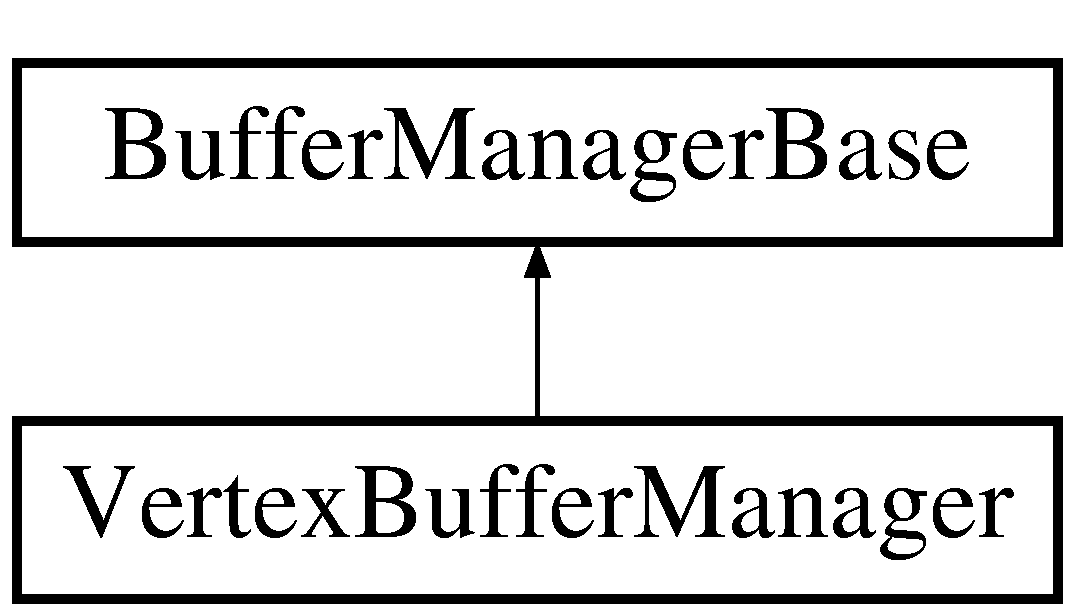
\includegraphics[height=2.000000cm]{d6/dc3/class_vertex_buffer_manager}
\end{center}
\end{figure}
\subsection*{Public Member Functions}
\begin{DoxyCompactItemize}
\item 
\mbox{\hyperlink{stdafx_8h_a8ee2d990c5dfba7794dd2b60741d7722}{D3\+D\+E\+N\+G\+I\+N\+E\+\_\+\+A\+PI}} \mbox{\hyperlink{class_vertex_buffer_manager_afb1c9143a4178c12e95d6d36f98e7f9a}{Vertex\+Buffer\+Manager}} (std\+::shared\+\_\+ptr$<$ std\+::vector$<$ \mbox{\hyperlink{struct_structures_1_1_vertex_tex_coord_normal}{Structures\+::\+Vertex\+Tex\+Coord\+Normal}} $>$$>$ vertices, const std\+::shared\+\_\+ptr$<$ \mbox{\hyperlink{class_d_x_1_1_device_resources}{D\+X\+::\+Device\+Resources}} $>$ device\+Resources, const std\+::shared\+\_\+ptr$<$ \mbox{\hyperlink{class_command_list_manager}{Command\+List\+Manager}} $>$ command\+List\+Manager)
\begin{DoxyCompactList}\small\item\em Construct a new Vertex Buffer Manager\+:\+: Vertex Buffer Manager object. \end{DoxyCompactList}\item 
\mbox{\hyperlink{stdafx_8h_a8ee2d990c5dfba7794dd2b60741d7722}{D3\+D\+E\+N\+G\+I\+N\+E\+\_\+\+A\+PI}} \mbox{\hyperlink{class_vertex_buffer_manager_aa3ff5c3b6cfc0dbe797bb1d953c62616}{$\sim$\+Vertex\+Buffer\+Manager}} ()
\begin{DoxyCompactList}\small\item\em Destroy the Vertex Buffer Manager\+:\+: Vertex Buffer Manager object. \end{DoxyCompactList}\item 
\mbox{\hyperlink{stdafx_8h_a8ee2d990c5dfba7794dd2b60741d7722}{D3\+D\+E\+N\+G\+I\+N\+E\+\_\+\+A\+PI}} D3\+D12\+\_\+\+V\+E\+R\+T\+E\+X\+\_\+\+B\+U\+F\+F\+E\+R\+\_\+\+V\+I\+EW \mbox{\hyperlink{class_vertex_buffer_manager_a164fa0bdbc01ab468792626bd9f9d109}{Create\+Vertex\+Buffer\+View}} () const
\begin{DoxyCompactList}\small\item\em get the vertex buffer view from the vertex buffer \end{DoxyCompactList}\end{DoxyCompactItemize}
\subsection*{Private Attributes}
\begin{DoxyCompactItemize}
\item 
std\+::shared\+\_\+ptr$<$ std\+::vector$<$ \mbox{\hyperlink{struct_structures_1_1_vertex_tex_coord_normal}{Structures\+::\+Vertex\+Tex\+Coord\+Normal}} $>$ $>$ \mbox{\hyperlink{class_vertex_buffer_manager_adbeb6371c5b6dbd5f2adb57273ee342a}{m\+\_\+vertices}}
\item 
size\+\_\+t \mbox{\hyperlink{class_vertex_buffer_manager_a9d499437ec6b54fd97f27a106b0d424a}{m\+\_\+vertices\+Size}}
\begin{DoxyCompactList}\small\item\em vertices \end{DoxyCompactList}\end{DoxyCompactItemize}


\subsection{Detailed Description}


Definition at line 5 of file Vertex\+Buffer\+Manager.\+h.



\subsection{Constructor \& Destructor Documentation}
\mbox{\Hypertarget{class_vertex_buffer_manager_afb1c9143a4178c12e95d6d36f98e7f9a}\label{class_vertex_buffer_manager_afb1c9143a4178c12e95d6d36f98e7f9a}} 
\index{Vertex\+Buffer\+Manager@{Vertex\+Buffer\+Manager}!Vertex\+Buffer\+Manager@{Vertex\+Buffer\+Manager}}
\index{Vertex\+Buffer\+Manager@{Vertex\+Buffer\+Manager}!Vertex\+Buffer\+Manager@{Vertex\+Buffer\+Manager}}
\subsubsection{\texorpdfstring{Vertex\+Buffer\+Manager()}{VertexBufferManager()}}
{\footnotesize\ttfamily Vertex\+Buffer\+Manager\+::\+Vertex\+Buffer\+Manager (\begin{DoxyParamCaption}\item[{std\+::shared\+\_\+ptr$<$ std\+::vector$<$ \mbox{\hyperlink{struct_structures_1_1_vertex_tex_coord_normal}{Structures\+::\+Vertex\+Tex\+Coord\+Normal}} $>$$>$}]{vertices,  }\item[{const std\+::shared\+\_\+ptr$<$ \mbox{\hyperlink{class_d_x_1_1_device_resources}{D\+X\+::\+Device\+Resources}} $>$}]{device\+Resources,  }\item[{const std\+::shared\+\_\+ptr$<$ \mbox{\hyperlink{class_command_list_manager}{Command\+List\+Manager}} $>$}]{command\+List\+Manager }\end{DoxyParamCaption})}



Construct a new Vertex Buffer Manager\+:\+: Vertex Buffer Manager object. 


\begin{DoxyParams}{Parameters}
{\em vertices} & the vertex vector thjat will become the resource \\
\hline
{\em device\+Resources} & \\
\hline
{\em command\+List\+Manager} & \\
\hline
\end{DoxyParams}


Definition at line 12 of file Vertex\+Buffer\+Manager.\+cpp.


\begin{DoxyCode}
13                                                                 :
14     \mbox{\hyperlink{class_buffer_manager_base_a9cec2f80ae72dc972ef6d18ab075ab6c}{BufferManagerBase}}(vertices->size() * \textcolor{keyword}{sizeof} 
      \mbox{\hyperlink{struct_structures_1_1_vertex_tex_coord_normal}{Structures::VertexTexCoordNormal}},
15         \textcolor{keyword}{reinterpret\_cast<}BYTE*\textcolor{keyword}{>}(vertices->data()),
16         D3D12\_RESOURCE\_STATE\_VERTEX\_AND\_CONSTANT\_BUFFER,
17         deviceResources,
18         commandListManager),
19     \mbox{\hyperlink{class_vertex_buffer_manager_adbeb6371c5b6dbd5f2adb57273ee342a}{m\_vertices}}(vertices)
20 \{
21     \mbox{\hyperlink{class_vertex_buffer_manager_a9d499437ec6b54fd97f27a106b0d424a}{m\_verticesSize}} = \mbox{\hyperlink{class_vertex_buffer_manager_adbeb6371c5b6dbd5f2adb57273ee342a}{m\_vertices}}->size();
22 \}
\end{DoxyCode}
\mbox{\Hypertarget{class_vertex_buffer_manager_aa3ff5c3b6cfc0dbe797bb1d953c62616}\label{class_vertex_buffer_manager_aa3ff5c3b6cfc0dbe797bb1d953c62616}} 
\index{Vertex\+Buffer\+Manager@{Vertex\+Buffer\+Manager}!````~Vertex\+Buffer\+Manager@{$\sim$\+Vertex\+Buffer\+Manager}}
\index{````~Vertex\+Buffer\+Manager@{$\sim$\+Vertex\+Buffer\+Manager}!Vertex\+Buffer\+Manager@{Vertex\+Buffer\+Manager}}
\subsubsection{\texorpdfstring{$\sim$\+Vertex\+Buffer\+Manager()}{~VertexBufferManager()}}
{\footnotesize\ttfamily Vertex\+Buffer\+Manager\+::$\sim$\+Vertex\+Buffer\+Manager (\begin{DoxyParamCaption}{ }\end{DoxyParamCaption})}



Destroy the Vertex Buffer Manager\+:\+: Vertex Buffer Manager object. 



Definition at line 27 of file Vertex\+Buffer\+Manager.\+cpp.


\begin{DoxyCode}
28 \{
29     \mbox{\hyperlink{class_vertex_buffer_manager_adbeb6371c5b6dbd5f2adb57273ee342a}{m\_vertices}}->clear();
30 \}
\end{DoxyCode}


\subsection{Member Function Documentation}
\mbox{\Hypertarget{class_vertex_buffer_manager_a164fa0bdbc01ab468792626bd9f9d109}\label{class_vertex_buffer_manager_a164fa0bdbc01ab468792626bd9f9d109}} 
\index{Vertex\+Buffer\+Manager@{Vertex\+Buffer\+Manager}!Create\+Vertex\+Buffer\+View@{Create\+Vertex\+Buffer\+View}}
\index{Create\+Vertex\+Buffer\+View@{Create\+Vertex\+Buffer\+View}!Vertex\+Buffer\+Manager@{Vertex\+Buffer\+Manager}}
\subsubsection{\texorpdfstring{Create\+Vertex\+Buffer\+View()}{CreateVertexBufferView()}}
{\footnotesize\ttfamily D3\+D12\+\_\+\+V\+E\+R\+T\+E\+X\+\_\+\+B\+U\+F\+F\+E\+R\+\_\+\+V\+I\+EW Vertex\+Buffer\+Manager\+::\+Create\+Vertex\+Buffer\+View (\begin{DoxyParamCaption}{ }\end{DoxyParamCaption}) const}



get the vertex buffer view from the vertex buffer 

\begin{DoxyReturn}{Returns}
D3\+D12\+\_\+\+V\+E\+R\+T\+E\+X\+\_\+\+B\+U\+F\+F\+E\+R\+\_\+\+V\+I\+EW the vertex buffer view 
\end{DoxyReturn}


Definition at line 36 of file Vertex\+Buffer\+Manager.\+cpp.


\begin{DoxyCode}
37 \{
38     \textcolor{keyword}{auto} buffer = \mbox{\hyperlink{class_buffer_manager_base_afa03f652ef76e70618f7f112b7da48c5}{GetResource}}();
39     D3D12\_VERTEX\_BUFFER\_VIEW vertexBufferView;
40     vertexBufferView.BufferLocation = buffer->GetGPUVirtualAddress();
41     vertexBufferView.StrideInBytes = \textcolor{keyword}{sizeof}(\mbox{\hyperlink{struct_structures_1_1_vertex_tex_coord_normal}{Structures::VertexTexCoordNormal}}
      );
42     vertexBufferView.SizeInBytes = \textcolor{keyword}{sizeof}(\mbox{\hyperlink{struct_structures_1_1_vertex_tex_coord_normal}{Structures::VertexTexCoordNormal}})
       * \mbox{\hyperlink{class_vertex_buffer_manager_a9d499437ec6b54fd97f27a106b0d424a}{m\_verticesSize}};
43 
44     \textcolor{keywordflow}{return} vertexBufferView;
45 \}
\end{DoxyCode}


\subsection{Member Data Documentation}
\mbox{\Hypertarget{class_vertex_buffer_manager_adbeb6371c5b6dbd5f2adb57273ee342a}\label{class_vertex_buffer_manager_adbeb6371c5b6dbd5f2adb57273ee342a}} 
\index{Vertex\+Buffer\+Manager@{Vertex\+Buffer\+Manager}!m\+\_\+vertices@{m\+\_\+vertices}}
\index{m\+\_\+vertices@{m\+\_\+vertices}!Vertex\+Buffer\+Manager@{Vertex\+Buffer\+Manager}}
\subsubsection{\texorpdfstring{m\+\_\+vertices}{m\_vertices}}
{\footnotesize\ttfamily std\+::shared\+\_\+ptr$<$std\+::vector$<$\mbox{\hyperlink{struct_structures_1_1_vertex_tex_coord_normal}{Structures\+::\+Vertex\+Tex\+Coord\+Normal}}$>$ $>$ Vertex\+Buffer\+Manager\+::m\+\_\+vertices\hspace{0.3cm}{\ttfamily [private]}}



Definition at line 14 of file Vertex\+Buffer\+Manager.\+h.

\mbox{\Hypertarget{class_vertex_buffer_manager_a9d499437ec6b54fd97f27a106b0d424a}\label{class_vertex_buffer_manager_a9d499437ec6b54fd97f27a106b0d424a}} 
\index{Vertex\+Buffer\+Manager@{Vertex\+Buffer\+Manager}!m\+\_\+vertices\+Size@{m\+\_\+vertices\+Size}}
\index{m\+\_\+vertices\+Size@{m\+\_\+vertices\+Size}!Vertex\+Buffer\+Manager@{Vertex\+Buffer\+Manager}}
\subsubsection{\texorpdfstring{m\+\_\+vertices\+Size}{m\_verticesSize}}
{\footnotesize\ttfamily size\+\_\+t Vertex\+Buffer\+Manager\+::m\+\_\+vertices\+Size\hspace{0.3cm}{\ttfamily [private]}}



vertices 



Definition at line 15 of file Vertex\+Buffer\+Manager.\+h.



The documentation for this class was generated from the following files\+:\begin{DoxyCompactItemize}
\item 
D3d\+Engine/\mbox{\hyperlink{_vertex_buffer_manager_8h}{Vertex\+Buffer\+Manager.\+h}}\item 
D3d\+Engine/\mbox{\hyperlink{_vertex_buffer_manager_8cpp}{Vertex\+Buffer\+Manager.\+cpp}}\end{DoxyCompactItemize}

\hypertarget{struct_structures_1_1_vertex_tex_coord_normal}{}\section{Structures\+:\+:Vertex\+Tex\+Coord\+Normal Struct Reference}
\label{struct_structures_1_1_vertex_tex_coord_normal}\index{Structures\+::\+Vertex\+Tex\+Coord\+Normal@{Structures\+::\+Vertex\+Tex\+Coord\+Normal}}


{\ttfamily \#include $<$Structures.\+h$>$}

\subsection*{Public Attributes}
\begin{DoxyCompactItemize}
\item 
Direct\+X\+::\+X\+M\+F\+L\+O\+A\+T3 \mbox{\hyperlink{struct_structures_1_1_vertex_tex_coord_normal_ae9f706af7cd80e03ef433eff59f7419e}{pos}}
\item 
Direct\+X\+::\+X\+M\+F\+L\+O\+A\+T2 \mbox{\hyperlink{struct_structures_1_1_vertex_tex_coord_normal_aed98dc1551d7593c1e84ad7fd56f6779}{tex\+Coord}}
\item 
Direct\+X\+::\+X\+M\+F\+L\+O\+A\+T3 \mbox{\hyperlink{struct_structures_1_1_vertex_tex_coord_normal_a055e66f1a6cbcb24d3377168750e6b19}{normal}}
\item 
X\+M\+F\+L\+O\+A\+T4 \mbox{\hyperlink{struct_structures_1_1_vertex_tex_coord_normal_a3ba02c418d9edfebfd52286419e8f3b7}{weights1}}
\item 
X\+M\+F\+L\+O\+A\+T4 \mbox{\hyperlink{struct_structures_1_1_vertex_tex_coord_normal_a26def3fe41a0899cb7df21c7cdad86ee}{weights2}}
\item 
X\+M\+F\+L\+O\+A\+T4 \mbox{\hyperlink{struct_structures_1_1_vertex_tex_coord_normal_a1911339f710a0a672dbf5287c6cdc59d}{bones1}}
\item 
X\+M\+F\+L\+O\+A\+T4 \mbox{\hyperlink{struct_structures_1_1_vertex_tex_coord_normal_abfdb4cfc7b16955ca6a3ab0b1cf8ac2d}{bones2}}
\item 
int \mbox{\hyperlink{struct_structures_1_1_vertex_tex_coord_normal_af001a3ca7038ebabe7f4b8097a8e44be}{is\+Animated}}
\end{DoxyCompactItemize}


\subsection{Detailed Description}


Definition at line 59 of file Structures.\+h.



\subsection{Member Data Documentation}
\mbox{\Hypertarget{struct_structures_1_1_vertex_tex_coord_normal_a1911339f710a0a672dbf5287c6cdc59d}\label{struct_structures_1_1_vertex_tex_coord_normal_a1911339f710a0a672dbf5287c6cdc59d}} 
\index{Structures\+::\+Vertex\+Tex\+Coord\+Normal@{Structures\+::\+Vertex\+Tex\+Coord\+Normal}!bones1@{bones1}}
\index{bones1@{bones1}!Structures\+::\+Vertex\+Tex\+Coord\+Normal@{Structures\+::\+Vertex\+Tex\+Coord\+Normal}}
\subsubsection{\texorpdfstring{bones1}{bones1}}
{\footnotesize\ttfamily X\+M\+F\+L\+O\+A\+T4 Structures\+::\+Vertex\+Tex\+Coord\+Normal\+::bones1}



Definition at line 66 of file Structures.\+h.

\mbox{\Hypertarget{struct_structures_1_1_vertex_tex_coord_normal_abfdb4cfc7b16955ca6a3ab0b1cf8ac2d}\label{struct_structures_1_1_vertex_tex_coord_normal_abfdb4cfc7b16955ca6a3ab0b1cf8ac2d}} 
\index{Structures\+::\+Vertex\+Tex\+Coord\+Normal@{Structures\+::\+Vertex\+Tex\+Coord\+Normal}!bones2@{bones2}}
\index{bones2@{bones2}!Structures\+::\+Vertex\+Tex\+Coord\+Normal@{Structures\+::\+Vertex\+Tex\+Coord\+Normal}}
\subsubsection{\texorpdfstring{bones2}{bones2}}
{\footnotesize\ttfamily X\+M\+F\+L\+O\+A\+T4 Structures\+::\+Vertex\+Tex\+Coord\+Normal\+::bones2}



Definition at line 67 of file Structures.\+h.

\mbox{\Hypertarget{struct_structures_1_1_vertex_tex_coord_normal_af001a3ca7038ebabe7f4b8097a8e44be}\label{struct_structures_1_1_vertex_tex_coord_normal_af001a3ca7038ebabe7f4b8097a8e44be}} 
\index{Structures\+::\+Vertex\+Tex\+Coord\+Normal@{Structures\+::\+Vertex\+Tex\+Coord\+Normal}!is\+Animated@{is\+Animated}}
\index{is\+Animated@{is\+Animated}!Structures\+::\+Vertex\+Tex\+Coord\+Normal@{Structures\+::\+Vertex\+Tex\+Coord\+Normal}}
\subsubsection{\texorpdfstring{is\+Animated}{isAnimated}}
{\footnotesize\ttfamily int Structures\+::\+Vertex\+Tex\+Coord\+Normal\+::is\+Animated}



Definition at line 68 of file Structures.\+h.

\mbox{\Hypertarget{struct_structures_1_1_vertex_tex_coord_normal_a055e66f1a6cbcb24d3377168750e6b19}\label{struct_structures_1_1_vertex_tex_coord_normal_a055e66f1a6cbcb24d3377168750e6b19}} 
\index{Structures\+::\+Vertex\+Tex\+Coord\+Normal@{Structures\+::\+Vertex\+Tex\+Coord\+Normal}!normal@{normal}}
\index{normal@{normal}!Structures\+::\+Vertex\+Tex\+Coord\+Normal@{Structures\+::\+Vertex\+Tex\+Coord\+Normal}}
\subsubsection{\texorpdfstring{normal}{normal}}
{\footnotesize\ttfamily Direct\+X\+::\+X\+M\+F\+L\+O\+A\+T3 Structures\+::\+Vertex\+Tex\+Coord\+Normal\+::normal}



Definition at line 63 of file Structures.\+h.

\mbox{\Hypertarget{struct_structures_1_1_vertex_tex_coord_normal_ae9f706af7cd80e03ef433eff59f7419e}\label{struct_structures_1_1_vertex_tex_coord_normal_ae9f706af7cd80e03ef433eff59f7419e}} 
\index{Structures\+::\+Vertex\+Tex\+Coord\+Normal@{Structures\+::\+Vertex\+Tex\+Coord\+Normal}!pos@{pos}}
\index{pos@{pos}!Structures\+::\+Vertex\+Tex\+Coord\+Normal@{Structures\+::\+Vertex\+Tex\+Coord\+Normal}}
\subsubsection{\texorpdfstring{pos}{pos}}
{\footnotesize\ttfamily Direct\+X\+::\+X\+M\+F\+L\+O\+A\+T3 Structures\+::\+Vertex\+Tex\+Coord\+Normal\+::pos}



Definition at line 61 of file Structures.\+h.

\mbox{\Hypertarget{struct_structures_1_1_vertex_tex_coord_normal_aed98dc1551d7593c1e84ad7fd56f6779}\label{struct_structures_1_1_vertex_tex_coord_normal_aed98dc1551d7593c1e84ad7fd56f6779}} 
\index{Structures\+::\+Vertex\+Tex\+Coord\+Normal@{Structures\+::\+Vertex\+Tex\+Coord\+Normal}!tex\+Coord@{tex\+Coord}}
\index{tex\+Coord@{tex\+Coord}!Structures\+::\+Vertex\+Tex\+Coord\+Normal@{Structures\+::\+Vertex\+Tex\+Coord\+Normal}}
\subsubsection{\texorpdfstring{tex\+Coord}{texCoord}}
{\footnotesize\ttfamily Direct\+X\+::\+X\+M\+F\+L\+O\+A\+T2 Structures\+::\+Vertex\+Tex\+Coord\+Normal\+::tex\+Coord}



Definition at line 62 of file Structures.\+h.

\mbox{\Hypertarget{struct_structures_1_1_vertex_tex_coord_normal_a3ba02c418d9edfebfd52286419e8f3b7}\label{struct_structures_1_1_vertex_tex_coord_normal_a3ba02c418d9edfebfd52286419e8f3b7}} 
\index{Structures\+::\+Vertex\+Tex\+Coord\+Normal@{Structures\+::\+Vertex\+Tex\+Coord\+Normal}!weights1@{weights1}}
\index{weights1@{weights1}!Structures\+::\+Vertex\+Tex\+Coord\+Normal@{Structures\+::\+Vertex\+Tex\+Coord\+Normal}}
\subsubsection{\texorpdfstring{weights1}{weights1}}
{\footnotesize\ttfamily X\+M\+F\+L\+O\+A\+T4 Structures\+::\+Vertex\+Tex\+Coord\+Normal\+::weights1}



Definition at line 64 of file Structures.\+h.

\mbox{\Hypertarget{struct_structures_1_1_vertex_tex_coord_normal_a26def3fe41a0899cb7df21c7cdad86ee}\label{struct_structures_1_1_vertex_tex_coord_normal_a26def3fe41a0899cb7df21c7cdad86ee}} 
\index{Structures\+::\+Vertex\+Tex\+Coord\+Normal@{Structures\+::\+Vertex\+Tex\+Coord\+Normal}!weights2@{weights2}}
\index{weights2@{weights2}!Structures\+::\+Vertex\+Tex\+Coord\+Normal@{Structures\+::\+Vertex\+Tex\+Coord\+Normal}}
\subsubsection{\texorpdfstring{weights2}{weights2}}
{\footnotesize\ttfamily X\+M\+F\+L\+O\+A\+T4 Structures\+::\+Vertex\+Tex\+Coord\+Normal\+::weights2}



Definition at line 65 of file Structures.\+h.



The documentation for this struct was generated from the following file\+:\begin{DoxyCompactItemize}
\item 
D3d\+Engine/\mbox{\hyperlink{_structures_8h}{Structures.\+h}}\end{DoxyCompactItemize}

\hypertarget{struct_structures_1_1_vertex_tex_coord_normal_bones}{}\section{Structures\+:\+:Vertex\+Tex\+Coord\+Normal\+Bones Struct Reference}
\label{struct_structures_1_1_vertex_tex_coord_normal_bones}\index{Structures\+::\+Vertex\+Tex\+Coord\+Normal\+Bones@{Structures\+::\+Vertex\+Tex\+Coord\+Normal\+Bones}}


{\ttfamily \#include $<$Structures.\+h$>$}

\subsection*{Public Attributes}
\begin{DoxyCompactItemize}
\item 
Direct\+X\+::\+X\+M\+F\+L\+O\+A\+T3 \mbox{\hyperlink{struct_structures_1_1_vertex_tex_coord_normal_bones_a1d797de6d2ae0aa51c08bdec672d30f5}{pos}}
\item 
Direct\+X\+::\+X\+M\+F\+L\+O\+A\+T2 \mbox{\hyperlink{struct_structures_1_1_vertex_tex_coord_normal_bones_abaf5ae6c053da21097793b43e6fe4d7b}{tex\+Coord}}
\item 
Direct\+X\+::\+X\+M\+F\+L\+O\+A\+T3 \mbox{\hyperlink{struct_structures_1_1_vertex_tex_coord_normal_bones_af6cc8525c6e4d5c47bee42857ec81aeb}{normal}}
\item 
std\+::vector$<$ \mbox{\hyperlink{struct_structures_1_1_bone}{Bone}} $>$ \mbox{\hyperlink{struct_structures_1_1_vertex_tex_coord_normal_bones_abcfa247f03b099d663d5206328735845}{bones}}
\end{DoxyCompactItemize}


\subsection{Detailed Description}


Definition at line 52 of file Structures.\+h.



\subsection{Member Data Documentation}
\mbox{\Hypertarget{struct_structures_1_1_vertex_tex_coord_normal_bones_abcfa247f03b099d663d5206328735845}\label{struct_structures_1_1_vertex_tex_coord_normal_bones_abcfa247f03b099d663d5206328735845}} 
\index{Structures\+::\+Vertex\+Tex\+Coord\+Normal\+Bones@{Structures\+::\+Vertex\+Tex\+Coord\+Normal\+Bones}!bones@{bones}}
\index{bones@{bones}!Structures\+::\+Vertex\+Tex\+Coord\+Normal\+Bones@{Structures\+::\+Vertex\+Tex\+Coord\+Normal\+Bones}}
\subsubsection{\texorpdfstring{bones}{bones}}
{\footnotesize\ttfamily std\+::vector$<$\mbox{\hyperlink{struct_structures_1_1_bone}{Bone}}$>$ Structures\+::\+Vertex\+Tex\+Coord\+Normal\+Bones\+::bones}



Definition at line 57 of file Structures.\+h.

\mbox{\Hypertarget{struct_structures_1_1_vertex_tex_coord_normal_bones_af6cc8525c6e4d5c47bee42857ec81aeb}\label{struct_structures_1_1_vertex_tex_coord_normal_bones_af6cc8525c6e4d5c47bee42857ec81aeb}} 
\index{Structures\+::\+Vertex\+Tex\+Coord\+Normal\+Bones@{Structures\+::\+Vertex\+Tex\+Coord\+Normal\+Bones}!normal@{normal}}
\index{normal@{normal}!Structures\+::\+Vertex\+Tex\+Coord\+Normal\+Bones@{Structures\+::\+Vertex\+Tex\+Coord\+Normal\+Bones}}
\subsubsection{\texorpdfstring{normal}{normal}}
{\footnotesize\ttfamily Direct\+X\+::\+X\+M\+F\+L\+O\+A\+T3 Structures\+::\+Vertex\+Tex\+Coord\+Normal\+Bones\+::normal}



Definition at line 56 of file Structures.\+h.

\mbox{\Hypertarget{struct_structures_1_1_vertex_tex_coord_normal_bones_a1d797de6d2ae0aa51c08bdec672d30f5}\label{struct_structures_1_1_vertex_tex_coord_normal_bones_a1d797de6d2ae0aa51c08bdec672d30f5}} 
\index{Structures\+::\+Vertex\+Tex\+Coord\+Normal\+Bones@{Structures\+::\+Vertex\+Tex\+Coord\+Normal\+Bones}!pos@{pos}}
\index{pos@{pos}!Structures\+::\+Vertex\+Tex\+Coord\+Normal\+Bones@{Structures\+::\+Vertex\+Tex\+Coord\+Normal\+Bones}}
\subsubsection{\texorpdfstring{pos}{pos}}
{\footnotesize\ttfamily Direct\+X\+::\+X\+M\+F\+L\+O\+A\+T3 Structures\+::\+Vertex\+Tex\+Coord\+Normal\+Bones\+::pos}



Definition at line 54 of file Structures.\+h.

\mbox{\Hypertarget{struct_structures_1_1_vertex_tex_coord_normal_bones_abaf5ae6c053da21097793b43e6fe4d7b}\label{struct_structures_1_1_vertex_tex_coord_normal_bones_abaf5ae6c053da21097793b43e6fe4d7b}} 
\index{Structures\+::\+Vertex\+Tex\+Coord\+Normal\+Bones@{Structures\+::\+Vertex\+Tex\+Coord\+Normal\+Bones}!tex\+Coord@{tex\+Coord}}
\index{tex\+Coord@{tex\+Coord}!Structures\+::\+Vertex\+Tex\+Coord\+Normal\+Bones@{Structures\+::\+Vertex\+Tex\+Coord\+Normal\+Bones}}
\subsubsection{\texorpdfstring{tex\+Coord}{texCoord}}
{\footnotesize\ttfamily Direct\+X\+::\+X\+M\+F\+L\+O\+A\+T2 Structures\+::\+Vertex\+Tex\+Coord\+Normal\+Bones\+::tex\+Coord}



Definition at line 55 of file Structures.\+h.



The documentation for this struct was generated from the following file\+:\begin{DoxyCompactItemize}
\item 
D3d\+Engine/\mbox{\hyperlink{_structures_8h}{Structures.\+h}}\end{DoxyCompactItemize}

\hypertarget{struct_structures_1_1_vertices_indices}{}\section{Structures\+:\+:Vertices\+Indices Struct Reference}
\label{struct_structures_1_1_vertices_indices}\index{Structures\+::\+Vertices\+Indices@{Structures\+::\+Vertices\+Indices}}


{\ttfamily \#include $<$Structures.\+h$>$}

\subsection*{Public Attributes}
\begin{DoxyCompactItemize}
\item 
std\+::vector$<$ \mbox{\hyperlink{struct_structures_1_1_vertex_tex_coord_normal_bones}{Vertex\+Tex\+Coord\+Normal\+Bones}} $>$ \mbox{\hyperlink{struct_structures_1_1_vertices_indices_a17a49029b0b00cbf9a0670033b338e10}{vertices}}
\item 
std\+::vector$<$ unsigned int $>$ \mbox{\hyperlink{struct_structures_1_1_vertices_indices_a7763f6218cd1e0dda0c0e52444a62b37}{indices}}
\item 
std\+::vector$<$ \mbox{\hyperlink{struct_structures_1_1_animation}{Structures\+::\+Animation}} $>$ \mbox{\hyperlink{struct_structures_1_1_vertices_indices_a3c1b7c206b7b84899cd24fff9e5734f3}{animations}}
\end{DoxyCompactItemize}


\subsection{Detailed Description}


Definition at line 71 of file Structures.\+h.



\subsection{Member Data Documentation}
\mbox{\Hypertarget{struct_structures_1_1_vertices_indices_a3c1b7c206b7b84899cd24fff9e5734f3}\label{struct_structures_1_1_vertices_indices_a3c1b7c206b7b84899cd24fff9e5734f3}} 
\index{Structures\+::\+Vertices\+Indices@{Structures\+::\+Vertices\+Indices}!animations@{animations}}
\index{animations@{animations}!Structures\+::\+Vertices\+Indices@{Structures\+::\+Vertices\+Indices}}
\subsubsection{\texorpdfstring{animations}{animations}}
{\footnotesize\ttfamily std\+::vector$<$\mbox{\hyperlink{struct_structures_1_1_animation}{Structures\+::\+Animation}}$>$ Structures\+::\+Vertices\+Indices\+::animations}



Definition at line 75 of file Structures.\+h.

\mbox{\Hypertarget{struct_structures_1_1_vertices_indices_a7763f6218cd1e0dda0c0e52444a62b37}\label{struct_structures_1_1_vertices_indices_a7763f6218cd1e0dda0c0e52444a62b37}} 
\index{Structures\+::\+Vertices\+Indices@{Structures\+::\+Vertices\+Indices}!indices@{indices}}
\index{indices@{indices}!Structures\+::\+Vertices\+Indices@{Structures\+::\+Vertices\+Indices}}
\subsubsection{\texorpdfstring{indices}{indices}}
{\footnotesize\ttfamily std\+::vector$<$unsigned int$>$ Structures\+::\+Vertices\+Indices\+::indices}



Definition at line 74 of file Structures.\+h.

\mbox{\Hypertarget{struct_structures_1_1_vertices_indices_a17a49029b0b00cbf9a0670033b338e10}\label{struct_structures_1_1_vertices_indices_a17a49029b0b00cbf9a0670033b338e10}} 
\index{Structures\+::\+Vertices\+Indices@{Structures\+::\+Vertices\+Indices}!vertices@{vertices}}
\index{vertices@{vertices}!Structures\+::\+Vertices\+Indices@{Structures\+::\+Vertices\+Indices}}
\subsubsection{\texorpdfstring{vertices}{vertices}}
{\footnotesize\ttfamily std\+::vector$<$\mbox{\hyperlink{struct_structures_1_1_vertex_tex_coord_normal_bones}{Vertex\+Tex\+Coord\+Normal\+Bones}}$>$ Structures\+::\+Vertices\+Indices\+::vertices}



Definition at line 73 of file Structures.\+h.



The documentation for this struct was generated from the following file\+:\begin{DoxyCompactItemize}
\item 
D3d\+Engine/\mbox{\hyperlink{_structures_8h}{Structures.\+h}}\end{DoxyCompactItemize}

\hypertarget{struct_structures_1_1_vertices_indices_from_bin}{}\section{Structures\+:\+:Vertices\+Indices\+From\+Bin Struct Reference}
\label{struct_structures_1_1_vertices_indices_from_bin}\index{Structures\+::\+Vertices\+Indices\+From\+Bin@{Structures\+::\+Vertices\+Indices\+From\+Bin}}


{\ttfamily \#include $<$Structures.\+h$>$}

\subsection*{Public Attributes}
\begin{DoxyCompactItemize}
\item 
std\+::shared\+\_\+ptr$<$ std\+::vector$<$ \mbox{\hyperlink{struct_structures_1_1_vertex_tex_coord_normal}{Vertex\+Tex\+Coord\+Normal}} $>$ $>$ \mbox{\hyperlink{struct_structures_1_1_vertices_indices_from_bin_ae08d7d2a23d9103049738339cfe37728}{vertices}}
\item 
std\+::shared\+\_\+ptr$<$ std\+::vector$<$ unsigned long $>$ $>$ \mbox{\hyperlink{struct_structures_1_1_vertices_indices_from_bin_ad211d683156331f097085628242c82a2}{indices}}
\item 
std\+::shared\+\_\+ptr$<$ std\+::vector$<$ std\+::vector$<$ std\+::vector$<$ X\+M\+M\+A\+T\+R\+IX $>$ $>$ $>$ $>$ \mbox{\hyperlink{struct_structures_1_1_vertices_indices_from_bin_ad28bbb8708747a9cbbdca10e22782dae}{animations}}
\end{DoxyCompactItemize}


\subsection{Detailed Description}


Definition at line 77 of file Structures.\+h.



\subsection{Member Data Documentation}
\mbox{\Hypertarget{struct_structures_1_1_vertices_indices_from_bin_ad28bbb8708747a9cbbdca10e22782dae}\label{struct_structures_1_1_vertices_indices_from_bin_ad28bbb8708747a9cbbdca10e22782dae}} 
\index{Structures\+::\+Vertices\+Indices\+From\+Bin@{Structures\+::\+Vertices\+Indices\+From\+Bin}!animations@{animations}}
\index{animations@{animations}!Structures\+::\+Vertices\+Indices\+From\+Bin@{Structures\+::\+Vertices\+Indices\+From\+Bin}}
\subsubsection{\texorpdfstring{animations}{animations}}
{\footnotesize\ttfamily std\+::shared\+\_\+ptr$<$std\+::vector$<$std\+::vector$<$std\+::vector$<$X\+M\+M\+A\+T\+R\+IX$>$ $>$ $>$ $>$ Structures\+::\+Vertices\+Indices\+From\+Bin\+::animations}



Definition at line 81 of file Structures.\+h.

\mbox{\Hypertarget{struct_structures_1_1_vertices_indices_from_bin_ad211d683156331f097085628242c82a2}\label{struct_structures_1_1_vertices_indices_from_bin_ad211d683156331f097085628242c82a2}} 
\index{Structures\+::\+Vertices\+Indices\+From\+Bin@{Structures\+::\+Vertices\+Indices\+From\+Bin}!indices@{indices}}
\index{indices@{indices}!Structures\+::\+Vertices\+Indices\+From\+Bin@{Structures\+::\+Vertices\+Indices\+From\+Bin}}
\subsubsection{\texorpdfstring{indices}{indices}}
{\footnotesize\ttfamily std\+::shared\+\_\+ptr$<$std\+::vector$<$unsigned long$>$ $>$ Structures\+::\+Vertices\+Indices\+From\+Bin\+::indices}



Definition at line 80 of file Structures.\+h.

\mbox{\Hypertarget{struct_structures_1_1_vertices_indices_from_bin_ae08d7d2a23d9103049738339cfe37728}\label{struct_structures_1_1_vertices_indices_from_bin_ae08d7d2a23d9103049738339cfe37728}} 
\index{Structures\+::\+Vertices\+Indices\+From\+Bin@{Structures\+::\+Vertices\+Indices\+From\+Bin}!vertices@{vertices}}
\index{vertices@{vertices}!Structures\+::\+Vertices\+Indices\+From\+Bin@{Structures\+::\+Vertices\+Indices\+From\+Bin}}
\subsubsection{\texorpdfstring{vertices}{vertices}}
{\footnotesize\ttfamily std\+::shared\+\_\+ptr$<$std\+::vector$<$\mbox{\hyperlink{struct_structures_1_1_vertex_tex_coord_normal}{Vertex\+Tex\+Coord\+Normal}}$>$ $>$ Structures\+::\+Vertices\+Indices\+From\+Bin\+::vertices}



Definition at line 79 of file Structures.\+h.



The documentation for this struct was generated from the following file\+:\begin{DoxyCompactItemize}
\item 
D3d\+Engine/\mbox{\hyperlink{_structures_8h}{Structures.\+h}}\end{DoxyCompactItemize}

\chapter{File Documentation}
\hypertarget{_animation_manager_8cpp}{}\section{D3d\+Engine/\+Animation\+Manager.cpp File Reference}
\label{_animation_manager_8cpp}\index{D3d\+Engine/\+Animation\+Manager.\+cpp@{D3d\+Engine/\+Animation\+Manager.\+cpp}}
{\ttfamily \#include \char`\"{}stdafx.\+h\char`\"{}}\newline
{\ttfamily \#include \char`\"{}Animation\+Manager.\+h\char`\"{}}\newline
{\ttfamily \#include \char`\"{}Model\+Loader.\+h\char`\"{}}\newline

\hypertarget{_animation_manager_8h}{}\section{D3d\+Engine/\+Animation\+Manager.h File Reference}
\label{_animation_manager_8h}\index{D3d\+Engine/\+Animation\+Manager.\+h@{D3d\+Engine/\+Animation\+Manager.\+h}}
{\ttfamily \#include \char`\"{}stdafx.\+h\char`\"{}}\newline
{\ttfamily \#include $<$vector$>$}\newline
{\ttfamily \#include \char`\"{}Structures.\+h\char`\"{}}\newline
\subsection*{Classes}
\begin{DoxyCompactItemize}
\item 
class \mbox{\hyperlink{class_animation_manager}{Animation\+Manager}}
\end{DoxyCompactItemize}

\hypertarget{_binary_model_loader_8cpp}{}\section{D3d\+Engine/\+Binary\+Model\+Loader.cpp File Reference}
\label{_binary_model_loader_8cpp}\index{D3d\+Engine/\+Binary\+Model\+Loader.\+cpp@{D3d\+Engine/\+Binary\+Model\+Loader.\+cpp}}
{\ttfamily \#include \char`\"{}stdafx.\+h\char`\"{}}\newline
{\ttfamily \#include \char`\"{}Binary\+Model\+Loader.\+h\char`\"{}}\newline
{\ttfamily \#include $<$sys/stat.\+h$>$}\newline

\hypertarget{_binary_model_loader_8h}{}\section{D3d\+Engine/\+Binary\+Model\+Loader.h File Reference}
\label{_binary_model_loader_8h}\index{D3d\+Engine/\+Binary\+Model\+Loader.\+h@{D3d\+Engine/\+Binary\+Model\+Loader.\+h}}
{\ttfamily \#include $<$string$>$}\newline
{\ttfamily \#include $<$ios$>$}\newline
{\ttfamily \#include $<$fstream$>$}\newline
{\ttfamily \#include \char`\"{}Structures.\+h\char`\"{}}\newline
\subsection*{Classes}
\begin{DoxyCompactItemize}
\item 
class \mbox{\hyperlink{class_binary_model_loader}{Binary\+Model\+Loader}}
\end{DoxyCompactItemize}

\hypertarget{_buffer_manager_base_8cpp}{}\section{D3d\+Engine/\+Buffer\+Manager\+Base.cpp File Reference}
\label{_buffer_manager_base_8cpp}\index{D3d\+Engine/\+Buffer\+Manager\+Base.\+cpp@{D3d\+Engine/\+Buffer\+Manager\+Base.\+cpp}}
{\ttfamily \#include \char`\"{}stdafx.\+h\char`\"{}}\newline
{\ttfamily \#include \char`\"{}Buffer\+Manager\+Base.\+h\char`\"{}}\newline

\hypertarget{_buffer_manager_base_8h}{}\section{D3d\+Engine/\+Buffer\+Manager\+Base.h File Reference}
\label{_buffer_manager_base_8h}\index{D3d\+Engine/\+Buffer\+Manager\+Base.\+h@{D3d\+Engine/\+Buffer\+Manager\+Base.\+h}}
{\ttfamily \#include \char`\"{}stdafx.\+h\char`\"{}}\newline
{\ttfamily \#include \char`\"{}Device\+Resources.\+h\char`\"{}}\newline
{\ttfamily \#include \char`\"{}Command\+List\+Manager.\+h\char`\"{}}\newline
{\ttfamily \#include \char`\"{}Resource\+Manager.\+h\char`\"{}}\newline
\subsection*{Classes}
\begin{DoxyCompactItemize}
\item 
class \mbox{\hyperlink{class_buffer_manager_base}{Buffer\+Manager\+Base}}
\end{DoxyCompactItemize}

\hypertarget{_camera_helper_8cpp}{}\section{D3d\+Engine/\+Camera\+Helper.cpp File Reference}
\label{_camera_helper_8cpp}\index{D3d\+Engine/\+Camera\+Helper.\+cpp@{D3d\+Engine/\+Camera\+Helper.\+cpp}}
{\ttfamily \#include \char`\"{}stdafx.\+h\char`\"{}}\newline
{\ttfamily \#include \char`\"{}Camera\+Helper.\+h\char`\"{}}\newline


\subsection{Detailed Description}
A helper class which puts the camera at an offset to the player 
\hypertarget{_camera_helper_8h}{}\section{D3d\+Engine/\+Camera\+Helper.h File Reference}
\label{_camera_helper_8h}\index{D3d\+Engine/\+Camera\+Helper.\+h@{D3d\+Engine/\+Camera\+Helper.\+h}}
{\ttfamily \#include \char`\"{}stdafx.\+h\char`\"{}}\newline
{\ttfamily \#include \char`\"{}Structures.\+h\char`\"{}}\newline
{\ttfamily \#include \char`\"{}Model\+View\+Projection\+Manager.\+h\char`\"{}}\newline
{\ttfamily \#include \char`\"{}Terrain\+Collision\+Helper.\+h\char`\"{}}\newline
\subsection*{Classes}
\begin{DoxyCompactItemize}
\item 
class \mbox{\hyperlink{class_camera_helper}{Camera\+Helper}}
\end{DoxyCompactItemize}

\hypertarget{_command_list_manager_8cpp}{}\section{D3d\+Engine/\+Command\+List\+Manager.cpp File Reference}
\label{_command_list_manager_8cpp}\index{D3d\+Engine/\+Command\+List\+Manager.\+cpp@{D3d\+Engine/\+Command\+List\+Manager.\+cpp}}
{\ttfamily \#include \char`\"{}stdafx.\+h\char`\"{}}\newline
{\ttfamily \#include \char`\"{}Command\+List\+Manager.\+h\char`\"{}}\newline
{\ttfamily \#include \char`\"{}Direct\+X\+Helper.\+h\char`\"{}}\newline
{\ttfamily \#include $<$memory$>$}\newline

\hypertarget{_command_list_manager_8h}{}\section{D3d\+Engine/\+Command\+List\+Manager.h File Reference}
\label{_command_list_manager_8h}\index{D3d\+Engine/\+Command\+List\+Manager.\+h@{D3d\+Engine/\+Command\+List\+Manager.\+h}}
{\ttfamily \#include \char`\"{}stdafx.\+h\char`\"{}}\newline
{\ttfamily \#include \char`\"{}Device\+Resources.\+h\char`\"{}}\newline
{\ttfamily \#include $<$memory$>$}\newline
\subsection*{Classes}
\begin{DoxyCompactItemize}
\item 
class \mbox{\hyperlink{class_command_list_manager}{Command\+List\+Manager}}
\end{DoxyCompactItemize}

\hypertarget{_constant_buffer_manager_8h}{}\section{D3d\+Engine/\+Constant\+Buffer\+Manager.h File Reference}
\label{_constant_buffer_manager_8h}\index{D3d\+Engine/\+Constant\+Buffer\+Manager.\+h@{D3d\+Engine/\+Constant\+Buffer\+Manager.\+h}}
{\ttfamily \#include \char`\"{}stdafx.\+h\char`\"{}}\newline
{\ttfamily \#include \char`\"{}Resource\+Manager.\+h\char`\"{}}\newline
{\ttfamily \#include \char`\"{}Direct\+X\+Helper.\+h\char`\"{}}\newline
\subsection*{Classes}
\begin{DoxyCompactItemize}
\item 
class \mbox{\hyperlink{class_constant_buffer_manager}{Constant\+Buffer\+Manager$<$ T\+Data $>$}}
\end{DoxyCompactItemize}

\hypertarget{_d3d_engine_8cpp}{}\section{D3d\+Engine/\+D3d\+Engine.cpp File Reference}
\label{_d3d_engine_8cpp}\index{D3d\+Engine/\+D3d\+Engine.\+cpp@{D3d\+Engine/\+D3d\+Engine.\+cpp}}
{\ttfamily \#include \char`\"{}stdafx.\+h\char`\"{}}\newline

\hypertarget{d3dx12_8h}{}\section{D3d\+Engine/d3dx12.h File Reference}
\label{d3dx12_8h}\index{D3d\+Engine/d3dx12.\+h@{D3d\+Engine/d3dx12.\+h}}
{\ttfamily \#include \char`\"{}d3d12.\+h\char`\"{}}\newline

\hypertarget{_descriptor_heap_manager_8cpp}{}\section{D3d\+Engine/\+Descriptor\+Heap\+Manager.cpp File Reference}
\label{_descriptor_heap_manager_8cpp}\index{D3d\+Engine/\+Descriptor\+Heap\+Manager.\+cpp@{D3d\+Engine/\+Descriptor\+Heap\+Manager.\+cpp}}
{\ttfamily \#include \char`\"{}stdafx.\+h\char`\"{}}\newline
{\ttfamily \#include \char`\"{}Descriptor\+Heap\+Manager.\+h\char`\"{}}\newline
{\ttfamily \#include \char`\"{}Device\+Resources.\+h\char`\"{}}\newline
{\ttfamily \#include \char`\"{}Direct\+X\+Helper.\+h\char`\"{}}\newline
{\ttfamily \#include \char`\"{}Command\+List\+Manager.\+h\char`\"{}}\newline

\hypertarget{_descriptor_heap_manager_8h}{}\section{D3d\+Engine/\+Descriptor\+Heap\+Manager.h File Reference}
\label{_descriptor_heap_manager_8h}\index{D3d\+Engine/\+Descriptor\+Heap\+Manager.\+h@{D3d\+Engine/\+Descriptor\+Heap\+Manager.\+h}}
{\ttfamily \#include \char`\"{}stdafx.\+h\char`\"{}}\newline
{\ttfamily \#include \char`\"{}Device\+Resources.\+h\char`\"{}}\newline
{\ttfamily \#include $<$memory$>$}\newline
{\ttfamily \#include \char`\"{}Command\+List\+Manager.\+h\char`\"{}}\newline
\subsection*{Classes}
\begin{DoxyCompactItemize}
\item 
class \mbox{\hyperlink{class_descriptor_heap_manager}{Descriptor\+Heap\+Manager}}
\end{DoxyCompactItemize}

\hypertarget{_device_resources_8cpp}{}\section{D3d\+Engine/\+Device\+Resources.cpp File Reference}
\label{_device_resources_8cpp}\index{D3d\+Engine/\+Device\+Resources.\+cpp@{D3d\+Engine/\+Device\+Resources.\+cpp}}
{\ttfamily \#include \char`\"{}stdafx.\+h\char`\"{}}\newline
{\ttfamily \#include \char`\"{}Device\+Resources.\+h\char`\"{}}\newline
{\ttfamily \#include \char`\"{}Direct\+X\+Helper.\+h\char`\"{}}\newline

\hypertarget{_device_resources_8h}{}\section{D3d\+Engine/\+Device\+Resources.h File Reference}
\label{_device_resources_8h}\index{D3d\+Engine/\+Device\+Resources.\+h@{D3d\+Engine/\+Device\+Resources.\+h}}
{\ttfamily \#include \char`\"{}stdafx.\+h\char`\"{}}\newline
\subsection*{Classes}
\begin{DoxyCompactItemize}
\item 
class \mbox{\hyperlink{class_d_x_1_1_device_resources}{D\+X\+::\+Device\+Resources}}
\end{DoxyCompactItemize}
\subsection*{Namespaces}
\begin{DoxyCompactItemize}
\item 
 \mbox{\hyperlink{namespace_d_x}{DX}}
\end{DoxyCompactItemize}
\subsection*{Variables}
\begin{DoxyCompactItemize}
\item 
static const U\+I\+NT \mbox{\hyperlink{namespace_d_x_a13eecb6f150dc97fc5c7c8597377d0fb}{D\+X\+::c\+\_\+frame\+Count}} = 3
\end{DoxyCompactItemize}

\hypertarget{_direct_x_helper_8h}{}\section{D3d\+Engine/\+Direct\+X\+Helper.h File Reference}
\label{_direct_x_helper_8h}\index{D3d\+Engine/\+Direct\+X\+Helper.\+h@{D3d\+Engine/\+Direct\+X\+Helper.\+h}}
{\ttfamily \#include \char`\"{}stdafx.\+h\char`\"{}}\newline
\subsection*{Macros}
\begin{DoxyCompactItemize}
\item 
\#define \mbox{\hyperlink{_direct_x_helper_8h_aac0bf77e771c5756a028295b6400839f}{N\+A\+M\+E\+\_\+\+D3\+D12\+\_\+\+O\+B\+J\+E\+CT}}(x)~\mbox{\hyperlink{_direct_x_helper_8h_acafb1288adc883ddbf58b09975dc16b5}{Set\+Name}}(x.\+Get(), L\#x)
\item 
\#define \mbox{\hyperlink{_direct_x_helper_8h_a79a58dc06babec29638083e2d6cab28a}{N\+A\+M\+E\+\_\+\+D3\+D12\+\_\+\+O\+B\+J\+E\+C\+T\+\_\+\+I\+N\+D\+E\+X\+ED}}(x,  n)~\mbox{\hyperlink{_direct_x_helper_8h_a9d72ba78c2685b08518b8d6d978841df}{Set\+Name\+Indexed}}(x\mbox{[}n\mbox{]}.Get(), L\#x, n)
\end{DoxyCompactItemize}
\subsection*{Functions}
\begin{DoxyCompactItemize}
\item 
\mbox{\hyperlink{stdafx_8h_a8ee2d990c5dfba7794dd2b60741d7722}{D3\+D\+E\+N\+G\+I\+N\+E\+\_\+\+A\+PI}} void \mbox{\hyperlink{_direct_x_helper_8h_abca3eeca6b5772a1112e0a9a9e3d9013}{Throw\+If\+Failed}} (H\+R\+E\+S\+U\+LT hr)
\begin{DoxyCompactList}\small\item\em throw exception if failed \end{DoxyCompactList}\item 
\mbox{\hyperlink{stdafx_8h_a8ee2d990c5dfba7794dd2b60741d7722}{D3\+D\+E\+N\+G\+I\+N\+E\+\_\+\+A\+PI}} void \mbox{\hyperlink{_direct_x_helper_8h_ae43aaa2c2b87c4e0260c082d56ab3477}{Get\+Assets\+Path}} (\+\_\+\+Out\+\_\+writes\+\_\+(path\+Size) W\+C\+H\+AR $\ast$path, U\+I\+NT path\+Size)
\begin{DoxyCompactList}\small\item\em get the path that the current E\+XE is in. \end{DoxyCompactList}\item 
\mbox{\hyperlink{stdafx_8h_a8ee2d990c5dfba7794dd2b60741d7722}{D3\+D\+E\+N\+G\+I\+N\+E\+\_\+\+A\+PI}} H\+R\+E\+S\+U\+LT \mbox{\hyperlink{_direct_x_helper_8h_a0ae920cd8d8c647c6e7c9cb2d3b6c4ba}{Read\+Data\+From\+File}} (L\+P\+C\+W\+S\+TR filename, byte $\ast$$\ast$data, U\+I\+NT $\ast$size)
\begin{DoxyCompactList}\small\item\em read the byte data from a file at a give directory \end{DoxyCompactList}\item 
\mbox{\hyperlink{stdafx_8h_a8ee2d990c5dfba7794dd2b60741d7722}{D3\+D\+E\+N\+G\+I\+N\+E\+\_\+\+A\+PI}} void \mbox{\hyperlink{_direct_x_helper_8h_acafb1288adc883ddbf58b09975dc16b5}{Set\+Name}} (I\+D3\+D12\+Object $\ast$, L\+P\+C\+W\+S\+TR)
\begin{DoxyCompactList}\small\item\em assign a debug name to object \end{DoxyCompactList}\item 
\mbox{\hyperlink{stdafx_8h_a8ee2d990c5dfba7794dd2b60741d7722}{D3\+D\+E\+N\+G\+I\+N\+E\+\_\+\+A\+PI}} void \mbox{\hyperlink{_direct_x_helper_8h_a9d72ba78c2685b08518b8d6d978841df}{Set\+Name\+Indexed}} (I\+D3\+D12\+Object $\ast$, L\+P\+C\+W\+S\+TR, U\+I\+NT)
\end{DoxyCompactItemize}


\subsection{Macro Definition Documentation}
\mbox{\Hypertarget{_direct_x_helper_8h_aac0bf77e771c5756a028295b6400839f}\label{_direct_x_helper_8h_aac0bf77e771c5756a028295b6400839f}} 
\index{Direct\+X\+Helper.\+h@{Direct\+X\+Helper.\+h}!N\+A\+M\+E\+\_\+\+D3\+D12\+\_\+\+O\+B\+J\+E\+CT@{N\+A\+M\+E\+\_\+\+D3\+D12\+\_\+\+O\+B\+J\+E\+CT}}
\index{N\+A\+M\+E\+\_\+\+D3\+D12\+\_\+\+O\+B\+J\+E\+CT@{N\+A\+M\+E\+\_\+\+D3\+D12\+\_\+\+O\+B\+J\+E\+CT}!Direct\+X\+Helper.\+h@{Direct\+X\+Helper.\+h}}
\subsubsection{\texorpdfstring{N\+A\+M\+E\+\_\+\+D3\+D12\+\_\+\+O\+B\+J\+E\+CT}{NAME\_D3D12\_OBJECT}}
{\footnotesize\ttfamily \#define N\+A\+M\+E\+\_\+\+D3\+D12\+\_\+\+O\+B\+J\+E\+CT(\begin{DoxyParamCaption}\item[{}]{x }\end{DoxyParamCaption})~\mbox{\hyperlink{_direct_x_helper_8h_acafb1288adc883ddbf58b09975dc16b5}{Set\+Name}}(x.\+Get(), L\#x)}



Definition at line 133 of file Direct\+X\+Helper.\+h.

\mbox{\Hypertarget{_direct_x_helper_8h_a79a58dc06babec29638083e2d6cab28a}\label{_direct_x_helper_8h_a79a58dc06babec29638083e2d6cab28a}} 
\index{Direct\+X\+Helper.\+h@{Direct\+X\+Helper.\+h}!N\+A\+M\+E\+\_\+\+D3\+D12\+\_\+\+O\+B\+J\+E\+C\+T\+\_\+\+I\+N\+D\+E\+X\+ED@{N\+A\+M\+E\+\_\+\+D3\+D12\+\_\+\+O\+B\+J\+E\+C\+T\+\_\+\+I\+N\+D\+E\+X\+ED}}
\index{N\+A\+M\+E\+\_\+\+D3\+D12\+\_\+\+O\+B\+J\+E\+C\+T\+\_\+\+I\+N\+D\+E\+X\+ED@{N\+A\+M\+E\+\_\+\+D3\+D12\+\_\+\+O\+B\+J\+E\+C\+T\+\_\+\+I\+N\+D\+E\+X\+ED}!Direct\+X\+Helper.\+h@{Direct\+X\+Helper.\+h}}
\subsubsection{\texorpdfstring{N\+A\+M\+E\+\_\+\+D3\+D12\+\_\+\+O\+B\+J\+E\+C\+T\+\_\+\+I\+N\+D\+E\+X\+ED}{NAME\_D3D12\_OBJECT\_INDEXED}}
{\footnotesize\ttfamily \#define N\+A\+M\+E\+\_\+\+D3\+D12\+\_\+\+O\+B\+J\+E\+C\+T\+\_\+\+I\+N\+D\+E\+X\+ED(\begin{DoxyParamCaption}\item[{}]{x,  }\item[{}]{n }\end{DoxyParamCaption})~\mbox{\hyperlink{_direct_x_helper_8h_a9d72ba78c2685b08518b8d6d978841df}{Set\+Name\+Indexed}}(x\mbox{[}n\mbox{]}.Get(), L\#x, n)}



Definition at line 134 of file Direct\+X\+Helper.\+h.



\subsection{Function Documentation}
\mbox{\Hypertarget{_direct_x_helper_8h_ae43aaa2c2b87c4e0260c082d56ab3477}\label{_direct_x_helper_8h_ae43aaa2c2b87c4e0260c082d56ab3477}} 
\index{Direct\+X\+Helper.\+h@{Direct\+X\+Helper.\+h}!Get\+Assets\+Path@{Get\+Assets\+Path}}
\index{Get\+Assets\+Path@{Get\+Assets\+Path}!Direct\+X\+Helper.\+h@{Direct\+X\+Helper.\+h}}
\subsubsection{\texorpdfstring{Get\+Assets\+Path()}{GetAssetsPath()}}
{\footnotesize\ttfamily \mbox{\hyperlink{stdafx_8h_a8ee2d990c5dfba7794dd2b60741d7722}{D3\+D\+E\+N\+G\+I\+N\+E\+\_\+\+A\+PI}} void Get\+Assets\+Path (\begin{DoxyParamCaption}\item[{\+\_\+\+Out\+\_\+writes\+\_\+(path\+Size) W\+C\+H\+AR $\ast$}]{path,  }\item[{U\+I\+NT}]{path\+Size }\end{DoxyParamCaption})\hspace{0.3cm}{\ttfamily [inline]}}



get the path that the current E\+XE is in. 


\begin{DoxyParams}{Parameters}
{\em path\+Size} & \\
\hline
\end{DoxyParams}
\begin{DoxyReturn}{Returns}
D3\+D\+E\+N\+G\+I\+N\+E\+\_\+\+A\+PI Get\+Assets\+Path 
\end{DoxyReturn}


Definition at line 36 of file Direct\+X\+Helper.\+h.


\begin{DoxyCode}
37 \{
38     \textcolor{keywordflow}{if} (path == \textcolor{keyword}{nullptr})
39     \{
40         \textcolor{keywordflow}{throw} std::exception();
41     \}
42 
43     DWORD size = GetModuleFileName(\textcolor{keyword}{nullptr}, path, pathSize);
44     \textcolor{keywordflow}{if} (size == 0 || size == pathSize)
45     \{
46         \textcolor{comment}{// Method failed or path was truncated.}
47         \textcolor{keywordflow}{throw} std::exception();
48     \}
49 
50     WCHAR* lastSlash = wcsrchr(path, L\textcolor{charliteral}{'\(\backslash\)\(\backslash\)'});
51     \textcolor{keywordflow}{if} (lastSlash)
52     \{
53         *(lastSlash + 1) = L\textcolor{charliteral}{'\(\backslash\)0'};
54     \}
55 \}
\end{DoxyCode}
\mbox{\Hypertarget{_direct_x_helper_8h_a0ae920cd8d8c647c6e7c9cb2d3b6c4ba}\label{_direct_x_helper_8h_a0ae920cd8d8c647c6e7c9cb2d3b6c4ba}} 
\index{Direct\+X\+Helper.\+h@{Direct\+X\+Helper.\+h}!Read\+Data\+From\+File@{Read\+Data\+From\+File}}
\index{Read\+Data\+From\+File@{Read\+Data\+From\+File}!Direct\+X\+Helper.\+h@{Direct\+X\+Helper.\+h}}
\subsubsection{\texorpdfstring{Read\+Data\+From\+File()}{ReadDataFromFile()}}
{\footnotesize\ttfamily \mbox{\hyperlink{stdafx_8h_a8ee2d990c5dfba7794dd2b60741d7722}{D3\+D\+E\+N\+G\+I\+N\+E\+\_\+\+A\+PI}} H\+R\+E\+S\+U\+LT Read\+Data\+From\+File (\begin{DoxyParamCaption}\item[{L\+P\+C\+W\+S\+TR}]{filename,  }\item[{byte $\ast$$\ast$}]{data,  }\item[{U\+I\+NT $\ast$}]{size }\end{DoxyParamCaption})\hspace{0.3cm}{\ttfamily [inline]}}



read the byte data from a file at a give directory 


\begin{DoxyParams}{Parameters}
{\em filename} & the path and name of the file \\
\hline
{\em data} & the data that will be assigned to at the end (this will constain data after the function has finished kinda) \\
\hline
{\em size} & the size of the file again given value inside this function \\
\hline
\end{DoxyParams}


Definition at line 64 of file Direct\+X\+Helper.\+h.


\begin{DoxyCode}
65 \{
66     \textcolor{keyword}{using namespace }Microsoft::WRL;
67 
68     CREATEFILE2\_EXTENDED\_PARAMETERS extendedParams = \{\};
69     extendedParams.dwSize = \textcolor{keyword}{sizeof}(CREATEFILE2\_EXTENDED\_PARAMETERS);
70     extendedParams.dwFileAttributes = FILE\_ATTRIBUTE\_NORMAL;
71     extendedParams.dwFileFlags = FILE\_FLAG\_SEQUENTIAL\_SCAN;
72     extendedParams.dwSecurityQosFlags = SECURITY\_ANONYMOUS;
73     extendedParams.lpSecurityAttributes = \textcolor{keyword}{nullptr};
74     extendedParams.hTemplateFile = \textcolor{keyword}{nullptr};
75 
76     Wrappers::FileHandle file(CreateFile2(filename, GENERIC\_READ, FILE\_SHARE\_READ, OPEN\_EXISTING, &
      extendedParams));
77     \textcolor{keywordflow}{if} (file.Get() == INVALID\_HANDLE\_VALUE)
78     \{
79         \textcolor{keywordflow}{throw} std::exception();
80     \}
81 
82     FILE\_STANDARD\_INFO fileInfo = \{\};
83     \textcolor{keywordflow}{if} (!GetFileInformationByHandleEx(file.Get(), FileStandardInfo, &fileInfo, \textcolor{keyword}{sizeof}(fileInfo)))
84     \{
85         \textcolor{keywordflow}{throw} std::exception();
86     \}
87 
88     \textcolor{keywordflow}{if} (fileInfo.EndOfFile.HighPart != 0)
89     \{
90         \textcolor{keywordflow}{throw} std::exception();
91     \}
92 
93     *data = \textcolor{keyword}{reinterpret\_cast<}byte*\textcolor{keyword}{>}(malloc(fileInfo.EndOfFile.LowPart));
94     *size = fileInfo.EndOfFile.LowPart;
95 
96     \textcolor{keywordflow}{if} (!ReadFile(file.Get(), *data, fileInfo.EndOfFile.LowPart, \textcolor{keyword}{nullptr}, \textcolor{keyword}{nullptr}))
97     \{
98         \textcolor{keywordflow}{throw} std::exception();
99     \}
100 
101     \textcolor{keywordflow}{return} S\_OK;
102 \}
\end{DoxyCode}
\mbox{\Hypertarget{_direct_x_helper_8h_acafb1288adc883ddbf58b09975dc16b5}\label{_direct_x_helper_8h_acafb1288adc883ddbf58b09975dc16b5}} 
\index{Direct\+X\+Helper.\+h@{Direct\+X\+Helper.\+h}!Set\+Name@{Set\+Name}}
\index{Set\+Name@{Set\+Name}!Direct\+X\+Helper.\+h@{Direct\+X\+Helper.\+h}}
\subsubsection{\texorpdfstring{Set\+Name()}{SetName()}}
{\footnotesize\ttfamily \mbox{\hyperlink{stdafx_8h_a8ee2d990c5dfba7794dd2b60741d7722}{D3\+D\+E\+N\+G\+I\+N\+E\+\_\+\+A\+PI}} void Set\+Name (\begin{DoxyParamCaption}\item[{I\+D3\+D12\+Object $\ast$}]{,  }\item[{L\+P\+C\+W\+S\+TR}]{ }\end{DoxyParamCaption})\hspace{0.3cm}{\ttfamily [inline]}}



assign a debug name to object 



Definition at line 122 of file Direct\+X\+Helper.\+h.


\begin{DoxyCode}
123 \{
124 \}
\end{DoxyCode}
\mbox{\Hypertarget{_direct_x_helper_8h_a9d72ba78c2685b08518b8d6d978841df}\label{_direct_x_helper_8h_a9d72ba78c2685b08518b8d6d978841df}} 
\index{Direct\+X\+Helper.\+h@{Direct\+X\+Helper.\+h}!Set\+Name\+Indexed@{Set\+Name\+Indexed}}
\index{Set\+Name\+Indexed@{Set\+Name\+Indexed}!Direct\+X\+Helper.\+h@{Direct\+X\+Helper.\+h}}
\subsubsection{\texorpdfstring{Set\+Name\+Indexed()}{SetNameIndexed()}}
{\footnotesize\ttfamily \mbox{\hyperlink{stdafx_8h_a8ee2d990c5dfba7794dd2b60741d7722}{D3\+D\+E\+N\+G\+I\+N\+E\+\_\+\+A\+PI}} void Set\+Name\+Indexed (\begin{DoxyParamCaption}\item[{I\+D3\+D12\+Object $\ast$}]{,  }\item[{L\+P\+C\+W\+S\+TR}]{,  }\item[{U\+I\+NT}]{ }\end{DoxyParamCaption})\hspace{0.3cm}{\ttfamily [inline]}}



Definition at line 125 of file Direct\+X\+Helper.\+h.


\begin{DoxyCode}
126 \{
127 \}
\end{DoxyCode}
\mbox{\Hypertarget{_direct_x_helper_8h_abca3eeca6b5772a1112e0a9a9e3d9013}\label{_direct_x_helper_8h_abca3eeca6b5772a1112e0a9a9e3d9013}} 
\index{Direct\+X\+Helper.\+h@{Direct\+X\+Helper.\+h}!Throw\+If\+Failed@{Throw\+If\+Failed}}
\index{Throw\+If\+Failed@{Throw\+If\+Failed}!Direct\+X\+Helper.\+h@{Direct\+X\+Helper.\+h}}
\subsubsection{\texorpdfstring{Throw\+If\+Failed()}{ThrowIfFailed()}}
{\footnotesize\ttfamily \mbox{\hyperlink{stdafx_8h_a8ee2d990c5dfba7794dd2b60741d7722}{D3\+D\+E\+N\+G\+I\+N\+E\+\_\+\+A\+PI}} void Throw\+If\+Failed (\begin{DoxyParamCaption}\item[{H\+R\+E\+S\+U\+LT}]{hr }\end{DoxyParamCaption})\hspace{0.3cm}{\ttfamily [inline]}}



throw exception if failed 


\begin{DoxyParams}{Parameters}
{\em hr} & \\
\hline
\end{DoxyParams}
\begin{DoxyReturn}{Returns}
D3\+D\+E\+N\+G\+I\+N\+E\+\_\+\+A\+PI Throw\+If\+Failed 
\end{DoxyReturn}


Definition at line 20 of file Direct\+X\+Helper.\+h.


\begin{DoxyCode}
21 \{
22     \textcolor{keywordflow}{if} (FAILED(hr))
23     \{
24         \textcolor{keywordflow}{throw} std::exception();
25     \}
26 \}
\end{DoxyCode}

\hypertarget{dllmain_8cpp}{}\section{D3d\+Engine/dllmain.cpp File Reference}
\label{dllmain_8cpp}\index{D3d\+Engine/dllmain.\+cpp@{D3d\+Engine/dllmain.\+cpp}}
{\ttfamily \#include \char`\"{}stdafx.\+h\char`\"{}}\newline
\subsection*{Functions}
\begin{DoxyCompactItemize}
\item 
B\+O\+OL A\+P\+I\+E\+N\+T\+RY \mbox{\hyperlink{dllmain_8cpp_a26e64fb39b69bcd9d1274d279f1561b9}{Dll\+Main}} (H\+M\+O\+D\+U\+LE h\+Module, D\+W\+O\+RD ul\+\_\+reason\+\_\+for\+\_\+call, L\+P\+V\+O\+ID lp\+Reserved)
\end{DoxyCompactItemize}


\subsection{Function Documentation}
\mbox{\Hypertarget{dllmain_8cpp_a26e64fb39b69bcd9d1274d279f1561b9}\label{dllmain_8cpp_a26e64fb39b69bcd9d1274d279f1561b9}} 
\index{dllmain.\+cpp@{dllmain.\+cpp}!Dll\+Main@{Dll\+Main}}
\index{Dll\+Main@{Dll\+Main}!dllmain.\+cpp@{dllmain.\+cpp}}
\subsubsection{\texorpdfstring{Dll\+Main()}{DllMain()}}
{\footnotesize\ttfamily B\+O\+OL A\+P\+I\+E\+N\+T\+RY Dll\+Main (\begin{DoxyParamCaption}\item[{H\+M\+O\+D\+U\+LE}]{h\+Module,  }\item[{D\+W\+O\+RD}]{ul\+\_\+reason\+\_\+for\+\_\+call,  }\item[{L\+P\+V\+O\+ID}]{lp\+Reserved }\end{DoxyParamCaption})}



Definition at line 4 of file dllmain.\+cpp.


\begin{DoxyCode}
8  \{
9 \end{DoxyCode}

\hypertarget{_index_buffer_manager_8cpp}{}\section{D3d\+Engine/\+Index\+Buffer\+Manager.cpp File Reference}
\label{_index_buffer_manager_8cpp}\index{D3d\+Engine/\+Index\+Buffer\+Manager.\+cpp@{D3d\+Engine/\+Index\+Buffer\+Manager.\+cpp}}
{\ttfamily \#include \char`\"{}stdafx.\+h\char`\"{}}\newline
{\ttfamily \#include \char`\"{}Index\+Buffer\+Manager.\+h\char`\"{}}\newline
{\ttfamily \#include \char`\"{}Vertex\+Buffer\+Manager.\+h\char`\"{}}\newline

\hypertarget{_index_buffer_manager_8h}{}\section{D3d\+Engine/\+Index\+Buffer\+Manager.h File Reference}
\label{_index_buffer_manager_8h}\index{D3d\+Engine/\+Index\+Buffer\+Manager.\+h@{D3d\+Engine/\+Index\+Buffer\+Manager.\+h}}
{\ttfamily \#include \char`\"{}Buffer\+Manager\+Base.\+h\char`\"{}}\newline
\subsection*{Classes}
\begin{DoxyCompactItemize}
\item 
class \mbox{\hyperlink{class_index_buffer_manager}{Index\+Buffer\+Manager}}
\end{DoxyCompactItemize}

\hypertarget{_model_loader_8cpp}{}\section{D3d\+Engine/\+Model\+Loader.cpp File Reference}
\label{_model_loader_8cpp}\index{D3d\+Engine/\+Model\+Loader.\+cpp@{D3d\+Engine/\+Model\+Loader.\+cpp}}
{\ttfamily \#include \char`\"{}stdafx.\+h\char`\"{}}\newline
{\ttfamily \#include \char`\"{}Model\+Loader.\+h\char`\"{}}\newline
{\ttfamily \#include \char`\"{}Structures.\+h\char`\"{}}\newline
{\ttfamily \#include $<$assimp/\+Importer.\+hpp$>$}\newline
{\ttfamily \#include $<$assimp/postprocess.\+h$>$}\newline
{\ttfamily \#include $<$assimp/scene.\+h$>$}\newline
{\ttfamily \#include \char`\"{}Direct\+X\+Helper.\+h\char`\"{}}\newline
{\ttfamily \#include \char`\"{}Animation\+Manager.\+h\char`\"{}}\newline
{\ttfamily \#include $<$iostream$>$}\newline

\hypertarget{_model_loader_8h}{}\section{D3d\+Engine/\+Model\+Loader.h File Reference}
\label{_model_loader_8h}\index{D3d\+Engine/\+Model\+Loader.\+h@{D3d\+Engine/\+Model\+Loader.\+h}}
{\ttfamily \#include \char`\"{}Structures.\+h\char`\"{}}\newline
{\ttfamily \#include $<$assimp/scene.\+h$>$}\newline
{\ttfamily \#include \char`\"{}Animation\+Manager.\+h\char`\"{}}\newline
{\ttfamily \#include $<$assimp/matrix4x4.\+h$>$}\newline
\subsection*{Classes}
\begin{DoxyCompactItemize}
\item 
class \mbox{\hyperlink{class_model_loader}{Model\+Loader}}
\begin{DoxyCompactList}\small\item\em deprecated, for use only when coxl loader not working \end{DoxyCompactList}\end{DoxyCompactItemize}

\hypertarget{_model_view_projection_manager_8cpp}{}\section{D3d\+Engine/\+Model\+View\+Projection\+Manager.cpp File Reference}
\label{_model_view_projection_manager_8cpp}\index{D3d\+Engine/\+Model\+View\+Projection\+Manager.\+cpp@{D3d\+Engine/\+Model\+View\+Projection\+Manager.\+cpp}}
{\ttfamily \#include \char`\"{}stdafx.\+h\char`\"{}}\newline
{\ttfamily \#include \char`\"{}Model\+View\+Projection\+Manager.\+h\char`\"{}}\newline

\hypertarget{_model_view_projection_manager_8h}{}\section{D3d\+Engine/\+Model\+View\+Projection\+Manager.h File Reference}
\label{_model_view_projection_manager_8h}\index{D3d\+Engine/\+Model\+View\+Projection\+Manager.\+h@{D3d\+Engine/\+Model\+View\+Projection\+Manager.\+h}}
{\ttfamily \#include \char`\"{}stdafx.\+h\char`\"{}}\newline
{\ttfamily \#include \char`\"{}Structures.\+h\char`\"{}}\newline
\subsection*{Classes}
\begin{DoxyCompactItemize}
\item 
class \mbox{\hyperlink{class_model_view_projection_manager}{Model\+View\+Projection\+Manager}}
\end{DoxyCompactItemize}

\hypertarget{_path_manager_8cpp}{}\section{D3d\+Engine/\+Path\+Manager.cpp File Reference}
\label{_path_manager_8cpp}\index{D3d\+Engine/\+Path\+Manager.\+cpp@{D3d\+Engine/\+Path\+Manager.\+cpp}}
{\ttfamily \#include \char`\"{}stdafx.\+h\char`\"{}}\newline
{\ttfamily \#include \char`\"{}Path\+Manager.\+h\char`\"{}}\newline

\hypertarget{_path_manager_8h}{}\section{D3d\+Engine/\+Path\+Manager.h File Reference}
\label{_path_manager_8h}\index{D3d\+Engine/\+Path\+Manager.\+h@{D3d\+Engine/\+Path\+Manager.\+h}}
{\ttfamily \#include \char`\"{}stdafx.\+h\char`\"{}}\newline
{\ttfamily \#include \char`\"{}Direct\+X\+Helper.\+h\char`\"{}}\newline
\subsection*{Classes}
\begin{DoxyCompactItemize}
\item 
class \mbox{\hyperlink{class_path_manager}{Path\+Manager}}
\end{DoxyCompactItemize}

\hypertarget{_perlin_noise_8cpp}{}\section{D3d\+Engine/\+Perlin\+Noise.cpp File Reference}
\label{_perlin_noise_8cpp}\index{D3d\+Engine/\+Perlin\+Noise.\+cpp@{D3d\+Engine/\+Perlin\+Noise.\+cpp}}
{\ttfamily \#include \char`\"{}stdafx.\+h\char`\"{}}\newline
{\ttfamily \#include \char`\"{}Perlin\+Noise.\+h\char`\"{}}\newline

\hypertarget{_perlin_noise_8h}{}\section{D3d\+Engine/\+Perlin\+Noise.h File Reference}
\label{_perlin_noise_8h}\index{D3d\+Engine/\+Perlin\+Noise.\+h@{D3d\+Engine/\+Perlin\+Noise.\+h}}
\subsection*{Classes}
\begin{DoxyCompactItemize}
\item 
class \mbox{\hyperlink{class_perlin_noise}{Perlin\+Noise}}
\end{DoxyCompactItemize}

\hypertarget{_physics_helper_8cpp}{}\section{D3d\+Engine/\+Physics\+Helper.cpp File Reference}
\label{_physics_helper_8cpp}\index{D3d\+Engine/\+Physics\+Helper.\+cpp@{D3d\+Engine/\+Physics\+Helper.\+cpp}}
{\ttfamily \#include \char`\"{}stdafx.\+h\char`\"{}}\newline
{\ttfamily \#include \char`\"{}Physics\+Helper.\+h\char`\"{}}\newline

\hypertarget{_physics_helper_8h}{}\section{D3d\+Engine/\+Physics\+Helper.h File Reference}
\label{_physics_helper_8h}\index{D3d\+Engine/\+Physics\+Helper.\+h@{D3d\+Engine/\+Physics\+Helper.\+h}}
{\ttfamily \#include \char`\"{}stdafx.\+h\char`\"{}}\newline
\subsection*{Classes}
\begin{DoxyCompactItemize}
\item 
class \mbox{\hyperlink{class_physics_helper}{Physics\+Helper}}
\end{DoxyCompactItemize}

\hypertarget{_p_s_o_manager_8cpp}{}\section{D3d\+Engine/\+P\+S\+O\+Manager.cpp File Reference}
\label{_p_s_o_manager_8cpp}\index{D3d\+Engine/\+P\+S\+O\+Manager.\+cpp@{D3d\+Engine/\+P\+S\+O\+Manager.\+cpp}}
{\ttfamily \#include \char`\"{}stdafx.\+h\char`\"{}}\newline
{\ttfamily \#include \char`\"{}P\+S\+O\+Manager.\+h\char`\"{}}\newline
{\ttfamily \#include \char`\"{}Direct\+X\+Helper.\+h\char`\"{}}\newline
{\ttfamily \#include \char`\"{}Device\+Resources.\+h\char`\"{}}\newline

\hypertarget{_p_s_o_manager_8h}{}\section{D3d\+Engine/\+P\+S\+O\+Manager.h File Reference}
\label{_p_s_o_manager_8h}\index{D3d\+Engine/\+P\+S\+O\+Manager.\+h@{D3d\+Engine/\+P\+S\+O\+Manager.\+h}}
{\ttfamily \#include \char`\"{}stdafx.\+h\char`\"{}}\newline
{\ttfamily \#include \char`\"{}Device\+Resources.\+h\char`\"{}}\newline
\subsection*{Classes}
\begin{DoxyCompactItemize}
\item 
class \mbox{\hyperlink{class_p_s_o_manager}{P\+S\+O\+Manager}}
\end{DoxyCompactItemize}

\hypertarget{_resource_manager_8cpp}{}\section{D3d\+Engine/\+Resource\+Manager.cpp File Reference}
\label{_resource_manager_8cpp}\index{D3d\+Engine/\+Resource\+Manager.\+cpp@{D3d\+Engine/\+Resource\+Manager.\+cpp}}
{\ttfamily \#include \char`\"{}stdafx.\+h\char`\"{}}\newline
{\ttfamily \#include \char`\"{}Resource\+Manager.\+h\char`\"{}}\newline
{\ttfamily \#include \char`\"{}Direct\+X\+Helper.\+h\char`\"{}}\newline

\hypertarget{_resource_manager_8h}{}\section{D3d\+Engine/\+Resource\+Manager.h File Reference}
\label{_resource_manager_8h}\index{D3d\+Engine/\+Resource\+Manager.\+h@{D3d\+Engine/\+Resource\+Manager.\+h}}
{\ttfamily \#include $<$memory$>$}\newline
{\ttfamily \#include \char`\"{}Device\+Resources.\+h\char`\"{}}\newline
{\ttfamily \#include \char`\"{}Command\+List\+Manager.\+h\char`\"{}}\newline
\subsection*{Classes}
\begin{DoxyCompactItemize}
\item 
class \mbox{\hyperlink{class_resource_manager}{Resource\+Manager}}
\end{DoxyCompactItemize}

\hypertarget{_root_signature_manager_8cpp}{}\section{D3d\+Engine/\+Root\+Signature\+Manager.cpp File Reference}
\label{_root_signature_manager_8cpp}\index{D3d\+Engine/\+Root\+Signature\+Manager.\+cpp@{D3d\+Engine/\+Root\+Signature\+Manager.\+cpp}}
{\ttfamily \#include \char`\"{}stdafx.\+h\char`\"{}}\newline
{\ttfamily \#include \char`\"{}Root\+Signature\+Manager.\+h\char`\"{}}\newline
{\ttfamily \#include \char`\"{}Direct\+X\+Helper.\+h\char`\"{}}\newline
{\ttfamily \#include \char`\"{}Device\+Resources.\+h\char`\"{}}\newline

\hypertarget{_root_signature_manager_8h}{}\section{D3d\+Engine/\+Root\+Signature\+Manager.h File Reference}
\label{_root_signature_manager_8h}\index{D3d\+Engine/\+Root\+Signature\+Manager.\+h@{D3d\+Engine/\+Root\+Signature\+Manager.\+h}}
{\ttfamily \#include \char`\"{}stdafx.\+h\char`\"{}}\newline
{\ttfamily \#include \char`\"{}Device\+Resources.\+h\char`\"{}}\newline
{\ttfamily \#include $<$memory$>$}\newline
{\ttfamily \#include $<$vector$>$}\newline
\subsection*{Classes}
\begin{DoxyCompactItemize}
\item 
class \mbox{\hyperlink{class_root_parameter}{Root\+Parameter}}
\item 
class \mbox{\hyperlink{class_root_signature}{Root\+Signature}}
\item 
class \mbox{\hyperlink{class_root_signature_manager}{Root\+Signature\+Manager}}
\end{DoxyCompactItemize}

\hypertarget{_shader_loader_8cpp}{}\section{D3d\+Engine/\+Shader\+Loader.cpp File Reference}
\label{_shader_loader_8cpp}\index{D3d\+Engine/\+Shader\+Loader.\+cpp@{D3d\+Engine/\+Shader\+Loader.\+cpp}}
{\ttfamily \#include \char`\"{}stdafx.\+h\char`\"{}}\newline
{\ttfamily \#include \char`\"{}Shader\+Loader.\+h\char`\"{}}\newline
{\ttfamily \#include $<$string$>$}\newline
{\ttfamily \#include \char`\"{}Direct\+X\+Helper.\+h\char`\"{}}\newline

\hypertarget{_shader_loader_8h}{}\section{D3d\+Engine/\+Shader\+Loader.h File Reference}
\label{_shader_loader_8h}\index{D3d\+Engine/\+Shader\+Loader.\+h@{D3d\+Engine/\+Shader\+Loader.\+h}}
{\ttfamily \#include \char`\"{}Model\+Loader.\+h\char`\"{}}\newline
\subsection*{Classes}
\begin{DoxyCompactItemize}
\item 
class \mbox{\hyperlink{class_shader_loader}{Shader\+Loader}}
\end{DoxyCompactItemize}

\hypertarget{stdafx_8cpp}{}\section{D3d\+Engine/stdafx.cpp File Reference}
\label{stdafx_8cpp}\index{D3d\+Engine/stdafx.\+cpp@{D3d\+Engine/stdafx.\+cpp}}
{\ttfamily \#include \char`\"{}stdafx.\+h\char`\"{}}\newline

\hypertarget{stdafx_8h}{}\section{D3d\+Engine/stdafx.h File Reference}
\label{stdafx_8h}\index{D3d\+Engine/stdafx.\+h@{D3d\+Engine/stdafx.\+h}}
{\ttfamily \#include $<$windowsx.\+h$>$}\newline
{\ttfamily \#include $<$windows.\+h$>$}\newline
{\ttfamily \#include $<$memory$>$}\newline
{\ttfamily \#include $<$d3d12.\+h$>$}\newline
{\ttfamily \#include $<$wincodec.\+h$>$}\newline
{\ttfamily \#include $<$dxgi1\+\_\+4.\+h$>$}\newline
{\ttfamily \#include $<$dxgi.\+h$>$}\newline
{\ttfamily \#include $<$D3\+Dcompiler.\+h$>$}\newline
{\ttfamily \#include $<$Direct\+X\+Math.\+h$>$}\newline
{\ttfamily \#include $<$Direct\+X\+Colors.\+h$>$}\newline
{\ttfamily \#include $<$Direct\+X\+Collision.\+h$>$}\newline
{\ttfamily \#include \char`\"{}d3dx12.\+h\char`\"{}}\newline
{\ttfamily \#include $<$vector$>$}\newline
{\ttfamily \#include $<$string$>$}\newline
{\ttfamily \#include $<$wrl.\+h$>$}\newline
{\ttfamily \#include $<$shellapi.\+h$>$}\newline
\subsection*{Macros}
\begin{DoxyCompactItemize}
\item 
\#define \mbox{\hyperlink{stdafx_8h_a8ee2d990c5dfba7794dd2b60741d7722}{D3\+D\+E\+N\+G\+I\+N\+E\+\_\+\+A\+PI}}~\+\_\+\+\_\+declspec(dllimport)
\item 
\#define \mbox{\hyperlink{stdafx_8h_ac7bef5d85e3dcd73eef56ad39ffc84a9}{W\+I\+N32\+\_\+\+L\+E\+A\+N\+\_\+\+A\+N\+D\+\_\+\+M\+E\+AN}}
\end{DoxyCompactItemize}


\subsection{Macro Definition Documentation}
\mbox{\Hypertarget{stdafx_8h_a8ee2d990c5dfba7794dd2b60741d7722}\label{stdafx_8h_a8ee2d990c5dfba7794dd2b60741d7722}} 
\index{stdafx.\+h@{stdafx.\+h}!D3\+D\+E\+N\+G\+I\+N\+E\+\_\+\+A\+PI@{D3\+D\+E\+N\+G\+I\+N\+E\+\_\+\+A\+PI}}
\index{D3\+D\+E\+N\+G\+I\+N\+E\+\_\+\+A\+PI@{D3\+D\+E\+N\+G\+I\+N\+E\+\_\+\+A\+PI}!stdafx.\+h@{stdafx.\+h}}
\subsubsection{\texorpdfstring{D3\+D\+E\+N\+G\+I\+N\+E\+\_\+\+A\+PI}{D3DENGINE\_API}}
{\footnotesize\ttfamily \#define D3\+D\+E\+N\+G\+I\+N\+E\+\_\+\+A\+PI~\+\_\+\+\_\+declspec(dllimport)}



Definition at line 5 of file stdafx.\+h.

\mbox{\Hypertarget{stdafx_8h_ac7bef5d85e3dcd73eef56ad39ffc84a9}\label{stdafx_8h_ac7bef5d85e3dcd73eef56ad39ffc84a9}} 
\index{stdafx.\+h@{stdafx.\+h}!W\+I\+N32\+\_\+\+L\+E\+A\+N\+\_\+\+A\+N\+D\+\_\+\+M\+E\+AN@{W\+I\+N32\+\_\+\+L\+E\+A\+N\+\_\+\+A\+N\+D\+\_\+\+M\+E\+AN}}
\index{W\+I\+N32\+\_\+\+L\+E\+A\+N\+\_\+\+A\+N\+D\+\_\+\+M\+E\+AN@{W\+I\+N32\+\_\+\+L\+E\+A\+N\+\_\+\+A\+N\+D\+\_\+\+M\+E\+AN}!stdafx.\+h@{stdafx.\+h}}
\subsubsection{\texorpdfstring{W\+I\+N32\+\_\+\+L\+E\+A\+N\+\_\+\+A\+N\+D\+\_\+\+M\+E\+AN}{WIN32\_LEAN\_AND\_MEAN}}
{\footnotesize\ttfamily \#define W\+I\+N32\+\_\+\+L\+E\+A\+N\+\_\+\+A\+N\+D\+\_\+\+M\+E\+AN}



Definition at line 8 of file stdafx.\+h.


\hypertarget{_structures_8h}{}\section{D3d\+Engine/\+Structures.h File Reference}
\label{_structures_8h}\index{D3d\+Engine/\+Structures.\+h@{D3d\+Engine/\+Structures.\+h}}
{\ttfamily \#include \char`\"{}stdafx.\+h\char`\"{}}\newline
{\ttfamily \#include $<$vector$>$}\newline
{\ttfamily \#include \char`\"{}Root\+Signature\+Manager.\+h\char`\"{}}\newline
{\ttfamily \#include $<$map$>$}\newline
{\ttfamily \#include $<$assimp/mesh.\+h$>$}\newline
\subsection*{Classes}
\begin{DoxyCompactItemize}
\item 
struct \mbox{\hyperlink{struct_structures_1_1_anim_frame_bone}{Structures\+::\+Anim\+Frame\+Bone}}
\item 
struct \mbox{\hyperlink{struct_structures_1_1_anim_transforms}{Structures\+::\+Anim\+Transforms}}
\item 
struct \mbox{\hyperlink{struct_structures_1_1_anim_bone}{Structures\+::\+Anim\+Bone}}
\item 
struct \mbox{\hyperlink{struct_structures_1_1assimp_vertex_weight}{Structures\+::assimp\+Vertex\+Weight}}
\item 
struct \mbox{\hyperlink{struct_structures_1_1assimp_bone}{Structures\+::assimp\+Bone}}
\item 
struct \mbox{\hyperlink{struct_structures_1_1_animation}{Structures\+::\+Animation}}
\item 
struct \mbox{\hyperlink{struct_structures_1_1_bone}{Structures\+::\+Bone}}
\item 
struct \mbox{\hyperlink{struct_structures_1_1_vertex_tex_coord_normal_bones}{Structures\+::\+Vertex\+Tex\+Coord\+Normal\+Bones}}
\item 
struct \mbox{\hyperlink{struct_structures_1_1_vertex_tex_coord_normal}{Structures\+::\+Vertex\+Tex\+Coord\+Normal}}
\item 
struct \mbox{\hyperlink{struct_structures_1_1_vertices_indices}{Structures\+::\+Vertices\+Indices}}
\item 
struct \mbox{\hyperlink{struct_structures_1_1_vertices_indices_from_bin}{Structures\+::\+Vertices\+Indices\+From\+Bin}}
\item 
struct \mbox{\hyperlink{struct_structures_1_1_shader_data}{Structures\+::\+Shader\+Data}}
\item 
struct \mbox{\hyperlink{struct_structures_1_1_model_view_projection_constant_buffer}{Structures\+::\+Model\+View\+Projection\+Constant\+Buffer}}
\item 
struct \mbox{\hyperlink{struct_structures_1_1_height_map_info}{Structures\+::\+Height\+Map\+Info}}
\end{DoxyCompactItemize}
\subsection*{Namespaces}
\begin{DoxyCompactItemize}
\item 
 \mbox{\hyperlink{namespace_structures}{Structures}}
\end{DoxyCompactItemize}

\hypertarget{targetver_8h}{}\section{D3d\+Engine/targetver.h File Reference}
\label{targetver_8h}\index{D3d\+Engine/targetver.\+h@{D3d\+Engine/targetver.\+h}}
{\ttfamily \#include $<$S\+D\+K\+D\+D\+K\+Ver.\+h$>$}\newline

\hypertarget{_terrain_collision_helper_8cpp}{}\section{D3d\+Engine/\+Terrain\+Collision\+Helper.cpp File Reference}
\label{_terrain_collision_helper_8cpp}\index{D3d\+Engine/\+Terrain\+Collision\+Helper.\+cpp@{D3d\+Engine/\+Terrain\+Collision\+Helper.\+cpp}}
{\ttfamily \#include \char`\"{}stdafx.\+h\char`\"{}}\newline
{\ttfamily \#include \char`\"{}Terrain\+Collision\+Helper.\+h\char`\"{}}\newline
{\ttfamily \#include \char`\"{}Structures.\+h\char`\"{}}\newline
{\ttfamily \#include \char`\"{}Terrain\+Generation\+Helper.\+h\char`\"{}}\newline

\hypertarget{_terrain_collision_helper_8h}{}\section{D3d\+Engine/\+Terrain\+Collision\+Helper.h File Reference}
\label{_terrain_collision_helper_8h}\index{D3d\+Engine/\+Terrain\+Collision\+Helper.\+h@{D3d\+Engine/\+Terrain\+Collision\+Helper.\+h}}
{\ttfamily \#include \char`\"{}stdafx.\+h\char`\"{}}\newline
\subsection*{Classes}
\begin{DoxyCompactItemize}
\item 
class \mbox{\hyperlink{class_terrain_collision_helper}{Terrain\+Collision\+Helper}}
\end{DoxyCompactItemize}

\hypertarget{_terrain_generation_helper_8cpp}{}\section{D3d\+Engine/\+Terrain\+Generation\+Helper.cpp File Reference}
\label{_terrain_generation_helper_8cpp}\index{D3d\+Engine/\+Terrain\+Generation\+Helper.\+cpp@{D3d\+Engine/\+Terrain\+Generation\+Helper.\+cpp}}
{\ttfamily \#include \char`\"{}stdafx.\+h\char`\"{}}\newline
{\ttfamily \#include \char`\"{}Terrain\+Generation\+Helper.\+h\char`\"{}}\newline

\hypertarget{_terrain_generation_helper_8h}{}\section{D3d\+Engine/\+Terrain\+Generation\+Helper.h File Reference}
\label{_terrain_generation_helper_8h}\index{D3d\+Engine/\+Terrain\+Generation\+Helper.\+h@{D3d\+Engine/\+Terrain\+Generation\+Helper.\+h}}
{\ttfamily \#include \char`\"{}stdafx.\+h\char`\"{}}\newline
{\ttfamily \#include \char`\"{}Perlin\+Noise.\+h\char`\"{}}\newline
{\ttfamily \#include \char`\"{}Structures.\+h\char`\"{}}\newline
\subsection*{Classes}
\begin{DoxyCompactItemize}
\item 
class \mbox{\hyperlink{class_terrain_generation_helper}{Terrain\+Generation\+Helper}}
\end{DoxyCompactItemize}
\subsection*{Macros}
\begin{DoxyCompactItemize}
\item 
\#define \mbox{\hyperlink{_terrain_generation_helper_8h_ad04a251ab3e1323474688977de1579e4}{T\+E\+R\+R\+A\+I\+N\+\_\+\+S\+T\+E\+P\+\_\+\+S\+I\+ZE}}~5
\end{DoxyCompactItemize}


\subsection{Macro Definition Documentation}
\mbox{\Hypertarget{_terrain_generation_helper_8h_ad04a251ab3e1323474688977de1579e4}\label{_terrain_generation_helper_8h_ad04a251ab3e1323474688977de1579e4}} 
\index{Terrain\+Generation\+Helper.\+h@{Terrain\+Generation\+Helper.\+h}!T\+E\+R\+R\+A\+I\+N\+\_\+\+S\+T\+E\+P\+\_\+\+S\+I\+ZE@{T\+E\+R\+R\+A\+I\+N\+\_\+\+S\+T\+E\+P\+\_\+\+S\+I\+ZE}}
\index{T\+E\+R\+R\+A\+I\+N\+\_\+\+S\+T\+E\+P\+\_\+\+S\+I\+ZE@{T\+E\+R\+R\+A\+I\+N\+\_\+\+S\+T\+E\+P\+\_\+\+S\+I\+ZE}!Terrain\+Generation\+Helper.\+h@{Terrain\+Generation\+Helper.\+h}}
\subsubsection{\texorpdfstring{T\+E\+R\+R\+A\+I\+N\+\_\+\+S\+T\+E\+P\+\_\+\+S\+I\+ZE}{TERRAIN\_STEP\_SIZE}}
{\footnotesize\ttfamily \#define T\+E\+R\+R\+A\+I\+N\+\_\+\+S\+T\+E\+P\+\_\+\+S\+I\+ZE~5}



Definition at line 5 of file Terrain\+Generation\+Helper.\+h.


\hypertarget{_texture_loader_8cpp}{}\section{D3d\+Engine/\+Texture\+Loader.cpp File Reference}
\label{_texture_loader_8cpp}\index{D3d\+Engine/\+Texture\+Loader.\+cpp@{D3d\+Engine/\+Texture\+Loader.\+cpp}}
{\ttfamily \#include \char`\"{}stdafx.\+h\char`\"{}}\newline
{\ttfamily \#include \char`\"{}Texture\+Loader.\+h\char`\"{}}\newline

\hypertarget{_texture_loader_8h}{}\section{D3d\+Engine/\+Texture\+Loader.h File Reference}
\label{_texture_loader_8h}\index{D3d\+Engine/\+Texture\+Loader.\+h@{D3d\+Engine/\+Texture\+Loader.\+h}}
\subsection*{Classes}
\begin{DoxyCompactItemize}
\item 
class \mbox{\hyperlink{class_texture_loader}{Texture\+Loader}}
\end{DoxyCompactItemize}

\hypertarget{_texture_resource_manager_8cpp}{}\section{D3d\+Engine/\+Texture\+Resource\+Manager.cpp File Reference}
\label{_texture_resource_manager_8cpp}\index{D3d\+Engine/\+Texture\+Resource\+Manager.\+cpp@{D3d\+Engine/\+Texture\+Resource\+Manager.\+cpp}}
{\ttfamily \#include \char`\"{}stdafx.\+h\char`\"{}}\newline
{\ttfamily \#include \char`\"{}Texture\+Resource\+Manager.\+h\char`\"{}}\newline
{\ttfamily \#include \char`\"{}Texture\+Loader.\+h\char`\"{}}\newline

\hypertarget{_texture_resource_manager_8h}{}\section{D3d\+Engine/\+Texture\+Resource\+Manager.h File Reference}
\label{_texture_resource_manager_8h}\index{D3d\+Engine/\+Texture\+Resource\+Manager.\+h@{D3d\+Engine/\+Texture\+Resource\+Manager.\+h}}
{\ttfamily \#include \char`\"{}stdafx.\+h\char`\"{}}\newline
{\ttfamily \#include \char`\"{}Device\+Resources.\+h\char`\"{}}\newline
{\ttfamily \#include \char`\"{}Command\+List\+Manager.\+h\char`\"{}}\newline
{\ttfamily \#include \char`\"{}Resource\+Manager.\+h\char`\"{}}\newline
\subsection*{Classes}
\begin{DoxyCompactItemize}
\item 
class \mbox{\hyperlink{class_texture_resource_manager}{Texture\+Resource\+Manager}}
\item 
struct \mbox{\hyperlink{struct_texture_resource_manager_1_1_loaded_data}{Texture\+Resource\+Manager\+::\+Loaded\+Data}}
\end{DoxyCompactItemize}

\hypertarget{_vertex_buffer_manager_8cpp}{}\section{D3d\+Engine/\+Vertex\+Buffer\+Manager.cpp File Reference}
\label{_vertex_buffer_manager_8cpp}\index{D3d\+Engine/\+Vertex\+Buffer\+Manager.\+cpp@{D3d\+Engine/\+Vertex\+Buffer\+Manager.\+cpp}}
{\ttfamily \#include \char`\"{}stdafx.\+h\char`\"{}}\newline
{\ttfamily \#include \char`\"{}Vertex\+Buffer\+Manager.\+h\char`\"{}}\newline
{\ttfamily \#include \char`\"{}Structures.\+h\char`\"{}}\newline

\hypertarget{_vertex_buffer_manager_8h}{}\section{D3d\+Engine/\+Vertex\+Buffer\+Manager.h File Reference}
\label{_vertex_buffer_manager_8h}\index{D3d\+Engine/\+Vertex\+Buffer\+Manager.\+h@{D3d\+Engine/\+Vertex\+Buffer\+Manager.\+h}}
{\ttfamily \#include \char`\"{}Buffer\+Manager\+Base.\+h\char`\"{}}\newline
{\ttfamily \#include \char`\"{}Structures.\+h\char`\"{}}\newline
\subsection*{Classes}
\begin{DoxyCompactItemize}
\item 
class \mbox{\hyperlink{class_vertex_buffer_manager}{Vertex\+Buffer\+Manager}}
\end{DoxyCompactItemize}

%--- End generated contents ---

% Index
\backmatter
\newpage
\phantomsection
\clearemptydoublepage
\addcontentsline{toc}{chapter}{Index}
\printindex

\end{document}
